\documentclass[]{book}
\usepackage{lmodern}
\usepackage{amssymb,amsmath}
\usepackage{ifxetex,ifluatex}
\usepackage{fixltx2e} % provides \textsubscript
\ifnum 0\ifxetex 1\fi\ifluatex 1\fi=0 % if pdftex
  \usepackage[T1]{fontenc}
  \usepackage[utf8]{inputenc}
\else % if luatex or xelatex
  \ifxetex
    \usepackage{mathspec}
  \else
    \usepackage{fontspec}
  \fi
  \defaultfontfeatures{Ligatures=TeX,Scale=MatchLowercase}
\fi
% use upquote if available, for straight quotes in verbatim environments
\IfFileExists{upquote.sty}{\usepackage{upquote}}{}
% use microtype if available
\IfFileExists{microtype.sty}{%
\usepackage{microtype}
\UseMicrotypeSet[protrusion]{basicmath} % disable protrusion for tt fonts
}{}
\usepackage[margin=1in]{geometry}
\usepackage{hyperref}
\hypersetup{unicode=true,
            pdftitle={GAMA 1.8 - GAML User Manual for Beginners},
            pdfauthor={Srirama Bhamidipati},
            pdfborder={0 0 0},
            breaklinks=true}
\urlstyle{same}  % don't use monospace font for urls
\usepackage{natbib}
\bibliographystyle{plainnat}
\usepackage{longtable,booktabs}
\usepackage{graphicx,grffile}
\makeatletter
\def\maxwidth{\ifdim\Gin@nat@width>\linewidth\linewidth\else\Gin@nat@width\fi}
\def\maxheight{\ifdim\Gin@nat@height>\textheight\textheight\else\Gin@nat@height\fi}
\makeatother
% Scale images if necessary, so that they will not overflow the page
% margins by default, and it is still possible to overwrite the defaults
% using explicit options in \includegraphics[width, height, ...]{}
\setkeys{Gin}{width=\maxwidth,height=\maxheight,keepaspectratio}
\IfFileExists{parskip.sty}{%
\usepackage{parskip}
}{% else
\setlength{\parindent}{0pt}
\setlength{\parskip}{6pt plus 2pt minus 1pt}
}
\setlength{\emergencystretch}{3em}  % prevent overfull lines
\providecommand{\tightlist}{%
  \setlength{\itemsep}{0pt}\setlength{\parskip}{0pt}}
\setcounter{secnumdepth}{5}
% Redefines (sub)paragraphs to behave more like sections
\ifx\paragraph\undefined\else
\let\oldparagraph\paragraph
\renewcommand{\paragraph}[1]{\oldparagraph{#1}\mbox{}}
\fi
\ifx\subparagraph\undefined\else
\let\oldsubparagraph\subparagraph
\renewcommand{\subparagraph}[1]{\oldsubparagraph{#1}\mbox{}}
\fi

%%% Use protect on footnotes to avoid problems with footnotes in titles
\let\rmarkdownfootnote\footnote%
\def\footnote{\protect\rmarkdownfootnote}

%%% Change title format to be more compact
\usepackage{titling}

% Create subtitle command for use in maketitle
\newcommand{\subtitle}[1]{
  \posttitle{
    \begin{center}\large#1\end{center}
    }
}

\setlength{\droptitle}{-2em}

  \title{GAMA 1.8 - GAML User Manual for Beginners}
    \pretitle{\vspace{\droptitle}\centering\huge}
  \posttitle{\par}
    \author{Srirama Bhamidipati}
    \preauthor{\centering\large\emph}
  \postauthor{\par}
      \predate{\centering\large\emph}
  \postdate{\par}
    \date{Updated: 2018-12-30 (Amsterdam)}

\usepackage{makeidx}
\makeindex

\usepackage{amsthm}
\newtheorem{theorem}{Theorem}[chapter]
\newtheorem{lemma}{Lemma}[chapter]
\theoremstyle{definition}
\newtheorem{definition}{Definition}[chapter]
\newtheorem{corollary}{Corollary}[chapter]
\newtheorem{proposition}{Proposition}[chapter]
\theoremstyle{definition}
\newtheorem{example}{Example}[chapter]
\theoremstyle{definition}
\newtheorem{exercise}{Exercise}[chapter]
\theoremstyle{remark}
\newtheorem*{remark}{Remark}
\newtheorem*{solution}{Solution}
\begin{document}
\maketitle

{
\setcounter{tocdepth}{1}
\tableofcontents
}
\hypertarget{notice}{%
\chapter*{Notice}\label{notice}}
\addcontentsline{toc}{chapter}{Notice}

\begin{itemize}
\item
  The main purpose of this book is to provide a simple introduction with
  bare minimum content that helps the reader to get started with GAMA
  Language (GAML).
\item
  The content of this manual is from gama-platform.org website. I have
  modified and edited portions of the content to give a cleaner format.
\item
  This is a modified content and is not a 100\% reproduction. If you do
  not find what you are looking for, go to the main website.
\item
  I thank the Team of GAMA-Platform for giving me the permission to
  reproduce their content.
\end{itemize}

Cheers !\\
~\\
\textbf{Srirama Bhamidipati}\\
\emph{Delft, Netherlands}\\
\emph{2018}


\includegraphics{gamacover.png}

\hypertarget{report-errors-give-feedback}{%
\chapter*{Report Errors/ Give
Feedback}\label{report-errors-give-feedback}}
\addcontentsline{toc}{chapter}{Report Errors/ Give Feedback}

If you find any problems/typos/errors related to this book, you can
report issues on this
\href{https://github.com/sriramab/gama_books/issues}{page}. On this page
you can click the big green button ``New Issue'' and fill in the
details. Typically, you should fill

\begin{itemize}
\tightlist
\item
  name of the book
\item
  a link to the book
\item
  page or section number that has the error
\end{itemize}

You can also leave a feedback on the same
\href{https://github.com/sriramab/gama_books/issues}{page}, just select
the label for ``feedback''.

\hypertarget{downloads}{%
\chapter*{Downloads}\label{downloads}}
\addcontentsline{toc}{chapter}{Downloads}

You can download the stable release from:
\url{https://github.com/gama-platform/gama/releases/tag/oxygen}

Or you can download the nightly build from:
\url{https://github.com/gama-platform/gama/releases/tag/latest}

\hypertarget{java-version}{%
\chapter{Java version}\label{java-version}}

Due to changes in the libraries used by GAMA 1.7 and 1.8, this version
now \textbf{requires JDK/JVM 1.8} to run. Please note that GAMA
\textbf{has not been tested with JDK 1.9 and 1.10}.

\hypertarget{changes-between-1.6.1-and-1.71.8-that-can-influence-the-dynamics-of-models}{%
\section{Changes between 1.6.1 and 1.7/1.8 that can influence the
dynamics of
models}\label{changes-between-1.6.1-and-1.71.8-that-can-influence-the-dynamics-of-models}}

\begin{itemize}
\tightlist
\item
  Initialization order between the initialization of variables and the
  execution of the \texttt{init} block in grids init -\textgreater{}
  vars in 1.6.1 / vars -\textgreater{} init in 1.7
\item
  Initialization order of agents -\textgreater{} now, the init block of
  the agents are not executed at the end of the global init, but during
  it. put a sample model to explain the order of creation and its
  differences
\item
  Initialization of vars to their default value map ? list ?
\item
  Systematic casting and verification of types give examples
\item
  header of CSV files: be careful, in GAMA 1.7, if the first line is
  detected as a header, it is not read when the file is casted as a
  matrix (so the first row of the matrix is not the header, but the
  first line of data) gives examples
\item
  the step of batch experiments is now executed after all repetitions of
  simulations are done (not after each one). They can however be still
  accessed using the attributes \texttt{simulations} (see Batch.gaml in
  Models Library)
\item
  signal and diffuse have been merged into a single statement
\item
  facets do not accept a space between their identifier and the
  \texttt{:} anymore.
\item
  simplification of equation/solve statements and deprecation of old
  facets
\item
  in FIPA skill, \texttt{content}is replaced everywhere with
  \texttt{contents}
\item
  in FIPA skill, \texttt{receivers} is replaced everywhere with
  \texttt{to}
\item
  in FIPA skill, \texttt{messages} is replaced by \texttt{mailbox}
\item
  The pseudo-attribute \texttt{user\_location} has been removed (not
  deprecated, unfortunately) and replaced by the ``unit''
  \texttt{\#user\_location}.
\item
  The actions called by an \texttt{event} layer do not need anymore to
  define \texttt{point} and \texttt{list\textless{}agent\textgreater{}}
  arguments to receive the mouse location and the list of agents
  selected. Instead, they can now use \texttt{\#user\_location} and they
  have to compute the selected agents by themselves (using an arbitrary
  function).
\item
  The random number generators now better handle seeding (larger range),
  but it can change the series of values previously obtained from a
  given seed in 1.6.1
\item
  all models now have a starting\_date and a current\_date. They then
  dont begin at an hypothetical ``zero'' date, but at the epoch date
  defined by ISO 8601 (1970/1/1). It should not change models that dont
  rely on dates, except that:
\item
  the \#year (and its nicknames \#y, \#years) and \#month (and its
  nickname \#month) do not longer have a default value (of resp. 30 days
  and 360 days). Instead, they are always evaluated against the
  current\_date of the model. If no starting\_date is defined, the
  values of \#month and \#year will then depend on the sequence of
  months and year since epoch day.
\item
  \texttt{as\_time}, \texttt{as\_system\_time}, \texttt{as\_date} and
  \texttt{as\_system\_date} have been removed
\end{itemize}

\hypertarget{enhancements-in-1.71.8}{%
\chapter{Enhancements in 1.7/1.8}\label{enhancements-in-1.71.8}}

\hypertarget{simulations}{%
\section{Simulations}\label{simulations}}

\begin{itemize}
\tightlist
\item
  simulations can now be run in parallel withing an experiment (with
  their outputs, displays, etc.)
\item
  batch experiments inherit from this possibility and can now run their
  repetitions in parallel too.
\item
  concurrency between agents is now possible and can be controlled on a
  species/grid/ask basis (from multi-threaded concurrency to complete
  parallelism within a species/grid or between the targets of an
  \texttt{ask} statement)
\end{itemize}

\hypertarget{language}{%
\section{Language}\label{language}}

\begin{itemize}
\tightlist
\item
  \texttt{gama} : a new immutable agent that can be invoked to change
  preferences or access to platform-only properties (like
  \texttt{machine-time})
\item
  \texttt{abort}: a new behavior (like \texttt{reflex} or \texttt{init})
  that is executed once when the agent is about to die
\item
  \texttt{try} and \texttt{catch} statements now provide a robust way to
  catch errors happening in the simulations.
\item
  \texttt{super} (instead of \texttt{self}) and \texttt{invoke} (instead
  of \texttt{do}) can now be used to call an action defined in a parent
  species.
\item
  \texttt{date} : new data type that offers the possibility to use a
  real calendar, to define a \texttt{starting\_date} and to query a
  \texttt{current\_date} from a simulation, to parse dates from date
  files or to output them in custom formats. Dates can be added,
  subtracted, compared. Various new operators (\texttt{minus\_months},
  etc.) allow for a fine manipulation of their data. Time units
  (\texttt{\#sec}, \texttt{\#s}, \texttt{\#mn}, \texttt{\#minute},
  \texttt{\#h}, \texttt{\#hour}, \texttt{\#day}, etc.) can be used in
  conjunction with them. Interval of dates (date1 to date2) can be
  created and used as a basis for loops, etc. Various simple operators
  allow for defining conditions based on the current\_date
  (after(date1), before(date2), since(date1), etc.).
\item
  \texttt{font} type allows to define fonts more precisely in
  \texttt{draw} statements
\item
  BDI control architecture for agents
\item
  file management, new operators, new statements, new skills(?), new
  built-in variables, files can now download their contents from the web
  by using standard http: https: addresses instead of file paths.
\item
  The \texttt{save} can now directly manipulate files and \ldots{} save
  them. So something like
  \texttt{save\ shape\_file("bb.shp",\ my\_agents\ collect\ each.shape);}
  is possible. In addition, a new facet \texttt{attributes} allows to
  define complex attributes to be saved.
\item
  \texttt{assert} has a simpler syntax and can be used in any behaviour
  to raise an error if a condition is not met.
\item
  \texttt{test} is a new type of experiments
  (\texttt{experiment\ aaa\ type:\ test\ ...}), equivalent to a
  \texttt{batch} with an exhaustive search method, which automatically
  displays the status of tests found in the model.
\item
  new operators (\texttt{sum\_of}, \texttt{product\_of}, etc.)
\item
  casting of files works
\item
  co-modeling (importation of micro-models that can be managed within a
  macro-model)
\item
  populations of agents can now be easily exported to CSV files using
  the \texttt{save} statement
\item
  Simple \texttt{messaging} skill between agents\\
\item
  Terminal commands can now be issued from within GAMA using the
  \texttt{console} operator
\item
  New \texttt{status} statement allows to change the text of the status.
\item
  light statement in 3D display provides the possibility to custom your
  lights (point lights, direction lights, spot lights)
\item
  Displays can now inherit from other displays (facets \texttt{parent}
  and \texttt{virtual} to describe abstract displays)
\item
  \texttt{on\_change:} facet for attributes/parameters allows to define
  a sequence of statements to run whenever the value changes.
\item
  \texttt{species} and \texttt{experiment} now support the
  \texttt{virtual} boolean facet (virtual species can not be
  instantiated, and virtual experiments do not show up).
\item
  \texttt{experiment} now supports the \texttt{auto\_run} boolean facet
  (to run automatically when launched)
\item
  \texttt{experiment} now supports the \texttt{benchmark} boolean facet
  (to produce a CSV summary of the time spent in the different
  statements / operators of GAMA)
\item
  experiments can now have their own file (\texttt{xxx.experiment}) and
  specify the model they are targeting by providing the path to the
  model in the new \texttt{model:} facet (similar to \texttt{import}).
\item
  experiments can sport a new type: \texttt{test}, a specialised type of
  batch experiment that can be run automatically from the GUI or in
  headless and reports back the result of the tests found in its model
\end{itemize}

\hypertarget{data-importation}{%
\section{Data importation}\label{data-importation}}

\begin{itemize}
\tightlist
\item
  draw of complex shapes through obj file
\item
  new types fo files are taken into account: geotiff and dxf
\item
  viewers for common files
\item
  addition of plugin and test models
\end{itemize}

\hypertarget{navigator}{%
\section{Navigator}\label{navigator}}

\begin{itemize}
\tightlist
\item
  Shapefiles are now copied, pasted and deleted together with their
  support files
\item
  External files are automatically linked from the workspace and the
  links are filed under an automatically created \texttt{external}
  folder in the project
\item
  The ``Refresh'' command in the navigator pop-up refreshes the files,
  cleans the metadata and recompiles the models in order to obtain a
  ``fresh'' workspace again
\item
  A search control allows to instantaneously find models based on their
  names (not contents)
\item
  Wizards for creating \texttt{.experiment} file and test experiments
\item
  The new project Wizard now leads by default to the new file wizard
\end{itemize}

\hypertarget{editor}{%
\section{Editor}\label{editor}}

\begin{itemize}
\tightlist
\item
  doc on built-in elements, templates, shortcuts to common tasks,
  hyperlinks to files used
\item
  improvement in time, gathering of infos/todos
\item
  warnings can be removed from model files
\item
  resources / files can be dropped into editors to obtain
  declaration/import of the corresponding files
\end{itemize}

\hypertarget{headless}{%
\section{Headless}\label{headless}}

\begin{itemize}
\tightlist
\item
  A new option \texttt{-validate\ path/to/dir} allows to run a complete
  validation of all the models in the directory
\item
  A new option \texttt{-test\ path/to/dir} allows to run all the tests
  defined in a directory
\end{itemize}

\hypertarget{models-library}{%
\section{Models library:}\label{models-library}}

\begin{itemize}
\tightlist
\item
  New models (make a list)
\end{itemize}

\hypertarget{preferences}{%
\section{Preferences}\label{preferences}}

\begin{itemize}
\tightlist
\item
  For performances and bug fixes in displays
\item
  For charts defaults
\end{itemize}

\hypertarget{simulation-displays}{%
\section{Simulation displays}\label{simulation-displays}}

\begin{itemize}
\tightlist
\item
  OpenGL displays should be up to 3 times faster in rendering
\item
  fullscreen mode for displays (ESC key)
\item
  CTRL+O for overlay and CTRL+L for layers side controls
\item
  cleaner OpenGL displays (less garbage, better drawing of lines,
  rotation helper, sticky ROI, etc.)
\item
  possibility to use a new OpenGl pipeline and to define keystoning
  parameters (for projections)
\item
  faster java2D displays (esp.~on zoom)
\item
  better user interaction (mouse move, hover, key listener)
\item
  a whole new set of charts
\item
  getting values when moving the mouse on charts
\item
  possibility to declare \texttt{permanent\ layout:} +
  \texttt{\#splitted}, \texttt{\#horizontal}, \texttt{\#vertical},
  \texttt{\#stacked} in the \texttt{output} section to automatically
  layout the display view.
\item
  Outputs can now be managed from the ``Views'' menu. Closed outputs can
  be reopened.
\item
  Changing simulation names is reflected in their display titles (and it
  can be dynamic)
\item
  OpenGL displays now handle rotations of 2D and 3D shapes, combinations
  of textures and colours, and keystoning
\end{itemize}

\hypertarget{error-view}{%
\section{Error view}\label{error-view}}

\begin{itemize}
\tightlist
\item
  Much faster (up to 100x !) display of errors
\item
  Contextual menu to copy the text of errors to clipboard or open the
  editor on it
\end{itemize}

\hypertarget{validation}{%
\section{Validation}\label{validation}}

\begin{itemize}
\tightlist
\item
  Faster validation of multi-file models (x2 approx.)
\item
  Much less memory used compared to 1.6.1 (/10 approx.)
\item
  No more ``false positive'' errors
\end{itemize}

\hypertarget{console}{%
\section{Console}\label{console}}

\begin{itemize}
\tightlist
\item
  Interactive console allows to directly interact with agents
  (experiments, simulations and any agent) and get a direct feedback on
  the impact of code execution using a new interpreter integrated with
  the console. Available in the modeling perspective (to interact with
  the new \texttt{gama} agent) as well as the simulation perspective (to
  interact with the current \texttt{experiment} agent).
\item
  Console now accepts colored text output
\end{itemize}

\hypertarget{monitor-view}{%
\section{Monitor view}\label{monitor-view}}

\begin{itemize}
\tightlist
\item
  monitors can have colors
\item
  monitors now have contextual menus depending on the value displayed
  (save as CSV, inspect, browse\ldots{})
\end{itemize}

\hypertarget{gama-wide-online-help-on-the-language}{%
\section{GAMA-wide online help on the
language}\label{gama-wide-online-help-on-the-language}}

\begin{itemize}
\tightlist
\item
  A global search engine is now available in the top-right corner of the
  GAMA window to look for GAML idioms
\end{itemize}

\hypertarget{serialization}{%
\section{Serialization}\label{serialization}}

\begin{itemize}
\tightlist
\item
  Serialize simulations and replay them (to come)
\item
  Serialization and deserialization of agents between simulations (to
  come)
\end{itemize}

\hypertarget{allow-tcp-udp-and-mqqt-communications-between-agents-in-different-simulations-to-come}{%
\section{Allow TCP, UDP and MQQT communications between agents in
different simulations (to
come)}\label{allow-tcp-udp-and-mqqt-communications-between-agents-in-different-simulations-to-come}}

\hypertarget{learn-gaml-beginner--i}{%
\chapter{Learn GAML (Beginner -I)}\label{learn-gaml-beginner--i}}

If you are a beginner, the next 4 chapters will introduce you to the
GAML language. To learn the language, follow this recommended sequence:

\begin{itemize}
\tightlist
\item
  Literals
\item
  Types or Data Types
\item
  File Types
\item
  Pseudo-variables
\end{itemize}

\hypertarget{literals}{%
\chapter{Literals}\label{literals}}

\emph{(some literal expressions are also described in
\href{DataTypes}{data types})}

A literal is a way to specify an unnamed constant value corresponding to
a given data type. GAML supports various types of literals for often ---
or less often --- used data types.

\hypertarget{table-of-contents}{%
\section{Table of contents}\label{table-of-contents}}

\begin{itemize}
\tightlist
\item
  \protect\hyperlink{literals}{Literals}

  \begin{itemize}
  \tightlist
  \item
    \protect\hyperlink{simple-types}{Simple Types}
  \item
    \protect\hyperlink{literal-constructors}{Literal Constructors}
  \item
    \protect\hyperlink{universal-literal}{Universal Literal}
  \end{itemize}
\end{itemize}

\hypertarget{simple-types}{%
\section{Simple Types}\label{simple-types}}

Values of simple (i.e.~not composed) types can all be expressed using
literal expressions. Namely:

\begin{itemize}
\tightlist
\item
  \textbf{bool}: \texttt{true} and \texttt{false}.
\item
  \textbf{int}: decimal value, such as \texttt{100}, or hexadecimal
  value if preceded by \texttt{\textquotesingle{}\#\textquotesingle{}}
  (e.g. \texttt{\#AAAAAA}, which returns the int \texttt{11184810})
\item
  \textbf{float}: the value in plain digits, using
  \texttt{\textquotesingle{}.\textquotesingle{}} for the decimal point
  (e.g. \texttt{123.297})
\item
  \textbf{string}: a sequence of characters enclosed between quotes
  (\texttt{\textquotesingle{}my\ string\textquotesingle{}}) or double
  quotes (\texttt{"my\ string"})
\end{itemize}

\hypertarget{literal-constructors}{%
\section{Literal Constructors}\label{literal-constructors}}

Although they are not strictly literals in the sense given above, some
special constructs (called \emph{literal constructors}) allow the
modeler to declare constants of other data types. They are actually
\href{Operators}{operators} but can be thought of literals when used
with constant operands.

\begin{itemize}
\tightlist
\item
  \textbf{pair}: the key and the value separated by \texttt{::} (e.g.
  \texttt{12::\textquotesingle{}abc\textquotesingle{}})
\item
  \textbf{list}: the elements, separated by commas, enclosed inside
  square brackets (e.g. \texttt{{[}12,15,15{]}})
\item
  \textbf{map}: a list of pairs (e.g.
  \texttt{{[}12::\textquotesingle{}abc\textquotesingle{},\ 13::\textquotesingle{}def\textquotesingle{}{]}})
\item
  \textbf{point}: 2 or 3 int or float ordinates enclosed inside curly
  brackets (e.g. \texttt{\{10.0,10.0,10.0\}})
\end{itemize}

\hypertarget{universal-literal}{%
\section{Universal Literal}\label{universal-literal}}

Finally, a special literal, of type \texttt{unknown}, is shared between
the data types and all the agent types (aka species). Only
\texttt{bool}, \texttt{int} and \texttt{float}, which do not derive from
\texttt{unknown}, do not accept this literal. All the others will accept
it (e.g. \texttt{string\ s\ \textless{}-\ nil;} is ok).

\begin{itemize}
\tightlist
\item
  \textbf{unknown}: \texttt{nil}, which represents the non-initialized
  (or, literally, \emph{unknown}) value.
\end{itemize}

\hypertarget{types}{%
\chapter{Types}\label{types}}

A variable's or expression's \emph{type} (or \emph{data type})
determines the values it can take, plus the operations that can be
performed on or with it. GAML is a statically-typed language, which
means that the type of an expression is always known at compile time,
and is even enforced with casting operations. There are 4 categories of
types:

\begin{itemize}
\tightlist
\item
  primitive types, declared as keyword in the language,
\item
  complex types, also declared as keyword in the language,
\item
  parametric types, a refinement of complex types (mainly children of
  container) that is dynamically constructed using an enclosing type, a
  contents type and a key type,
\item
  species types, dynamically constructed from the species declarations
  made by the modeler (and the built-in species present).
\end{itemize}

The hierarchy of types in GAML (only primitive and complex types are
displayed here, of course, as the other ones are model-dependent) is the
following:

\begin{figure}
\centering
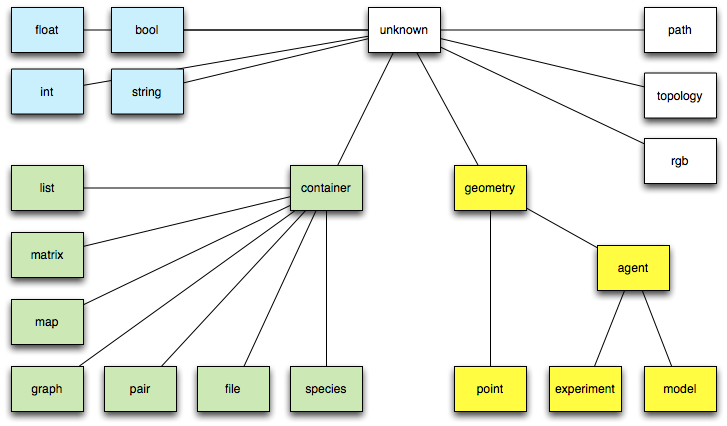
\includegraphics{resources/images/gamlReferences/types_hierarchy.png}
\caption{images/types\_hierarchy.png}
\end{figure}

\hypertarget{table-of-contents-1}{%
\section{Table of contents}\label{table-of-contents-1}}

\begin{itemize}
\tightlist
\item
  \protect\hyperlink{types-under-construction}{Types (Under
  Construction)}

  \begin{itemize}
  \tightlist
  \item
    \protect\hyperlink{primitive-built-in-types}{Primitive built-in
    types}

    \begin{itemize}
    \tightlist
    \item
      \protect\hyperlink{bool}{bool}
    \item
      \protect\hyperlink{float}{float}
    \item
      \protect\hyperlink{int}{int}
    \item
      \protect\hyperlink{string}{string}
    \end{itemize}
  \item
    \protect\hyperlink{complex-built-in-types}{Complex built-in types}

    \begin{itemize}
    \tightlist
    \item
      \protect\hyperlink{agent}{agent}
    \item
      \protect\hyperlink{container}{container}
    \item
      \protect\hyperlink{file}{file}
    \item
      \protect\hyperlink{geometry}{geometry}
    \item
      \protect\hyperlink{graph}{graph}
    \item
      \protect\hyperlink{list}{list}
    \item
      \protect\hyperlink{map}{map}
    \item
      \protect\hyperlink{matrix}{matrix}
    \item
      \protect\hyperlink{pair}{pair}
    \item
      \protect\hyperlink{path}{path}
    \item
      \protect\hyperlink{point}{point}
    \item
      \protect\hyperlink{rgb}{rgb}
    \item
      \protect\hyperlink{species}{species}
    \item
      \protect\hyperlink{species-names-as-types}{Species names as types}
    \item
      \protect\hyperlink{topology}{topology}
    \end{itemize}
  \item
    \protect\hyperlink{defining-custom-types}{Defining custom types}
  \end{itemize}
\end{itemize}

\hypertarget{primitive-built-in-types}{%
\section{Primitive built-in types}\label{primitive-built-in-types}}

\hypertarget{bool}{%
\subsection{bool}\label{bool}}

\begin{itemize}
\tightlist
\item
  \textbf{Definition:} primitive datatype providing two values:
  \texttt{true} or \texttt{false}.
\item
  \textbf{Litteral declaration:} both \texttt{true} or \texttt{false}
  are interpreted as boolean constants.
\item
  \textbf{Other declarations:} expressions that require a boolean
  operand often directly apply a casting to bool to their operand. It is
  a convenient way to directly obtain a bool value.
\end{itemize}

\begin{verbatim}
bool (0) -> false
\end{verbatim}

\protect\hyperlink{table-of-contents}{Top of the page}

\hypertarget{float}{%
\subsection{float}\label{float}}

\begin{itemize}
\tightlist
\item
  \textbf{Definition:} primitive datatype holding floating point values,
  its absolute value is comprised between 4.9E-324 and 1.8E308.
\item
  \textbf{Comments:} this datatype is internally backed up by the Java
  double datatype.
\item
  \textbf{Litteral declaration:} decimal notation 123.45 or exponential
  notation 123e45 are supported.
\item
  \textbf{Other declarations:} expressions that require an integer
  operand often directly apply a casting to float to their operand.
  Using it is a way to obtain a float constant.
\end{itemize}

\begin{verbatim}
float (12) -> 12.0
\end{verbatim}

\protect\hyperlink{table-of-contents}{Top of the page}

\hypertarget{int}{%
\subsection{int}\label{int}}

\begin{itemize}
\tightlist
\item
  \textbf{Definition:} primitive datatype holding integer values
  comprised between -2147483648 and 2147483647 (i.e.~between
  \texttt{-2\^{}31} and \texttt{2\^{}31\ -\ 1}.
\item
  \textbf{Comments:} this datatype is internally backed up by the Java
  int datatype.
\item
  \textbf{Litteral declaration:} decimal notation like 1, 256790 or
  hexadecimal notation like \#1209FF are automatically interpreted.
\item
  \textbf{Other declarations:} expressions that require an integer
  operand often directly apply a casting to int to their operand. Using
  it is a way to obtain an integer constant.
\end{itemize}

\begin{verbatim}
int (234.5) -> 234.
\end{verbatim}

\protect\hyperlink{table-of-contents}{Top of the page}

\hypertarget{string}{%
\subsection{string}\label{string}}

\begin{itemize}
\tightlist
\item
  \textbf{Definition:} a datatype holding a sequence of characters.
\item
  \textbf{Comments:} this datatype is internally backed up by the Java
  String class. However, contrary to Java, strings are considered as a
  primitive type, which means they do not contain character objects.
  This can be seen when casting a string to a list using the list
  operator: the result is a list of one-character strings, not a list of
  characters.
\item
  \textbf{Litteral declaration:} a sequence of characters enclosed in
  quotes, like `this is a string' . If one wants to literally declare
  strings that contain quotes, one has to double these quotes in the
  declaration. Strings accept escape characters like
  \texttt{\textbackslash{}n} (newline), \texttt{\textbackslash{}r}
  (carriage return), \texttt{\textbackslash{}t} (tabulation), as well as
  any Unicode character (\texttt{\textbackslash{}uXXXX}).
\item
  \textbf{Other declarations:} see string
\item
  \textbf{Example:} see
  \href{Operators\#strings-related-operators}{string operators}.
\end{itemize}

\protect\hyperlink{table-of-contents}{Top of the page}

\hypertarget{complex-built-in-types}{%
\section{Complex built-in types}\label{complex-built-in-types}}

Contrarily to primitive built-in types, complex types have often various
attributes. They can be accessed in the same way as attributes of
agents:

\begin{verbatim}
complex_type nom_var <- init_var;
ltype_attr attr_var <- nom_var.attr_name;
\end{verbatim}

For example:

\begin{verbatim}
file fileText <- file("../data/cell.Data");
bool fileTextReadable <- fileText.readable;
\end{verbatim}

\hypertarget{agent}{%
\subsection{agent}\label{agent}}

\begin{itemize}
\tightlist
\item
  \textbf{Definition:} a generic datatype that represents an agent
  whatever its actual species.
\item
  \textbf{Comments:} This datatype is barely used, since species can be
  directly used as datatypes themselves.
\item
  \textbf{Declaration:} the agent casting operator can be applied to an
  int (to get the agent with this unique index), a string (to get the
  agent with this name).
\end{itemize}

\protect\hyperlink{table-of-contents}{Top of the page}

\hypertarget{container}{%
\subsection{container}\label{container}}

\begin{itemize}
\tightlist
\item
  \textbf{Definition:} a generic datatype that represents a collection
  of data.
\item
  \textbf{Comments:} a container variable can be a list, a matrix, a
  map\ldots{} Conversely each list, matrix and map is a kind of
  container. In consequence every container can be used in
  container-related operators.
\item
  \textbf{See also:}
  \href{Operators\#containers-related-operators}{Container operators}
\item
  \textbf{Declaration:}
\end{itemize}

\begin{verbatim}
container c  <- [1,2,3];
container c  <- matrix [[1,2,3],[4,5,6]];
container c  <- map ["x"::5, "y"::12];
container c  <- list species1;
\end{verbatim}

\protect\hyperlink{table-of-contents}{Top of the page}

\hypertarget{file}{%
\subsection{file}\label{file}}

\begin{itemize}
\tightlist
\item
  \textbf{Definition:} a datatype that represents a file.
\item
  \textbf{Built-in attributes:}

  \begin{itemize}
  \tightlist
  \item
    name (type = string): the name of the represented file (with its
    extension)
  \item
    extension(type = string): the extension of the file
  \item
    path (type = string): the absolute path of the file
  \item
    readable (type = bool, read-only): a flag expressing whether the
    file is readable
  \item
    writable (type = bool, read-only): a flag expressing whether the
    file is writable
  \item
    exists (type = bool, read-only): a flag expressing whether the file
    exists
  \item
    is\_folder (type = bool, read-only): a flag expressing whether the
    file is folder
  \item
    contents (type = container): a container storing the content of the
    file
  \end{itemize}
\item
  \textbf{Comments:} a variable with the \texttt{file} type can handle
  any kind of file (text, image or shape files\ldots{}). The type of the
  \texttt{content} attribute will depend on the kind of file. Note that
  the allowed kinds of file are the followings:

  \begin{itemize}
  \tightlist
  \item
    text files: files with the extensions .txt, .data, .csv, .text,
    .tsv, .asc. The \texttt{content} is by default a list of string.
  \item
    image files: files with the extensions .pgm, .tif, .tiff, .jpg,
    .jpeg, .png, .gif, .pict, .bmp. The \texttt{content} is by default a
    matrix of int.
  \item
    shapefiles: files with the extension .shp. The \texttt{content} is
    by default a list of geometry.
  \item
    properties files: files with the extension .properties. The
    \texttt{content} is by default a map of string::string.
  \item
    folders. The \texttt{content} is by default a list of string.
  \end{itemize}
\item
  \textbf{Remark:} Files are also a particular kind of container and can
  thus be read, written or iterated using the container operators and
  commands.
\item
  \textbf{See also:} \href{Operators\#files-related-operators}{File
  operators}
\item
  \textbf{Declaration:} a file can be created using the generic
  \texttt{file} (that opens a file in read only mode and tries to
  determine its contents), \texttt{folder} or the \texttt{new\_folder}
  (to open an existing folder or create a new one) unary operators. But
  things can be specialized with the combination of the
  \texttt{read}/\texttt{write} and
  \texttt{image}/\texttt{text}/\texttt{shapefile}/\texttt{properties}
  unary operators.
\end{itemize}

\begin{verbatim}
folder(a_string)  // returns a file managing a existing folder
file(a_string) // returns any kind of file in read-only mode
read(text(a_string)) // returns a text file in read-only mode
read(image(a_string)) // does the same with an image file.
write(properties(a_string)) // returns a property file which is available for writing 
                            // (if it exists, contents will be appended unless it is cleared 
                            // using the standard container operations).
\end{verbatim}

\protect\hyperlink{table-of-contents}{Top of the page}

\hypertarget{geometry}{%
\subsection{geometry}\label{geometry}}

\begin{itemize}
\tightlist
\item
  \textbf{Definition:} a datatype that represents a vector geometry,
  i.e.~a list of georeferenced points.
\item
  \textbf{Built-in attributes:}

  \begin{itemize}
  \tightlist
  \item
    location (type = point): the centroid of the geometry
  \item
    area (type = float): the area of the geometry
  \item
    perimeter (type = float): the perimeter of the geometry
  \item
    holes (type = list of geometry): the list of the hole inside the
    given geometry
  \item
    contour (type = geometry): the exterior ring of the given geometry
    and of his holes
  \item
    envelope (type = geometry): the geometry bounding box
  \item
    width (type = float): the width of the bounding box
  \item
    height (type = float): the height of the bounding box
  \item
    points (type = list of point): the set of the points composing the
    geometry
  \end{itemize}
\item
  \textbf{Comments:} a geometry can be either a point, a polyline or a
  polygon. Operators working on geometries handle transparently these
  three kinds of geometry. The envelope (a.k.a. the bounding box) of the
  geometry depends on the kind of geometry:

  \begin{itemize}
  \tightlist
  \item
    If this Geometry is the empty geometry, it is an empty point.
  \item
    If the Geometry is a point, it is a non-empty point.
  \item
    Otherwise, it is a Polygon whose points are (minx, miny), (maxx,
    miny), (maxx, maxy), (minx, maxy), (minx, miny).
  \end{itemize}
\item
  \textbf{See also:} \href{Operators\#spatial-operators}{Spatial
  operators}
\item
  \textbf{Declaration:} geometries can be built from a point, a list of
  points or by using specific operators (circle, square,
  triangle\ldots{}).
\end{itemize}

\begin{verbatim}
geometry varGeom <- circle(5);
geometry polygonGeom <- polygon([{3,5}, {5,6},{1,4}]);
\end{verbatim}

\protect\hyperlink{table-of-contents}{Top of the page}

\hypertarget{graph}{%
\subsection{graph}\label{graph}}

\begin{itemize}
\tightlist
\item
  \textbf{Definition:} a datatype that represents a graph composed of
  vertices linked by edges.
\item
  \textbf{Built-in attributes:}

  \begin{itemize}
  \tightlist
  \item
    edges(type = list of agent/geometry): the list of all edges
  \item
    vertices(type = list of agent/geometry): the list of all vertices
  \item
    circuit (type = path): an approximate minimal traveling salesman
    tour (hamiltonian cycle)
  \item
    spanning\_tree (type = list of agent/geometry): minimum spanning
    tree of the graph, i.e.~a sub-graph such as every vertex lies in the
    tree, and as much edges lies in it but no cycles (or loops) are
    formed.
  \item
    connected(type = bool): test whether the graph is connected
  \end{itemize}
\item
  \textbf{Remark:}

  \begin{itemize}
  \tightlist
  \item
    graphs are also a particular kind of container and can thus be
    manipulated using the container operators and commands.
  \item
    This algorithm used to compute the circuit requires that the graph
    be complete and the triangle inequality exists (if x,y,z are
    vertices then d(x,y)+d(y,z)\textless{}d(x,z) for all x,y,z) then
    this algorithm will guarantee a hamiltonian cycle such that the
    total weight of the cycle is less than or equal to double the total
    weight of the optimal hamiltonian cycle.
  \item
    The computation of the spanning tree uses an implementation of the
    Kruskal's minimum spanning tree algorithm. If the given graph is
    connected it computes the minimum spanning tree, otherwise it
    computes the minimum spanning forest.
  \end{itemize}
\item
  \textbf{See also:} \href{Operators\#graph-related-operators}{Graph
  operators}
\item
  \textbf{Declaration:} graphs can be built from a list of vertices
  (agents or geometries) or from a list of edges (agents or geometries)
  by using specific operators. They are often used to deal with a road
  network and are built from a shapefile.
\end{itemize}

\begin{verbatim}
create road from: shape_file_road;
graph the_graph <- as_edge_graph(road);

graph([1,9,5])        --: ([1: in[] + out[], 5: in[] + out[], 9: in[] + out[]], [])
graph([node(0), node(1), node(2)]      // if node is a species
graph(['a'::345, 'b'::13])  --:  ([b: in[] + out[b::13], a: in[] + out[a::345], 13: in[b::13] + out[], 345: in[a::345] + out[]], [a::345=(a,345), b::13=(b,13)])
graph(a_graph)  --: a_graph
graph(node1)    --: null
\end{verbatim}

\protect\hyperlink{table-of-contents}{Top of the page}

\hypertarget{list}{%
\subsection{list}\label{list}}

\begin{itemize}
\tightlist
\item
  \textbf{Definition:} a composite datatype holding an ordered
  collection of values.
\item
  \textbf{Comments:} lists are more or less equivalent to instances of
  ArrayList in Java (although they are backed up by a specific class).
  They grow and shrink as needed, can be accessed via an index (see @ or
  index\_of), support set operations (like union and difference), and
  provide the modeller with a number of utilities that make it easy to
  deal with collections of agents (see, for instance, shuffle,
  reverse,where,sort\_by,\ldots{}).
\item
  \textbf{Remark:} lists can contain values of any datatypes, including
  other lists. Note, however, that due to limitations in the current
  parser, lists of lists cannot be declared litteraly; they have to be
  built using assignments. Lists are also a particular kind of container
  and can thus be manipulated using the container operators and
  commands.
\item
  \textbf{Litteral declaration:} a set of expressions separated by
  commas, enclosed in square brackets, like {[}12, 14, `abc', self{]}.
  An empty list is noted \href{}{}.
\item
  \textbf{Other declarations:} lists can be build litteraly from a
  point, or a string, or any other element by using the list casting
  operator.
\end{itemize}

\begin{verbatim}
list (1) -> [1]
\end{verbatim}

\begin{verbatim}
list<int> myList <- [1,2,3,4]; 
myList[2] => 3
\end{verbatim}

\protect\hyperlink{table-of-contents}{Top of the page}

\hypertarget{map}{%
\subsection{map}\label{map}}

\begin{itemize}
\tightlist
\item
  \textbf{Definition:} a composite datatype holding an ordered
  collection of pairs (a key, and its associated value).
\item
  \textbf{Built-in attributes:}

  \begin{itemize}
  \tightlist
  \item
    keys (type = list): the list of all keys
  \item
    values (type = list): the list of all values
  \item
    pairs (type = list of pairs): the list of all pairs key::value
  \end{itemize}
\item
  \textbf{Comments:} maps are more or less equivalent to instances of
  Hashtable in Java (although they are backed up by a specific class).
\item
  \textbf{Remark:} maps can contain values of any datatypes, including
  other maps or lists. Maps are also a particular kind of container and
  can thus be manipulated using the container operators and commands.
\item
  \textbf{Litteral declaration:} a set of pair expressions separated by
  commas, enclosed in square brackets; each pair is represented by a key
  and a value sperarated by `::'. An example of map is {[}agentA::`big',
  agentB::`small', agentC::`big'{]}. An empty map is noted \href{}{}.
\item
  \textbf{Other declarations:} lists can be built litteraly from a
  point, or a string, or any other element by using the map casting
  operator.
\end{itemize}

\begin{verbatim}
map (1) -> [1::1]
map ({1,5}) -> [x::1, y::5]
[]   // empty map 
\end{verbatim}

\protect\hyperlink{table-of-contents}{Top of the page}

\hypertarget{matrix}{%
\subsection{matrix}\label{matrix}}

\begin{itemize}
\tightlist
\item
  \textbf{Definition:} a composite datatype that represents either a
  two-dimension array (matrix) or a one-dimension array (vector),
  holding any type of data (including other matrices).
\item
  \textbf{Comments:} Matrices are fixed-size structures that can be
  accessed by index (point for two-dimensions matrices, integer for
  vectors).
\item
  \textbf{Litteral declaration:} Matrices cannot be defined literally.
  One-dimensions matrices can be built by using the matrix casting
  operator applied on a list. Two-dimensions matrices need to to be
  declared as variables first, before being filled.
\end{itemize}

\begin{verbatim}
//builds a one-dimension matrix, of size 5
matrix mat1 <- matrix ([10, 20, 30, 40, 50]);
//  builds a two-dimensions matrix with 10 columns and 5 rows, where each cell is initialized to 0.0
matrix mat2 <- 0.0 as_matrix({10,5}); 
// builds a two-dimensions matrix with 2 columns and 3 rows, with initialized cells
matrix mat3 <- matrix([["c11","c12","c13"],["c21","c22","c23"]]);     
    -> c11;c21
       c12;c22
       c13;c23
\end{verbatim}

\protect\hyperlink{table-of-contents}{Top of the page}

\hypertarget{pair}{%
\subsection{pair}\label{pair}}

\begin{itemize}
\tightlist
\item
  \textbf{Definition:} a datatype holding a key and its associated
  value.
\item
  \textbf{Built-in attributes:}

  \begin{itemize}
  \tightlist
  \item
    key (type = string): the key of the pair, i.e.~the first element of
    the pair
  \item
    value (type = string): the value of the pair, i.e.~the second
    element of the pair
  \end{itemize}
\item
  \textbf{Remark:} pairs are also a particular kind of container and can
  thus be manipulated using the container operators and commands.
\item
  \textbf{Litteral declaration:} a pair is defined by a key and a value
  sperarated by `::'.
\item
  \textbf{Other declarations:} a pair can also be built from:

  \begin{itemize}
  \tightlist
  \item
    a point,
  \item
    a map (in this case the first element of the pair is the list of all
    the keys of the map and the second element is the list of all the
    values of the map),
  \item
    a list (in this case the two first element of the list are used to
    built the pair)
  \end{itemize}
\end{itemize}

\begin{verbatim}
pair testPair <- "key"::56;
pair testPairPoint <- {3,5};             // 3::5
pair testPairList2 <- [6,7,8];           // 6::7
pair testPairMap <- [2::6,5::8,12::45];  // [12,5,2]::[45,8,6]
\end{verbatim}

\protect\hyperlink{table-of-contents}{Top of the page}

\hypertarget{path}{%
\subsection{path}\label{path}}

\begin{itemize}
\tightlist
\item
  \textbf{Definition:} a datatype representing a path linking two agents
  or geometries in a graph.
\item
  \textbf{Built-in attributes:}

  \begin{itemize}
  \tightlist
  \item
    source (type = point): the source point, i.e.~the first point of the
    path
  \item
    target (type = point): the target point, i.e.~the last point of the
    path
  \item
    graph (type = graph): the current topology (in the case it is a
    spatial graph), null otherwise
  \item
    edges (type = list of agents/geometries) : the edges of the graph
    composing the path
  \item
    vertices (type = list of agents/geometries) : the vertices of the
    graph composing the path
  \item
    segments (type = list of geometries): the list of the geometries
    composing the path
  \item
    shape (type = geometry) : the global geometry of the path (polyline)
  \end{itemize}
\item
  \textbf{Comments:} the path created between two agents/geometries or
  locations will strongly depends on the topology in which it is
  created.
\item
  \textbf{Remark:} a path is \textbf{immutable}, i.e.~it can not be
  modified after it is created.
\item
  \textbf{Declaration:} paths are very barely defined litterally. We can
  nevertheless use the \texttt{path} unary operator on a list of points
  to build a path. Operators dedicated to the computation of paths (such
  as path\_to or path\_between) are often used to build a path.
\end{itemize}

\begin{verbatim}
path([{1,5},{2,9},{5,8}]) // a path from {1,5} to {5,8} through {2,9}
       
geometry rect <- rectangle(5);
geometry poly <- polygon([{10,20},{11,21},{10,21},{11,22}]);
path pa <- rect path_to poly;  // built a path between rect and poly, in the topolopy   
                                            // of the current agent (i.e. a line in a& continuous topology, 
                                            // a path in a graph  in a graph topology )

a_topology path_between a_container_of_geometries // idem with an explicit topology and the possiblity 
                                                  // to have more than 2 geometries 
                                                  // (the path is then built incrementally)


path_between (a_graph, a_source, a_target) // idem with a the given graph as topology
\end{verbatim}

\protect\hyperlink{table-of-contents}{Top of the page}

\hypertarget{point}{%
\subsection{point}\label{point}}

\begin{itemize}
\tightlist
\item
  \textbf{Definition:} a datatype normally holding two positive float
  values. Represents the absolute coordinates of agents in the model.
\item
  \textbf{Built-in attributes:}

  \begin{itemize}
  \tightlist
  \item
    x (type = float): coordinate of the point on the x-axis
  \item
    y (type = float): coordinate of the point on the y-axis
  \end{itemize}
\item
  \textbf{Comments:} point coordinates should be positive, if a negative
  value is used in its declaration, the point is built with the absolute
  value.
\item
  \textbf{Remark:} points are particular cases of geometries and
  containers. Thus they have also all the built-in attributes of both
  the geometry and the container datatypes and can be used with every
  kind of operator or command admitting geometry and container.
\item
  \textbf{Litteral declaration:} two numbers, separated by a comma,
  enclosed in braces, like \{12.3, 14.5\}
\item
  \textbf{Other declarations:} points can be built litteraly from a
  list, or from an integer or float value by using the point casting
  operator.
\end{itemize}

\begin{verbatim}
point ([12,123.45]) -> {12.0, 123.45} 
point (2) -> {2.0, 2.0}
\end{verbatim}

\protect\hyperlink{table-of-contents}{Top of the page}

\hypertarget{rgb}{%
\subsection{rgb}\label{rgb}}

\begin{itemize}
\tightlist
\item
  \textbf{Definition:} a datatype that represents a color in the RGB
  space.
\item
  \textbf{Built-in attributes:}

  \begin{itemize}
  \tightlist
  \item
    red(type = int): the red component of the color
  \item
    green(type = int): the green component of the color
  \item
    blue(type = int): the blue component of the color
  \item
    darker(type = rgb): a new color that is a darker version of this
    color
  \item
    brighter(type = rgb): a new color that is a brighter version of this
    color
  \end{itemize}
\item
  \textbf{Remark:} rgbs are also a particular kind of container and can
  thus be manipulated using the container operators and commands.
\item
  \textbf{Litteral declaration:} there exist lot of ways to declare a
  color. We use the \texttt{rgb} casting operator applied to:

  \begin{itemize}
  \tightlist
  \item
    a string. The allowed color names are the constants defined in the
    Color Java class, i.e.: black, blue, cyan, darkGray, lightGray,
    gray, green, magenta, orange, pink, red, white, yellow.
  \item
    a list. The integer value associated to the three first elements of
    the list are used to define the three red (element 0 of the list),
    green (element 1 of the list) and blue (element 2 of the list)
    components of the color.
  \item
    a map. The red, green, blue compoenents take the value associated to
    the keys ``r'', ``g'', ``b'' in the map.
  \item
    an integer \textless{}- the decimal integer is translated into a
    hexadecimal \textless{}- OxRRGGBB. The red (resp. green, blue)
    component of the color take the value RR (resp. GG, BB) translated
    in decimal.
  \item
    Since GAMA 1.6.1, colors can be directly obtained like units, by
    using the ° or \# symbol followed by the name in lowercase of one of
    the 147 CSS colors (see
    \url{http://www.cssportal.com/css3-color-names/}).
  \end{itemize}
\item
  \textbf{Declaration:}
\end{itemize}

\begin{verbatim}
rgb cssRed <- #red;   // Since 1.6.1
rgb testColor <- rgb('white');                 // rgb [255,255,255]
rgb test <- rgb(3,5,67);                     // rgb [3,5,67]
rgb te <- rgb(340);                            // rgb [0,1,84]
rgb tete <- rgb(["r"::34, "g"::56, "b"::345]); // rgb [34,56,255]
\end{verbatim}

\protect\hyperlink{table-of-contents}{Top of the page}

\hypertarget{species}{%
\subsection{species}\label{species}}

\begin{itemize}
\tightlist
\item
  Definition: a generic datatype that represents a species
\item
  \textbf{Built-in attributes:}

  \begin{itemize}
  \tightlist
  \item
    topology (type=topology): the topology is which lives the population
    of agents
  \end{itemize}
\item
  Comments: this datatype is actually a ``meta-type''. It allows to
  manipulate (in a rather limited fashion, however) the species
  themselves as any other values.
\item
  Litteral declaration: the name of a declared species is already a
  litteral declaration of species.
\item
  Other declarations: the species casting operator, or its variant
  called species\_of can be applied to an agent in order to get its
  species.
\end{itemize}

\protect\hyperlink{table-of-contents}{Top of the page}

\hypertarget{species-names-as-types}{%
\subsection{Species names as types}\label{species-names-as-types}}

Once a species has been declared in a model, it automatically becomes a
datatype. This means that : * It can be used to declare variables,
parameters or constants, * It can be used as an operand to commands or
operators that require species parameters, * It can be used as a casting
operator (with the same capabilities as the built-in type agent)

In the simple following example, we create a set of ``humans'' and
initialize a random ``friendship network'' among them. See how the name
of the species, human, is used in the create command, as an argument to
the list casting operator, and as the type of the variable named friend.

\begin{verbatim}
global {
    init {
         create human number: 10;
         ask human {
               friend <- one_of (human - self);
         }
     }
}
entities {
    species human {
        human friend <- nil;
    }
}
\end{verbatim}

\protect\hyperlink{table-of-contents}{Top of the page}

\hypertarget{topology}{%
\subsection{topology}\label{topology}}

\begin{itemize}
\tightlist
\item
  \textbf{Definition:} a topology is basically on neighborhoods,
  distance,\ldots{} structures in which agents evolves. It is the
  environment or the context in which all these values are computed. It
  also provides the access to the spatial index shared by all the
  agents. And it maintains a (eventually dynamic) link with the
  `environment' which is a geometrical border.
\item
  \textbf{Built-in attributes:}

  \begin{itemize}
  \tightlist
  \item
    places(type = container): the collection of places (geometry)
    defined by this topology.
  \item
    environment(type = geometry): the environment of this topology
    (i.e.~the geometry that defines its boundaries)
  \end{itemize}
\item
  \textbf{Comments:} the attributes \texttt{places} depends on the kind
  of the considered topolopy. For continuous topologies, it is a list
  with their environment. For discrete topologies, it can be any of the
  container supporting the inclusion of geometries (list, graph, map,
  matrix)
\item
  \textbf{Remark:} There exist various kinds of topology: continuous
  topology and discrete topology (e.g.~grid, graph\ldots{})
\item
  \textbf{Declaration:} To create a topology, we can use the
  \texttt{topology} unary casting operator applied to:

  \begin{itemize}
  \tightlist
  \item
    an agent: returns a continuous topology built from the agent's
    geometry
  \item
    a species name: returns the topology defined for this species
    population
  \item
    a geometry: returns a continuous topology built on this geometry
  \item
    a geometry container (list, map, shapefile): returns an
    half-discrete (with corresponding places), half-continuous topology
    (to compute distances\ldots{})
  \item
    a geometry matrix (i.e.~a grid): returns a grid topology which
    computes specifically neighborhood and distances
  \item
    a geometry graph: returns a graph topology which computes
    specifically neighborhood and distances More complex topologies can
    also be built using dedicated operators, e.g.~to decompose a
    geometry\ldots{}
  \end{itemize}
\end{itemize}

\protect\hyperlink{table-of-contents}{Top of the page}

\hypertarget{defining-custom-types}{%
\section{Defining custom types}\label{defining-custom-types}}

Sometimes, besides the species of agents that compose the model, it can
be necessary to declare custom datatypes. Species serve this purpose as
well, and can be seen as ``classes'' that can help to instantiate simple
``objects''. In the following example, we declare a new kind of
``object'', bottle, that lacks the skills habitually associated with
agents (moving, visible, etc.), but can nevertheless group together
attributes and behaviors within the same closure. The following example
demonstrates how to create the species:

\begin{verbatim}
species bottle {
    float volume <- 0.0 max:1 min:0.0;
    bool is_empty -> {volume = 0.0};
    action fill {
         volume <- 1.0;
    }
}
\end{verbatim}

How to use this species to declare new bottles :

\begin{verbatim}
create bottle {
    volume <- 0.5;
}
\end{verbatim}

And how to use bottles as any other agent in a species (a drinker owns a
bottle; when he gets thirsty, it drinks a random quantity from it; when
it is empty, it refills it):

\begin{verbatim}
species drinker {
     ...
    bottle my_bottle<- nil;
    float quantity <- rnd (100) / 100;
    bool thirsty <- false update: flip (0.1);
    ...
    action drink {
         if condition: ! bottle.is_empty {
              bottle.volume <-bottle.volume - quantity;
              thirsty <- false;
         }
    }
    ...
    init {
          create bottle return: created_bottle;
              volume <- 0.5;
          }
          my_bottle <- first(created_bottle);
    }
    ...
    reflex filling_bottle when: bottle.is_empty {
         ask  my_bottle {
              do fill;
         }
    }
    ...
    reflex drinking when: thirsty {
         do drink;
    }
}
\end{verbatim}

\protect\hyperlink{table-of-contents}{Top of the page}

\hypertarget{file-types}{%
\chapter{File Types}\label{file-types}}

GAMA provides modelers with a generic type for files called
\textbf{file}. It is possible to load a file using the \emph{file}
operator:

\begin{verbatim}
file my_file <- file("../includes/data.csv");
\end{verbatim}

However, internally, GAMA makes the difference between the different
types of files. Indeed, for instance:

\begin{verbatim}
global {
    init {
        file my_file <- file("../includes/data.csv");
        loop el over: my_file {
            write el;
        }
    }
}
\end{verbatim}

will give:

\begin{verbatim}
sepallength
sepalwidth
petallength
petalwidth
type
5.1
3.5
1.4
0.2
Iris-setosa
4.9
3.0
1.4
0.2
Iris-setosa
...
\end{verbatim}

Indeed, the content of CSV file is a matrix: each row of the matrix is a
line of the file; each column of the matrix is value delimited by the
separator (by default ``,'').

In contrary:

\begin{verbatim}
global {
    init {
        file my_file <- file("../includes/data.shp");
        loop el over: my_file {
            write el;
        }
    }
}
\end{verbatim}

will give:

\begin{verbatim}
Polygon
Polygon
Polygon
Polygon
Polygon
Polygon
Polygon
\end{verbatim}

The content of a shapefile is a list of geometries corresponding to the
objects of the shapefile.

In order to know how to load a file, GAMA analyzes its extension. For
instance for a file with a ``.csv'' extension, GAMA knows that the file
is a \textbf{csv} one and will try to split each line with the \emph{,}
separator. However, if the modeler wants to split each line with a
different separator (for instance \textbf{;}) or load it as a text file,
he/she will have to use a specific file operator.

Indeed, GAMA integrates specific operators corresponding to different
types of files.

\hypertarget{table-of-contents-2}{%
\section{Table of contents}\label{table-of-contents-2}}

\begin{itemize}
\tightlist
\item
  \protect\hyperlink{file-types}{File Types}

  \begin{itemize}
  \tightlist
  \item
    \protect\hyperlink{text-file}{Text File}

    \begin{itemize}
    \tightlist
    \item
      \protect\hyperlink{extensions}{Extensions}
    \item
      \protect\hyperlink{content}{Content}
    \item
      \protect\hyperlink{operators}{Operators}
    \end{itemize}
  \item
    \protect\hyperlink{csv-file}{CSV File}

    \begin{itemize}
    \tightlist
    \item
      \protect\hyperlink{extensions}{Extensions}
    \item
      \protect\hyperlink{content}{Content}
    \item
      \protect\hyperlink{operators}{Operators}
    \end{itemize}
  \item
    \protect\hyperlink{shapefile}{Shapefile}

    \begin{itemize}
    \tightlist
    \item
      \protect\hyperlink{extensions}{Extensions}
    \item
      \protect\hyperlink{content}{Content}
    \item
      \protect\hyperlink{operators}{Operators}
    \end{itemize}
  \item
    \protect\hyperlink{osm-file}{OSM File}

    \begin{itemize}
    \tightlist
    \item
      \protect\hyperlink{extensions}{Extensions}
    \item
      \protect\hyperlink{content}{Content}
    \item
      \protect\hyperlink{operators}{Operators}
    \end{itemize}
  \item
    \protect\hyperlink{grid-file}{Grid File}

    \begin{itemize}
    \tightlist
    \item
      \protect\hyperlink{extensions}{Extensions}
    \item
      \protect\hyperlink{content}{Content}
    \item
      \protect\hyperlink{operators}{Operators}
    \end{itemize}
  \item
    \protect\hyperlink{image-file}{Image File}

    \begin{itemize}
    \tightlist
    \item
      \protect\hyperlink{extensions}{Extensions}
    \item
      \protect\hyperlink{content}{Content}
    \item
      \protect\hyperlink{operators}{Operators}
    \end{itemize}
  \item
    \protect\hyperlink{svg-file}{SVG File}

    \begin{itemize}
    \tightlist
    \item
      \protect\hyperlink{extensions}{Extensions}
    \item
      \protect\hyperlink{content}{Content}
    \item
      \protect\hyperlink{operators}{Operators}
    \end{itemize}
  \item
    \protect\hyperlink{property-file}{Property File}

    \begin{itemize}
    \tightlist
    \item
      \protect\hyperlink{extensions}{Extensions}
    \item
      \protect\hyperlink{content}{Content}
    \item
      \protect\hyperlink{operators}{Operators}
    \end{itemize}
  \item
    \protect\hyperlink{r-file}{R File}

    \begin{itemize}
    \tightlist
    \item
      \protect\hyperlink{extensions}{Extensions}
    \item
      \protect\hyperlink{content}{Content}
    \item
      \protect\hyperlink{operators}{Operators}
    \end{itemize}
  \item
    \protect\hyperlink{3ds-file}{3DS File}

    \begin{itemize}
    \tightlist
    \item
      \protect\hyperlink{extensions}{Extensions}
    \item
      \protect\hyperlink{content}{Content}
    \item
      \protect\hyperlink{operators}{Operators}
    \end{itemize}
  \item
    \protect\hyperlink{obj-file}{OBJ File}

    \begin{itemize}
    \tightlist
    \item
      \protect\hyperlink{extensions}{Extensions}
    \item
      \protect\hyperlink{content}{Content}
    \item
      \protect\hyperlink{operators}{Operators}
    \end{itemize}
  \end{itemize}
\end{itemize}

\hypertarget{text-file}{%
\section{Text File}\label{text-file}}

\hypertarget{extensions}{%
\subsection{Extensions}\label{extensions}}

Here the list of possible extensions for text file: * ``txt'' * ``data''
* ``csv'' * ``text'' * ``tsv'' * ``xml''

Note that when trying to define the type of a file with the default file
loading operator (\textbf{file}), GAMA will first try to test the other
type of file. For example, for files with ``.csv'' extension, GAMA will
cast them as csv file and not as text file.

\hypertarget{content}{%
\subsection{Content}\label{content}}

The content of a text file is a list of string corresponding to each
line of the text file. For example:

\begin{verbatim}
global {
    init {
        file my_file <- text_file("../includes/data.txt");
        loop el over: my_file {
            write el;
        }
    }
}
\end{verbatim}

will give:

\begin{verbatim}
sepallength,sepalwidth,petallength,petalwidth,type
5.1,3.5,1.4,0.2,Iris-setosa
4.9,3.0,1.4,0.2,Iris-setosa
4.7,3.2,1.3,0.2,Iris-setosa
\end{verbatim}

\hypertarget{operators}{%
\subsection{Operators}\label{operators}}

List of operators related to text files: * \textbf{text\_file(string
path)}: load a file (with an authorized extension) as a text file. *
\textbf{text\_file(string path, list content)}: load a file (with an
authorized extension) as a text file and fill it with the given content.
* \textbf{is\_text(op)}: tests whether the operand is a text file

\hypertarget{csv-file}{%
\section{CSV File}\label{csv-file}}

\hypertarget{extensions-1}{%
\subsection{Extensions}\label{extensions-1}}

Here the list of possible extensions for csv file: * ``csv'' * ``tsv''

\hypertarget{content-1}{%
\subsection{Content}\label{content-1}}

The content of a csv file is a matrix of string: each row of the matrix
is a line of the file; each column of the matrix is value delimited by
the separator (by default ``,''). For example:

\begin{verbatim}
global {
    init {
        file my_file <- csv_file("../includes/data.csv");
        loop el over: my_file {
            write el;
        }
    }
}
\end{verbatim}

will give:

\begin{verbatim}
sepallength
sepalwidth
petallength
petalwidth
type
5.1
3.5
1.4
0.2
Iris-setosa
4.9
3.0
1.4
0.2
Iris-setosa
...
\end{verbatim}

\hypertarget{operators-1}{%
\subsection{Operators}\label{operators-1}}

List of operators related to csv files: * \textbf{csv\_file(string
path)}: load a file (with an authorized extension) as a csv file with
default separator (``,''). * \textbf{csv\_file(string path, string
separator)}: load a file (with an authorized extension) as a csv file
with the given separator.

\begin{verbatim}
file my_file <- csv_file("../includes/data.csv", ";");
\end{verbatim}

\begin{itemize}
\tightlist
\item
  \textbf{csv\_file(string path, matrix content)}: load a file (with an
  authorized extension) as a csv file and fill it with the given
  content.
\item
  \textbf{is\_csv(op)}: tests whether the operand is a csv file
\end{itemize}

\hypertarget{shapefile}{%
\section{Shapefile}\label{shapefile}}

Shapefiles are classical GIS data files. A shapefile is not simple file,
but a set of several files (source: wikipedia): * Mandatory files : *
.shp --- shape format; the feature geometry itself * .shx --- shape
index format; a positional index of the feature geometry to allow
seeking forwards and backwards quickly * .dbf --- attribute format;
columnar attributes for each shape, in dBase IV format

\begin{itemize}
\tightlist
\item
  Optional files :

  \begin{itemize}
  \tightlist
  \item
    .prj --- projection format; the coordinate system and projection
    information, a plain text file describing the projection using
    well-known text format
  \item
    .sbn and .sbx --- a spatial index of the features
  \item
    .fbn and .fbx --- a spatial index of the features for shapefiles
    that are read-only
  \item
    .ain and .aih --- an attribute index of the active fields in a table
  \item
    .ixs --- a geocoding index for read-write shapefiles
  \item
    .mxs --- a geocoding index for read-write shapefiles (ODB format)
  \item
    .atx --- an attribute index for the .dbf file in the form of
    shapefile.columnname.atx (ArcGIS 8 and later)
  \item
    .shp.xml --- geospatial metadata in XML format, such as ISO 19115 or
    other XML schema
  \item
    .cpg --- used to specify the code page (only for .dbf) for
    identifying the character encoding to be used
  \end{itemize}
\end{itemize}

More details about shapefiles can be found
\href{http://en.wikipedia.org/wiki/Shapefile}{here}.

\hypertarget{extensions-2}{%
\subsection{Extensions}\label{extensions-2}}

Here the list of possible extension for shapefile: * ``shp''

\hypertarget{content-2}{%
\subsection{Content}\label{content-2}}

The content of a shapefile is a list of geometries corresponding to the
objects of the shapefile. For example:

\begin{verbatim}
global {
    init {
        file my_file <- shape_file("../includes/data.shp");
        loop el over: my_file {
            write el;
        }
    }
}
\end{verbatim}

will give:

\begin{verbatim}
Polygon
Polygon
Polygon
Polygon
Polygon
Polygon
Polygon
...
\end{verbatim}

Note that the attributes of each object of the shapefile is stored in
their corresponding GAMA geometry. The operator ``get'' (or ``read'')
allows to get the value of a corresponding attributes.

For example:

\begin{verbatim}
file my_file <- shape_file("../includes/data.shp");
write "my_file: " + my_file.contents;
loop el over: my_file {
    write (el get "TYPE");
}
\end{verbatim}

\hypertarget{operators-2}{%
\subsection{Operators}\label{operators-2}}

List of operators related to shapefiles: * \textbf{shape\_file(string
path)}: load a file (with an authorized extension) as a shapefile with
default projection (if a prj file is defined, use it, otherwise use the
default projection defined in the preference). *
\textbf{shape\_file(string path, string code)}: load a file (with an
authorized extension) as a shapefile with the given projection (GAMA
will automatically decode the code. For a list of the possible
projections see: \url{http://spatialreference.org/ref/}) *
\textbf{shape\_file(string path, int EPSG\_ID)}: load a file (with an
authorized extension) as a shapefile with the given projection (GAMA
will automatically decode the epsg code. For a list of the possible
projections see: \url{http://spatialreference.org/ref/})

\begin{verbatim}
file my_file <- shape_file("../includes/data.shp", "EPSG:32601");
\end{verbatim}

\begin{itemize}
\tightlist
\item
  \textbf{shape\_file(string path, list content)}: load a file (with an
  authorized extension) as a shapefile and fill it with the given
  content.
\item
  \textbf{is\_shape(op)}: tests whether the operand is a shapefile
\end{itemize}

\hypertarget{osm-file}{%
\section{OSM File}\label{osm-file}}

OSM (Open Street Map) is a collaborative project to create a free
editable map of the world. The data produced in this project (OSM File)
represent physical features on the ground (e.g., roads or buildings)
using tags attached to its basic data structures (its nodes, ways, and
relations). Each tag describes a geographic attribute of the feature
being shown by that specific node, way or relation (source:
openstreetmap.org).

More details about OSM data can be found
\href{http://wiki.openstreetmap.org/wiki/Map_Features}{here}.

\hypertarget{extensions-3}{%
\subsection{Extensions}\label{extensions-3}}

Here the list of possible extension for shapefile: * ``osm'' * ``pbf'' *
``bz2'' * ``gz''

\hypertarget{content-3}{%
\subsection{Content}\label{content-3}}

The content of a OSM data is a list of geometries corresponding to the
objects of the OSM file. For example:

\begin{verbatim}
global {
    init {
        file my_file <- osm_file("../includes/data.gz");
        loop el over: my_file {
            write el;
        }
    }
}
\end{verbatim}

will give:

\begin{verbatim}
Point
Point
Point
Point
Point
LineString
LineString
Polygon
Polygon
Polygon
...
\end{verbatim}

Note that like for shapefiles, the attributes of each object of the osm
file is stored in their corresponding GAMA geometry. The operator
``get'' (or ``read'') allows to get the value of a corresponding
attributes.

\hypertarget{operators-3}{%
\subsection{Operators}\label{operators-3}}

List of operators related to osm file: * \textbf{osm\_file(string
path)}: load a file (with an authorized extension) as a osm file with
default projection (if a prj file is defined, use it, otherwise use the
default projection defined in the preference). In this case, all the
nodes and ways of the OSM file will becomes a geometry. *
\textbf{osm\_file(string path, string code)}: load a file (with an
authorized extension) as a osm file with the given projection (GAMA will
automatically decode the code. For a list of the possible projections
see: \url{http://spatialreference.org/ref/}). In this case, all the
nodes and ways of the OSM file will becomes a geometry. *
\textbf{osm\_file(string path, int EPSG\_ID)}: load a file (with an
authorized extension) as a osm file with the given projection (GAMA will
automatically decode the epsg code. For a list of the possible
projections see: \url{http://spatialreference.org/ref/}). In this case,
all the nodes and ways of the OSM file will becomes a geometry.

\begin{verbatim}
file my_file <- osm_file("../includes/data.gz", "EPSG:32601");
\end{verbatim}

\begin{itemize}
\tightlist
\item
  \textbf{osm\_file(string path, map filter)}: load a file (with an
  authorized extension) as a osm file with default projection (if a prj
  file is defined, use it, otherwise use the default projection defined
  in the preference). In this case, only the elements with the defined
  values are loaded from the file.
\end{itemize}

\begin{verbatim}
//map used to filter the object to build from the OSM file according to attributes. 
map filtering <- map(["highway"::["primary", "secondary", "tertiary", "motorway", "living_street","residential", "unclassified"], "building"::["yes"]]);

//OSM file to load
file<geometry> osmfile <-  file<geometry (osm_file("../includes/rouen.gz", filtering))  ;
\end{verbatim}

\begin{itemize}
\tightlist
\item
  \textbf{osm\_file(string path, map filter, string code)}: load a file
  (with an authorized extension) as a osm file with the given projection
  (GAMA will automatically decode the code. For a list of the possible
  projections see: \url{http://spatialreference.org/ref/}). In this
  case, only the elements with the defined values are loaded from the
  file.
\item
  \textbf{osm\_file(string path, map filter, int EPSG\_ID)}: load a file
  (with an authorized extension) as a osm file with the given projection
  (GAMA will automatically decode the epsg code. For a list of the
  possible projections see: \url{http://spatialreference.org/ref/}). In
  this case, only the elements with the defined values are loaded from
  the file.
\item
  \textbf{is\_osm(op)}: tests whether the operand is a osm file
\end{itemize}

\hypertarget{grid-file}{%
\section{Grid File}\label{grid-file}}

Esri ASCII Grid files are classic text raster GIS data.

More details about Esri ASCII grid file can be found
\href{http://en.wikipedia.org/wiki/Esri_grid}{here}.

Note that grid files can be used to initialize a grid species. The
number of rows and columns will be read from the file. Similarly, the
values of each cell contained in the grid file will be accessible
through the \textbf{grid\_value} attribute.

\begin{verbatim}
grid cell file: grid_file {
}
\end{verbatim}

\hypertarget{extensions-4}{%
\subsection{Extensions}\label{extensions-4}}

Here the list of possible extension for grid file: * ``asc''

\hypertarget{content-4}{%
\subsection{Content}\label{content-4}}

The content of a grid file is a list of geometries corresponding to the
cells of the grid. For example:

\begin{verbatim}
global {
    init {
        file my_file <- grid_file("../includes/data.asc");
        loop el over: my_file {
            write el;
        }
    }
}
\end{verbatim}

will give:

\begin{verbatim}
Polygon
Polygon
Polygon
Polygon
Polygon
Polygon
Polygon
...
\end{verbatim}

Note that the values of each cell of the grid file is stored in their
corresponding GAMA geometry (\textbf{grid\_value} attribute). The
operator ``get'' (or ``read'') allows to get the value of this
attribute.

For example:

\begin{verbatim}
file my_file <- grid_file("../includes/data.asc");
write "my_file: " + my_file.contents;
loop el over: my_file {
    write el get "grid_value";
}
\end{verbatim}

\hypertarget{operators-4}{%
\subsection{Operators}\label{operators-4}}

List of operators related to shapefiles: * \textbf{grid\_file(string
path)}: load a file (with an authorized extension) as a grid file with
default projection (if a prj file is defined, use it, otherwise use the
default projection defined in the preference). *
\textbf{grid\_file(string path, string code)}: load a file (with an
authorized extension) as a grid file with the given projection (GAMA
will automatically decode the code. For a list of the possible
projections see: \url{http://spatialreference.org/ref/}) *
\textbf{grid\_file(string path, int EPSG\_ID)}: load a file (with an
authorized extension) as a grid file with the given projection (GAMA
will automatically decode the epsg code. For a list of the possible
projections see: \url{http://spatialreference.org/ref/})

\begin{verbatim}
file my_file <- grid_file("../includes/data.shp", "EPSG:32601");
\end{verbatim}

\begin{itemize}
\tightlist
\item
  \textbf{is\_grid(op)}: tests whether the operand is a grid file.
\end{itemize}

\hypertarget{image-file}{%
\section{Image File}\label{image-file}}

\hypertarget{extensions-5}{%
\subsection{Extensions}\label{extensions-5}}

Here the list of possible extensions for image file: * ``tif'' *
``tiff'' * ``jpg'' * ``jpeg'' * ``png'' * ``gif'' * ``pict'' * ``bmp''

\hypertarget{content-5}{%
\subsection{Content}\label{content-5}}

The content of an image file is a matrix of int: each pixel is a value
in the matrix.

For example:

\begin{verbatim}
global {
    init {
        file my_file <- image_file("../includes/DEM.png");
        loop el over: my_file {
            write el;
        }
    }
}
\end{verbatim}

will give:

\begin{verbatim}
-9671572
-9671572
-9671572
-9671572
-9934744
-9934744
-9868951
-9868951
-10000537
-10000537
...
\end{verbatim}

\hypertarget{operators-5}{%
\subsection{Operators}\label{operators-5}}

List of operators related to csv files: * \textbf{image\_file(string
path)}: load a file (with an authorized extension) as an image file. *
\textbf{image\_file(string path, matrix content)}: load a file (with an
authorized extension) as an image file and fill it with the given
content. * \textbf{is\_image(op)}: tests whether the operand is an image
file

\hypertarget{svg-file}{%
\section{SVG File}\label{svg-file}}

Scalable Vector Graphics (SVG) is an XML-based vector image format for
two-dimensional graphics with support for interactivity and animation.
Note that interactivity and animation features are not supported in
GAMA.

More details about SVG file can be found
\href{http://en.wikipedia.org/wiki/Scalable_Vector_Graphics}{here}.

\hypertarget{extensions-6}{%
\subsection{Extensions}\label{extensions-6}}

Here the list of possible extension for SVG file: * ``svg''

\hypertarget{content-6}{%
\subsection{Content}\label{content-6}}

The content of a SVG file is a list of geometries. For example:

\begin{verbatim}
global {
    init {
        file my_file <- svg_file("../includes/data.svg");
        loop el over: my_file {
            write el;
        }
    }
}
\end{verbatim}

will give:

\begin{verbatim}
Polygon
\end{verbatim}

\hypertarget{operators-6}{%
\subsection{Operators}\label{operators-6}}

List of operators related to svg files: * \textbf{shape\_file(string
path)}: load a file (with an authorized extension) as a SVG file. *
\textbf{shape\_file(string path, point size)}: load a file (with an
authorized extension) as a SVG file with the given size:

\begin{verbatim}
file my_file <- svg_file("../includes/data.svg", {5.0,5.0});
\end{verbatim}

\begin{itemize}
\tightlist
\item
  \textbf{is\_svg(op)}: tests whether the operand is a SVG file
\end{itemize}

\hypertarget{property-file}{%
\section{Property File}\label{property-file}}

\hypertarget{extensions-7}{%
\subsection{Extensions}\label{extensions-7}}

Here the list of possible extensions for property file: * ``properties''

\hypertarget{content-7}{%
\subsection{Content}\label{content-7}}

The content of a property file is a map of string corresponding to the
content of the file. For example:

\begin{verbatim}
global {
    init {
        file my_file <- property_file("../includes/data.properties");
        loop el over: my_file {
            write el;
        }
    }
}
\end{verbatim}

with the given property file:

\begin{verbatim}
sepallength = 5.0
sepalwidth = 3.0
petallength = 4.0
petalwidth = 2.5
type = Iris-setosa
\end{verbatim}

will give:

\begin{verbatim}
3.0
4.0
5.0
Iris-setosa
2.5
\end{verbatim}

\hypertarget{operators-7}{%
\subsection{Operators}\label{operators-7}}

List of operators related to text files: * \textbf{property\_file(string
path)}: load a file (with an authorized extension) as a property file. *
\textbf{is\_property(op)}: tests whether the operand is a property file

\hypertarget{r-file}{%
\section{R File}\label{r-file}}

R is a free software environment for statistical computing and graphics.
GAMA allows to execute R script (if R is installed on the computer).

More details about R can be found
\href{http://www.r-project.org/}{here}.

Note that GAMA also integrates some operators to manage R scripts: *
\href{Operators\#R_compute}{R\_compute} *
\href{Operators\#R_compute_param}{R\_compute\_param}

\hypertarget{extensions-8}{%
\subsection{Extensions}\label{extensions-8}}

Here the list of possible extensions for R file: * ``r''

\hypertarget{content-8}{%
\subsection{Content}\label{content-8}}

The content of a R file corresponds to the results of the application of
the script contained in the file.

For example:

\begin{verbatim}
global {
    init {
        file my_file <- R_file("../includes/data.r");
        loop el over: my_file {
            write el;
        }
    }
}
\end{verbatim}

will give:

\begin{verbatim}
3.0
\end{verbatim}

\hypertarget{operators-8}{%
\subsection{Operators}\label{operators-8}}

List of operators related to R files: * \textbf{R\_file(string path)}:
load a file (with an authorized extension) as a R file. *
\textbf{is\_R(op)}: tests whether the operand is a R file.

\hypertarget{ds-file}{%
\section{3DS File}\label{ds-file}}

3DS is one of the file formats used by the Autodesk 3ds Max 3D modeling,
animation and rendering software. 3DS files can be used in GAMA to load
3D geometries.

More details about 3DS file can be found
\href{http://en.wikipedia.org/wiki/.3ds}{here}.

\hypertarget{extensions-9}{%
\subsection{Extensions}\label{extensions-9}}

Here the list of possible extension for 3DS file: * ``3ds'' * ``max''

\hypertarget{content-9}{%
\subsection{Content}\label{content-9}}

The content of a 3DS file is a list of geometries. For example:

\begin{verbatim}
global {
    init {
        file my_file <- threeds_file("../includes/data.3ds");
        loop el over: my_file {
            write el;
        }
    }
}
\end{verbatim}

will give:

\begin{verbatim}
Polygon
\end{verbatim}

\hypertarget{operators-9}{%
\subsection{Operators}\label{operators-9}}

List of operators related to 3ds files: * \textbf{threeds\_file(string
path)}: load a file (with an authorized extension) as a 3ds file. *
\textbf{is\_threeds(op)}: tests whether the operand is a 3DS file

\hypertarget{obj-file}{%
\section{OBJ File}\label{obj-file}}

OBJ file is a geometry definition file format first developed by
Wavefront Technologies for its Advanced Visualizer animation package.
The file format is open and has been adopted by other 3D graphics
application vendors.

More details about Obj file can be found
\href{http://en.wikipedia.org/wiki/Wavefront_.obj_file}{here}.

\hypertarget{extensions-10}{%
\subsection{Extensions}\label{extensions-10}}

Here the list of possible extension for OBJ files: * ``obj''

\hypertarget{content-10}{%
\subsection{Content}\label{content-10}}

The content of a OBJ file is a list of geometries. For example:

\begin{verbatim}
global {
    init {
        file my_file <- obj_file("../includes/data.obj");
        loop el over: my_file {
            write el;
        }
    }
}
\end{verbatim}

will give:

\begin{verbatim}
Polygon
\end{verbatim}

\hypertarget{operators-10}{%
\subsection{Operators}\label{operators-10}}

List of operators related to obj files: * \textbf{obj\_file(string
path)}: load a file (with an authorized extension) as a obj file. *
\textbf{is\_obj(op)}: tests whether the operand is a OBJ file
\protect\hyperlink{}{//}: \# (endConcept\textbar{}load\_complex\_datas)

\hypertarget{pseudo-variables}{%
\chapter{Pseudo-variables}\label{pseudo-variables}}

The expressions known as \textbf{pseudo-variables} are special read-only
variables that are not declared anywhere (at least not in a species),
and which represent a value that changes depending on the context of
execution.

\hypertarget{table-of-contents-3}{%
\section{Table of contents}\label{table-of-contents-3}}

\begin{itemize}
\tightlist
\item
  \protect\hyperlink{pseudo-variables}{Pseudo-variables}

  \begin{itemize}
  \tightlist
  \item
    \protect\hyperlink{self}{self}
  \item
    \protect\hyperlink{myself}{myself}
  \item
    \protect\hyperlink{each}{each}
  \item
    \protect\hyperlink{super}{super}
  \end{itemize}
\end{itemize}

\hypertarget{self}{%
\section{self}\label{self}}

The pseudo-variable \texttt{self} always holds a reference to the agent
executing the current statement.

\begin{itemize}
\tightlist
\item
  Example (sets the \texttt{friend} attribute of another random agent of
  the same species to \texttt{self} and conversely):
\end{itemize}

\begin{verbatim}
friend potential_friend <- one_of (species(self) - self);
if potential_friend != nil {
    potential_friend.friend <- self;
    friend <- potential_friend;
}
\end{verbatim}

\hypertarget{super}{%
\section{super}\label{super}}

The pseudo-variable \texttt{super} behaves exactly in the same way as
\texttt{self} except when calling an action, in which case it represents
an indirection to the parent species. It is mainly used for allowing to
call inherited actions within redefined ones. For instance:

\begin{verbatim}
species parent {

    int add(int a, int b) {
        return a + b;
    }

}

species child parent: parent {

    int add(int a, int b) {
        // Calls the action defined in 'parent' with modified arguments
        return super.add(a + 20, b + 20);
    }

}
\end{verbatim}

\hypertarget{myself}{%
\section{myself}\label{myself}}

\texttt{myself} plays the same role as \texttt{self} but in
remotely-executed code (\texttt{ask}, \texttt{create}, \texttt{capture}
and \texttt{release} statements), where it represents the \emph{calling}
agent when the code is executed by the \emph{remote} agent.

\begin{itemize}
\tightlist
\item
  Example (asks the first agent of my species to set its color to my
  color):
\end{itemize}

\begin{verbatim}
ask first (species (self)){
    color <- myself.color;
}
\end{verbatim}

\begin{itemize}
\tightlist
\item
  Example (create 10 new agents of the species of my species, share the
  energy between them, turn them towards me, and make them move 4 times
  to get closer to me):
\end{itemize}

\begin{verbatim}
create species (self) number: 10 {
   energy <- myself.energy / 10.0;
   loop times: 4 {
       heading <- towards (myself);
       do move;
   }
}
\end{verbatim}

\hypertarget{each}{%
\section{each}\label{each}}

\texttt{each} is available only in the right-hand argument of
\href{Operators\#Iterator-operators}{iterators}. It is a pseudo-variable
that represents, in turn, each of the elements of the left-hand
container. It can then take any type depending on the context.

\begin{itemize}
\tightlist
\item
  Example:
\end{itemize}

\begin{verbatim}
    list<string> names <- my_species collect each.name;  // each is of type my_species
    int max <- max(['aa', 'bbb', 'cccc'] collect length(each)); // each is of type string
\end{verbatim}

\hypertarget{learn-gaml-beginner--ii}{%
\chapter{Learn GAML (Beginner -II)}\label{learn-gaml-beginner--ii}}

If you are a beginner, the next 7 chapters will introduce you to
functions and statements in GAML language. Before you read these
chapters it is important you know what are data types. To learn the
language, follow this recommended sequence:

\begin{itemize}
\item
  Operators (9-15) : This includes 6 chapters introducing you to all the
  operators (A to Z) in GAMA. Go first to the chapter \textbf{opeators
  by categories} to get a feel of the scope of operators available.
  Operators are typically like functions or methods in other languages.
  They accept one or more arguments of the basic or complex data types
  and return a result in one of the data types.
\item
  Statements (16) : Statement is a one-line sequence of keywords
  (commands) guided with controlling arguments (facets) that operate on
  one of the data types or a combination of operators and data types.
\end{itemize}

\hypertarget{operators-by-categories}{%
\chapter{Operators by categories}\label{operators-by-categories}}

\begin{center}\rule{0.5\linewidth}{\linethickness}\end{center}

\hypertarget{d}{%
\subsection{3D}\label{d}}

\href{operators-b-to-c.html\#box}{box},
\href{operators-b-to-c.html\#cone3d}{cone3D},
\href{operators-b-to-c.html\#cube}{cube},
\href{operators-b-to-c.html\#cylinder}{cylinder},
\href{operators-d-to-h.html\#dem}{dem},
\href{operators-d-to-h.html\#hexagon}{hexagon},
\href{operators-n-to-r.html\#pyramid}{pyramid},
\href{operators-n-to-r.html\#rgb_to_xyz}{rgb\_to\_xyz},
\href{operators-s-to-z.html\#set_z}{set\_z},
\href{operators-s-to-z.html\#sphere}{sphere},
\href{operators-s-to-z.html\#teapot}{teapot},

\begin{center}\rule{0.5\linewidth}{\linethickness}\end{center}

\hypertarget{arithmetic-operators}{%
\subsection{Arithmetic operators}\label{arithmetic-operators}}

\href{operators-a-to-a.html\#-}{-}, \href{operators-a-to-a.html\#/}{/},
\href{operators-a-to-a.html\#\%5E}{\^{}},
\href{operators-a-to-a.html\#*}{*}, \href{operators-a-to-a.html\#+}{+},
\href{operators-a-to-a.html\#abs}{abs},
\href{operators-a-to-a.html\#acos}{acos},
\href{operators-a-to-a.html\#asin}{asin},
\href{operators-a-to-a.html\#atan}{atan},
\href{operators-a-to-a.html\#atan2}{atan2},
\href{operators-b-to-c.html\#ceil}{ceil},
\href{operators-b-to-c.html\#cos}{cos},
\href{operators-b-to-c.html\#cos_rad}{cos\_rad},
\href{operators-d-to-h.html\#div}{div},
\href{operators-d-to-h.html\#even}{even},
\href{operators-d-to-h.html\#exp}{exp},
\href{operators-d-to-h.html\#fact}{fact},
\href{operators-d-to-h.html\#floor}{floor},
\href{operators-d-to-h.html\#hypot}{hypot},
\href{operators-i-to-m.html\#is_finite}{is\_finite},
\href{operators-i-to-m.html\#is_number}{is\_number},
\href{operators-i-to-m.html\#ln}{ln},
\href{operators-i-to-m.html\#log}{log},
\href{operators-i-to-m.html\#mod}{mod},
\href{operators-n-to-r.html\#round}{round},
\href{operators-s-to-z.html\#signum}{signum},
\href{operators-s-to-z.html\#sin}{sin},
\href{operators-s-to-z.html\#sin_rad}{sin\_rad},
\href{operators-s-to-z.html\#sqrt}{sqrt},
\href{operators-s-to-z.html\#tan}{tan},
\href{operators-s-to-z.html\#tan_rad}{tan\_rad},
\href{operators-s-to-z.html\#tanh}{tanh},
\href{operators-s-to-z.html\#with_precision}{with\_precision},

\begin{center}\rule{0.5\linewidth}{\linethickness}\end{center}

\hypertarget{bdi}{%
\subsection{BDI}\label{bdi}}

\href{operators-a-to-a.html\#and}{and},
\href{operators-d-to-h.html\#eval_when}{eval\_when},
\href{operators-d-to-h.html\#get_about}{get\_about},
\href{operators-d-to-h.html\#get_agent}{get\_agent},
\href{operators-d-to-h.html\#get_agent_cause}{get\_agent\_cause},
\href{operators-d-to-h.html\#get_belief_op}{get\_belief\_op},
\href{operators-d-to-h.html\#get_belief_with_name_op}{get\_belief\_with\_name\_op},
\href{operators-d-to-h.html\#get_beliefs_op}{get\_beliefs\_op},
\href{operators-d-to-h.html\#get_beliefs_with_name_op}{get\_beliefs\_with\_name\_op},
\href{operators-d-to-h.html\#get_current_intention_op}{get\_current\_intention\_op},
\href{operators-d-to-h.html\#get_decay}{get\_decay},
\href{operators-d-to-h.html\#get_desire_op}{get\_desire\_op},
\href{operators-d-to-h.html\#get_desire_with_name_op}{get\_desire\_with\_name\_op},
\href{operators-d-to-h.html\#get_desires_op}{get\_desires\_op},
\href{operators-d-to-h.html\#get_desires_with_name_op}{get\_desires\_with\_name\_op},
\href{operators-d-to-h.html\#get_dominance}{get\_dominance},
\href{operators-d-to-h.html\#get_familiarity}{get\_familiarity},
\href{operators-d-to-h.html\#get_ideal_op}{get\_ideal\_op},
\href{operators-d-to-h.html\#get_ideal_with_name_op}{get\_ideal\_with\_name\_op},
\href{operators-d-to-h.html\#get_ideals_op}{get\_ideals\_op},
\href{operators-d-to-h.html\#get_ideals_with_name_op}{get\_ideals\_with\_name\_op},
\href{operators-d-to-h.html\#get_intensity}{get\_intensity},
\href{operators-d-to-h.html\#get_intention_op}{get\_intention\_op},
\href{operators-d-to-h.html\#get_intention_with_name_op}{get\_intention\_with\_name\_op},
\href{operators-d-to-h.html\#get_intentions_op}{get\_intentions\_op},
\href{operators-d-to-h.html\#get_intentions_with_name_op}{get\_intentions\_with\_name\_op},
\href{operators-d-to-h.html\#get_lifetime}{get\_lifetime},
\href{operators-d-to-h.html\#get_liking}{get\_liking},
\href{operators-d-to-h.html\#get_modality}{get\_modality},
\href{operators-d-to-h.html\#get_obligation_op}{get\_obligation\_op},
\href{operators-d-to-h.html\#get_obligation_with_name_op}{get\_obligation\_with\_name\_op},
\href{operators-d-to-h.html\#get_obligations_op}{get\_obligations\_op},
\href{operators-d-to-h.html\#get_obligations_with_name_op}{get\_obligations\_with\_name\_op},
\href{operators-d-to-h.html\#get_plan_name}{get\_plan\_name},
\href{operators-d-to-h.html\#get_predicate}{get\_predicate},
\href{operators-d-to-h.html\#get_solidarity}{get\_solidarity},
\href{operators-d-to-h.html\#get_strength}{get\_strength},
\href{operators-d-to-h.html\#get_super_intention}{get\_super\_intention},
\href{operators-d-to-h.html\#get_trust}{get\_trust},
\href{operators-d-to-h.html\#get_truth}{get\_truth},
\href{operators-d-to-h.html\#get_uncertainties_op}{get\_uncertainties\_op},
\href{operators-d-to-h.html\#get_uncertainties_with_name_op}{get\_uncertainties\_with\_name\_op},
\href{operators-d-to-h.html\#get_uncertainty_op}{get\_uncertainty\_op},
\href{operators-d-to-h.html\#get_uncertainty_with_name_op}{get\_uncertainty\_with\_name\_op},
\href{operators-d-to-h.html\#has_belief_op}{has\_belief\_op},
\href{operators-d-to-h.html\#has_belief_with_name_op}{has\_belief\_with\_name\_op},
\href{operators-d-to-h.html\#has_desire_op}{has\_desire\_op},
\href{operators-d-to-h.html\#has_desire_with_name_op}{has\_desire\_with\_name\_op},
\href{operators-d-to-h.html\#has_ideal_op}{has\_ideal\_op},
\href{operators-d-to-h.html\#has_ideal_with_name_op}{has\_ideal\_with\_name\_op},
\href{operators-d-to-h.html\#has_intention_op}{has\_intention\_op},
\href{operators-d-to-h.html\#has_intention_with_name_op}{has\_intention\_with\_name\_op},
\href{operators-d-to-h.html\#has_obligation_op}{has\_obligation\_op},
\href{operators-d-to-h.html\#has_obligation_with_name_op}{has\_obligation\_with\_name\_op},
\href{operators-d-to-h.html\#has_uncertainty_op}{has\_uncertainty\_op},
\href{operators-d-to-h.html\#has_uncertainty_with_name_op}{has\_uncertainty\_with\_name\_op},
\href{operators-n-to-r.html\#new_emotion}{new\_emotion},
\href{operators-n-to-r.html\#new_mental_state}{new\_mental\_state},
\href{operators-n-to-r.html\#new_predicate}{new\_predicate},
\href{operators-n-to-r.html\#new_social_link}{new\_social\_link},
\href{operators-n-to-r.html\#or}{or},
\href{operators-s-to-z.html\#set_about}{set\_about},
\href{operators-s-to-z.html\#set_agent}{set\_agent},
\href{operators-s-to-z.html\#set_agent_cause}{set\_agent\_cause},
\href{operators-s-to-z.html\#set_decay}{set\_decay},
\href{operators-s-to-z.html\#set_dominance}{set\_dominance},
\href{operators-s-to-z.html\#set_familiarity}{set\_familiarity},
\href{operators-s-to-z.html\#set_intensity}{set\_intensity},
\href{operators-s-to-z.html\#set_lifetime}{set\_lifetime},
\href{operators-s-to-z.html\#set_liking}{set\_liking},
\href{operators-s-to-z.html\#set_modality}{set\_modality},
\href{operators-s-to-z.html\#set_predicate}{set\_predicate},
\href{operators-s-to-z.html\#set_solidarity}{set\_solidarity},
\href{operators-s-to-z.html\#set_strength}{set\_strength},
\href{operators-s-to-z.html\#set_trust}{set\_trust},
\href{operators-s-to-z.html\#set_truth}{set\_truth},
\href{operators-s-to-z.html\#with_lifetime}{with\_lifetime},
\href{operators-s-to-z.html\#with_values}{with\_values},

\begin{center}\rule{0.5\linewidth}{\linethickness}\end{center}

\hypertarget{casting-operators}{%
\subsection{Casting operators}\label{casting-operators}}

\href{operators-a-to-a.html\#as}{as},
\href{operators-a-to-a.html\#as_int}{as\_int},
\href{operators-a-to-a.html\#as_matrix}{as\_matrix},
\href{operators-d-to-h.html\#font}{font},
\href{operators-i-to-m.html\#is}{is},
\href{operators-i-to-m.html\#is_skill}{is\_skill},
\href{operators-i-to-m.html\#list_with}{list\_with},
\href{operators-i-to-m.html\#matrix_with}{matrix\_with},
\href{operators-s-to-z.html\#species}{species},
\href{operators-s-to-z.html\#to_gaml}{to\_gaml},
\href{operators-s-to-z.html\#topology}{topology},

\begin{center}\rule{0.5\linewidth}{\linethickness}\end{center}

\hypertarget{color-related-operators}{%
\subsection{Color-related operators}\label{color-related-operators}}

\href{operators-a-to-a.html\#-}{-}, \href{operators-a-to-a.html\#/}{/},
\href{operators-a-to-a.html\#*}{*}, \href{operators-a-to-a.html\#+}{+},
\href{operators-b-to-c.html\#blend}{blend},
\href{operators-b-to-c.html\#brewer_colors}{brewer\_colors},
\href{operators-b-to-c.html\#brewer_palettes}{brewer\_palettes},
\href{operators-d-to-h.html\#grayscale}{grayscale},
\href{operators-d-to-h.html\#hsb}{hsb},
\href{operators-i-to-m.html\#mean}{mean},
\href{operators-i-to-m.html\#median}{median},
\href{operators-n-to-r.html\#rgb}{rgb},
\href{operators-n-to-r.html\#rnd_color}{rnd\_color},
\href{operators-s-to-z.html\#sum}{sum},

\begin{center}\rule{0.5\linewidth}{\linethickness}\end{center}

\hypertarget{comparison-operators}{%
\subsection{Comparison operators}\label{comparison-operators}}

\href{operators-a-to-a.html\#!=}{!=},
\href{operators-a-to-a.html\#\%3C}{\textless{}},
\href{operators-a-to-a.html\#\%3C=}{\textless{}=},
\href{operators-a-to-a.html\#=}{=},
\href{operators-a-to-a.html\#\%3E}{\textgreater{}},
\href{operators-a-to-a.html\#\%3E=}{\textgreater{}=},
\href{operators-b-to-c.html\#between}{between},

\begin{center}\rule{0.5\linewidth}{\linethickness}\end{center}

\hypertarget{containers-related-operators}{%
\subsection{Containers-related
operators}\label{containers-related-operators}}

\href{operators-a-to-a.html\#-}{-},
\href{operators-a-to-a.html\#::}{::},
\href{operators-a-to-a.html\#+}{+},
\href{operators-a-to-a.html\#accumulate}{accumulate},
\href{operators-a-to-a.html\#among}{among},
\href{operators-a-to-a.html\#at}{at},
\href{operators-b-to-c.html\#collect}{collect},
\href{operators-b-to-c.html\#contains}{contains},
\href{operators-b-to-c.html\#contains_all}{contains\_all},
\href{operators-b-to-c.html\#contains_any}{contains\_any},
\href{operators-b-to-c.html\#count}{count},
\href{operators-d-to-h.html\#distinct}{distinct},
\href{operators-d-to-h.html\#empty}{empty},
\href{operators-d-to-h.html\#every}{every},
\href{operators-d-to-h.html\#first}{first},
\href{operators-d-to-h.html\#first_with}{first\_with},
\href{operators-d-to-h.html\#get}{get},
\href{operators-d-to-h.html\#group_by}{group\_by},
\href{operators-i-to-m.html\#in}{in},
\href{operators-i-to-m.html\#index_by}{index\_by},
\href{operators-i-to-m.html\#inter}{inter},
\href{operators-i-to-m.html\#interleave}{interleave},
\href{operators-i-to-m.html\#internal_at}{internal\_at},
\href{operators-i-to-m.html\#internal_integrated_value}{internal\_integrated\_value},
\href{operators-i-to-m.html\#last}{last},
\href{operators-i-to-m.html\#last_with}{last\_with},
\href{operators-i-to-m.html\#length}{length},
\href{operators-i-to-m.html\#max}{max},
\href{operators-i-to-m.html\#max_of}{max\_of},
\href{operators-i-to-m.html\#mean}{mean},
\href{operators-i-to-m.html\#mean_of}{mean\_of},
\href{operators-i-to-m.html\#median}{median},
\href{operators-i-to-m.html\#min}{min},
\href{operators-i-to-m.html\#min_of}{min\_of},
\href{operators-i-to-m.html\#mul}{mul},
\href{operators-n-to-r.html\#one_of}{one\_of},
\href{operators-n-to-r.html\#product_of}{product\_of},
\href{operators-n-to-r.html\#range}{range},
\href{operators-n-to-r.html\#reverse}{reverse},
\href{operators-s-to-z.html\#shuffle}{shuffle},
\href{operators-s-to-z.html\#sort_by}{sort\_by},
\href{operators-s-to-z.html\#split}{split},
\href{operators-s-to-z.html\#split_in}{split\_in},
\href{operators-s-to-z.html\#split_using}{split\_using},
\href{operators-s-to-z.html\#sum}{sum},
\href{operators-s-to-z.html\#sum_of}{sum\_of},
\href{operators-s-to-z.html\#union}{union},
\href{operators-s-to-z.html\#variance_of}{variance\_of},
\href{operators-s-to-z.html\#where}{where},
\href{operators-s-to-z.html\#with_max_of}{with\_max\_of},
\href{operators-s-to-z.html\#with_min_of}{with\_min\_of},

\begin{center}\rule{0.5\linewidth}{\linethickness}\end{center}

\hypertarget{date-related-operators}{%
\subsection{Date-related operators}\label{date-related-operators}}

\href{operators-a-to-a.html\#-}{-},
\href{operators-a-to-a.html\#!=}{!=},
\href{operators-a-to-a.html\#+}{+},
\href{operators-a-to-a.html\#\%3C}{\textless{}},
\href{operators-a-to-a.html\#\%3C=}{\textless{}=},
\href{operators-a-to-a.html\#=}{=},
\href{operators-a-to-a.html\#\%3E}{\textgreater{}},
\href{operators-a-to-a.html\#\%3E=}{\textgreater{}=},
\href{operators-a-to-a.html\#after}{after},
\href{operators-b-to-c.html\#before}{before},
\href{operators-b-to-c.html\#between}{between},
\href{operators-d-to-h.html\#every}{every},
\href{operators-i-to-m.html\#milliseconds_between}{milliseconds\_between},
\href{operators-i-to-m.html\#minus_days}{minus\_days},
\href{operators-i-to-m.html\#minus_hours}{minus\_hours},
\href{operators-i-to-m.html\#minus_minutes}{minus\_minutes},
\href{operators-i-to-m.html\#minus_months}{minus\_months},
\href{operators-i-to-m.html\#minus_ms}{minus\_ms},
\href{operators-i-to-m.html\#minus_weeks}{minus\_weeks},
\href{operators-i-to-m.html\#minus_years}{minus\_years},
\href{operators-i-to-m.html\#months_between}{months\_between},
\href{operators-n-to-r.html\#plus_days}{plus\_days},
\href{operators-n-to-r.html\#plus_hours}{plus\_hours},
\href{operators-n-to-r.html\#plus_minutes}{plus\_minutes},
\href{operators-n-to-r.html\#plus_months}{plus\_months},
\href{operators-n-to-r.html\#plus_ms}{plus\_ms},
\href{operators-n-to-r.html\#plus_weeks}{plus\_weeks},
\href{operators-n-to-r.html\#plus_years}{plus\_years},
\href{operators-s-to-z.html\#since}{since},
\href{operators-s-to-z.html\#to}{to},
\href{operators-s-to-z.html\#until}{until},
\href{operators-s-to-z.html\#years_between}{years\_between},

\begin{center}\rule{0.5\linewidth}{\linethickness}\end{center}

\hypertarget{dates}{%
\subsection{Dates}\label{dates}}

\begin{center}\rule{0.5\linewidth}{\linethickness}\end{center}

\hypertarget{descriptivestatistics}{%
\subsection{DescriptiveStatistics}\label{descriptivestatistics}}

\href{operators-a-to-a.html\#auto_correlation}{auto\_correlation},
\href{operators-b-to-c.html\#correlation}{correlation},
\href{operators-b-to-c.html\#covariance}{covariance},
\href{operators-d-to-h.html\#durbin_watson}{durbin\_watson},
\href{operators-i-to-m.html\#kurtosis}{kurtosis},
\href{operators-i-to-m.html\#moment}{moment},
\href{operators-n-to-r.html\#quantile}{quantile},
\href{operators-n-to-r.html\#quantile_inverse}{quantile\_inverse},
\href{operators-n-to-r.html\#rank_interpolated}{rank\_interpolated},
\href{operators-n-to-r.html\#rms}{rms},
\href{operators-s-to-z.html\#skew}{skew},
\href{operators-s-to-z.html\#variance}{variance},

\begin{center}\rule{0.5\linewidth}{\linethickness}\end{center}

\hypertarget{displays}{%
\subsection{Displays}\label{displays}}

\href{operators-d-to-h.html\#horizontal}{horizontal},
\href{operators-s-to-z.html\#stack}{stack},
\href{operators-s-to-z.html\#vertical}{vertical},

\begin{center}\rule{0.5\linewidth}{\linethickness}\end{center}

\hypertarget{distributions}{%
\subsection{Distributions}\label{distributions}}

\href{operators-b-to-c.html\#binomial_coeff}{binomial\_coeff},
\href{operators-b-to-c.html\#binomial_complemented}{binomial\_complemented},
\href{operators-b-to-c.html\#binomial_sum}{binomial\_sum},
\href{operators-b-to-c.html\#chi_square}{chi\_square},
\href{operators-b-to-c.html\#chi_square_complemented}{chi\_square\_complemented},
\href{operators-d-to-h.html\#gamma_distribution}{gamma\_distribution},
\href{operators-d-to-h.html\#gamma_distribution_complemented}{gamma\_distribution\_complemented},
\href{operators-n-to-r.html\#normal_area}{normal\_area},
\href{operators-n-to-r.html\#normal_density}{normal\_density},
\href{operators-n-to-r.html\#normal_inverse}{normal\_inverse},
\href{operators-n-to-r.html\#pvalue_for_fstat}{pValue\_for\_fStat},
\href{operators-n-to-r.html\#pvalue_for_tstat}{pValue\_for\_tStat},
\href{operators-s-to-z.html\#student_area}{student\_area},
\href{operators-s-to-z.html\#student_t_inverse}{student\_t\_inverse},

\begin{center}\rule{0.5\linewidth}{\linethickness}\end{center}

\hypertarget{driving-operators}{%
\subsection{Driving operators}\label{driving-operators}}

\href{operators-a-to-a.html\#as_driving_graph}{as\_driving\_graph},

\begin{center}\rule{0.5\linewidth}{\linethickness}\end{center}

\hypertarget{edge}{%
\subsection{edge}\label{edge}}

\href{operators-d-to-h.html\#edge_between}{edge\_between},
\href{operators-s-to-z.html\#strahler}{strahler},

\begin{center}\rule{0.5\linewidth}{\linethickness}\end{center}

\hypertarget{edp-related-operators}{%
\subsection{EDP-related operators}\label{edp-related-operators}}

\href{operators-d-to-h.html\#diff}{diff},
\href{operators-d-to-h.html\#diff2}{diff2},
\href{operators-i-to-m.html\#internal_zero_order_equation}{internal\_zero\_order\_equation},

\begin{center}\rule{0.5\linewidth}{\linethickness}\end{center}

\hypertarget{files-related-operators}{%
\subsection{Files-related operators}\label{files-related-operators}}

\href{operators-b-to-c.html\#crs}{crs},
\href{operators-d-to-h.html\#evaluate_sub_model}{evaluate\_sub\_model},
\href{operators-d-to-h.html\#file}{file},
\href{operators-d-to-h.html\#file_exists}{file\_exists},
\href{operators-d-to-h.html\#folder}{folder},
\href{operators-d-to-h.html\#get}{get},
\href{operators-i-to-m.html\#load_sub_model}{load\_sub\_model},
\href{operators-n-to-r.html\#new_folder}{new\_folder},
\href{operators-n-to-r.html\#osm_file}{osm\_file},
\href{operators-n-to-r.html\#read}{read},
\href{operators-s-to-z.html\#step_sub_model}{step\_sub\_model},
\href{operators-s-to-z.html\#writable}{writable},

\begin{center}\rule{0.5\linewidth}{\linethickness}\end{center}

\hypertarget{fipa-related-operators}{%
\subsection{FIPA-related operators}\label{fipa-related-operators}}

\href{operators-b-to-c.html\#conversation}{conversation},
\href{operators-i-to-m.html\#message}{message},

\begin{center}\rule{0.5\linewidth}{\linethickness}\end{center}

\hypertarget{gamametatype}{%
\subsection{GamaMetaType}\label{gamametatype}}

\href{operators-s-to-z.html\#type_of}{type\_of},

\begin{center}\rule{0.5\linewidth}{\linethickness}\end{center}

\hypertarget{gammafunction}{%
\subsection{GammaFunction}\label{gammafunction}}

\href{operators-b-to-c.html\#beta}{beta},
\href{operators-d-to-h.html\#gamma}{gamma},
\href{operators-i-to-m.html\#incomplete_beta}{incomplete\_beta},
\href{operators-i-to-m.html\#incomplete_gamma}{incomplete\_gamma},
\href{operators-i-to-m.html\#incomplete_gamma_complement}{incomplete\_gamma\_complement},
\href{operators-i-to-m.html\#log_gamma}{log\_gamma},

\begin{center}\rule{0.5\linewidth}{\linethickness}\end{center}

\hypertarget{graphs-related-operators}{%
\subsection{Graphs-related operators}\label{graphs-related-operators}}

\href{operators-a-to-a.html\#add_edge}{add\_edge},
\href{operators-a-to-a.html\#add_node}{add\_node},
\href{operators-a-to-a.html\#adjacency}{adjacency},
\href{operators-a-to-a.html\#agent_from_geometry}{agent\_from\_geometry},
\href{operators-a-to-a.html\#all_pairs_shortest_path}{all\_pairs\_shortest\_path},
\href{operators-a-to-a.html\#alpha_index}{alpha\_index},
\href{operators-a-to-a.html\#as_distance_graph}{as\_distance\_graph},
\href{operators-a-to-a.html\#as_edge_graph}{as\_edge\_graph},
\href{operators-a-to-a.html\#as_intersection_graph}{as\_intersection\_graph},
\href{operators-a-to-a.html\#as_path}{as\_path},
\href{operators-b-to-c.html\#beta_index}{beta\_index},
\href{operators-b-to-c.html\#betweenness_centrality}{betweenness\_centrality},
\href{operators-b-to-c.html\#biggest_cliques_of}{biggest\_cliques\_of},
\href{operators-b-to-c.html\#connected_components_of}{connected\_components\_of},
\href{operators-b-to-c.html\#connectivity_index}{connectivity\_index},
\href{operators-b-to-c.html\#contains_edge}{contains\_edge},
\href{operators-b-to-c.html\#contains_vertex}{contains\_vertex},
\href{operators-d-to-h.html\#degree_of}{degree\_of},
\href{operators-d-to-h.html\#directed}{directed},
\href{operators-d-to-h.html\#edge}{edge},
\href{operators-d-to-h.html\#edge_between}{edge\_between},
\href{operators-d-to-h.html\#edge_betweenness}{edge\_betweenness},
\href{operators-d-to-h.html\#edges}{edges},
\href{operators-d-to-h.html\#gamma_index}{gamma\_index},
\href{operators-d-to-h.html\#generate_barabasi_albert}{generate\_barabasi\_albert},
\href{operators-d-to-h.html\#generate_complete_graph}{generate\_complete\_graph},
\href{operators-d-to-h.html\#generate_watts_strogatz}{generate\_watts\_strogatz},
\href{operators-d-to-h.html\#grid_cells_to_graph}{grid\_cells\_to\_graph},
\href{operators-i-to-m.html\#in_degree_of}{in\_degree\_of},
\href{operators-i-to-m.html\#in_edges_of}{in\_edges\_of},
\href{operators-i-to-m.html\#layout}{layout},
\href{operators-i-to-m.html\#load_graph_from_file}{load\_graph\_from\_file},
\href{operators-i-to-m.html\#load_shortest_paths}{load\_shortest\_paths},
\href{operators-i-to-m.html\#main_connected_component}{main\_connected\_component},
\href{operators-i-to-m.html\#max_flow_between}{max\_flow\_between},
\href{operators-i-to-m.html\#maximal_cliques_of}{maximal\_cliques\_of},
\href{operators-n-to-r.html\#nb_cycles}{nb\_cycles},
\href{operators-n-to-r.html\#neighbors_of}{neighbors\_of},
\href{operators-n-to-r.html\#node}{node},
\href{operators-n-to-r.html\#nodes}{nodes},
\href{operators-n-to-r.html\#out_degree_of}{out\_degree\_of},
\href{operators-n-to-r.html\#out_edges_of}{out\_edges\_of},
\href{operators-n-to-r.html\#path_between}{path\_between},
\href{operators-n-to-r.html\#paths_between}{paths\_between},
\href{operators-n-to-r.html\#predecessors_of}{predecessors\_of},
\href{operators-n-to-r.html\#remove_node_from}{remove\_node\_from},
\href{operators-n-to-r.html\#rewire_n}{rewire\_n},
\href{operators-s-to-z.html\#source_of}{source\_of},
\href{operators-s-to-z.html\#spatial_graph}{spatial\_graph},
\href{operators-s-to-z.html\#strahler}{strahler},
\href{operators-s-to-z.html\#successors_of}{successors\_of},
\href{operators-s-to-z.html\#sum}{sum},
\href{operators-s-to-z.html\#target_of}{target\_of},
\href{operators-s-to-z.html\#undirected}{undirected},
\href{operators-s-to-z.html\#use_cache}{use\_cache},
\href{operators-s-to-z.html\#weight_of}{weight\_of},
\href{operators-s-to-z.html\#with_optimizer_type}{with\_optimizer\_type},
\href{operators-s-to-z.html\#with_weights}{with\_weights},

\begin{center}\rule{0.5\linewidth}{\linethickness}\end{center}

\hypertarget{grid-related-operators}{%
\subsection{Grid-related operators}\label{grid-related-operators}}

\href{operators-a-to-a.html\#as_4_grid}{as\_4\_grid},
\href{operators-a-to-a.html\#as_grid}{as\_grid},
\href{operators-a-to-a.html\#as_hexagonal_grid}{as\_hexagonal\_grid},
\href{operators-d-to-h.html\#grid_at}{grid\_at},
\href{operators-n-to-r.html\#path_between}{path\_between},

\begin{center}\rule{0.5\linewidth}{\linethickness}\end{center}

\hypertarget{iterator-operators}{%
\subsection{Iterator operators}\label{iterator-operators}}

\href{operators-a-to-a.html\#accumulate}{accumulate},
\href{operators-a-to-a.html\#as_map}{as\_map},
\href{operators-b-to-c.html\#collect}{collect},
\href{operators-b-to-c.html\#count}{count},
\href{operators-b-to-c.html\#create_map}{create\_map},
\href{operators-d-to-h.html\#distribution_of}{distribution\_of},
\href{operators-d-to-h.html\#distribution_of}{distribution\_of},
\href{operators-d-to-h.html\#distribution_of}{distribution\_of},
\href{operators-d-to-h.html\#distribution2d_of}{distribution2d\_of},
\href{operators-d-to-h.html\#distribution2d_of}{distribution2d\_of},
\href{operators-d-to-h.html\#distribution2d_of}{distribution2d\_of},
\href{operators-d-to-h.html\#first_with}{first\_with},
\href{operators-d-to-h.html\#frequency_of}{frequency\_of},
\href{operators-d-to-h.html\#group_by}{group\_by},
\href{operators-i-to-m.html\#index_by}{index\_by},
\href{operators-i-to-m.html\#last_with}{last\_with},
\href{operators-i-to-m.html\#max_of}{max\_of},
\href{operators-i-to-m.html\#mean_of}{mean\_of},
\href{operators-i-to-m.html\#min_of}{min\_of},
\href{operators-n-to-r.html\#product_of}{product\_of},
\href{operators-s-to-z.html\#sort_by}{sort\_by},
\href{operators-s-to-z.html\#sum_of}{sum\_of},
\href{operators-s-to-z.html\#variance_of}{variance\_of},
\href{operators-s-to-z.html\#where}{where},
\href{operators-s-to-z.html\#with_max_of}{with\_max\_of},
\href{operators-s-to-z.html\#with_min_of}{with\_min\_of},

\begin{center}\rule{0.5\linewidth}{\linethickness}\end{center}

\hypertarget{list-related-operators}{%
\subsection{List-related operators}\label{list-related-operators}}

\href{operators-b-to-c.html\#copy_between}{copy\_between},
\href{operators-i-to-m.html\#index_of}{index\_of},
\href{operators-i-to-m.html\#last_index_of}{last\_index\_of},

\begin{center}\rule{0.5\linewidth}{\linethickness}\end{center}

\hypertarget{logical-operators}{%
\subsection{Logical operators}\label{logical-operators}}

\href{operators-a-to-a.html\#:}{:}, \href{operators-a-to-a.html\#!}{!},
\href{operators-a-to-a.html\#?}{?},
\href{operators-a-to-a.html\#and}{and},
\href{operators-n-to-r.html\#or}{or},
\href{operators-s-to-z.html\#xor}{xor},

\begin{center}\rule{0.5\linewidth}{\linethickness}\end{center}

\hypertarget{map-comparaison-operators}{%
\subsection{Map comparaison operators}\label{map-comparaison-operators}}

\href{operators-d-to-h.html\#fuzzy_kappa}{fuzzy\_kappa},
\href{operators-d-to-h.html\#fuzzy_kappa_sim}{fuzzy\_kappa\_sim},
\href{operators-i-to-m.html\#kappa}{kappa},
\href{operators-i-to-m.html\#kappa_sim}{kappa\_sim},
\href{operators-n-to-r.html\#percent_absolute_deviation}{percent\_absolute\_deviation},

\begin{center}\rule{0.5\linewidth}{\linethickness}\end{center}

\hypertarget{map-related-operators}{%
\subsection{Map-related operators}\label{map-related-operators}}

\href{operators-a-to-a.html\#as_map}{as\_map},
\href{operators-b-to-c.html\#create_map}{create\_map},
\href{operators-i-to-m.html\#index_of}{index\_of},
\href{operators-i-to-m.html\#last_index_of}{last\_index\_of},

\begin{center}\rule{0.5\linewidth}{\linethickness}\end{center}

\hypertarget{material}{%
\subsection{Material}\label{material}}

\href{operators-i-to-m.html\#material}{material},

\begin{center}\rule{0.5\linewidth}{\linethickness}\end{center}

\hypertarget{matrix-related-operators}{%
\subsection{Matrix-related operators}\label{matrix-related-operators}}

\href{operators-a-to-a.html\#-}{-}, \href{operators-a-to-a.html\#/}{/},
\href{operators-a-to-a.html\#.}{.}, \href{operators-a-to-a.html\#*}{*},
\href{operators-a-to-a.html\#+}{+},
\href{operators-a-to-a.html\#append_horizontally}{append\_horizontally},
\href{operators-a-to-a.html\#append_vertically}{append\_vertically},
\href{operators-b-to-c.html\#column_at}{column\_at},
\href{operators-b-to-c.html\#columns_list}{columns\_list},
\href{operators-d-to-h.html\#determinant}{determinant},
\href{operators-d-to-h.html\#eigenvalues}{eigenvalues},
\href{operators-i-to-m.html\#index_of}{index\_of},
\href{operators-i-to-m.html\#inverse}{inverse},
\href{operators-i-to-m.html\#last_index_of}{last\_index\_of},
\href{operators-n-to-r.html\#row_at}{row\_at},
\href{operators-n-to-r.html\#rows_list}{rows\_list},
\href{operators-s-to-z.html\#shuffle}{shuffle},
\href{operators-s-to-z.html\#trace}{trace},
\href{operators-s-to-z.html\#transpose}{transpose},

\begin{center}\rule{0.5\linewidth}{\linethickness}\end{center}

\hypertarget{multicriteria-operators}{%
\subsection{multicriteria operators}\label{multicriteria-operators}}

\href{operators-d-to-h.html\#electre_dm}{electre\_DM},
\href{operators-d-to-h.html\#evidence_theory_dm}{evidence\_theory\_DM},
\href{operators-d-to-h.html\#fuzzy_choquet_dm}{fuzzy\_choquet\_DM},
\href{operators-n-to-r.html\#promethee_dm}{promethee\_DM},
\href{operators-s-to-z.html\#weighted_means_dm}{weighted\_means\_DM},

\begin{center}\rule{0.5\linewidth}{\linethickness}\end{center}

\hypertarget{path-related-operators}{%
\subsection{Path-related operators}\label{path-related-operators}}

\href{operators-a-to-a.html\#agent_from_geometry}{agent\_from\_geometry},
\href{operators-a-to-a.html\#all_pairs_shortest_path}{all\_pairs\_shortest\_path},
\href{operators-a-to-a.html\#as_path}{as\_path},
\href{operators-i-to-m.html\#load_shortest_paths}{load\_shortest\_paths},
\href{operators-i-to-m.html\#max_flow_between}{max\_flow\_between},
\href{operators-n-to-r.html\#path_between}{path\_between},
\href{operators-n-to-r.html\#path_to}{path\_to},
\href{operators-n-to-r.html\#paths_between}{paths\_between},
\href{operators-s-to-z.html\#use_cache}{use\_cache},

\begin{center}\rule{0.5\linewidth}{\linethickness}\end{center}

\hypertarget{points-related-operators}{%
\subsection{Points-related operators}\label{points-related-operators}}

\href{operators-a-to-a.html\#-}{-}, \href{operators-a-to-a.html\#/}{/},
\href{operators-a-to-a.html\#*}{*}, \href{operators-a-to-a.html\#+}{+},
\href{operators-a-to-a.html\#\%3C}{\textless{}},
\href{operators-a-to-a.html\#\%3C=}{\textless{}=},
\href{operators-a-to-a.html\#\%3E}{\textgreater{}},
\href{operators-a-to-a.html\#\%3E=}{\textgreater{}=},
\href{operators-a-to-a.html\#add_point}{add\_point},
\href{operators-a-to-a.html\#angle_between}{angle\_between},
\href{operators-a-to-a.html\#any_location_in}{any\_location\_in},
\href{operators-b-to-c.html\#centroid}{centroid},
\href{operators-b-to-c.html\#closest_points_with}{closest\_points\_with},
\href{operators-d-to-h.html\#farthest_point_to}{farthest\_point\_to},
\href{operators-d-to-h.html\#grid_at}{grid\_at},
\href{operators-n-to-r.html\#norm}{norm},
\href{operators-n-to-r.html\#point}{point},
\href{operators-n-to-r.html\#points_along}{points\_along},
\href{operators-n-to-r.html\#points_at}{points\_at},
\href{operators-n-to-r.html\#points_on}{points\_on},

\begin{center}\rule{0.5\linewidth}{\linethickness}\end{center}

\hypertarget{random-operators}{%
\subsection{Random operators}\label{random-operators}}

\href{operators-b-to-c.html\#binomial}{binomial},
\href{operators-d-to-h.html\#flip}{flip},
\href{operators-d-to-h.html\#gauss}{gauss},
\href{operators-i-to-m.html\#improved_generator}{improved\_generator},
\href{operators-n-to-r.html\#open_simplex_generator}{open\_simplex\_generator},
\href{operators-n-to-r.html\#poisson}{poisson},
\href{operators-n-to-r.html\#rnd}{rnd},
\href{operators-n-to-r.html\#rnd_choice}{rnd\_choice},
\href{operators-s-to-z.html\#sample}{sample},
\href{operators-s-to-z.html\#shuffle}{shuffle},
\href{operators-s-to-z.html\#simplex_generator}{simplex\_generator},
\href{operators-s-to-z.html\#skew_gauss}{skew\_gauss},
\href{operators-s-to-z.html\#truncated_gauss}{truncated\_gauss},

\begin{center}\rule{0.5\linewidth}{\linethickness}\end{center}

\hypertarget{reverseoperators}{%
\subsection{ReverseOperators}\label{reverseoperators}}

\href{operators-s-to-z.html\#savesimulation}{saveSimulation},
\href{operators-s-to-z.html\#serialize}{serialize},
\href{operators-s-to-z.html\#serializeagent}{serializeAgent},
\href{operators-s-to-z.html\#unserializesimulation}{unSerializeSimulation},
\href{operators-s-to-z.html\#unserializesimulationfromfile}{unSerializeSimulationFromFile},

\begin{center}\rule{0.5\linewidth}{\linethickness}\end{center}

\hypertarget{shape}{%
\subsection{Shape}\label{shape}}

\href{operators-a-to-a.html\#arc}{arc},
\href{operators-b-to-c.html\#box}{box},
\href{operators-b-to-c.html\#circle}{circle},
\href{operators-b-to-c.html\#cone}{cone},
\href{operators-b-to-c.html\#cone3d}{cone3D},
\href{operators-b-to-c.html\#cross}{cross},
\href{operators-b-to-c.html\#cube}{cube},
\href{operators-b-to-c.html\#curve}{curve},
\href{operators-b-to-c.html\#cylinder}{cylinder},
\href{operators-d-to-h.html\#ellipse}{ellipse},
\href{operators-d-to-h.html\#envelope}{envelope},
\href{operators-d-to-h.html\#geometry_collection}{geometry\_collection},
\href{operators-d-to-h.html\#hexagon}{hexagon},
\href{operators-i-to-m.html\#line}{line},
\href{operators-i-to-m.html\#link}{link},
\href{operators-n-to-r.html\#plan}{plan},
\href{operators-n-to-r.html\#polygon}{polygon},
\href{operators-n-to-r.html\#polyhedron}{polyhedron},
\href{operators-n-to-r.html\#pyramid}{pyramid},
\href{operators-n-to-r.html\#rectangle}{rectangle},
\href{operators-s-to-z.html\#sphere}{sphere},
\href{operators-s-to-z.html\#square}{square},
\href{operators-s-to-z.html\#squircle}{squircle},
\href{operators-s-to-z.html\#teapot}{teapot},
\href{operators-s-to-z.html\#triangle}{triangle},

\begin{center}\rule{0.5\linewidth}{\linethickness}\end{center}

\hypertarget{spatial-operators}{%
\subsection{Spatial operators}\label{spatial-operators}}

\href{operators-a-to-a.html\#-}{-}, \href{operators-a-to-a.html\#*}{*},
\href{operators-a-to-a.html\#+}{+},
\href{operators-a-to-a.html\#add_point}{add\_point},
\href{operators-a-to-a.html\#agent_closest_to}{agent\_closest\_to},
\href{operators-a-to-a.html\#agent_farthest_to}{agent\_farthest\_to},
\href{operators-a-to-a.html\#agents_at_distance}{agents\_at\_distance},
\href{operators-a-to-a.html\#agents_inside}{agents\_inside},
\href{operators-a-to-a.html\#agents_overlapping}{agents\_overlapping},
\href{operators-a-to-a.html\#angle_between}{angle\_between},
\href{operators-a-to-a.html\#any_location_in}{any\_location\_in},
\href{operators-a-to-a.html\#arc}{arc},
\href{operators-a-to-a.html\#around}{around},
\href{operators-a-to-a.html\#as_4_grid}{as\_4\_grid},
\href{operators-a-to-a.html\#as_grid}{as\_grid},
\href{operators-a-to-a.html\#as_hexagonal_grid}{as\_hexagonal\_grid},
\href{operators-a-to-a.html\#at_distance}{at\_distance},
\href{operators-a-to-a.html\#at_location}{at\_location},
\href{operators-b-to-c.html\#box}{box},
\href{operators-b-to-c.html\#centroid}{centroid},
\href{operators-b-to-c.html\#circle}{circle},
\href{operators-b-to-c.html\#clean}{clean},
\href{operators-b-to-c.html\#clean_network}{clean\_network},
\href{operators-b-to-c.html\#closest_points_with}{closest\_points\_with},
\href{operators-b-to-c.html\#closest_to}{closest\_to},
\href{operators-b-to-c.html\#cone}{cone},
\href{operators-b-to-c.html\#cone3d}{cone3D},
\href{operators-b-to-c.html\#convex_hull}{convex\_hull},
\href{operators-b-to-c.html\#covers}{covers},
\href{operators-b-to-c.html\#cross}{cross},
\href{operators-b-to-c.html\#crosses}{crosses},
\href{operators-b-to-c.html\#crs}{crs},
\href{operators-b-to-c.html\#crs_transform}{CRS\_transform},
\href{operators-b-to-c.html\#cube}{cube},
\href{operators-b-to-c.html\#curve}{curve},
\href{operators-b-to-c.html\#cylinder}{cylinder},
\href{operators-d-to-h.html\#dem}{dem},
\href{operators-d-to-h.html\#direction_between}{direction\_between},
\href{operators-d-to-h.html\#disjoint_from}{disjoint\_from},
\href{operators-d-to-h.html\#distance_between}{distance\_between},
\href{operators-d-to-h.html\#distance_to}{distance\_to},
\href{operators-d-to-h.html\#ellipse}{ellipse},
\href{operators-d-to-h.html\#envelope}{envelope},
\href{operators-d-to-h.html\#farthest_point_to}{farthest\_point\_to},
\href{operators-d-to-h.html\#farthest_to}{farthest\_to},
\href{operators-d-to-h.html\#geometry_collection}{geometry\_collection},
\href{operators-d-to-h.html\#gini}{gini},
\href{operators-d-to-h.html\#hexagon}{hexagon},
\href{operators-d-to-h.html\#hierarchical_clustering}{hierarchical\_clustering},
\href{operators-i-to-m.html\#idw}{IDW},
\href{operators-i-to-m.html\#inside}{inside},
\href{operators-i-to-m.html\#inter}{inter},
\href{operators-i-to-m.html\#intersects}{intersects},
\href{operators-i-to-m.html\#line}{line},
\href{operators-i-to-m.html\#link}{link},
\href{operators-i-to-m.html\#masked_by}{masked\_by},
\href{operators-i-to-m.html\#moran}{moran},
\href{operators-n-to-r.html\#neighbors_at}{neighbors\_at},
\href{operators-n-to-r.html\#neighbors_of}{neighbors\_of},
\href{operators-n-to-r.html\#overlapping}{overlapping},
\href{operators-n-to-r.html\#overlaps}{overlaps},
\href{operators-n-to-r.html\#partially_overlaps}{partially\_overlaps},
\href{operators-n-to-r.html\#path_between}{path\_between},
\href{operators-n-to-r.html\#path_to}{path\_to},
\href{operators-n-to-r.html\#plan}{plan},
\href{operators-n-to-r.html\#points_along}{points\_along},
\href{operators-n-to-r.html\#points_at}{points\_at},
\href{operators-n-to-r.html\#points_on}{points\_on},
\href{operators-n-to-r.html\#polygon}{polygon},
\href{operators-n-to-r.html\#polyhedron}{polyhedron},
\href{operators-n-to-r.html\#pyramid}{pyramid},
\href{operators-n-to-r.html\#rectangle}{rectangle},
\href{operators-n-to-r.html\#rgb_to_xyz}{rgb\_to\_xyz},
\href{operators-n-to-r.html\#rotated_by}{rotated\_by},
\href{operators-n-to-r.html\#round}{round},
\href{operators-s-to-z.html\#scaled_to}{scaled\_to},
\href{operators-s-to-z.html\#set_z}{set\_z},
\href{operators-s-to-z.html\#simple_clustering_by_distance}{simple\_clustering\_by\_distance},
\href{operators-s-to-z.html\#simplification}{simplification},
\href{operators-s-to-z.html\#skeletonize}{skeletonize},
\href{operators-s-to-z.html\#smooth}{smooth},
\href{operators-s-to-z.html\#sphere}{sphere},
\href{operators-s-to-z.html\#split_at}{split\_at},
\href{operators-s-to-z.html\#split_geometry}{split\_geometry},
\href{operators-s-to-z.html\#split_lines}{split\_lines},
\href{operators-s-to-z.html\#square}{square},
\href{operators-s-to-z.html\#squircle}{squircle},
\href{operators-s-to-z.html\#teapot}{teapot},
\href{operators-s-to-z.html\#to_gama_crs}{to\_GAMA\_CRS},
\href{operators-s-to-z.html\#to_rectangles}{to\_rectangles},
\href{operators-s-to-z.html\#to_squares}{to\_squares},
\href{operators-s-to-z.html\#to_sub_geometries}{to\_sub\_geometries},
\href{operators-s-to-z.html\#touches}{touches},
\href{operators-s-to-z.html\#towards}{towards},
\href{operators-s-to-z.html\#transformed_by}{transformed\_by},
\href{operators-s-to-z.html\#translated_by}{translated\_by},
\href{operators-s-to-z.html\#triangle}{triangle},
\href{operators-s-to-z.html\#triangulate}{triangulate},
\href{operators-s-to-z.html\#union}{union},
\href{operators-s-to-z.html\#using}{using},
\href{operators-s-to-z.html\#voronoi}{voronoi},
\href{operators-s-to-z.html\#with_precision}{with\_precision},
\href{operators-s-to-z.html\#without_holes}{without\_holes},

\begin{center}\rule{0.5\linewidth}{\linethickness}\end{center}

\hypertarget{spatial-properties-operators}{%
\subsection{Spatial properties
operators}\label{spatial-properties-operators}}

\href{operators-b-to-c.html\#covers}{covers},
\href{operators-b-to-c.html\#crosses}{crosses},
\href{operators-i-to-m.html\#intersects}{intersects},
\href{operators-n-to-r.html\#partially_overlaps}{partially\_overlaps},
\href{operators-s-to-z.html\#touches}{touches},

\begin{center}\rule{0.5\linewidth}{\linethickness}\end{center}

\hypertarget{spatial-queries-operators}{%
\subsection{Spatial queries operators}\label{spatial-queries-operators}}

\href{operators-a-to-a.html\#agent_closest_to}{agent\_closest\_to},
\href{operators-a-to-a.html\#agent_farthest_to}{agent\_farthest\_to},
\href{operators-a-to-a.html\#agents_at_distance}{agents\_at\_distance},
\href{operators-a-to-a.html\#agents_inside}{agents\_inside},
\href{operators-a-to-a.html\#agents_overlapping}{agents\_overlapping},
\href{operators-a-to-a.html\#at_distance}{at\_distance},
\href{operators-b-to-c.html\#closest_to}{closest\_to},
\href{operators-d-to-h.html\#farthest_to}{farthest\_to},
\href{operators-i-to-m.html\#inside}{inside},
\href{operators-n-to-r.html\#neighbors_at}{neighbors\_at},
\href{operators-n-to-r.html\#neighbors_of}{neighbors\_of},
\href{operators-n-to-r.html\#overlapping}{overlapping},

\begin{center}\rule{0.5\linewidth}{\linethickness}\end{center}

\hypertarget{spatial-relations-operators}{%
\subsection{Spatial relations
operators}\label{spatial-relations-operators}}

\href{operators-d-to-h.html\#direction_between}{direction\_between},
\href{operators-d-to-h.html\#distance_between}{distance\_between},
\href{operators-d-to-h.html\#distance_to}{distance\_to},
\href{operators-n-to-r.html\#path_between}{path\_between},
\href{operators-n-to-r.html\#path_to}{path\_to},
\href{operators-s-to-z.html\#towards}{towards},

\begin{center}\rule{0.5\linewidth}{\linethickness}\end{center}

\hypertarget{spatial-statistical-operators}{%
\subsection{Spatial statistical
operators}\label{spatial-statistical-operators}}

\href{operators-d-to-h.html\#hierarchical_clustering}{hierarchical\_clustering},
\href{operators-s-to-z.html\#simple_clustering_by_distance}{simple\_clustering\_by\_distance},

\begin{center}\rule{0.5\linewidth}{\linethickness}\end{center}

\hypertarget{spatial-transformations-operators}{%
\subsection{Spatial transformations
operators}\label{spatial-transformations-operators}}

\href{operators-a-to-a.html\#-}{-}, \href{operators-a-to-a.html\#*}{*},
\href{operators-a-to-a.html\#+}{+},
\href{operators-a-to-a.html\#as_4_grid}{as\_4\_grid},
\href{operators-a-to-a.html\#as_grid}{as\_grid},
\href{operators-a-to-a.html\#as_hexagonal_grid}{as\_hexagonal\_grid},
\href{operators-a-to-a.html\#at_location}{at\_location},
\href{operators-b-to-c.html\#clean}{clean},
\href{operators-b-to-c.html\#clean_network}{clean\_network},
\href{operators-b-to-c.html\#convex_hull}{convex\_hull},
\href{operators-b-to-c.html\#crs_transform}{CRS\_transform},
\href{operators-n-to-r.html\#rotated_by}{rotated\_by},
\href{operators-s-to-z.html\#scaled_to}{scaled\_to},
\href{operators-s-to-z.html\#simplification}{simplification},
\href{operators-s-to-z.html\#skeletonize}{skeletonize},
\href{operators-s-to-z.html\#smooth}{smooth},
\href{operators-s-to-z.html\#split_geometry}{split\_geometry},
\href{operators-s-to-z.html\#split_lines}{split\_lines},
\href{operators-s-to-z.html\#to_gama_crs}{to\_GAMA\_CRS},
\href{operators-s-to-z.html\#to_rectangles}{to\_rectangles},
\href{operators-s-to-z.html\#to_squares}{to\_squares},
\href{operators-s-to-z.html\#to_sub_geometries}{to\_sub\_geometries},
\href{operators-s-to-z.html\#transformed_by}{transformed\_by},
\href{operators-s-to-z.html\#translated_by}{translated\_by},
\href{operators-s-to-z.html\#triangulate}{triangulate},
\href{operators-s-to-z.html\#voronoi}{voronoi},
\href{operators-s-to-z.html\#with_precision}{with\_precision},
\href{operators-s-to-z.html\#without_holes}{without\_holes},

\begin{center}\rule{0.5\linewidth}{\linethickness}\end{center}

\hypertarget{species-related-operators}{%
\subsection{Species-related operators}\label{species-related-operators}}

\href{operators-i-to-m.html\#index_of}{index\_of},
\href{operators-i-to-m.html\#last_index_of}{last\_index\_of},
\href{operators-n-to-r.html\#of_generic_species}{of\_generic\_species},
\href{operators-n-to-r.html\#of_species}{of\_species},

\begin{center}\rule{0.5\linewidth}{\linethickness}\end{center}

\hypertarget{statistical-operators}{%
\subsection{Statistical operators}\label{statistical-operators}}

\href{operators-b-to-c.html\#build}{build},
\href{operators-b-to-c.html\#corr}{corR},
\href{operators-d-to-h.html\#dbscan}{dbscan},
\href{operators-d-to-h.html\#distribution_of}{distribution\_of},
\href{operators-d-to-h.html\#distribution2d_of}{distribution2d\_of},
\href{operators-d-to-h.html\#dtw}{dtw},
\href{operators-d-to-h.html\#frequency_of}{frequency\_of},
\href{operators-d-to-h.html\#gamma_rnd}{gamma\_rnd},
\href{operators-d-to-h.html\#geometric_mean}{geometric\_mean},
\href{operators-d-to-h.html\#gini}{gini},
\href{operators-d-to-h.html\#harmonic_mean}{harmonic\_mean},
\href{operators-d-to-h.html\#hierarchical_clustering}{hierarchical\_clustering},
\href{operators-i-to-m.html\#kmeans}{kmeans},
\href{operators-i-to-m.html\#kurtosis}{kurtosis},
\href{operators-i-to-m.html\#max}{max},
\href{operators-i-to-m.html\#mean}{mean},
\href{operators-i-to-m.html\#mean_deviation}{mean\_deviation},
\href{operators-i-to-m.html\#meanr}{meanR},
\href{operators-i-to-m.html\#median}{median},
\href{operators-i-to-m.html\#min}{min},
\href{operators-i-to-m.html\#moran}{moran},
\href{operators-i-to-m.html\#mul}{mul},
\href{operators-n-to-r.html\#predict}{predict},
\href{operators-s-to-z.html\#simple_clustering_by_distance}{simple\_clustering\_by\_distance},
\href{operators-s-to-z.html\#skewness}{skewness},
\href{operators-s-to-z.html\#split}{split},
\href{operators-s-to-z.html\#split_in}{split\_in},
\href{operators-s-to-z.html\#split_using}{split\_using},
\href{operators-s-to-z.html\#standard_deviation}{standard\_deviation},
\href{operators-s-to-z.html\#sum}{sum},
\href{operators-s-to-z.html\#variance}{variance},

\begin{center}\rule{0.5\linewidth}{\linethickness}\end{center}

\hypertarget{strings-related-operators}{%
\subsection{Strings-related operators}\label{strings-related-operators}}

\href{operators-a-to-a.html\#+}{+},
\href{operators-a-to-a.html\#\%3C}{\textless{}},
\href{operators-a-to-a.html\#\%3C=}{\textless{}=},
\href{operators-a-to-a.html\#\%3E}{\textgreater{}},
\href{operators-a-to-a.html\#\%3E=}{\textgreater{}=},
\href{operators-a-to-a.html\#at}{at},
\href{operators-b-to-c.html\#char}{char},
\href{operators-b-to-c.html\#contains}{contains},
\href{operators-b-to-c.html\#contains_all}{contains\_all},
\href{operators-b-to-c.html\#contains_any}{contains\_any},
\href{operators-b-to-c.html\#copy_between}{copy\_between},
\href{operators-d-to-h.html\#date}{date},
\href{operators-d-to-h.html\#empty}{empty},
\href{operators-d-to-h.html\#first}{first},
\href{operators-i-to-m.html\#in}{in},
\href{operators-i-to-m.html\#indented_by}{indented\_by},
\href{operators-i-to-m.html\#index_of}{index\_of},
\href{operators-i-to-m.html\#is_number}{is\_number},
\href{operators-i-to-m.html\#last}{last},
\href{operators-i-to-m.html\#last_index_of}{last\_index\_of},
\href{operators-i-to-m.html\#length}{length},
\href{operators-i-to-m.html\#lower_case}{lower\_case},
\href{operators-n-to-r.html\#replace}{replace},
\href{operators-n-to-r.html\#replace_regex}{replace\_regex},
\href{operators-n-to-r.html\#reverse}{reverse},
\href{operators-s-to-z.html\#sample}{sample},
\href{operators-s-to-z.html\#shuffle}{shuffle},
\href{operators-s-to-z.html\#split_with}{split\_with},
\href{operators-s-to-z.html\#string}{string},
\href{operators-s-to-z.html\#upper_case}{upper\_case},

\begin{center}\rule{0.5\linewidth}{\linethickness}\end{center}

\hypertarget{system}{%
\subsection{System}\label{system}}

\href{operators-a-to-a.html\#.}{.},
\href{operators-b-to-c.html\#command}{command},
\href{operators-b-to-c.html\#copy}{copy},
\href{operators-d-to-h.html\#dead}{dead},
\href{operators-d-to-h.html\#eval_gaml}{eval\_gaml},
\href{operators-d-to-h.html\#every}{every},
\href{operators-i-to-m.html\#is_error}{is\_error},
\href{operators-i-to-m.html\#is_warning}{is\_warning},
\href{operators-s-to-z.html\#user_input}{user\_input},

\begin{center}\rule{0.5\linewidth}{\linethickness}\end{center}

\hypertarget{time-related-operators}{%
\subsection{Time-related operators}\label{time-related-operators}}

\href{operators-d-to-h.html\#date}{date},
\href{operators-s-to-z.html\#string}{string},

\begin{center}\rule{0.5\linewidth}{\linethickness}\end{center}

\hypertarget{types-related-operators}{%
\subsection{Types-related operators}\label{types-related-operators}}

\begin{center}\rule{0.5\linewidth}{\linethickness}\end{center}

\hypertarget{user-control-operators}{%
\subsection{User control operators}\label{user-control-operators}}

\href{operators-s-to-z.html\#user_input}{user\_input},

\begin{center}\rule{0.5\linewidth}{\linethickness}\end{center}

\hypertarget{operators-a-to-a}{%
\chapter{Operators (A to A)}\label{operators-a-to-a}}

\hypertarget{definition}{%
\section{Definition}\label{definition}}

Operators in the GAML language are used to compose complex expressions.
An operator performs a function on one, two, or n operands (which are
other expressions and thus may be themselves composed of operators) and
returns the result of this function.

Most of them use a classical prefixed functional syntax (i.e.
\texttt{operator\_name(operand1,\ operand2,\ operand3)}, see below),
with the exception of arithmetic (e.g. \texttt{+}, \texttt{/}), logical
(\texttt{and}, \texttt{or}), comparison (e.g. \texttt{\textgreater{}},
\texttt{\textless{}}), access (\texttt{.}, \texttt{{[}..{]}}) and pair
(\texttt{::}) operators, which require an infixed notation (i.e.
\texttt{operand1\ operator\_symbol\ operand1}).

The ternary functional if-else operator, \texttt{?\ :}, uses a special
infixed syntax composed with two symbols (e.g.
\texttt{operand1\ ?\ operand2\ :\ operand3}). Two unary operators
(\texttt{-} and \texttt{!}) use a traditional prefixed syntax that does
not require parentheses unless the operand is itself a complex
expression (e.g. \texttt{-\ 10}, \texttt{!\ (operand1\ or\ operand2)}).

Finally, special constructor operators (\texttt{\{...\}} for
constructing points, \texttt{{[}...{]}} for constructing lists and maps)
will require their operands to be placed between their two symbols (e.g.
\texttt{\{1,2,3\}}, \texttt{{[}operand1,\ operand2,\ ...,\ operandn{]}}
or \texttt{{[}key1::value1,\ key2::value2...\ keyn::valuen{]}}).

With the exception of these special cases above, the following rules
apply to the syntax of operators: * if they only have one operand, the
functional prefixed syntax is mandatory (e.g.
\texttt{operator\_name(operand1)}) * if they have two arguments, either
the functional prefixed syntax (e.g.
\texttt{operator\_name(operand1,\ operand2)}) or the infixed syntax
(e.g. \texttt{operand1\ operator\_name\ operand2}) can be used. * if
they have more than two arguments, either the functional prefixed syntax
(e.g. \texttt{operator\_name(operand1,\ operand2,\ ...,\ operand)}) or a
special infixed syntax with the first operand on the left-hand side of
the operator name (e.g.
\texttt{operand1\ operator\_name(operand2,\ ...,\ operand)}) can be
used.

All of these alternative syntaxes are completely equivalent.

Operators in GAML are purely functional, i.e.~they are guaranteed to not
have any side effects on their operands. For instance, the
\texttt{shuffle} operator, which randomizes the positions of elements in
a list, does not modify its list operand but returns a new shuffled
list.

\hypertarget{section}{%
\section{\texorpdfstring{}{ }}\label{section}}

\hypertarget{priority-between-operators}{%
\section{Priority between operators}\label{priority-between-operators}}

The priority of operators determines, in the case of complex expressions
composed of several operators, which one(s) will be evaluated first.

GAML follows in general the traditional priorities attributed to
arithmetic, boolean, comparison operators, with some twists. Namely: *
the constructor operators, like \texttt{::}, used to compose pairs of
operands, have the lowest priority of all operators (e.g.
\texttt{a\ \textgreater{}\ b\ ::\ b\ \textgreater{}\ c} will return a
pair of boolean values, which means that the two comparisons are
evaluated before the operator applies. Similarly,
\texttt{{[}a\ \textgreater{}\ 10,\ b\ \textgreater{}\ 5{]}} will return
a list of boolean values. * it is followed by the \texttt{?:} operator,
the functional if-else (e.g.
\texttt{a\ \textgreater{}\ b\ ?\ a\ +\ 10\ :\ a\ -\ 10} will return the
result of the if-else). * next are the logical operators, \texttt{and}
and \texttt{or} (e.g.
\texttt{a\ \textgreater{}\ b\ or\ b\ \textgreater{}\ c} will return the
value of the test) * next are the comparison operators (i.e.
\texttt{\textgreater{}}, \texttt{\textless{}}, \texttt{\textless{}=},
\texttt{\textgreater{}=}, \texttt{=}, \texttt{!=}) * next the arithmetic
operators in their logical order (multiplicative operators have a higher
priority than additive operators) * next the unary operators \texttt{-}
and \texttt{!} * next the access operators \texttt{.} and
\texttt{{[}{]}} (e.g.
\texttt{\{1,2,3\}.x\ \textgreater{}\ 20\ +\ \{4,5,6\}.y} will return the
result of the comparison between the x and y ordinates of the two
points) * and finally the functional operators, which have the highest
priority of all.

\begin{center}\rule{0.5\linewidth}{\linethickness}\end{center}

\hypertarget{using-actions-as-operators}{%
\section{Using actions as operators}\label{using-actions-as-operators}}

Actions defined in species can be used as operators, provided they are
called on the correct agent. The syntax is that of normal functional
operators, but the agent that will perform the action must be added as
the first operand.

For instance, if the following species is defined:

\begin{verbatim}
species spec1 {
        int min(int x, int y) {
                return x > y ? x : y;
        }
}
\end{verbatim}

Any agent instance of spec1 can use \texttt{min} as an operator (if the
action conflicts with an existing operator, a warning will be emitted).
For instance, in the same model, the following line is perfectly
acceptable:

\begin{verbatim}
global {
        init {
                create spec1;
                spec1 my_agent <- spec1[0];
                int the_min <- my_agent min(10,20); // or min(my_agent, 10, 20);
        }
}
\end{verbatim}

If the action doesn't have any operands, the syntax to use is
\texttt{my\_agent\ the\_action()}. Finally, if it does not return a
value, it might still be used but is considering as returning a value of
type \texttt{unknown} (e.g.
\texttt{unknown\ result\ \textless{}-\ my\_agent\ the\_action(op1,\ op2);}).

Note that due to the fact that actions are written by modelers, the
general functional contract is not respected in that case: actions might
perfectly have side effects on their operands (including the agent).

\begin{center}\rule{0.5\linewidth}{\linethickness}\end{center}

\hypertarget{table-of-contents-4}{%
\section{Table of Contents}\label{table-of-contents-4}}

\begin{center}\rule{0.5\linewidth}{\linethickness}\end{center}

\hypertarget{operators-by-categories-1}{%
\section{Operators by categories}\label{operators-by-categories-1}}

\begin{center}\rule{0.5\linewidth}{\linethickness}\end{center}

\hypertarget{d-1}{%
\subsection{3D}\label{d-1}}

\href{OperatorsBC\#box}{box}, \href{OperatorsBC\#cone3d}{cone3D},
\href{OperatorsBC\#cube}{cube}, \href{OperatorsBC\#cylinder}{cylinder},
\href{OperatorsDH\#dem}{dem}, \href{OperatorsDH\#hexagon}{hexagon},
\href{OperatorsNR\#pyramid}{pyramid},
\href{OperatorsNR\#rgb_to_xyz}{rgb\_to\_xyz},
\href{OperatorsSZ\#set_z}{set\_z}, \href{OperatorsSZ\#sphere}{sphere},
\href{OperatorsSZ\#teapot}{teapot},

\begin{center}\rule{0.5\linewidth}{\linethickness}\end{center}

\hypertarget{arithmetic-operators-1}{%
\subsection{Arithmetic operators}\label{arithmetic-operators-1}}

\href{OperatorsAA\#-}{-}, \href{OperatorsAA\#/}{/},
{[}\textsuperscript{{]}(OperatorsAA\#}), \href{OperatorsAA\#*}{*},
\href{OperatorsAA\#+}{+}, \href{OperatorsAA\#abs}{abs},
\href{OperatorsAA\#acos}{acos}, \href{OperatorsAA\#asin}{asin},
\href{OperatorsAA\#atan}{atan}, \href{OperatorsAA\#atan2}{atan2},
\href{OperatorsBC\#ceil}{ceil}, \href{OperatorsBC\#cos}{cos},
\href{OperatorsBC\#cos_rad}{cos\_rad}, \href{OperatorsDH\#div}{div},
\href{OperatorsDH\#even}{even}, \href{OperatorsDH\#exp}{exp},
\href{OperatorsDH\#fact}{fact}, \href{OperatorsDH\#floor}{floor},
\href{OperatorsDH\#hypot}{hypot},
\href{OperatorsIM\#is_finite}{is\_finite},
\href{OperatorsIM\#is_number}{is\_number}, \href{OperatorsIM\#ln}{ln},
\href{OperatorsIM\#log}{log}, \href{OperatorsIM\#mod}{mod},
\href{OperatorsNR\#round}{round}, \href{OperatorsSZ\#signum}{signum},
\href{OperatorsSZ\#sin}{sin}, \href{OperatorsSZ\#sin_rad}{sin\_rad},
\href{OperatorsSZ\#sqrt}{sqrt}, \href{OperatorsSZ\#tan}{tan},
\href{OperatorsSZ\#tan_rad}{tan\_rad}, \href{OperatorsSZ\#tanh}{tanh},
\href{OperatorsSZ\#with_precision}{with\_precision},

\begin{center}\rule{0.5\linewidth}{\linethickness}\end{center}

\hypertarget{bdi-1}{%
\subsection{BDI}\label{bdi-1}}

\href{OperatorsAA\#and}{and}, \href{OperatorsDH\#eval_when}{eval\_when},
\href{OperatorsDH\#get_about}{get\_about},
\href{OperatorsDH\#get_agent}{get\_agent},
\href{OperatorsDH\#get_agent_cause}{get\_agent\_cause},
\href{OperatorsDH\#get_belief_op}{get\_belief\_op},
\href{OperatorsDH\#get_belief_with_name_op}{get\_belief\_with\_name\_op},
\href{OperatorsDH\#get_beliefs_op}{get\_beliefs\_op},
\href{OperatorsDH\#get_beliefs_with_name_op}{get\_beliefs\_with\_name\_op},
\href{OperatorsDH\#get_current_intention_op}{get\_current\_intention\_op},
\href{OperatorsDH\#get_decay}{get\_decay},
\href{OperatorsDH\#get_desire_op}{get\_desire\_op},
\href{OperatorsDH\#get_desire_with_name_op}{get\_desire\_with\_name\_op},
\href{OperatorsDH\#get_desires_op}{get\_desires\_op},
\href{OperatorsDH\#get_desires_with_name_op}{get\_desires\_with\_name\_op},
\href{OperatorsDH\#get_dominance}{get\_dominance},
\href{OperatorsDH\#get_familiarity}{get\_familiarity},
\href{OperatorsDH\#get_ideal_op}{get\_ideal\_op},
\href{OperatorsDH\#get_ideal_with_name_op}{get\_ideal\_with\_name\_op},
\href{OperatorsDH\#get_ideals_op}{get\_ideals\_op},
\href{OperatorsDH\#get_ideals_with_name_op}{get\_ideals\_with\_name\_op},
\href{OperatorsDH\#get_intensity}{get\_intensity},
\href{OperatorsDH\#get_intention_op}{get\_intention\_op},
\href{OperatorsDH\#get_intention_with_name_op}{get\_intention\_with\_name\_op},
\href{OperatorsDH\#get_intentions_op}{get\_intentions\_op},
\href{OperatorsDH\#get_intentions_with_name_op}{get\_intentions\_with\_name\_op},
\href{OperatorsDH\#get_lifetime}{get\_lifetime},
\href{OperatorsDH\#get_liking}{get\_liking},
\href{OperatorsDH\#get_modality}{get\_modality},
\href{OperatorsDH\#get_obligation_op}{get\_obligation\_op},
\href{OperatorsDH\#get_obligation_with_name_op}{get\_obligation\_with\_name\_op},
\href{OperatorsDH\#get_obligations_op}{get\_obligations\_op},
\href{OperatorsDH\#get_obligations_with_name_op}{get\_obligations\_with\_name\_op},
\href{OperatorsDH\#get_plan_name}{get\_plan\_name},
\href{OperatorsDH\#get_predicate}{get\_predicate},
\href{OperatorsDH\#get_solidarity}{get\_solidarity},
\href{OperatorsDH\#get_strength}{get\_strength},
\href{OperatorsDH\#get_super_intention}{get\_super\_intention},
\href{OperatorsDH\#get_trust}{get\_trust},
\href{OperatorsDH\#get_truth}{get\_truth},
\href{OperatorsDH\#get_uncertainties_op}{get\_uncertainties\_op},
\href{OperatorsDH\#get_uncertainties_with_name_op}{get\_uncertainties\_with\_name\_op},
\href{OperatorsDH\#get_uncertainty_op}{get\_uncertainty\_op},
\href{OperatorsDH\#get_uncertainty_with_name_op}{get\_uncertainty\_with\_name\_op},
\href{OperatorsDH\#has_belief_op}{has\_belief\_op},
\href{OperatorsDH\#has_belief_with_name_op}{has\_belief\_with\_name\_op},
\href{OperatorsDH\#has_desire_op}{has\_desire\_op},
\href{OperatorsDH\#has_desire_with_name_op}{has\_desire\_with\_name\_op},
\href{OperatorsDH\#has_ideal_op}{has\_ideal\_op},
\href{OperatorsDH\#has_ideal_with_name_op}{has\_ideal\_with\_name\_op},
\href{OperatorsDH\#has_intention_op}{has\_intention\_op},
\href{OperatorsDH\#has_intention_with_name_op}{has\_intention\_with\_name\_op},
\href{OperatorsDH\#has_obligation_op}{has\_obligation\_op},
\href{OperatorsDH\#has_obligation_with_name_op}{has\_obligation\_with\_name\_op},
\href{OperatorsDH\#has_uncertainty_op}{has\_uncertainty\_op},
\href{OperatorsDH\#has_uncertainty_with_name_op}{has\_uncertainty\_with\_name\_op},
\href{OperatorsNR\#new_emotion}{new\_emotion},
\href{OperatorsNR\#new_mental_state}{new\_mental\_state},
\href{OperatorsNR\#new_predicate}{new\_predicate},
\href{OperatorsNR\#new_social_link}{new\_social\_link},
\href{OperatorsNR\#or}{or}, \href{OperatorsSZ\#set_about}{set\_about},
\href{OperatorsSZ\#set_agent}{set\_agent},
\href{OperatorsSZ\#set_agent_cause}{set\_agent\_cause},
\href{OperatorsSZ\#set_decay}{set\_decay},
\href{OperatorsSZ\#set_dominance}{set\_dominance},
\href{OperatorsSZ\#set_familiarity}{set\_familiarity},
\href{OperatorsSZ\#set_intensity}{set\_intensity},
\href{OperatorsSZ\#set_lifetime}{set\_lifetime},
\href{OperatorsSZ\#set_liking}{set\_liking},
\href{OperatorsSZ\#set_modality}{set\_modality},
\href{OperatorsSZ\#set_predicate}{set\_predicate},
\href{OperatorsSZ\#set_solidarity}{set\_solidarity},
\href{OperatorsSZ\#set_strength}{set\_strength},
\href{OperatorsSZ\#set_trust}{set\_trust},
\href{OperatorsSZ\#set_truth}{set\_truth},
\href{OperatorsSZ\#with_lifetime}{with\_lifetime},
\href{OperatorsSZ\#with_values}{with\_values},

\begin{center}\rule{0.5\linewidth}{\linethickness}\end{center}

\hypertarget{casting-operators-1}{%
\subsection{Casting operators}\label{casting-operators-1}}

\href{OperatorsAA\#as}{as}, \href{OperatorsAA\#as_int}{as\_int},
\href{OperatorsAA\#as_matrix}{as\_matrix},
\href{OperatorsDH\#font}{font}, \href{OperatorsIM\#is}{is},
\href{OperatorsIM\#is_skill}{is\_skill},
\href{OperatorsIM\#list_with}{list\_with},
\href{OperatorsIM\#matrix_with}{matrix\_with},
\href{OperatorsSZ\#species}{species},
\href{OperatorsSZ\#to_gaml}{to\_gaml},
\href{OperatorsSZ\#topology}{topology},

\begin{center}\rule{0.5\linewidth}{\linethickness}\end{center}

\hypertarget{color-related-operators-1}{%
\subsection{Color-related operators}\label{color-related-operators-1}}

\href{OperatorsAA\#-}{-}, \href{OperatorsAA\#/}{/},
\href{OperatorsAA\#*}{*}, \href{OperatorsAA\#+}{+},
\href{OperatorsBC\#blend}{blend},
\href{OperatorsBC\#brewer_colors}{brewer\_colors},
\href{OperatorsBC\#brewer_palettes}{brewer\_palettes},
\href{OperatorsDH\#grayscale}{grayscale}, \href{OperatorsDH\#hsb}{hsb},
\href{OperatorsIM\#mean}{mean}, \href{OperatorsIM\#median}{median},
\href{OperatorsNR\#rgb}{rgb}, \href{OperatorsNR\#rnd_color}{rnd\_color},
\href{OperatorsSZ\#sum}{sum},

\begin{center}\rule{0.5\linewidth}{\linethickness}\end{center}

\hypertarget{comparison-operators-1}{%
\subsection{Comparison operators}\label{comparison-operators-1}}

\href{OperatorsAA\#!=}{!=}, \href{OperatorsAA\#\%3C}{\textless{}},
\href{OperatorsAA\#\%3C=}{\textless{}=}, \href{OperatorsAA\#=}{=},
\href{OperatorsAA\#\%3E}{\textgreater{}},
\href{OperatorsAA\#\%3E=}{\textgreater{}=},
\href{OperatorsBC\#between}{between},

\begin{center}\rule{0.5\linewidth}{\linethickness}\end{center}

\hypertarget{containers-related-operators-1}{%
\subsection{Containers-related
operators}\label{containers-related-operators-1}}

\href{OperatorsAA\#-}{-}, \href{OperatorsAA\#::}{::},
\href{OperatorsAA\#+}{+}, \href{OperatorsAA\#accumulate}{accumulate},
\href{OperatorsAA\#among}{among}, \href{OperatorsAA\#at}{at},
\href{OperatorsBC\#collect}{collect},
\href{OperatorsBC\#contains}{contains},
\href{OperatorsBC\#contains_all}{contains\_all},
\href{OperatorsBC\#contains_any}{contains\_any},
\href{OperatorsBC\#count}{count},
\href{OperatorsDH\#distinct}{distinct},
\href{OperatorsDH\#empty}{empty}, \href{OperatorsDH\#every}{every},
\href{OperatorsDH\#first}{first},
\href{OperatorsDH\#first_with}{first\_with},
\href{OperatorsDH\#get}{get}, \href{OperatorsDH\#group_by}{group\_by},
\href{OperatorsIM\#in}{in}, \href{OperatorsIM\#index_by}{index\_by},
\href{OperatorsIM\#inter}{inter},
\href{OperatorsIM\#interleave}{interleave},
\href{OperatorsIM\#internal_at}{internal\_at},
\href{OperatorsIM\#internal_integrated_value}{internal\_integrated\_value},
\href{OperatorsIM\#last}{last},
\href{OperatorsIM\#last_with}{last\_with},
\href{OperatorsIM\#length}{length}, \href{OperatorsIM\#max}{max},
\href{OperatorsIM\#max_of}{max\_of}, \href{OperatorsIM\#mean}{mean},
\href{OperatorsIM\#mean_of}{mean\_of},
\href{OperatorsIM\#median}{median}, \href{OperatorsIM\#min}{min},
\href{OperatorsIM\#min_of}{min\_of}, \href{OperatorsIM\#mul}{mul},
\href{OperatorsNR\#one_of}{one\_of},
\href{OperatorsNR\#product_of}{product\_of},
\href{OperatorsNR\#range}{range}, \href{OperatorsNR\#reverse}{reverse},
\href{OperatorsSZ\#shuffle}{shuffle},
\href{OperatorsSZ\#sort_by}{sort\_by}, \href{OperatorsSZ\#split}{split},
\href{OperatorsSZ\#split_in}{split\_in},
\href{OperatorsSZ\#split_using}{split\_using},
\href{OperatorsSZ\#sum}{sum}, \href{OperatorsSZ\#sum_of}{sum\_of},
\href{OperatorsSZ\#union}{union},
\href{OperatorsSZ\#variance_of}{variance\_of},
\href{OperatorsSZ\#where}{where},
\href{OperatorsSZ\#with_max_of}{with\_max\_of},
\href{OperatorsSZ\#with_min_of}{with\_min\_of},

\begin{center}\rule{0.5\linewidth}{\linethickness}\end{center}

\hypertarget{date-related-operators-1}{%
\subsection{Date-related operators}\label{date-related-operators-1}}

\href{OperatorsAA\#-}{-}, \href{OperatorsAA\#!=}{!=},
\href{OperatorsAA\#+}{+}, \href{OperatorsAA\#\%3C}{\textless{}},
\href{OperatorsAA\#\%3C=}{\textless{}=}, \href{OperatorsAA\#=}{=},
\href{OperatorsAA\#\%3E}{\textgreater{}},
\href{OperatorsAA\#\%3E=}{\textgreater{}=},
\href{OperatorsAA\#after}{after}, \href{OperatorsBC\#before}{before},
\href{OperatorsBC\#between}{between}, \href{OperatorsDH\#every}{every},
\href{OperatorsIM\#milliseconds_between}{milliseconds\_between},
\href{OperatorsIM\#minus_days}{minus\_days},
\href{OperatorsIM\#minus_hours}{minus\_hours},
\href{OperatorsIM\#minus_minutes}{minus\_minutes},
\href{OperatorsIM\#minus_months}{minus\_months},
\href{OperatorsIM\#minus_ms}{minus\_ms},
\href{OperatorsIM\#minus_weeks}{minus\_weeks},
\href{OperatorsIM\#minus_years}{minus\_years},
\href{OperatorsIM\#months_between}{months\_between},
\href{OperatorsNR\#plus_days}{plus\_days},
\href{OperatorsNR\#plus_hours}{plus\_hours},
\href{OperatorsNR\#plus_minutes}{plus\_minutes},
\href{OperatorsNR\#plus_months}{plus\_months},
\href{OperatorsNR\#plus_ms}{plus\_ms},
\href{OperatorsNR\#plus_weeks}{plus\_weeks},
\href{OperatorsNR\#plus_years}{plus\_years},
\href{OperatorsSZ\#since}{since}, \href{OperatorsSZ\#to}{to},
\href{OperatorsSZ\#until}{until},
\href{OperatorsSZ\#years_between}{years\_between},

\begin{center}\rule{0.5\linewidth}{\linethickness}\end{center}

\hypertarget{dates-1}{%
\subsection{Dates}\label{dates-1}}

\begin{center}\rule{0.5\linewidth}{\linethickness}\end{center}

\hypertarget{descriptivestatistics-1}{%
\subsection{DescriptiveStatistics}\label{descriptivestatistics-1}}

\href{OperatorsAA\#auto_correlation}{auto\_correlation},
\href{OperatorsBC\#correlation}{correlation},
\href{OperatorsBC\#covariance}{covariance},
\href{OperatorsDH\#durbin_watson}{durbin\_watson},
\href{OperatorsIM\#kurtosis}{kurtosis},
\href{OperatorsIM\#moment}{moment},
\href{OperatorsNR\#quantile}{quantile},
\href{OperatorsNR\#quantile_inverse}{quantile\_inverse},
\href{OperatorsNR\#rank_interpolated}{rank\_interpolated},
\href{OperatorsNR\#rms}{rms}, \href{OperatorsSZ\#skew}{skew},
\href{OperatorsSZ\#variance}{variance},

\begin{center}\rule{0.5\linewidth}{\linethickness}\end{center}

\hypertarget{displays-1}{%
\subsection{Displays}\label{displays-1}}

\href{OperatorsDH\#horizontal}{horizontal},
\href{OperatorsSZ\#stack}{stack},
\href{OperatorsSZ\#vertical}{vertical},

\begin{center}\rule{0.5\linewidth}{\linethickness}\end{center}

\hypertarget{distributions-1}{%
\subsection{Distributions}\label{distributions-1}}

\href{OperatorsBC\#binomial_coeff}{binomial\_coeff},
\href{OperatorsBC\#binomial_complemented}{binomial\_complemented},
\href{OperatorsBC\#binomial_sum}{binomial\_sum},
\href{OperatorsBC\#chi_square}{chi\_square},
\href{OperatorsBC\#chi_square_complemented}{chi\_square\_complemented},
\href{OperatorsDH\#gamma_distribution}{gamma\_distribution},
\href{OperatorsDH\#gamma_distribution_complemented}{gamma\_distribution\_complemented},
\href{OperatorsNR\#normal_area}{normal\_area},
\href{OperatorsNR\#normal_density}{normal\_density},
\href{OperatorsNR\#normal_inverse}{normal\_inverse},
\href{OperatorsNR\#pvalue_for_fstat}{pValue\_for\_fStat},
\href{OperatorsNR\#pvalue_for_tstat}{pValue\_for\_tStat},
\href{OperatorsSZ\#student_area}{student\_area},
\href{OperatorsSZ\#student_t_inverse}{student\_t\_inverse},

\begin{center}\rule{0.5\linewidth}{\linethickness}\end{center}

\hypertarget{driving-operators-1}{%
\subsection{Driving operators}\label{driving-operators-1}}

\href{OperatorsAA\#as_driving_graph}{as\_driving\_graph},

\begin{center}\rule{0.5\linewidth}{\linethickness}\end{center}

\hypertarget{edge-1}{%
\subsection{edge}\label{edge-1}}

\href{OperatorsDH\#edge_between}{edge\_between},
\href{OperatorsSZ\#strahler}{strahler},

\begin{center}\rule{0.5\linewidth}{\linethickness}\end{center}

\hypertarget{edp-related-operators-1}{%
\subsection{EDP-related operators}\label{edp-related-operators-1}}

\href{OperatorsDH\#diff}{diff}, \href{OperatorsDH\#diff2}{diff2},
\href{OperatorsIM\#internal_zero_order_equation}{internal\_zero\_order\_equation},

\begin{center}\rule{0.5\linewidth}{\linethickness}\end{center}

\hypertarget{files-related-operators-1}{%
\subsection{Files-related operators}\label{files-related-operators-1}}

\href{OperatorsBC\#crs}{crs},
\href{OperatorsDH\#evaluate_sub_model}{evaluate\_sub\_model},
\href{OperatorsDH\#file}{file},
\href{OperatorsDH\#file_exists}{file\_exists},
\href{OperatorsDH\#folder}{folder}, \href{OperatorsDH\#get}{get},
\href{OperatorsIM\#load_sub_model}{load\_sub\_model},
\href{OperatorsNR\#new_folder}{new\_folder},
\href{OperatorsNR\#osm_file}{osm\_file}, \href{OperatorsNR\#read}{read},
\href{OperatorsSZ\#step_sub_model}{step\_sub\_model},
\href{OperatorsSZ\#writable}{writable},

\begin{center}\rule{0.5\linewidth}{\linethickness}\end{center}

\hypertarget{fipa-related-operators-1}{%
\subsection{FIPA-related operators}\label{fipa-related-operators-1}}

\href{OperatorsBC\#conversation}{conversation},
\href{OperatorsIM\#message}{message},

\begin{center}\rule{0.5\linewidth}{\linethickness}\end{center}

\hypertarget{gamametatype-1}{%
\subsection{GamaMetaType}\label{gamametatype-1}}

\href{OperatorsSZ\#type_of}{type\_of},

\begin{center}\rule{0.5\linewidth}{\linethickness}\end{center}

\hypertarget{gammafunction-1}{%
\subsection{GammaFunction}\label{gammafunction-1}}

\href{OperatorsBC\#beta}{beta}, \href{OperatorsDH\#gamma}{gamma},
\href{OperatorsIM\#incomplete_beta}{incomplete\_beta},
\href{OperatorsIM\#incomplete_gamma}{incomplete\_gamma},
\href{OperatorsIM\#incomplete_gamma_complement}{incomplete\_gamma\_complement},
\href{OperatorsIM\#log_gamma}{log\_gamma},

\begin{center}\rule{0.5\linewidth}{\linethickness}\end{center}

\hypertarget{graphs-related-operators-1}{%
\subsection{Graphs-related operators}\label{graphs-related-operators-1}}

\href{OperatorsAA\#add_edge}{add\_edge},
\href{OperatorsAA\#add_node}{add\_node},
\href{OperatorsAA\#adjacency}{adjacency},
\href{OperatorsAA\#agent_from_geometry}{agent\_from\_geometry},
\href{OperatorsAA\#all_pairs_shortest_path}{all\_pairs\_shortest\_path},
\href{OperatorsAA\#alpha_index}{alpha\_index},
\href{OperatorsAA\#as_distance_graph}{as\_distance\_graph},
\href{OperatorsAA\#as_edge_graph}{as\_edge\_graph},
\href{OperatorsAA\#as_intersection_graph}{as\_intersection\_graph},
\href{OperatorsAA\#as_path}{as\_path},
\href{OperatorsBC\#beta_index}{beta\_index},
\href{OperatorsBC\#betweenness_centrality}{betweenness\_centrality},
\href{OperatorsBC\#biggest_cliques_of}{biggest\_cliques\_of},
\href{OperatorsBC\#connected_components_of}{connected\_components\_of},
\href{OperatorsBC\#connectivity_index}{connectivity\_index},
\href{OperatorsBC\#contains_edge}{contains\_edge},
\href{OperatorsBC\#contains_vertex}{contains\_vertex},
\href{OperatorsDH\#degree_of}{degree\_of},
\href{OperatorsDH\#directed}{directed}, \href{OperatorsDH\#edge}{edge},
\href{OperatorsDH\#edge_between}{edge\_between},
\href{OperatorsDH\#edge_betweenness}{edge\_betweenness},
\href{OperatorsDH\#edges}{edges},
\href{OperatorsDH\#gamma_index}{gamma\_index},
\href{OperatorsDH\#generate_barabasi_albert}{generate\_barabasi\_albert},
\href{OperatorsDH\#generate_complete_graph}{generate\_complete\_graph},
\href{OperatorsDH\#generate_watts_strogatz}{generate\_watts\_strogatz},
\href{OperatorsDH\#grid_cells_to_graph}{grid\_cells\_to\_graph},
\href{OperatorsIM\#in_degree_of}{in\_degree\_of},
\href{OperatorsIM\#in_edges_of}{in\_edges\_of},
\href{OperatorsIM\#layout}{layout},
\href{OperatorsIM\#load_graph_from_file}{load\_graph\_from\_file},
\href{OperatorsIM\#load_shortest_paths}{load\_shortest\_paths},
\href{OperatorsIM\#main_connected_component}{main\_connected\_component},
\href{OperatorsIM\#max_flow_between}{max\_flow\_between},
\href{OperatorsIM\#maximal_cliques_of}{maximal\_cliques\_of},
\href{OperatorsNR\#nb_cycles}{nb\_cycles},
\href{OperatorsNR\#neighbors_of}{neighbors\_of},
\href{OperatorsNR\#node}{node}, \href{OperatorsNR\#nodes}{nodes},
\href{OperatorsNR\#out_degree_of}{out\_degree\_of},
\href{OperatorsNR\#out_edges_of}{out\_edges\_of},
\href{OperatorsNR\#path_between}{path\_between},
\href{OperatorsNR\#paths_between}{paths\_between},
\href{OperatorsNR\#predecessors_of}{predecessors\_of},
\href{OperatorsNR\#remove_node_from}{remove\_node\_from},
\href{OperatorsNR\#rewire_n}{rewire\_n},
\href{OperatorsSZ\#source_of}{source\_of},
\href{OperatorsSZ\#spatial_graph}{spatial\_graph},
\href{OperatorsSZ\#strahler}{strahler},
\href{OperatorsSZ\#successors_of}{successors\_of},
\href{OperatorsSZ\#sum}{sum}, \href{OperatorsSZ\#target_of}{target\_of},
\href{OperatorsSZ\#undirected}{undirected},
\href{OperatorsSZ\#use_cache}{use\_cache},
\href{OperatorsSZ\#weight_of}{weight\_of},
\href{OperatorsSZ\#with_optimizer_type}{with\_optimizer\_type},
\href{OperatorsSZ\#with_weights}{with\_weights},

\begin{center}\rule{0.5\linewidth}{\linethickness}\end{center}

\hypertarget{grid-related-operators-1}{%
\subsection{Grid-related operators}\label{grid-related-operators-1}}

\href{OperatorsAA\#as_4_grid}{as\_4\_grid},
\href{OperatorsAA\#as_grid}{as\_grid},
\href{OperatorsAA\#as_hexagonal_grid}{as\_hexagonal\_grid},
\href{OperatorsDH\#grid_at}{grid\_at},
\href{OperatorsNR\#path_between}{path\_between},

\begin{center}\rule{0.5\linewidth}{\linethickness}\end{center}

\hypertarget{iterator-operators-1}{%
\subsection{Iterator operators}\label{iterator-operators-1}}

\href{OperatorsAA\#accumulate}{accumulate},
\href{OperatorsAA\#as_map}{as\_map},
\href{OperatorsBC\#collect}{collect}, \href{OperatorsBC\#count}{count},
\href{OperatorsBC\#create_map}{create\_map},
\href{OperatorsDH\#distribution_of}{distribution\_of},
\href{OperatorsDH\#distribution_of}{distribution\_of},
\href{OperatorsDH\#distribution_of}{distribution\_of},
\href{OperatorsDH\#distribution2d_of}{distribution2d\_of},
\href{OperatorsDH\#distribution2d_of}{distribution2d\_of},
\href{OperatorsDH\#distribution2d_of}{distribution2d\_of},
\href{OperatorsDH\#first_with}{first\_with},
\href{OperatorsDH\#frequency_of}{frequency\_of},
\href{OperatorsDH\#group_by}{group\_by},
\href{OperatorsIM\#index_by}{index\_by},
\href{OperatorsIM\#last_with}{last\_with},
\href{OperatorsIM\#max_of}{max\_of},
\href{OperatorsIM\#mean_of}{mean\_of},
\href{OperatorsIM\#min_of}{min\_of},
\href{OperatorsNR\#product_of}{product\_of},
\href{OperatorsSZ\#sort_by}{sort\_by},
\href{OperatorsSZ\#sum_of}{sum\_of},
\href{OperatorsSZ\#variance_of}{variance\_of},
\href{OperatorsSZ\#where}{where},
\href{OperatorsSZ\#with_max_of}{with\_max\_of},
\href{OperatorsSZ\#with_min_of}{with\_min\_of},

\begin{center}\rule{0.5\linewidth}{\linethickness}\end{center}

\hypertarget{list-related-operators-1}{%
\subsection{List-related operators}\label{list-related-operators-1}}

\href{OperatorsBC\#copy_between}{copy\_between},
\href{OperatorsIM\#index_of}{index\_of},
\href{OperatorsIM\#last_index_of}{last\_index\_of},

\begin{center}\rule{0.5\linewidth}{\linethickness}\end{center}

\hypertarget{logical-operators-1}{%
\subsection{Logical operators}\label{logical-operators-1}}

\href{OperatorsAA\#:}{:}, \href{OperatorsAA\#!}{!},
\href{OperatorsAA\#?}{?}, \href{OperatorsAA\#add_3dmodel}{add\_3Dmodel},
\href{OperatorsAA\#add_geometry}{add\_geometry},
\href{OperatorsAA\#add_icon}{add\_icon}, \href{OperatorsAA\#and}{and},
\href{OperatorsNR\#or}{or}, \href{OperatorsSZ\#xor}{xor},

\begin{center}\rule{0.5\linewidth}{\linethickness}\end{center}

\hypertarget{map-comparaison-operators-1}{%
\subsection{Map comparaison
operators}\label{map-comparaison-operators-1}}

\href{OperatorsDH\#fuzzy_kappa}{fuzzy\_kappa},
\href{OperatorsDH\#fuzzy_kappa_sim}{fuzzy\_kappa\_sim},
\href{OperatorsIM\#kappa}{kappa},
\href{OperatorsIM\#kappa_sim}{kappa\_sim},
\href{OperatorsNR\#percent_absolute_deviation}{percent\_absolute\_deviation},

\begin{center}\rule{0.5\linewidth}{\linethickness}\end{center}

\hypertarget{map-related-operators-1}{%
\subsection{Map-related operators}\label{map-related-operators-1}}

\href{OperatorsAA\#as_map}{as\_map},
\href{OperatorsBC\#create_map}{create\_map},
\href{OperatorsIM\#index_of}{index\_of},
\href{OperatorsIM\#last_index_of}{last\_index\_of},

\begin{center}\rule{0.5\linewidth}{\linethickness}\end{center}

\hypertarget{material-1}{%
\subsection{Material}\label{material-1}}

\href{OperatorsIM\#material}{material},

\begin{center}\rule{0.5\linewidth}{\linethickness}\end{center}

\hypertarget{matrix-related-operators-1}{%
\subsection{Matrix-related operators}\label{matrix-related-operators-1}}

\href{OperatorsAA\#-}{-}, \href{OperatorsAA\#/}{/},
\href{OperatorsAA\#.}{.}, \href{OperatorsAA\#*}{*},
\href{OperatorsAA\#+}{+},
\href{OperatorsAA\#append_horizontally}{append\_horizontally},
\href{OperatorsAA\#append_vertically}{append\_vertically},
\href{OperatorsBC\#column_at}{column\_at},
\href{OperatorsBC\#columns_list}{columns\_list},
\href{OperatorsDH\#determinant}{determinant},
\href{OperatorsDH\#eigenvalues}{eigenvalues},
\href{OperatorsIM\#index_of}{index\_of},
\href{OperatorsIM\#inverse}{inverse},
\href{OperatorsIM\#last_index_of}{last\_index\_of},
\href{OperatorsNR\#row_at}{row\_at},
\href{OperatorsNR\#rows_list}{rows\_list},
\href{OperatorsSZ\#shuffle}{shuffle}, \href{OperatorsSZ\#trace}{trace},
\href{OperatorsSZ\#transpose}{transpose},

\begin{center}\rule{0.5\linewidth}{\linethickness}\end{center}

\hypertarget{multicriteria-operators-1}{%
\subsection{multicriteria operators}\label{multicriteria-operators-1}}

\href{OperatorsDH\#electre_dm}{electre\_DM},
\href{OperatorsDH\#evidence_theory_dm}{evidence\_theory\_DM},
\href{OperatorsDH\#fuzzy_choquet_dm}{fuzzy\_choquet\_DM},
\href{OperatorsNR\#promethee_dm}{promethee\_DM},
\href{OperatorsSZ\#weighted_means_dm}{weighted\_means\_DM},

\begin{center}\rule{0.5\linewidth}{\linethickness}\end{center}

\hypertarget{path-related-operators-1}{%
\subsection{Path-related operators}\label{path-related-operators-1}}

\href{OperatorsAA\#agent_from_geometry}{agent\_from\_geometry},
\href{OperatorsAA\#all_pairs_shortest_path}{all\_pairs\_shortest\_path},
\href{OperatorsAA\#as_path}{as\_path},
\href{OperatorsIM\#load_shortest_paths}{load\_shortest\_paths},
\href{OperatorsIM\#max_flow_between}{max\_flow\_between},
\href{OperatorsNR\#path_between}{path\_between},
\href{OperatorsNR\#path_to}{path\_to},
\href{OperatorsNR\#paths_between}{paths\_between},
\href{OperatorsSZ\#use_cache}{use\_cache},

\begin{center}\rule{0.5\linewidth}{\linethickness}\end{center}

\hypertarget{points-related-operators-1}{%
\subsection{Points-related operators}\label{points-related-operators-1}}

\href{OperatorsAA\#-}{-}, \href{OperatorsAA\#/}{/},
\href{OperatorsAA\#*}{*}, \href{OperatorsAA\#+}{+},
\href{OperatorsAA\#\%3C}{\textless{}},
\href{OperatorsAA\#\%3C=}{\textless{}=},
\href{OperatorsAA\#\%3E}{\textgreater{}},
\href{OperatorsAA\#\%3E=}{\textgreater{}=},
\href{OperatorsAA\#add_point}{add\_point},
\href{OperatorsAA\#angle_between}{angle\_between},
\href{OperatorsAA\#any_location_in}{any\_location\_in},
\href{OperatorsBC\#centroid}{centroid},
\href{OperatorsBC\#closest_points_with}{closest\_points\_with},
\href{OperatorsDH\#farthest_point_to}{farthest\_point\_to},
\href{OperatorsDH\#grid_at}{grid\_at}, \href{OperatorsNR\#norm}{norm},
\href{OperatorsNR\#points_along}{points\_along},
\href{OperatorsNR\#points_at}{points\_at},
\href{OperatorsNR\#points_on}{points\_on},

\begin{center}\rule{0.5\linewidth}{\linethickness}\end{center}

\hypertarget{random-operators-1}{%
\subsection{Random operators}\label{random-operators-1}}

\href{OperatorsBC\#binomial}{binomial}, \href{OperatorsDH\#flip}{flip},
\href{OperatorsDH\#gauss}{gauss},
\href{OperatorsIM\#improved_generator}{improved\_generator},
\href{OperatorsNR\#open_simplex_generator}{open\_simplex\_generator},
\href{OperatorsNR\#poisson}{poisson}, \href{OperatorsNR\#rnd}{rnd},
\href{OperatorsNR\#rnd_choice}{rnd\_choice},
\href{OperatorsSZ\#sample}{sample},
\href{OperatorsSZ\#shuffle}{shuffle},
\href{OperatorsSZ\#simplex_generator}{simplex\_generator},
\href{OperatorsSZ\#skew_gauss}{skew\_gauss},
\href{OperatorsSZ\#truncated_gauss}{truncated\_gauss},

\begin{center}\rule{0.5\linewidth}{\linethickness}\end{center}

\hypertarget{reverseoperators-1}{%
\subsection{ReverseOperators}\label{reverseoperators-1}}

\href{OperatorsNR\#restoresimulation}{restoreSimulation},
\href{OperatorsNR\#restoresimulationfromfile}{restoreSimulationFromFile},
\href{OperatorsSZ\#saveagent}{saveAgent},
\href{OperatorsSZ\#savesimulation}{saveSimulation},
\href{OperatorsSZ\#serialize}{serialize},
\href{OperatorsSZ\#serializeagent}{serializeAgent},

\begin{center}\rule{0.5\linewidth}{\linethickness}\end{center}

\hypertarget{shape-1}{%
\subsection{Shape}\label{shape-1}}

\href{OperatorsAA\#arc}{arc}, \href{OperatorsBC\#box}{box},
\href{OperatorsBC\#circle}{circle}, \href{OperatorsBC\#cone}{cone},
\href{OperatorsBC\#cone3d}{cone3D}, \href{OperatorsBC\#cross}{cross},
\href{OperatorsBC\#cube}{cube}, \href{OperatorsBC\#curve}{curve},
\href{OperatorsBC\#cylinder}{cylinder},
\href{OperatorsDH\#ellipse}{ellipse},
\href{OperatorsDH\#envelope}{envelope},
\href{OperatorsDH\#geometry_collection}{geometry\_collection},
\href{OperatorsDH\#hexagon}{hexagon}, \href{OperatorsIM\#line}{line},
\href{OperatorsIM\#link}{link}, \href{OperatorsNR\#plan}{plan},
\href{OperatorsNR\#polygon}{polygon},
\href{OperatorsNR\#polyhedron}{polyhedron},
\href{OperatorsNR\#pyramid}{pyramid},
\href{OperatorsNR\#rectangle}{rectangle},
\href{OperatorsSZ\#sphere}{sphere}, \href{OperatorsSZ\#square}{square},
\href{OperatorsSZ\#squircle}{squircle},
\href{OperatorsSZ\#teapot}{teapot},
\href{OperatorsSZ\#triangle}{triangle},

\begin{center}\rule{0.5\linewidth}{\linethickness}\end{center}

\hypertarget{spatial-operators-1}{%
\subsection{Spatial operators}\label{spatial-operators-1}}

\href{OperatorsAA\#-}{-}, \href{OperatorsAA\#*}{*},
\href{OperatorsAA\#+}{+}, \href{OperatorsAA\#add_point}{add\_point},
\href{OperatorsAA\#agent_closest_to}{agent\_closest\_to},
\href{OperatorsAA\#agent_farthest_to}{agent\_farthest\_to},
\href{OperatorsAA\#agents_at_distance}{agents\_at\_distance},
\href{OperatorsAA\#agents_inside}{agents\_inside},
\href{OperatorsAA\#agents_overlapping}{agents\_overlapping},
\href{OperatorsAA\#angle_between}{angle\_between},
\href{OperatorsAA\#any_location_in}{any\_location\_in},
\href{OperatorsAA\#arc}{arc}, \href{OperatorsAA\#around}{around},
\href{OperatorsAA\#as_4_grid}{as\_4\_grid},
\href{OperatorsAA\#as_grid}{as\_grid},
\href{OperatorsAA\#as_hexagonal_grid}{as\_hexagonal\_grid},
\href{OperatorsAA\#at_distance}{at\_distance},
\href{OperatorsAA\#at_location}{at\_location},
\href{OperatorsBC\#box}{box}, \href{OperatorsBC\#centroid}{centroid},
\href{OperatorsBC\#circle}{circle}, \href{OperatorsBC\#clean}{clean},
\href{OperatorsBC\#clean_network}{clean\_network},
\href{OperatorsBC\#closest_points_with}{closest\_points\_with},
\href{OperatorsBC\#closest_to}{closest\_to},
\href{OperatorsBC\#cone}{cone}, \href{OperatorsBC\#cone3d}{cone3D},
\href{OperatorsBC\#convex_hull}{convex\_hull},
\href{OperatorsBC\#covers}{covers}, \href{OperatorsBC\#cross}{cross},
\href{OperatorsBC\#crosses}{crosses}, \href{OperatorsBC\#crs}{crs},
\href{OperatorsBC\#crs_transform}{CRS\_transform},
\href{OperatorsBC\#cube}{cube}, \href{OperatorsBC\#curve}{curve},
\href{OperatorsBC\#cylinder}{cylinder}, \href{OperatorsDH\#dem}{dem},
\href{OperatorsDH\#direction_between}{direction\_between},
\href{OperatorsDH\#disjoint_from}{disjoint\_from},
\href{OperatorsDH\#distance_between}{distance\_between},
\href{OperatorsDH\#distance_to}{distance\_to},
\href{OperatorsDH\#ellipse}{ellipse},
\href{OperatorsDH\#envelope}{envelope},
\href{OperatorsDH\#farthest_point_to}{farthest\_point\_to},
\href{OperatorsDH\#farthest_to}{farthest\_to},
\href{OperatorsDH\#geometry_collection}{geometry\_collection},
\href{OperatorsDH\#gini}{gini}, \href{OperatorsDH\#hexagon}{hexagon},
\href{OperatorsDH\#hierarchical_clustering}{hierarchical\_clustering},
\href{OperatorsIM\#idw}{IDW}, \href{OperatorsIM\#inside}{inside},
\href{OperatorsIM\#inter}{inter},
\href{OperatorsIM\#intersects}{intersects},
\href{OperatorsIM\#line}{line}, \href{OperatorsIM\#link}{link},
\href{OperatorsIM\#masked_by}{masked\_by},
\href{OperatorsIM\#moran}{moran},
\href{OperatorsNR\#neighbors_at}{neighbors\_at},
\href{OperatorsNR\#neighbors_of}{neighbors\_of},
\href{OperatorsNR\#overlapping}{overlapping},
\href{OperatorsNR\#overlaps}{overlaps},
\href{OperatorsNR\#partially_overlaps}{partially\_overlaps},
\href{OperatorsNR\#path_between}{path\_between},
\href{OperatorsNR\#path_to}{path\_to}, \href{OperatorsNR\#plan}{plan},
\href{OperatorsNR\#points_along}{points\_along},
\href{OperatorsNR\#points_at}{points\_at},
\href{OperatorsNR\#points_on}{points\_on},
\href{OperatorsNR\#polygon}{polygon},
\href{OperatorsNR\#polyhedron}{polyhedron},
\href{OperatorsNR\#pyramid}{pyramid},
\href{OperatorsNR\#rectangle}{rectangle},
\href{OperatorsNR\#rgb_to_xyz}{rgb\_to\_xyz},
\href{OperatorsNR\#rotated_by}{rotated\_by},
\href{OperatorsNR\#round}{round},
\href{OperatorsSZ\#scaled_to}{scaled\_to},
\href{OperatorsSZ\#set_z}{set\_z},
\href{OperatorsSZ\#simple_clustering_by_distance}{simple\_clustering\_by\_distance},
\href{OperatorsSZ\#simplification}{simplification},
\href{OperatorsSZ\#skeletonize}{skeletonize},
\href{OperatorsSZ\#smooth}{smooth}, \href{OperatorsSZ\#sphere}{sphere},
\href{OperatorsSZ\#split_at}{split\_at},
\href{OperatorsSZ\#split_geometry}{split\_geometry},
\href{OperatorsSZ\#split_lines}{split\_lines},
\href{OperatorsSZ\#square}{square},
\href{OperatorsSZ\#squircle}{squircle},
\href{OperatorsSZ\#teapot}{teapot},
\href{OperatorsSZ\#to_gama_crs}{to\_GAMA\_CRS},
\href{OperatorsSZ\#to_rectangles}{to\_rectangles},
\href{OperatorsSZ\#to_squares}{to\_squares},
\href{OperatorsSZ\#to_sub_geometries}{to\_sub\_geometries},
\href{OperatorsSZ\#touches}{touches},
\href{OperatorsSZ\#towards}{towards},
\href{OperatorsSZ\#transformed_by}{transformed\_by},
\href{OperatorsSZ\#translated_by}{translated\_by},
\href{OperatorsSZ\#triangle}{triangle},
\href{OperatorsSZ\#triangulate}{triangulate},
\href{OperatorsSZ\#union}{union}, \href{OperatorsSZ\#using}{using},
\href{OperatorsSZ\#voronoi}{voronoi},
\href{OperatorsSZ\#with_precision}{with\_precision},
\href{OperatorsSZ\#without_holes}{without\_holes},

\begin{center}\rule{0.5\linewidth}{\linethickness}\end{center}

\hypertarget{spatial-properties-operators-1}{%
\subsection{Spatial properties
operators}\label{spatial-properties-operators-1}}

\href{OperatorsBC\#covers}{covers},
\href{OperatorsBC\#crosses}{crosses},
\href{OperatorsIM\#intersects}{intersects},
\href{OperatorsNR\#partially_overlaps}{partially\_overlaps},
\href{OperatorsSZ\#touches}{touches},

\begin{center}\rule{0.5\linewidth}{\linethickness}\end{center}

\hypertarget{spatial-queries-operators-1}{%
\subsection{Spatial queries
operators}\label{spatial-queries-operators-1}}

\href{OperatorsAA\#agent_closest_to}{agent\_closest\_to},
\href{OperatorsAA\#agent_farthest_to}{agent\_farthest\_to},
\href{OperatorsAA\#agents_at_distance}{agents\_at\_distance},
\href{OperatorsAA\#agents_inside}{agents\_inside},
\href{OperatorsAA\#agents_overlapping}{agents\_overlapping},
\href{OperatorsAA\#at_distance}{at\_distance},
\href{OperatorsBC\#closest_to}{closest\_to},
\href{OperatorsDH\#farthest_to}{farthest\_to},
\href{OperatorsIM\#inside}{inside},
\href{OperatorsNR\#neighbors_at}{neighbors\_at},
\href{OperatorsNR\#neighbors_of}{neighbors\_of},
\href{OperatorsNR\#overlapping}{overlapping},

\begin{center}\rule{0.5\linewidth}{\linethickness}\end{center}

\hypertarget{spatial-relations-operators-1}{%
\subsection{Spatial relations
operators}\label{spatial-relations-operators-1}}

\href{OperatorsDH\#direction_between}{direction\_between},
\href{OperatorsDH\#distance_between}{distance\_between},
\href{OperatorsDH\#distance_to}{distance\_to},
\href{OperatorsNR\#path_between}{path\_between},
\href{OperatorsNR\#path_to}{path\_to},
\href{OperatorsSZ\#towards}{towards},

\begin{center}\rule{0.5\linewidth}{\linethickness}\end{center}

\hypertarget{spatial-statistical-operators-1}{%
\subsection{Spatial statistical
operators}\label{spatial-statistical-operators-1}}

\href{OperatorsDH\#hierarchical_clustering}{hierarchical\_clustering},
\href{OperatorsSZ\#simple_clustering_by_distance}{simple\_clustering\_by\_distance},

\begin{center}\rule{0.5\linewidth}{\linethickness}\end{center}

\hypertarget{spatial-transformations-operators-1}{%
\subsection{Spatial transformations
operators}\label{spatial-transformations-operators-1}}

\href{OperatorsAA\#-}{-}, \href{OperatorsAA\#*}{*},
\href{OperatorsAA\#+}{+}, \href{OperatorsAA\#as_4_grid}{as\_4\_grid},
\href{OperatorsAA\#as_grid}{as\_grid},
\href{OperatorsAA\#as_hexagonal_grid}{as\_hexagonal\_grid},
\href{OperatorsAA\#at_location}{at\_location},
\href{OperatorsBC\#clean}{clean},
\href{OperatorsBC\#clean_network}{clean\_network},
\href{OperatorsBC\#convex_hull}{convex\_hull},
\href{OperatorsBC\#crs_transform}{CRS\_transform},
\href{OperatorsNR\#rotated_by}{rotated\_by},
\href{OperatorsSZ\#scaled_to}{scaled\_to},
\href{OperatorsSZ\#simplification}{simplification},
\href{OperatorsSZ\#skeletonize}{skeletonize},
\href{OperatorsSZ\#smooth}{smooth},
\href{OperatorsSZ\#split_geometry}{split\_geometry},
\href{OperatorsSZ\#split_lines}{split\_lines},
\href{OperatorsSZ\#to_gama_crs}{to\_GAMA\_CRS},
\href{OperatorsSZ\#to_rectangles}{to\_rectangles},
\href{OperatorsSZ\#to_squares}{to\_squares},
\href{OperatorsSZ\#to_sub_geometries}{to\_sub\_geometries},
\href{OperatorsSZ\#transformed_by}{transformed\_by},
\href{OperatorsSZ\#translated_by}{translated\_by},
\href{OperatorsSZ\#triangulate}{triangulate},
\href{OperatorsSZ\#voronoi}{voronoi},
\href{OperatorsSZ\#with_precision}{with\_precision},
\href{OperatorsSZ\#without_holes}{without\_holes},

\begin{center}\rule{0.5\linewidth}{\linethickness}\end{center}

\hypertarget{species-related-operators-1}{%
\subsection{Species-related
operators}\label{species-related-operators-1}}

\href{OperatorsIM\#index_of}{index\_of},
\href{OperatorsIM\#last_index_of}{last\_index\_of},
\href{OperatorsNR\#of_generic_species}{of\_generic\_species},
\href{OperatorsNR\#of_species}{of\_species},

\begin{center}\rule{0.5\linewidth}{\linethickness}\end{center}

\hypertarget{statistical-operators-1}{%
\subsection{Statistical operators}\label{statistical-operators-1}}

\href{OperatorsBC\#build}{build}, \href{OperatorsBC\#corr}{corR},
\href{OperatorsDH\#dbscan}{dbscan},
\href{OperatorsDH\#distribution_of}{distribution\_of},
\href{OperatorsDH\#distribution2d_of}{distribution2d\_of},
\href{OperatorsDH\#dtw}{dtw},
\href{OperatorsDH\#frequency_of}{frequency\_of},
\href{OperatorsDH\#gamma_rnd}{gamma\_rnd},
\href{OperatorsDH\#geometric_mean}{geometric\_mean},
\href{OperatorsDH\#gini}{gini},
\href{OperatorsDH\#harmonic_mean}{harmonic\_mean},
\href{OperatorsDH\#hierarchical_clustering}{hierarchical\_clustering},
\href{OperatorsIM\#kmeans}{kmeans},
\href{OperatorsIM\#kurtosis}{kurtosis}, \href{OperatorsIM\#max}{max},
\href{OperatorsIM\#mean}{mean},
\href{OperatorsIM\#mean_deviation}{mean\_deviation},
\href{OperatorsIM\#meanr}{meanR}, \href{OperatorsIM\#median}{median},
\href{OperatorsIM\#min}{min}, \href{OperatorsIM\#moran}{moran},
\href{OperatorsIM\#mul}{mul}, \href{OperatorsNR\#predict}{predict},
\href{OperatorsSZ\#simple_clustering_by_distance}{simple\_clustering\_by\_distance},
\href{OperatorsSZ\#skewness}{skewness},
\href{OperatorsSZ\#split}{split},
\href{OperatorsSZ\#split_in}{split\_in},
\href{OperatorsSZ\#split_using}{split\_using},
\href{OperatorsSZ\#standard_deviation}{standard\_deviation},
\href{OperatorsSZ\#sum}{sum}, \href{OperatorsSZ\#variance}{variance},

\begin{center}\rule{0.5\linewidth}{\linethickness}\end{center}

\hypertarget{strings-related-operators-1}{%
\subsection{Strings-related
operators}\label{strings-related-operators-1}}

\href{OperatorsAA\#+}{+}, \href{OperatorsAA\#\%3C}{\textless{}},
\href{OperatorsAA\#\%3C=}{\textless{}=},
\href{OperatorsAA\#\%3E}{\textgreater{}},
\href{OperatorsAA\#\%3E=}{\textgreater{}=}, \href{OperatorsAA\#at}{at},
\href{OperatorsBC\#char}{char}, \href{OperatorsBC\#contains}{contains},
\href{OperatorsBC\#contains_all}{contains\_all},
\href{OperatorsBC\#contains_any}{contains\_any},
\href{OperatorsBC\#copy_between}{copy\_between},
\href{OperatorsDH\#date}{date}, \href{OperatorsDH\#empty}{empty},
\href{OperatorsDH\#first}{first}, \href{OperatorsIM\#in}{in},
\href{OperatorsIM\#indented_by}{indented\_by},
\href{OperatorsIM\#index_of}{index\_of},
\href{OperatorsIM\#is_number}{is\_number},
\href{OperatorsIM\#last}{last},
\href{OperatorsIM\#last_index_of}{last\_index\_of},
\href{OperatorsIM\#length}{length},
\href{OperatorsIM\#lower_case}{lower\_case},
\href{OperatorsNR\#replace}{replace},
\href{OperatorsNR\#replace_regex}{replace\_regex},
\href{OperatorsNR\#reverse}{reverse},
\href{OperatorsSZ\#sample}{sample},
\href{OperatorsSZ\#shuffle}{shuffle},
\href{OperatorsSZ\#split_with}{split\_with},
\href{OperatorsSZ\#string}{string},
\href{OperatorsSZ\#upper_case}{upper\_case},

\begin{center}\rule{0.5\linewidth}{\linethickness}\end{center}

\hypertarget{system-1}{%
\subsection{System}\label{system-1}}

\href{OperatorsAA\#.}{.}, \href{OperatorsBC\#command}{command},
\href{OperatorsBC\#copy}{copy}, \href{OperatorsDH\#dead}{dead},
\href{OperatorsDH\#eval_gaml}{eval\_gaml},
\href{OperatorsDH\#every}{every},
\href{OperatorsIM\#is_error}{is\_error},
\href{OperatorsIM\#is_warning}{is\_warning},
\href{OperatorsSZ\#user_input}{user\_input},

\begin{center}\rule{0.5\linewidth}{\linethickness}\end{center}

\hypertarget{time-related-operators-1}{%
\subsection{Time-related operators}\label{time-related-operators-1}}

\href{OperatorsDH\#date}{date}, \href{OperatorsSZ\#string}{string},

\begin{center}\rule{0.5\linewidth}{\linethickness}\end{center}

\hypertarget{types-related-operators-1}{%
\subsection{Types-related operators}\label{types-related-operators-1}}

\begin{center}\rule{0.5\linewidth}{\linethickness}\end{center}

\hypertarget{user-control-operators-1}{%
\subsection{User control operators}\label{user-control-operators-1}}

\href{OperatorsSZ\#user_input}{user\_input},

\begin{center}\rule{0.5\linewidth}{\linethickness}\end{center}

\hypertarget{operators-11}{%
\section{Operators}\label{operators-11}}

\begin{center}\rule{0.5\linewidth}{\linethickness}\end{center}

\hypertarget{section-1}{%
\subsection{\texorpdfstring{\texttt{-}}{-}}\label{section-1}}

\hypertarget{possible-use}{%
\subsubsection{Possible use:}\label{possible-use}}

\begin{itemize}
\tightlist
\item
  \textbf{\texttt{-}} (\texttt{int}) ---\textgreater{} \texttt{int}
\item
  \textbf{\texttt{-}} (\texttt{point}) ---\textgreater{} \texttt{point}
\item
  \textbf{\texttt{-}} (\texttt{float}) ---\textgreater{} \texttt{float}
\item
  \texttt{date} \textbf{\texttt{-}} \texttt{date} ---\textgreater{}
  \texttt{float}
\item
  \textbf{\texttt{-}} (\texttt{date} , \texttt{date}) ---\textgreater{}
  \texttt{float}
\item
  \texttt{matrix} \textbf{\texttt{-}} \texttt{float} ---\textgreater{}
  \texttt{matrix}
\item
  \textbf{\texttt{-}} (\texttt{matrix} , \texttt{float})
  ---\textgreater{} \texttt{matrix}
\item
  \texttt{rgb} \textbf{\texttt{-}} \texttt{int} ---\textgreater{}
  \texttt{rgb}
\item
  \textbf{\texttt{-}} (\texttt{rgb} , \texttt{int}) ---\textgreater{}
  \texttt{rgb}
\item
  \texttt{float} \textbf{\texttt{-}} \texttt{matrix} ---\textgreater{}
  \texttt{matrix}
\item
  \textbf{\texttt{-}} (\texttt{float} , \texttt{matrix})
  ---\textgreater{} \texttt{matrix}
\item
  \texttt{map} \textbf{\texttt{-}} \texttt{map} ---\textgreater{}
  \texttt{map}
\item
  \textbf{\texttt{-}} (\texttt{map} , \texttt{map}) ---\textgreater{}
  \texttt{map}
\item
  \texttt{int} \textbf{\texttt{-}} \texttt{matrix} ---\textgreater{}
  \texttt{matrix}
\item
  \textbf{\texttt{-}} (\texttt{int} , \texttt{matrix}) ---\textgreater{}
  \texttt{matrix}
\item
  \texttt{int} \textbf{\texttt{-}} \texttt{int} ---\textgreater{}
  \texttt{int}
\item
  \textbf{\texttt{-}} (\texttt{int} , \texttt{int}) ---\textgreater{}
  \texttt{int}
\item
  \texttt{int} \textbf{\texttt{-}} \texttt{float} ---\textgreater{}
  \texttt{float}
\item
  \textbf{\texttt{-}} (\texttt{int} , \texttt{float}) ---\textgreater{}
  \texttt{float}
\item
  \texttt{point} \textbf{\texttt{-}} \texttt{int} ---\textgreater{}
  \texttt{point}
\item
  \textbf{\texttt{-}} (\texttt{point} , \texttt{int}) ---\textgreater{}
  \texttt{point}
\item
  \texttt{point} \textbf{\texttt{-}} \texttt{float} ---\textgreater{}
  \texttt{point}
\item
  \textbf{\texttt{-}} (\texttt{point} , \texttt{float})
  ---\textgreater{} \texttt{point}
\item
  \texttt{map} \textbf{\texttt{-}} \texttt{pair} ---\textgreater{}
  \texttt{map}
\item
  \textbf{\texttt{-}} (\texttt{map} , \texttt{pair}) ---\textgreater{}
  \texttt{map}
\item
  \texttt{date} \textbf{\texttt{-}} \texttt{float} ---\textgreater{}
  \texttt{date}
\item
  \textbf{\texttt{-}} (\texttt{date} , \texttt{float}) ---\textgreater{}
  \texttt{date}
\item
  \texttt{geometry} \textbf{\texttt{-}} \texttt{geometry}
  ---\textgreater{} \texttt{geometry}
\item
  \textbf{\texttt{-}} (\texttt{geometry} , \texttt{geometry})
  ---\textgreater{} \texttt{geometry}
\item
  \texttt{matrix} \textbf{\texttt{-}} \texttt{int} ---\textgreater{}
  \texttt{matrix}
\item
  \textbf{\texttt{-}} (\texttt{matrix} , \texttt{int}) ---\textgreater{}
  \texttt{matrix}
\item
  \texttt{rgb} \textbf{\texttt{-}} \texttt{rgb} ---\textgreater{}
  \texttt{rgb}
\item
  \textbf{\texttt{-}} (\texttt{rgb} , \texttt{rgb}) ---\textgreater{}
  \texttt{rgb}
\item
  \texttt{float} \textbf{\texttt{-}} \texttt{float} ---\textgreater{}
  \texttt{float}
\item
  \textbf{\texttt{-}} (\texttt{float} , \texttt{float})
  ---\textgreater{} \texttt{float}
\item
  \texttt{matrix} \textbf{\texttt{-}} \texttt{matrix} ---\textgreater{}
  \texttt{matrix}
\item
  \textbf{\texttt{-}} (\texttt{matrix} , \texttt{matrix})
  ---\textgreater{} \texttt{matrix}
\item
  \texttt{date} \textbf{\texttt{-}} \texttt{int} ---\textgreater{}
  \texttt{date}
\item
  \textbf{\texttt{-}} (\texttt{date} , \texttt{int}) ---\textgreater{}
  \texttt{date}
\item
  \texttt{geometry} \textbf{\texttt{-}} \texttt{float} ---\textgreater{}
  \texttt{geometry}
\item
  \textbf{\texttt{-}} (\texttt{geometry} , \texttt{float})
  ---\textgreater{} \texttt{geometry}
\item
  \texttt{geometry} \textbf{\texttt{-}}
  \texttt{container\textless{}geometry\textgreater{}} ---\textgreater{}
  \texttt{geometry}
\item
  \textbf{\texttt{-}} (\texttt{geometry} ,
  \texttt{container\textless{}geometry\textgreater{}}) ---\textgreater{}
  \texttt{geometry}
\item
  \texttt{point} \textbf{\texttt{-}} \texttt{point} ---\textgreater{}
  \texttt{point}
\item
  \textbf{\texttt{-}} (\texttt{point} , \texttt{point})
  ---\textgreater{} \texttt{point}
\item
  \texttt{list} \textbf{\texttt{-}} \texttt{unknown} ---\textgreater{}
  \texttt{list}
\item
  \textbf{\texttt{-}} (\texttt{list} , \texttt{unknown})
  ---\textgreater{} \texttt{list}
\item
  \texttt{species} \textbf{\texttt{-}} \texttt{agent} ---\textgreater{}
  \texttt{list}
\item
  \textbf{\texttt{-}} (\texttt{species} , \texttt{agent})
  ---\textgreater{} \texttt{list}
\item
  \texttt{container} \textbf{\texttt{-}} \texttt{container}
  ---\textgreater{} \texttt{list}
\item
  \textbf{\texttt{-}} (\texttt{container} , \texttt{container})
  ---\textgreater{} \texttt{list}
\item
  \texttt{float} \textbf{\texttt{-}} \texttt{int} ---\textgreater{}
  \texttt{float}
\item
  \textbf{\texttt{-}} (\texttt{float} , \texttt{int}) ---\textgreater{}
  \texttt{float}
\end{itemize}

\hypertarget{result}{%
\subsubsection{Result:}\label{result}}

Returns the difference of the two operands. If it is used as an unary
operator, it returns the opposite of the operand.

\hypertarget{comment}{%
\subsubsection{Comment:}\label{comment}}

The behavior of the operator depends on the type of the operands.

\hypertarget{special-cases}{%
\subsubsection{Special cases:}\label{special-cases}}

\begin{itemize}
\tightlist
\item
  if the left operand is a species and the right operand is an agent of
  the species, - returns a list containing all the agents of the species
  minus this agent\\
\item
  if both operands are containers and the right operand is empty, -
  returns the left operand\\
\item
  if both operands are dates, returns the duration in seconds between
  date2 and date1. To obtain a more precise duration, in milliseconds,
  use milliseconds\_between(date1, date2)
\end{itemize}

\begin{verbatim}
 
float var0 <- date('2000-01-02') - date('2000-01-01'); // var0 equals 86400
\end{verbatim}

\begin{itemize}
\tightlist
\item
  if one operand is a color and the other an integer, returns a new
  color resulting from the subtraction of each component of the color
  with the right operand
\end{itemize}

\begin{verbatim}
 
rgb var1 <- rgb([255, 128, 32]) - 3; // var1 equals rgb([252,125,29])
\end{verbatim}

\begin{itemize}
\tightlist
\item
  if one operand is a matrix and the other a number (float or int),
  performs a normal arithmetic difference of the number with each
  element of the matrix (results are float if the number is a float.
\end{itemize}

\begin{verbatim}
 
matrix var2 <- 3.5 - matrix([[2,5],[3,4]]); // var2 equals matrix([[1.5,-1.5],[0.5,-0.5]])
\end{verbatim}

\begin{itemize}
\tightlist
\item
  if both operands are numbers, performs a normal arithmetic difference
  and returns a float if one of them is a float.
\end{itemize}

\begin{verbatim}
 
int var3 <- 1 - 1; // var3 equals 0
\end{verbatim}

\begin{itemize}
\tightlist
\item
  if left-hand operand is a point and the right-hand a number, returns a
  new point with each coordinate as the difference of the operand
  coordinate with this number.
\end{itemize}

\begin{verbatim}
 
point var4 <- {1, 2} - 4.5; // var4 equals {-3.5, -2.5, -4.5} 
point var5 <- {1, 2} - 4; // var5 equals {-3.0,-2.0,-4.0}
\end{verbatim}

\begin{itemize}
\tightlist
\item
  if both operands are a point, a geometry or an agent, returns the
  geometry resulting from the difference between both geometries
\end{itemize}

\begin{verbatim}
 
geometry var6 <- geom1 - geom2; // var6 equals a geometry corresponding to difference between geom1 and geom2
\end{verbatim}

\begin{itemize}
\tightlist
\item
  if both operands are colors, returns a new color resulting from the
  subtraction of the two operands, component by component
\end{itemize}

\begin{verbatim}
 
rgb var7 <- rgb([255, 128, 32]) - rgb('red'); // var7 equals rgb([0,128,32])
\end{verbatim}

\begin{itemize}
\tightlist
\item
  if one of the operands is a date and the other a number, returns a
  date corresponding to the date minus the given number as duration (in
  seconds)
\end{itemize}

\begin{verbatim}
 
date var8 <- date('2000-01-01') - 86400; // var8 equals date('1999-12-31')
\end{verbatim}

\begin{itemize}
\tightlist
\item
  if the left-hand operand is a geometry and the right-hand operand a
  float, returns a geometry corresponding to the left-hand operand
  (geometry, agent, point) reduced by the right-hand operand distance
\end{itemize}

\begin{verbatim}
 
geometry var9 <- shape - 5; // var9 equals a geometry corresponding to the geometry of the agent applying the operator reduced by a distance of 5
\end{verbatim}

\begin{itemize}
\tightlist
\item
  if the right-operand is a list of points, geometries or agents,
  returns the geometry resulting from the difference between the
  left-geometry and all of the right-geometries
\end{itemize}

\begin{verbatim}
 
geometry var10 <- rectangle(10,10) - [circle(2), square(2)]; // var10 equals rectangle(10,10) - (circle(2) + square(2))
\end{verbatim}

\begin{itemize}
\tightlist
\item
  if both operands are points, returns their difference (coordinates per
  coordinates).
\end{itemize}

\begin{verbatim}
 
point var11 <- {1, 2} - {4, 5}; // var11 equals {-3.0, -3.0}
\end{verbatim}

\begin{itemize}
\tightlist
\item
  if the left operand is a list and the right operand is an object of
  any type (except list), - returns a list containing the elements of
  the left operand minus all the occurrences of this object
\end{itemize}

\begin{verbatim}
 
list<int> var12 <- [1,2,3,4,5,6] - 2; // var12 equals [1,3,4,5,6] 
list<int> var13 <- [1,2,3,4,5,6] - 0; // var13 equals [1,2,3,4,5,6]
\end{verbatim}

\begin{itemize}
\tightlist
\item
  if both operands are containers, returns a new list in which all the
  elements of the right operand have been removed from the left one
\end{itemize}

\begin{verbatim}
 
list<int> var14 <- [1,2,3,4,5,6] - [2,4,9]; // var14 equals [1,3,5,6] 
list<int> var15 <- [1,2,3,4,5,6] - [0,8]; // var15 equals [1,2,3,4,5,6]
\end{verbatim}

\hypertarget{examples}{%
\subsubsection{Examples:}\label{examples}}

\begin{verbatim}
 
int var16 <- - (-56); // var16 equals 56 
map var17 <- ['a'::1,'b'::2] - ['b'::2]; // var17 equals ['a'::1] 
map var18 <- ['a'::1,'b'::2] - ['b'::2,'c'::3]; // var18 equals ['a'::1] 
point var19 <- -{3.0,5.0}; // var19 equals {-3.0,-5.0} 
point var20 <- -{1.0,6.0,7.0}; // var20 equals {-1.0,-6.0,-7.0} 
map var21 <- ['a'::1,'b'::2] - ('b'::2); // var21 equals ['a'::1] 
map var22 <- ['a'::1,'b'::2] - ('c'::3); // var22 equals ['a'::1,'b'::2] 
float var23 <- 1.0 - 1; // var23 equals 0.0 
float var24 <- 3.7 - 1.2; // var24 equals 2.5 
float var25 <- 3 - 1.2; // var25 equals 1.8
\end{verbatim}

\hypertarget{see-also}{%
\subsubsection{See also:}\label{see-also}}

\href{OperatorsIM\#milliseconds_between}{milliseconds\_between},
\href{OperatorsAA\#-}{-}, \href{OperatorsAA\#+}{+},
\href{OperatorsAA\#*}{*}, \href{OperatorsAA\#/}{/},

\begin{center}\rule{0.5\linewidth}{\linethickness}\end{center}

\hypertarget{section-2}{%
\subsection{\texorpdfstring{\texttt{:}}{:}}\label{section-2}}

\hypertarget{possible-use-1}{%
\subsubsection{Possible use:}\label{possible-use-1}}

\begin{itemize}
\tightlist
\item
  \texttt{unknown} \textbf{\texttt{:}} \texttt{unknown}
  ---\textgreater{} \texttt{unknown}
\item
  \textbf{\texttt{:}} (\texttt{unknown} , \texttt{unknown})
  ---\textgreater{} \texttt{unknown}
\end{itemize}

\hypertarget{see-also-1}{%
\subsubsection{See also:}\label{see-also-1}}

\href{OperatorsAA\#?}{?},

\begin{center}\rule{0.5\linewidth}{\linethickness}\end{center}

\hypertarget{section-3}{%
\subsection{\texorpdfstring{\texttt{::}}{::}}\label{section-3}}

\hypertarget{possible-use-2}{%
\subsubsection{Possible use:}\label{possible-use-2}}

\begin{itemize}
\tightlist
\item
  \texttt{any\ expression} \textbf{\texttt{::}} \texttt{any\ expression}
  ---\textgreater{} \texttt{pair}
\item
  \textbf{\texttt{::}} (\texttt{any\ expression} ,
  \texttt{any\ expression}) ---\textgreater{} \texttt{pair}
\end{itemize}

\hypertarget{result-1}{%
\subsubsection{Result:}\label{result-1}}

produces a new pair combining the left and the right operands

\hypertarget{special-cases-1}{%
\subsubsection{Special cases:}\label{special-cases-1}}

\begin{itemize}
\tightlist
\item
  nil is not acceptable as a key (although it is as a value). If such a
  case happens, :: will throw an appropriate error
\end{itemize}

\begin{center}\rule{0.5\linewidth}{\linethickness}\end{center}

\hypertarget{section-4}{%
\subsection{\texorpdfstring{\texttt{!}}{!}}\label{section-4}}

\hypertarget{possible-use-3}{%
\subsubsection{Possible use:}\label{possible-use-3}}

\begin{itemize}
\tightlist
\item
  \textbf{\texttt{!}} (\texttt{bool}) ---\textgreater{} \texttt{bool}
\end{itemize}

\hypertarget{result-2}{%
\subsubsection{Result:}\label{result-2}}

opposite boolean value.

\hypertarget{special-cases-2}{%
\subsubsection{Special cases:}\label{special-cases-2}}

\begin{itemize}
\tightlist
\item
  if the parameter is not boolean, it is casted to a boolean value.
\end{itemize}

\hypertarget{examples-1}{%
\subsubsection{Examples:}\label{examples-1}}

\begin{verbatim}
 
bool var0 <- ! (true); // var0 equals false
\end{verbatim}

\hypertarget{see-also-2}{%
\subsubsection{See also:}\label{see-also-2}}

\href{OperatorsBC\#bool}{bool}, \href{OperatorsAA\#and}{and},
\href{OperatorsNR\#or}{or},

\begin{center}\rule{0.5\linewidth}{\linethickness}\end{center}

\hypertarget{section-5}{%
\subsection{\texorpdfstring{\texttt{!=}}{!=}}\label{section-5}}

\hypertarget{possible-use-4}{%
\subsubsection{Possible use:}\label{possible-use-4}}

\begin{itemize}
\tightlist
\item
  \texttt{unknown} \textbf{\texttt{!=}} \texttt{unknown}
  ---\textgreater{} \texttt{bool}
\item
  \textbf{\texttt{!=}} (\texttt{unknown} , \texttt{unknown})
  ---\textgreater{} \texttt{bool}
\item
  \texttt{float} \textbf{\texttt{!=}} \texttt{int} ---\textgreater{}
  \texttt{bool}
\item
  \textbf{\texttt{!=}} (\texttt{float} , \texttt{int}) ---\textgreater{}
  \texttt{bool}
\item
  \texttt{int} \textbf{\texttt{!=}} \texttt{float} ---\textgreater{}
  \texttt{bool}
\item
  \textbf{\texttt{!=}} (\texttt{int} , \texttt{float}) ---\textgreater{}
  \texttt{bool}
\item
  \texttt{float} \textbf{\texttt{!=}} \texttt{float} ---\textgreater{}
  \texttt{bool}
\item
  \textbf{\texttt{!=}} (\texttt{float} , \texttt{float})
  ---\textgreater{} \texttt{bool}
\item
  \texttt{date} \textbf{\texttt{!=}} \texttt{date} ---\textgreater{}
  \texttt{bool}
\item
  \textbf{\texttt{!=}} (\texttt{date} , \texttt{date}) ---\textgreater{}
  \texttt{bool}
\end{itemize}

\hypertarget{result-3}{%
\subsubsection{Result:}\label{result-3}}

true if both operands are different, false otherwise

\hypertarget{examples-2}{%
\subsubsection{Examples:}\label{examples-2}}

\begin{verbatim}
 
bool var0 <- [2,3] != [2,3]; // var0 equals false 
bool var1 <- [2,4] != [2,3]; // var1 equals true 
bool var2 <- 3.0 != 3; // var2 equals false 
bool var3 <- 4.7 != 4; // var3 equals true 
bool var4 <- 3 != 3.0; // var4 equals false 
bool var5 <- 4 != 4.7; // var5 equals true 
bool var6 <- 3.0 != 3.0; // var6 equals false 
bool var7 <- 4.0 != 4.7; // var7 equals true 
bool var8 <- #now != #now minus_hours 1; // var8 equals true
\end{verbatim}

\hypertarget{see-also-3}{%
\subsubsection{See also:}\label{see-also-3}}

\href{OperatorsAA\#=}{=}, \href{OperatorsAA\#\%3E}{\textgreater{}},
\href{OperatorsAA\#\%3C}{\textless{}},
\href{OperatorsAA\#\%3E=}{\textgreater{}=},
\href{OperatorsAA\#\%3C=}{\textless{}=},

\begin{center}\rule{0.5\linewidth}{\linethickness}\end{center}

\hypertarget{section-6}{%
\subsection{\texorpdfstring{\texttt{?}}{?}}\label{section-6}}

\hypertarget{possible-use-5}{%
\subsubsection{Possible use:}\label{possible-use-5}}

\begin{itemize}
\tightlist
\item
  \texttt{bool} \textbf{\texttt{?}} \texttt{any\ expression}
  ---\textgreater{} \texttt{unknown}
\item
  \textbf{\texttt{?}} (\texttt{bool} , \texttt{any\ expression})
  ---\textgreater{} \texttt{unknown}
\end{itemize}

\hypertarget{result-4}{%
\subsubsection{Result:}\label{result-4}}

It is used in combination with the : operator: if the left-hand operand
evaluates to true, returns the value of the left-hand operand of the :,
otherwise that of the right-hand operand of the :

\hypertarget{comment-1}{%
\subsubsection{Comment:}\label{comment-1}}

These functional tests can be combined together.

\hypertarget{examples-3}{%
\subsubsection{Examples:}\label{examples-3}}

\begin{verbatim}
 
list<string> var0 <- [10, 19, 43, 12, 7, 22] collect ((each > 20) ? 'above' : 'below'); // var0 equals ['below', 'below', 'above', 'below', 'below', 'above']rgb col <- (flip(0.3) ? #red : (flip(0.9) ? #blue : #green)); 
\end{verbatim}

\hypertarget{see-also-4}{%
\subsubsection{See also:}\label{see-also-4}}

\href{OperatorsAA\#:}{:},

\begin{center}\rule{0.5\linewidth}{\linethickness}\end{center}

\hypertarget{section-7}{%
\subsection{\texorpdfstring{\texttt{/}}{/}}\label{section-7}}

\hypertarget{possible-use-6}{%
\subsubsection{Possible use:}\label{possible-use-6}}

\begin{itemize}
\tightlist
\item
  \texttt{float} \textbf{\texttt{/}} \texttt{int} ---\textgreater{}
  \texttt{float}
\item
  \textbf{\texttt{/}} (\texttt{float} , \texttt{int}) ---\textgreater{}
  \texttt{float}
\item
  \texttt{point} \textbf{\texttt{/}} \texttt{float} ---\textgreater{}
  \texttt{point}
\item
  \textbf{\texttt{/}} (\texttt{point} , \texttt{float})
  ---\textgreater{} \texttt{point}
\item
  \texttt{float} \textbf{\texttt{/}} \texttt{float} ---\textgreater{}
  \texttt{float}
\item
  \textbf{\texttt{/}} (\texttt{float} , \texttt{float})
  ---\textgreater{} \texttt{float}
\item
  \texttt{int} \textbf{\texttt{/}} \texttt{float} ---\textgreater{}
  \texttt{float}
\item
  \textbf{\texttt{/}} (\texttt{int} , \texttt{float}) ---\textgreater{}
  \texttt{float}
\item
  \texttt{matrix} \textbf{\texttt{/}} \texttt{float} ---\textgreater{}
  \texttt{matrix}
\item
  \textbf{\texttt{/}} (\texttt{matrix} , \texttt{float})
  ---\textgreater{} \texttt{matrix}
\item
  \texttt{rgb} \textbf{\texttt{/}} \texttt{int} ---\textgreater{}
  \texttt{rgb}
\item
  \textbf{\texttt{/}} (\texttt{rgb} , \texttt{int}) ---\textgreater{}
  \texttt{rgb}
\item
  \texttt{matrix} \textbf{\texttt{/}} \texttt{int} ---\textgreater{}
  \texttt{matrix}
\item
  \textbf{\texttt{/}} (\texttt{matrix} , \texttt{int}) ---\textgreater{}
  \texttt{matrix}
\item
  \texttt{matrix} \textbf{\texttt{/}} \texttt{matrix} ---\textgreater{}
  \texttt{matrix}
\item
  \textbf{\texttt{/}} (\texttt{matrix} , \texttt{matrix})
  ---\textgreater{} \texttt{matrix}
\item
  \texttt{rgb} \textbf{\texttt{/}} \texttt{float} ---\textgreater{}
  \texttt{rgb}
\item
  \textbf{\texttt{/}} (\texttt{rgb} , \texttt{float}) ---\textgreater{}
  \texttt{rgb}
\item
  \texttt{point} \textbf{\texttt{/}} \texttt{int} ---\textgreater{}
  \texttt{point}
\item
  \textbf{\texttt{/}} (\texttt{point} , \texttt{int}) ---\textgreater{}
  \texttt{point}
\item
  \texttt{int} \textbf{\texttt{/}} \texttt{int} ---\textgreater{}
  \texttt{float}
\item
  \textbf{\texttt{/}} (\texttt{int} , \texttt{int}) ---\textgreater{}
  \texttt{float}
\end{itemize}

\hypertarget{result-5}{%
\subsubsection{Result:}\label{result-5}}

Returns the division of the two operands.

\hypertarget{special-cases-3}{%
\subsubsection{Special cases:}\label{special-cases-3}}

\begin{itemize}
\tightlist
\item
  if the right-hand operand is equal to zero, raises a ``Division by
  zero'' exception\\
\item
  if the left operand is a point, returns a new point with coordinates
  divided by the right operand
\end{itemize}

\begin{verbatim}
 
point var0 <- {5, 7.5} / 2.5; // var0 equals {2, 3} 
point var1 <- {2,5} / 4; // var1 equals {0.5,1.25}
\end{verbatim}

\begin{itemize}
\tightlist
\item
  if one operand is a color and the other an integer, returns a new
  color resulting from the division of each component of the color by
  the right operand
\end{itemize}

\begin{verbatim}
 
rgb var2 <- rgb([255, 128, 32]) / 2; // var2 equals rgb([127,64,16])
\end{verbatim}

\begin{itemize}
\tightlist
\item
  if one operand is a color and the other a double, returns a new color
  resulting from the division of each component of the color by the
  right operand. The result on each component is then truncated.
\end{itemize}

\begin{verbatim}
 
rgb var3 <- rgb([255, 128, 32]) / 2.5; // var3 equals rgb([102,51,13])
\end{verbatim}

\begin{itemize}
\tightlist
\item
  if both operands are numbers (float or int), performs a normal
  arithmetic division and returns a float.
\end{itemize}

\begin{verbatim}
 
float var4 <- 3 / 5.0; // var4 equals 0.6
\end{verbatim}

\hypertarget{see-also-5}{%
\subsubsection{See also:}\label{see-also-5}}

\href{OperatorsAA\#*}{*}, \href{OperatorsAA\#+}{+},
\href{OperatorsAA\#-}{-},

\begin{center}\rule{0.5\linewidth}{\linethickness}\end{center}

\hypertarget{section-8}{%
\subsection{\texorpdfstring{\texttt{.}}{.}}\label{section-8}}

\hypertarget{possible-use-7}{%
\subsubsection{Possible use:}\label{possible-use-7}}

\begin{itemize}
\tightlist
\item
  \texttt{matrix} \textbf{\texttt{.}} \texttt{matrix} ---\textgreater{}
  \texttt{matrix}
\item
  \textbf{\texttt{.}} (\texttt{matrix} , \texttt{matrix})
  ---\textgreater{} \texttt{matrix}
\item
  \texttt{agent} \textbf{\texttt{.}} \texttt{any\ expression}
  ---\textgreater{} \texttt{unknown}
\item
  \textbf{\texttt{.}} (\texttt{agent} , \texttt{any\ expression})
  ---\textgreater{} \texttt{unknown}
\end{itemize}

\hypertarget{result-6}{%
\subsubsection{Result:}\label{result-6}}

It has two different uses: it can be the dot product between 2 matrices
or return an evaluation of the expression (right-hand operand) in the
scope the given agent.

\hypertarget{special-cases-4}{%
\subsubsection{Special cases:}\label{special-cases-4}}

\begin{itemize}
\tightlist
\item
  if the agent is nil or dead, throws an exception\\
\item
  if both operands are matrix, returns the dot product of them
\end{itemize}

\begin{verbatim}
 
matrix var0 <- matrix([[1,1],[1,2]]) . matrix([[1,1],[1,2]]); // var0 equals matrix([[2,3],[3,5]])
\end{verbatim}

\begin{itemize}
\tightlist
\item
  if the left operand is an agent, it evaluates of the expression
  (right-hand operand) in the scope the given agent
\end{itemize}

\begin{verbatim}
 
unknown var1 <- agent1.location; // var1 equals the location of the agent agent1
\end{verbatim}

\begin{center}\rule{0.5\linewidth}{\linethickness}\end{center}

\hypertarget{section-9}{%
\subsection{\texorpdfstring{\texttt{\^{}}}{\^{}}}\label{section-9}}

\hypertarget{possible-use-8}{%
\subsubsection{Possible use:}\label{possible-use-8}}

\begin{itemize}
\tightlist
\item
  \texttt{int} \textbf{\texttt{\^{}}} \texttt{float} ---\textgreater{}
  \texttt{float}
\item
  \textbf{\texttt{\^{}}} (\texttt{int} , \texttt{float})
  ---\textgreater{} \texttt{float}
\item
  \texttt{int} \textbf{\texttt{\^{}}} \texttt{int} ---\textgreater{}
  \texttt{float}
\item
  \textbf{\texttt{\^{}}} (\texttt{int} , \texttt{int}) ---\textgreater{}
  \texttt{float}
\item
  \texttt{float} \textbf{\texttt{\^{}}} \texttt{int} ---\textgreater{}
  \texttt{float}
\item
  \textbf{\texttt{\^{}}} (\texttt{float} , \texttt{int})
  ---\textgreater{} \texttt{float}
\item
  \texttt{float} \textbf{\texttt{\^{}}} \texttt{float} ---\textgreater{}
  \texttt{float}
\item
  \textbf{\texttt{\^{}}} (\texttt{float} , \texttt{float})
  ---\textgreater{} \texttt{float}
\end{itemize}

\hypertarget{result-7}{%
\subsubsection{Result:}\label{result-7}}

Returns the value (always a float) of the left operand raised to the
power of the right operand.

\hypertarget{special-cases-5}{%
\subsubsection{Special cases:}\label{special-cases-5}}

\begin{itemize}
\tightlist
\item
  if the right-hand operand is equal to 0, returns 1\\
\item
  if it is equal to 1, returns the left-hand operand.\\
\item
  Various examples of power
\end{itemize}

\begin{verbatim}
 
float var0 <- 2 ^ 3; // var0 equals 8.0
\end{verbatim}

\hypertarget{examples-4}{%
\subsubsection{Examples:}\label{examples-4}}

\begin{verbatim}
 
float var1 <- 4.84 ^ 0.5; // var1 equals 2.2
\end{verbatim}

\hypertarget{see-also-6}{%
\subsubsection{See also:}\label{see-also-6}}

\href{OperatorsAA\#*}{*}, \href{OperatorsSZ\#sqrt}{sqrt},

\begin{center}\rule{0.5\linewidth}{\linethickness}\end{center}

\hypertarget{section-10}{%
\subsection{\texorpdfstring{\texttt{@}}{@}}\label{section-10}}

Same signification as \href{OperatorsAA\#at}{at}

\begin{center}\rule{0.5\linewidth}{\linethickness}\end{center}

\hypertarget{section-11}{%
\subsection{\texorpdfstring{\texttt{*}}{*}}\label{section-11}}

\hypertarget{possible-use-9}{%
\subsubsection{Possible use:}\label{possible-use-9}}

\begin{itemize}
\tightlist
\item
  \texttt{float} \textbf{\texttt{*}} \texttt{float} ---\textgreater{}
  \texttt{float}
\item
  \textbf{\texttt{*}} (\texttt{float} , \texttt{float})
  ---\textgreater{} \texttt{float}
\item
  \texttt{int} \textbf{\texttt{*}} \texttt{int} ---\textgreater{}
  \texttt{int}
\item
  \textbf{\texttt{*}} (\texttt{int} , \texttt{int}) ---\textgreater{}
  \texttt{int}
\item
  \texttt{int} \textbf{\texttt{*}} \texttt{matrix} ---\textgreater{}
  \texttt{matrix}
\item
  \textbf{\texttt{*}} (\texttt{int} , \texttt{matrix}) ---\textgreater{}
  \texttt{matrix}
\item
  \texttt{rgb} \textbf{\texttt{*}} \texttt{int} ---\textgreater{}
  \texttt{rgb}
\item
  \textbf{\texttt{*}} (\texttt{rgb} , \texttt{int}) ---\textgreater{}
  \texttt{rgb}
\item
  \texttt{point} \textbf{\texttt{*}} \texttt{point} ---\textgreater{}
  \texttt{float}
\item
  \textbf{\texttt{*}} (\texttt{point} , \texttt{point})
  ---\textgreater{} \texttt{float}
\item
  \texttt{matrix} \textbf{\texttt{*}} \texttt{int} ---\textgreater{}
  \texttt{matrix}
\item
  \textbf{\texttt{*}} (\texttt{matrix} , \texttt{int}) ---\textgreater{}
  \texttt{matrix}
\item
  \texttt{geometry} \textbf{\texttt{*}} \texttt{float} ---\textgreater{}
  \texttt{geometry}
\item
  \textbf{\texttt{*}} (\texttt{geometry} , \texttt{float})
  ---\textgreater{} \texttt{geometry}
\item
  \texttt{float} \textbf{\texttt{*}} \texttt{int} ---\textgreater{}
  \texttt{float}
\item
  \textbf{\texttt{*}} (\texttt{float} , \texttt{int}) ---\textgreater{}
  \texttt{float}
\item
  \texttt{matrix} \textbf{\texttt{*}} \texttt{float} ---\textgreater{}
  \texttt{matrix}
\item
  \textbf{\texttt{*}} (\texttt{matrix} , \texttt{float})
  ---\textgreater{} \texttt{matrix}
\item
  \texttt{point} \textbf{\texttt{*}} \texttt{float} ---\textgreater{}
  \texttt{point}
\item
  \textbf{\texttt{*}} (\texttt{point} , \texttt{float})
  ---\textgreater{} \texttt{point}
\item
  \texttt{float} \textbf{\texttt{*}} \texttt{matrix} ---\textgreater{}
  \texttt{matrix}
\item
  \textbf{\texttt{*}} (\texttt{float} , \texttt{matrix})
  ---\textgreater{} \texttt{matrix}
\item
  \texttt{point} \textbf{\texttt{*}} \texttt{int} ---\textgreater{}
  \texttt{point}
\item
  \textbf{\texttt{*}} (\texttt{point} , \texttt{int}) ---\textgreater{}
  \texttt{point}
\item
  \texttt{int} \textbf{\texttt{*}} \texttt{float} ---\textgreater{}
  \texttt{float}
\item
  \textbf{\texttt{*}} (\texttt{int} , \texttt{float}) ---\textgreater{}
  \texttt{float}
\item
  \texttt{geometry} \textbf{\texttt{*}} \texttt{point} ---\textgreater{}
  \texttt{geometry}
\item
  \textbf{\texttt{*}} (\texttt{geometry} , \texttt{point})
  ---\textgreater{} \texttt{geometry}
\item
  \texttt{matrix} \textbf{\texttt{*}} \texttt{matrix} ---\textgreater{}
  \texttt{matrix}
\item
  \textbf{\texttt{*}} (\texttt{matrix} , \texttt{matrix})
  ---\textgreater{} \texttt{matrix}
\end{itemize}

\hypertarget{result-8}{%
\subsubsection{Result:}\label{result-8}}

Returns the product of the two operands.

\hypertarget{special-cases-6}{%
\subsubsection{Special cases:}\label{special-cases-6}}

\begin{itemize}
\tightlist
\item
  if both operands are numbers (float or int), performs a normal
  arithmetic product and returns a float if one of them is a float.
\end{itemize}

\begin{verbatim}
 
int var1 <- 1 * 1; // var1 equals 1
\end{verbatim}

\begin{itemize}
\tightlist
\item
  if one operand is a matrix and the other a number (float or int),
  performs a normal arithmetic product of the number with each element
  of the matrix (results are float if the number is a float.
\end{itemize}

\begin{verbatim}
matrix<float> m <- (3.5 * matrix([[2,5],[3,4]]));   //m equals matrix([[7.0,17.5],[10.5,14]]) 
\end{verbatim}

\begin{itemize}
\tightlist
\item
  if one operand is a color and the other an integer, returns a new
  color resulting from the product of each component of the color with
  the right operand (with a maximum value at 255)
\end{itemize}

\begin{verbatim}
 
rgb var3 <- rgb([255, 128, 32]) * 2; // var3 equals rgb([255,255,64])
\end{verbatim}

\begin{itemize}
\tightlist
\item
  if both operands are points, returns their scalar product
\end{itemize}

\begin{verbatim}
 
float var4 <- {2,5} * {4.5, 5}; // var4 equals 34.0
\end{verbatim}

\begin{itemize}
\tightlist
\item
  if the left-hand operand is a geometry and the right-hand operand a
  float, returns a geometry corresponding to the left-hand operand
  (geometry, agent, point) scaled by the right-hand operand coefficient
\end{itemize}

\begin{verbatim}
 
geometry var5 <- circle(10) * 2; // var5 equals circle(20) 
geometry var6 <- (circle(10) * 2).location with_precision 9; // var6 equals (circle(20)).location with_precision 9 
float var7 <- (circle(10) * 2).height with_precision 9; // var7 equals (circle(20)).height with_precision 9
\end{verbatim}

\begin{itemize}
\tightlist
\item
  if the left-hand operator is a point and the right-hand a number,
  returns a point with coordinates multiplied by the number
\end{itemize}

\begin{verbatim}
 
point var8 <- {2,5} * 4; // var8 equals {8.0, 20.0} 
point var9 <- {2, 4} * 2.5; // var9 equals {5.0, 10.0}
\end{verbatim}

\begin{itemize}
\tightlist
\item
  if the left-hand operand is a geometry and the right-hand operand a
  point, returns a geometry corresponding to the left-hand operand
  (geometry, agent, point) scaled by the right-hand operand coefficients
  in the 3 dimensions
\end{itemize}

\begin{verbatim}
 
geometry var10 <- shape * {0.5,0.5,2}; // var10 equals a geometry corresponding to the geometry of the agent applying the operator scaled by a coefficient of 0.5 in x, 0.5 in y and 2 in z
\end{verbatim}

\hypertarget{examples-5}{%
\subsubsection{Examples:}\label{examples-5}}

\begin{verbatim}
 
float var0 <- 2.5 * 2; // var0 equals 5.0
\end{verbatim}

\hypertarget{see-also-7}{%
\subsubsection{See also:}\label{see-also-7}}

\href{OperatorsAA\#/}{/}, \href{OperatorsAA\#+}{+},
\href{OperatorsAA\#-}{-},

\begin{center}\rule{0.5\linewidth}{\linethickness}\end{center}

\hypertarget{section-12}{%
\subsection{\texorpdfstring{\texttt{+}}{+}}\label{section-12}}

\hypertarget{possible-use-10}{%
\subsubsection{Possible use:}\label{possible-use-10}}

\begin{itemize}
\tightlist
\item
  \texttt{rgb} \textbf{\texttt{+}} \texttt{int} ---\textgreater{}
  \texttt{rgb}
\item
  \textbf{\texttt{+}} (\texttt{rgb} , \texttt{int}) ---\textgreater{}
  \texttt{rgb}
\item
  \texttt{float} \textbf{\texttt{+}} \texttt{int} ---\textgreater{}
  \texttt{float}
\item
  \textbf{\texttt{+}} (\texttt{float} , \texttt{int}) ---\textgreater{}
  \texttt{float}
\item
  \texttt{point} \textbf{\texttt{+}} \texttt{int} ---\textgreater{}
  \texttt{point}
\item
  \textbf{\texttt{+}} (\texttt{point} , \texttt{int}) ---\textgreater{}
  \texttt{point}
\item
  \texttt{point} \textbf{\texttt{+}} \texttt{point} ---\textgreater{}
  \texttt{point}
\item
  \textbf{\texttt{+}} (\texttt{point} , \texttt{point})
  ---\textgreater{} \texttt{point}
\item
  \texttt{date} \textbf{\texttt{+}} \texttt{float} ---\textgreater{}
  \texttt{date}
\item
  \textbf{\texttt{+}} (\texttt{date} , \texttt{float}) ---\textgreater{}
  \texttt{date}
\item
  \texttt{container} \textbf{\texttt{+}} \texttt{unknown}
  ---\textgreater{} \texttt{list}
\item
  \textbf{\texttt{+}} (\texttt{container} , \texttt{unknown})
  ---\textgreater{} \texttt{list}
\item
  \texttt{string} \textbf{\texttt{+}} \texttt{string} ---\textgreater{}
  \texttt{string}
\item
  \textbf{\texttt{+}} (\texttt{string} , \texttt{string})
  ---\textgreater{} \texttt{string}
\item
  \texttt{geometry} \textbf{\texttt{+}} \texttt{geometry}
  ---\textgreater{} \texttt{geometry}
\item
  \textbf{\texttt{+}} (\texttt{geometry} , \texttt{geometry})
  ---\textgreater{} \texttt{geometry}
\item
  \texttt{point} \textbf{\texttt{+}} \texttt{float} ---\textgreater{}
  \texttt{point}
\item
  \textbf{\texttt{+}} (\texttt{point} , \texttt{float})
  ---\textgreater{} \texttt{point}
\item
  \texttt{int} \textbf{\texttt{+}} \texttt{int} ---\textgreater{}
  \texttt{int}
\item
  \textbf{\texttt{+}} (\texttt{int} , \texttt{int}) ---\textgreater{}
  \texttt{int}
\item
  \texttt{float} \textbf{\texttt{+}} \texttt{float} ---\textgreater{}
  \texttt{float}
\item
  \textbf{\texttt{+}} (\texttt{float} , \texttt{float})
  ---\textgreater{} \texttt{float}
\item
  \texttt{date} \textbf{\texttt{+}} \texttt{int} ---\textgreater{}
  \texttt{date}
\item
  \textbf{\texttt{+}} (\texttt{date} , \texttt{int}) ---\textgreater{}
  \texttt{date}
\item
  \texttt{float} \textbf{\texttt{+}} \texttt{matrix} ---\textgreater{}
  \texttt{matrix}
\item
  \textbf{\texttt{+}} (\texttt{float} , \texttt{matrix})
  ---\textgreater{} \texttt{matrix}
\item
  \texttt{matrix} \textbf{\texttt{+}} \texttt{int} ---\textgreater{}
  \texttt{matrix}
\item
  \textbf{\texttt{+}} (\texttt{matrix} , \texttt{int}) ---\textgreater{}
  \texttt{matrix}
\item
  \texttt{int} \textbf{\texttt{+}} \texttt{matrix} ---\textgreater{}
  \texttt{matrix}
\item
  \textbf{\texttt{+}} (\texttt{int} , \texttt{matrix}) ---\textgreater{}
  \texttt{matrix}
\item
  \texttt{geometry} \textbf{\texttt{+}} \texttt{float} ---\textgreater{}
  \texttt{geometry}
\item
  \textbf{\texttt{+}} (\texttt{geometry} , \texttt{float})
  ---\textgreater{} \texttt{geometry}
\item
  \texttt{string} \textbf{\texttt{+}} \texttt{unknown} ---\textgreater{}
  \texttt{string}
\item
  \textbf{\texttt{+}} (\texttt{string} , \texttt{unknown})
  ---\textgreater{} \texttt{string}
\item
  \texttt{map} \textbf{\texttt{+}} \texttt{pair} ---\textgreater{}
  \texttt{map}
\item
  \textbf{\texttt{+}} (\texttt{map} , \texttt{pair}) ---\textgreater{}
  \texttt{map}
\item
  \texttt{date} \textbf{\texttt{+}} \texttt{string} ---\textgreater{}
  \texttt{string}
\item
  \textbf{\texttt{+}} (\texttt{date} , \texttt{string})
  ---\textgreater{} \texttt{string}
\item
  \texttt{int} \textbf{\texttt{+}} \texttt{float} ---\textgreater{}
  \texttt{float}
\item
  \textbf{\texttt{+}} (\texttt{int} , \texttt{float}) ---\textgreater{}
  \texttt{float}
\item
  \texttt{matrix} \textbf{\texttt{+}} \texttt{matrix} ---\textgreater{}
  \texttt{matrix}
\item
  \textbf{\texttt{+}} (\texttt{matrix} , \texttt{matrix})
  ---\textgreater{} \texttt{matrix}
\item
  \texttt{container} \textbf{\texttt{+}} \texttt{container}
  ---\textgreater{} \texttt{container}
\item
  \textbf{\texttt{+}} (\texttt{container} , \texttt{container})
  ---\textgreater{} \texttt{container}
\item
  \texttt{rgb} \textbf{\texttt{+}} \texttt{rgb} ---\textgreater{}
  \texttt{rgb}
\item
  \textbf{\texttt{+}} (\texttt{rgb} , \texttt{rgb}) ---\textgreater{}
  \texttt{rgb}
\item
  \texttt{map} \textbf{\texttt{+}} \texttt{map} ---\textgreater{}
  \texttt{map}
\item
  \textbf{\texttt{+}} (\texttt{map} , \texttt{map}) ---\textgreater{}
  \texttt{map}
\item
  \texttt{matrix} \textbf{\texttt{+}} \texttt{float} ---\textgreater{}
  \texttt{matrix}
\item
  \textbf{\texttt{+}} (\texttt{matrix} , \texttt{float})
  ---\textgreater{} \texttt{matrix}
\item
  \textbf{\texttt{+}} (\texttt{geometry}, \texttt{float}, \texttt{int})
  ---\textgreater{} \texttt{geometry}
\item
  \textbf{\texttt{+}} (\texttt{geometry}, \texttt{float}, \texttt{int},
  \texttt{int}) ---\textgreater{} \texttt{geometry}
\end{itemize}

\hypertarget{result-9}{%
\subsubsection{Result:}\label{result-9}}

Returns the sum, union or concatenation of the two operands.

\hypertarget{special-cases-7}{%
\subsubsection{Special cases:}\label{special-cases-7}}

\begin{itemize}
\tightlist
\item
  if one of the operands is nil, + throws an error\\
\item
  if both operands are species, returns a special type of list called
  meta-population\\
\item
  if one operand is a color and the other an integer, returns a new
  color resulting from the sum of each component of the color with the
  right operand
\end{itemize}

\begin{verbatim}
 
rgb var0 <- rgb([255, 128, 32]) + 3; // var0 equals rgb([255,131,35])
\end{verbatim}

\begin{itemize}
\tightlist
\item
  if both operands are points, returns their sum.
\end{itemize}

\begin{verbatim}
 
point var1 <- {1, 2} + {4, 5}; // var1 equals {5.0, 7.0}
\end{verbatim}

\begin{itemize}
\tightlist
\item
  if the right operand is an object of any type (except a container), +
  returns a list of the elements of the left operand, to which this
  object has been added
\end{itemize}

\begin{verbatim}
 
list<int> var2 <- [1,2,3,4,5,6] + 2; // var2 equals [1,2,3,4,5,6,2] 
list<int> var3 <- [1,2,3,4,5,6] + 0; // var3 equals [1,2,3,4,5,6,0]
\end{verbatim}

\begin{itemize}
\tightlist
\item
  if the right-operand is a point, a geometry or an agent, returns the
  geometry resulting from the union between both geometries
\end{itemize}

\begin{verbatim}
 
geometry var4 <- geom1 + geom2; // var4 equals a geometry corresponding to union between geom1 and geom2
\end{verbatim}

\begin{itemize}
\tightlist
\item
  if the left-hand operand is a point and the right-hand a number,
  returns a new point with each coordinate as the sum of the operand
  coordinate with this number.
\end{itemize}

\begin{verbatim}
 
point var5 <- {1, 2} + 4; // var5 equals {5.0, 6.0,4.0} 
point var6 <- {1, 2} + 4.5; // var6 equals {5.5, 6.5,4.5}
\end{verbatim}

\begin{itemize}
\tightlist
\item
  if both operands are numbers (float or int), performs a normal
  arithmetic sum and returns a float if one of them is a float.
\end{itemize}

\begin{verbatim}
 
int var7 <- 1 + 1; // var7 equals 2
\end{verbatim}

\begin{itemize}
\tightlist
\item
  if one of the operands is a date and the other a number, returns a
  date corresponding to the date plus the given number as duration (in
  seconds)
\end{itemize}

\begin{verbatim}
 
date var8 <- date('2000-01-01') + 86400; // var8 equals date('2000-01-02')
\end{verbatim}

\begin{itemize}
\tightlist
\item
  if one operand is a matrix and the other a number (float or int),
  performs a normal arithmetic sum of the number with each element of
  the matrix (results are float if the number is a float.
\end{itemize}

\begin{verbatim}
 
matrix var9 <- 3.5 + matrix([[2,5],[3,4]]); // var9 equals matrix([[5.5,8.5],[6.5,7.5]])
\end{verbatim}

\begin{itemize}
\tightlist
\item
  if the left-hand operand is a geometry and the right-hand operand a
  float, returns a geometry corresponding to the left-hand operand
  (geometry, agent, point) enlarged by the right-hand operand distance.
  The number of segments used by default is 8 and the end cap style is
  \#round
\end{itemize}

\begin{verbatim}
 
geometry var10 <- circle(5) + 5; // var10 equals circle(10)
\end{verbatim}

\begin{itemize}
\tightlist
\item
  if the left-hand operand is a string, returns the concatenation of the
  two operands (the left-hand one beind casted into a string)
\end{itemize}

\begin{verbatim}
 
string var11 <- "hello " + 12; // var11 equals "hello 12"
\end{verbatim}

\begin{itemize}
\tightlist
\item
  if both operands are list, +returns the concatenation of both lists.
\end{itemize}

\begin{verbatim}
 
list<int> var12 <- [1,2,3,4,5,6] + [2,4,9]; // var12 equals [1,2,3,4,5,6,2,4,9] 
list<int> var13 <- [1,2,3,4,5,6] + [0,8]; // var13 equals [1,2,3,4,5,6,0,8]
\end{verbatim}

\begin{itemize}
\tightlist
\item
  if both operands are colors, returns a new color resulting from the
  sum of the two operands, component by component
\end{itemize}

\begin{verbatim}
 
rgb var14 <- rgb([255, 128, 32]) + rgb('red'); // var14 equals rgb([255,128,32])
\end{verbatim}

\begin{itemize}
\tightlist
\item
  if the left-hand operand is a geometry and the right-hand operands a
  float, an integer and one of \#round, \#square or \#flat, returns a
  geometry corresponding to the left-hand operand (geometry, agent,
  point) enlarged by the first right-hand operand (distance), using a
  number of segments equal to the second right-hand operand and a flat,
  square or round end cap style
\end{itemize}

\begin{verbatim}
 
geometry var15 <- circle(5) + (5,32,#round); // var15 equals circle(10)
\end{verbatim}

\begin{itemize}
\tightlist
\item
  if the left-hand operand is a geometry and the right-hand operands a
  float and an integer, returns a geometry corresponding to the
  left-hand operand (geometry, agent, point) enlarged by the first
  right-hand operand (distance), using a number of segments equal to the
  second right-hand operand
\end{itemize}

\begin{verbatim}
 
geometry var16 <- circle(5) + (5,32); // var16 equals circle(10)
\end{verbatim}

\hypertarget{examples-6}{%
\subsubsection{Examples:}\label{examples-6}}

\begin{verbatim}
 
float var17 <- 1.0 + 1; // var17 equals 2.0 
float var18 <- 1.0 + 2.5; // var18 equals 3.5 
map var19 <- ['a'::1,'b'::2] + ('c'::3); // var19 equals ['a'::1,'b'::2,'c'::3] 
map var20 <- ['a'::1,'b'::2] + ('c'::3); // var20 equals ['a'::1,'b'::2,'c'::3] 
map var21 <- ['a'::1,'b'::2] + ['c'::3]; // var21 equals ['a'::1,'b'::2,'c'::3] 
map var22 <- ['a'::1,'b'::2] + [5::3.0]; // var22 equals ['a'::1,'b'::2,5::3.0]
\end{verbatim}

\hypertarget{see-also-8}{%
\subsubsection{See also:}\label{see-also-8}}

\href{OperatorsAA\#-}{-}, \href{OperatorsAA\#*}{*},
\href{OperatorsAA\#/}{/},

\begin{center}\rule{0.5\linewidth}{\linethickness}\end{center}

\hypertarget{section-13}{%
\subsection{\texorpdfstring{\texttt{\textless{}}}{\textless{}}}\label{section-13}}

\hypertarget{possible-use-11}{%
\subsubsection{Possible use:}\label{possible-use-11}}

\begin{itemize}
\tightlist
\item
  \texttt{date} \textbf{\texttt{\textless{}}} \texttt{date}
  ---\textgreater{} \texttt{bool}
\item
  \textbf{\texttt{\textless{}}} (\texttt{date} , \texttt{date})
  ---\textgreater{} \texttt{bool}
\item
  \texttt{float} \textbf{\texttt{\textless{}}} \texttt{int}
  ---\textgreater{} \texttt{bool}
\item
  \textbf{\texttt{\textless{}}} (\texttt{float} , \texttt{int})
  ---\textgreater{} \texttt{bool}
\item
  \texttt{float} \textbf{\texttt{\textless{}}} \texttt{float}
  ---\textgreater{} \texttt{bool}
\item
  \textbf{\texttt{\textless{}}} (\texttt{float} , \texttt{float})
  ---\textgreater{} \texttt{bool}
\item
  \texttt{int} \textbf{\texttt{\textless{}}} \texttt{int}
  ---\textgreater{} \texttt{bool}
\item
  \textbf{\texttt{\textless{}}} (\texttt{int} , \texttt{int})
  ---\textgreater{} \texttt{bool}
\item
  \texttt{point} \textbf{\texttt{\textless{}}} \texttt{point}
  ---\textgreater{} \texttt{bool}
\item
  \textbf{\texttt{\textless{}}} (\texttt{point} , \texttt{point})
  ---\textgreater{} \texttt{bool}
\item
  \texttt{int} \textbf{\texttt{\textless{}}} \texttt{float}
  ---\textgreater{} \texttt{bool}
\item
  \textbf{\texttt{\textless{}}} (\texttt{int} , \texttt{float})
  ---\textgreater{} \texttt{bool}
\item
  \texttt{string} \textbf{\texttt{\textless{}}} \texttt{string}
  ---\textgreater{} \texttt{bool}
\item
  \textbf{\texttt{\textless{}}} (\texttt{string} , \texttt{string})
  ---\textgreater{} \texttt{bool}
\end{itemize}

\hypertarget{result-10}{%
\subsubsection{Result:}\label{result-10}}

true if the left-hand operand is less than the right-hand operand, false
otherwise.

\hypertarget{special-cases-8}{%
\subsubsection{Special cases:}\label{special-cases-8}}

\begin{itemize}
\tightlist
\item
  if one of the operands is nil, returns false\\
\item
  if both operands are points, returns true if and only if the left
  component (x) of the left operand if less than or equal to x of the
  right one and if the right component (y) of the left operand is
  greater than or equal to y of the right one.
\end{itemize}

\begin{verbatim}
 
bool var5 <- {5,7} < {4,6}; // var5 equals false 
bool var6 <- {5,7} < {4,8}; // var6 equals false
\end{verbatim}

\begin{itemize}
\tightlist
\item
  if both operands are String, uses a lexicographic comparison of two
  strings
\end{itemize}

\begin{verbatim}
 
bool var7 <- 'abc' < 'aeb'; // var7 equals true
\end{verbatim}

\hypertarget{examples-7}{%
\subsubsection{Examples:}\label{examples-7}}

\begin{verbatim}
 
bool var0 <- #now < #now minus_hours 1; // var0 equals false 
bool var1 <- 3.5 < 7; // var1 equals true 
bool var2 <- 3.5 < 7.6; // var2 equals true 
bool var3 <- 3 < 7; // var3 equals true 
bool var4 <- 3 < 2.5; // var4 equals false
\end{verbatim}

\hypertarget{see-also-9}{%
\subsubsection{See also:}\label{see-also-9}}

\href{OperatorsAA\#\%3E}{\textgreater{}},
\href{OperatorsAA\#\%3E=}{\textgreater{}=},
\href{OperatorsAA\#\%3C=}{\textless{}=}, \href{OperatorsAA\#=}{=},
\href{OperatorsAA\#!=}{!=},

\begin{center}\rule{0.5\linewidth}{\linethickness}\end{center}

\hypertarget{section-14}{%
\subsection{\texorpdfstring{\texttt{\textless{}=}}{\textless{}=}}\label{section-14}}

\hypertarget{possible-use-12}{%
\subsubsection{Possible use:}\label{possible-use-12}}

\begin{itemize}
\tightlist
\item
  \texttt{date} \textbf{\texttt{\textless{}=}} \texttt{date}
  ---\textgreater{} \texttt{bool}
\item
  \textbf{\texttt{\textless{}=}} (\texttt{date} , \texttt{date})
  ---\textgreater{} \texttt{bool}
\item
  \texttt{int} \textbf{\texttt{\textless{}=}} \texttt{int}
  ---\textgreater{} \texttt{bool}
\item
  \textbf{\texttt{\textless{}=}} (\texttt{int} , \texttt{int})
  ---\textgreater{} \texttt{bool}
\item
  \texttt{float} \textbf{\texttt{\textless{}=}} \texttt{int}
  ---\textgreater{} \texttt{bool}
\item
  \textbf{\texttt{\textless{}=}} (\texttt{float} , \texttt{int})
  ---\textgreater{} \texttt{bool}
\item
  \texttt{float} \textbf{\texttt{\textless{}=}} \texttt{float}
  ---\textgreater{} \texttt{bool}
\item
  \textbf{\texttt{\textless{}=}} (\texttt{float} , \texttt{float})
  ---\textgreater{} \texttt{bool}
\item
  \texttt{int} \textbf{\texttt{\textless{}=}} \texttt{float}
  ---\textgreater{} \texttt{bool}
\item
  \textbf{\texttt{\textless{}=}} (\texttt{int} , \texttt{float})
  ---\textgreater{} \texttt{bool}
\item
  \texttt{string} \textbf{\texttt{\textless{}=}} \texttt{string}
  ---\textgreater{} \texttt{bool}
\item
  \textbf{\texttt{\textless{}=}} (\texttt{string} , \texttt{string})
  ---\textgreater{} \texttt{bool}
\item
  \texttt{point} \textbf{\texttt{\textless{}=}} \texttt{point}
  ---\textgreater{} \texttt{bool}
\item
  \textbf{\texttt{\textless{}=}} (\texttt{point} , \texttt{point})
  ---\textgreater{} \texttt{bool}
\end{itemize}

\hypertarget{result-11}{%
\subsubsection{Result:}\label{result-11}}

true if the left-hand operand is less or equal than the right-hand
operand, false otherwise.

\hypertarget{special-cases-9}{%
\subsubsection{Special cases:}\label{special-cases-9}}

\begin{itemize}
\tightlist
\item
  if one of the operands is nil, returns false\\
\item
  if both operands are String, uses a lexicographic comparison of two
  strings
\end{itemize}

\begin{verbatim}
 
bool var5 <- 'abc' <= 'aeb'; // var5 equals true
\end{verbatim}

\begin{itemize}
\tightlist
\item
  if both operands are points, returns true if and only if the left
  component (x) of the left operand if less than or equal to x of the
  right one and if the right component (y) of the left operand is
  greater than or equal to y of the right one.
\end{itemize}

\begin{verbatim}
 
bool var6 <- {5,7} <= {4,6}; // var6 equals false 
bool var7 <- {5,7} <= {4,8}; // var7 equals false
\end{verbatim}

\hypertarget{examples-8}{%
\subsubsection{Examples:}\label{examples-8}}

\begin{verbatim}
 
bool var0 <- #now <= #now minus_hours 1; // var0 equals false 
bool var1 <- 3 <= 7; // var1 equals true 
bool var2 <- 7.0 <= 7; // var2 equals true 
bool var3 <- 3.5 <= 3.5; // var3 equals true 
bool var4 <- 3 <= 2.5; // var4 equals false
\end{verbatim}

\hypertarget{see-also-10}{%
\subsubsection{See also:}\label{see-also-10}}

\href{OperatorsAA\#\%3E}{\textgreater{}},
\href{OperatorsAA\#\%3C}{\textless{}},
\href{OperatorsAA\#\%3E=}{\textgreater{}=}, \href{OperatorsAA\#=}{=},
\href{OperatorsAA\#!=}{!=},

\begin{center}\rule{0.5\linewidth}{\linethickness}\end{center}

\hypertarget{section-15}{%
\subsection{\texorpdfstring{\texttt{\textless{}\textgreater{}}}{\textless{}\textgreater{}}}\label{section-15}}

Same signification as \href{OperatorsAA\#!=}{!=}

\begin{center}\rule{0.5\linewidth}{\linethickness}\end{center}

\hypertarget{section-16}{%
\subsection{\texorpdfstring{\texttt{=}}{=}}\label{section-16}}

\hypertarget{possible-use-13}{%
\subsubsection{Possible use:}\label{possible-use-13}}

\begin{itemize}
\tightlist
\item
  \texttt{float} \textbf{\texttt{=}} \texttt{int} ---\textgreater{}
  \texttt{bool}
\item
  \textbf{\texttt{=}} (\texttt{float} , \texttt{int}) ---\textgreater{}
  \texttt{bool}
\item
  \texttt{int} \textbf{\texttt{=}} \texttt{int} ---\textgreater{}
  \texttt{bool}
\item
  \textbf{\texttt{=}} (\texttt{int} , \texttt{int}) ---\textgreater{}
  \texttt{bool}
\item
  \texttt{float} \textbf{\texttt{=}} \texttt{float} ---\textgreater{}
  \texttt{bool}
\item
  \textbf{\texttt{=}} (\texttt{float} , \texttt{float})
  ---\textgreater{} \texttt{bool}
\item
  \texttt{unknown} \textbf{\texttt{=}} \texttt{unknown}
  ---\textgreater{} \texttt{bool}
\item
  \textbf{\texttt{=}} (\texttt{unknown} , \texttt{unknown})
  ---\textgreater{} \texttt{bool}
\item
  \texttt{int} \textbf{\texttt{=}} \texttt{float} ---\textgreater{}
  \texttt{bool}
\item
  \textbf{\texttt{=}} (\texttt{int} , \texttt{float}) ---\textgreater{}
  \texttt{bool}
\item
  \texttt{date} \textbf{\texttt{=}} \texttt{date} ---\textgreater{}
  \texttt{bool}
\item
  \textbf{\texttt{=}} (\texttt{date} , \texttt{date}) ---\textgreater{}
  \texttt{bool}
\end{itemize}

\hypertarget{result-12}{%
\subsubsection{Result:}\label{result-12}}

returns true if both operands are equal, false otherwise returns true if
both operands are equal, false otherwise

\hypertarget{special-cases-10}{%
\subsubsection{Special cases:}\label{special-cases-10}}

\begin{itemize}
\tightlist
\item
  if both operands are any kind of objects, returns true if they are
  identical (i.e., the same object) or equal (comparisons between nil
  values are permitted)
\end{itemize}

\begin{verbatim}
 
bool var0 <- [2,3] = [2,3]; // var0 equals true
\end{verbatim}

\hypertarget{examples-9}{%
\subsubsection{Examples:}\label{examples-9}}

\begin{verbatim}
 
bool var1 <- 4.7 = 4; // var1 equals false 
bool var2 <- 4 = 5; // var2 equals false 
bool var3 <- 4.5 = 4.7; // var3 equals false 
bool var4 <- 3 = 3.0; // var4 equals true 
bool var5 <- 4 = 4.7; // var5 equals false 
bool var6 <- #now = #now minus_hours 1; // var6 equals false
\end{verbatim}

\hypertarget{see-also-11}{%
\subsubsection{See also:}\label{see-also-11}}

\href{OperatorsAA\#!=}{!=}, \href{OperatorsAA\#\%3E}{\textgreater{}},
\href{OperatorsAA\#\%3C}{\textless{}},
\href{OperatorsAA\#\%3E=}{\textgreater{}=},
\href{OperatorsAA\#\%3C=}{\textless{}=},

\begin{center}\rule{0.5\linewidth}{\linethickness}\end{center}

\hypertarget{section-17}{%
\subsection{\texorpdfstring{\texttt{\textgreater{}}}{\textgreater{}}}\label{section-17}}

\hypertarget{possible-use-14}{%
\subsubsection{Possible use:}\label{possible-use-14}}

\begin{itemize}
\tightlist
\item
  \texttt{float} \textbf{\texttt{\textgreater{}}} \texttt{int}
  ---\textgreater{} \texttt{bool}
\item
  \textbf{\texttt{\textgreater{}}} (\texttt{float} , \texttt{int})
  ---\textgreater{} \texttt{bool}
\item
  \texttt{date} \textbf{\texttt{\textgreater{}}} \texttt{date}
  ---\textgreater{} \texttt{bool}
\item
  \textbf{\texttt{\textgreater{}}} (\texttt{date} , \texttt{date})
  ---\textgreater{} \texttt{bool}
\item
  \texttt{int} \textbf{\texttt{\textgreater{}}} \texttt{float}
  ---\textgreater{} \texttt{bool}
\item
  \textbf{\texttt{\textgreater{}}} (\texttt{int} , \texttt{float})
  ---\textgreater{} \texttt{bool}
\item
  \texttt{string} \textbf{\texttt{\textgreater{}}} \texttt{string}
  ---\textgreater{} \texttt{bool}
\item
  \textbf{\texttt{\textgreater{}}} (\texttt{string} , \texttt{string})
  ---\textgreater{} \texttt{bool}
\item
  \texttt{float} \textbf{\texttt{\textgreater{}}} \texttt{float}
  ---\textgreater{} \texttt{bool}
\item
  \textbf{\texttt{\textgreater{}}} (\texttt{float} , \texttt{float})
  ---\textgreater{} \texttt{bool}
\item
  \texttt{int} \textbf{\texttt{\textgreater{}}} \texttt{int}
  ---\textgreater{} \texttt{bool}
\item
  \textbf{\texttt{\textgreater{}}} (\texttt{int} , \texttt{int})
  ---\textgreater{} \texttt{bool}
\item
  \texttt{point} \textbf{\texttt{\textgreater{}}} \texttt{point}
  ---\textgreater{} \texttt{bool}
\item
  \textbf{\texttt{\textgreater{}}} (\texttt{point} , \texttt{point})
  ---\textgreater{} \texttt{bool}
\end{itemize}

\hypertarget{result-13}{%
\subsubsection{Result:}\label{result-13}}

true if the left-hand operand is greater than the right-hand operand,
false otherwise.

\hypertarget{special-cases-11}{%
\subsubsection{Special cases:}\label{special-cases-11}}

\begin{itemize}
\tightlist
\item
  if one of the operands is nil, returns false\\
\item
  if both operands are String, uses a lexicographic comparison of two
  strings
\end{itemize}

\begin{verbatim}
 
bool var5 <- 'abc' > 'aeb'; // var5 equals false
\end{verbatim}

\begin{itemize}
\tightlist
\item
  if both operands are points, returns true if and only if the left
  component (x) of the left operand if greater than x of the right one
  and if the right component (y) of the left operand is greater than y
  of the right one.
\end{itemize}

\begin{verbatim}
 
bool var6 <- {5,7} > {4,6}; // var6 equals true 
bool var7 <- {5,7} > {4,8}; // var7 equals false
\end{verbatim}

\hypertarget{examples-10}{%
\subsubsection{Examples:}\label{examples-10}}

\begin{verbatim}
 
bool var0 <- 3.5 > 7; // var0 equals false 
bool var1 <- #now > #now minus_hours 1; // var1 equals true 
bool var2 <- 3 > 2.5; // var2 equals true 
bool var3 <- 3.5 > 7.6; // var3 equals false 
bool var4 <- 3 > 7; // var4 equals false
\end{verbatim}

\hypertarget{see-also-12}{%
\subsubsection{See also:}\label{see-also-12}}

\href{OperatorsAA\#\%3C}{\textless{}},
\href{OperatorsAA\#\%3E=}{\textgreater{}=},
\href{OperatorsAA\#\%3C=}{\textless{}=}, \href{OperatorsAA\#=}{=},
\href{OperatorsAA\#!=}{!=},

\begin{center}\rule{0.5\linewidth}{\linethickness}\end{center}

\hypertarget{section-18}{%
\subsection{\texorpdfstring{\texttt{\textgreater{}=}}{\textgreater{}=}}\label{section-18}}

\hypertarget{possible-use-15}{%
\subsubsection{Possible use:}\label{possible-use-15}}

\begin{itemize}
\tightlist
\item
  \texttt{float} \textbf{\texttt{\textgreater{}=}} \texttt{int}
  ---\textgreater{} \texttt{bool}
\item
  \textbf{\texttt{\textgreater{}=}} (\texttt{float} , \texttt{int})
  ---\textgreater{} \texttt{bool}
\item
  \texttt{point} \textbf{\texttt{\textgreater{}=}} \texttt{point}
  ---\textgreater{} \texttt{bool}
\item
  \textbf{\texttt{\textgreater{}=}} (\texttt{point} , \texttt{point})
  ---\textgreater{} \texttt{bool}
\item
  \texttt{int} \textbf{\texttt{\textgreater{}=}} \texttt{float}
  ---\textgreater{} \texttt{bool}
\item
  \textbf{\texttt{\textgreater{}=}} (\texttt{int} , \texttt{float})
  ---\textgreater{} \texttt{bool}
\item
  \texttt{date} \textbf{\texttt{\textgreater{}=}} \texttt{date}
  ---\textgreater{} \texttt{bool}
\item
  \textbf{\texttt{\textgreater{}=}} (\texttt{date} , \texttt{date})
  ---\textgreater{} \texttt{bool}
\item
  \texttt{int} \textbf{\texttt{\textgreater{}=}} \texttt{int}
  ---\textgreater{} \texttt{bool}
\item
  \textbf{\texttt{\textgreater{}=}} (\texttt{int} , \texttt{int})
  ---\textgreater{} \texttt{bool}
\item
  \texttt{string} \textbf{\texttt{\textgreater{}=}} \texttt{string}
  ---\textgreater{} \texttt{bool}
\item
  \textbf{\texttt{\textgreater{}=}} (\texttt{string} , \texttt{string})
  ---\textgreater{} \texttt{bool}
\item
  \texttt{float} \textbf{\texttt{\textgreater{}=}} \texttt{float}
  ---\textgreater{} \texttt{bool}
\item
  \textbf{\texttt{\textgreater{}=}} (\texttt{float} , \texttt{float})
  ---\textgreater{} \texttt{bool}
\end{itemize}

\hypertarget{result-14}{%
\subsubsection{Result:}\label{result-14}}

true if the left-hand operand is greater or equal than the right-hand
operand, false otherwise.

\hypertarget{special-cases-12}{%
\subsubsection{Special cases:}\label{special-cases-12}}

\begin{itemize}
\tightlist
\item
  if one of the operands is nil, returns false\\
\item
  if both operands are points, returns true if and only if the left
  component (x) of the left operand if greater or equal than x of the
  right one and if the right component (y) of the left operand is
  greater than or equal to y of the right one.
\end{itemize}

\begin{verbatim}
 
bool var0 <- {5,7} >= {4,6}; // var0 equals true 
bool var1 <- {5,7} >= {4,8}; // var1 equals false
\end{verbatim}

\begin{itemize}
\tightlist
\item
  if both operands are string, uses a lexicographic comparison of the
  two strings
\end{itemize}

\begin{verbatim}
 
bool var2 <- 'abc' >= 'aeb'; // var2 equals false 
bool var3 <- 'abc' >= 'abc'; // var3 equals true
\end{verbatim}

\hypertarget{examples-11}{%
\subsubsection{Examples:}\label{examples-11}}

\begin{verbatim}
 
bool var4 <- 3.5 >= 7; // var4 equals false 
bool var5 <- 3 >= 2.5; // var5 equals true 
bool var6 <- #now >= #now minus_hours 1; // var6 equals true 
bool var7 <- 3 >= 7; // var7 equals false 
bool var8 <- 3.5 >= 3.5; // var8 equals true
\end{verbatim}

\hypertarget{see-also-13}{%
\subsubsection{See also:}\label{see-also-13}}

\href{OperatorsAA\#\%3E}{\textgreater{}},
\href{OperatorsAA\#\%3C}{\textless{}},
\href{OperatorsAA\#\%3C=}{\textless{}=}, \href{OperatorsAA\#=}{=},
\href{OperatorsAA\#!=}{!=},

\begin{center}\rule{0.5\linewidth}{\linethickness}\end{center}

\hypertarget{abs}{%
\subsection{\texorpdfstring{\texttt{abs}}{abs}}\label{abs}}

\hypertarget{possible-use-16}{%
\subsubsection{Possible use:}\label{possible-use-16}}

\begin{itemize}
\tightlist
\item
  \textbf{\texttt{abs}} (\texttt{float}) ---\textgreater{}
  \texttt{float}
\item
  \textbf{\texttt{abs}} (\texttt{int}) ---\textgreater{} \texttt{int}
\end{itemize}

\hypertarget{result-15}{%
\subsubsection{Result:}\label{result-15}}

Returns the absolute value of the operand (so a positive int or float
depending on the type of the operand).

\hypertarget{examples-12}{%
\subsubsection{Examples:}\label{examples-12}}

\begin{verbatim}
 
float var0 <- abs (200 * -1 + 0.5); // var0 equals 199.5 
int var1 <- abs (-10); // var1 equals 10 
int var2 <- abs (10); // var2 equals 10
\end{verbatim}

\begin{center}\rule{0.5\linewidth}{\linethickness}\end{center}

\hypertarget{accumulate}{%
\subsection{\texorpdfstring{\texttt{accumulate}}{accumulate}}\label{accumulate}}

\hypertarget{possible-use-17}{%
\subsubsection{Possible use:}\label{possible-use-17}}

\begin{itemize}
\tightlist
\item
  \texttt{container} \textbf{\texttt{accumulate}}
  \texttt{any\ expression} ---\textgreater{} \texttt{list}
\item
  \textbf{\texttt{accumulate}} (\texttt{container} ,
  \texttt{any\ expression}) ---\textgreater{} \texttt{list}
\end{itemize}

\hypertarget{result-16}{%
\subsubsection{Result:}\label{result-16}}

returns a new flat list, in which each element is the evaluation of the
right-hand operand. If this evaluation returns a list, the elements of
this result are added directly to the list returned

\hypertarget{comment-2}{%
\subsubsection{Comment:}\label{comment-2}}

accumulate is dedicated to the application of a same computation on each
element of a container (and returns a list). In the right-hand operand,
the keyword each can be used to represent, in turn, each of the
left-hand operand elements.

\hypertarget{examples-13}{%
\subsubsection{Examples:}\label{examples-13}}

\begin{verbatim}
 
list var0 <- [a1,a2,a3] accumulate (each neighbors_at 10); // var0 equals a flat list of all the neighbors of these three agents 
list<int> var1 <- [1,2,4] accumulate ([2,4]); // var1 equals [2,4,2,4,2,4] 
list<int> var2 <- [1,2,4] accumulate (each * 2); // var2 equals [2,4,8]
\end{verbatim}

\hypertarget{see-also-14}{%
\subsubsection{See also:}\label{see-also-14}}

\href{OperatorsBC\#collect}{collect},

\begin{center}\rule{0.5\linewidth}{\linethickness}\end{center}

\hypertarget{acos}{%
\subsection{\texorpdfstring{\texttt{acos}}{acos}}\label{acos}}

\hypertarget{possible-use-18}{%
\subsubsection{Possible use:}\label{possible-use-18}}

\begin{itemize}
\tightlist
\item
  \textbf{\texttt{acos}} (\texttt{int}) ---\textgreater{} \texttt{float}
\item
  \textbf{\texttt{acos}} (\texttt{float}) ---\textgreater{}
  \texttt{float}
\end{itemize}

\hypertarget{result-17}{%
\subsubsection{Result:}\label{result-17}}

Returns the value (in the interval {[}0,180{]}, in decimal degrees) of
the arccos of the operand (which should be in {[}-1,1{]}).

\hypertarget{special-cases-13}{%
\subsubsection{Special cases:}\label{special-cases-13}}

\begin{itemize}
\tightlist
\item
  if the right-hand operand is outside of the {[}-1,1{]} interval,
  returns NaN
\end{itemize}

\hypertarget{examples-14}{%
\subsubsection{Examples:}\label{examples-14}}

\begin{verbatim}
 
float var0 <- acos (0); // var0 equals 90.0
\end{verbatim}

\hypertarget{see-also-15}{%
\subsubsection{See also:}\label{see-also-15}}

\href{OperatorsAA\#asin}{asin}, \href{OperatorsAA\#atan}{atan},
\href{OperatorsBC\#cos}{cos},

\begin{center}\rule{0.5\linewidth}{\linethickness}\end{center}

\hypertarget{action}{%
\subsection{\texorpdfstring{\texttt{action}}{action}}\label{action}}

\hypertarget{possible-use-19}{%
\subsubsection{Possible use:}\label{possible-use-19}}

\begin{itemize}
\tightlist
\item
  \textbf{\texttt{action}} (\texttt{any}) ---\textgreater{}
  \texttt{action}
\end{itemize}

\hypertarget{result-18}{%
\subsubsection{Result:}\label{result-18}}

Casts the operand into the type action

\begin{center}\rule{0.5\linewidth}{\linethickness}\end{center}

\hypertarget{add_3dmodel}{%
\subsection{\texorpdfstring{\texttt{add\_3Dmodel}}{add\_3Dmodel}}\label{add_3dmodel}}

\hypertarget{possible-use-20}{%
\subsubsection{Possible use:}\label{possible-use-20}}

\begin{itemize}
\tightlist
\item
  \textbf{\texttt{add\_3Dmodel}} (\texttt{msi.gaml.types.GamaKmlExport},
  \texttt{point}, \texttt{float}, \texttt{float}, \texttt{string})
  ---\textgreater{} \texttt{msi.gaml.types.GamaKmlExport}
\item
  \textbf{\texttt{add\_3Dmodel}} (\texttt{msi.gaml.types.GamaKmlExport},
  \texttt{point}, \texttt{float}, \texttt{float}, \texttt{string},
  \texttt{date}, \texttt{date}) ---\textgreater{}
  \texttt{msi.gaml.types.GamaKmlExport}
\end{itemize}

\hypertarget{result-19}{%
\subsubsection{Result:}\label{result-19}}

the kml export manager with new 3D model: take the following argument:
(kml, location (point),orientation (float), scale (float), file\_path
(string)) the kml export manager with new 3D model: take the following
argument: (kml, location (point),orientation (float), scale (float),
file\_path (string), begin date, end date)

\hypertarget{see-also-16}{%
\subsubsection{See also:}\label{see-also-16}}

\href{OperatorsAA\#add_geometry}{add\_geometry},
\href{OperatorsAA\#add_icon}{add\_icon},
\href{OperatorsSZ\#add_label}{add\_label},

\begin{center}\rule{0.5\linewidth}{\linethickness}\end{center}

\hypertarget{add_days}{%
\subsection{\texorpdfstring{\texttt{add\_days}}{add\_days}}\label{add_days}}

Same signification as \href{OperatorsNR\#plus_days}{plus\_days}

\begin{center}\rule{0.5\linewidth}{\linethickness}\end{center}

\hypertarget{add_edge}{%
\subsection{\texorpdfstring{\texttt{add\_edge}}{add\_edge}}\label{add_edge}}

\hypertarget{possible-use-21}{%
\subsubsection{Possible use:}\label{possible-use-21}}

\begin{itemize}
\tightlist
\item
  \texttt{graph} \textbf{\texttt{add\_edge}} \texttt{pair}
  ---\textgreater{} \texttt{graph}
\item
  \textbf{\texttt{add\_edge}} (\texttt{graph} , \texttt{pair})
  ---\textgreater{} \texttt{graph}
\end{itemize}

\hypertarget{result-20}{%
\subsubsection{Result:}\label{result-20}}

add an edge between a source vertex and a target vertex (resp. the left
and the right element of the pair operand)

\hypertarget{comment-3}{%
\subsubsection{Comment:}\label{comment-3}}

if the edge already exists, the graph is unchanged

\hypertarget{examples-15}{%
\subsubsection{Examples:}\label{examples-15}}

\begin{verbatim}
graph <- graph add_edge (source::target); 
\end{verbatim}

\hypertarget{see-also-17}{%
\subsubsection{See also:}\label{see-also-17}}

\href{OperatorsAA\#add_node}{add\_node},
\href{OperatorsDH\#graph}{graph},

\begin{center}\rule{0.5\linewidth}{\linethickness}\end{center}

\hypertarget{add_geometry}{%
\subsection{\texorpdfstring{\texttt{add\_geometry}}{add\_geometry}}\label{add_geometry}}

\hypertarget{possible-use-22}{%
\subsubsection{Possible use:}\label{possible-use-22}}

\begin{itemize}
\tightlist
\item
  \textbf{\texttt{add\_geometry}}
  (\texttt{msi.gaml.types.GamaKmlExport}, \texttt{geometry},
  \texttt{float}, \texttt{rgb}) ---\textgreater{}
  \texttt{msi.gaml.types.GamaKmlExport}
\item
  \textbf{\texttt{add\_geometry}}
  (\texttt{msi.gaml.types.GamaKmlExport}, \texttt{geometry},
  \texttt{rgb}, \texttt{rgb}) ---\textgreater{}
  \texttt{msi.gaml.types.GamaKmlExport}
\item
  \textbf{\texttt{add\_geometry}}
  (\texttt{msi.gaml.types.GamaKmlExport}, \texttt{geometry},
  \texttt{float}, \texttt{rgb}, \texttt{rgb}) ---\textgreater{}
  \texttt{msi.gaml.types.GamaKmlExport}
\item
  \textbf{\texttt{add\_geometry}}
  (\texttt{msi.gaml.types.GamaKmlExport}, \texttt{geometry},
  \texttt{float}, \texttt{rgb}, \texttt{rgb}, \texttt{date})
  ---\textgreater{} \texttt{msi.gaml.types.GamaKmlExport}
\item
  \textbf{\texttt{add\_geometry}}
  (\texttt{msi.gaml.types.GamaKmlExport}, \texttt{geometry},
  \texttt{float}, \texttt{rgb}, \texttt{rgb}, \texttt{date},
  \texttt{date}) ---\textgreater{} \texttt{msi.gaml.types.GamaKmlExport}
\end{itemize}

\hypertarget{result-21}{%
\subsubsection{Result:}\label{result-21}}

the kml export manager with new geometry: take the following argument:
(kml, geometry,linewidth, linecolor,fillcolor, end date) the kml export
manager with new geometry: take the following argument: (kml,
geometry,linewidth, color) the kml export manager with new geometry:
take the following argument: (kml, geometry,linewidth,
linecolor,fillcolor, begin date, end date) the kml export manager with
new geometry: take the following argument: (kml, geometry,linewidth,
linecolor,fillcolor) the kml export manager with new geometry: take the
following argument: (kml, geometry, linecolor,fillcolor)

\hypertarget{see-also-18}{%
\subsubsection{See also:}\label{see-also-18}}

\href{OperatorsAA\#add_3dmodel}{add\_3Dmodel},
\href{OperatorsAA\#add_icon}{add\_icon},
\href{OperatorsSZ\#add_label}{add\_label},

\begin{center}\rule{0.5\linewidth}{\linethickness}\end{center}

\hypertarget{add_hours}{%
\subsection{\texorpdfstring{\texttt{add\_hours}}{add\_hours}}\label{add_hours}}

Same signification as \href{OperatorsNR\#plus_hours}{plus\_hours}

\begin{center}\rule{0.5\linewidth}{\linethickness}\end{center}

\hypertarget{add_icon}{%
\subsection{\texorpdfstring{\texttt{add\_icon}}{add\_icon}}\label{add_icon}}

\hypertarget{possible-use-23}{%
\subsubsection{Possible use:}\label{possible-use-23}}

\begin{itemize}
\tightlist
\item
  \textbf{\texttt{add\_icon}} (\texttt{msi.gaml.types.GamaKmlExport},
  \texttt{point}, \texttt{float}, \texttt{float}, \texttt{string})
  ---\textgreater{} \texttt{msi.gaml.types.GamaKmlExport}
\item
  \textbf{\texttt{add\_icon}} (\texttt{msi.gaml.types.GamaKmlExport},
  \texttt{point}, \texttt{float}, \texttt{float}, \texttt{string},
  \texttt{date}, \texttt{date}) ---\textgreater{}
  \texttt{msi.gaml.types.GamaKmlExport}
\end{itemize}

\hypertarget{result-22}{%
\subsubsection{Result:}\label{result-22}}

the kml export manager with new icons: take the following argument:
(kml, location (point),orientation (float), scale (float), file\_path
(string), begin date, end date) the kml export manager with new icons:
take the following argument: (kml, location (point),orientation (float),
scale (float), file\_path (string))

\hypertarget{see-also-19}{%
\subsubsection{See also:}\label{see-also-19}}

\href{OperatorsAA\#add_geometry}{add\_geometry},
\href{OperatorsAA\#add_icon}{add\_icon},

\begin{center}\rule{0.5\linewidth}{\linethickness}\end{center}

\hypertarget{add_minutes}{%
\subsection{\texorpdfstring{\texttt{add\_minutes}}{add\_minutes}}\label{add_minutes}}

Same signification as \href{OperatorsNR\#plus_minutes}{plus\_minutes}

\begin{center}\rule{0.5\linewidth}{\linethickness}\end{center}

\hypertarget{add_months}{%
\subsection{\texorpdfstring{\texttt{add\_months}}{add\_months}}\label{add_months}}

Same signification as \href{OperatorsNR\#plus_months}{plus\_months}

\begin{center}\rule{0.5\linewidth}{\linethickness}\end{center}

\hypertarget{add_ms}{%
\subsection{\texorpdfstring{\texttt{add\_ms}}{add\_ms}}\label{add_ms}}

Same signification as \href{OperatorsNR\#plus_ms}{plus\_ms}

\begin{center}\rule{0.5\linewidth}{\linethickness}\end{center}

\hypertarget{add_node}{%
\subsection{\texorpdfstring{\texttt{add\_node}}{add\_node}}\label{add_node}}

\hypertarget{possible-use-24}{%
\subsubsection{Possible use:}\label{possible-use-24}}

\begin{itemize}
\tightlist
\item
  \texttt{graph} \textbf{\texttt{add\_node}} \texttt{geometry}
  ---\textgreater{} \texttt{graph}
\item
  \textbf{\texttt{add\_node}} (\texttt{graph} , \texttt{geometry})
  ---\textgreater{} \texttt{graph}
\end{itemize}

\hypertarget{result-23}{%
\subsubsection{Result:}\label{result-23}}

adds a node in a graph.

\hypertarget{examples-16}{%
\subsubsection{Examples:}\label{examples-16}}

\begin{verbatim}
 
graph var0 <- graph add_node node(0) ; // var0 equals the graph with node(0)
\end{verbatim}

\hypertarget{see-also-20}{%
\subsubsection{See also:}\label{see-also-20}}

\href{OperatorsAA\#add_edge}{add\_edge},
\href{OperatorsDH\#graph}{graph},

\begin{center}\rule{0.5\linewidth}{\linethickness}\end{center}

\hypertarget{add_point}{%
\subsection{\texorpdfstring{\texttt{add\_point}}{add\_point}}\label{add_point}}

\hypertarget{possible-use-25}{%
\subsubsection{Possible use:}\label{possible-use-25}}

\begin{itemize}
\tightlist
\item
  \texttt{geometry} \textbf{\texttt{add\_point}} \texttt{point}
  ---\textgreater{} \texttt{geometry}
\item
  \textbf{\texttt{add\_point}} (\texttt{geometry} , \texttt{point})
  ---\textgreater{} \texttt{geometry}
\end{itemize}

\hypertarget{result-24}{%
\subsubsection{Result:}\label{result-24}}

A new geometry resulting from the addition of the right point
(coordinate) to the left-hand geometry. Note that adding a point to a
line or polyline will always return a closed contour. Also note that the
position at which the added point will appear in the geometry is not
necessarily the last one, as points are always ordered in a clockwise
fashion in geometries

\hypertarget{examples-17}{%
\subsubsection{Examples:}\label{examples-17}}

\begin{verbatim}
 
geometry var0 <- polygon([{10,10},{10,20},{20,20}]) add_point {20,10}; // var0 equals polygon([{10,10},{10,20},{20,20},{20,10}])
\end{verbatim}

\begin{center}\rule{0.5\linewidth}{\linethickness}\end{center}

\hypertarget{add_seconds}{%
\subsection{\texorpdfstring{\texttt{add\_seconds}}{add\_seconds}}\label{add_seconds}}

Same signification as \href{OperatorsAA\#+}{+}

\begin{center}\rule{0.5\linewidth}{\linethickness}\end{center}

\hypertarget{add_weeks}{%
\subsection{\texorpdfstring{\texttt{add\_weeks}}{add\_weeks}}\label{add_weeks}}

Same signification as \href{OperatorsNR\#plus_weeks}{plus\_weeks}

\begin{center}\rule{0.5\linewidth}{\linethickness}\end{center}

\hypertarget{add_years}{%
\subsection{\texorpdfstring{\texttt{add\_years}}{add\_years}}\label{add_years}}

Same signification as \href{OperatorsNR\#plus_years}{plus\_years}

\begin{center}\rule{0.5\linewidth}{\linethickness}\end{center}

\hypertarget{adjacency}{%
\subsection{\texorpdfstring{\texttt{adjacency}}{adjacency}}\label{adjacency}}

\hypertarget{possible-use-26}{%
\subsubsection{Possible use:}\label{possible-use-26}}

\begin{itemize}
\tightlist
\item
  \textbf{\texttt{adjacency}} (\texttt{graph}) ---\textgreater{}
  \texttt{matrix\textless{}float\textgreater{}}
\end{itemize}

\hypertarget{result-25}{%
\subsubsection{Result:}\label{result-25}}

adjacency matrix of the given graph.

\begin{center}\rule{0.5\linewidth}{\linethickness}\end{center}

\hypertarget{after}{%
\subsection{\texorpdfstring{\texttt{after}}{after}}\label{after}}

\hypertarget{possible-use-27}{%
\subsubsection{Possible use:}\label{possible-use-27}}

\begin{itemize}
\tightlist
\item
  \textbf{\texttt{after}} (\texttt{date}) ---\textgreater{}
  \texttt{bool}
\item
  \texttt{any\ expression} \textbf{\texttt{after}} \texttt{date}
  ---\textgreater{} \texttt{bool}
\item
  \textbf{\texttt{after}} (\texttt{any\ expression} , \texttt{date})
  ---\textgreater{} \texttt{bool}
\end{itemize}

\hypertarget{result-26}{%
\subsubsection{Result:}\label{result-26}}

Returns true if the current\_date of the model is strictly after the
date passed in argument. Synonym of `current\_date \textgreater{}
argument'. Can be used in its composed form with 2 arguments to express
the lower boundary for the computation of a frequency. Note that only
dates strictly after this one will be tested against the frequency

\hypertarget{examples-18}{%
\subsubsection{Examples:}\label{examples-18}}

\begin{verbatim}
reflex when: after(starting_date) {}    // this reflex will always be run after the first step reflex when: false after(starting date + #10days) {}     // This reflex will not be run after this date. Better to use 'until' or 'before' in that case every(2#days) after (starting_date + 1#day)  // the computation will return true every two days (using the starting_date of the model as the starting point) only for the dates strictly after this starting_date + 1#day 
\end{verbatim}

\begin{center}\rule{0.5\linewidth}{\linethickness}\end{center}

\hypertarget{agent-1}{%
\subsection{\texorpdfstring{\texttt{agent}}{agent}}\label{agent-1}}

\hypertarget{possible-use-28}{%
\subsubsection{Possible use:}\label{possible-use-28}}

\begin{itemize}
\tightlist
\item
  \textbf{\texttt{agent}} (\texttt{any}) ---\textgreater{}
  \texttt{agent}
\end{itemize}

\hypertarget{result-27}{%
\subsubsection{Result:}\label{result-27}}

Casts the operand into the type agent

\begin{center}\rule{0.5\linewidth}{\linethickness}\end{center}

\hypertarget{agent_closest_to}{%
\subsection{\texorpdfstring{\texttt{agent\_closest\_to}}{agent\_closest\_to}}\label{agent_closest_to}}

\hypertarget{possible-use-29}{%
\subsubsection{Possible use:}\label{possible-use-29}}

\begin{itemize}
\tightlist
\item
  \textbf{\texttt{agent\_closest\_to}} (\texttt{unknown})
  ---\textgreater{} \texttt{agent}
\end{itemize}

\hypertarget{result-28}{%
\subsubsection{Result:}\label{result-28}}

An agent, the closest to the operand (casted as a geometry).

\hypertarget{comment-4}{%
\subsubsection{Comment:}\label{comment-4}}

the distance is computed in the topology of the calling agent (the agent
in which this operator is used), with the distance algorithm specific to
the topology.

\hypertarget{examples-19}{%
\subsubsection{Examples:}\label{examples-19}}

\begin{verbatim}
 
agent var0 <- agent_closest_to(self); // var0 equals the closest agent to the agent applying the operator.
\end{verbatim}

\hypertarget{see-also-21}{%
\subsubsection{See also:}\label{see-also-21}}

\href{OperatorsNR\#neighbors_at}{neighbors\_at},
\href{OperatorsNR\#neighbors_of}{neighbors\_of},
\href{OperatorsAA\#agents_inside}{agents\_inside},
\href{OperatorsAA\#agents_overlapping}{agents\_overlapping},
\href{OperatorsBC\#closest_to}{closest\_to},
\href{OperatorsIM\#inside}{inside},
\href{OperatorsNR\#overlapping}{overlapping},

\begin{center}\rule{0.5\linewidth}{\linethickness}\end{center}

\hypertarget{agent_farthest_to}{%
\subsection{\texorpdfstring{\texttt{agent\_farthest\_to}}{agent\_farthest\_to}}\label{agent_farthest_to}}

\hypertarget{possible-use-30}{%
\subsubsection{Possible use:}\label{possible-use-30}}

\begin{itemize}
\tightlist
\item
  \textbf{\texttt{agent\_farthest\_to}} (\texttt{unknown})
  ---\textgreater{} \texttt{agent}
\end{itemize}

\hypertarget{result-29}{%
\subsubsection{Result:}\label{result-29}}

An agent, the farthest to the operand (casted as a geometry).

\hypertarget{comment-5}{%
\subsubsection{Comment:}\label{comment-5}}

the distance is computed in the topology of the calling agent (the agent
in which this operator is used), with the distance algorithm specific to
the topology.

\hypertarget{examples-20}{%
\subsubsection{Examples:}\label{examples-20}}

\begin{verbatim}
 
agent var0 <- agent_farthest_to(self); // var0 equals the farthest agent to the agent applying the operator.
\end{verbatim}

\hypertarget{see-also-22}{%
\subsubsection{See also:}\label{see-also-22}}

\href{OperatorsNR\#neighbors_at}{neighbors\_at},
\href{OperatorsNR\#neighbors_of}{neighbors\_of},
\href{OperatorsAA\#agents_inside}{agents\_inside},
\href{OperatorsAA\#agents_overlapping}{agents\_overlapping},
\href{OperatorsBC\#closest_to}{closest\_to},
\href{OperatorsIM\#inside}{inside},
\href{OperatorsNR\#overlapping}{overlapping},
\href{OperatorsAA\#agent_closest_to}{agent\_closest\_to},
\href{OperatorsDH\#farthest_to}{farthest\_to},

\begin{center}\rule{0.5\linewidth}{\linethickness}\end{center}

\hypertarget{agent_from_geometry}{%
\subsection{\texorpdfstring{\texttt{agent\_from\_geometry}}{agent\_from\_geometry}}\label{agent_from_geometry}}

\hypertarget{possible-use-31}{%
\subsubsection{Possible use:}\label{possible-use-31}}

\begin{itemize}
\tightlist
\item
  \texttt{path} \textbf{\texttt{agent\_from\_geometry}}
  \texttt{geometry} ---\textgreater{} \texttt{agent}
\item
  \textbf{\texttt{agent\_from\_geometry}} (\texttt{path} ,
  \texttt{geometry}) ---\textgreater{} \texttt{agent}
\end{itemize}

\hypertarget{result-30}{%
\subsubsection{Result:}\label{result-30}}

returns the agent corresponding to given geometry (right-hand operand)
in the given path (left-hand operand).

\hypertarget{special-cases-14}{%
\subsubsection{Special cases:}\label{special-cases-14}}

\begin{itemize}
\tightlist
\item
  if the left-hand operand is nil, returns nil
\end{itemize}

\hypertarget{examples-21}{%
\subsubsection{Examples:}\label{examples-21}}

\begin{verbatim}
geometry line <- one_of(path_followed.segments); road ag <- road(path_followed agent_from_geometry line); 
\end{verbatim}

\hypertarget{see-also-23}{%
\subsubsection{See also:}\label{see-also-23}}

\href{OperatorsNR\#path}{path},

\begin{center}\rule{0.5\linewidth}{\linethickness}\end{center}

\hypertarget{agents_at_distance}{%
\subsection{\texorpdfstring{\texttt{agents\_at\_distance}}{agents\_at\_distance}}\label{agents_at_distance}}

\hypertarget{possible-use-32}{%
\subsubsection{Possible use:}\label{possible-use-32}}

\begin{itemize}
\tightlist
\item
  \textbf{\texttt{agents\_at\_distance}} (\texttt{float})
  ---\textgreater{} \texttt{list}
\end{itemize}

\hypertarget{result-31}{%
\subsubsection{Result:}\label{result-31}}

A list of agents situated at a distance lower than the right argument.

\hypertarget{examples-22}{%
\subsubsection{Examples:}\label{examples-22}}

\begin{verbatim}
 
list var0 <- agents_at_distance(20); // var0 equals all the agents (excluding the caller) which distance to the caller is lower than 20
\end{verbatim}

\hypertarget{see-also-24}{%
\subsubsection{See also:}\label{see-also-24}}

\href{OperatorsNR\#neighbors_at}{neighbors\_at},
\href{OperatorsNR\#neighbors_of}{neighbors\_of},
\href{OperatorsAA\#agent_closest_to}{agent\_closest\_to},
\href{OperatorsAA\#agents_inside}{agents\_inside},
\href{OperatorsBC\#closest_to}{closest\_to},
\href{OperatorsIM\#inside}{inside},
\href{OperatorsNR\#overlapping}{overlapping},
\href{OperatorsAA\#at_distance}{at\_distance},

\begin{center}\rule{0.5\linewidth}{\linethickness}\end{center}

\hypertarget{agents_inside}{%
\subsection{\texorpdfstring{\texttt{agents\_inside}}{agents\_inside}}\label{agents_inside}}

\hypertarget{possible-use-33}{%
\subsubsection{Possible use:}\label{possible-use-33}}

\begin{itemize}
\tightlist
\item
  \textbf{\texttt{agents\_inside}} (\texttt{unknown}) ---\textgreater{}
  \texttt{list\textless{}agent\textgreater{}}
\end{itemize}

\hypertarget{result-32}{%
\subsubsection{Result:}\label{result-32}}

A list of agents covered by the operand (casted as a geometry).

\hypertarget{examples-23}{%
\subsubsection{Examples:}\label{examples-23}}

\begin{verbatim}
 
list<agent> var0 <- agents_inside(self); // var0 equals the agents that are covered by the shape of the agent applying the operator.
\end{verbatim}

\hypertarget{see-also-25}{%
\subsubsection{See also:}\label{see-also-25}}

\href{OperatorsAA\#agent_closest_to}{agent\_closest\_to},
\href{OperatorsAA\#agents_overlapping}{agents\_overlapping},
\href{OperatorsBC\#closest_to}{closest\_to},
\href{OperatorsIM\#inside}{inside},
\href{OperatorsNR\#overlapping}{overlapping},

\begin{center}\rule{0.5\linewidth}{\linethickness}\end{center}

\hypertarget{agents_overlapping}{%
\subsection{\texorpdfstring{\texttt{agents\_overlapping}}{agents\_overlapping}}\label{agents_overlapping}}

\hypertarget{possible-use-34}{%
\subsubsection{Possible use:}\label{possible-use-34}}

\begin{itemize}
\tightlist
\item
  \textbf{\texttt{agents\_overlapping}} (\texttt{unknown})
  ---\textgreater{} \texttt{list\textless{}agent\textgreater{}}
\end{itemize}

\hypertarget{result-33}{%
\subsubsection{Result:}\label{result-33}}

A list of agents overlapping the operand (casted as a geometry).

\hypertarget{examples-24}{%
\subsubsection{Examples:}\label{examples-24}}

\begin{verbatim}
 
list<agent> var0 <- agents_overlapping(self); // var0 equals the agents that overlap the shape of the agent applying the operator.
\end{verbatim}

\hypertarget{see-also-26}{%
\subsubsection{See also:}\label{see-also-26}}

\href{OperatorsNR\#neighbors_at}{neighbors\_at},
\href{OperatorsNR\#neighbors_of}{neighbors\_of},
\href{OperatorsAA\#agent_closest_to}{agent\_closest\_to},
\href{OperatorsAA\#agents_inside}{agents\_inside},
\href{OperatorsBC\#closest_to}{closest\_to},
\href{OperatorsIM\#inside}{inside},
\href{OperatorsNR\#overlapping}{overlapping},
\href{OperatorsAA\#at_distance}{at\_distance},

\begin{center}\rule{0.5\linewidth}{\linethickness}\end{center}

\hypertarget{all_pairs_shortest_path}{%
\subsection{\texorpdfstring{\texttt{all\_pairs\_shortest\_path}}{all\_pairs\_shortest\_path}}\label{all_pairs_shortest_path}}

\hypertarget{possible-use-35}{%
\subsubsection{Possible use:}\label{possible-use-35}}

\begin{itemize}
\tightlist
\item
  \textbf{\texttt{all\_pairs\_shortest\_path}} (\texttt{graph})
  ---\textgreater{} \texttt{matrix\textless{}int\textgreater{}}
\end{itemize}

\hypertarget{result-34}{%
\subsubsection{Result:}\label{result-34}}

returns the successor matrix of shortest paths between all node pairs
(rows: source, columns: target): a cell (i,j) will thus contains the
next node in the shortest path between i and j.

\hypertarget{examples-25}{%
\subsubsection{Examples:}\label{examples-25}}

\begin{verbatim}
 
matrix<int> var0 <- all_pairs_shortest_paths(my_graph); // var0 equals shortest_paths_matrix will contain all pairs of shortest paths
\end{verbatim}

\begin{center}\rule{0.5\linewidth}{\linethickness}\end{center}

\hypertarget{alpha_index}{%
\subsection{\texorpdfstring{\texttt{alpha\_index}}{alpha\_index}}\label{alpha_index}}

\hypertarget{possible-use-36}{%
\subsubsection{Possible use:}\label{possible-use-36}}

\begin{itemize}
\tightlist
\item
  \textbf{\texttt{alpha\_index}} (\texttt{graph}) ---\textgreater{}
  \texttt{float}
\end{itemize}

\hypertarget{result-35}{%
\subsubsection{Result:}\label{result-35}}

returns the alpha index of the graph (measure of connectivity which
evaluates the number of cycles in a graph in comparison with the maximum
number of cycles. The higher the alpha index, the more a network is
connected: alpha = nb\_cycles / (2\texttt{*}S-5) - planar graph)

\hypertarget{examples-26}{%
\subsubsection{Examples:}\label{examples-26}}

\begin{verbatim}
 
float var1 <- alpha_index(graphEpidemio); // var1 equals the alpha index of the graph
\end{verbatim}

\hypertarget{see-also-27}{%
\subsubsection{See also:}\label{see-also-27}}

\href{OperatorsBC\#beta_index}{beta\_index},
\href{OperatorsDH\#gamma_index}{gamma\_index},
\href{OperatorsNR\#nb_cycles}{nb\_cycles},
\href{OperatorsBC\#connectivity_index}{connectivity\_index},

\begin{center}\rule{0.5\linewidth}{\linethickness}\end{center}

\hypertarget{among}{%
\subsection{\texorpdfstring{\texttt{among}}{among}}\label{among}}

\hypertarget{possible-use-37}{%
\subsubsection{Possible use:}\label{possible-use-37}}

\begin{itemize}
\tightlist
\item
  \texttt{int} \textbf{\texttt{among}} \texttt{container}
  ---\textgreater{} \texttt{list}
\item
  \textbf{\texttt{among}} (\texttt{int} , \texttt{container})
  ---\textgreater{} \texttt{list}
\end{itemize}

\hypertarget{result-36}{%
\subsubsection{Result:}\label{result-36}}

Returns a list of length the value of the left-hand operand, containing
random elements from the right-hand operand. As of GAMA 1.6, the order
in which the elements are returned can be different than the order in
which they appear in the right-hand container

\hypertarget{special-cases-15}{%
\subsubsection{Special cases:}\label{special-cases-15}}

\begin{itemize}
\tightlist
\item
  if the right-hand operand is empty, among returns a new empty list. If
  it is nil, it throws an error.\\
\item
  if the left-hand operand is greater than the length of the right-hand
  operand, among returns the right-hand operand (converted as a list).
  If it is smaller or equal to zero, it returns an empty list
\end{itemize}

\hypertarget{examples-27}{%
\subsubsection{Examples:}\label{examples-27}}

\begin{verbatim}
 
list<int> var0 <- 3 among [1,2,4,3,5,7,6,8]; // var0 equals [1,2,8] (for example) 
list var1 <- 3 among g2; // var1 equals [node6,node11,node7] 
list var2 <- 3 among list(node); // var2 equals [node1,node11,node4] 
list<int> var3 <- 1 among [1::2,3::4]; // var3 equals 2 or 4
\end{verbatim}

\begin{center}\rule{0.5\linewidth}{\linethickness}\end{center}

\hypertarget{and}{%
\subsection{\texorpdfstring{\texttt{and}}{and}}\label{and}}

\hypertarget{possible-use-38}{%
\subsubsection{Possible use:}\label{possible-use-38}}

\begin{itemize}
\tightlist
\item
  \texttt{bool} \textbf{\texttt{and}} \texttt{any\ expression}
  ---\textgreater{} \texttt{bool}
\item
  \textbf{\texttt{and}} (\texttt{bool} , \texttt{any\ expression})
  ---\textgreater{} \texttt{bool}
\end{itemize}

\hypertarget{result-37}{%
\subsubsection{Result:}\label{result-37}}

a bool value, equal to the logical and between the left-hand operand and
the right-hand operand.

\hypertarget{comment-6}{%
\subsubsection{Comment:}\label{comment-6}}

both operands are always casted to bool before applying the operator.
Thus, an expression like (1 and 0) is accepted and returns false.

\hypertarget{see-also-28}{%
\subsubsection{See also:}\label{see-also-28}}

\href{OperatorsBC\#bool}{bool}, \href{OperatorsNR\#or}{or},
\href{OperatorsAA\#!}{!},

\begin{center}\rule{0.5\linewidth}{\linethickness}\end{center}

\hypertarget{and-1}{%
\subsection{\texorpdfstring{\texttt{and}}{and}}\label{and-1}}

\hypertarget{possible-use-39}{%
\subsubsection{Possible use:}\label{possible-use-39}}

\begin{itemize}
\tightlist
\item
  \texttt{predicate} \textbf{\texttt{and}} \texttt{predicate}
  ---\textgreater{} \texttt{predicate}
\item
  \textbf{\texttt{and}} (\texttt{predicate} , \texttt{predicate})
  ---\textgreater{} \texttt{predicate}
\end{itemize}

\hypertarget{result-38}{%
\subsubsection{Result:}\label{result-38}}

create a new predicate from two others by including them as
subintentions

\hypertarget{examples-28}{%
\subsubsection{Examples:}\label{examples-28}}

\begin{verbatim}
predicate1 and predicate2 
\end{verbatim}

\begin{center}\rule{0.5\linewidth}{\linethickness}\end{center}

\hypertarget{angle_between}{%
\subsection{\texorpdfstring{\texttt{angle\_between}}{angle\_between}}\label{angle_between}}

\hypertarget{possible-use-40}{%
\subsubsection{Possible use:}\label{possible-use-40}}

\begin{itemize}
\tightlist
\item
  \textbf{\texttt{angle\_between}} (\texttt{point}, \texttt{point},
  \texttt{point}) ---\textgreater{} \texttt{float}
\end{itemize}

\hypertarget{result-39}{%
\subsubsection{Result:}\label{result-39}}

the angle between vectors P0P1 and P0P2 (P0, P1, P2 being the three
point operands)

\hypertarget{examples-29}{%
\subsubsection{Examples:}\label{examples-29}}

\begin{verbatim}
 
float var0 <- angle_between({5,5},{10,5},{5,10}); // var0 equals 90
\end{verbatim}

\begin{center}\rule{0.5\linewidth}{\linethickness}\end{center}

\hypertarget{any}{%
\subsection{\texorpdfstring{\texttt{any}}{any}}\label{any}}

Same signification as \href{OperatorsNR\#one_of}{one\_of}

\begin{center}\rule{0.5\linewidth}{\linethickness}\end{center}

\hypertarget{any_location_in}{%
\subsection{\texorpdfstring{\texttt{any\_location\_in}}{any\_location\_in}}\label{any_location_in}}

\hypertarget{possible-use-41}{%
\subsubsection{Possible use:}\label{possible-use-41}}

\begin{itemize}
\tightlist
\item
  \textbf{\texttt{any\_location\_in}} (\texttt{geometry})
  ---\textgreater{} \texttt{point}
\end{itemize}

\hypertarget{result-40}{%
\subsubsection{Result:}\label{result-40}}

A point inside (or touching) the operand-geometry.

\hypertarget{examples-30}{%
\subsubsection{Examples:}\label{examples-30}}

\begin{verbatim}
 
point var0 <- any_location_in(square(5)); // var0 equals a point in the square, for example : {3,4.6}.
\end{verbatim}

\hypertarget{see-also-29}{%
\subsubsection{See also:}\label{see-also-29}}

\href{OperatorsBC\#closest_points_with}{closest\_points\_with},
\href{OperatorsDH\#farthest_point_to}{farthest\_point\_to},
\href{OperatorsNR\#points_at}{points\_at},

\begin{center}\rule{0.5\linewidth}{\linethickness}\end{center}

\hypertarget{any_point_in}{%
\subsection{\texorpdfstring{\texttt{any\_point\_in}}{any\_point\_in}}\label{any_point_in}}

Same signification as
\href{OperatorsAA\#any_location_in}{any\_location\_in}

\begin{center}\rule{0.5\linewidth}{\linethickness}\end{center}

\hypertarget{append_horizontally}{%
\subsection{\texorpdfstring{\texttt{append\_horizontally}}{append\_horizontally}}\label{append_horizontally}}

\hypertarget{possible-use-42}{%
\subsubsection{Possible use:}\label{possible-use-42}}

\begin{itemize}
\tightlist
\item
  \texttt{matrix} \textbf{\texttt{append\_horizontally}} \texttt{matrix}
  ---\textgreater{} \texttt{matrix}
\item
  \textbf{\texttt{append\_horizontally}} (\texttt{matrix} ,
  \texttt{matrix}) ---\textgreater{} \texttt{matrix}
\item
  \texttt{matrix} \textbf{\texttt{append\_horizontally}} \texttt{matrix}
  ---\textgreater{} \texttt{matrix}
\item
  \textbf{\texttt{append\_horizontally}} (\texttt{matrix} ,
  \texttt{matrix}) ---\textgreater{} \texttt{matrix}
\end{itemize}

\hypertarget{result-41}{%
\subsubsection{Result:}\label{result-41}}

A matrix resulting from the concatenation of the rows of the two given
matrices. If not both numerical or both object matrices, returns the
first matrix.

\hypertarget{examples-31}{%
\subsubsection{Examples:}\label{examples-31}}

\begin{verbatim}
 
matrix var0 <- matrix([[1.0,2.0],[3.0,4.0]]) append_horizontally matrix([[1,2],[3,4]]); // var0 equals matrix([[1.0,2.0],[3.0,4.0],[1.0,2.0],[3.0,4.0]])
\end{verbatim}

\begin{center}\rule{0.5\linewidth}{\linethickness}\end{center}

\hypertarget{append_vertically}{%
\subsection{\texorpdfstring{\texttt{append\_vertically}}{append\_vertically}}\label{append_vertically}}

\hypertarget{possible-use-43}{%
\subsubsection{Possible use:}\label{possible-use-43}}

\begin{itemize}
\tightlist
\item
  \texttt{matrix} \textbf{\texttt{append\_vertically}} \texttt{matrix}
  ---\textgreater{} \texttt{matrix}
\item
  \textbf{\texttt{append\_vertically}} (\texttt{matrix} ,
  \texttt{matrix}) ---\textgreater{} \texttt{matrix}
\item
  \texttt{matrix} \textbf{\texttt{append\_vertically}} \texttt{matrix}
  ---\textgreater{} \texttt{matrix}
\item
  \textbf{\texttt{append\_vertically}} (\texttt{matrix} ,
  \texttt{matrix}) ---\textgreater{} \texttt{matrix}
\end{itemize}

\hypertarget{result-42}{%
\subsubsection{Result:}\label{result-42}}

A matrix resulting from the concatenation of the columns of the two
given matrices. If not both numerical or both object matrices, returns
the first matrix.

\hypertarget{examples-32}{%
\subsubsection{Examples:}\label{examples-32}}

\begin{verbatim}
 
matrix var0 <- matrix([[1,2],[3,4]]) append_vertically matrix([[1,2],[3,4]]); // var0 equals matrix([[1,2,1,2],[3,4,3,4]])
\end{verbatim}

\begin{center}\rule{0.5\linewidth}{\linethickness}\end{center}

\hypertarget{arc}{%
\subsection{\texorpdfstring{\texttt{arc}}{arc}}\label{arc}}

\hypertarget{possible-use-44}{%
\subsubsection{Possible use:}\label{possible-use-44}}

\begin{itemize}
\tightlist
\item
  \textbf{\texttt{arc}} (\texttt{float}, \texttt{float}, \texttt{float})
  ---\textgreater{} \texttt{geometry}
\item
  \textbf{\texttt{arc}} (\texttt{float}, \texttt{float}, \texttt{float},
  \texttt{bool}) ---\textgreater{} \texttt{geometry}
\end{itemize}

\hypertarget{result-43}{%
\subsubsection{Result:}\label{result-43}}

An arc, which radius is equal to the first operand, heading to the
second and amplitude the third An arc, which radius is equal to the
first operand, heading to the second, amplitude to the third and a
boolean indicating whether to return a linestring or a polygon to the
fourth

\hypertarget{comment-7}{%
\subsubsection{Comment:}\label{comment-7}}

the center of the arc is by default the location of the current agent in
which has been called this operator. This operator returns a polygon by
default.the center of the arc is by default the location of the current
agent in which has been called this operator.

\hypertarget{special-cases-16}{%
\subsubsection{Special cases:}\label{special-cases-16}}

\begin{itemize}
\tightlist
\item
  returns a point if the radius operand is lower or equal to 0.\\
\item
  returns a point if the radius operand is lower or equal to 0.
\end{itemize}

\hypertarget{examples-33}{%
\subsubsection{Examples:}\label{examples-33}}

\begin{verbatim}
 
geometry var0 <- arc(4,45,90); // var0 equals a geometry as an arc of radius 4, in a direction of 45° and an amplitude of 90° 
geometry var1 <- arc(4,45,90, false); // var1 equals a geometry as an arc of radius 4, in a direction of 45° and an amplitude of 90°, which only contains the points on the arc
\end{verbatim}

\hypertarget{see-also-30}{%
\subsubsection{See also:}\label{see-also-30}}

\href{OperatorsAA\#around}{around}, \href{OperatorsBC\#cone}{cone},
\href{OperatorsIM\#line}{line}, \href{OperatorsIM\#link}{link},
\href{OperatorsNR\#norm}{norm}, \href{OperatorsNR\#point}{point},
\href{OperatorsNR\#polygon}{polygon},
\href{OperatorsNR\#polyline}{polyline},
\href{OperatorsSZ\#super_ellipse}{super\_ellipse},
\href{OperatorsNR\#rectangle}{rectangle},
\href{OperatorsSZ\#square}{square}, \href{OperatorsBC\#circle}{circle},
\href{OperatorsDH\#ellipse}{ellipse},
\href{OperatorsSZ\#triangle}{triangle},

\begin{center}\rule{0.5\linewidth}{\linethickness}\end{center}

\hypertarget{around}{%
\subsection{\texorpdfstring{\texttt{around}}{around}}\label{around}}

\hypertarget{possible-use-45}{%
\subsubsection{Possible use:}\label{possible-use-45}}

\begin{itemize}
\tightlist
\item
  \texttt{float} \textbf{\texttt{around}} \texttt{unknown}
  ---\textgreater{} \texttt{geometry}
\item
  \textbf{\texttt{around}} (\texttt{float} , \texttt{unknown})
  ---\textgreater{} \texttt{geometry}
\end{itemize}

\hypertarget{result-44}{%
\subsubsection{Result:}\label{result-44}}

A geometry resulting from the difference between a buffer around the
right-operand casted in geometry at a distance left-operand
(right-operand buffer left-operand) and the right-operand casted as
geometry.

\hypertarget{special-cases-17}{%
\subsubsection{Special cases:}\label{special-cases-17}}

\begin{itemize}
\tightlist
\item
  returns a circle geometry of radius right-operand if the left-operand
  is nil
\end{itemize}

\hypertarget{examples-34}{%
\subsubsection{Examples:}\label{examples-34}}

\begin{verbatim}
 
geometry var0 <- 10 around circle(5); // var0 equals the ring geometry between 5 and 10.
\end{verbatim}

\hypertarget{see-also-31}{%
\subsubsection{See also:}\label{see-also-31}}

\href{OperatorsBC\#circle}{circle}, \href{OperatorsBC\#cone}{cone},
\href{OperatorsIM\#line}{line}, \href{OperatorsIM\#link}{link},
\href{OperatorsNR\#norm}{norm}, \href{OperatorsNR\#point}{point},
\href{OperatorsNR\#polygon}{polygon},
\href{OperatorsNR\#polyline}{polyline},
\href{OperatorsNR\#rectangle}{rectangle},
\href{OperatorsSZ\#square}{square},
\href{OperatorsSZ\#triangle}{triangle},

\begin{center}\rule{0.5\linewidth}{\linethickness}\end{center}

\hypertarget{as}{%
\subsection{\texorpdfstring{\texttt{as}}{as}}\label{as}}

\hypertarget{possible-use-46}{%
\subsubsection{Possible use:}\label{possible-use-46}}

\begin{itemize}
\tightlist
\item
  \texttt{unknown} \textbf{\texttt{as}} \texttt{msi.gaml.types.IType}
  ---\textgreater{} \texttt{unknown}
\item
  \textbf{\texttt{as}} (\texttt{unknown} ,
  \texttt{msi.gaml.types.IType}) ---\textgreater{} \texttt{unknown}
\end{itemize}

\hypertarget{result-45}{%
\subsubsection{Result:}\label{result-45}}

casting of the first argument into a given type

\hypertarget{comment-8}{%
\subsubsection{Comment:}\label{comment-8}}

It is equivalent to the application of the type operator on the left
operand.

\hypertarget{examples-35}{%
\subsubsection{Examples:}\label{examples-35}}

\begin{verbatim}
 
int var0 <- 3.5 as int; // var0 equals int(3.5)
\end{verbatim}

\begin{center}\rule{0.5\linewidth}{\linethickness}\end{center}

\hypertarget{as_4_grid}{%
\subsection{\texorpdfstring{\texttt{as\_4\_grid}}{as\_4\_grid}}\label{as_4_grid}}

\hypertarget{possible-use-47}{%
\subsubsection{Possible use:}\label{possible-use-47}}

\begin{itemize}
\tightlist
\item
  \texttt{geometry} \textbf{\texttt{as\_4\_grid}} \texttt{point}
  ---\textgreater{} \texttt{matrix}
\item
  \textbf{\texttt{as\_4\_grid}} (\texttt{geometry} , \texttt{point})
  ---\textgreater{} \texttt{matrix}
\end{itemize}

\hypertarget{result-46}{%
\subsubsection{Result:}\label{result-46}}

A matrix of square geometries (grid with 4-neighborhood) with dimension
given by the right-hand operand (\{nb\_cols, nb\_lines\}) corresponding
to the square tessellation of the left-hand operand geometry (geometry,
agent)

\hypertarget{examples-36}{%
\subsubsection{Examples:}\label{examples-36}}

\begin{verbatim}
 
matrix var0 <- self as_4_grid {10, 5}; // var0 equals the matrix of square geometries (grid with 4-neighborhood) with 10 columns and 5 lines corresponding to the square tessellation of the geometry of the agent applying the operator.
\end{verbatim}

\hypertarget{see-also-32}{%
\subsubsection{See also:}\label{see-also-32}}

\href{OperatorsAA\#as_grid}{as\_grid},
\href{OperatorsAA\#as_hexagonal_grid}{as\_hexagonal\_grid},

\begin{center}\rule{0.5\linewidth}{\linethickness}\end{center}

\hypertarget{as_distance_graph}{%
\subsection{\texorpdfstring{\texttt{as\_distance\_graph}}{as\_distance\_graph}}\label{as_distance_graph}}

\hypertarget{possible-use-48}{%
\subsubsection{Possible use:}\label{possible-use-48}}

\begin{itemize}
\tightlist
\item
  \texttt{container} \textbf{\texttt{as\_distance\_graph}} \texttt{map}
  ---\textgreater{} \texttt{graph}
\item
  \textbf{\texttt{as\_distance\_graph}} (\texttt{container} ,
  \texttt{map}) ---\textgreater{} \texttt{graph}
\item
  \texttt{container} \textbf{\texttt{as\_distance\_graph}}
  \texttt{float} ---\textgreater{} \texttt{graph}
\item
  \textbf{\texttt{as\_distance\_graph}} (\texttt{container} ,
  \texttt{float}) ---\textgreater{} \texttt{graph}
\item
  \textbf{\texttt{as\_distance\_graph}} (\texttt{container},
  \texttt{float}, \texttt{species}) ---\textgreater{} \texttt{graph}
\end{itemize}

\hypertarget{result-47}{%
\subsubsection{Result:}\label{result-47}}

creates a graph from a list of vertices (left-hand operand). An edge is
created between each pair of vertices close enough (less than a
distance, right-hand operand).

\hypertarget{comment-9}{%
\subsubsection{Comment:}\label{comment-9}}

as\_distance\_graph is more efficient for a list of points than
as\_intersection\_graph.

\hypertarget{examples-37}{%
\subsubsection{Examples:}\label{examples-37}}

\begin{verbatim}
list(ant) as_distance_graph 3.0 
\end{verbatim}

\hypertarget{see-also-33}{%
\subsubsection{See also:}\label{see-also-33}}

\href{OperatorsAA\#as_intersection_graph}{as\_intersection\_graph},
\href{OperatorsAA\#as_edge_graph}{as\_edge\_graph},

\begin{center}\rule{0.5\linewidth}{\linethickness}\end{center}

\hypertarget{as_driving_graph}{%
\subsection{\texorpdfstring{\texttt{as\_driving\_graph}}{as\_driving\_graph}}\label{as_driving_graph}}

\hypertarget{possible-use-49}{%
\subsubsection{Possible use:}\label{possible-use-49}}

\begin{itemize}
\tightlist
\item
  \texttt{container} \textbf{\texttt{as\_driving\_graph}}
  \texttt{container} ---\textgreater{} \texttt{graph}
\item
  \textbf{\texttt{as\_driving\_graph}} (\texttt{container} ,
  \texttt{container}) ---\textgreater{} \texttt{graph}
\end{itemize}

\hypertarget{result-48}{%
\subsubsection{Result:}\label{result-48}}

creates a graph from the list/map of edges given as operand and connect
the node to the edge

\hypertarget{examples-38}{%
\subsubsection{Examples:}\label{examples-38}}

\begin{verbatim}
as_driving_graph(road,node)  --:  build a graph while using the road agents as edges and the node agents as nodes 
\end{verbatim}

\hypertarget{see-also-34}{%
\subsubsection{See also:}\label{see-also-34}}

\href{OperatorsAA\#as_intersection_graph}{as\_intersection\_graph},
\href{OperatorsAA\#as_distance_graph}{as\_distance\_graph},
\href{OperatorsAA\#as_edge_graph}{as\_edge\_graph},

\begin{center}\rule{0.5\linewidth}{\linethickness}\end{center}

\hypertarget{as_edge_graph}{%
\subsection{\texorpdfstring{\texttt{as\_edge\_graph}}{as\_edge\_graph}}\label{as_edge_graph}}

\hypertarget{possible-use-50}{%
\subsubsection{Possible use:}\label{possible-use-50}}

\begin{itemize}
\tightlist
\item
  \textbf{\texttt{as\_edge\_graph}} (\texttt{map}) ---\textgreater{}
  \texttt{graph}
\item
  \textbf{\texttt{as\_edge\_graph}} (\texttt{container})
  ---\textgreater{} \texttt{graph}
\item
  \texttt{container} \textbf{\texttt{as\_edge\_graph}} \texttt{float}
  ---\textgreater{} \texttt{graph}
\item
  \textbf{\texttt{as\_edge\_graph}} (\texttt{container} ,
  \texttt{float}) ---\textgreater{} \texttt{graph}
\end{itemize}

\hypertarget{result-49}{%
\subsubsection{Result:}\label{result-49}}

creates a graph from the list/map of edges given as operand

\hypertarget{special-cases-18}{%
\subsubsection{Special cases:}\label{special-cases-18}}

\begin{itemize}
\tightlist
\item
  if the operand is a map, the graph will be built by creating edges
  from pairs of the map
\end{itemize}

\begin{verbatim}
 
graph var0 <- as_edge_graph([{1,5}::{12,45},{12,45}::{34,56}]); // var0 equals a graph with these three vertices and two edges
\end{verbatim}

\begin{itemize}
\tightlist
\item
  if the operand is a list and a tolerance (max distance in meters to
  consider that 2 points are the same node) is given, the graph will be
  built with elements of the list as edges and two edges will be
  connected by a node if the distance between their extremity (first or
  last points) are at distance lower or equal to the tolerance
\end{itemize}

\begin{verbatim}
 
graph var1 <- as_edge_graph([line([{1,5},{12,45}]),line([{13,45},{34,56}])],1); // var1 equals a graph with two edges and three vertices
\end{verbatim}

\begin{itemize}
\tightlist
\item
  if the operand is a list, the graph will be built with elements of the
  list as edges
\end{itemize}

\begin{verbatim}
 
graph var2 <- as_edge_graph([line([{1,5},{12,45}]),line([{12,45},{34,56}])]); // var2 equals a graph with two edges and three vertices
\end{verbatim}

\hypertarget{see-also-35}{%
\subsubsection{See also:}\label{see-also-35}}

\href{OperatorsAA\#as_intersection_graph}{as\_intersection\_graph},
\href{OperatorsAA\#as_distance_graph}{as\_distance\_graph},

\begin{center}\rule{0.5\linewidth}{\linethickness}\end{center}

\hypertarget{as_grid}{%
\subsection{\texorpdfstring{\texttt{as\_grid}}{as\_grid}}\label{as_grid}}

\hypertarget{possible-use-51}{%
\subsubsection{Possible use:}\label{possible-use-51}}

\begin{itemize}
\tightlist
\item
  \texttt{geometry} \textbf{\texttt{as\_grid}} \texttt{point}
  ---\textgreater{} \texttt{matrix}
\item
  \textbf{\texttt{as\_grid}} (\texttt{geometry} , \texttt{point})
  ---\textgreater{} \texttt{matrix}
\end{itemize}

\hypertarget{result-50}{%
\subsubsection{Result:}\label{result-50}}

A matrix of square geometries (grid with 8-neighborhood) with dimension
given by the right-hand operand (\{nb\_cols, nb\_lines\}) corresponding
to the square tessellation of the left-hand operand geometry (geometry,
agent)

\hypertarget{examples-39}{%
\subsubsection{Examples:}\label{examples-39}}

\begin{verbatim}
 
matrix var0 <- self as_grid {10, 5}; // var0 equals a matrix of square geometries (grid with 8-neighborhood) with 10 columns and 5 lines corresponding to the square tessellation of the geometry of the agent applying the operator.
\end{verbatim}

\hypertarget{see-also-36}{%
\subsubsection{See also:}\label{see-also-36}}

\href{OperatorsAA\#as_4_grid}{as\_4\_grid},
\href{OperatorsAA\#as_hexagonal_grid}{as\_hexagonal\_grid},

\begin{center}\rule{0.5\linewidth}{\linethickness}\end{center}

\hypertarget{as_hexagonal_grid}{%
\subsection{\texorpdfstring{\texttt{as\_hexagonal\_grid}}{as\_hexagonal\_grid}}\label{as_hexagonal_grid}}

\hypertarget{possible-use-52}{%
\subsubsection{Possible use:}\label{possible-use-52}}

\begin{itemize}
\tightlist
\item
  \texttt{geometry} \textbf{\texttt{as\_hexagonal\_grid}} \texttt{point}
  ---\textgreater{} \texttt{list\textless{}geometry\textgreater{}}
\item
  \textbf{\texttt{as\_hexagonal\_grid}} (\texttt{geometry} ,
  \texttt{point}) ---\textgreater{}
  \texttt{list\textless{}geometry\textgreater{}}
\end{itemize}

\hypertarget{result-51}{%
\subsubsection{Result:}\label{result-51}}

A list of geometries (hexagonal) corresponding to the hexagonal
tesselation of the first operand geometry

\hypertarget{examples-40}{%
\subsubsection{Examples:}\label{examples-40}}

\begin{verbatim}
 
list<geometry> var0 <- self as_hexagonal_grid {10, 5}; // var0 equals list of geometries (hexagonal) corresponding to the hexagonal tesselation of the first operand geometry
\end{verbatim}

\hypertarget{see-also-37}{%
\subsubsection{See also:}\label{see-also-37}}

\href{OperatorsAA\#as_4_grid}{as\_4\_grid},
\href{OperatorsAA\#as_grid}{as\_grid},

\begin{center}\rule{0.5\linewidth}{\linethickness}\end{center}

\hypertarget{as_int}{%
\subsection{\texorpdfstring{\texttt{as\_int}}{as\_int}}\label{as_int}}

\hypertarget{possible-use-53}{%
\subsubsection{Possible use:}\label{possible-use-53}}

\begin{itemize}
\tightlist
\item
  \texttt{string} \textbf{\texttt{as\_int}} \texttt{int}
  ---\textgreater{} \texttt{int}
\item
  \textbf{\texttt{as\_int}} (\texttt{string} , \texttt{int})
  ---\textgreater{} \texttt{int}
\end{itemize}

\hypertarget{result-52}{%
\subsubsection{Result:}\label{result-52}}

parses the string argument as a signed integer in the radix specified by
the second argument.

\hypertarget{special-cases-19}{%
\subsubsection{Special cases:}\label{special-cases-19}}

\begin{itemize}
\tightlist
\item
  if the left operand is nil or empty, as\_int returns 0\\
\item
  if the left operand does not represent an integer in the specified
  radix, as\_int throws an exception
\end{itemize}

\hypertarget{examples-41}{%
\subsubsection{Examples:}\label{examples-41}}

\begin{verbatim}
 
int var0 <- '20' as_int 10; // var0 equals 20 
int var1 <- '20' as_int 8; // var1 equals 16 
int var2 <- '20' as_int 16; // var2 equals 32 
int var3 <- '1F' as_int 16; // var3 equals 31 
int var4 <- 'hello' as_int 32; // var4 equals 18306744
\end{verbatim}

\hypertarget{see-also-38}{%
\subsubsection{See also:}\label{see-also-38}}

\href{OperatorsIM\#int}{int},

\begin{center}\rule{0.5\linewidth}{\linethickness}\end{center}

\hypertarget{as_intersection_graph}{%
\subsection{\texorpdfstring{\texttt{as\_intersection\_graph}}{as\_intersection\_graph}}\label{as_intersection_graph}}

\hypertarget{possible-use-54}{%
\subsubsection{Possible use:}\label{possible-use-54}}

\begin{itemize}
\tightlist
\item
  \texttt{container} \textbf{\texttt{as\_intersection\_graph}}
  \texttt{float} ---\textgreater{} \texttt{graph}
\item
  \textbf{\texttt{as\_intersection\_graph}} (\texttt{container} ,
  \texttt{float}) ---\textgreater{} \texttt{graph}
\end{itemize}

\hypertarget{result-53}{%
\subsubsection{Result:}\label{result-53}}

creates a graph from a list of vertices (left-hand operand). An edge is
created between each pair of vertices with an intersection (with a given
tolerance).

\hypertarget{comment-10}{%
\subsubsection{Comment:}\label{comment-10}}

as\_intersection\_graph is more efficient for a list of geometries (but
less accurate) than as\_distance\_graph.

\hypertarget{examples-42}{%
\subsubsection{Examples:}\label{examples-42}}

\begin{verbatim}
list(ant) as_intersection_graph 0.5 
\end{verbatim}

\hypertarget{see-also-39}{%
\subsubsection{See also:}\label{see-also-39}}

\href{OperatorsAA\#as_distance_graph}{as\_distance\_graph},
\href{OperatorsAA\#as_edge_graph}{as\_edge\_graph},

\begin{center}\rule{0.5\linewidth}{\linethickness}\end{center}

\hypertarget{as_map}{%
\subsection{\texorpdfstring{\texttt{as\_map}}{as\_map}}\label{as_map}}

\hypertarget{possible-use-55}{%
\subsubsection{Possible use:}\label{possible-use-55}}

\begin{itemize}
\tightlist
\item
  \texttt{container} \textbf{\texttt{as\_map}} \texttt{any\ expression}
  ---\textgreater{} \texttt{map}
\item
  \textbf{\texttt{as\_map}} (\texttt{container} ,
  \texttt{any\ expression}) ---\textgreater{} \texttt{map}
\end{itemize}

\hypertarget{result-54}{%
\subsubsection{Result:}\label{result-54}}

produces a new map from the evaluation of the right-hand operand for
each element of the left-hand operand

\hypertarget{comment-11}{%
\subsubsection{Comment:}\label{comment-11}}

the right-hand operand should be a pair

\hypertarget{special-cases-20}{%
\subsubsection{Special cases:}\label{special-cases-20}}

\begin{itemize}
\tightlist
\item
  if the left-hand operand is nil, as\_map throws an error.
\end{itemize}

\hypertarget{examples-43}{%
\subsubsection{Examples:}\label{examples-43}}

\begin{verbatim}
 
map<int,int> var0 <- [1,2,3,4,5,6,7,8] as_map (each::(each * 2)); // var0 equals [1::2, 2::4, 3::6, 4::8, 5::10, 6::12, 7::14, 8::16] 
map<int,int> var1 <- [1::2,3::4,5::6] as_map (each::(each * 2)); // var1 equals [2::4, 4::8, 6::12] 
\end{verbatim}

\begin{center}\rule{0.5\linewidth}{\linethickness}\end{center}

\hypertarget{as_matrix}{%
\subsection{\texorpdfstring{\texttt{as\_matrix}}{as\_matrix}}\label{as_matrix}}

\hypertarget{possible-use-56}{%
\subsubsection{Possible use:}\label{possible-use-56}}

\begin{itemize}
\tightlist
\item
  \texttt{unknown} \textbf{\texttt{as\_matrix}} \texttt{point}
  ---\textgreater{} \texttt{matrix}
\item
  \textbf{\texttt{as\_matrix}} (\texttt{unknown} , \texttt{point})
  ---\textgreater{} \texttt{matrix}
\end{itemize}

\hypertarget{result-55}{%
\subsubsection{Result:}\label{result-55}}

casts the left operand into a matrix with right operand as preferred
size

\hypertarget{comment-12}{%
\subsubsection{Comment:}\label{comment-12}}

This operator is very useful to cast a file containing raster data into
a matrix.Note that both components of the right operand point should be
positive, otherwise an exception is raised.The operator as\_matrix
creates a matrix of preferred size. It fills in it with elements of the
left operand until the matrix is full If the size is to short, some
elements will be omitted. Matrix remaining elements will be filled in by
nil.

\hypertarget{special-cases-21}{%
\subsubsection{Special cases:}\label{special-cases-21}}

\begin{itemize}
\tightlist
\item
  if the right operand is nil, as\_matrix is equivalent to the matrix
  operator
\end{itemize}

\hypertarget{see-also-40}{%
\subsubsection{See also:}\label{see-also-40}}

\href{OperatorsIM\#matrix}{matrix},

\begin{center}\rule{0.5\linewidth}{\linethickness}\end{center}

\hypertarget{as_path}{%
\subsection{\texorpdfstring{\texttt{as\_path}}{as\_path}}\label{as_path}}

\hypertarget{possible-use-57}{%
\subsubsection{Possible use:}\label{possible-use-57}}

\begin{itemize}
\tightlist
\item
  \texttt{list\textless{}geometry\textgreater{}}
  \textbf{\texttt{as\_path}} \texttt{graph} ---\textgreater{}
  \texttt{path}
\item
  \textbf{\texttt{as\_path}}
  (\texttt{list\textless{}geometry\textgreater{}} , \texttt{graph})
  ---\textgreater{} \texttt{path}
\end{itemize}

\hypertarget{result-56}{%
\subsubsection{Result:}\label{result-56}}

create a graph path from the list of shape

\hypertarget{examples-44}{%
\subsubsection{Examples:}\label{examples-44}}

\begin{verbatim}
 
path var0 <- [road1,road2,road3] as_path my_graph; // var0 equals a path road1->road2->road3 of my_graph
\end{verbatim}

\begin{center}\rule{0.5\linewidth}{\linethickness}\end{center}

\hypertarget{asin}{%
\subsection{\texorpdfstring{\texttt{asin}}{asin}}\label{asin}}

\hypertarget{possible-use-58}{%
\subsubsection{Possible use:}\label{possible-use-58}}

\begin{itemize}
\tightlist
\item
  \textbf{\texttt{asin}} (\texttt{float}) ---\textgreater{}
  \texttt{float}
\item
  \textbf{\texttt{asin}} (\texttt{int}) ---\textgreater{} \texttt{float}
\end{itemize}

\hypertarget{result-57}{%
\subsubsection{Result:}\label{result-57}}

the arcsin of the operand

\hypertarget{special-cases-22}{%
\subsubsection{Special cases:}\label{special-cases-22}}

\begin{itemize}
\tightlist
\item
  if the right-hand operand is outside of the {[}-1,1{]} interval,
  returns NaN
\end{itemize}

\hypertarget{examples-45}{%
\subsubsection{Examples:}\label{examples-45}}

\begin{verbatim}
 
float var0 <- asin (0); // var0 equals 0.0 
float var1 <- asin (90); // var1 equals #nan
\end{verbatim}

\hypertarget{see-also-41}{%
\subsubsection{See also:}\label{see-also-41}}

\href{OperatorsAA\#acos}{acos}, \href{OperatorsAA\#atan}{atan},
\href{OperatorsSZ\#sin}{sin},

\begin{center}\rule{0.5\linewidth}{\linethickness}\end{center}

\hypertarget{at}{%
\subsection{\texorpdfstring{\texttt{at}}{at}}\label{at}}

\hypertarget{possible-use-59}{%
\subsubsection{Possible use:}\label{possible-use-59}}

\begin{itemize}
\tightlist
\item
  \texttt{container\textless{}KeyType,ValueType\textgreater{}}
  \textbf{\texttt{at}} \texttt{KeyType} ---\textgreater{}
  \texttt{ValueType}
\item
  \textbf{\texttt{at}}
  (\texttt{container\textless{}KeyType,ValueType\textgreater{}} ,
  \texttt{KeyType}) ---\textgreater{} \texttt{ValueType}
\item
  \texttt{string} \textbf{\texttt{at}} \texttt{int} ---\textgreater{}
  \texttt{string}
\item
  \textbf{\texttt{at}} (\texttt{string} , \texttt{int})
  ---\textgreater{} \texttt{string}
\end{itemize}

\hypertarget{result-58}{%
\subsubsection{Result:}\label{result-58}}

the element at the right operand index of the container

\hypertarget{comment-13}{%
\subsubsection{Comment:}\label{comment-13}}

The first element of the container is located at the index 0. In
addition, if the user tries to get the element at an index higher or
equals than the length of the container, he will get an
IndexOutOfBoundException.The at operator behavior depends on the nature
of the operand

\hypertarget{special-cases-23}{%
\subsubsection{Special cases:}\label{special-cases-23}}

\begin{itemize}
\tightlist
\item
  if it is a file, at returns the element of the file content at the
  index specified by the right operand\\
\item
  if it is a population, at returns the agent at the index specified by
  the right operand\\
\item
  if it is a graph and if the right operand is a node, at returns the in
  and out edges corresponding to that node\\
\item
  if it is a graph and if the right operand is an edge, at returns the
  pair node\_out::node\_in of the edge\\
\item
  if it is a graph and if the right operand is a pair node1::node2, at
  returns the edge from node1 to node2 in the graph\\
\item
  if it is a list or a matrix, at returns the element at the index
  specified by the right operand
\end{itemize}

\begin{verbatim}
 
int var0 <- [1, 2, 3] at 2; // var0 equals 3 
point var1 <- [{1,2}, {3,4}, {5,6}] at 0; // var1 equals {1.0,2.0}
\end{verbatim}

\hypertarget{examples-46}{%
\subsubsection{Examples:}\label{examples-46}}

\begin{verbatim}
 
string var2 <- 'abcdef' at 0; // var2 equals 'a'
\end{verbatim}

\hypertarget{see-also-42}{%
\subsubsection{See also:}\label{see-also-42}}

\href{OperatorsBC\#contains_all}{contains\_all},
\href{OperatorsBC\#contains_any}{contains\_any},

\begin{center}\rule{0.5\linewidth}{\linethickness}\end{center}

\hypertarget{at_distance}{%
\subsection{\texorpdfstring{\texttt{at\_distance}}{at\_distance}}\label{at_distance}}

\hypertarget{possible-use-60}{%
\subsubsection{Possible use:}\label{possible-use-60}}

\begin{itemize}
\tightlist
\item
  \texttt{container\textless{}agent\textgreater{}}
  \textbf{\texttt{at\_distance}} \texttt{float} ---\textgreater{}
  \texttt{list\textless{}geometry\textgreater{}}
\item
  \textbf{\texttt{at\_distance}}
  (\texttt{container\textless{}agent\textgreater{}} , \texttt{float})
  ---\textgreater{} \texttt{list\textless{}geometry\textgreater{}}
\end{itemize}

\hypertarget{result-59}{%
\subsubsection{Result:}\label{result-59}}

A list of agents or geometries among the left-operand list that are
located at a distance \textless{}= the right operand from the caller
agent (in its topology)

\hypertarget{examples-47}{%
\subsubsection{Examples:}\label{examples-47}}

\begin{verbatim}
 
list<geometry> var0 <- [ag1, ag2, ag3] at_distance 20; // var0 equals the agents of the list located at a distance <= 20 from the caller agent (in the same order).
\end{verbatim}

\hypertarget{see-also-43}{%
\subsubsection{See also:}\label{see-also-43}}

\href{OperatorsNR\#neighbors_at}{neighbors\_at},
\href{OperatorsNR\#neighbors_of}{neighbors\_of},
\href{OperatorsAA\#agent_closest_to}{agent\_closest\_to},
\href{OperatorsAA\#agents_inside}{agents\_inside},
\href{OperatorsBC\#closest_to}{closest\_to},
\href{OperatorsIM\#inside}{inside},
\href{OperatorsNR\#overlapping}{overlapping},

\begin{center}\rule{0.5\linewidth}{\linethickness}\end{center}

\hypertarget{at_location}{%
\subsection{\texorpdfstring{\texttt{at\_location}}{at\_location}}\label{at_location}}

\hypertarget{possible-use-61}{%
\subsubsection{Possible use:}\label{possible-use-61}}

\begin{itemize}
\tightlist
\item
  \texttt{geometry} \textbf{\texttt{at\_location}} \texttt{point}
  ---\textgreater{} \texttt{geometry}
\item
  \textbf{\texttt{at\_location}} (\texttt{geometry} , \texttt{point})
  ---\textgreater{} \texttt{geometry}
\end{itemize}

\hypertarget{result-60}{%
\subsubsection{Result:}\label{result-60}}

A geometry resulting from the tran of a translation to the right-hand
operand point of the left-hand operand (geometry, agent, point)

\hypertarget{examples-48}{%
\subsubsection{Examples:}\label{examples-48}}

\begin{verbatim}
 
geometry var0 <- self at_location {10, 20}; // var0 equals the geometry resulting from a translation to the location {10, 20} of the left-hand geometry (or agent).
\end{verbatim}

\begin{center}\rule{0.5\linewidth}{\linethickness}\end{center}

\hypertarget{atan}{%
\subsection{\texorpdfstring{\texttt{atan}}{atan}}\label{atan}}

\hypertarget{possible-use-62}{%
\subsubsection{Possible use:}\label{possible-use-62}}

\begin{itemize}
\tightlist
\item
  \textbf{\texttt{atan}} (\texttt{float}) ---\textgreater{}
  \texttt{float}
\item
  \textbf{\texttt{atan}} (\texttt{int}) ---\textgreater{} \texttt{float}
\end{itemize}

\hypertarget{result-61}{%
\subsubsection{Result:}\label{result-61}}

Returns the value (in the interval {[}-90,90{]}, in decimal degrees) of
the arctan of the operand (which can be any real number).

\hypertarget{examples-49}{%
\subsubsection{Examples:}\label{examples-49}}

\begin{verbatim}
 
float var0 <- atan (1); // var0 equals 45.0
\end{verbatim}

\hypertarget{see-also-44}{%
\subsubsection{See also:}\label{see-also-44}}

\href{OperatorsAA\#acos}{acos}, \href{OperatorsAA\#asin}{asin},
\href{OperatorsSZ\#tan}{tan},

\begin{center}\rule{0.5\linewidth}{\linethickness}\end{center}

\hypertarget{atan2}{%
\subsection{\texorpdfstring{\texttt{atan2}}{atan2}}\label{atan2}}

\hypertarget{possible-use-63}{%
\subsubsection{Possible use:}\label{possible-use-63}}

\begin{itemize}
\tightlist
\item
  \texttt{float} \textbf{\texttt{atan2}} \texttt{float}
  ---\textgreater{} \texttt{float}
\item
  \textbf{\texttt{atan2}} (\texttt{float} , \texttt{float})
  ---\textgreater{} \texttt{float}
\end{itemize}

\hypertarget{result-62}{%
\subsubsection{Result:}\label{result-62}}

the atan2 value of the two operands.

\hypertarget{comment-14}{%
\subsubsection{Comment:}\label{comment-14}}

The function atan2 is the arctangent function with two arguments. The
purpose of using two arguments instead of one is to gather information
on the signs of the inputs in order to return the appropriate quadrant
of the computed angle, which is not possible for the single-argument
arctangent function.

\hypertarget{examples-50}{%
\subsubsection{Examples:}\label{examples-50}}

\begin{verbatim}
 
float var0 <- atan2 (0,0); // var0 equals 0.0
\end{verbatim}

\hypertarget{see-also-45}{%
\subsubsection{See also:}\label{see-also-45}}

\href{OperatorsAA\#atan}{atan}, \href{OperatorsAA\#acos}{acos},
\href{OperatorsAA\#asin}{asin},

\begin{center}\rule{0.5\linewidth}{\linethickness}\end{center}

\hypertarget{attributes}{%
\subsection{\texorpdfstring{\texttt{attributes}}{attributes}}\label{attributes}}

\hypertarget{possible-use-64}{%
\subsubsection{Possible use:}\label{possible-use-64}}

\begin{itemize}
\tightlist
\item
  \textbf{\texttt{attributes}} (\texttt{any}) ---\textgreater{}
  \texttt{attributes}
\end{itemize}

\hypertarget{result-63}{%
\subsubsection{Result:}\label{result-63}}

Casts the operand into the type attributes

\begin{center}\rule{0.5\linewidth}{\linethickness}\end{center}

\hypertarget{auto_correlation}{%
\subsection{\texorpdfstring{\texttt{auto\_correlation}}{auto\_correlation}}\label{auto_correlation}}

\hypertarget{possible-use-65}{%
\subsubsection{Possible use:}\label{possible-use-65}}

\begin{itemize}
\tightlist
\item
  \texttt{container} \textbf{\texttt{auto\_correlation}} \texttt{int}
  ---\textgreater{} \texttt{float}
\item
  \textbf{\texttt{auto\_correlation}} (\texttt{container} ,
  \texttt{int}) ---\textgreater{} \texttt{float}
\end{itemize}

\hypertarget{result-64}{%
\subsubsection{Result:}\label{result-64}}

Returns the auto-correlation of a data sequence

\hypertarget{operators-b-to-c}{%
\chapter{Operators (B to C)}\label{operators-b-to-c}}

\hypertarget{definition-1}{%
\section{Definition}\label{definition-1}}

Operators in the GAML language are used to compose complex expressions.
An operator performs a function on one, two, or n operands (which are
other expressions and thus may be themselves composed of operators) and
returns the result of this function.

Most of them use a classical prefixed functional syntax (i.e.
\texttt{operator\_name(operand1,\ operand2,\ operand3)}, see below),
with the exception of arithmetic (e.g. \texttt{+}, \texttt{/}), logical
(\texttt{and}, \texttt{or}), comparison (e.g. \texttt{\textgreater{}},
\texttt{\textless{}}), access (\texttt{.}, \texttt{{[}..{]}}) and pair
(\texttt{::}) operators, which require an infixed notation (i.e.
\texttt{operand1\ operator\_symbol\ operand1}).

The ternary functional if-else operator, \texttt{?\ :}, uses a special
infixed syntax composed with two symbols (e.g.
\texttt{operand1\ ?\ operand2\ :\ operand3}). Two unary operators
(\texttt{-} and \texttt{!}) use a traditional prefixed syntax that does
not require parentheses unless the operand is itself a complex
expression (e.g. \texttt{-\ 10}, \texttt{!\ (operand1\ or\ operand2)}).

Finally, special constructor operators (\texttt{\{...\}} for
constructing points, \texttt{{[}...{]}} for constructing lists and maps)
will require their operands to be placed between their two symbols (e.g.
\texttt{\{1,2,3\}}, \texttt{{[}operand1,\ operand2,\ ...,\ operandn{]}}
or \texttt{{[}key1::value1,\ key2::value2...\ keyn::valuen{]}}).

With the exception of these special cases above, the following rules
apply to the syntax of operators: * if they only have one operand, the
functional prefixed syntax is mandatory (e.g.
\texttt{operator\_name(operand1)}) * if they have two arguments, either
the functional prefixed syntax (e.g.
\texttt{operator\_name(operand1,\ operand2)}) or the infixed syntax
(e.g. \texttt{operand1\ operator\_name\ operand2}) can be used. * if
they have more than two arguments, either the functional prefixed syntax
(e.g. \texttt{operator\_name(operand1,\ operand2,\ ...,\ operand)}) or a
special infixed syntax with the first operand on the left-hand side of
the operator name (e.g.
\texttt{operand1\ operator\_name(operand2,\ ...,\ operand)}) can be
used.

All of these alternative syntaxes are completely equivalent.

Operators in GAML are purely functional, i.e.~they are guaranteed to not
have any side effects on their operands. For instance, the
\texttt{shuffle} operator, which randomizes the positions of elements in
a list, does not modify its list operand but returns a new shuffled
list.

\hypertarget{section-19}{%
\section{\texorpdfstring{}{ }}\label{section-19}}

\hypertarget{priority-between-operators-1}{%
\section{Priority between
operators}\label{priority-between-operators-1}}

The priority of operators determines, in the case of complex expressions
composed of several operators, which one(s) will be evaluated first.

GAML follows in general the traditional priorities attributed to
arithmetic, boolean, comparison operators, with some twists. Namely: *
the constructor operators, like \texttt{::}, used to compose pairs of
operands, have the lowest priority of all operators (e.g.
\texttt{a\ \textgreater{}\ b\ ::\ b\ \textgreater{}\ c} will return a
pair of boolean values, which means that the two comparisons are
evaluated before the operator applies. Similarly,
\texttt{{[}a\ \textgreater{}\ 10,\ b\ \textgreater{}\ 5{]}} will return
a list of boolean values. * it is followed by the \texttt{?:} operator,
the functional if-else (e.g.
\texttt{a\ \textgreater{}\ b\ ?\ a\ +\ 10\ :\ a\ -\ 10} will return the
result of the if-else). * next are the logical operators, \texttt{and}
and \texttt{or} (e.g.
\texttt{a\ \textgreater{}\ b\ or\ b\ \textgreater{}\ c} will return the
value of the test) * next are the comparison operators (i.e.
\texttt{\textgreater{}}, \texttt{\textless{}}, \texttt{\textless{}=},
\texttt{\textgreater{}=}, \texttt{=}, \texttt{!=}) * next the arithmetic
operators in their logical order (multiplicative operators have a higher
priority than additive operators) * next the unary operators \texttt{-}
and \texttt{!} * next the access operators \texttt{.} and
\texttt{{[}{]}} (e.g.
\texttt{\{1,2,3\}.x\ \textgreater{}\ 20\ +\ \{4,5,6\}.y} will return the
result of the comparison between the x and y ordinates of the two
points) * and finally the functional operators, which have the highest
priority of all.

\begin{center}\rule{0.5\linewidth}{\linethickness}\end{center}

\hypertarget{using-actions-as-operators-1}{%
\section{Using actions as
operators}\label{using-actions-as-operators-1}}

Actions defined in species can be used as operators, provided they are
called on the correct agent. The syntax is that of normal functional
operators, but the agent that will perform the action must be added as
the first operand.

For instance, if the following species is defined:

\begin{verbatim}
species spec1 {
        int min(int x, int y) {
                return x > y ? x : y;
        }
}
\end{verbatim}

Any agent instance of spec1 can use \texttt{min} as an operator (if the
action conflicts with an existing operator, a warning will be emitted).
For instance, in the same model, the following line is perfectly
acceptable:

\begin{verbatim}
global {
        init {
                create spec1;
                spec1 my_agent <- spec1[0];
                int the_min <- my_agent min(10,20); // or min(my_agent, 10, 20);
        }
}
\end{verbatim}

If the action doesn't have any operands, the syntax to use is
\texttt{my\_agent\ the\_action()}. Finally, if it does not return a
value, it might still be used but is considering as returning a value of
type \texttt{unknown} (e.g.
\texttt{unknown\ result\ \textless{}-\ my\_agent\ the\_action(op1,\ op2);}).

Note that due to the fact that actions are written by modelers, the
general functional contract is not respected in that case: actions might
perfectly have side effects on their operands (including the agent).

\begin{center}\rule{0.5\linewidth}{\linethickness}\end{center}

\hypertarget{table-of-contents-5}{%
\section{Table of Contents}\label{table-of-contents-5}}

\begin{center}\rule{0.5\linewidth}{\linethickness}\end{center}

\hypertarget{operators-by-categories-2}{%
\section{Operators by categories}\label{operators-by-categories-2}}

\begin{center}\rule{0.5\linewidth}{\linethickness}\end{center}

\hypertarget{d-2}{%
\subsection{3D}\label{d-2}}

\href{OperatorsBC\#box}{box}, \href{OperatorsBC\#cone3d}{cone3D},
\href{OperatorsBC\#cube}{cube}, \href{OperatorsBC\#cylinder}{cylinder},
\href{OperatorsDH\#dem}{dem}, \href{OperatorsDH\#hexagon}{hexagon},
\href{OperatorsNR\#pyramid}{pyramid},
\href{OperatorsNR\#rgb_to_xyz}{rgb\_to\_xyz},
\href{OperatorsSZ\#set_z}{set\_z}, \href{OperatorsSZ\#sphere}{sphere},
\href{OperatorsSZ\#teapot}{teapot},

\begin{center}\rule{0.5\linewidth}{\linethickness}\end{center}

\hypertarget{arithmetic-operators-2}{%
\subsection{Arithmetic operators}\label{arithmetic-operators-2}}

\href{OperatorsAA\#-}{-}, \href{OperatorsAA\#/}{/},
{[}\textsuperscript{{]}(OperatorsAA\#}), \href{OperatorsAA\#*}{*},
\href{OperatorsAA\#+}{+}, \href{OperatorsAA\#abs}{abs},
\href{OperatorsAA\#acos}{acos}, \href{OperatorsAA\#asin}{asin},
\href{OperatorsAA\#atan}{atan}, \href{OperatorsAA\#atan2}{atan2},
\href{OperatorsBC\#ceil}{ceil}, \href{OperatorsBC\#cos}{cos},
\href{OperatorsBC\#cos_rad}{cos\_rad}, \href{OperatorsDH\#div}{div},
\href{OperatorsDH\#even}{even}, \href{OperatorsDH\#exp}{exp},
\href{OperatorsDH\#fact}{fact}, \href{OperatorsDH\#floor}{floor},
\href{OperatorsDH\#hypot}{hypot},
\href{OperatorsIM\#is_finite}{is\_finite},
\href{OperatorsIM\#is_number}{is\_number}, \href{OperatorsIM\#ln}{ln},
\href{OperatorsIM\#log}{log}, \href{OperatorsIM\#mod}{mod},
\href{OperatorsNR\#round}{round}, \href{OperatorsSZ\#signum}{signum},
\href{OperatorsSZ\#sin}{sin}, \href{OperatorsSZ\#sin_rad}{sin\_rad},
\href{OperatorsSZ\#sqrt}{sqrt}, \href{OperatorsSZ\#tan}{tan},
\href{OperatorsSZ\#tan_rad}{tan\_rad}, \href{OperatorsSZ\#tanh}{tanh},
\href{OperatorsSZ\#with_precision}{with\_precision},

\begin{center}\rule{0.5\linewidth}{\linethickness}\end{center}

\hypertarget{bdi-2}{%
\subsection{BDI}\label{bdi-2}}

\href{OperatorsAA\#and}{and}, \href{OperatorsDH\#eval_when}{eval\_when},
\href{OperatorsDH\#get_about}{get\_about},
\href{OperatorsDH\#get_agent}{get\_agent},
\href{OperatorsDH\#get_agent_cause}{get\_agent\_cause},
\href{OperatorsDH\#get_belief_op}{get\_belief\_op},
\href{OperatorsDH\#get_belief_with_name_op}{get\_belief\_with\_name\_op},
\href{OperatorsDH\#get_beliefs_op}{get\_beliefs\_op},
\href{OperatorsDH\#get_beliefs_with_name_op}{get\_beliefs\_with\_name\_op},
\href{OperatorsDH\#get_current_intention_op}{get\_current\_intention\_op},
\href{OperatorsDH\#get_decay}{get\_decay},
\href{OperatorsDH\#get_desire_op}{get\_desire\_op},
\href{OperatorsDH\#get_desire_with_name_op}{get\_desire\_with\_name\_op},
\href{OperatorsDH\#get_desires_op}{get\_desires\_op},
\href{OperatorsDH\#get_desires_with_name_op}{get\_desires\_with\_name\_op},
\href{OperatorsDH\#get_dominance}{get\_dominance},
\href{OperatorsDH\#get_familiarity}{get\_familiarity},
\href{OperatorsDH\#get_ideal_op}{get\_ideal\_op},
\href{OperatorsDH\#get_ideal_with_name_op}{get\_ideal\_with\_name\_op},
\href{OperatorsDH\#get_ideals_op}{get\_ideals\_op},
\href{OperatorsDH\#get_ideals_with_name_op}{get\_ideals\_with\_name\_op},
\href{OperatorsDH\#get_intensity}{get\_intensity},
\href{OperatorsDH\#get_intention_op}{get\_intention\_op},
\href{OperatorsDH\#get_intention_with_name_op}{get\_intention\_with\_name\_op},
\href{OperatorsDH\#get_intentions_op}{get\_intentions\_op},
\href{OperatorsDH\#get_intentions_with_name_op}{get\_intentions\_with\_name\_op},
\href{OperatorsDH\#get_lifetime}{get\_lifetime},
\href{OperatorsDH\#get_liking}{get\_liking},
\href{OperatorsDH\#get_modality}{get\_modality},
\href{OperatorsDH\#get_obligation_op}{get\_obligation\_op},
\href{OperatorsDH\#get_obligation_with_name_op}{get\_obligation\_with\_name\_op},
\href{OperatorsDH\#get_obligations_op}{get\_obligations\_op},
\href{OperatorsDH\#get_obligations_with_name_op}{get\_obligations\_with\_name\_op},
\href{OperatorsDH\#get_plan_name}{get\_plan\_name},
\href{OperatorsDH\#get_predicate}{get\_predicate},
\href{OperatorsDH\#get_solidarity}{get\_solidarity},
\href{OperatorsDH\#get_strength}{get\_strength},
\href{OperatorsDH\#get_super_intention}{get\_super\_intention},
\href{OperatorsDH\#get_trust}{get\_trust},
\href{OperatorsDH\#get_truth}{get\_truth},
\href{OperatorsDH\#get_uncertainties_op}{get\_uncertainties\_op},
\href{OperatorsDH\#get_uncertainties_with_name_op}{get\_uncertainties\_with\_name\_op},
\href{OperatorsDH\#get_uncertainty_op}{get\_uncertainty\_op},
\href{OperatorsDH\#get_uncertainty_with_name_op}{get\_uncertainty\_with\_name\_op},
\href{OperatorsDH\#has_belief_op}{has\_belief\_op},
\href{OperatorsDH\#has_belief_with_name_op}{has\_belief\_with\_name\_op},
\href{OperatorsDH\#has_desire_op}{has\_desire\_op},
\href{OperatorsDH\#has_desire_with_name_op}{has\_desire\_with\_name\_op},
\href{OperatorsDH\#has_ideal_op}{has\_ideal\_op},
\href{OperatorsDH\#has_ideal_with_name_op}{has\_ideal\_with\_name\_op},
\href{OperatorsDH\#has_intention_op}{has\_intention\_op},
\href{OperatorsDH\#has_intention_with_name_op}{has\_intention\_with\_name\_op},
\href{OperatorsDH\#has_obligation_op}{has\_obligation\_op},
\href{OperatorsDH\#has_obligation_with_name_op}{has\_obligation\_with\_name\_op},
\href{OperatorsDH\#has_uncertainty_op}{has\_uncertainty\_op},
\href{OperatorsDH\#has_uncertainty_with_name_op}{has\_uncertainty\_with\_name\_op},
\href{OperatorsNR\#new_emotion}{new\_emotion},
\href{OperatorsNR\#new_mental_state}{new\_mental\_state},
\href{OperatorsNR\#new_predicate}{new\_predicate},
\href{OperatorsNR\#new_social_link}{new\_social\_link},
\href{OperatorsNR\#or}{or}, \href{OperatorsSZ\#set_about}{set\_about},
\href{OperatorsSZ\#set_agent}{set\_agent},
\href{OperatorsSZ\#set_agent_cause}{set\_agent\_cause},
\href{OperatorsSZ\#set_decay}{set\_decay},
\href{OperatorsSZ\#set_dominance}{set\_dominance},
\href{OperatorsSZ\#set_familiarity}{set\_familiarity},
\href{OperatorsSZ\#set_intensity}{set\_intensity},
\href{OperatorsSZ\#set_lifetime}{set\_lifetime},
\href{OperatorsSZ\#set_liking}{set\_liking},
\href{OperatorsSZ\#set_modality}{set\_modality},
\href{OperatorsSZ\#set_predicate}{set\_predicate},
\href{OperatorsSZ\#set_solidarity}{set\_solidarity},
\href{OperatorsSZ\#set_strength}{set\_strength},
\href{OperatorsSZ\#set_trust}{set\_trust},
\href{OperatorsSZ\#set_truth}{set\_truth},
\href{OperatorsSZ\#with_lifetime}{with\_lifetime},
\href{OperatorsSZ\#with_values}{with\_values},

\begin{center}\rule{0.5\linewidth}{\linethickness}\end{center}

\hypertarget{casting-operators-2}{%
\subsection{Casting operators}\label{casting-operators-2}}

\href{OperatorsAA\#as}{as}, \href{OperatorsAA\#as_int}{as\_int},
\href{OperatorsAA\#as_matrix}{as\_matrix},
\href{OperatorsDH\#font}{font}, \href{OperatorsIM\#is}{is},
\href{OperatorsIM\#is_skill}{is\_skill},
\href{OperatorsIM\#list_with}{list\_with},
\href{OperatorsIM\#matrix_with}{matrix\_with},
\href{OperatorsSZ\#species}{species},
\href{OperatorsSZ\#to_gaml}{to\_gaml},
\href{OperatorsSZ\#topology}{topology},

\begin{center}\rule{0.5\linewidth}{\linethickness}\end{center}

\hypertarget{color-related-operators-2}{%
\subsection{Color-related operators}\label{color-related-operators-2}}

\href{OperatorsAA\#-}{-}, \href{OperatorsAA\#/}{/},
\href{OperatorsAA\#*}{*}, \href{OperatorsAA\#+}{+},
\href{OperatorsBC\#blend}{blend},
\href{OperatorsBC\#brewer_colors}{brewer\_colors},
\href{OperatorsBC\#brewer_palettes}{brewer\_palettes},
\href{OperatorsDH\#grayscale}{grayscale}, \href{OperatorsDH\#hsb}{hsb},
\href{OperatorsIM\#mean}{mean}, \href{OperatorsIM\#median}{median},
\href{OperatorsNR\#rgb}{rgb}, \href{OperatorsNR\#rnd_color}{rnd\_color},
\href{OperatorsSZ\#sum}{sum},

\begin{center}\rule{0.5\linewidth}{\linethickness}\end{center}

\hypertarget{comparison-operators-2}{%
\subsection{Comparison operators}\label{comparison-operators-2}}

\href{OperatorsAA\#!=}{!=}, \href{OperatorsAA\#\%3C}{\textless{}},
\href{OperatorsAA\#\%3C=}{\textless{}=}, \href{OperatorsAA\#=}{=},
\href{OperatorsAA\#\%3E}{\textgreater{}},
\href{OperatorsAA\#\%3E=}{\textgreater{}=},
\href{OperatorsBC\#between}{between},

\begin{center}\rule{0.5\linewidth}{\linethickness}\end{center}

\hypertarget{containers-related-operators-2}{%
\subsection{Containers-related
operators}\label{containers-related-operators-2}}

\href{OperatorsAA\#-}{-}, \href{OperatorsAA\#::}{::},
\href{OperatorsAA\#+}{+}, \href{OperatorsAA\#accumulate}{accumulate},
\href{OperatorsAA\#among}{among}, \href{OperatorsAA\#at}{at},
\href{OperatorsBC\#collect}{collect},
\href{OperatorsBC\#contains}{contains},
\href{OperatorsBC\#contains_all}{contains\_all},
\href{OperatorsBC\#contains_any}{contains\_any},
\href{OperatorsBC\#count}{count},
\href{OperatorsDH\#distinct}{distinct},
\href{OperatorsDH\#empty}{empty}, \href{OperatorsDH\#every}{every},
\href{OperatorsDH\#first}{first},
\href{OperatorsDH\#first_with}{first\_with},
\href{OperatorsDH\#get}{get}, \href{OperatorsDH\#group_by}{group\_by},
\href{OperatorsIM\#in}{in}, \href{OperatorsIM\#index_by}{index\_by},
\href{OperatorsIM\#inter}{inter},
\href{OperatorsIM\#interleave}{interleave},
\href{OperatorsIM\#internal_at}{internal\_at},
\href{OperatorsIM\#internal_integrated_value}{internal\_integrated\_value},
\href{OperatorsIM\#last}{last},
\href{OperatorsIM\#last_with}{last\_with},
\href{OperatorsIM\#length}{length}, \href{OperatorsIM\#max}{max},
\href{OperatorsIM\#max_of}{max\_of}, \href{OperatorsIM\#mean}{mean},
\href{OperatorsIM\#mean_of}{mean\_of},
\href{OperatorsIM\#median}{median}, \href{OperatorsIM\#min}{min},
\href{OperatorsIM\#min_of}{min\_of}, \href{OperatorsIM\#mul}{mul},
\href{OperatorsNR\#one_of}{one\_of},
\href{OperatorsNR\#product_of}{product\_of},
\href{OperatorsNR\#range}{range}, \href{OperatorsNR\#reverse}{reverse},
\href{OperatorsSZ\#shuffle}{shuffle},
\href{OperatorsSZ\#sort_by}{sort\_by}, \href{OperatorsSZ\#split}{split},
\href{OperatorsSZ\#split_in}{split\_in},
\href{OperatorsSZ\#split_using}{split\_using},
\href{OperatorsSZ\#sum}{sum}, \href{OperatorsSZ\#sum_of}{sum\_of},
\href{OperatorsSZ\#union}{union},
\href{OperatorsSZ\#variance_of}{variance\_of},
\href{OperatorsSZ\#where}{where},
\href{OperatorsSZ\#with_max_of}{with\_max\_of},
\href{OperatorsSZ\#with_min_of}{with\_min\_of},

\begin{center}\rule{0.5\linewidth}{\linethickness}\end{center}

\hypertarget{date-related-operators-2}{%
\subsection{Date-related operators}\label{date-related-operators-2}}

\href{OperatorsAA\#-}{-}, \href{OperatorsAA\#!=}{!=},
\href{OperatorsAA\#+}{+}, \href{OperatorsAA\#\%3C}{\textless{}},
\href{OperatorsAA\#\%3C=}{\textless{}=}, \href{OperatorsAA\#=}{=},
\href{OperatorsAA\#\%3E}{\textgreater{}},
\href{OperatorsAA\#\%3E=}{\textgreater{}=},
\href{OperatorsAA\#after}{after}, \href{OperatorsBC\#before}{before},
\href{OperatorsBC\#between}{between}, \href{OperatorsDH\#every}{every},
\href{OperatorsIM\#milliseconds_between}{milliseconds\_between},
\href{OperatorsIM\#minus_days}{minus\_days},
\href{OperatorsIM\#minus_hours}{minus\_hours},
\href{OperatorsIM\#minus_minutes}{minus\_minutes},
\href{OperatorsIM\#minus_months}{minus\_months},
\href{OperatorsIM\#minus_ms}{minus\_ms},
\href{OperatorsIM\#minus_weeks}{minus\_weeks},
\href{OperatorsIM\#minus_years}{minus\_years},
\href{OperatorsIM\#months_between}{months\_between},
\href{OperatorsNR\#plus_days}{plus\_days},
\href{OperatorsNR\#plus_hours}{plus\_hours},
\href{OperatorsNR\#plus_minutes}{plus\_minutes},
\href{OperatorsNR\#plus_months}{plus\_months},
\href{OperatorsNR\#plus_ms}{plus\_ms},
\href{OperatorsNR\#plus_weeks}{plus\_weeks},
\href{OperatorsNR\#plus_years}{plus\_years},
\href{OperatorsSZ\#since}{since}, \href{OperatorsSZ\#to}{to},
\href{OperatorsSZ\#until}{until},
\href{OperatorsSZ\#years_between}{years\_between},

\begin{center}\rule{0.5\linewidth}{\linethickness}\end{center}

\hypertarget{dates-2}{%
\subsection{Dates}\label{dates-2}}

\begin{center}\rule{0.5\linewidth}{\linethickness}\end{center}

\hypertarget{descriptivestatistics-2}{%
\subsection{DescriptiveStatistics}\label{descriptivestatistics-2}}

\href{OperatorsAA\#auto_correlation}{auto\_correlation},
\href{OperatorsBC\#correlation}{correlation},
\href{OperatorsBC\#covariance}{covariance},
\href{OperatorsDH\#durbin_watson}{durbin\_watson},
\href{OperatorsIM\#kurtosis}{kurtosis},
\href{OperatorsIM\#moment}{moment},
\href{OperatorsNR\#quantile}{quantile},
\href{OperatorsNR\#quantile_inverse}{quantile\_inverse},
\href{OperatorsNR\#rank_interpolated}{rank\_interpolated},
\href{OperatorsNR\#rms}{rms}, \href{OperatorsSZ\#skew}{skew},
\href{OperatorsSZ\#variance}{variance},

\begin{center}\rule{0.5\linewidth}{\linethickness}\end{center}

\hypertarget{displays-2}{%
\subsection{Displays}\label{displays-2}}

\href{OperatorsDH\#horizontal}{horizontal},
\href{OperatorsSZ\#stack}{stack},
\href{OperatorsSZ\#vertical}{vertical},

\begin{center}\rule{0.5\linewidth}{\linethickness}\end{center}

\hypertarget{distributions-2}{%
\subsection{Distributions}\label{distributions-2}}

\href{OperatorsBC\#binomial_coeff}{binomial\_coeff},
\href{OperatorsBC\#binomial_complemented}{binomial\_complemented},
\href{OperatorsBC\#binomial_sum}{binomial\_sum},
\href{OperatorsBC\#chi_square}{chi\_square},
\href{OperatorsBC\#chi_square_complemented}{chi\_square\_complemented},
\href{OperatorsDH\#gamma_distribution}{gamma\_distribution},
\href{OperatorsDH\#gamma_distribution_complemented}{gamma\_distribution\_complemented},
\href{OperatorsNR\#normal_area}{normal\_area},
\href{OperatorsNR\#normal_density}{normal\_density},
\href{OperatorsNR\#normal_inverse}{normal\_inverse},
\href{OperatorsNR\#pvalue_for_fstat}{pValue\_for\_fStat},
\href{OperatorsNR\#pvalue_for_tstat}{pValue\_for\_tStat},
\href{OperatorsSZ\#student_area}{student\_area},
\href{OperatorsSZ\#student_t_inverse}{student\_t\_inverse},

\begin{center}\rule{0.5\linewidth}{\linethickness}\end{center}

\hypertarget{driving-operators-2}{%
\subsection{Driving operators}\label{driving-operators-2}}

\href{OperatorsAA\#as_driving_graph}{as\_driving\_graph},

\begin{center}\rule{0.5\linewidth}{\linethickness}\end{center}

\hypertarget{edge-2}{%
\subsection{edge}\label{edge-2}}

\href{OperatorsDH\#edge_between}{edge\_between},
\href{OperatorsSZ\#strahler}{strahler},

\begin{center}\rule{0.5\linewidth}{\linethickness}\end{center}

\hypertarget{edp-related-operators-2}{%
\subsection{EDP-related operators}\label{edp-related-operators-2}}

\href{OperatorsDH\#diff}{diff}, \href{OperatorsDH\#diff2}{diff2},
\href{OperatorsIM\#internal_zero_order_equation}{internal\_zero\_order\_equation},

\begin{center}\rule{0.5\linewidth}{\linethickness}\end{center}

\hypertarget{files-related-operators-2}{%
\subsection{Files-related operators}\label{files-related-operators-2}}

\href{OperatorsBC\#crs}{crs},
\href{OperatorsDH\#evaluate_sub_model}{evaluate\_sub\_model},
\href{OperatorsDH\#file}{file},
\href{OperatorsDH\#file_exists}{file\_exists},
\href{OperatorsDH\#folder}{folder}, \href{OperatorsDH\#get}{get},
\href{OperatorsIM\#load_sub_model}{load\_sub\_model},
\href{OperatorsNR\#new_folder}{new\_folder},
\href{OperatorsNR\#osm_file}{osm\_file}, \href{OperatorsNR\#read}{read},
\href{OperatorsSZ\#step_sub_model}{step\_sub\_model},
\href{OperatorsSZ\#writable}{writable},

\begin{center}\rule{0.5\linewidth}{\linethickness}\end{center}

\hypertarget{fipa-related-operators-2}{%
\subsection{FIPA-related operators}\label{fipa-related-operators-2}}

\href{OperatorsBC\#conversation}{conversation},
\href{OperatorsIM\#message}{message},

\begin{center}\rule{0.5\linewidth}{\linethickness}\end{center}

\hypertarget{gamametatype-2}{%
\subsection{GamaMetaType}\label{gamametatype-2}}

\href{OperatorsSZ\#type_of}{type\_of},

\begin{center}\rule{0.5\linewidth}{\linethickness}\end{center}

\hypertarget{gammafunction-2}{%
\subsection{GammaFunction}\label{gammafunction-2}}

\href{OperatorsBC\#beta}{beta}, \href{OperatorsDH\#gamma}{gamma},
\href{OperatorsIM\#incomplete_beta}{incomplete\_beta},
\href{OperatorsIM\#incomplete_gamma}{incomplete\_gamma},
\href{OperatorsIM\#incomplete_gamma_complement}{incomplete\_gamma\_complement},
\href{OperatorsIM\#log_gamma}{log\_gamma},

\begin{center}\rule{0.5\linewidth}{\linethickness}\end{center}

\hypertarget{graphs-related-operators-2}{%
\subsection{Graphs-related operators}\label{graphs-related-operators-2}}

\href{OperatorsAA\#add_edge}{add\_edge},
\href{OperatorsAA\#add_node}{add\_node},
\href{OperatorsAA\#adjacency}{adjacency},
\href{OperatorsAA\#agent_from_geometry}{agent\_from\_geometry},
\href{OperatorsAA\#all_pairs_shortest_path}{all\_pairs\_shortest\_path},
\href{OperatorsAA\#alpha_index}{alpha\_index},
\href{OperatorsAA\#as_distance_graph}{as\_distance\_graph},
\href{OperatorsAA\#as_edge_graph}{as\_edge\_graph},
\href{OperatorsAA\#as_intersection_graph}{as\_intersection\_graph},
\href{OperatorsAA\#as_path}{as\_path},
\href{OperatorsBC\#beta_index}{beta\_index},
\href{OperatorsBC\#betweenness_centrality}{betweenness\_centrality},
\href{OperatorsBC\#biggest_cliques_of}{biggest\_cliques\_of},
\href{OperatorsBC\#connected_components_of}{connected\_components\_of},
\href{OperatorsBC\#connectivity_index}{connectivity\_index},
\href{OperatorsBC\#contains_edge}{contains\_edge},
\href{OperatorsBC\#contains_vertex}{contains\_vertex},
\href{OperatorsDH\#degree_of}{degree\_of},
\href{OperatorsDH\#directed}{directed}, \href{OperatorsDH\#edge}{edge},
\href{OperatorsDH\#edge_between}{edge\_between},
\href{OperatorsDH\#edge_betweenness}{edge\_betweenness},
\href{OperatorsDH\#edges}{edges},
\href{OperatorsDH\#gamma_index}{gamma\_index},
\href{OperatorsDH\#generate_barabasi_albert}{generate\_barabasi\_albert},
\href{OperatorsDH\#generate_complete_graph}{generate\_complete\_graph},
\href{OperatorsDH\#generate_watts_strogatz}{generate\_watts\_strogatz},
\href{OperatorsDH\#grid_cells_to_graph}{grid\_cells\_to\_graph},
\href{OperatorsIM\#in_degree_of}{in\_degree\_of},
\href{OperatorsIM\#in_edges_of}{in\_edges\_of},
\href{OperatorsIM\#layout}{layout},
\href{OperatorsIM\#load_graph_from_file}{load\_graph\_from\_file},
\href{OperatorsIM\#load_shortest_paths}{load\_shortest\_paths},
\href{OperatorsIM\#main_connected_component}{main\_connected\_component},
\href{OperatorsIM\#max_flow_between}{max\_flow\_between},
\href{OperatorsIM\#maximal_cliques_of}{maximal\_cliques\_of},
\href{OperatorsNR\#nb_cycles}{nb\_cycles},
\href{OperatorsNR\#neighbors_of}{neighbors\_of},
\href{OperatorsNR\#node}{node}, \href{OperatorsNR\#nodes}{nodes},
\href{OperatorsNR\#out_degree_of}{out\_degree\_of},
\href{OperatorsNR\#out_edges_of}{out\_edges\_of},
\href{OperatorsNR\#path_between}{path\_between},
\href{OperatorsNR\#paths_between}{paths\_between},
\href{OperatorsNR\#predecessors_of}{predecessors\_of},
\href{OperatorsNR\#remove_node_from}{remove\_node\_from},
\href{OperatorsNR\#rewire_n}{rewire\_n},
\href{OperatorsSZ\#source_of}{source\_of},
\href{OperatorsSZ\#spatial_graph}{spatial\_graph},
\href{OperatorsSZ\#strahler}{strahler},
\href{OperatorsSZ\#successors_of}{successors\_of},
\href{OperatorsSZ\#sum}{sum}, \href{OperatorsSZ\#target_of}{target\_of},
\href{OperatorsSZ\#undirected}{undirected},
\href{OperatorsSZ\#use_cache}{use\_cache},
\href{OperatorsSZ\#weight_of}{weight\_of},
\href{OperatorsSZ\#with_optimizer_type}{with\_optimizer\_type},
\href{OperatorsSZ\#with_weights}{with\_weights},

\begin{center}\rule{0.5\linewidth}{\linethickness}\end{center}

\hypertarget{grid-related-operators-2}{%
\subsection{Grid-related operators}\label{grid-related-operators-2}}

\href{OperatorsAA\#as_4_grid}{as\_4\_grid},
\href{OperatorsAA\#as_grid}{as\_grid},
\href{OperatorsAA\#as_hexagonal_grid}{as\_hexagonal\_grid},
\href{OperatorsDH\#grid_at}{grid\_at},
\href{OperatorsNR\#path_between}{path\_between},

\begin{center}\rule{0.5\linewidth}{\linethickness}\end{center}

\hypertarget{iterator-operators-2}{%
\subsection{Iterator operators}\label{iterator-operators-2}}

\href{OperatorsAA\#accumulate}{accumulate},
\href{OperatorsAA\#as_map}{as\_map},
\href{OperatorsBC\#collect}{collect}, \href{OperatorsBC\#count}{count},
\href{OperatorsBC\#create_map}{create\_map},
\href{OperatorsDH\#distribution_of}{distribution\_of},
\href{OperatorsDH\#distribution_of}{distribution\_of},
\href{OperatorsDH\#distribution_of}{distribution\_of},
\href{OperatorsDH\#distribution2d_of}{distribution2d\_of},
\href{OperatorsDH\#distribution2d_of}{distribution2d\_of},
\href{OperatorsDH\#distribution2d_of}{distribution2d\_of},
\href{OperatorsDH\#first_with}{first\_with},
\href{OperatorsDH\#frequency_of}{frequency\_of},
\href{OperatorsDH\#group_by}{group\_by},
\href{OperatorsIM\#index_by}{index\_by},
\href{OperatorsIM\#last_with}{last\_with},
\href{OperatorsIM\#max_of}{max\_of},
\href{OperatorsIM\#mean_of}{mean\_of},
\href{OperatorsIM\#min_of}{min\_of},
\href{OperatorsNR\#product_of}{product\_of},
\href{OperatorsSZ\#sort_by}{sort\_by},
\href{OperatorsSZ\#sum_of}{sum\_of},
\href{OperatorsSZ\#variance_of}{variance\_of},
\href{OperatorsSZ\#where}{where},
\href{OperatorsSZ\#with_max_of}{with\_max\_of},
\href{OperatorsSZ\#with_min_of}{with\_min\_of},

\begin{center}\rule{0.5\linewidth}{\linethickness}\end{center}

\hypertarget{list-related-operators-2}{%
\subsection{List-related operators}\label{list-related-operators-2}}

\href{OperatorsBC\#copy_between}{copy\_between},
\href{OperatorsIM\#index_of}{index\_of},
\href{OperatorsIM\#last_index_of}{last\_index\_of},

\begin{center}\rule{0.5\linewidth}{\linethickness}\end{center}

\hypertarget{logical-operators-2}{%
\subsection{Logical operators}\label{logical-operators-2}}

\href{OperatorsAA\#:}{:}, \href{OperatorsAA\#!}{!},
\href{OperatorsAA\#?}{?}, \href{OperatorsAA\#add_3dmodel}{add\_3Dmodel},
\href{OperatorsAA\#add_geometry}{add\_geometry},
\href{OperatorsAA\#add_icon}{add\_icon}, \href{OperatorsAA\#and}{and},
\href{OperatorsNR\#or}{or}, \href{OperatorsSZ\#xor}{xor},

\begin{center}\rule{0.5\linewidth}{\linethickness}\end{center}

\hypertarget{map-comparaison-operators-2}{%
\subsection{Map comparaison
operators}\label{map-comparaison-operators-2}}

\href{OperatorsDH\#fuzzy_kappa}{fuzzy\_kappa},
\href{OperatorsDH\#fuzzy_kappa_sim}{fuzzy\_kappa\_sim},
\href{OperatorsIM\#kappa}{kappa},
\href{OperatorsIM\#kappa_sim}{kappa\_sim},
\href{OperatorsNR\#percent_absolute_deviation}{percent\_absolute\_deviation},

\begin{center}\rule{0.5\linewidth}{\linethickness}\end{center}

\hypertarget{map-related-operators-2}{%
\subsection{Map-related operators}\label{map-related-operators-2}}

\href{OperatorsAA\#as_map}{as\_map},
\href{OperatorsBC\#create_map}{create\_map},
\href{OperatorsIM\#index_of}{index\_of},
\href{OperatorsIM\#last_index_of}{last\_index\_of},

\begin{center}\rule{0.5\linewidth}{\linethickness}\end{center}

\hypertarget{material-2}{%
\subsection{Material}\label{material-2}}

\href{OperatorsIM\#material}{material},

\begin{center}\rule{0.5\linewidth}{\linethickness}\end{center}

\hypertarget{matrix-related-operators-2}{%
\subsection{Matrix-related operators}\label{matrix-related-operators-2}}

\href{OperatorsAA\#-}{-}, \href{OperatorsAA\#/}{/},
\href{OperatorsAA\#.}{.}, \href{OperatorsAA\#*}{*},
\href{OperatorsAA\#+}{+},
\href{OperatorsAA\#append_horizontally}{append\_horizontally},
\href{OperatorsAA\#append_vertically}{append\_vertically},
\href{OperatorsBC\#column_at}{column\_at},
\href{OperatorsBC\#columns_list}{columns\_list},
\href{OperatorsDH\#determinant}{determinant},
\href{OperatorsDH\#eigenvalues}{eigenvalues},
\href{OperatorsIM\#index_of}{index\_of},
\href{OperatorsIM\#inverse}{inverse},
\href{OperatorsIM\#last_index_of}{last\_index\_of},
\href{OperatorsNR\#row_at}{row\_at},
\href{OperatorsNR\#rows_list}{rows\_list},
\href{OperatorsSZ\#shuffle}{shuffle}, \href{OperatorsSZ\#trace}{trace},
\href{OperatorsSZ\#transpose}{transpose},

\begin{center}\rule{0.5\linewidth}{\linethickness}\end{center}

\hypertarget{multicriteria-operators-2}{%
\subsection{multicriteria operators}\label{multicriteria-operators-2}}

\href{OperatorsDH\#electre_dm}{electre\_DM},
\href{OperatorsDH\#evidence_theory_dm}{evidence\_theory\_DM},
\href{OperatorsDH\#fuzzy_choquet_dm}{fuzzy\_choquet\_DM},
\href{OperatorsNR\#promethee_dm}{promethee\_DM},
\href{OperatorsSZ\#weighted_means_dm}{weighted\_means\_DM},

\begin{center}\rule{0.5\linewidth}{\linethickness}\end{center}

\hypertarget{path-related-operators-2}{%
\subsection{Path-related operators}\label{path-related-operators-2}}

\href{OperatorsAA\#agent_from_geometry}{agent\_from\_geometry},
\href{OperatorsAA\#all_pairs_shortest_path}{all\_pairs\_shortest\_path},
\href{OperatorsAA\#as_path}{as\_path},
\href{OperatorsIM\#load_shortest_paths}{load\_shortest\_paths},
\href{OperatorsIM\#max_flow_between}{max\_flow\_between},
\href{OperatorsNR\#path_between}{path\_between},
\href{OperatorsNR\#path_to}{path\_to},
\href{OperatorsNR\#paths_between}{paths\_between},
\href{OperatorsSZ\#use_cache}{use\_cache},

\begin{center}\rule{0.5\linewidth}{\linethickness}\end{center}

\hypertarget{points-related-operators-2}{%
\subsection{Points-related operators}\label{points-related-operators-2}}

\href{OperatorsAA\#-}{-}, \href{OperatorsAA\#/}{/},
\href{OperatorsAA\#*}{*}, \href{OperatorsAA\#+}{+},
\href{OperatorsAA\#\%3C}{\textless{}},
\href{OperatorsAA\#\%3C=}{\textless{}=},
\href{OperatorsAA\#\%3E}{\textgreater{}},
\href{OperatorsAA\#\%3E=}{\textgreater{}=},
\href{OperatorsAA\#add_point}{add\_point},
\href{OperatorsAA\#angle_between}{angle\_between},
\href{OperatorsAA\#any_location_in}{any\_location\_in},
\href{OperatorsBC\#centroid}{centroid},
\href{OperatorsBC\#closest_points_with}{closest\_points\_with},
\href{OperatorsDH\#farthest_point_to}{farthest\_point\_to},
\href{OperatorsDH\#grid_at}{grid\_at}, \href{OperatorsNR\#norm}{norm},
\href{OperatorsNR\#points_along}{points\_along},
\href{OperatorsNR\#points_at}{points\_at},
\href{OperatorsNR\#points_on}{points\_on},

\begin{center}\rule{0.5\linewidth}{\linethickness}\end{center}

\hypertarget{random-operators-2}{%
\subsection{Random operators}\label{random-operators-2}}

\href{OperatorsBC\#binomial}{binomial}, \href{OperatorsDH\#flip}{flip},
\href{OperatorsDH\#gauss}{gauss},
\href{OperatorsIM\#improved_generator}{improved\_generator},
\href{OperatorsNR\#open_simplex_generator}{open\_simplex\_generator},
\href{OperatorsNR\#poisson}{poisson}, \href{OperatorsNR\#rnd}{rnd},
\href{OperatorsNR\#rnd_choice}{rnd\_choice},
\href{OperatorsSZ\#sample}{sample},
\href{OperatorsSZ\#shuffle}{shuffle},
\href{OperatorsSZ\#simplex_generator}{simplex\_generator},
\href{OperatorsSZ\#skew_gauss}{skew\_gauss},
\href{OperatorsSZ\#truncated_gauss}{truncated\_gauss},

\begin{center}\rule{0.5\linewidth}{\linethickness}\end{center}

\hypertarget{reverseoperators-2}{%
\subsection{ReverseOperators}\label{reverseoperators-2}}

\href{OperatorsNR\#restoresimulation}{restoreSimulation},
\href{OperatorsNR\#restoresimulationfromfile}{restoreSimulationFromFile},
\href{OperatorsSZ\#saveagent}{saveAgent},
\href{OperatorsSZ\#savesimulation}{saveSimulation},
\href{OperatorsSZ\#serialize}{serialize},
\href{OperatorsSZ\#serializeagent}{serializeAgent},

\begin{center}\rule{0.5\linewidth}{\linethickness}\end{center}

\hypertarget{shape-2}{%
\subsection{Shape}\label{shape-2}}

\href{OperatorsAA\#arc}{arc}, \href{OperatorsBC\#box}{box},
\href{OperatorsBC\#circle}{circle}, \href{OperatorsBC\#cone}{cone},
\href{OperatorsBC\#cone3d}{cone3D}, \href{OperatorsBC\#cross}{cross},
\href{OperatorsBC\#cube}{cube}, \href{OperatorsBC\#curve}{curve},
\href{OperatorsBC\#cylinder}{cylinder},
\href{OperatorsDH\#ellipse}{ellipse},
\href{OperatorsDH\#envelope}{envelope},
\href{OperatorsDH\#geometry_collection}{geometry\_collection},
\href{OperatorsDH\#hexagon}{hexagon}, \href{OperatorsIM\#line}{line},
\href{OperatorsIM\#link}{link}, \href{OperatorsNR\#plan}{plan},
\href{OperatorsNR\#polygon}{polygon},
\href{OperatorsNR\#polyhedron}{polyhedron},
\href{OperatorsNR\#pyramid}{pyramid},
\href{OperatorsNR\#rectangle}{rectangle},
\href{OperatorsSZ\#sphere}{sphere}, \href{OperatorsSZ\#square}{square},
\href{OperatorsSZ\#squircle}{squircle},
\href{OperatorsSZ\#teapot}{teapot},
\href{OperatorsSZ\#triangle}{triangle},

\begin{center}\rule{0.5\linewidth}{\linethickness}\end{center}

\hypertarget{spatial-operators-2}{%
\subsection{Spatial operators}\label{spatial-operators-2}}

\href{OperatorsAA\#-}{-}, \href{OperatorsAA\#*}{*},
\href{OperatorsAA\#+}{+}, \href{OperatorsAA\#add_point}{add\_point},
\href{OperatorsAA\#agent_closest_to}{agent\_closest\_to},
\href{OperatorsAA\#agent_farthest_to}{agent\_farthest\_to},
\href{OperatorsAA\#agents_at_distance}{agents\_at\_distance},
\href{OperatorsAA\#agents_inside}{agents\_inside},
\href{OperatorsAA\#agents_overlapping}{agents\_overlapping},
\href{OperatorsAA\#angle_between}{angle\_between},
\href{OperatorsAA\#any_location_in}{any\_location\_in},
\href{OperatorsAA\#arc}{arc}, \href{OperatorsAA\#around}{around},
\href{OperatorsAA\#as_4_grid}{as\_4\_grid},
\href{OperatorsAA\#as_grid}{as\_grid},
\href{OperatorsAA\#as_hexagonal_grid}{as\_hexagonal\_grid},
\href{OperatorsAA\#at_distance}{at\_distance},
\href{OperatorsAA\#at_location}{at\_location},
\href{OperatorsBC\#box}{box}, \href{OperatorsBC\#centroid}{centroid},
\href{OperatorsBC\#circle}{circle}, \href{OperatorsBC\#clean}{clean},
\href{OperatorsBC\#clean_network}{clean\_network},
\href{OperatorsBC\#closest_points_with}{closest\_points\_with},
\href{OperatorsBC\#closest_to}{closest\_to},
\href{OperatorsBC\#cone}{cone}, \href{OperatorsBC\#cone3d}{cone3D},
\href{OperatorsBC\#convex_hull}{convex\_hull},
\href{OperatorsBC\#covers}{covers}, \href{OperatorsBC\#cross}{cross},
\href{OperatorsBC\#crosses}{crosses}, \href{OperatorsBC\#crs}{crs},
\href{OperatorsBC\#crs_transform}{CRS\_transform},
\href{OperatorsBC\#cube}{cube}, \href{OperatorsBC\#curve}{curve},
\href{OperatorsBC\#cylinder}{cylinder}, \href{OperatorsDH\#dem}{dem},
\href{OperatorsDH\#direction_between}{direction\_between},
\href{OperatorsDH\#disjoint_from}{disjoint\_from},
\href{OperatorsDH\#distance_between}{distance\_between},
\href{OperatorsDH\#distance_to}{distance\_to},
\href{OperatorsDH\#ellipse}{ellipse},
\href{OperatorsDH\#envelope}{envelope},
\href{OperatorsDH\#farthest_point_to}{farthest\_point\_to},
\href{OperatorsDH\#farthest_to}{farthest\_to},
\href{OperatorsDH\#geometry_collection}{geometry\_collection},
\href{OperatorsDH\#gini}{gini}, \href{OperatorsDH\#hexagon}{hexagon},
\href{OperatorsDH\#hierarchical_clustering}{hierarchical\_clustering},
\href{OperatorsIM\#idw}{IDW}, \href{OperatorsIM\#inside}{inside},
\href{OperatorsIM\#inter}{inter},
\href{OperatorsIM\#intersects}{intersects},
\href{OperatorsIM\#line}{line}, \href{OperatorsIM\#link}{link},
\href{OperatorsIM\#masked_by}{masked\_by},
\href{OperatorsIM\#moran}{moran},
\href{OperatorsNR\#neighbors_at}{neighbors\_at},
\href{OperatorsNR\#neighbors_of}{neighbors\_of},
\href{OperatorsNR\#overlapping}{overlapping},
\href{OperatorsNR\#overlaps}{overlaps},
\href{OperatorsNR\#partially_overlaps}{partially\_overlaps},
\href{OperatorsNR\#path_between}{path\_between},
\href{OperatorsNR\#path_to}{path\_to}, \href{OperatorsNR\#plan}{plan},
\href{OperatorsNR\#points_along}{points\_along},
\href{OperatorsNR\#points_at}{points\_at},
\href{OperatorsNR\#points_on}{points\_on},
\href{OperatorsNR\#polygon}{polygon},
\href{OperatorsNR\#polyhedron}{polyhedron},
\href{OperatorsNR\#pyramid}{pyramid},
\href{OperatorsNR\#rectangle}{rectangle},
\href{OperatorsNR\#rgb_to_xyz}{rgb\_to\_xyz},
\href{OperatorsNR\#rotated_by}{rotated\_by},
\href{OperatorsNR\#round}{round},
\href{OperatorsSZ\#scaled_to}{scaled\_to},
\href{OperatorsSZ\#set_z}{set\_z},
\href{OperatorsSZ\#simple_clustering_by_distance}{simple\_clustering\_by\_distance},
\href{OperatorsSZ\#simplification}{simplification},
\href{OperatorsSZ\#skeletonize}{skeletonize},
\href{OperatorsSZ\#smooth}{smooth}, \href{OperatorsSZ\#sphere}{sphere},
\href{OperatorsSZ\#split_at}{split\_at},
\href{OperatorsSZ\#split_geometry}{split\_geometry},
\href{OperatorsSZ\#split_lines}{split\_lines},
\href{OperatorsSZ\#square}{square},
\href{OperatorsSZ\#squircle}{squircle},
\href{OperatorsSZ\#teapot}{teapot},
\href{OperatorsSZ\#to_gama_crs}{to\_GAMA\_CRS},
\href{OperatorsSZ\#to_rectangles}{to\_rectangles},
\href{OperatorsSZ\#to_squares}{to\_squares},
\href{OperatorsSZ\#to_sub_geometries}{to\_sub\_geometries},
\href{OperatorsSZ\#touches}{touches},
\href{OperatorsSZ\#towards}{towards},
\href{OperatorsSZ\#transformed_by}{transformed\_by},
\href{OperatorsSZ\#translated_by}{translated\_by},
\href{OperatorsSZ\#triangle}{triangle},
\href{OperatorsSZ\#triangulate}{triangulate},
\href{OperatorsSZ\#union}{union}, \href{OperatorsSZ\#using}{using},
\href{OperatorsSZ\#voronoi}{voronoi},
\href{OperatorsSZ\#with_precision}{with\_precision},
\href{OperatorsSZ\#without_holes}{without\_holes},

\begin{center}\rule{0.5\linewidth}{\linethickness}\end{center}

\hypertarget{spatial-properties-operators-2}{%
\subsection{Spatial properties
operators}\label{spatial-properties-operators-2}}

\href{OperatorsBC\#covers}{covers},
\href{OperatorsBC\#crosses}{crosses},
\href{OperatorsIM\#intersects}{intersects},
\href{OperatorsNR\#partially_overlaps}{partially\_overlaps},
\href{OperatorsSZ\#touches}{touches},

\begin{center}\rule{0.5\linewidth}{\linethickness}\end{center}

\hypertarget{spatial-queries-operators-2}{%
\subsection{Spatial queries
operators}\label{spatial-queries-operators-2}}

\href{OperatorsAA\#agent_closest_to}{agent\_closest\_to},
\href{OperatorsAA\#agent_farthest_to}{agent\_farthest\_to},
\href{OperatorsAA\#agents_at_distance}{agents\_at\_distance},
\href{OperatorsAA\#agents_inside}{agents\_inside},
\href{OperatorsAA\#agents_overlapping}{agents\_overlapping},
\href{OperatorsAA\#at_distance}{at\_distance},
\href{OperatorsBC\#closest_to}{closest\_to},
\href{OperatorsDH\#farthest_to}{farthest\_to},
\href{OperatorsIM\#inside}{inside},
\href{OperatorsNR\#neighbors_at}{neighbors\_at},
\href{OperatorsNR\#neighbors_of}{neighbors\_of},
\href{OperatorsNR\#overlapping}{overlapping},

\begin{center}\rule{0.5\linewidth}{\linethickness}\end{center}

\hypertarget{spatial-relations-operators-2}{%
\subsection{Spatial relations
operators}\label{spatial-relations-operators-2}}

\href{OperatorsDH\#direction_between}{direction\_between},
\href{OperatorsDH\#distance_between}{distance\_between},
\href{OperatorsDH\#distance_to}{distance\_to},
\href{OperatorsNR\#path_between}{path\_between},
\href{OperatorsNR\#path_to}{path\_to},
\href{OperatorsSZ\#towards}{towards},

\begin{center}\rule{0.5\linewidth}{\linethickness}\end{center}

\hypertarget{spatial-statistical-operators-2}{%
\subsection{Spatial statistical
operators}\label{spatial-statistical-operators-2}}

\href{OperatorsDH\#hierarchical_clustering}{hierarchical\_clustering},
\href{OperatorsSZ\#simple_clustering_by_distance}{simple\_clustering\_by\_distance},

\begin{center}\rule{0.5\linewidth}{\linethickness}\end{center}

\hypertarget{spatial-transformations-operators-2}{%
\subsection{Spatial transformations
operators}\label{spatial-transformations-operators-2}}

\href{OperatorsAA\#-}{-}, \href{OperatorsAA\#*}{*},
\href{OperatorsAA\#+}{+}, \href{OperatorsAA\#as_4_grid}{as\_4\_grid},
\href{OperatorsAA\#as_grid}{as\_grid},
\href{OperatorsAA\#as_hexagonal_grid}{as\_hexagonal\_grid},
\href{OperatorsAA\#at_location}{at\_location},
\href{OperatorsBC\#clean}{clean},
\href{OperatorsBC\#clean_network}{clean\_network},
\href{OperatorsBC\#convex_hull}{convex\_hull},
\href{OperatorsBC\#crs_transform}{CRS\_transform},
\href{OperatorsNR\#rotated_by}{rotated\_by},
\href{OperatorsSZ\#scaled_to}{scaled\_to},
\href{OperatorsSZ\#simplification}{simplification},
\href{OperatorsSZ\#skeletonize}{skeletonize},
\href{OperatorsSZ\#smooth}{smooth},
\href{OperatorsSZ\#split_geometry}{split\_geometry},
\href{OperatorsSZ\#split_lines}{split\_lines},
\href{OperatorsSZ\#to_gama_crs}{to\_GAMA\_CRS},
\href{OperatorsSZ\#to_rectangles}{to\_rectangles},
\href{OperatorsSZ\#to_squares}{to\_squares},
\href{OperatorsSZ\#to_sub_geometries}{to\_sub\_geometries},
\href{OperatorsSZ\#transformed_by}{transformed\_by},
\href{OperatorsSZ\#translated_by}{translated\_by},
\href{OperatorsSZ\#triangulate}{triangulate},
\href{OperatorsSZ\#voronoi}{voronoi},
\href{OperatorsSZ\#with_precision}{with\_precision},
\href{OperatorsSZ\#without_holes}{without\_holes},

\begin{center}\rule{0.5\linewidth}{\linethickness}\end{center}

\hypertarget{species-related-operators-2}{%
\subsection{Species-related
operators}\label{species-related-operators-2}}

\href{OperatorsIM\#index_of}{index\_of},
\href{OperatorsIM\#last_index_of}{last\_index\_of},
\href{OperatorsNR\#of_generic_species}{of\_generic\_species},
\href{OperatorsNR\#of_species}{of\_species},

\begin{center}\rule{0.5\linewidth}{\linethickness}\end{center}

\hypertarget{statistical-operators-2}{%
\subsection{Statistical operators}\label{statistical-operators-2}}

\href{OperatorsBC\#build}{build}, \href{OperatorsBC\#corr}{corR},
\href{OperatorsDH\#dbscan}{dbscan},
\href{OperatorsDH\#distribution_of}{distribution\_of},
\href{OperatorsDH\#distribution2d_of}{distribution2d\_of},
\href{OperatorsDH\#dtw}{dtw},
\href{OperatorsDH\#frequency_of}{frequency\_of},
\href{OperatorsDH\#gamma_rnd}{gamma\_rnd},
\href{OperatorsDH\#geometric_mean}{geometric\_mean},
\href{OperatorsDH\#gini}{gini},
\href{OperatorsDH\#harmonic_mean}{harmonic\_mean},
\href{OperatorsDH\#hierarchical_clustering}{hierarchical\_clustering},
\href{OperatorsIM\#kmeans}{kmeans},
\href{OperatorsIM\#kurtosis}{kurtosis}, \href{OperatorsIM\#max}{max},
\href{OperatorsIM\#mean}{mean},
\href{OperatorsIM\#mean_deviation}{mean\_deviation},
\href{OperatorsIM\#meanr}{meanR}, \href{OperatorsIM\#median}{median},
\href{OperatorsIM\#min}{min}, \href{OperatorsIM\#moran}{moran},
\href{OperatorsIM\#mul}{mul}, \href{OperatorsNR\#predict}{predict},
\href{OperatorsSZ\#simple_clustering_by_distance}{simple\_clustering\_by\_distance},
\href{OperatorsSZ\#skewness}{skewness},
\href{OperatorsSZ\#split}{split},
\href{OperatorsSZ\#split_in}{split\_in},
\href{OperatorsSZ\#split_using}{split\_using},
\href{OperatorsSZ\#standard_deviation}{standard\_deviation},
\href{OperatorsSZ\#sum}{sum}, \href{OperatorsSZ\#variance}{variance},

\begin{center}\rule{0.5\linewidth}{\linethickness}\end{center}

\hypertarget{strings-related-operators-2}{%
\subsection{Strings-related
operators}\label{strings-related-operators-2}}

\href{OperatorsAA\#+}{+}, \href{OperatorsAA\#\%3C}{\textless{}},
\href{OperatorsAA\#\%3C=}{\textless{}=},
\href{OperatorsAA\#\%3E}{\textgreater{}},
\href{OperatorsAA\#\%3E=}{\textgreater{}=}, \href{OperatorsAA\#at}{at},
\href{OperatorsBC\#char}{char}, \href{OperatorsBC\#contains}{contains},
\href{OperatorsBC\#contains_all}{contains\_all},
\href{OperatorsBC\#contains_any}{contains\_any},
\href{OperatorsBC\#copy_between}{copy\_between},
\href{OperatorsDH\#date}{date}, \href{OperatorsDH\#empty}{empty},
\href{OperatorsDH\#first}{first}, \href{OperatorsIM\#in}{in},
\href{OperatorsIM\#indented_by}{indented\_by},
\href{OperatorsIM\#index_of}{index\_of},
\href{OperatorsIM\#is_number}{is\_number},
\href{OperatorsIM\#last}{last},
\href{OperatorsIM\#last_index_of}{last\_index\_of},
\href{OperatorsIM\#length}{length},
\href{OperatorsIM\#lower_case}{lower\_case},
\href{OperatorsNR\#replace}{replace},
\href{OperatorsNR\#replace_regex}{replace\_regex},
\href{OperatorsNR\#reverse}{reverse},
\href{OperatorsSZ\#sample}{sample},
\href{OperatorsSZ\#shuffle}{shuffle},
\href{OperatorsSZ\#split_with}{split\_with},
\href{OperatorsSZ\#string}{string},
\href{OperatorsSZ\#upper_case}{upper\_case},

\begin{center}\rule{0.5\linewidth}{\linethickness}\end{center}

\hypertarget{system-2}{%
\subsection{System}\label{system-2}}

\href{OperatorsAA\#.}{.}, \href{OperatorsBC\#command}{command},
\href{OperatorsBC\#copy}{copy}, \href{OperatorsDH\#dead}{dead},
\href{OperatorsDH\#eval_gaml}{eval\_gaml},
\href{OperatorsDH\#every}{every},
\href{OperatorsIM\#is_error}{is\_error},
\href{OperatorsIM\#is_warning}{is\_warning},
\href{OperatorsSZ\#user_input}{user\_input},

\begin{center}\rule{0.5\linewidth}{\linethickness}\end{center}

\hypertarget{time-related-operators-2}{%
\subsection{Time-related operators}\label{time-related-operators-2}}

\href{OperatorsDH\#date}{date}, \href{OperatorsSZ\#string}{string},

\begin{center}\rule{0.5\linewidth}{\linethickness}\end{center}

\hypertarget{types-related-operators-2}{%
\subsection{Types-related operators}\label{types-related-operators-2}}

\begin{center}\rule{0.5\linewidth}{\linethickness}\end{center}

\hypertarget{user-control-operators-2}{%
\subsection{User control operators}\label{user-control-operators-2}}

\href{OperatorsSZ\#user_input}{user\_input},

\begin{center}\rule{0.5\linewidth}{\linethickness}\end{center}

\hypertarget{operators-12}{%
\section{Operators}\label{operators-12}}

\begin{center}\rule{0.5\linewidth}{\linethickness}\end{center}

\hypertarget{bdiplan}{%
\subsection{\texorpdfstring{\texttt{BDIPlan}}{BDIPlan}}\label{bdiplan}}

\hypertarget{possible-use-66}{%
\subsubsection{Possible use:}\label{possible-use-66}}

\begin{itemize}
\tightlist
\item
  \textbf{\texttt{BDIPlan}} (\texttt{any}) ---\textgreater{}
  \texttt{BDIPlan}
\end{itemize}

\hypertarget{result-65}{%
\subsubsection{Result:}\label{result-65}}

Casts the operand into the type BDIPlan

\begin{center}\rule{0.5\linewidth}{\linethickness}\end{center}

\hypertarget{before}{%
\subsection{\texorpdfstring{\texttt{before}}{before}}\label{before}}

\hypertarget{possible-use-67}{%
\subsubsection{Possible use:}\label{possible-use-67}}

\begin{itemize}
\tightlist
\item
  \textbf{\texttt{before}} (\texttt{date}) ---\textgreater{}
  \texttt{bool}
\item
  \texttt{any\ expression} \textbf{\texttt{before}} \texttt{date}
  ---\textgreater{} \texttt{bool}
\item
  \textbf{\texttt{before}} (\texttt{any\ expression} , \texttt{date})
  ---\textgreater{} \texttt{bool}
\end{itemize}

\hypertarget{result-66}{%
\subsubsection{Result:}\label{result-66}}

Returns true if the current\_date of the model is strictly before the
date passed in argument. Synonym of `current\_date \textless{} argument'

\hypertarget{examples-51}{%
\subsubsection{Examples:}\label{examples-51}}

\begin{verbatim}
reflex when: before(starting_date) {}   // this reflex will never be run 
\end{verbatim}

\begin{center}\rule{0.5\linewidth}{\linethickness}\end{center}

\hypertarget{beta}{%
\subsection{\texorpdfstring{\texttt{beta}}{beta}}\label{beta}}

\hypertarget{possible-use-68}{%
\subsubsection{Possible use:}\label{possible-use-68}}

\begin{itemize}
\tightlist
\item
  \texttt{float} \textbf{\texttt{beta}} \texttt{float} ---\textgreater{}
  \texttt{float}
\item
  \textbf{\texttt{beta}} (\texttt{float} , \texttt{float})
  ---\textgreater{} \texttt{float}
\end{itemize}

\hypertarget{result-67}{%
\subsubsection{Result:}\label{result-67}}

Returns the beta function with arguments a, b.

\begin{center}\rule{0.5\linewidth}{\linethickness}\end{center}

\hypertarget{beta_index}{%
\subsection{\texorpdfstring{\texttt{beta\_index}}{beta\_index}}\label{beta_index}}

\hypertarget{possible-use-69}{%
\subsubsection{Possible use:}\label{possible-use-69}}

\begin{itemize}
\tightlist
\item
  \textbf{\texttt{beta\_index}} (\texttt{graph}) ---\textgreater{}
  \texttt{float}
\end{itemize}

\hypertarget{result-68}{%
\subsubsection{Result:}\label{result-68}}

returns the beta index of the graph (Measures the level of connectivity
in a graph and is expressed by the relationship between the number of
links (e) over the number of nodes (v) : beta = e/v.

\hypertarget{examples-52}{%
\subsubsection{Examples:}\label{examples-52}}

\begin{verbatim}
graph graphEpidemio <- graph([]);  
float var1 <- beta_index(graphEpidemio); // var1 equals the beta index of the graph
\end{verbatim}

\hypertarget{see-also-46}{%
\subsubsection{See also:}\label{see-also-46}}

\href{OperatorsAA\#alpha_index}{alpha\_index},
\href{OperatorsDH\#gamma_index}{gamma\_index},
\href{OperatorsNR\#nb_cycles}{nb\_cycles},
\href{OperatorsBC\#connectivity_index}{connectivity\_index},

\begin{center}\rule{0.5\linewidth}{\linethickness}\end{center}

\hypertarget{between}{%
\subsection{\texorpdfstring{\texttt{between}}{between}}\label{between}}

\hypertarget{possible-use-70}{%
\subsubsection{Possible use:}\label{possible-use-70}}

\begin{itemize}
\tightlist
\item
  \texttt{date} \textbf{\texttt{between}} \texttt{date}
  ---\textgreater{} \texttt{bool}
\item
  \textbf{\texttt{between}} (\texttt{date} , \texttt{date})
  ---\textgreater{} \texttt{bool}
\item
  \textbf{\texttt{between}} (\texttt{any\ expression}, \texttt{date},
  \texttt{date}) ---\textgreater{} \texttt{bool}
\item
  \textbf{\texttt{between}} (\texttt{int}, \texttt{int}, \texttt{int})
  ---\textgreater{} \texttt{bool}
\item
  \textbf{\texttt{between}} (\texttt{date}, \texttt{date},
  \texttt{date}) ---\textgreater{} \texttt{bool}
\item
  \textbf{\texttt{between}} (\texttt{float}, \texttt{float},
  \texttt{float}) ---\textgreater{} \texttt{bool}
\end{itemize}

\hypertarget{result-69}{%
\subsubsection{Result:}\label{result-69}}

returns true the first integer operand is bigger than the second integer
operand and smaller than the third integer operand

returns true if the first float operand is bigger than the second float
operand and smaller than the third float operand

\hypertarget{special-cases-24}{%
\subsubsection{Special cases:}\label{special-cases-24}}

\begin{itemize}
\tightlist
\item
  returns true if the first operand is between the two dates passed in
  arguments (both exclusive). The version with 2 arguments compares the
  current\_date with the 2 others
\end{itemize}

\begin{verbatim}
 
bool var0 <- (date('2016-01-01') between(date('2000-01-01'), date('2020-02-02'))); // var0 equals true// // will return true if the current_date of the model is in_between the 2 between(date('2000-01-01'), date('2020-02-02')) 
\end{verbatim}

\begin{itemize}
\tightlist
\item
  returns true if the first operand is between the two dates passed in
  arguments (both exclusive). Can be combined with `every' to express a
  frequency between two dates
\end{itemize}

\begin{verbatim}
 
bool var3 <- (date('2016-01-01') between(date('2000-01-01'), date('2020-02-02'))); // var3 equals true// will return true every new day between these two dates, taking the first one as the starting point every(#day between(date('2000-01-01'), date('2020-02-02')))  
\end{verbatim}

\hypertarget{examples-53}{%
\subsubsection{Examples:}\label{examples-53}}

\begin{verbatim}
 
bool var6 <- between(5, 1, 10); // var6 equals true 
bool var7 <- between(5.0, 1.0, 10.0); // var7 equals true
\end{verbatim}

\begin{center}\rule{0.5\linewidth}{\linethickness}\end{center}

\hypertarget{betweenness_centrality}{%
\subsection{\texorpdfstring{\texttt{betweenness\_centrality}}{betweenness\_centrality}}\label{betweenness_centrality}}

\hypertarget{possible-use-71}{%
\subsubsection{Possible use:}\label{possible-use-71}}

\begin{itemize}
\tightlist
\item
  \textbf{\texttt{betweenness\_centrality}} (\texttt{graph})
  ---\textgreater{} \texttt{map}
\end{itemize}

\hypertarget{result-70}{%
\subsubsection{Result:}\label{result-70}}

returns a map containing for each vertex (key), its betweenness
centrality (value): number of shortest paths passing through each vertex

\hypertarget{examples-54}{%
\subsubsection{Examples:}\label{examples-54}}

\begin{verbatim}
graph graphEpidemio <- graph([]);  
map var1 <- betweenness_centrality(graphEpidemio); // var1 equals the betweenness centrality index of the graph
\end{verbatim}

\begin{center}\rule{0.5\linewidth}{\linethickness}\end{center}

\hypertarget{biggest_cliques_of}{%
\subsection{\texorpdfstring{\texttt{biggest\_cliques\_of}}{biggest\_cliques\_of}}\label{biggest_cliques_of}}

\hypertarget{possible-use-72}{%
\subsubsection{Possible use:}\label{possible-use-72}}

\begin{itemize}
\tightlist
\item
  \textbf{\texttt{biggest\_cliques\_of}} (\texttt{graph})
  ---\textgreater{} \texttt{list\textless{}list\textgreater{}}
\end{itemize}

\hypertarget{result-71}{%
\subsubsection{Result:}\label{result-71}}

returns the biggest cliques of a graph using the Bron-Kerbosch clique
detection algorithm

\hypertarget{examples-55}{%
\subsubsection{Examples:}\label{examples-55}}

\begin{verbatim}
graph my_graph <- graph([]);  
list<list> var1 <- biggest_cliques_of (my_graph); // var1 equals the list of the biggest cliques as list
\end{verbatim}

\hypertarget{see-also-47}{%
\subsubsection{See also:}\label{see-also-47}}

\href{OperatorsIM\#maximal_cliques_of}{maximal\_cliques\_of},

\begin{center}\rule{0.5\linewidth}{\linethickness}\end{center}

\hypertarget{binomial}{%
\subsection{\texorpdfstring{\texttt{binomial}}{binomial}}\label{binomial}}

\hypertarget{possible-use-73}{%
\subsubsection{Possible use:}\label{possible-use-73}}

\begin{itemize}
\tightlist
\item
  \texttt{int} \textbf{\texttt{binomial}} \texttt{float}
  ---\textgreater{} \texttt{int}
\item
  \textbf{\texttt{binomial}} (\texttt{int} , \texttt{float})
  ---\textgreater{} \texttt{int}
\end{itemize}

\hypertarget{result-72}{%
\subsubsection{Result:}\label{result-72}}

A value from a random variable following a binomial distribution. The
operands represent the number of experiments n and the success
probability p.

\hypertarget{comment-15}{%
\subsubsection{Comment:}\label{comment-15}}

The binomial distribution is the discrete probability distribution of
the number of successes in a sequence of n independent yes/no
experiments, each of which yields success with probability p,
cf.~Binomial distribution on Wikipedia.

\hypertarget{examples-56}{%
\subsubsection{Examples:}\label{examples-56}}

\begin{verbatim}
 
int var0 <- binomial(15,0.6); // var0 equals a random positive integer
\end{verbatim}

\hypertarget{see-also-48}{%
\subsubsection{See also:}\label{see-also-48}}

\href{OperatorsNR\#poisson}{poisson}, \href{OperatorsDH\#gauss}{gauss},

\begin{center}\rule{0.5\linewidth}{\linethickness}\end{center}

\hypertarget{binomial_coeff}{%
\subsection{\texorpdfstring{\texttt{binomial\_coeff}}{binomial\_coeff}}\label{binomial_coeff}}

\hypertarget{possible-use-74}{%
\subsubsection{Possible use:}\label{possible-use-74}}

\begin{itemize}
\tightlist
\item
  \texttt{int} \textbf{\texttt{binomial\_coeff}} \texttt{int}
  ---\textgreater{} \texttt{float}
\item
  \textbf{\texttt{binomial\_coeff}} (\texttt{int} , \texttt{int})
  ---\textgreater{} \texttt{float}
\end{itemize}

\hypertarget{result-73}{%
\subsubsection{Result:}\label{result-73}}

Returns n choose k as a double. Note the integerization of the double
return value.

\begin{center}\rule{0.5\linewidth}{\linethickness}\end{center}

\hypertarget{binomial_complemented}{%
\subsection{\texorpdfstring{\texttt{binomial\_complemented}}{binomial\_complemented}}\label{binomial_complemented}}

\hypertarget{possible-use-75}{%
\subsubsection{Possible use:}\label{possible-use-75}}

\begin{itemize}
\tightlist
\item
  \textbf{\texttt{binomial\_complemented}} (\texttt{int}, \texttt{int},
  \texttt{float}) ---\textgreater{} \texttt{float}
\end{itemize}

\hypertarget{result-74}{%
\subsubsection{Result:}\label{result-74}}

Returns the sum of the terms k+1 through n of the Binomial probability
density, where n is the number of trials and P is the probability of
success in the range 0 to 1.

\begin{center}\rule{0.5\linewidth}{\linethickness}\end{center}

\hypertarget{binomial_sum}{%
\subsection{\texorpdfstring{\texttt{binomial\_sum}}{binomial\_sum}}\label{binomial_sum}}

\hypertarget{possible-use-76}{%
\subsubsection{Possible use:}\label{possible-use-76}}

\begin{itemize}
\tightlist
\item
  \textbf{\texttt{binomial\_sum}} (\texttt{int}, \texttt{int},
  \texttt{float}) ---\textgreater{} \texttt{float}
\end{itemize}

\hypertarget{result-75}{%
\subsubsection{Result:}\label{result-75}}

Returns the sum of the terms 0 through k of the Binomial probability
density, where n is the number of trials and p is the probability of
success in the range 0 to 1.

\begin{center}\rule{0.5\linewidth}{\linethickness}\end{center}

\hypertarget{blend}{%
\subsection{\texorpdfstring{\texttt{blend}}{blend}}\label{blend}}

\hypertarget{possible-use-77}{%
\subsubsection{Possible use:}\label{possible-use-77}}

\begin{itemize}
\tightlist
\item
  \texttt{rgb} \textbf{\texttt{blend}} \texttt{rgb} ---\textgreater{}
  \texttt{rgb}
\item
  \textbf{\texttt{blend}} (\texttt{rgb} , \texttt{rgb})
  ---\textgreater{} \texttt{rgb}
\item
  \textbf{\texttt{blend}} (\texttt{rgb}, \texttt{rgb}, \texttt{float})
  ---\textgreater{} \texttt{rgb}
\end{itemize}

\hypertarget{result-76}{%
\subsubsection{Result:}\label{result-76}}

Blend two colors with an optional ratio (c1 \texttt{*} r + c2 \texttt{*}
(1 - r)) between 0 and 1

\hypertarget{special-cases-25}{%
\subsubsection{Special cases:}\label{special-cases-25}}

\begin{itemize}
\tightlist
\item
  If the ratio is omitted, an even blend is done
\end{itemize}

\begin{verbatim}
 
rgb var1 <- blend(#red, #blue); // var1 equals to a color very close to the purple
\end{verbatim}

\hypertarget{examples-57}{%
\subsubsection{Examples:}\label{examples-57}}

\begin{verbatim}
 
rgb var3 <- blend(#red, #blue, 0.3); // var3 equals to a color between the purple and the blue
\end{verbatim}

\hypertarget{see-also-49}{%
\subsubsection{See also:}\label{see-also-49}}

\href{OperatorsNR\#rgb}{rgb}, \href{OperatorsDH\#hsb}{hsb},

\begin{center}\rule{0.5\linewidth}{\linethickness}\end{center}

\hypertarget{bool-1}{%
\subsection{\texorpdfstring{\texttt{bool}}{bool}}\label{bool-1}}

\hypertarget{possible-use-78}{%
\subsubsection{Possible use:}\label{possible-use-78}}

\begin{itemize}
\tightlist
\item
  \textbf{\texttt{bool}} (\texttt{any}) ---\textgreater{} \texttt{bool}
\end{itemize}

\hypertarget{result-77}{%
\subsubsection{Result:}\label{result-77}}

Casts the operand into the type bool

\begin{center}\rule{0.5\linewidth}{\linethickness}\end{center}

\hypertarget{box}{%
\subsection{\texorpdfstring{\texttt{box}}{box}}\label{box}}

\hypertarget{possible-use-79}{%
\subsubsection{Possible use:}\label{possible-use-79}}

\begin{itemize}
\tightlist
\item
  \textbf{\texttt{box}} (\texttt{point}) ---\textgreater{}
  \texttt{geometry}
\item
  \textbf{\texttt{box}} (\texttt{float}, \texttt{float}, \texttt{float})
  ---\textgreater{} \texttt{geometry}
\end{itemize}

\hypertarget{result-78}{%
\subsubsection{Result:}\label{result-78}}

A box geometry which side sizes are given by the operands.

\hypertarget{comment-16}{%
\subsubsection{Comment:}\label{comment-16}}

the center of the box is by default the location of the current agent in
which has been called this operator.the center of the box is by default
the location of the current agent in which has been called this
operator.

\hypertarget{special-cases-26}{%
\subsubsection{Special cases:}\label{special-cases-26}}

\begin{itemize}
\tightlist
\item
  returns nil if the operand is nil.\\
\item
  returns nil if the operand is nil.
\end{itemize}

\hypertarget{examples-58}{%
\subsubsection{Examples:}\label{examples-58}}

\begin{verbatim}
 
geometry var0 <- box(10, 5 , 5); // var0 equals a geometry as a rectangle with width = 10, height = 5 depth= 5. 
geometry var1 <- box({10, 5 , 5}); // var1 equals a geometry as a rectangle with width = 10, height = 5 depth= 5.
\end{verbatim}

\hypertarget{see-also-50}{%
\subsubsection{See also:}\label{see-also-50}}

\href{OperatorsAA\#around}{around}, \href{OperatorsBC\#circle}{circle},
\href{OperatorsSZ\#sphere}{sphere}, \href{OperatorsBC\#cone}{cone},
\href{OperatorsIM\#line}{line}, \href{OperatorsIM\#link}{link},
\href{OperatorsNR\#norm}{norm}, \href{OperatorsNR\#point}{point},
\href{OperatorsNR\#polygon}{polygon},
\href{OperatorsNR\#polyline}{polyline},
\href{OperatorsSZ\#square}{square}, \href{OperatorsBC\#cube}{cube},
\href{OperatorsSZ\#triangle}{triangle},

\begin{center}\rule{0.5\linewidth}{\linethickness}\end{center}

\hypertarget{brewer_colors}{%
\subsection{\texorpdfstring{\texttt{brewer\_colors}}{brewer\_colors}}\label{brewer_colors}}

\hypertarget{possible-use-80}{%
\subsubsection{Possible use:}\label{possible-use-80}}

\begin{itemize}
\tightlist
\item
  \textbf{\texttt{brewer\_colors}} (\texttt{string}) ---\textgreater{}
  \texttt{list\textless{}rgb\textgreater{}}
\item
  \texttt{string} \textbf{\texttt{brewer\_colors}} \texttt{int}
  ---\textgreater{} \texttt{list\textless{}rgb\textgreater{}}
\item
  \textbf{\texttt{brewer\_colors}} (\texttt{string} , \texttt{int})
  ---\textgreater{} \texttt{list\textless{}rgb\textgreater{}}
\end{itemize}

\hypertarget{result-79}{%
\subsubsection{Result:}\label{result-79}}

Build a list of colors of a given type (see website
\url{http://colorbrewer2.org/}). The list of palettes can be obtained by
calling brewer\_palettes Build a list of colors of a given type (see
website \url{http://colorbrewer2.org/}) with a given number of classes

\hypertarget{examples-59}{%
\subsubsection{Examples:}\label{examples-59}}

\begin{verbatim}
 
list<rgb> var0 <- list<rgb> colors <- brewer_colors("OrRd");; // var0 equals a list of 6 blue colors 
list<rgb> var1 <- list<rgb> colors <- brewer_colors("Pastel1", 5);; // var1 equals a list of 5 sequential colors in the palette named 'Pastel1'. The list of palettes can be obtained by calling brewer_palettes
\end{verbatim}

\hypertarget{see-also-51}{%
\subsubsection{See also:}\label{see-also-51}}

\href{OperatorsBC\#brewer_palettes}{brewer\_palettes},

\begin{center}\rule{0.5\linewidth}{\linethickness}\end{center}

\hypertarget{brewer_palettes}{%
\subsection{\texorpdfstring{\texttt{brewer\_palettes}}{brewer\_palettes}}\label{brewer_palettes}}

\hypertarget{possible-use-81}{%
\subsubsection{Possible use:}\label{possible-use-81}}

\begin{itemize}
\tightlist
\item
  \textbf{\texttt{brewer\_palettes}} (\texttt{int}) ---\textgreater{}
  \texttt{list\textless{}string\textgreater{}}
\item
  \texttt{int} \textbf{\texttt{brewer\_palettes}} \texttt{int}
  ---\textgreater{} \texttt{list\textless{}string\textgreater{}}
\item
  \textbf{\texttt{brewer\_palettes}} (\texttt{int} , \texttt{int})
  ---\textgreater{} \texttt{list\textless{}string\textgreater{}}
\end{itemize}

\hypertarget{result-80}{%
\subsubsection{Result:}\label{result-80}}

returns the list a palette with a given min number of classes) returns
the list a palette with a given min number of classes and max number of
classes)

\hypertarget{examples-60}{%
\subsubsection{Examples:}\label{examples-60}}

\begin{verbatim}
 
list<string> var0 <- list<string> palettes <- brewer_palettes(3);; // var0 equals a list of palettes that are composed of a min of 3 colors 
list<string> var1 <- list<string> palettes <- brewer_palettes(5,10);; // var1 equals a list of palettes that are composed of a min of 5 colors and a max of 10 colors
\end{verbatim}

\hypertarget{see-also-52}{%
\subsubsection{See also:}\label{see-also-52}}

\href{OperatorsBC\#brewer_colors}{brewer\_colors},

\begin{center}\rule{0.5\linewidth}{\linethickness}\end{center}

\hypertarget{buffer}{%
\subsection{\texorpdfstring{\texttt{buffer}}{buffer}}\label{buffer}}

Same signification as \href{OperatorsAA\#+}{+}

\begin{center}\rule{0.5\linewidth}{\linethickness}\end{center}

\hypertarget{build}{%
\subsection{\texorpdfstring{\texttt{build}}{build}}\label{build}}

\hypertarget{possible-use-82}{%
\subsubsection{Possible use:}\label{possible-use-82}}

\begin{itemize}
\tightlist
\item
  \textbf{\texttt{build}}
  (\texttt{matrix\textless{}float\textgreater{}}) ---\textgreater{}
  \texttt{regression}
\item
  \texttt{matrix\textless{}float\textgreater{}} \textbf{\texttt{build}}
  \texttt{string} ---\textgreater{} \texttt{regression}
\item
  \textbf{\texttt{build}} (\texttt{matrix\textless{}float\textgreater{}}
  , \texttt{string}) ---\textgreater{} \texttt{regression}
\end{itemize}

\hypertarget{result-81}{%
\subsubsection{Result:}\label{result-81}}

returns the regression build from the matrix data (a row = an instance,
the last value of each line is the y value) while using the given
ordinary least squares method. Usage: build(data) returns the regression
build from the matrix data (a row = an instance, the last value of each
line is the y value) while using the given method (``GLS'' or ``OLS'').
Usage: build(data,method)

\hypertarget{examples-61}{%
\subsubsection{Examples:}\label{examples-61}}

\begin{verbatim}
matrix([[1,2,3,4],[2,3,4,2]]) build(matrix([[1,2,3,4],[2,3,4,2]]),"GLS") 
\end{verbatim}

\begin{center}\rule{0.5\linewidth}{\linethickness}\end{center}

\hypertarget{ceil}{%
\subsection{\texorpdfstring{\texttt{ceil}}{ceil}}\label{ceil}}

\hypertarget{possible-use-83}{%
\subsubsection{Possible use:}\label{possible-use-83}}

\begin{itemize}
\tightlist
\item
  \textbf{\texttt{ceil}} (\texttt{float}) ---\textgreater{}
  \texttt{float}
\end{itemize}

\hypertarget{result-82}{%
\subsubsection{Result:}\label{result-82}}

Maps the operand to the smallest following integer, i.e.~the smallest
integer not less than x.

\hypertarget{examples-62}{%
\subsubsection{Examples:}\label{examples-62}}

\begin{verbatim}
 
float var0 <- ceil(3); // var0 equals 3.0 
float var1 <- ceil(3.5); // var1 equals 4.0 
float var2 <- ceil(-4.7); // var2 equals -4.0
\end{verbatim}

\hypertarget{see-also-53}{%
\subsubsection{See also:}\label{see-also-53}}

\href{OperatorsDH\#floor}{floor}, \href{OperatorsNR\#round}{round},

\begin{center}\rule{0.5\linewidth}{\linethickness}\end{center}

\hypertarget{centroid}{%
\subsection{\texorpdfstring{\texttt{centroid}}{centroid}}\label{centroid}}

\hypertarget{possible-use-84}{%
\subsubsection{Possible use:}\label{possible-use-84}}

\begin{itemize}
\tightlist
\item
  \textbf{\texttt{centroid}} (\texttt{geometry}) ---\textgreater{}
  \texttt{point}
\end{itemize}

\hypertarget{result-83}{%
\subsubsection{Result:}\label{result-83}}

Centroid (weighted sum of the centroids of a decomposition of the area
into triangles) of the operand-geometry. Can be different to the
location of the geometry

\hypertarget{examples-63}{%
\subsubsection{Examples:}\label{examples-63}}

\begin{verbatim}
 
point var0 <- centroid(world); // var0 equals the centroid of the square, for example : {50.0,50.0}.
\end{verbatim}

\hypertarget{see-also-54}{%
\subsubsection{See also:}\label{see-also-54}}

\href{OperatorsAA\#any_location_in}{any\_location\_in},
\href{OperatorsBC\#closest_points_with}{closest\_points\_with},
\href{OperatorsDH\#farthest_point_to}{farthest\_point\_to},
\href{OperatorsNR\#points_at}{points\_at},

\begin{center}\rule{0.5\linewidth}{\linethickness}\end{center}

\hypertarget{char}{%
\subsection{\texorpdfstring{\texttt{char}}{char}}\label{char}}

\hypertarget{possible-use-85}{%
\subsubsection{Possible use:}\label{possible-use-85}}

\begin{itemize}
\tightlist
\item
  \textbf{\texttt{char}} (\texttt{int}) ---\textgreater{}
  \texttt{string}
\end{itemize}

\hypertarget{special-cases-27}{%
\subsubsection{Special cases:}\label{special-cases-27}}

\begin{itemize}
\tightlist
\item
  converts ACSII integer value to character
\end{itemize}

\begin{verbatim}
 
string var0 <- char (34); // var0 equals '"'
\end{verbatim}

\begin{center}\rule{0.5\linewidth}{\linethickness}\end{center}

\hypertarget{chi_square}{%
\subsection{\texorpdfstring{\texttt{chi\_square}}{chi\_square}}\label{chi_square}}

\hypertarget{possible-use-86}{%
\subsubsection{Possible use:}\label{possible-use-86}}

\begin{itemize}
\tightlist
\item
  \texttt{float} \textbf{\texttt{chi\_square}} \texttt{float}
  ---\textgreater{} \texttt{float}
\item
  \textbf{\texttt{chi\_square}} (\texttt{float} , \texttt{float})
  ---\textgreater{} \texttt{float}
\end{itemize}

\hypertarget{result-84}{%
\subsubsection{Result:}\label{result-84}}

Returns the area under the left hand tail (from 0 to x) of the Chi
square probability density function with df degrees of freedom.

\begin{center}\rule{0.5\linewidth}{\linethickness}\end{center}

\hypertarget{chi_square_complemented}{%
\subsection{\texorpdfstring{\texttt{chi\_square\_complemented}}{chi\_square\_complemented}}\label{chi_square_complemented}}

\hypertarget{possible-use-87}{%
\subsubsection{Possible use:}\label{possible-use-87}}

\begin{itemize}
\tightlist
\item
  \texttt{float} \textbf{\texttt{chi\_square\_complemented}}
  \texttt{float} ---\textgreater{} \texttt{float}
\item
  \textbf{\texttt{chi\_square\_complemented}} (\texttt{float} ,
  \texttt{float}) ---\textgreater{} \texttt{float}
\end{itemize}

\hypertarget{result-85}{%
\subsubsection{Result:}\label{result-85}}

Returns the area under the right hand tail (from x to infinity) of the
Chi square probability density function with df degrees of freedom.

\begin{center}\rule{0.5\linewidth}{\linethickness}\end{center}

\hypertarget{circle}{%
\subsection{\texorpdfstring{\texttt{circle}}{circle}}\label{circle}}

\hypertarget{possible-use-88}{%
\subsubsection{Possible use:}\label{possible-use-88}}

\begin{itemize}
\tightlist
\item
  \textbf{\texttt{circle}} (\texttt{float}) ---\textgreater{}
  \texttt{geometry}
\item
  \texttt{float} \textbf{\texttt{circle}} \texttt{point}
  ---\textgreater{} \texttt{geometry}
\item
  \textbf{\texttt{circle}} (\texttt{float} , \texttt{point})
  ---\textgreater{} \texttt{geometry}
\end{itemize}

\hypertarget{result-86}{%
\subsubsection{Result:}\label{result-86}}

A circle geometry which radius is equal to the first operand, and the
center has the location equal to the second operand. A circle geometry
which radius is equal to the operand.

\hypertarget{comment-17}{%
\subsubsection{Comment:}\label{comment-17}}

the center of the circle is by default the location of the current agent
in which has been called this operator.

\hypertarget{special-cases-28}{%
\subsubsection{Special cases:}\label{special-cases-28}}

\begin{itemize}
\tightlist
\item
  returns a point if the operand is lower or equal to 0.\\
\item
  returns a point if the operand is lower or equal to 0.
\end{itemize}

\hypertarget{examples-64}{%
\subsubsection{Examples:}\label{examples-64}}

\begin{verbatim}
 
geometry var0 <- circle(10,{80,30}); // var0 equals a geometry as a circle of radius 10, the center will be in the location {80,30}. 
geometry var1 <- circle(10); // var1 equals a geometry as a circle of radius 10.
\end{verbatim}

\hypertarget{see-also-55}{%
\subsubsection{See also:}\label{see-also-55}}

\href{OperatorsAA\#around}{around}, \href{OperatorsBC\#cone}{cone},
\href{OperatorsIM\#line}{line}, \href{OperatorsIM\#link}{link},
\href{OperatorsNR\#norm}{norm}, \href{OperatorsNR\#point}{point},
\href{OperatorsNR\#polygon}{polygon},
\href{OperatorsNR\#polyline}{polyline},
\href{OperatorsNR\#rectangle}{rectangle},
\href{OperatorsSZ\#square}{square},
\href{OperatorsSZ\#triangle}{triangle},

\begin{center}\rule{0.5\linewidth}{\linethickness}\end{center}

\hypertarget{clean}{%
\subsection{\texorpdfstring{\texttt{clean}}{clean}}\label{clean}}

\hypertarget{possible-use-89}{%
\subsubsection{Possible use:}\label{possible-use-89}}

\begin{itemize}
\tightlist
\item
  \textbf{\texttt{clean}} (\texttt{geometry}) ---\textgreater{}
  \texttt{geometry}
\end{itemize}

\hypertarget{result-87}{%
\subsubsection{Result:}\label{result-87}}

A geometry corresponding to the cleaning of the operand (geometry,
agent, point)

\hypertarget{comment-18}{%
\subsubsection{Comment:}\label{comment-18}}

The cleaning corresponds to a buffer with a distance of 0.0

\hypertarget{examples-65}{%
\subsubsection{Examples:}\label{examples-65}}

\begin{verbatim}
 
geometry var0 <- clean(self); // var0 equals returns the geometry resulting from the cleaning of the geometry of the agent applying the operator.
\end{verbatim}

\begin{center}\rule{0.5\linewidth}{\linethickness}\end{center}

\hypertarget{clean_network}{%
\subsection{\texorpdfstring{\texttt{clean\_network}}{clean\_network}}\label{clean_network}}

\hypertarget{possible-use-90}{%
\subsubsection{Possible use:}\label{possible-use-90}}

\begin{itemize}
\tightlist
\item
  \textbf{\texttt{clean\_network}}
  (\texttt{list\textless{}geometry\textgreater{}}, \texttt{float},
  \texttt{bool}, \texttt{bool}) ---\textgreater{}
  \texttt{list\textless{}geometry\textgreater{}}
\end{itemize}

\hypertarget{result-88}{%
\subsubsection{Result:}\label{result-88}}

A list of polylines corresponding to the cleaning of the first operand
(list of polyline geometry or agents), considering the tolerance
distance given by the second operand; the third operator is used to
define if the operator should as well split the lines at their
intersections(true to split the lines); the last operandis used to
specify if the operator should as well keep only the main connected
component of the network. Usage: clean\_network(lines:list of geometries
or agents, tolerance: float, split\_lines: bool,
keepMainConnectedComponent: bool)

\hypertarget{comment-19}{%
\subsubsection{Comment:}\label{comment-19}}

The cleaned set of polylines

\hypertarget{examples-66}{%
\subsubsection{Examples:}\label{examples-66}}

\begin{verbatim}
 
list<geometry> var0 <- clean_network(my_road_shapefile.contents, 1.0, true, false); // var0 equals returns the list of polulines resulting from the cleaning of the geometry of the agent applying the operator with a tolerance of 1m, and splitting the lines at their intersections.
\end{verbatim}

\begin{center}\rule{0.5\linewidth}{\linethickness}\end{center}

\hypertarget{closest_points_with}{%
\subsection{\texorpdfstring{\texttt{closest\_points\_with}}{closest\_points\_with}}\label{closest_points_with}}

\hypertarget{possible-use-91}{%
\subsubsection{Possible use:}\label{possible-use-91}}

\begin{itemize}
\tightlist
\item
  \texttt{geometry} \textbf{\texttt{closest\_points\_with}}
  \texttt{geometry} ---\textgreater{}
  \texttt{list\textless{}point\textgreater{}}
\item
  \textbf{\texttt{closest\_points\_with}} (\texttt{geometry} ,
  \texttt{geometry}) ---\textgreater{}
  \texttt{list\textless{}point\textgreater{}}
\end{itemize}

\hypertarget{result-89}{%
\subsubsection{Result:}\label{result-89}}

A list of two closest points between the two geometries.

\hypertarget{examples-67}{%
\subsubsection{Examples:}\label{examples-67}}

\begin{verbatim}
 
list<point> var0 <- geom1 closest_points_with(geom2); // var0 equals [pt1, pt2] with pt1 the closest point of geom1 to geom2 and pt1 the closest point of geom2 to geom1
\end{verbatim}

\hypertarget{see-also-56}{%
\subsubsection{See also:}\label{see-also-56}}

\href{OperatorsAA\#any_location_in}{any\_location\_in},
\href{OperatorsAA\#any_point_in}{any\_point\_in},
\href{OperatorsDH\#farthest_point_to}{farthest\_point\_to},
\href{OperatorsNR\#points_at}{points\_at},

\begin{center}\rule{0.5\linewidth}{\linethickness}\end{center}

\hypertarget{closest_to}{%
\subsection{\texorpdfstring{\texttt{closest\_to}}{closest\_to}}\label{closest_to}}

\hypertarget{possible-use-92}{%
\subsubsection{Possible use:}\label{possible-use-92}}

\begin{itemize}
\tightlist
\item
  \texttt{container\textless{}agent\textgreater{}}
  \textbf{\texttt{closest\_to}} \texttt{geometry} ---\textgreater{}
  \texttt{geometry}
\item
  \textbf{\texttt{closest\_to}}
  (\texttt{container\textless{}agent\textgreater{}} , \texttt{geometry})
  ---\textgreater{} \texttt{geometry}
\item
  \textbf{\texttt{closest\_to}}
  (\texttt{container\textless{}agent\textgreater{}}, \texttt{geometry},
  \texttt{int}) ---\textgreater{}
  \texttt{list\textless{}geometry\textgreater{}}
\end{itemize}

\hypertarget{result-90}{%
\subsubsection{Result:}\label{result-90}}

An agent or a geometry among the left-operand list of agents, species or
meta-population (addition of species), the closest to the operand
(casted as a geometry). The N agents or geometries among the
left-operand list of agents, species or meta-population (addition of
species), that are the closest to the operand (casted as a geometry).

\hypertarget{comment-20}{%
\subsubsection{Comment:}\label{comment-20}}

the distance is computed in the topology of the calling agent (the agent
in which this operator is used), with the distance algorithm specific to
the topology.the distance is computed in the topology of the calling
agent (the agent in which this operator is used), with the distance
algorithm specific to the topology.

\hypertarget{examples-68}{%
\subsubsection{Examples:}\label{examples-68}}

\begin{verbatim}
 
geometry var0 <- [ag1, ag2, ag3] closest_to(self); // var0 equals return the closest agent among ag1, ag2 and ag3 to the agent applying the operator.(species1 + species2) closest_to self  
list<geometry> var2 <- [ag1, ag2, ag3] closest_to(self, 2); // var2 equals return the 2 closest agents among ag1, ag2 and ag3 to the agent applying the operator.(species1 + species2) closest_to (self, 5) 
\end{verbatim}

\hypertarget{see-also-57}{%
\subsubsection{See also:}\label{see-also-57}}

\href{OperatorsNR\#neighbors_at}{neighbors\_at},
\href{OperatorsNR\#neighbors_of}{neighbors\_of},
\href{OperatorsIM\#inside}{inside},
\href{OperatorsNR\#overlapping}{overlapping},
\href{OperatorsAA\#agents_overlapping}{agents\_overlapping},
\href{OperatorsAA\#agents_inside}{agents\_inside},
\href{OperatorsAA\#agent_closest_to}{agent\_closest\_to},

\begin{center}\rule{0.5\linewidth}{\linethickness}\end{center}

\hypertarget{collect}{%
\subsection{\texorpdfstring{\texttt{collect}}{collect}}\label{collect}}

\hypertarget{possible-use-93}{%
\subsubsection{Possible use:}\label{possible-use-93}}

\begin{itemize}
\tightlist
\item
  \texttt{container} \textbf{\texttt{collect}} \texttt{any\ expression}
  ---\textgreater{} \texttt{list}
\item
  \textbf{\texttt{collect}} (\texttt{container} ,
  \texttt{any\ expression}) ---\textgreater{} \texttt{list}
\end{itemize}

\hypertarget{result-91}{%
\subsubsection{Result:}\label{result-91}}

returns a new list, in which each element is the evaluation of the
right-hand operand.

\hypertarget{comment-21}{%
\subsubsection{Comment:}\label{comment-21}}

collect is similar to accumulate except that accumulate always produces
flat lists if the right-hand operand returns a list.In addition, collect
can be applied to any container.

\hypertarget{special-cases-29}{%
\subsubsection{Special cases:}\label{special-cases-29}}

\begin{itemize}
\tightlist
\item
  if the left-hand operand is nil, collect throws an error
\end{itemize}

\hypertarget{examples-69}{%
\subsubsection{Examples:}\label{examples-69}}

\begin{verbatim}
 
list var0 <- [1,2,4] collect (each *2); // var0 equals [2,4,8] 
list var1 <- [1,2,4] collect ([2,4]); // var1 equals [[2,4],[2,4],[2,4]] 
list var2 <- [1::2, 3::4, 5::6] collect (each + 2); // var2 equals [4,6,8] 
list var3 <- (list(node) collect (node(each).location.x * 2); // var3 equals the list of nodes with their x multiplied by 2
\end{verbatim}

\hypertarget{see-also-58}{%
\subsubsection{See also:}\label{see-also-58}}

\href{OperatorsAA\#accumulate}{accumulate},

\begin{center}\rule{0.5\linewidth}{\linethickness}\end{center}

\hypertarget{column_at}{%
\subsection{\texorpdfstring{\texttt{column\_at}}{column\_at}}\label{column_at}}

\hypertarget{possible-use-94}{%
\subsubsection{Possible use:}\label{possible-use-94}}

\begin{itemize}
\tightlist
\item
  \texttt{matrix} \textbf{\texttt{column\_at}} \texttt{int}
  ---\textgreater{} \texttt{list}
\item
  \textbf{\texttt{column\_at}} (\texttt{matrix} , \texttt{int})
  ---\textgreater{} \texttt{list}
\end{itemize}

\hypertarget{result-92}{%
\subsubsection{Result:}\label{result-92}}

returns the column at a num\_col (right-hand operand)

\hypertarget{examples-70}{%
\subsubsection{Examples:}\label{examples-70}}

\begin{verbatim}
 
list var0 <- matrix([["el11","el12","el13"],["el21","el22","el23"],["el31","el32","el33"]]) column_at 2; // var0 equals ["el31","el32","el33"]
\end{verbatim}

\hypertarget{see-also-59}{%
\subsubsection{See also:}\label{see-also-59}}

\href{OperatorsNR\#row_at}{row\_at},
\href{OperatorsNR\#rows_list}{rows\_list},

\begin{center}\rule{0.5\linewidth}{\linethickness}\end{center}

\hypertarget{columns_list}{%
\subsection{\texorpdfstring{\texttt{columns\_list}}{columns\_list}}\label{columns_list}}

\hypertarget{possible-use-95}{%
\subsubsection{Possible use:}\label{possible-use-95}}

\begin{itemize}
\tightlist
\item
  \textbf{\texttt{columns\_list}} (\texttt{matrix}) ---\textgreater{}
  \texttt{list\textless{}list\textgreater{}}
\end{itemize}

\hypertarget{result-93}{%
\subsubsection{Result:}\label{result-93}}

returns a list of the columns of the matrix, with each column as a list
of elements

\hypertarget{examples-71}{%
\subsubsection{Examples:}\label{examples-71}}

\begin{verbatim}
 
list<list> var0 <- columns_list(matrix([["el11","el12","el13"],["el21","el22","el23"],["el31","el32","el33"]])); // var0 equals [["el11","el12","el13"],["el21","el22","el23"],["el31","el32","el33"]]
\end{verbatim}

\hypertarget{see-also-60}{%
\subsubsection{See also:}\label{see-also-60}}

\href{OperatorsNR\#rows_list}{rows\_list},

\begin{center}\rule{0.5\linewidth}{\linethickness}\end{center}

\hypertarget{command}{%
\subsection{\texorpdfstring{\texttt{command}}{command}}\label{command}}

\hypertarget{possible-use-96}{%
\subsubsection{Possible use:}\label{possible-use-96}}

\begin{itemize}
\tightlist
\item
  \textbf{\texttt{command}} (\texttt{string}) ---\textgreater{}
  \texttt{string}
\item
  \texttt{string} \textbf{\texttt{command}} \texttt{string}
  ---\textgreater{} \texttt{string}
\item
  \textbf{\texttt{command}} (\texttt{string} , \texttt{string})
  ---\textgreater{} \texttt{string}
\item
  \textbf{\texttt{command}} (\texttt{string}, \texttt{string},
  \texttt{msi.gama.util.GamaMap\textless{}java.lang.String,java.lang.String\textgreater{}})
  ---\textgreater{} \texttt{string}
\end{itemize}

\hypertarget{result-94}{%
\subsubsection{Result:}\label{result-94}}

command allows GAMA to issue a system command using the system terminal
or shell and to receive a string containing the outcome of the command
or script executed. By default, commands are blocking the agent calling
them, unless the sequence `\&' is used at the end. In this case, the
result of the operator is an empty string command allows GAMA to issue a
system command using the system terminal or shell and to receive a
string containing the outcome of the command or script executed. By
default, commands are blocking the agent calling them, unless the
sequence `\&' is used at the end. In this case, the result of the
operator is an empty string. The basic form with only one string in
argument uses the directory of the model and does not set any
environment variables. Two other forms (with a directory and a
map\textless{}string, string\textgreater{} of environment variables) are
available. command allows GAMA to issue a system command using the
system terminal or shell and to receive a string containing the outcome
of the command or script executed. By default, commands are blocking the
agent calling them, unless the sequence `\&' is used at the end. In this
case, the result of the operator is an empty string. The basic form with
only one string in argument uses the directory of the model and does not
set any environment variables. Two other forms (with a directory and a
map\textless{}string, string\textgreater{} of environment variables) are
available.

\begin{center}\rule{0.5\linewidth}{\linethickness}\end{center}

\hypertarget{cone}{%
\subsection{\texorpdfstring{\texttt{cone}}{cone}}\label{cone}}

\hypertarget{possible-use-97}{%
\subsubsection{Possible use:}\label{possible-use-97}}

\begin{itemize}
\tightlist
\item
  \textbf{\texttt{cone}} (\texttt{point}) ---\textgreater{}
  \texttt{geometry}
\item
  \texttt{int} \textbf{\texttt{cone}} \texttt{int} ---\textgreater{}
  \texttt{geometry}
\item
  \textbf{\texttt{cone}} (\texttt{int} , \texttt{int}) ---\textgreater{}
  \texttt{geometry}
\end{itemize}

\hypertarget{result-95}{%
\subsubsection{Result:}\label{result-95}}

A cone geometry which min and max angles are given by the operands. A
cone geometry which min and max angles are given by the operands.

\hypertarget{comment-22}{%
\subsubsection{Comment:}\label{comment-22}}

the center of the cone is by default the location of the current agent
in which has been called this operator.the center of the cone is by
default the location of the current agent in which has been called this
operator.

\hypertarget{special-cases-30}{%
\subsubsection{Special cases:}\label{special-cases-30}}

\begin{itemize}
\tightlist
\item
  returns nil if the operand is nil.\\
\item
  returns nil if the operand is nil.
\end{itemize}

\hypertarget{examples-72}{%
\subsubsection{Examples:}\label{examples-72}}

\begin{verbatim}
 
geometry var0 <- cone(0, 45); // var0 equals a geometry as a cone with min angle is 0 and max angle is 45. 
geometry var1 <- cone({0, 45}); // var1 equals a geometry as a cone with min angle is 0 and max angle is 45.
\end{verbatim}

\hypertarget{see-also-61}{%
\subsubsection{See also:}\label{see-also-61}}

\href{OperatorsAA\#around}{around}, \href{OperatorsBC\#circle}{circle},
\href{OperatorsIM\#line}{line}, \href{OperatorsIM\#link}{link},
\href{OperatorsNR\#norm}{norm}, \href{OperatorsNR\#point}{point},
\href{OperatorsNR\#polygon}{polygon},
\href{OperatorsNR\#polyline}{polyline},
\href{OperatorsNR\#rectangle}{rectangle},
\href{OperatorsSZ\#square}{square},
\href{OperatorsSZ\#triangle}{triangle},

\begin{center}\rule{0.5\linewidth}{\linethickness}\end{center}

\hypertarget{cone3d}{%
\subsection{\texorpdfstring{\texttt{cone3D}}{cone3D}}\label{cone3d}}

\hypertarget{possible-use-98}{%
\subsubsection{Possible use:}\label{possible-use-98}}

\begin{itemize}
\tightlist
\item
  \texttt{float} \textbf{\texttt{cone3D}} \texttt{float}
  ---\textgreater{} \texttt{geometry}
\item
  \textbf{\texttt{cone3D}} (\texttt{float} , \texttt{float})
  ---\textgreater{} \texttt{geometry}
\end{itemize}

\hypertarget{result-96}{%
\subsubsection{Result:}\label{result-96}}

A cone geometry which base radius size is equal to the first operand,
and which the height is equal to the second operand.

\hypertarget{comment-23}{%
\subsubsection{Comment:}\label{comment-23}}

the center of the cone is by default the location of the current agent
in which has been called this operator.

\hypertarget{special-cases-31}{%
\subsubsection{Special cases:}\label{special-cases-31}}

\begin{itemize}
\tightlist
\item
  returns a point if the operand is lower or equal to 0.
\end{itemize}

\hypertarget{examples-73}{%
\subsubsection{Examples:}\label{examples-73}}

\begin{verbatim}
 
geometry var0 <- cone3D(10.0,5.0); // var0 equals a geometry as a cone with a base circle of radius 10 and a height of 5.
\end{verbatim}

\hypertarget{see-also-62}{%
\subsubsection{See also:}\label{see-also-62}}

\href{OperatorsAA\#around}{around}, \href{OperatorsBC\#cone}{cone},
\href{OperatorsIM\#line}{line}, \href{OperatorsIM\#link}{link},
\href{OperatorsNR\#norm}{norm}, \href{OperatorsNR\#point}{point},
\href{OperatorsNR\#polygon}{polygon},
\href{OperatorsNR\#polyline}{polyline},
\href{OperatorsNR\#rectangle}{rectangle},
\href{OperatorsSZ\#square}{square},
\href{OperatorsSZ\#triangle}{triangle},

\begin{center}\rule{0.5\linewidth}{\linethickness}\end{center}

\hypertarget{connected_components_of}{%
\subsection{\texorpdfstring{\texttt{connected\_components\_of}}{connected\_components\_of}}\label{connected_components_of}}

\hypertarget{possible-use-99}{%
\subsubsection{Possible use:}\label{possible-use-99}}

\begin{itemize}
\tightlist
\item
  \textbf{\texttt{connected\_components\_of}} (\texttt{graph})
  ---\textgreater{} \texttt{list\textless{}list\textgreater{}}
\item
  \texttt{graph} \textbf{\texttt{connected\_components\_of}}
  \texttt{bool} ---\textgreater{}
  \texttt{list\textless{}list\textgreater{}}
\item
  \textbf{\texttt{connected\_components\_of}} (\texttt{graph} ,
  \texttt{bool}) ---\textgreater{}
  \texttt{list\textless{}list\textgreater{}}
\end{itemize}

\hypertarget{result-97}{%
\subsubsection{Result:}\label{result-97}}

returns the connected components of a graph, i.e.~the list of all
vertices that are in the maximally connected component together with the
specified vertex. returns the connected components of a graph, i.e.~the
list of all edges (if the boolean is true) or vertices (if the boolean
is false) that are in the connected components.

\hypertarget{examples-74}{%
\subsubsection{Examples:}\label{examples-74}}

\begin{verbatim}
graph my_graph <- graph([]);  
list<list> var1 <- connected_components_of (my_graph); // var1 equals the list of all the components as listgraph my_graph2 <- graph([]);  
list<list> var3 <- connected_components_of (my_graph2, true); // var3 equals the list of all the components as list
\end{verbatim}

\hypertarget{see-also-63}{%
\subsubsection{See also:}\label{see-also-63}}

\href{OperatorsAA\#alpha_index}{alpha\_index},
\href{OperatorsBC\#connectivity_index}{connectivity\_index},
\href{OperatorsNR\#nb_cycles}{nb\_cycles},

\begin{center}\rule{0.5\linewidth}{\linethickness}\end{center}

\hypertarget{connectivity_index}{%
\subsection{\texorpdfstring{\texttt{connectivity\_index}}{connectivity\_index}}\label{connectivity_index}}

\hypertarget{possible-use-100}{%
\subsubsection{Possible use:}\label{possible-use-100}}

\begin{itemize}
\tightlist
\item
  \textbf{\texttt{connectivity\_index}} (\texttt{graph})
  ---\textgreater{} \texttt{float}
\end{itemize}

\hypertarget{result-98}{%
\subsubsection{Result:}\label{result-98}}

returns a simple connectivity index. This number is estimated through
the number of nodes (v) and of sub-graphs (p) : IC = (v - p) /(v - 1).

\hypertarget{examples-75}{%
\subsubsection{Examples:}\label{examples-75}}

\begin{verbatim}
graph graphEpidemio <- graph([]);  
float var1 <- connectivity_index(graphEpidemio); // var1 equals the connectivity index of the graph
\end{verbatim}

\hypertarget{see-also-64}{%
\subsubsection{See also:}\label{see-also-64}}

\href{OperatorsAA\#alpha_index}{alpha\_index},
\href{OperatorsBC\#beta_index}{beta\_index},
\href{OperatorsDH\#gamma_index}{gamma\_index},
\href{OperatorsNR\#nb_cycles}{nb\_cycles},

\begin{center}\rule{0.5\linewidth}{\linethickness}\end{center}

\hypertarget{container-1}{%
\subsection{\texorpdfstring{\texttt{container}}{container}}\label{container-1}}

\hypertarget{possible-use-101}{%
\subsubsection{Possible use:}\label{possible-use-101}}

\begin{itemize}
\tightlist
\item
  \textbf{\texttt{container}} (\texttt{any}) ---\textgreater{}
  \texttt{container}
\end{itemize}

\hypertarget{result-99}{%
\subsubsection{Result:}\label{result-99}}

Casts the operand into the type container

\begin{center}\rule{0.5\linewidth}{\linethickness}\end{center}

\hypertarget{contains}{%
\subsection{\texorpdfstring{\texttt{contains}}{contains}}\label{contains}}

\hypertarget{possible-use-102}{%
\subsubsection{Possible use:}\label{possible-use-102}}

\begin{itemize}
\tightlist
\item
  \texttt{container\textless{}KeyType,ValueType\textgreater{}}
  \textbf{\texttt{contains}} \texttt{unknown} ---\textgreater{}
  \texttt{bool}
\item
  \textbf{\texttt{contains}}
  (\texttt{container\textless{}KeyType,ValueType\textgreater{}} ,
  \texttt{unknown}) ---\textgreater{} \texttt{bool}
\item
  \texttt{string} \textbf{\texttt{contains}} \texttt{string}
  ---\textgreater{} \texttt{bool}
\item
  \textbf{\texttt{contains}} (\texttt{string} , \texttt{string})
  ---\textgreater{} \texttt{bool}
\end{itemize}

\hypertarget{result-100}{%
\subsubsection{Result:}\label{result-100}}

true, if the container contains the right operand, false otherwise

\hypertarget{comment-24}{%
\subsubsection{Comment:}\label{comment-24}}

the contains operator behavior depends on the nature of the operand

\hypertarget{special-cases-32}{%
\subsubsection{Special cases:}\label{special-cases-32}}

\begin{itemize}
\tightlist
\item
  if it is a map, contains returns true if the operand is a key of the
  map\\
\item
  if it is a file, contains returns true it the operand is contained in
  the file content\\
\item
  if it is a population, contains returns true if the operand is an
  agent of the population, false otherwise\\
\item
  if it is a graph, contains returns true if the operand is a node or an
  edge of the graph, false otherwise\\
\item
  if both operands are strings, returns true if the right-hand operand
  contains the right-hand pattern;\\
\item
  if it is a list or a matrix, contains returns true if the list or
  matrix contains the right operand
\end{itemize}

\begin{verbatim}
 
bool var0 <- [1, 2, 3] contains 2; // var0 equals true 
bool var1 <- [{1,2}, {3,4}, {5,6}] contains {3,4}; // var1 equals true
\end{verbatim}

\hypertarget{examples-76}{%
\subsubsection{Examples:}\label{examples-76}}

\begin{verbatim}
 
bool var2 <- 'abcded' contains 'bc'; // var2 equals true
\end{verbatim}

\hypertarget{see-also-65}{%
\subsubsection{See also:}\label{see-also-65}}

\href{OperatorsBC\#contains_all}{contains\_all},
\href{OperatorsBC\#contains_any}{contains\_any},

\begin{center}\rule{0.5\linewidth}{\linethickness}\end{center}

\hypertarget{contains_all}{%
\subsection{\texorpdfstring{\texttt{contains\_all}}{contains\_all}}\label{contains_all}}

\hypertarget{possible-use-103}{%
\subsubsection{Possible use:}\label{possible-use-103}}

\begin{itemize}
\tightlist
\item
  \texttt{string} \textbf{\texttt{contains\_all}} \texttt{list}
  ---\textgreater{} \texttt{bool}
\item
  \textbf{\texttt{contains\_all}} (\texttt{string} , \texttt{list})
  ---\textgreater{} \texttt{bool}
\item
  \texttt{container} \textbf{\texttt{contains\_all}} \texttt{container}
  ---\textgreater{} \texttt{bool}
\item
  \textbf{\texttt{contains\_all}} (\texttt{container} ,
  \texttt{container}) ---\textgreater{} \texttt{bool}
\end{itemize}

\hypertarget{result-101}{%
\subsubsection{Result:}\label{result-101}}

true if the left operand contains all the elements of the right operand,
false otherwise

\hypertarget{comment-25}{%
\subsubsection{Comment:}\label{comment-25}}

the definition of contains depends on the container

\hypertarget{special-cases-33}{%
\subsubsection{Special cases:}\label{special-cases-33}}

\begin{itemize}
\tightlist
\item
  if the right operand is nil or empty, contains\_all returns true\\
\item
  if the left-operand is a string, test whether the string contains all
  the element of the list;
\end{itemize}

\begin{verbatim}
 
bool var0 <- "abcabcabc" contains_all ["ca","xy"]; // var0 equals false
\end{verbatim}

\hypertarget{examples-77}{%
\subsubsection{Examples:}\label{examples-77}}

\begin{verbatim}
 
bool var1 <- [1,2,3,4,5,6] contains_all [2,4]; // var1 equals true  
bool var2 <- [1,2,3,4,5,6] contains_all [2,8]; // var2 equals false 
bool var3 <- [1::2, 3::4, 5::6] contains_all [1,3]; // var3 equals false  
bool var4 <- [1::2, 3::4, 5::6] contains_all [2,4]; // var4 equals true
\end{verbatim}

\hypertarget{see-also-66}{%
\subsubsection{See also:}\label{see-also-66}}

\href{OperatorsBC\#contains}{contains},
\href{OperatorsBC\#contains_any}{contains\_any},

\begin{center}\rule{0.5\linewidth}{\linethickness}\end{center}

\hypertarget{contains_any}{%
\subsection{\texorpdfstring{\texttt{contains\_any}}{contains\_any}}\label{contains_any}}

\hypertarget{possible-use-104}{%
\subsubsection{Possible use:}\label{possible-use-104}}

\begin{itemize}
\tightlist
\item
  \texttt{string} \textbf{\texttt{contains\_any}} \texttt{list}
  ---\textgreater{} \texttt{bool}
\item
  \textbf{\texttt{contains\_any}} (\texttt{string} , \texttt{list})
  ---\textgreater{} \texttt{bool}
\item
  \texttt{container} \textbf{\texttt{contains\_any}} \texttt{container}
  ---\textgreater{} \texttt{bool}
\item
  \textbf{\texttt{contains\_any}} (\texttt{container} ,
  \texttt{container}) ---\textgreater{} \texttt{bool}
\end{itemize}

\hypertarget{result-102}{%
\subsubsection{Result:}\label{result-102}}

true if the left operand contains one of the elements of the right
operand, false otherwise

\hypertarget{comment-26}{%
\subsubsection{Comment:}\label{comment-26}}

the definition of contains depends on the container

\hypertarget{special-cases-34}{%
\subsubsection{Special cases:}\label{special-cases-34}}

\begin{itemize}
\tightlist
\item
  if the right operand is nil or empty, contains\_any returns false
\end{itemize}

\hypertarget{examples-78}{%
\subsubsection{Examples:}\label{examples-78}}

\begin{verbatim}
 
bool var0 <- "abcabcabc" contains_any ["ca","xy"]; // var0 equals true 
bool var1 <- [1,2,3,4,5,6] contains_any [2,4]; // var1 equals true  
bool var2 <- [1,2,3,4,5,6] contains_any [2,8]; // var2 equals true 
bool var3 <- [1::2, 3::4, 5::6] contains_any [1,3]; // var3 equals false 
bool var4 <- [1::2, 3::4, 5::6] contains_any [2,4]; // var4 equals true
\end{verbatim}

\hypertarget{see-also-67}{%
\subsubsection{See also:}\label{see-also-67}}

\href{OperatorsBC\#contains}{contains},
\href{OperatorsBC\#contains_all}{contains\_all},

\begin{center}\rule{0.5\linewidth}{\linethickness}\end{center}

\hypertarget{contains_edge}{%
\subsection{\texorpdfstring{\texttt{contains\_edge}}{contains\_edge}}\label{contains_edge}}

\hypertarget{possible-use-105}{%
\subsubsection{Possible use:}\label{possible-use-105}}

\begin{itemize}
\tightlist
\item
  \texttt{graph} \textbf{\texttt{contains\_edge}} \texttt{unknown}
  ---\textgreater{} \texttt{bool}
\item
  \textbf{\texttt{contains\_edge}} (\texttt{graph} , \texttt{unknown})
  ---\textgreater{} \texttt{bool}
\item
  \texttt{graph} \textbf{\texttt{contains\_edge}} \texttt{pair}
  ---\textgreater{} \texttt{bool}
\item
  \textbf{\texttt{contains\_edge}} (\texttt{graph} , \texttt{pair})
  ---\textgreater{} \texttt{bool}
\end{itemize}

\hypertarget{result-103}{%
\subsubsection{Result:}\label{result-103}}

returns true if the graph(left-hand operand) contains the given edge
(righ-hand operand), false otherwise

\hypertarget{special-cases-35}{%
\subsubsection{Special cases:}\label{special-cases-35}}

\begin{itemize}
\tightlist
\item
  if the left-hand operand is nil, returns false\\
\item
  if the right-hand operand is a pair, returns true if it exists an edge
  between the two elements of the pair in the graph
\end{itemize}

\begin{verbatim}
 
bool var2 <- graphEpidemio contains_edge (node(0)::node(3)); // var2 equals true
\end{verbatim}

\hypertarget{examples-79}{%
\subsubsection{Examples:}\label{examples-79}}

\begin{verbatim}
graph graphFromMap <-  as_edge_graph([{1,5}::{12,45},{12,45}::{34,56}]);  
bool var1 <- graphFromMap contains_edge link({1,5},{12,45}); // var1 equals true
\end{verbatim}

\hypertarget{see-also-68}{%
\subsubsection{See also:}\label{see-also-68}}

\href{OperatorsBC\#contains_vertex}{contains\_vertex},

\begin{center}\rule{0.5\linewidth}{\linethickness}\end{center}

\hypertarget{contains_vertex}{%
\subsection{\texorpdfstring{\texttt{contains\_vertex}}{contains\_vertex}}\label{contains_vertex}}

\hypertarget{possible-use-106}{%
\subsubsection{Possible use:}\label{possible-use-106}}

\begin{itemize}
\tightlist
\item
  \texttt{graph} \textbf{\texttt{contains\_vertex}} \texttt{unknown}
  ---\textgreater{} \texttt{bool}
\item
  \textbf{\texttt{contains\_vertex}} (\texttt{graph} , \texttt{unknown})
  ---\textgreater{} \texttt{bool}
\end{itemize}

\hypertarget{result-104}{%
\subsubsection{Result:}\label{result-104}}

returns true if the graph(left-hand operand) contains the given vertex
(righ-hand operand), false otherwise

\hypertarget{special-cases-36}{%
\subsubsection{Special cases:}\label{special-cases-36}}

\begin{itemize}
\tightlist
\item
  if the left-hand operand is nil, returns false
\end{itemize}

\hypertarget{examples-80}{%
\subsubsection{Examples:}\label{examples-80}}

\begin{verbatim}
graph graphFromMap<-  as_edge_graph([{1,5}::{12,45},{12,45}::{34,56}]);  
bool var1 <- graphFromMap contains_vertex {1,5}; // var1 equals true
\end{verbatim}

\hypertarget{see-also-69}{%
\subsubsection{See also:}\label{see-also-69}}

\href{OperatorsBC\#contains_edge}{contains\_edge},

\begin{center}\rule{0.5\linewidth}{\linethickness}\end{center}

\hypertarget{conversation}{%
\subsection{\texorpdfstring{\texttt{conversation}}{conversation}}\label{conversation}}

\hypertarget{possible-use-107}{%
\subsubsection{Possible use:}\label{possible-use-107}}

\begin{itemize}
\tightlist
\item
  \textbf{\texttt{conversation}} (\texttt{unknown}) ---\textgreater{}
  \texttt{conversation}
\end{itemize}

\begin{center}\rule{0.5\linewidth}{\linethickness}\end{center}

\hypertarget{convex_hull}{%
\subsection{\texorpdfstring{\texttt{convex\_hull}}{convex\_hull}}\label{convex_hull}}

\hypertarget{possible-use-108}{%
\subsubsection{Possible use:}\label{possible-use-108}}

\begin{itemize}
\tightlist
\item
  \textbf{\texttt{convex\_hull}} (\texttt{geometry}) ---\textgreater{}
  \texttt{geometry}
\end{itemize}

\hypertarget{result-105}{%
\subsubsection{Result:}\label{result-105}}

A geometry corresponding to the convex hull of the operand.

\hypertarget{examples-81}{%
\subsubsection{Examples:}\label{examples-81}}

\begin{verbatim}
 
geometry var0 <- convex_hull(self); // var0 equals the convex hull of the geometry of the agent applying the operator
\end{verbatim}

\begin{center}\rule{0.5\linewidth}{\linethickness}\end{center}

\hypertarget{copy}{%
\subsection{\texorpdfstring{\texttt{copy}}{copy}}\label{copy}}

\hypertarget{possible-use-109}{%
\subsubsection{Possible use:}\label{possible-use-109}}

\begin{itemize}
\tightlist
\item
  \textbf{\texttt{copy}} (\texttt{unknown}) ---\textgreater{}
  \texttt{unknown}
\end{itemize}

\hypertarget{result-106}{%
\subsubsection{Result:}\label{result-106}}

returns a copy of the operand.

\begin{center}\rule{0.5\linewidth}{\linethickness}\end{center}

\hypertarget{copy_between}{%
\subsection{\texorpdfstring{\texttt{copy\_between}}{copy\_between}}\label{copy_between}}

\hypertarget{possible-use-110}{%
\subsubsection{Possible use:}\label{possible-use-110}}

\begin{itemize}
\tightlist
\item
  \textbf{\texttt{copy\_between}} (\texttt{string}, \texttt{int},
  \texttt{int}) ---\textgreater{} \texttt{string}
\item
  \textbf{\texttt{copy\_between}} (\texttt{list}, \texttt{int},
  \texttt{int}) ---\textgreater{} \texttt{list}
\end{itemize}

\hypertarget{result-107}{%
\subsubsection{Result:}\label{result-107}}

Returns a copy of the first operand between the indexes determined by
the second (inclusive) and third operands (exclusive)

\hypertarget{special-cases-37}{%
\subsubsection{Special cases:}\label{special-cases-37}}

\begin{itemize}
\tightlist
\item
  If the first operand is empty, returns an empty object of the same
  type\\
\item
  If the second operand is greater than or equal to the third operand,
  return an empty object of the same type\\
\item
  If the first operand is nil, raises an error
\end{itemize}

\hypertarget{examples-82}{%
\subsubsection{Examples:}\label{examples-82}}

\begin{verbatim}
 
string var0 <- copy_between("abcabcabc", 2,6); // var0 equals "cabc" 
list var1 <-  copy_between ([4, 1, 6, 9 ,7], 1, 3); // var1 equals [1, 6]
\end{verbatim}

\begin{center}\rule{0.5\linewidth}{\linethickness}\end{center}

\hypertarget{corr}{%
\subsection{\texorpdfstring{\texttt{corR}}{corR}}\label{corr}}

\hypertarget{possible-use-111}{%
\subsubsection{Possible use:}\label{possible-use-111}}

\begin{itemize}
\tightlist
\item
  \texttt{container} \textbf{\texttt{corR}} \texttt{container}
  ---\textgreater{} \texttt{unknown}
\item
  \textbf{\texttt{corR}} (\texttt{container} , \texttt{container})
  ---\textgreater{} \texttt{unknown}
\end{itemize}

\hypertarget{result-108}{%
\subsubsection{Result:}\label{result-108}}

returns the Pearson correlation coefficient of two given vectors
(right-hand operands) in given variable (left-hand operand).

\hypertarget{special-cases-38}{%
\subsubsection{Special cases:}\label{special-cases-38}}

\begin{itemize}
\tightlist
\item
  if the lengths of two vectors in the right-hand aren't equal, returns
  0
\end{itemize}

\hypertarget{examples-83}{%
\subsubsection{Examples:}\label{examples-83}}

\begin{verbatim}
list X <- [1, 2, 3]; list Y <- [1, 2, 4];  
unknown var2 <- corR(X, Y); // var2 equals 0.981980506061966
\end{verbatim}

\begin{center}\rule{0.5\linewidth}{\linethickness}\end{center}

\hypertarget{correlation}{%
\subsection{\texorpdfstring{\texttt{correlation}}{correlation}}\label{correlation}}

\hypertarget{possible-use-112}{%
\subsubsection{Possible use:}\label{possible-use-112}}

\begin{itemize}
\tightlist
\item
  \texttt{container} \textbf{\texttt{correlation}} \texttt{container}
  ---\textgreater{} \texttt{float}
\item
  \textbf{\texttt{correlation}} (\texttt{container} ,
  \texttt{container}) ---\textgreater{} \texttt{float}
\end{itemize}

\hypertarget{result-109}{%
\subsubsection{Result:}\label{result-109}}

Returns the correlation of two data sequences

\begin{center}\rule{0.5\linewidth}{\linethickness}\end{center}

\hypertarget{cos}{%
\subsection{\texorpdfstring{\texttt{cos}}{cos}}\label{cos}}

\hypertarget{possible-use-113}{%
\subsubsection{Possible use:}\label{possible-use-113}}

\begin{itemize}
\tightlist
\item
  \textbf{\texttt{cos}} (\texttt{int}) ---\textgreater{} \texttt{float}
\item
  \textbf{\texttt{cos}} (\texttt{float}) ---\textgreater{}
  \texttt{float}
\end{itemize}

\hypertarget{result-110}{%
\subsubsection{Result:}\label{result-110}}

Returns the value (in {[}-1,1{]}) of the cosinus of the operand (in
decimal degrees). The argument is casted to an int before being
evaluated.

\hypertarget{special-cases-39}{%
\subsubsection{Special cases:}\label{special-cases-39}}

\begin{itemize}
\tightlist
\item
  Operand values out of the range {[}0-359{]} are normalized.
\end{itemize}

\hypertarget{examples-84}{%
\subsubsection{Examples:}\label{examples-84}}

\begin{verbatim}
 
float var0 <- cos (0); // var0 equals 1.0 
float var1 <- cos(360); // var1 equals 1.0 
float var2 <- cos(-720); // var2 equals 1.0
\end{verbatim}

\hypertarget{see-also-70}{%
\subsubsection{See also:}\label{see-also-70}}

\href{OperatorsSZ\#sin}{sin}, \href{OperatorsSZ\#tan}{tan},

\begin{center}\rule{0.5\linewidth}{\linethickness}\end{center}

\hypertarget{cos_rad}{%
\subsection{\texorpdfstring{\texttt{cos\_rad}}{cos\_rad}}\label{cos_rad}}

\hypertarget{possible-use-114}{%
\subsubsection{Possible use:}\label{possible-use-114}}

\begin{itemize}
\tightlist
\item
  \textbf{\texttt{cos\_rad}} (\texttt{float}) ---\textgreater{}
  \texttt{float}
\end{itemize}

\hypertarget{result-111}{%
\subsubsection{Result:}\label{result-111}}

Returns the value (in {[}-1,1{]}) of the cosinus of the operand (in
radians).

\hypertarget{special-cases-40}{%
\subsubsection{Special cases:}\label{special-cases-40}}

\begin{itemize}
\tightlist
\item
  Operand values out of the range {[}0-359{]} are normalized.
\end{itemize}

\hypertarget{see-also-71}{%
\subsubsection{See also:}\label{see-also-71}}

\href{OperatorsSZ\#sin}{sin}, \href{OperatorsSZ\#tan}{tan},

\begin{center}\rule{0.5\linewidth}{\linethickness}\end{center}

\hypertarget{count}{%
\subsection{\texorpdfstring{\texttt{count}}{count}}\label{count}}

\hypertarget{possible-use-115}{%
\subsubsection{Possible use:}\label{possible-use-115}}

\begin{itemize}
\tightlist
\item
  \texttt{container} \textbf{\texttt{count}} \texttt{any\ expression}
  ---\textgreater{} \texttt{int}
\item
  \textbf{\texttt{count}} (\texttt{container} ,
  \texttt{any\ expression}) ---\textgreater{} \texttt{int}
\end{itemize}

\hypertarget{result-112}{%
\subsubsection{Result:}\label{result-112}}

returns an int, equal to the number of elements of the left-hand operand
that make the right-hand operand evaluate to true.

\hypertarget{comment-27}{%
\subsubsection{Comment:}\label{comment-27}}

in the right-hand operand, the keyword each can be used to represent, in
turn, each of the elements.

\hypertarget{special-cases-41}{%
\subsubsection{Special cases:}\label{special-cases-41}}

\begin{itemize}
\tightlist
\item
  if the left-hand operand is nil, count throws an error
\end{itemize}

\hypertarget{examples-85}{%
\subsubsection{Examples:}\label{examples-85}}

\begin{verbatim}
 
int var0 <- [1,2,3,4,5,6,7,8] count (each > 3); // var0 equals 5// Number of nodes of graph g2 without any out edge graph g2 <- graph([]);  
int var3 <- g2 count (length(g2 out_edges_of each) = 0  ) ; // var3 equals the total number of out edges// Number of agents node with x > 32 int n <- (list(node) count (round(node(each).location.x) > 32);  
int var6 <- [1::2, 3::4, 5::6] count (each > 4); // var6 equals 1
\end{verbatim}

\hypertarget{see-also-72}{%
\subsubsection{See also:}\label{see-also-72}}

\href{OperatorsDH\#group_by}{group\_by},

\begin{center}\rule{0.5\linewidth}{\linethickness}\end{center}

\hypertarget{covariance}{%
\subsection{\texorpdfstring{\texttt{covariance}}{covariance}}\label{covariance}}

\hypertarget{possible-use-116}{%
\subsubsection{Possible use:}\label{possible-use-116}}

\begin{itemize}
\tightlist
\item
  \texttt{container} \textbf{\texttt{covariance}} \texttt{container}
  ---\textgreater{} \texttt{float}
\item
  \textbf{\texttt{covariance}} (\texttt{container} , \texttt{container})
  ---\textgreater{} \texttt{float}
\end{itemize}

\hypertarget{result-113}{%
\subsubsection{Result:}\label{result-113}}

Returns the covariance of two data sequences

\begin{center}\rule{0.5\linewidth}{\linethickness}\end{center}

\hypertarget{covers}{%
\subsection{\texorpdfstring{\texttt{covers}}{covers}}\label{covers}}

\hypertarget{possible-use-117}{%
\subsubsection{Possible use:}\label{possible-use-117}}

\begin{itemize}
\tightlist
\item
  \texttt{geometry} \textbf{\texttt{covers}} \texttt{geometry}
  ---\textgreater{} \texttt{bool}
\item
  \textbf{\texttt{covers}} (\texttt{geometry} , \texttt{geometry})
  ---\textgreater{} \texttt{bool}
\end{itemize}

\hypertarget{result-114}{%
\subsubsection{Result:}\label{result-114}}

A boolean, equal to true if the left-geometry (or agent/point) covers
the right-geometry (or agent/point).

\hypertarget{special-cases-42}{%
\subsubsection{Special cases:}\label{special-cases-42}}

\begin{itemize}
\tightlist
\item
  if one of the operand is null, returns false.
\end{itemize}

\hypertarget{examples-86}{%
\subsubsection{Examples:}\label{examples-86}}

\begin{verbatim}
 
bool var0 <- square(5) covers square(2); // var0 equals true
\end{verbatim}

\hypertarget{see-also-73}{%
\subsubsection{See also:}\label{see-also-73}}

\href{OperatorsDH\#disjoint_from}{disjoint\_from},
\href{OperatorsBC\#crosses}{crosses},
\href{OperatorsNR\#overlaps}{overlaps},
\href{OperatorsNR\#partially_overlaps}{partially\_overlaps},
\href{OperatorsSZ\#touches}{touches},

\begin{center}\rule{0.5\linewidth}{\linethickness}\end{center}

\hypertarget{create_map}{%
\subsection{\texorpdfstring{\texttt{create\_map}}{create\_map}}\label{create_map}}

\hypertarget{possible-use-118}{%
\subsubsection{Possible use:}\label{possible-use-118}}

\begin{itemize}
\tightlist
\item
  \texttt{list} \textbf{\texttt{create\_map}} \texttt{list}
  ---\textgreater{} \texttt{map}
\item
  \textbf{\texttt{create\_map}} (\texttt{list} , \texttt{list})
  ---\textgreater{} \texttt{map}
\end{itemize}

\hypertarget{result-115}{%
\subsubsection{Result:}\label{result-115}}

returns a new map using the left operand as keys for the right operand

\hypertarget{special-cases-43}{%
\subsubsection{Special cases:}\label{special-cases-43}}

\begin{itemize}
\tightlist
\item
  if the left operand contains duplicates, create\_map throws an
  error.\\
\item
  if both operands have different lengths, choose the minimum length
  between the two operandsfor the size of the map
\end{itemize}

\hypertarget{examples-87}{%
\subsubsection{Examples:}\label{examples-87}}

\begin{verbatim}
 
map<int,string> var0 <- create_map([0,1,2],['a','b','c']); // var0 equals [0::'a',1::'b',2::'c'] 
map<int,float> var1 <- create_map([0,1],[0.1,0.2,0.3]); // var1 equals [0::0.1,1::0.2] 
map<string,float> var2 <- create_map(['a','b','c','d'],[1.0,2.0,3.0]); // var2 equals ['a'::1.0,'b'::2.0,'c'::3.0]
\end{verbatim}

\begin{center}\rule{0.5\linewidth}{\linethickness}\end{center}

\hypertarget{cross}{%
\subsection{\texorpdfstring{\texttt{cross}}{cross}}\label{cross}}

\hypertarget{possible-use-119}{%
\subsubsection{Possible use:}\label{possible-use-119}}

\begin{itemize}
\tightlist
\item
  \textbf{\texttt{cross}} (\texttt{float}) ---\textgreater{}
  \texttt{geometry}
\item
  \texttt{float} \textbf{\texttt{cross}} \texttt{float}
  ---\textgreater{} \texttt{geometry}
\item
  \textbf{\texttt{cross}} (\texttt{float} , \texttt{float})
  ---\textgreater{} \texttt{geometry}
\end{itemize}

\hypertarget{result-116}{%
\subsubsection{Result:}\label{result-116}}

A cross, which radius is equal to the first operand A cross, which
radius is equal to the first operand and the width of the lines for the
second

\hypertarget{examples-88}{%
\subsubsection{Examples:}\label{examples-88}}

\begin{verbatim}
 
geometry var0 <- cross(10); // var0 equals a geometry as a cross of radius 10 
geometry var1 <- cross(10,2); // var1 equals a geometry as a cross of radius 10, and with a width of 2 for the lines 
\end{verbatim}

\hypertarget{see-also-74}{%
\subsubsection{See also:}\label{see-also-74}}

\href{OperatorsAA\#around}{around}, \href{OperatorsBC\#cone}{cone},
\href{OperatorsIM\#line}{line}, \href{OperatorsIM\#link}{link},
\href{OperatorsNR\#norm}{norm}, \href{OperatorsNR\#point}{point},
\href{OperatorsNR\#polygon}{polygon},
\href{OperatorsNR\#polyline}{polyline},
\href{OperatorsSZ\#super_ellipse}{super\_ellipse},
\href{OperatorsNR\#rectangle}{rectangle},
\href{OperatorsSZ\#square}{square}, \href{OperatorsBC\#circle}{circle},
\href{OperatorsDH\#ellipse}{ellipse},
\href{OperatorsSZ\#triangle}{triangle},

\begin{center}\rule{0.5\linewidth}{\linethickness}\end{center}

\hypertarget{crosses}{%
\subsection{\texorpdfstring{\texttt{crosses}}{crosses}}\label{crosses}}

\hypertarget{possible-use-120}{%
\subsubsection{Possible use:}\label{possible-use-120}}

\begin{itemize}
\tightlist
\item
  \texttt{geometry} \textbf{\texttt{crosses}} \texttt{geometry}
  ---\textgreater{} \texttt{bool}
\item
  \textbf{\texttt{crosses}} (\texttt{geometry} , \texttt{geometry})
  ---\textgreater{} \texttt{bool}
\end{itemize}

\hypertarget{result-117}{%
\subsubsection{Result:}\label{result-117}}

A boolean, equal to true if the left-geometry (or agent/point) crosses
the right-geometry (or agent/point).

\hypertarget{special-cases-44}{%
\subsubsection{Special cases:}\label{special-cases-44}}

\begin{itemize}
\tightlist
\item
  if one of the operand is null, returns false.\\
\item
  if one operand is a point, returns false.
\end{itemize}

\hypertarget{examples-89}{%
\subsubsection{Examples:}\label{examples-89}}

\begin{verbatim}
 
bool var0 <- polyline([{10,10},{20,20}]) crosses polyline([{10,20},{20,10}]); // var0 equals true 
bool var1 <- polyline([{10,10},{20,20}]) crosses {15,15}; // var1 equals true 
bool var2 <- polyline([{0,0},{25,25}]) crosses polygon([{10,10},{10,20},{20,20},{20,10}]); // var2 equals true
\end{verbatim}

\hypertarget{see-also-75}{%
\subsubsection{See also:}\label{see-also-75}}

\href{OperatorsDH\#disjoint_from}{disjoint\_from},
\href{OperatorsIM\#intersects}{intersects},
\href{OperatorsNR\#overlaps}{overlaps},
\href{OperatorsNR\#partially_overlaps}{partially\_overlaps},
\href{OperatorsSZ\#touches}{touches},

\begin{center}\rule{0.5\linewidth}{\linethickness}\end{center}

\hypertarget{crs}{%
\subsection{\texorpdfstring{\texttt{crs}}{crs}}\label{crs}}

\hypertarget{possible-use-121}{%
\subsubsection{Possible use:}\label{possible-use-121}}

\begin{itemize}
\tightlist
\item
  \textbf{\texttt{crs}} (\texttt{file}) ---\textgreater{}
  \texttt{string}
\end{itemize}

\hypertarget{result-118}{%
\subsubsection{Result:}\label{result-118}}

the Coordinate Reference System (CRS) of the GIS file

\hypertarget{examples-90}{%
\subsubsection{Examples:}\label{examples-90}}

\begin{verbatim}
 
string var0 <- crs(my_shapefile); // var0 equals the crs of the shapefile
\end{verbatim}

\begin{center}\rule{0.5\linewidth}{\linethickness}\end{center}

\hypertarget{crs_transform}{%
\subsection{\texorpdfstring{\texttt{CRS\_transform}}{CRS\_transform}}\label{crs_transform}}

\hypertarget{possible-use-122}{%
\subsubsection{Possible use:}\label{possible-use-122}}

\begin{itemize}
\tightlist
\item
  \textbf{\texttt{CRS\_transform}} (\texttt{geometry}) ---\textgreater{}
  \texttt{geometry}
\item
  \texttt{geometry} \textbf{\texttt{CRS\_transform}} \texttt{string}
  ---\textgreater{} \texttt{geometry}
\item
  \textbf{\texttt{CRS\_transform}} (\texttt{geometry} , \texttt{string})
  ---\textgreater{} \texttt{geometry}
\end{itemize}

\hypertarget{special-cases-45}{%
\subsubsection{Special cases:}\label{special-cases-45}}

\begin{itemize}
\tightlist
\item
  returns the geometry corresponding to the transformation of the given
  geometry by the left operand CRS (Coordinate Reference System)
\end{itemize}

\begin{verbatim}
 
geometry var0 <- shape CRS_transform("EPSG:4326"); // var0 equals a geometry corresponding to the agent geometry transformed into the EPSG:4326 CRS
\end{verbatim}

\begin{itemize}
\tightlist
\item
  returns the geometry corresponding to the transformation of the given
  geometry by the current CRS (Coordinate Reference System), the one
  corresponding to the world's agent one
\end{itemize}

\begin{verbatim}
 
geometry var1 <- CRS_transform(shape); // var1 equals a geometry corresponding to the agent geometry transformed into the current CRS
\end{verbatim}

\begin{center}\rule{0.5\linewidth}{\linethickness}\end{center}

\hypertarget{csv_file}{%
\subsection{\texorpdfstring{\texttt{csv\_file}}{csv\_file}}\label{csv_file}}

\hypertarget{possible-use-123}{%
\subsubsection{Possible use:}\label{possible-use-123}}

\begin{itemize}
\tightlist
\item
  \textbf{\texttt{csv\_file}} (\texttt{string}) ---\textgreater{}
  \texttt{file}
\end{itemize}

\hypertarget{result-119}{%
\subsubsection{Result:}\label{result-119}}

Constructs a file of type csv. Allowed extensions are limited to csv,
tsv

\begin{center}\rule{0.5\linewidth}{\linethickness}\end{center}

\hypertarget{cube}{%
\subsection{\texorpdfstring{\texttt{cube}}{cube}}\label{cube}}

\hypertarget{possible-use-124}{%
\subsubsection{Possible use:}\label{possible-use-124}}

\begin{itemize}
\tightlist
\item
  \textbf{\texttt{cube}} (\texttt{float}) ---\textgreater{}
  \texttt{geometry}
\end{itemize}

\hypertarget{result-120}{%
\subsubsection{Result:}\label{result-120}}

A cube geometry which side size is equal to the operand.

\hypertarget{comment-28}{%
\subsubsection{Comment:}\label{comment-28}}

the center of the cube is by default the location of the current agent
in which has been called this operator.

\hypertarget{special-cases-46}{%
\subsubsection{Special cases:}\label{special-cases-46}}

\begin{itemize}
\tightlist
\item
  returns nil if the operand is nil.
\end{itemize}

\hypertarget{examples-91}{%
\subsubsection{Examples:}\label{examples-91}}

\begin{verbatim}
 
geometry var0 <- cube(10); // var0 equals a geometry as a square of side size 10.
\end{verbatim}

\hypertarget{see-also-76}{%
\subsubsection{See also:}\label{see-also-76}}

\href{OperatorsAA\#around}{around}, \href{OperatorsBC\#circle}{circle},
\href{OperatorsBC\#cone}{cone}, \href{OperatorsIM\#line}{line},
\href{OperatorsIM\#link}{link}, \href{OperatorsNR\#norm}{norm},
\href{OperatorsNR\#point}{point}, \href{OperatorsNR\#polygon}{polygon},
\href{OperatorsNR\#polyline}{polyline},
\href{OperatorsNR\#rectangle}{rectangle},
\href{OperatorsSZ\#triangle}{triangle},

\begin{center}\rule{0.5\linewidth}{\linethickness}\end{center}

\hypertarget{curve}{%
\subsection{\texorpdfstring{\texttt{curve}}{curve}}\label{curve}}

\hypertarget{possible-use-125}{%
\subsubsection{Possible use:}\label{possible-use-125}}

\begin{itemize}
\tightlist
\item
  \textbf{\texttt{curve}} (\texttt{point}, \texttt{point},
  \texttt{point}) ---\textgreater{} \texttt{geometry}
\item
  \textbf{\texttt{curve}} (\texttt{point}, \texttt{point},
  \texttt{float}) ---\textgreater{} \texttt{geometry}
\item
  \textbf{\texttt{curve}} (\texttt{point}, \texttt{point},
  \texttt{point}, \texttt{int}) ---\textgreater{} \texttt{geometry}
\item
  \textbf{\texttt{curve}} (\texttt{point}, \texttt{point},
  \texttt{float}, \texttt{float}) ---\textgreater{} \texttt{geometry}
\item
  \textbf{\texttt{curve}} (\texttt{point}, \texttt{point},
  \texttt{float}, \texttt{bool}) ---\textgreater{} \texttt{geometry}
\item
  \textbf{\texttt{curve}} (\texttt{point}, \texttt{point},
  \texttt{point}, \texttt{point}) ---\textgreater{} \texttt{geometry}
\item
  \textbf{\texttt{curve}} (\texttt{point}, \texttt{point},
  \texttt{float}, \texttt{bool}, \texttt{int}) ---\textgreater{}
  \texttt{geometry}
\item
  \textbf{\texttt{curve}} (\texttt{point}, \texttt{point},
  \texttt{point}, \texttt{point}, \texttt{int}) ---\textgreater{}
  \texttt{geometry}
\item
  \textbf{\texttt{curve}} (\texttt{point}, \texttt{point},
  \texttt{float}, \texttt{int}, \texttt{float}) ---\textgreater{}
  \texttt{geometry}
\item
  \textbf{\texttt{curve}} (\texttt{point}, \texttt{point},
  \texttt{float}, \texttt{int}, \texttt{float}, \texttt{float})
  ---\textgreater{} \texttt{geometry}
\item
  \textbf{\texttt{curve}} (\texttt{point}, \texttt{point},
  \texttt{float}, \texttt{bool}, \texttt{int}, \texttt{float})
  ---\textgreater{} \texttt{geometry}
\end{itemize}

\hypertarget{result-121}{%
\subsubsection{Result:}\label{result-121}}

A cubic Bezier curve geometry built from the two given points with the
given coefficient for the radius and composed of the given number of
points, considering the given inflection point (between 0.0 and 1.0 -
default 0.5), and the given rotation angle (90 = along the z axis). A
quadratic Bezier curve geometry built from the three given points
composed of a given numnber of points. A cubic Bezier curve geometry
built from the two given points with the given coefficient for the
radius considering the given rotation angle (90 = along the z axis). A
cubic Bezier curve geometry built from the two given points with the
given coefficient for the radius and composed of the given number of
points - the boolean is used to specified if it is the right side. A
quadratic Bezier curve geometry built from the three given points
composed of 10 points. A cubic Bezier curve geometry built from the four
given points composed of a given number of points. A cubic Bezier curve
geometry built from the two given points with the given coefficient for
the radius and composed of the given number of points, considering the
given rotation angle (90 = along the z axis). A cubic Bezier curve
geometry built from the two given points with the given coefficient for
the radius and composed of 10 points - the last boolean is used to
specified if it is the right side. A cubic Bezier curve geometry built
from the two given points with the given coefficient for the radius and
composed of the given number of points - the boolean is used to
specified if it is the right side and the last value to indicate where
is the inflection point (between 0.0 and 1.0 - default 0.5). A cubic
Bezier curve geometry built from the two given points with the given
coefficient for the radius and composed of 10 points. A cubic Bezier
curve geometry built from the four given points composed of 10 points.

\hypertarget{special-cases-47}{%
\subsubsection{Special cases:}\label{special-cases-47}}

\begin{itemize}
\tightlist
\item
  if the operand is nil, returns nil\\
\item
  if the operand is nil, returns nil\\
\item
  if the last operand (number of points) is inferior to 2, returns nil\\
\item
  if the operand is nil, returns nil\\
\item
  if the operand is nil, returns nil\\
\item
  if the operand is nil, returns nil\\
\item
  if the operand is nil, returns nil\\
\item
  if the last operand (number of points) is inferior to 2, returns nil\\
\item
  if the operand is nil, returns nil\\
\item
  if the operand is nil, returns nil\\
\item
  if the operand is nil, returns nil\\
\item
  if the operand is nil, returns nil\\
\item
  if the operand is nil, returns nil
\end{itemize}

\hypertarget{examples-92}{%
\subsubsection{Examples:}\label{examples-92}}

\begin{verbatim}
 
geometry var0 <- curve({0,0},{10,10}, 0.5, 100, 0.8, 90); // var0 equals a cubic Bezier curve geometry composed of 100 points from p0 to p1 at the right side. 
geometry var1 <- curve({0,0}, {0,10}, {10,10}, 20); // var1 equals a quadratic Bezier curve geometry composed of 20 points from p0 to p2. 
geometry var2 <- curve({0,0},{10,10}, 0.5, 90); // var2 equals a cubic Bezier curve geometry composed of 100 points from p0 to p1 at the right side. 
geometry var3 <- curve({0,0},{10,10}, 0.5, false, 100); // var3 equals a cubic Bezier curve geometry composed of 100 points from p0 to p1 at the right side. 
geometry var4 <- curve({0,0}, {0,10}, {10,10}); // var4 equals a quadratic Bezier curve geometry composed of 10 points from p0 to p2. 
geometry var5 <- curve({0,0}, {0,10}, {10,10}); // var5 equals a cubic Bezier curve geometry composed of 10 points from p0 to p3. 
geometry var6 <- curve({0,0},{10,10}, 0.5, 100, 90); // var6 equals a cubic Bezier curve geometry composed of 100 points from p0 to p1 at the right side. 
geometry var7 <- curve({0,0},{10,10}, 0.5, false); // var7 equals a cubic Bezier curve geometry composed of 10 points from p0 to p1 at the left side. 
geometry var8 <- curve({0,0},{10,10}, 0.5, false, 100, 0.8); // var8 equals a cubic Bezier curve geometry composed of 100 points from p0 to p1 at the right side. 
geometry var9 <- curve({0,0},{10,10}, 0.5); // var9 equals a cubic Bezier curve geometry composed of 10 points from p0 to p1. 
geometry var10 <- curve({0,0}, {0,10}, {10,10}); // var10 equals a cubic Bezier curve geometry composed of 10 points from p0 to p3.
\end{verbatim}

\hypertarget{see-also-77}{%
\subsubsection{See also:}\label{see-also-77}}

\href{OperatorsAA\#around}{around}, \href{OperatorsBC\#circle}{circle},
\href{OperatorsBC\#cone}{cone}, \href{OperatorsIM\#link}{link},
\href{OperatorsNR\#norm}{norm}, \href{OperatorsNR\#point}{point},
\href{OperatorsSZ\#polygone}{polygone},
\href{OperatorsNR\#rectangle}{rectangle},
\href{OperatorsSZ\#square}{square},
\href{OperatorsSZ\#triangle}{triangle}, \href{OperatorsIM\#line}{line},

\begin{center}\rule{0.5\linewidth}{\linethickness}\end{center}

\hypertarget{cylinder}{%
\subsection{\texorpdfstring{\texttt{cylinder}}{cylinder}}\label{cylinder}}

\hypertarget{possible-use-126}{%
\subsubsection{Possible use:}\label{possible-use-126}}

\begin{itemize}
\tightlist
\item
  \texttt{float} \textbf{\texttt{cylinder}} \texttt{float}
  ---\textgreater{} \texttt{geometry}
\item
  \textbf{\texttt{cylinder}} (\texttt{float} , \texttt{float})
  ---\textgreater{} \texttt{geometry}
\end{itemize}

\hypertarget{result-122}{%
\subsubsection{Result:}\label{result-122}}

A cylinder geometry which radius is equal to the operand.

\hypertarget{comment-29}{%
\subsubsection{Comment:}\label{comment-29}}

the center of the cylinder is by default the location of the current
agent in which has been called this operator.

\hypertarget{special-cases-48}{%
\subsubsection{Special cases:}\label{special-cases-48}}

\begin{itemize}
\tightlist
\item
  returns a point if the operand is lower or equal to 0.
\end{itemize}

\hypertarget{examples-93}{%
\subsubsection{Examples:}\label{examples-93}}

\begin{verbatim}
 
geometry var0 <- cylinder(10,10); // var0 equals a geometry as a circle of radius 10.
\end{verbatim}

\hypertarget{see-also-78}{%
\subsubsection{See also:}\label{see-also-78}}

\href{OperatorsAA\#around}{around}, \href{OperatorsBC\#cone}{cone},
\href{OperatorsIM\#line}{line}, \href{OperatorsIM\#link}{link},
\href{OperatorsNR\#norm}{norm}, \href{OperatorsNR\#point}{point},
\href{OperatorsNR\#polygon}{polygon},
\href{OperatorsNR\#polyline}{polyline},
\href{OperatorsNR\#rectangle}{rectangle},
\href{OperatorsSZ\#square}{square},
\href{OperatorsSZ\#triangle}{triangle},

\hypertarget{operators-d-to-h}{%
\chapter{Operators (D to H)}\label{operators-d-to-h}}

\hypertarget{definition-2}{%
\section{Definition}\label{definition-2}}

Operators in the GAML language are used to compose complex expressions.
An operator performs a function on one, two, or n operands (which are
other expressions and thus may be themselves composed of operators) and
returns the result of this function.

Most of them use a classical prefixed functional syntax (i.e.
\texttt{operator\_name(operand1,\ operand2,\ operand3)}, see below),
with the exception of arithmetic (e.g. \texttt{+}, \texttt{/}), logical
(\texttt{and}, \texttt{or}), comparison (e.g. \texttt{\textgreater{}},
\texttt{\textless{}}), access (\texttt{.}, \texttt{{[}..{]}}) and pair
(\texttt{::}) operators, which require an infixed notation (i.e.
\texttt{operand1\ operator\_symbol\ operand1}).

The ternary functional if-else operator, \texttt{?\ :}, uses a special
infixed syntax composed with two symbols (e.g.
\texttt{operand1\ ?\ operand2\ :\ operand3}). Two unary operators
(\texttt{-} and \texttt{!}) use a traditional prefixed syntax that does
not require parentheses unless the operand is itself a complex
expression (e.g. \texttt{-\ 10}, \texttt{!\ (operand1\ or\ operand2)}).

Finally, special constructor operators (\texttt{\{...\}} for
constructing points, \texttt{{[}...{]}} for constructing lists and maps)
will require their operands to be placed between their two symbols (e.g.
\texttt{\{1,2,3\}}, \texttt{{[}operand1,\ operand2,\ ...,\ operandn{]}}
or \texttt{{[}key1::value1,\ key2::value2...\ keyn::valuen{]}}).

With the exception of these special cases above, the following rules
apply to the syntax of operators: * if they only have one operand, the
functional prefixed syntax is mandatory (e.g.
\texttt{operator\_name(operand1)}) * if they have two arguments, either
the functional prefixed syntax (e.g.
\texttt{operator\_name(operand1,\ operand2)}) or the infixed syntax
(e.g. \texttt{operand1\ operator\_name\ operand2}) can be used. * if
they have more than two arguments, either the functional prefixed syntax
(e.g. \texttt{operator\_name(operand1,\ operand2,\ ...,\ operand)}) or a
special infixed syntax with the first operand on the left-hand side of
the operator name (e.g.
\texttt{operand1\ operator\_name(operand2,\ ...,\ operand)}) can be
used.

All of these alternative syntaxes are completely equivalent.

Operators in GAML are purely functional, i.e.~they are guaranteed to not
have any side effects on their operands. For instance, the
\texttt{shuffle} operator, which randomizes the positions of elements in
a list, does not modify its list operand but returns a new shuffled
list.

\hypertarget{section-20}{%
\section{\texorpdfstring{}{ }}\label{section-20}}

\hypertarget{priority-between-operators-2}{%
\section{Priority between
operators}\label{priority-between-operators-2}}

The priority of operators determines, in the case of complex expressions
composed of several operators, which one(s) will be evaluated first.

GAML follows in general the traditional priorities attributed to
arithmetic, boolean, comparison operators, with some twists. Namely: *
the constructor operators, like \texttt{::}, used to compose pairs of
operands, have the lowest priority of all operators (e.g.
\texttt{a\ \textgreater{}\ b\ ::\ b\ \textgreater{}\ c} will return a
pair of boolean values, which means that the two comparisons are
evaluated before the operator applies. Similarly,
\texttt{{[}a\ \textgreater{}\ 10,\ b\ \textgreater{}\ 5{]}} will return
a list of boolean values. * it is followed by the \texttt{?:} operator,
the functional if-else (e.g.
\texttt{a\ \textgreater{}\ b\ ?\ a\ +\ 10\ :\ a\ -\ 10} will return the
result of the if-else). * next are the logical operators, \texttt{and}
and \texttt{or} (e.g.
\texttt{a\ \textgreater{}\ b\ or\ b\ \textgreater{}\ c} will return the
value of the test) * next are the comparison operators (i.e.
\texttt{\textgreater{}}, \texttt{\textless{}}, \texttt{\textless{}=},
\texttt{\textgreater{}=}, \texttt{=}, \texttt{!=}) * next the arithmetic
operators in their logical order (multiplicative operators have a higher
priority than additive operators) * next the unary operators \texttt{-}
and \texttt{!} * next the access operators \texttt{.} and
\texttt{{[}{]}} (e.g.
\texttt{\{1,2,3\}.x\ \textgreater{}\ 20\ +\ \{4,5,6\}.y} will return the
result of the comparison between the x and y ordinates of the two
points) * and finally the functional operators, which have the highest
priority of all.

\begin{center}\rule{0.5\linewidth}{\linethickness}\end{center}

\hypertarget{using-actions-as-operators-2}{%
\section{Using actions as
operators}\label{using-actions-as-operators-2}}

Actions defined in species can be used as operators, provided they are
called on the correct agent. The syntax is that of normal functional
operators, but the agent that will perform the action must be added as
the first operand.

For instance, if the following species is defined:

\begin{verbatim}
species spec1 {
        int min(int x, int y) {
                return x > y ? x : y;
        }
}
\end{verbatim}

Any agent instance of spec1 can use \texttt{min} as an operator (if the
action conflicts with an existing operator, a warning will be emitted).
For instance, in the same model, the following line is perfectly
acceptable:

\begin{verbatim}
global {
        init {
                create spec1;
                spec1 my_agent <- spec1[0];
                int the_min <- my_agent min(10,20); // or min(my_agent, 10, 20);
        }
}
\end{verbatim}

If the action doesn't have any operands, the syntax to use is
\texttt{my\_agent\ the\_action()}. Finally, if it does not return a
value, it might still be used but is considering as returning a value of
type \texttt{unknown} (e.g.
\texttt{unknown\ result\ \textless{}-\ my\_agent\ the\_action(op1,\ op2);}).

Note that due to the fact that actions are written by modelers, the
general functional contract is not respected in that case: actions might
perfectly have side effects on their operands (including the agent).

\begin{center}\rule{0.5\linewidth}{\linethickness}\end{center}

\hypertarget{table-of-contents-6}{%
\section{Table of Contents}\label{table-of-contents-6}}

\begin{center}\rule{0.5\linewidth}{\linethickness}\end{center}

\hypertarget{operators-by-categories-3}{%
\section{Operators by categories}\label{operators-by-categories-3}}

\begin{center}\rule{0.5\linewidth}{\linethickness}\end{center}

\hypertarget{d-3}{%
\subsection{3D}\label{d-3}}

\href{OperatorsBC\#box}{box}, \href{OperatorsBC\#cone3d}{cone3D},
\href{OperatorsBC\#cube}{cube}, \href{OperatorsBC\#cylinder}{cylinder},
\href{OperatorsDH\#dem}{dem}, \href{OperatorsDH\#hexagon}{hexagon},
\href{OperatorsNR\#pyramid}{pyramid},
\href{OperatorsNR\#rgb_to_xyz}{rgb\_to\_xyz},
\href{OperatorsSZ\#set_z}{set\_z}, \href{OperatorsSZ\#sphere}{sphere},
\href{OperatorsSZ\#teapot}{teapot},

\begin{center}\rule{0.5\linewidth}{\linethickness}\end{center}

\hypertarget{arithmetic-operators-3}{%
\subsection{Arithmetic operators}\label{arithmetic-operators-3}}

\href{OperatorsAA\#-}{-}, \href{OperatorsAA\#/}{/},
{[}\textsuperscript{{]}(OperatorsAA\#}), \href{OperatorsAA\#*}{*},
\href{OperatorsAA\#+}{+}, \href{OperatorsAA\#abs}{abs},
\href{OperatorsAA\#acos}{acos}, \href{OperatorsAA\#asin}{asin},
\href{OperatorsAA\#atan}{atan}, \href{OperatorsAA\#atan2}{atan2},
\href{OperatorsBC\#ceil}{ceil}, \href{OperatorsBC\#cos}{cos},
\href{OperatorsBC\#cos_rad}{cos\_rad}, \href{OperatorsDH\#div}{div},
\href{OperatorsDH\#even}{even}, \href{OperatorsDH\#exp}{exp},
\href{OperatorsDH\#fact}{fact}, \href{OperatorsDH\#floor}{floor},
\href{OperatorsDH\#hypot}{hypot},
\href{OperatorsIM\#is_finite}{is\_finite},
\href{OperatorsIM\#is_number}{is\_number}, \href{OperatorsIM\#ln}{ln},
\href{OperatorsIM\#log}{log}, \href{OperatorsIM\#mod}{mod},
\href{OperatorsNR\#round}{round}, \href{OperatorsSZ\#signum}{signum},
\href{OperatorsSZ\#sin}{sin}, \href{OperatorsSZ\#sin_rad}{sin\_rad},
\href{OperatorsSZ\#sqrt}{sqrt}, \href{OperatorsSZ\#tan}{tan},
\href{OperatorsSZ\#tan_rad}{tan\_rad}, \href{OperatorsSZ\#tanh}{tanh},
\href{OperatorsSZ\#with_precision}{with\_precision},

\begin{center}\rule{0.5\linewidth}{\linethickness}\end{center}

\hypertarget{bdi-3}{%
\subsection{BDI}\label{bdi-3}}

\href{OperatorsAA\#and}{and}, \href{OperatorsDH\#eval_when}{eval\_when},
\href{OperatorsDH\#get_about}{get\_about},
\href{OperatorsDH\#get_agent}{get\_agent},
\href{OperatorsDH\#get_agent_cause}{get\_agent\_cause},
\href{OperatorsDH\#get_belief_op}{get\_belief\_op},
\href{OperatorsDH\#get_belief_with_name_op}{get\_belief\_with\_name\_op},
\href{OperatorsDH\#get_beliefs_op}{get\_beliefs\_op},
\href{OperatorsDH\#get_beliefs_with_name_op}{get\_beliefs\_with\_name\_op},
\href{OperatorsDH\#get_current_intention_op}{get\_current\_intention\_op},
\href{OperatorsDH\#get_decay}{get\_decay},
\href{OperatorsDH\#get_desire_op}{get\_desire\_op},
\href{OperatorsDH\#get_desire_with_name_op}{get\_desire\_with\_name\_op},
\href{OperatorsDH\#get_desires_op}{get\_desires\_op},
\href{OperatorsDH\#get_desires_with_name_op}{get\_desires\_with\_name\_op},
\href{OperatorsDH\#get_dominance}{get\_dominance},
\href{OperatorsDH\#get_familiarity}{get\_familiarity},
\href{OperatorsDH\#get_ideal_op}{get\_ideal\_op},
\href{OperatorsDH\#get_ideal_with_name_op}{get\_ideal\_with\_name\_op},
\href{OperatorsDH\#get_ideals_op}{get\_ideals\_op},
\href{OperatorsDH\#get_ideals_with_name_op}{get\_ideals\_with\_name\_op},
\href{OperatorsDH\#get_intensity}{get\_intensity},
\href{OperatorsDH\#get_intention_op}{get\_intention\_op},
\href{OperatorsDH\#get_intention_with_name_op}{get\_intention\_with\_name\_op},
\href{OperatorsDH\#get_intentions_op}{get\_intentions\_op},
\href{OperatorsDH\#get_intentions_with_name_op}{get\_intentions\_with\_name\_op},
\href{OperatorsDH\#get_lifetime}{get\_lifetime},
\href{OperatorsDH\#get_liking}{get\_liking},
\href{OperatorsDH\#get_modality}{get\_modality},
\href{OperatorsDH\#get_obligation_op}{get\_obligation\_op},
\href{OperatorsDH\#get_obligation_with_name_op}{get\_obligation\_with\_name\_op},
\href{OperatorsDH\#get_obligations_op}{get\_obligations\_op},
\href{OperatorsDH\#get_obligations_with_name_op}{get\_obligations\_with\_name\_op},
\href{OperatorsDH\#get_plan_name}{get\_plan\_name},
\href{OperatorsDH\#get_predicate}{get\_predicate},
\href{OperatorsDH\#get_solidarity}{get\_solidarity},
\href{OperatorsDH\#get_strength}{get\_strength},
\href{OperatorsDH\#get_super_intention}{get\_super\_intention},
\href{OperatorsDH\#get_trust}{get\_trust},
\href{OperatorsDH\#get_truth}{get\_truth},
\href{OperatorsDH\#get_uncertainties_op}{get\_uncertainties\_op},
\href{OperatorsDH\#get_uncertainties_with_name_op}{get\_uncertainties\_with\_name\_op},
\href{OperatorsDH\#get_uncertainty_op}{get\_uncertainty\_op},
\href{OperatorsDH\#get_uncertainty_with_name_op}{get\_uncertainty\_with\_name\_op},
\href{OperatorsDH\#has_belief_op}{has\_belief\_op},
\href{OperatorsDH\#has_belief_with_name_op}{has\_belief\_with\_name\_op},
\href{OperatorsDH\#has_desire_op}{has\_desire\_op},
\href{OperatorsDH\#has_desire_with_name_op}{has\_desire\_with\_name\_op},
\href{OperatorsDH\#has_ideal_op}{has\_ideal\_op},
\href{OperatorsDH\#has_ideal_with_name_op}{has\_ideal\_with\_name\_op},
\href{OperatorsDH\#has_intention_op}{has\_intention\_op},
\href{OperatorsDH\#has_intention_with_name_op}{has\_intention\_with\_name\_op},
\href{OperatorsDH\#has_obligation_op}{has\_obligation\_op},
\href{OperatorsDH\#has_obligation_with_name_op}{has\_obligation\_with\_name\_op},
\href{OperatorsDH\#has_uncertainty_op}{has\_uncertainty\_op},
\href{OperatorsDH\#has_uncertainty_with_name_op}{has\_uncertainty\_with\_name\_op},
\href{OperatorsNR\#new_emotion}{new\_emotion},
\href{OperatorsNR\#new_mental_state}{new\_mental\_state},
\href{OperatorsNR\#new_predicate}{new\_predicate},
\href{OperatorsNR\#new_social_link}{new\_social\_link},
\href{OperatorsNR\#or}{or}, \href{OperatorsSZ\#set_about}{set\_about},
\href{OperatorsSZ\#set_agent}{set\_agent},
\href{OperatorsSZ\#set_agent_cause}{set\_agent\_cause},
\href{OperatorsSZ\#set_decay}{set\_decay},
\href{OperatorsSZ\#set_dominance}{set\_dominance},
\href{OperatorsSZ\#set_familiarity}{set\_familiarity},
\href{OperatorsSZ\#set_intensity}{set\_intensity},
\href{OperatorsSZ\#set_lifetime}{set\_lifetime},
\href{OperatorsSZ\#set_liking}{set\_liking},
\href{OperatorsSZ\#set_modality}{set\_modality},
\href{OperatorsSZ\#set_predicate}{set\_predicate},
\href{OperatorsSZ\#set_solidarity}{set\_solidarity},
\href{OperatorsSZ\#set_strength}{set\_strength},
\href{OperatorsSZ\#set_trust}{set\_trust},
\href{OperatorsSZ\#set_truth}{set\_truth},
\href{OperatorsSZ\#with_lifetime}{with\_lifetime},
\href{OperatorsSZ\#with_values}{with\_values},

\begin{center}\rule{0.5\linewidth}{\linethickness}\end{center}

\hypertarget{casting-operators-3}{%
\subsection{Casting operators}\label{casting-operators-3}}

\href{OperatorsAA\#as}{as}, \href{OperatorsAA\#as_int}{as\_int},
\href{OperatorsAA\#as_matrix}{as\_matrix},
\href{OperatorsDH\#font}{font}, \href{OperatorsIM\#is}{is},
\href{OperatorsIM\#is_skill}{is\_skill},
\href{OperatorsIM\#list_with}{list\_with},
\href{OperatorsIM\#matrix_with}{matrix\_with},
\href{OperatorsSZ\#species}{species},
\href{OperatorsSZ\#to_gaml}{to\_gaml},
\href{OperatorsSZ\#topology}{topology},

\begin{center}\rule{0.5\linewidth}{\linethickness}\end{center}

\hypertarget{color-related-operators-3}{%
\subsection{Color-related operators}\label{color-related-operators-3}}

\href{OperatorsAA\#-}{-}, \href{OperatorsAA\#/}{/},
\href{OperatorsAA\#*}{*}, \href{OperatorsAA\#+}{+},
\href{OperatorsBC\#blend}{blend},
\href{OperatorsBC\#brewer_colors}{brewer\_colors},
\href{OperatorsBC\#brewer_palettes}{brewer\_palettes},
\href{OperatorsDH\#grayscale}{grayscale}, \href{OperatorsDH\#hsb}{hsb},
\href{OperatorsIM\#mean}{mean}, \href{OperatorsIM\#median}{median},
\href{OperatorsNR\#rgb}{rgb}, \href{OperatorsNR\#rnd_color}{rnd\_color},
\href{OperatorsSZ\#sum}{sum},

\begin{center}\rule{0.5\linewidth}{\linethickness}\end{center}

\hypertarget{comparison-operators-3}{%
\subsection{Comparison operators}\label{comparison-operators-3}}

\href{OperatorsAA\#!=}{!=}, \href{OperatorsAA\#\%3C}{\textless{}},
\href{OperatorsAA\#\%3C=}{\textless{}=}, \href{OperatorsAA\#=}{=},
\href{OperatorsAA\#\%3E}{\textgreater{}},
\href{OperatorsAA\#\%3E=}{\textgreater{}=},
\href{OperatorsBC\#between}{between},

\begin{center}\rule{0.5\linewidth}{\linethickness}\end{center}

\hypertarget{containers-related-operators-3}{%
\subsection{Containers-related
operators}\label{containers-related-operators-3}}

\href{OperatorsAA\#-}{-}, \href{OperatorsAA\#::}{::},
\href{OperatorsAA\#+}{+}, \href{OperatorsAA\#accumulate}{accumulate},
\href{OperatorsAA\#among}{among}, \href{OperatorsAA\#at}{at},
\href{OperatorsBC\#collect}{collect},
\href{OperatorsBC\#contains}{contains},
\href{OperatorsBC\#contains_all}{contains\_all},
\href{OperatorsBC\#contains_any}{contains\_any},
\href{OperatorsBC\#count}{count},
\href{OperatorsDH\#distinct}{distinct},
\href{OperatorsDH\#empty}{empty}, \href{OperatorsDH\#every}{every},
\href{OperatorsDH\#first}{first},
\href{OperatorsDH\#first_with}{first\_with},
\href{OperatorsDH\#get}{get}, \href{OperatorsDH\#group_by}{group\_by},
\href{OperatorsIM\#in}{in}, \href{OperatorsIM\#index_by}{index\_by},
\href{OperatorsIM\#inter}{inter},
\href{OperatorsIM\#interleave}{interleave},
\href{OperatorsIM\#internal_at}{internal\_at},
\href{OperatorsIM\#internal_integrated_value}{internal\_integrated\_value},
\href{OperatorsIM\#last}{last},
\href{OperatorsIM\#last_with}{last\_with},
\href{OperatorsIM\#length}{length}, \href{OperatorsIM\#max}{max},
\href{OperatorsIM\#max_of}{max\_of}, \href{OperatorsIM\#mean}{mean},
\href{OperatorsIM\#mean_of}{mean\_of},
\href{OperatorsIM\#median}{median}, \href{OperatorsIM\#min}{min},
\href{OperatorsIM\#min_of}{min\_of}, \href{OperatorsIM\#mul}{mul},
\href{OperatorsNR\#one_of}{one\_of},
\href{OperatorsNR\#product_of}{product\_of},
\href{OperatorsNR\#range}{range}, \href{OperatorsNR\#reverse}{reverse},
\href{OperatorsSZ\#shuffle}{shuffle},
\href{OperatorsSZ\#sort_by}{sort\_by}, \href{OperatorsSZ\#split}{split},
\href{OperatorsSZ\#split_in}{split\_in},
\href{OperatorsSZ\#split_using}{split\_using},
\href{OperatorsSZ\#sum}{sum}, \href{OperatorsSZ\#sum_of}{sum\_of},
\href{OperatorsSZ\#union}{union},
\href{OperatorsSZ\#variance_of}{variance\_of},
\href{OperatorsSZ\#where}{where},
\href{OperatorsSZ\#with_max_of}{with\_max\_of},
\href{OperatorsSZ\#with_min_of}{with\_min\_of},

\begin{center}\rule{0.5\linewidth}{\linethickness}\end{center}

\hypertarget{date-related-operators-3}{%
\subsection{Date-related operators}\label{date-related-operators-3}}

\href{OperatorsAA\#-}{-}, \href{OperatorsAA\#!=}{!=},
\href{OperatorsAA\#+}{+}, \href{OperatorsAA\#\%3C}{\textless{}},
\href{OperatorsAA\#\%3C=}{\textless{}=}, \href{OperatorsAA\#=}{=},
\href{OperatorsAA\#\%3E}{\textgreater{}},
\href{OperatorsAA\#\%3E=}{\textgreater{}=},
\href{OperatorsAA\#after}{after}, \href{OperatorsBC\#before}{before},
\href{OperatorsBC\#between}{between}, \href{OperatorsDH\#every}{every},
\href{OperatorsIM\#milliseconds_between}{milliseconds\_between},
\href{OperatorsIM\#minus_days}{minus\_days},
\href{OperatorsIM\#minus_hours}{minus\_hours},
\href{OperatorsIM\#minus_minutes}{minus\_minutes},
\href{OperatorsIM\#minus_months}{minus\_months},
\href{OperatorsIM\#minus_ms}{minus\_ms},
\href{OperatorsIM\#minus_weeks}{minus\_weeks},
\href{OperatorsIM\#minus_years}{minus\_years},
\href{OperatorsIM\#months_between}{months\_between},
\href{OperatorsNR\#plus_days}{plus\_days},
\href{OperatorsNR\#plus_hours}{plus\_hours},
\href{OperatorsNR\#plus_minutes}{plus\_minutes},
\href{OperatorsNR\#plus_months}{plus\_months},
\href{OperatorsNR\#plus_ms}{plus\_ms},
\href{OperatorsNR\#plus_weeks}{plus\_weeks},
\href{OperatorsNR\#plus_years}{plus\_years},
\href{OperatorsSZ\#since}{since}, \href{OperatorsSZ\#to}{to},
\href{OperatorsSZ\#until}{until},
\href{OperatorsSZ\#years_between}{years\_between},

\begin{center}\rule{0.5\linewidth}{\linethickness}\end{center}

\hypertarget{dates-3}{%
\subsection{Dates}\label{dates-3}}

\begin{center}\rule{0.5\linewidth}{\linethickness}\end{center}

\hypertarget{descriptivestatistics-3}{%
\subsection{DescriptiveStatistics}\label{descriptivestatistics-3}}

\href{OperatorsAA\#auto_correlation}{auto\_correlation},
\href{OperatorsBC\#correlation}{correlation},
\href{OperatorsBC\#covariance}{covariance},
\href{OperatorsDH\#durbin_watson}{durbin\_watson},
\href{OperatorsIM\#kurtosis}{kurtosis},
\href{OperatorsIM\#moment}{moment},
\href{OperatorsNR\#quantile}{quantile},
\href{OperatorsNR\#quantile_inverse}{quantile\_inverse},
\href{OperatorsNR\#rank_interpolated}{rank\_interpolated},
\href{OperatorsNR\#rms}{rms}, \href{OperatorsSZ\#skew}{skew},
\href{OperatorsSZ\#variance}{variance},

\begin{center}\rule{0.5\linewidth}{\linethickness}\end{center}

\hypertarget{displays-3}{%
\subsection{Displays}\label{displays-3}}

\href{OperatorsDH\#horizontal}{horizontal},
\href{OperatorsSZ\#stack}{stack},
\href{OperatorsSZ\#vertical}{vertical},

\begin{center}\rule{0.5\linewidth}{\linethickness}\end{center}

\hypertarget{distributions-3}{%
\subsection{Distributions}\label{distributions-3}}

\href{OperatorsBC\#binomial_coeff}{binomial\_coeff},
\href{OperatorsBC\#binomial_complemented}{binomial\_complemented},
\href{OperatorsBC\#binomial_sum}{binomial\_sum},
\href{OperatorsBC\#chi_square}{chi\_square},
\href{OperatorsBC\#chi_square_complemented}{chi\_square\_complemented},
\href{OperatorsDH\#gamma_distribution}{gamma\_distribution},
\href{OperatorsDH\#gamma_distribution_complemented}{gamma\_distribution\_complemented},
\href{OperatorsNR\#normal_area}{normal\_area},
\href{OperatorsNR\#normal_density}{normal\_density},
\href{OperatorsNR\#normal_inverse}{normal\_inverse},
\href{OperatorsNR\#pvalue_for_fstat}{pValue\_for\_fStat},
\href{OperatorsNR\#pvalue_for_tstat}{pValue\_for\_tStat},
\href{OperatorsSZ\#student_area}{student\_area},
\href{OperatorsSZ\#student_t_inverse}{student\_t\_inverse},

\begin{center}\rule{0.5\linewidth}{\linethickness}\end{center}

\hypertarget{driving-operators-3}{%
\subsection{Driving operators}\label{driving-operators-3}}

\href{OperatorsAA\#as_driving_graph}{as\_driving\_graph},

\begin{center}\rule{0.5\linewidth}{\linethickness}\end{center}

\hypertarget{edge-3}{%
\subsection{edge}\label{edge-3}}

\href{OperatorsDH\#edge_between}{edge\_between},
\href{OperatorsSZ\#strahler}{strahler},

\begin{center}\rule{0.5\linewidth}{\linethickness}\end{center}

\hypertarget{edp-related-operators-3}{%
\subsection{EDP-related operators}\label{edp-related-operators-3}}

\href{OperatorsDH\#diff}{diff}, \href{OperatorsDH\#diff2}{diff2},
\href{OperatorsIM\#internal_zero_order_equation}{internal\_zero\_order\_equation},

\begin{center}\rule{0.5\linewidth}{\linethickness}\end{center}

\hypertarget{files-related-operators-3}{%
\subsection{Files-related operators}\label{files-related-operators-3}}

\href{OperatorsBC\#crs}{crs},
\href{OperatorsDH\#evaluate_sub_model}{evaluate\_sub\_model},
\href{OperatorsDH\#file}{file},
\href{OperatorsDH\#file_exists}{file\_exists},
\href{OperatorsDH\#folder}{folder}, \href{OperatorsDH\#get}{get},
\href{OperatorsIM\#load_sub_model}{load\_sub\_model},
\href{OperatorsNR\#new_folder}{new\_folder},
\href{OperatorsNR\#osm_file}{osm\_file}, \href{OperatorsNR\#read}{read},
\href{OperatorsSZ\#step_sub_model}{step\_sub\_model},
\href{OperatorsSZ\#writable}{writable},

\begin{center}\rule{0.5\linewidth}{\linethickness}\end{center}

\hypertarget{fipa-related-operators-3}{%
\subsection{FIPA-related operators}\label{fipa-related-operators-3}}

\href{OperatorsBC\#conversation}{conversation},
\href{OperatorsIM\#message}{message},

\begin{center}\rule{0.5\linewidth}{\linethickness}\end{center}

\hypertarget{gamametatype-3}{%
\subsection{GamaMetaType}\label{gamametatype-3}}

\href{OperatorsSZ\#type_of}{type\_of},

\begin{center}\rule{0.5\linewidth}{\linethickness}\end{center}

\hypertarget{gammafunction-3}{%
\subsection{GammaFunction}\label{gammafunction-3}}

\href{OperatorsBC\#beta}{beta}, \href{OperatorsDH\#gamma}{gamma},
\href{OperatorsIM\#incomplete_beta}{incomplete\_beta},
\href{OperatorsIM\#incomplete_gamma}{incomplete\_gamma},
\href{OperatorsIM\#incomplete_gamma_complement}{incomplete\_gamma\_complement},
\href{OperatorsIM\#log_gamma}{log\_gamma},

\begin{center}\rule{0.5\linewidth}{\linethickness}\end{center}

\hypertarget{graphs-related-operators-3}{%
\subsection{Graphs-related operators}\label{graphs-related-operators-3}}

\href{OperatorsAA\#add_edge}{add\_edge},
\href{OperatorsAA\#add_node}{add\_node},
\href{OperatorsAA\#adjacency}{adjacency},
\href{OperatorsAA\#agent_from_geometry}{agent\_from\_geometry},
\href{OperatorsAA\#all_pairs_shortest_path}{all\_pairs\_shortest\_path},
\href{OperatorsAA\#alpha_index}{alpha\_index},
\href{OperatorsAA\#as_distance_graph}{as\_distance\_graph},
\href{OperatorsAA\#as_edge_graph}{as\_edge\_graph},
\href{OperatorsAA\#as_intersection_graph}{as\_intersection\_graph},
\href{OperatorsAA\#as_path}{as\_path},
\href{OperatorsBC\#beta_index}{beta\_index},
\href{OperatorsBC\#betweenness_centrality}{betweenness\_centrality},
\href{OperatorsBC\#biggest_cliques_of}{biggest\_cliques\_of},
\href{OperatorsBC\#connected_components_of}{connected\_components\_of},
\href{OperatorsBC\#connectivity_index}{connectivity\_index},
\href{OperatorsBC\#contains_edge}{contains\_edge},
\href{OperatorsBC\#contains_vertex}{contains\_vertex},
\href{OperatorsDH\#degree_of}{degree\_of},
\href{OperatorsDH\#directed}{directed}, \href{OperatorsDH\#edge}{edge},
\href{OperatorsDH\#edge_between}{edge\_between},
\href{OperatorsDH\#edge_betweenness}{edge\_betweenness},
\href{OperatorsDH\#edges}{edges},
\href{OperatorsDH\#gamma_index}{gamma\_index},
\href{OperatorsDH\#generate_barabasi_albert}{generate\_barabasi\_albert},
\href{OperatorsDH\#generate_complete_graph}{generate\_complete\_graph},
\href{OperatorsDH\#generate_watts_strogatz}{generate\_watts\_strogatz},
\href{OperatorsDH\#grid_cells_to_graph}{grid\_cells\_to\_graph},
\href{OperatorsIM\#in_degree_of}{in\_degree\_of},
\href{OperatorsIM\#in_edges_of}{in\_edges\_of},
\href{OperatorsIM\#layout}{layout},
\href{OperatorsIM\#load_graph_from_file}{load\_graph\_from\_file},
\href{OperatorsIM\#load_shortest_paths}{load\_shortest\_paths},
\href{OperatorsIM\#main_connected_component}{main\_connected\_component},
\href{OperatorsIM\#max_flow_between}{max\_flow\_between},
\href{OperatorsIM\#maximal_cliques_of}{maximal\_cliques\_of},
\href{OperatorsNR\#nb_cycles}{nb\_cycles},
\href{OperatorsNR\#neighbors_of}{neighbors\_of},
\href{OperatorsNR\#node}{node}, \href{OperatorsNR\#nodes}{nodes},
\href{OperatorsNR\#out_degree_of}{out\_degree\_of},
\href{OperatorsNR\#out_edges_of}{out\_edges\_of},
\href{OperatorsNR\#path_between}{path\_between},
\href{OperatorsNR\#paths_between}{paths\_between},
\href{OperatorsNR\#predecessors_of}{predecessors\_of},
\href{OperatorsNR\#remove_node_from}{remove\_node\_from},
\href{OperatorsNR\#rewire_n}{rewire\_n},
\href{OperatorsSZ\#source_of}{source\_of},
\href{OperatorsSZ\#spatial_graph}{spatial\_graph},
\href{OperatorsSZ\#strahler}{strahler},
\href{OperatorsSZ\#successors_of}{successors\_of},
\href{OperatorsSZ\#sum}{sum}, \href{OperatorsSZ\#target_of}{target\_of},
\href{OperatorsSZ\#undirected}{undirected},
\href{OperatorsSZ\#use_cache}{use\_cache},
\href{OperatorsSZ\#weight_of}{weight\_of},
\href{OperatorsSZ\#with_optimizer_type}{with\_optimizer\_type},
\href{OperatorsSZ\#with_weights}{with\_weights},

\begin{center}\rule{0.5\linewidth}{\linethickness}\end{center}

\hypertarget{grid-related-operators-3}{%
\subsection{Grid-related operators}\label{grid-related-operators-3}}

\href{OperatorsAA\#as_4_grid}{as\_4\_grid},
\href{OperatorsAA\#as_grid}{as\_grid},
\href{OperatorsAA\#as_hexagonal_grid}{as\_hexagonal\_grid},
\href{OperatorsDH\#grid_at}{grid\_at},
\href{OperatorsNR\#path_between}{path\_between},

\begin{center}\rule{0.5\linewidth}{\linethickness}\end{center}

\hypertarget{iterator-operators-3}{%
\subsection{Iterator operators}\label{iterator-operators-3}}

\href{OperatorsAA\#accumulate}{accumulate},
\href{OperatorsAA\#as_map}{as\_map},
\href{OperatorsBC\#collect}{collect}, \href{OperatorsBC\#count}{count},
\href{OperatorsBC\#create_map}{create\_map},
\href{OperatorsDH\#distribution_of}{distribution\_of},
\href{OperatorsDH\#distribution_of}{distribution\_of},
\href{OperatorsDH\#distribution_of}{distribution\_of},
\href{OperatorsDH\#distribution2d_of}{distribution2d\_of},
\href{OperatorsDH\#distribution2d_of}{distribution2d\_of},
\href{OperatorsDH\#distribution2d_of}{distribution2d\_of},
\href{OperatorsDH\#first_with}{first\_with},
\href{OperatorsDH\#frequency_of}{frequency\_of},
\href{OperatorsDH\#group_by}{group\_by},
\href{OperatorsIM\#index_by}{index\_by},
\href{OperatorsIM\#last_with}{last\_with},
\href{OperatorsIM\#max_of}{max\_of},
\href{OperatorsIM\#mean_of}{mean\_of},
\href{OperatorsIM\#min_of}{min\_of},
\href{OperatorsNR\#product_of}{product\_of},
\href{OperatorsSZ\#sort_by}{sort\_by},
\href{OperatorsSZ\#sum_of}{sum\_of},
\href{OperatorsSZ\#variance_of}{variance\_of},
\href{OperatorsSZ\#where}{where},
\href{OperatorsSZ\#with_max_of}{with\_max\_of},
\href{OperatorsSZ\#with_min_of}{with\_min\_of},

\begin{center}\rule{0.5\linewidth}{\linethickness}\end{center}

\hypertarget{list-related-operators-3}{%
\subsection{List-related operators}\label{list-related-operators-3}}

\href{OperatorsBC\#copy_between}{copy\_between},
\href{OperatorsIM\#index_of}{index\_of},
\href{OperatorsIM\#last_index_of}{last\_index\_of},

\begin{center}\rule{0.5\linewidth}{\linethickness}\end{center}

\hypertarget{logical-operators-3}{%
\subsection{Logical operators}\label{logical-operators-3}}

\href{OperatorsAA\#:}{:}, \href{OperatorsAA\#!}{!},
\href{OperatorsAA\#?}{?}, \href{OperatorsAA\#add_3dmodel}{add\_3Dmodel},
\href{OperatorsAA\#add_geometry}{add\_geometry},
\href{OperatorsAA\#add_icon}{add\_icon}, \href{OperatorsAA\#and}{and},
\href{OperatorsNR\#or}{or}, \href{OperatorsSZ\#xor}{xor},

\begin{center}\rule{0.5\linewidth}{\linethickness}\end{center}

\hypertarget{map-comparaison-operators-3}{%
\subsection{Map comparaison
operators}\label{map-comparaison-operators-3}}

\href{OperatorsDH\#fuzzy_kappa}{fuzzy\_kappa},
\href{OperatorsDH\#fuzzy_kappa_sim}{fuzzy\_kappa\_sim},
\href{OperatorsIM\#kappa}{kappa},
\href{OperatorsIM\#kappa_sim}{kappa\_sim},
\href{OperatorsNR\#percent_absolute_deviation}{percent\_absolute\_deviation},

\begin{center}\rule{0.5\linewidth}{\linethickness}\end{center}

\hypertarget{map-related-operators-3}{%
\subsection{Map-related operators}\label{map-related-operators-3}}

\href{OperatorsAA\#as_map}{as\_map},
\href{OperatorsBC\#create_map}{create\_map},
\href{OperatorsIM\#index_of}{index\_of},
\href{OperatorsIM\#last_index_of}{last\_index\_of},

\begin{center}\rule{0.5\linewidth}{\linethickness}\end{center}

\hypertarget{material-3}{%
\subsection{Material}\label{material-3}}

\href{OperatorsIM\#material}{material},

\begin{center}\rule{0.5\linewidth}{\linethickness}\end{center}

\hypertarget{matrix-related-operators-3}{%
\subsection{Matrix-related operators}\label{matrix-related-operators-3}}

\href{OperatorsAA\#-}{-}, \href{OperatorsAA\#/}{/},
\href{OperatorsAA\#.}{.}, \href{OperatorsAA\#*}{*},
\href{OperatorsAA\#+}{+},
\href{OperatorsAA\#append_horizontally}{append\_horizontally},
\href{OperatorsAA\#append_vertically}{append\_vertically},
\href{OperatorsBC\#column_at}{column\_at},
\href{OperatorsBC\#columns_list}{columns\_list},
\href{OperatorsDH\#determinant}{determinant},
\href{OperatorsDH\#eigenvalues}{eigenvalues},
\href{OperatorsIM\#index_of}{index\_of},
\href{OperatorsIM\#inverse}{inverse},
\href{OperatorsIM\#last_index_of}{last\_index\_of},
\href{OperatorsNR\#row_at}{row\_at},
\href{OperatorsNR\#rows_list}{rows\_list},
\href{OperatorsSZ\#shuffle}{shuffle}, \href{OperatorsSZ\#trace}{trace},
\href{OperatorsSZ\#transpose}{transpose},

\begin{center}\rule{0.5\linewidth}{\linethickness}\end{center}

\hypertarget{multicriteria-operators-3}{%
\subsection{multicriteria operators}\label{multicriteria-operators-3}}

\href{OperatorsDH\#electre_dm}{electre\_DM},
\href{OperatorsDH\#evidence_theory_dm}{evidence\_theory\_DM},
\href{OperatorsDH\#fuzzy_choquet_dm}{fuzzy\_choquet\_DM},
\href{OperatorsNR\#promethee_dm}{promethee\_DM},
\href{OperatorsSZ\#weighted_means_dm}{weighted\_means\_DM},

\begin{center}\rule{0.5\linewidth}{\linethickness}\end{center}

\hypertarget{path-related-operators-3}{%
\subsection{Path-related operators}\label{path-related-operators-3}}

\href{OperatorsAA\#agent_from_geometry}{agent\_from\_geometry},
\href{OperatorsAA\#all_pairs_shortest_path}{all\_pairs\_shortest\_path},
\href{OperatorsAA\#as_path}{as\_path},
\href{OperatorsIM\#load_shortest_paths}{load\_shortest\_paths},
\href{OperatorsIM\#max_flow_between}{max\_flow\_between},
\href{OperatorsNR\#path_between}{path\_between},
\href{OperatorsNR\#path_to}{path\_to},
\href{OperatorsNR\#paths_between}{paths\_between},
\href{OperatorsSZ\#use_cache}{use\_cache},

\begin{center}\rule{0.5\linewidth}{\linethickness}\end{center}

\hypertarget{points-related-operators-3}{%
\subsection{Points-related operators}\label{points-related-operators-3}}

\href{OperatorsAA\#-}{-}, \href{OperatorsAA\#/}{/},
\href{OperatorsAA\#*}{*}, \href{OperatorsAA\#+}{+},
\href{OperatorsAA\#\%3C}{\textless{}},
\href{OperatorsAA\#\%3C=}{\textless{}=},
\href{OperatorsAA\#\%3E}{\textgreater{}},
\href{OperatorsAA\#\%3E=}{\textgreater{}=},
\href{OperatorsAA\#add_point}{add\_point},
\href{OperatorsAA\#angle_between}{angle\_between},
\href{OperatorsAA\#any_location_in}{any\_location\_in},
\href{OperatorsBC\#centroid}{centroid},
\href{OperatorsBC\#closest_points_with}{closest\_points\_with},
\href{OperatorsDH\#farthest_point_to}{farthest\_point\_to},
\href{OperatorsDH\#grid_at}{grid\_at}, \href{OperatorsNR\#norm}{norm},
\href{OperatorsNR\#points_along}{points\_along},
\href{OperatorsNR\#points_at}{points\_at},
\href{OperatorsNR\#points_on}{points\_on},

\begin{center}\rule{0.5\linewidth}{\linethickness}\end{center}

\hypertarget{random-operators-3}{%
\subsection{Random operators}\label{random-operators-3}}

\href{OperatorsBC\#binomial}{binomial}, \href{OperatorsDH\#flip}{flip},
\href{OperatorsDH\#gauss}{gauss},
\href{OperatorsIM\#improved_generator}{improved\_generator},
\href{OperatorsNR\#open_simplex_generator}{open\_simplex\_generator},
\href{OperatorsNR\#poisson}{poisson}, \href{OperatorsNR\#rnd}{rnd},
\href{OperatorsNR\#rnd_choice}{rnd\_choice},
\href{OperatorsSZ\#sample}{sample},
\href{OperatorsSZ\#shuffle}{shuffle},
\href{OperatorsSZ\#simplex_generator}{simplex\_generator},
\href{OperatorsSZ\#skew_gauss}{skew\_gauss},
\href{OperatorsSZ\#truncated_gauss}{truncated\_gauss},

\begin{center}\rule{0.5\linewidth}{\linethickness}\end{center}

\hypertarget{reverseoperators-3}{%
\subsection{ReverseOperators}\label{reverseoperators-3}}

\href{OperatorsNR\#restoresimulation}{restoreSimulation},
\href{OperatorsNR\#restoresimulationfromfile}{restoreSimulationFromFile},
\href{OperatorsSZ\#saveagent}{saveAgent},
\href{OperatorsSZ\#savesimulation}{saveSimulation},
\href{OperatorsSZ\#serialize}{serialize},
\href{OperatorsSZ\#serializeagent}{serializeAgent},

\begin{center}\rule{0.5\linewidth}{\linethickness}\end{center}

\hypertarget{shape-3}{%
\subsection{Shape}\label{shape-3}}

\href{OperatorsAA\#arc}{arc}, \href{OperatorsBC\#box}{box},
\href{OperatorsBC\#circle}{circle}, \href{OperatorsBC\#cone}{cone},
\href{OperatorsBC\#cone3d}{cone3D}, \href{OperatorsBC\#cross}{cross},
\href{OperatorsBC\#cube}{cube}, \href{OperatorsBC\#curve}{curve},
\href{OperatorsBC\#cylinder}{cylinder},
\href{OperatorsDH\#ellipse}{ellipse},
\href{OperatorsDH\#envelope}{envelope},
\href{OperatorsDH\#geometry_collection}{geometry\_collection},
\href{OperatorsDH\#hexagon}{hexagon}, \href{OperatorsIM\#line}{line},
\href{OperatorsIM\#link}{link}, \href{OperatorsNR\#plan}{plan},
\href{OperatorsNR\#polygon}{polygon},
\href{OperatorsNR\#polyhedron}{polyhedron},
\href{OperatorsNR\#pyramid}{pyramid},
\href{OperatorsNR\#rectangle}{rectangle},
\href{OperatorsSZ\#sphere}{sphere}, \href{OperatorsSZ\#square}{square},
\href{OperatorsSZ\#squircle}{squircle},
\href{OperatorsSZ\#teapot}{teapot},
\href{OperatorsSZ\#triangle}{triangle},

\begin{center}\rule{0.5\linewidth}{\linethickness}\end{center}

\hypertarget{spatial-operators-3}{%
\subsection{Spatial operators}\label{spatial-operators-3}}

\href{OperatorsAA\#-}{-}, \href{OperatorsAA\#*}{*},
\href{OperatorsAA\#+}{+}, \href{OperatorsAA\#add_point}{add\_point},
\href{OperatorsAA\#agent_closest_to}{agent\_closest\_to},
\href{OperatorsAA\#agent_farthest_to}{agent\_farthest\_to},
\href{OperatorsAA\#agents_at_distance}{agents\_at\_distance},
\href{OperatorsAA\#agents_inside}{agents\_inside},
\href{OperatorsAA\#agents_overlapping}{agents\_overlapping},
\href{OperatorsAA\#angle_between}{angle\_between},
\href{OperatorsAA\#any_location_in}{any\_location\_in},
\href{OperatorsAA\#arc}{arc}, \href{OperatorsAA\#around}{around},
\href{OperatorsAA\#as_4_grid}{as\_4\_grid},
\href{OperatorsAA\#as_grid}{as\_grid},
\href{OperatorsAA\#as_hexagonal_grid}{as\_hexagonal\_grid},
\href{OperatorsAA\#at_distance}{at\_distance},
\href{OperatorsAA\#at_location}{at\_location},
\href{OperatorsBC\#box}{box}, \href{OperatorsBC\#centroid}{centroid},
\href{OperatorsBC\#circle}{circle}, \href{OperatorsBC\#clean}{clean},
\href{OperatorsBC\#clean_network}{clean\_network},
\href{OperatorsBC\#closest_points_with}{closest\_points\_with},
\href{OperatorsBC\#closest_to}{closest\_to},
\href{OperatorsBC\#cone}{cone}, \href{OperatorsBC\#cone3d}{cone3D},
\href{OperatorsBC\#convex_hull}{convex\_hull},
\href{OperatorsBC\#covers}{covers}, \href{OperatorsBC\#cross}{cross},
\href{OperatorsBC\#crosses}{crosses}, \href{OperatorsBC\#crs}{crs},
\href{OperatorsBC\#crs_transform}{CRS\_transform},
\href{OperatorsBC\#cube}{cube}, \href{OperatorsBC\#curve}{curve},
\href{OperatorsBC\#cylinder}{cylinder}, \href{OperatorsDH\#dem}{dem},
\href{OperatorsDH\#direction_between}{direction\_between},
\href{OperatorsDH\#disjoint_from}{disjoint\_from},
\href{OperatorsDH\#distance_between}{distance\_between},
\href{OperatorsDH\#distance_to}{distance\_to},
\href{OperatorsDH\#ellipse}{ellipse},
\href{OperatorsDH\#envelope}{envelope},
\href{OperatorsDH\#farthest_point_to}{farthest\_point\_to},
\href{OperatorsDH\#farthest_to}{farthest\_to},
\href{OperatorsDH\#geometry_collection}{geometry\_collection},
\href{OperatorsDH\#gini}{gini}, \href{OperatorsDH\#hexagon}{hexagon},
\href{OperatorsDH\#hierarchical_clustering}{hierarchical\_clustering},
\href{OperatorsIM\#idw}{IDW}, \href{OperatorsIM\#inside}{inside},
\href{OperatorsIM\#inter}{inter},
\href{OperatorsIM\#intersects}{intersects},
\href{OperatorsIM\#line}{line}, \href{OperatorsIM\#link}{link},
\href{OperatorsIM\#masked_by}{masked\_by},
\href{OperatorsIM\#moran}{moran},
\href{OperatorsNR\#neighbors_at}{neighbors\_at},
\href{OperatorsNR\#neighbors_of}{neighbors\_of},
\href{OperatorsNR\#overlapping}{overlapping},
\href{OperatorsNR\#overlaps}{overlaps},
\href{OperatorsNR\#partially_overlaps}{partially\_overlaps},
\href{OperatorsNR\#path_between}{path\_between},
\href{OperatorsNR\#path_to}{path\_to}, \href{OperatorsNR\#plan}{plan},
\href{OperatorsNR\#points_along}{points\_along},
\href{OperatorsNR\#points_at}{points\_at},
\href{OperatorsNR\#points_on}{points\_on},
\href{OperatorsNR\#polygon}{polygon},
\href{OperatorsNR\#polyhedron}{polyhedron},
\href{OperatorsNR\#pyramid}{pyramid},
\href{OperatorsNR\#rectangle}{rectangle},
\href{OperatorsNR\#rgb_to_xyz}{rgb\_to\_xyz},
\href{OperatorsNR\#rotated_by}{rotated\_by},
\href{OperatorsNR\#round}{round},
\href{OperatorsSZ\#scaled_to}{scaled\_to},
\href{OperatorsSZ\#set_z}{set\_z},
\href{OperatorsSZ\#simple_clustering_by_distance}{simple\_clustering\_by\_distance},
\href{OperatorsSZ\#simplification}{simplification},
\href{OperatorsSZ\#skeletonize}{skeletonize},
\href{OperatorsSZ\#smooth}{smooth}, \href{OperatorsSZ\#sphere}{sphere},
\href{OperatorsSZ\#split_at}{split\_at},
\href{OperatorsSZ\#split_geometry}{split\_geometry},
\href{OperatorsSZ\#split_lines}{split\_lines},
\href{OperatorsSZ\#square}{square},
\href{OperatorsSZ\#squircle}{squircle},
\href{OperatorsSZ\#teapot}{teapot},
\href{OperatorsSZ\#to_gama_crs}{to\_GAMA\_CRS},
\href{OperatorsSZ\#to_rectangles}{to\_rectangles},
\href{OperatorsSZ\#to_squares}{to\_squares},
\href{OperatorsSZ\#to_sub_geometries}{to\_sub\_geometries},
\href{OperatorsSZ\#touches}{touches},
\href{OperatorsSZ\#towards}{towards},
\href{OperatorsSZ\#transformed_by}{transformed\_by},
\href{OperatorsSZ\#translated_by}{translated\_by},
\href{OperatorsSZ\#triangle}{triangle},
\href{OperatorsSZ\#triangulate}{triangulate},
\href{OperatorsSZ\#union}{union}, \href{OperatorsSZ\#using}{using},
\href{OperatorsSZ\#voronoi}{voronoi},
\href{OperatorsSZ\#with_precision}{with\_precision},
\href{OperatorsSZ\#without_holes}{without\_holes},

\begin{center}\rule{0.5\linewidth}{\linethickness}\end{center}

\hypertarget{spatial-properties-operators-3}{%
\subsection{Spatial properties
operators}\label{spatial-properties-operators-3}}

\href{OperatorsBC\#covers}{covers},
\href{OperatorsBC\#crosses}{crosses},
\href{OperatorsIM\#intersects}{intersects},
\href{OperatorsNR\#partially_overlaps}{partially\_overlaps},
\href{OperatorsSZ\#touches}{touches},

\begin{center}\rule{0.5\linewidth}{\linethickness}\end{center}

\hypertarget{spatial-queries-operators-3}{%
\subsection{Spatial queries
operators}\label{spatial-queries-operators-3}}

\href{OperatorsAA\#agent_closest_to}{agent\_closest\_to},
\href{OperatorsAA\#agent_farthest_to}{agent\_farthest\_to},
\href{OperatorsAA\#agents_at_distance}{agents\_at\_distance},
\href{OperatorsAA\#agents_inside}{agents\_inside},
\href{OperatorsAA\#agents_overlapping}{agents\_overlapping},
\href{OperatorsAA\#at_distance}{at\_distance},
\href{OperatorsBC\#closest_to}{closest\_to},
\href{OperatorsDH\#farthest_to}{farthest\_to},
\href{OperatorsIM\#inside}{inside},
\href{OperatorsNR\#neighbors_at}{neighbors\_at},
\href{OperatorsNR\#neighbors_of}{neighbors\_of},
\href{OperatorsNR\#overlapping}{overlapping},

\begin{center}\rule{0.5\linewidth}{\linethickness}\end{center}

\hypertarget{spatial-relations-operators-3}{%
\subsection{Spatial relations
operators}\label{spatial-relations-operators-3}}

\href{OperatorsDH\#direction_between}{direction\_between},
\href{OperatorsDH\#distance_between}{distance\_between},
\href{OperatorsDH\#distance_to}{distance\_to},
\href{OperatorsNR\#path_between}{path\_between},
\href{OperatorsNR\#path_to}{path\_to},
\href{OperatorsSZ\#towards}{towards},

\begin{center}\rule{0.5\linewidth}{\linethickness}\end{center}

\hypertarget{spatial-statistical-operators-3}{%
\subsection{Spatial statistical
operators}\label{spatial-statistical-operators-3}}

\href{OperatorsDH\#hierarchical_clustering}{hierarchical\_clustering},
\href{OperatorsSZ\#simple_clustering_by_distance}{simple\_clustering\_by\_distance},

\begin{center}\rule{0.5\linewidth}{\linethickness}\end{center}

\hypertarget{spatial-transformations-operators-3}{%
\subsection{Spatial transformations
operators}\label{spatial-transformations-operators-3}}

\href{OperatorsAA\#-}{-}, \href{OperatorsAA\#*}{*},
\href{OperatorsAA\#+}{+}, \href{OperatorsAA\#as_4_grid}{as\_4\_grid},
\href{OperatorsAA\#as_grid}{as\_grid},
\href{OperatorsAA\#as_hexagonal_grid}{as\_hexagonal\_grid},
\href{OperatorsAA\#at_location}{at\_location},
\href{OperatorsBC\#clean}{clean},
\href{OperatorsBC\#clean_network}{clean\_network},
\href{OperatorsBC\#convex_hull}{convex\_hull},
\href{OperatorsBC\#crs_transform}{CRS\_transform},
\href{OperatorsNR\#rotated_by}{rotated\_by},
\href{OperatorsSZ\#scaled_to}{scaled\_to},
\href{OperatorsSZ\#simplification}{simplification},
\href{OperatorsSZ\#skeletonize}{skeletonize},
\href{OperatorsSZ\#smooth}{smooth},
\href{OperatorsSZ\#split_geometry}{split\_geometry},
\href{OperatorsSZ\#split_lines}{split\_lines},
\href{OperatorsSZ\#to_gama_crs}{to\_GAMA\_CRS},
\href{OperatorsSZ\#to_rectangles}{to\_rectangles},
\href{OperatorsSZ\#to_squares}{to\_squares},
\href{OperatorsSZ\#to_sub_geometries}{to\_sub\_geometries},
\href{OperatorsSZ\#transformed_by}{transformed\_by},
\href{OperatorsSZ\#translated_by}{translated\_by},
\href{OperatorsSZ\#triangulate}{triangulate},
\href{OperatorsSZ\#voronoi}{voronoi},
\href{OperatorsSZ\#with_precision}{with\_precision},
\href{OperatorsSZ\#without_holes}{without\_holes},

\begin{center}\rule{0.5\linewidth}{\linethickness}\end{center}

\hypertarget{species-related-operators-3}{%
\subsection{Species-related
operators}\label{species-related-operators-3}}

\href{OperatorsIM\#index_of}{index\_of},
\href{OperatorsIM\#last_index_of}{last\_index\_of},
\href{OperatorsNR\#of_generic_species}{of\_generic\_species},
\href{OperatorsNR\#of_species}{of\_species},

\begin{center}\rule{0.5\linewidth}{\linethickness}\end{center}

\hypertarget{statistical-operators-3}{%
\subsection{Statistical operators}\label{statistical-operators-3}}

\href{OperatorsBC\#build}{build}, \href{OperatorsBC\#corr}{corR},
\href{OperatorsDH\#dbscan}{dbscan},
\href{OperatorsDH\#distribution_of}{distribution\_of},
\href{OperatorsDH\#distribution2d_of}{distribution2d\_of},
\href{OperatorsDH\#dtw}{dtw},
\href{OperatorsDH\#frequency_of}{frequency\_of},
\href{OperatorsDH\#gamma_rnd}{gamma\_rnd},
\href{OperatorsDH\#geometric_mean}{geometric\_mean},
\href{OperatorsDH\#gini}{gini},
\href{OperatorsDH\#harmonic_mean}{harmonic\_mean},
\href{OperatorsDH\#hierarchical_clustering}{hierarchical\_clustering},
\href{OperatorsIM\#kmeans}{kmeans},
\href{OperatorsIM\#kurtosis}{kurtosis}, \href{OperatorsIM\#max}{max},
\href{OperatorsIM\#mean}{mean},
\href{OperatorsIM\#mean_deviation}{mean\_deviation},
\href{OperatorsIM\#meanr}{meanR}, \href{OperatorsIM\#median}{median},
\href{OperatorsIM\#min}{min}, \href{OperatorsIM\#moran}{moran},
\href{OperatorsIM\#mul}{mul}, \href{OperatorsNR\#predict}{predict},
\href{OperatorsSZ\#simple_clustering_by_distance}{simple\_clustering\_by\_distance},
\href{OperatorsSZ\#skewness}{skewness},
\href{OperatorsSZ\#split}{split},
\href{OperatorsSZ\#split_in}{split\_in},
\href{OperatorsSZ\#split_using}{split\_using},
\href{OperatorsSZ\#standard_deviation}{standard\_deviation},
\href{OperatorsSZ\#sum}{sum}, \href{OperatorsSZ\#variance}{variance},

\begin{center}\rule{0.5\linewidth}{\linethickness}\end{center}

\hypertarget{strings-related-operators-3}{%
\subsection{Strings-related
operators}\label{strings-related-operators-3}}

\href{OperatorsAA\#+}{+}, \href{OperatorsAA\#\%3C}{\textless{}},
\href{OperatorsAA\#\%3C=}{\textless{}=},
\href{OperatorsAA\#\%3E}{\textgreater{}},
\href{OperatorsAA\#\%3E=}{\textgreater{}=}, \href{OperatorsAA\#at}{at},
\href{OperatorsBC\#char}{char}, \href{OperatorsBC\#contains}{contains},
\href{OperatorsBC\#contains_all}{contains\_all},
\href{OperatorsBC\#contains_any}{contains\_any},
\href{OperatorsBC\#copy_between}{copy\_between},
\href{OperatorsDH\#date}{date}, \href{OperatorsDH\#empty}{empty},
\href{OperatorsDH\#first}{first}, \href{OperatorsIM\#in}{in},
\href{OperatorsIM\#indented_by}{indented\_by},
\href{OperatorsIM\#index_of}{index\_of},
\href{OperatorsIM\#is_number}{is\_number},
\href{OperatorsIM\#last}{last},
\href{OperatorsIM\#last_index_of}{last\_index\_of},
\href{OperatorsIM\#length}{length},
\href{OperatorsIM\#lower_case}{lower\_case},
\href{OperatorsNR\#replace}{replace},
\href{OperatorsNR\#replace_regex}{replace\_regex},
\href{OperatorsNR\#reverse}{reverse},
\href{OperatorsSZ\#sample}{sample},
\href{OperatorsSZ\#shuffle}{shuffle},
\href{OperatorsSZ\#split_with}{split\_with},
\href{OperatorsSZ\#string}{string},
\href{OperatorsSZ\#upper_case}{upper\_case},

\begin{center}\rule{0.5\linewidth}{\linethickness}\end{center}

\hypertarget{system-3}{%
\subsection{System}\label{system-3}}

\href{OperatorsAA\#.}{.}, \href{OperatorsBC\#command}{command},
\href{OperatorsBC\#copy}{copy}, \href{OperatorsDH\#dead}{dead},
\href{OperatorsDH\#eval_gaml}{eval\_gaml},
\href{OperatorsDH\#every}{every},
\href{OperatorsIM\#is_error}{is\_error},
\href{OperatorsIM\#is_warning}{is\_warning},
\href{OperatorsSZ\#user_input}{user\_input},

\begin{center}\rule{0.5\linewidth}{\linethickness}\end{center}

\hypertarget{time-related-operators-3}{%
\subsection{Time-related operators}\label{time-related-operators-3}}

\href{OperatorsDH\#date}{date}, \href{OperatorsSZ\#string}{string},

\begin{center}\rule{0.5\linewidth}{\linethickness}\end{center}

\hypertarget{types-related-operators-3}{%
\subsection{Types-related operators}\label{types-related-operators-3}}

\begin{center}\rule{0.5\linewidth}{\linethickness}\end{center}

\hypertarget{user-control-operators-3}{%
\subsection{User control operators}\label{user-control-operators-3}}

\href{OperatorsSZ\#user_input}{user\_input},

\begin{center}\rule{0.5\linewidth}{\linethickness}\end{center}

\hypertarget{operators-13}{%
\section{Operators}\label{operators-13}}

\begin{center}\rule{0.5\linewidth}{\linethickness}\end{center}

\hypertarget{date}{%
\subsection{\texorpdfstring{\texttt{date}}{date}}\label{date}}

\hypertarget{possible-use-127}{%
\subsubsection{Possible use:}\label{possible-use-127}}

\begin{itemize}
\tightlist
\item
  \texttt{string} \textbf{\texttt{date}} \texttt{string}
  ---\textgreater{} \texttt{date}
\item
  \textbf{\texttt{date}} (\texttt{string} , \texttt{string})
  ---\textgreater{} \texttt{date}
\item
  \textbf{\texttt{date}} (\texttt{string}, \texttt{string},
  \texttt{string}) ---\textgreater{} \texttt{date}
\end{itemize}

\hypertarget{result-123}{%
\subsubsection{Result:}\label{result-123}}

converts a string to a date following a custom pattern and a specific
locale (e.g. `fr', `en'\ldots{}). The pattern can use ``\%Y \%M \%N \%D
\%E \%h \%m \%s \%z'' for parsing years, months, name of month, days,
name of days, hours, minutes, seconds and the time-zone. A null or empty
pattern will parse the date using one of the ISO date \& time formats
(similar to date(`\ldots{}') in that case). The pattern can also follow
the pattern definition found here, which gives much more control over
what will be parsed:
\url{https://docs.oracle.com/javase/8/docs/api/java/time/format/DateTimeFormatter.html\#patterns}.
Different patterns are available by default as constant: \#iso\_local,
\#iso\_simple, \#iso\_offset, \#iso\_zoned and \#custom, which can be
changed in the preferences converts a string to a date following a
custom pattern. The pattern can use ``\%Y \%M \%N \%D \%E \%h \%m \%s
\%z'' for outputting years, months, name of month, days, name of days,
hours, minutes, seconds and the time-zone. A null or empty pattern will
parse the date using one of the ISO date \& time formats (similar to
date(`\ldots{}') in that case). The pattern can also follow the pattern
definition found here, which gives much more control over what will be
parsed:
\url{https://docs.oracle.com/javase/8/docs/api/java/time/format/DateTimeFormatter.html\#patterns}.
Different patterns are available by default as constant: \#iso\_local,
\#iso\_simple, \#iso\_offset, \#iso\_zoned and \#custom, which can be
changed in the preferences

\hypertarget{examples-94}{%
\subsubsection{Examples:}\label{examples-94}}

\begin{verbatim}
date d <- date("1999-january-30", 'yyyy-MMMM-dd', 'en'); date den <- date("1999-12-30", 'yyyy-MM-dd'); 
\end{verbatim}

\begin{center}\rule{0.5\linewidth}{\linethickness}\end{center}

\hypertarget{dbscan}{%
\subsection{\texorpdfstring{\texttt{dbscan}}{dbscan}}\label{dbscan}}

\hypertarget{possible-use-128}{%
\subsubsection{Possible use:}\label{possible-use-128}}

\begin{itemize}
\tightlist
\item
  \textbf{\texttt{dbscan}} (\texttt{list}, \texttt{float}, \texttt{int})
  ---\textgreater{} \texttt{list\textless{}list\textgreater{}}
\end{itemize}

\hypertarget{result-124}{%
\subsubsection{Result:}\label{result-124}}

returns the list of clusters (list of instance indices) computed with
the dbscan (density-based spatial clustering of applications with noise)
algorithm from the first operand data according to the maximum radius of
the neighborhood to be considered (eps) and the minimum number of points
needed for a cluster (minPts). Usage: dbscan(data,eps,minPoints)

\hypertarget{special-cases-49}{%
\subsubsection{Special cases:}\label{special-cases-49}}

\begin{itemize}
\tightlist
\item
  if the lengths of two vectors in the right-hand aren't equal, returns
  0
\end{itemize}

\hypertarget{examples-95}{%
\subsubsection{Examples:}\label{examples-95}}

\begin{verbatim}
 
list<list> var0 <- dbscan ([[2,4,5], [3,8,2], [1,1,3], [4,3,4]],10,2); // var0 equals []
\end{verbatim}

\begin{center}\rule{0.5\linewidth}{\linethickness}\end{center}

\hypertarget{dead}{%
\subsection{\texorpdfstring{\texttt{dead}}{dead}}\label{dead}}

\hypertarget{possible-use-129}{%
\subsubsection{Possible use:}\label{possible-use-129}}

\begin{itemize}
\tightlist
\item
  \textbf{\texttt{dead}} (\texttt{agent}) ---\textgreater{}
  \texttt{bool}
\end{itemize}

\hypertarget{result-125}{%
\subsubsection{Result:}\label{result-125}}

true if the agent is dead (or null), false otherwise.

\hypertarget{examples-96}{%
\subsubsection{Examples:}\label{examples-96}}

\begin{verbatim}
 
bool var0 <- dead(agent_A); // var0 equals true or false
\end{verbatim}

\begin{center}\rule{0.5\linewidth}{\linethickness}\end{center}

\hypertarget{degree_of}{%
\subsection{\texorpdfstring{\texttt{degree\_of}}{degree\_of}}\label{degree_of}}

\hypertarget{possible-use-130}{%
\subsubsection{Possible use:}\label{possible-use-130}}

\begin{itemize}
\tightlist
\item
  \texttt{graph} \textbf{\texttt{degree\_of}} \texttt{unknown}
  ---\textgreater{} \texttt{int}
\item
  \textbf{\texttt{degree\_of}} (\texttt{graph} , \texttt{unknown})
  ---\textgreater{} \texttt{int}
\end{itemize}

\hypertarget{result-126}{%
\subsubsection{Result:}\label{result-126}}

returns the degree (in+out) of a vertex (right-hand operand) in the
graph given as left-hand operand.

\hypertarget{examples-97}{%
\subsubsection{Examples:}\label{examples-97}}

\begin{verbatim}
 
int var1 <- graphFromMap degree_of (node(3)); // var1 equals 3
\end{verbatim}

\hypertarget{see-also-79}{%
\subsubsection{See also:}\label{see-also-79}}

\href{OperatorsIM\#in_degree_of}{in\_degree\_of},
\href{OperatorsNR\#out_degree_of}{out\_degree\_of},

\begin{center}\rule{0.5\linewidth}{\linethickness}\end{center}

\hypertarget{dem}{%
\subsection{\texorpdfstring{\texttt{dem}}{dem}}\label{dem}}

\hypertarget{possible-use-131}{%
\subsubsection{Possible use:}\label{possible-use-131}}

\begin{itemize}
\tightlist
\item
  \textbf{\texttt{dem}} (\texttt{file}) ---\textgreater{}
  \texttt{geometry}
\item
  \texttt{file} \textbf{\texttt{dem}} \texttt{file} ---\textgreater{}
  \texttt{geometry}
\item
  \textbf{\texttt{dem}} (\texttt{file} , \texttt{file})
  ---\textgreater{} \texttt{geometry}
\item
  \texttt{file} \textbf{\texttt{dem}} \texttt{float} ---\textgreater{}
  \texttt{geometry}
\item
  \textbf{\texttt{dem}} (\texttt{file} , \texttt{float})
  ---\textgreater{} \texttt{geometry}
\item
  \textbf{\texttt{dem}} (\texttt{file}, \texttt{file}, \texttt{float})
  ---\textgreater{} \texttt{geometry}
\end{itemize}

\hypertarget{result-127}{%
\subsubsection{Result:}\label{result-127}}

A polygon that is equivalent to the surface of the texture

\hypertarget{examples-98}{%
\subsubsection{Examples:}\label{examples-98}}

\begin{verbatim}
 
geometry var0 <- dem(dem); // var0 equals returns a geometry as a rectangle of width and height equal to the texture. 
geometry var1 <- dem(dem,texture); // var1 equals a geometry as a rectangle of weight and height equal to the texture. 
geometry var2 <- dem(dem,z_factor); // var2 equals a geometry as a rectangle of weight and height equal to the texture. 
geometry var3 <- dem(dem,texture,z_factor); // var3 equals a geometry as a rectangle of width and height equal to the texture.
\end{verbatim}

\begin{center}\rule{0.5\linewidth}{\linethickness}\end{center}

\hypertarget{det}{%
\subsection{\texorpdfstring{\texttt{det}}{det}}\label{det}}

Same signification as \href{OperatorsDH\#determinant}{determinant}

\begin{center}\rule{0.5\linewidth}{\linethickness}\end{center}

\hypertarget{determinant}{%
\subsection{\texorpdfstring{\texttt{determinant}}{determinant}}\label{determinant}}

\hypertarget{possible-use-132}{%
\subsubsection{Possible use:}\label{possible-use-132}}

\begin{itemize}
\tightlist
\item
  \textbf{\texttt{determinant}} (\texttt{matrix}) ---\textgreater{}
  \texttt{float}
\end{itemize}

\hypertarget{result-128}{%
\subsubsection{Result:}\label{result-128}}

The determinant of the given matrix

\hypertarget{examples-99}{%
\subsubsection{Examples:}\label{examples-99}}

\begin{verbatim}
 
float var0 <- determinant(matrix([[1,2],[3,4]])); // var0 equals -2
\end{verbatim}

\begin{center}\rule{0.5\linewidth}{\linethickness}\end{center}

\hypertarget{diff}{%
\subsection{\texorpdfstring{\texttt{diff}}{diff}}\label{diff}}

\hypertarget{possible-use-133}{%
\subsubsection{Possible use:}\label{possible-use-133}}

\begin{itemize}
\tightlist
\item
  \texttt{float} \textbf{\texttt{diff}} \texttt{float} ---\textgreater{}
  \texttt{float}
\item
  \textbf{\texttt{diff}} (\texttt{float} , \texttt{float})
  ---\textgreater{} \texttt{float}
\end{itemize}

\hypertarget{result-129}{%
\subsubsection{Result:}\label{result-129}}

A placeholder function for expressing equations

\begin{center}\rule{0.5\linewidth}{\linethickness}\end{center}

\hypertarget{diff2}{%
\subsection{\texorpdfstring{\texttt{diff2}}{diff2}}\label{diff2}}

\hypertarget{possible-use-134}{%
\subsubsection{Possible use:}\label{possible-use-134}}

\begin{itemize}
\tightlist
\item
  \texttt{float} \textbf{\texttt{diff2}} \texttt{float}
  ---\textgreater{} \texttt{float}
\item
  \textbf{\texttt{diff2}} (\texttt{float} , \texttt{float})
  ---\textgreater{} \texttt{float}
\end{itemize}

\hypertarget{result-130}{%
\subsubsection{Result:}\label{result-130}}

A placeholder function for expressing equations

\begin{center}\rule{0.5\linewidth}{\linethickness}\end{center}

\hypertarget{directed}{%
\subsection{\texorpdfstring{\texttt{directed}}{directed}}\label{directed}}

\hypertarget{possible-use-135}{%
\subsubsection{Possible use:}\label{possible-use-135}}

\begin{itemize}
\tightlist
\item
  \textbf{\texttt{directed}} (\texttt{graph}) ---\textgreater{}
  \texttt{graph}
\end{itemize}

\hypertarget{result-131}{%
\subsubsection{Result:}\label{result-131}}

the operand graph becomes a directed graph.

\hypertarget{comment-30}{%
\subsubsection{Comment:}\label{comment-30}}

the operator alters the operand graph, it does not create a new one.

\hypertarget{see-also-80}{%
\subsubsection{See also:}\label{see-also-80}}

\href{OperatorsSZ\#undirected}{undirected},

\begin{center}\rule{0.5\linewidth}{\linethickness}\end{center}

\hypertarget{direction_between}{%
\subsection{\texorpdfstring{\texttt{direction\_between}}{direction\_between}}\label{direction_between}}

\hypertarget{possible-use-136}{%
\subsubsection{Possible use:}\label{possible-use-136}}

\begin{itemize}
\tightlist
\item
  \texttt{topology} \textbf{\texttt{direction\_between}}
  \texttt{container\textless{}geometry\textgreater{}} ---\textgreater{}
  \texttt{float}
\item
  \textbf{\texttt{direction\_between}} (\texttt{topology} ,
  \texttt{container\textless{}geometry\textgreater{}}) ---\textgreater{}
  \texttt{float}
\end{itemize}

\hypertarget{result-132}{%
\subsubsection{Result:}\label{result-132}}

A direction (in degree) between a list of two geometries (geometries,
agents, points) considering a topology.

\hypertarget{examples-100}{%
\subsubsection{Examples:}\label{examples-100}}

\begin{verbatim}
 
float var0 <- my_topology direction_between [ag1, ag2]; // var0 equals the direction between ag1 and ag2 considering the topology my_topology
\end{verbatim}

\hypertarget{see-also-81}{%
\subsubsection{See also:}\label{see-also-81}}

\href{OperatorsSZ\#towards}{towards},
\href{OperatorsDH\#direction_to}{direction\_to},
\href{OperatorsDH\#distance_to}{distance\_to},
\href{OperatorsDH\#distance_between}{distance\_between},
\href{OperatorsNR\#path_between}{path\_between},
\href{OperatorsNR\#path_to}{path\_to},

\begin{center}\rule{0.5\linewidth}{\linethickness}\end{center}

\hypertarget{direction_to}{%
\subsection{\texorpdfstring{\texttt{direction\_to}}{direction\_to}}\label{direction_to}}

Same signification as \href{OperatorsSZ\#towards}{towards}

\begin{center}\rule{0.5\linewidth}{\linethickness}\end{center}

\hypertarget{disjoint_from}{%
\subsection{\texorpdfstring{\texttt{disjoint\_from}}{disjoint\_from}}\label{disjoint_from}}

\hypertarget{possible-use-137}{%
\subsubsection{Possible use:}\label{possible-use-137}}

\begin{itemize}
\tightlist
\item
  \texttt{geometry} \textbf{\texttt{disjoint\_from}} \texttt{geometry}
  ---\textgreater{} \texttt{bool}
\item
  \textbf{\texttt{disjoint\_from}} (\texttt{geometry} ,
  \texttt{geometry}) ---\textgreater{} \texttt{bool}
\end{itemize}

\hypertarget{result-133}{%
\subsubsection{Result:}\label{result-133}}

A boolean, equal to true if the left-geometry (or agent/point) is
disjoints from the right-geometry (or agent/point).

\hypertarget{special-cases-50}{%
\subsubsection{Special cases:}\label{special-cases-50}}

\begin{itemize}
\tightlist
\item
  if one of the operand is null, returns true.\\
\item
  if one operand is a point, returns false if the point is included in
  the geometry.
\end{itemize}

\hypertarget{examples-101}{%
\subsubsection{Examples:}\label{examples-101}}

\begin{verbatim}
 
bool var0 <- polyline([{10,10},{20,20}]) disjoint_from polyline([{15,15},{25,25}]); // var0 equals false 
bool var1 <- polygon([{10,10},{10,20},{20,20},{20,10}]) disjoint_from polygon([{15,15},{15,25},{25,25},{25,15}]); // var1 equals false 
bool var2 <- polygon([{10,10},{10,20},{20,20},{20,10}]) disjoint_from {15,15}; // var2 equals false 
bool var3 <- polygon([{10,10},{10,20},{20,20},{20,10}]) disjoint_from {25,25}; // var3 equals true 
bool var4 <- polygon([{10,10},{10,20},{20,20},{20,10}]) disjoint_from polygon([{35,35},{35,45},{45,45},{45,35}]); // var4 equals true
\end{verbatim}

\hypertarget{see-also-82}{%
\subsubsection{See also:}\label{see-also-82}}

\href{OperatorsIM\#intersects}{intersects},
\href{OperatorsBC\#crosses}{crosses},
\href{OperatorsNR\#overlaps}{overlaps},
\href{OperatorsNR\#partially_overlaps}{partially\_overlaps},
\href{OperatorsSZ\#touches}{touches},

\begin{center}\rule{0.5\linewidth}{\linethickness}\end{center}

\hypertarget{distance_between}{%
\subsection{\texorpdfstring{\texttt{distance\_between}}{distance\_between}}\label{distance_between}}

\hypertarget{possible-use-138}{%
\subsubsection{Possible use:}\label{possible-use-138}}

\begin{itemize}
\tightlist
\item
  \texttt{topology} \textbf{\texttt{distance\_between}}
  \texttt{container\textless{}geometry\textgreater{}} ---\textgreater{}
  \texttt{float}
\item
  \textbf{\texttt{distance\_between}} (\texttt{topology} ,
  \texttt{container\textless{}geometry\textgreater{}}) ---\textgreater{}
  \texttt{float}
\end{itemize}

\hypertarget{result-134}{%
\subsubsection{Result:}\label{result-134}}

A distance between a list of geometries (geometries, agents, points)
considering a topology.

\hypertarget{examples-102}{%
\subsubsection{Examples:}\label{examples-102}}

\begin{verbatim}
 
float var0 <- my_topology distance_between [ag1, ag2, ag3]; // var0 equals the distance between ag1, ag2 and ag3 considering the topology my_topology
\end{verbatim}

\hypertarget{see-also-83}{%
\subsubsection{See also:}\label{see-also-83}}

\href{OperatorsSZ\#towards}{towards},
\href{OperatorsDH\#direction_to}{direction\_to},
\href{OperatorsDH\#distance_to}{distance\_to},
\href{OperatorsDH\#direction_between}{direction\_between},
\href{OperatorsNR\#path_between}{path\_between},
\href{OperatorsNR\#path_to}{path\_to},

\begin{center}\rule{0.5\linewidth}{\linethickness}\end{center}

\hypertarget{distance_to}{%
\subsection{\texorpdfstring{\texttt{distance\_to}}{distance\_to}}\label{distance_to}}

\hypertarget{possible-use-139}{%
\subsubsection{Possible use:}\label{possible-use-139}}

\begin{itemize}
\tightlist
\item
  \texttt{point} \textbf{\texttt{distance\_to}} \texttt{point}
  ---\textgreater{} \texttt{float}
\item
  \textbf{\texttt{distance\_to}} (\texttt{point} , \texttt{point})
  ---\textgreater{} \texttt{float}
\item
  \texttt{geometry} \textbf{\texttt{distance\_to}} \texttt{geometry}
  ---\textgreater{} \texttt{float}
\item
  \textbf{\texttt{distance\_to}} (\texttt{geometry} , \texttt{geometry})
  ---\textgreater{} \texttt{float}
\end{itemize}

\hypertarget{result-135}{%
\subsubsection{Result:}\label{result-135}}

A distance between two geometries (geometries, agents or points)
considering the topology of the agent applying the operator.

\hypertarget{examples-103}{%
\subsubsection{Examples:}\label{examples-103}}

\begin{verbatim}
 
float var0 <- ag1 distance_to ag2; // var0 equals the distance between ag1 and ag2 considering the topology of the agent applying the operator
\end{verbatim}

\hypertarget{see-also-84}{%
\subsubsection{See also:}\label{see-also-84}}

\href{OperatorsSZ\#towards}{towards},
\href{OperatorsDH\#direction_to}{direction\_to},
\href{OperatorsDH\#distance_between}{distance\_between},
\href{OperatorsDH\#direction_between}{direction\_between},
\href{OperatorsNR\#path_between}{path\_between},
\href{OperatorsNR\#path_to}{path\_to},

\begin{center}\rule{0.5\linewidth}{\linethickness}\end{center}

\hypertarget{distinct}{%
\subsection{\texorpdfstring{\texttt{distinct}}{distinct}}\label{distinct}}

\hypertarget{possible-use-140}{%
\subsubsection{Possible use:}\label{possible-use-140}}

\begin{itemize}
\tightlist
\item
  \textbf{\texttt{distinct}} (\texttt{container}) ---\textgreater{}
  \texttt{list}
\end{itemize}

\hypertarget{result-136}{%
\subsubsection{Result:}\label{result-136}}

produces a set from the elements of the operand (i.e.~a list without
duplicated elements)

\hypertarget{special-cases-51}{%
\subsubsection{Special cases:}\label{special-cases-51}}

\begin{itemize}
\tightlist
\item
  if the operand is nil, remove\_duplicates returns nil\\
\item
  if the operand is a graph, remove\_duplicates returns the set of
  nodes\\
\item
  if the operand is a matrix, remove\_duplicates returns a matrix
  without duplicated row\\
\item
  if the operand is a map, remove\_duplicates returns the set of values
  without duplicate
\end{itemize}

\begin{verbatim}
 
list var1 <- remove_duplicates([1::3,2::4,3::3,5::7]); // var1 equals [3,4,7]
\end{verbatim}

\hypertarget{examples-104}{%
\subsubsection{Examples:}\label{examples-104}}

\begin{verbatim}
 
list var0 <- remove_duplicates([3,2,5,1,2,3,5,5,5]); // var0 equals [3,2,5,1]
\end{verbatim}

\begin{center}\rule{0.5\linewidth}{\linethickness}\end{center}

\hypertarget{distribution_of}{%
\subsection{\texorpdfstring{\texttt{distribution\_of}}{distribution\_of}}\label{distribution_of}}

\hypertarget{possible-use-141}{%
\subsubsection{Possible use:}\label{possible-use-141}}

\begin{itemize}
\tightlist
\item
  \textbf{\texttt{distribution\_of}} (\texttt{container})
  ---\textgreater{} \texttt{map}
\item
  \texttt{container} \textbf{\texttt{distribution\_of}} \texttt{int}
  ---\textgreater{} \texttt{map}
\item
  \textbf{\texttt{distribution\_of}} (\texttt{container} , \texttt{int})
  ---\textgreater{} \texttt{map}
\item
  \textbf{\texttt{distribution\_of}} (\texttt{container}, \texttt{int},
  \texttt{float}, \texttt{float}) ---\textgreater{} \texttt{map}
\end{itemize}

\hypertarget{result-137}{%
\subsubsection{Result:}\label{result-137}}

Discretize a list of values into n bins (computes the bins from a
numerical variable into n (default 10) bins. Returns a distribution map
with the values (values key), the interval legends (legend key), the
distribution parameters (params keys, for cumulative charts). Parameters
can be (list), (list, nbbins) or (list,nbbins,valmin,valmax)

\hypertarget{examples-105}{%
\subsubsection{Examples:}\label{examples-105}}

\begin{verbatim}
 
map var0 <- distribution_of([1,1,2,12.5],10); // var0 equals map(['values'::[2,1,0,0,0,0,1,0,0,0],'legend'::['[0.0:2.0]','[2.0:4.0]','[4.0:6.0]','[6.0:8.0]','[8.0:10.0]','[10.0:12.0]','[12.0:14.0]','[14.0:16.0]','[16.0:18.0]','[18.0:20.0]'],'parlist'::[1,0]]) 
map var1 <- distribution_of([1,1,2,12.5]); // var1 equals map(['values'::[2,1,0,0,0,0,1,0,0,0],'legend'::['[0.0:2.0]','[2.0:4.0]','[4.0:6.0]','[6.0:8.0]','[8.0:10.0]','[10.0:12.0]','[12.0:14.0]','[14.0:16.0]','[16.0:18.0]','[18.0:20.0]'],'parlist'::[1,0]]) 
map var2 <- distribution_of([1,1,2,12.5]); // var2 equals map(['values'::[2,1,0,0,0,0,1,0,0,0],'legend'::['[0.0:2.0]','[2.0:4.0]','[4.0:6.0]','[6.0:8.0]','[8.0:10.0]','[10.0:12.0]','[12.0:14.0]','[14.0:16.0]','[16.0:18.0]','[18.0:20.0]'],'parlist'::[1,0]])
\end{verbatim}

\hypertarget{see-also-85}{%
\subsubsection{See also:}\label{see-also-85}}

\href{OperatorsAA\#as_map}{as\_map},

\begin{center}\rule{0.5\linewidth}{\linethickness}\end{center}

\hypertarget{distribution2d_of}{%
\subsection{\texorpdfstring{\texttt{distribution2d\_of}}{distribution2d\_of}}\label{distribution2d_of}}

\hypertarget{possible-use-142}{%
\subsubsection{Possible use:}\label{possible-use-142}}

\begin{itemize}
\tightlist
\item
  \texttt{container} \textbf{\texttt{distribution2d\_of}}
  \texttt{container} ---\textgreater{} \texttt{map}
\item
  \textbf{\texttt{distribution2d\_of}} (\texttt{container} ,
  \texttt{container}) ---\textgreater{} \texttt{map}
\item
  \textbf{\texttt{distribution2d\_of}} (\texttt{container},
  \texttt{container}, \texttt{int}, \texttt{int}) ---\textgreater{}
  \texttt{map}
\item
  \textbf{\texttt{distribution2d\_of}} (\texttt{container},
  \texttt{container}, \texttt{int}, \texttt{float}, \texttt{float},
  \texttt{int}, \texttt{float}, \texttt{float}) ---\textgreater{}
  \texttt{map}
\end{itemize}

\hypertarget{result-138}{%
\subsubsection{Result:}\label{result-138}}

Discretize two lists of values into n bins (computes the bins from a
numerical variable into n (default 10) bins. Returns a distribution map
with the values (values key), the interval legends (legend key), the
distribution parameters (params keys, for cumulative charts). Parameters
can be (list), (list, nbbins) or (list,nbbins,valmin,valmax)

\hypertarget{examples-106}{%
\subsubsection{Examples:}\label{examples-106}}

\begin{verbatim}
 
map var0 <- distribution2d_of([1,1,2,12.5]); // var0 equals map(['values'::[2,1,0,0,0,0,1,0,0,0],'legend'::['[0.0:2.0]','[2.0:4.0]','[4.0:6.0]','[6.0:8.0]','[8.0:10.0]','[10.0:12.0]','[12.0:14.0]','[14.0:16.0]','[16.0:18.0]','[18.0:20.0]'],'parlist'::[1,0]]) 
map var1 <- distribution_of([1,1,2,12.5],10); // var1 equals map(['values'::[2,1,0,0,0,0,1,0,0,0],'legend'::['[0.0:2.0]','[2.0:4.0]','[4.0:6.0]','[6.0:8.0]','[8.0:10.0]','[10.0:12.0]','[12.0:14.0]','[14.0:16.0]','[16.0:18.0]','[18.0:20.0]'],'parlist'::[1,0]]) 
map var2 <- distribution_of([1,1,2,12.5],10); // var2 equals map(['values'::[2,1,0,0,0,0,1,0,0,0],'legend'::['[0.0:2.0]','[2.0:4.0]','[4.0:6.0]','[6.0:8.0]','[8.0:10.0]','[10.0:12.0]','[12.0:14.0]','[14.0:16.0]','[16.0:18.0]','[18.0:20.0]'],'parlist'::[1,0]])
\end{verbatim}

\hypertarget{see-also-86}{%
\subsubsection{See also:}\label{see-also-86}}

\href{OperatorsAA\#as_map}{as\_map},

\begin{center}\rule{0.5\linewidth}{\linethickness}\end{center}

\hypertarget{div}{%
\subsection{\texorpdfstring{\texttt{div}}{div}}\label{div}}

\hypertarget{possible-use-143}{%
\subsubsection{Possible use:}\label{possible-use-143}}

\begin{itemize}
\tightlist
\item
  \texttt{int} \textbf{\texttt{div}} \texttt{int} ---\textgreater{}
  \texttt{int}
\item
  \textbf{\texttt{div}} (\texttt{int} , \texttt{int}) ---\textgreater{}
  \texttt{int}
\item
  \texttt{float} \textbf{\texttt{div}} \texttt{int} ---\textgreater{}
  \texttt{int}
\item
  \textbf{\texttt{div}} (\texttt{float} , \texttt{int})
  ---\textgreater{} \texttt{int}
\item
  \texttt{float} \textbf{\texttt{div}} \texttt{float} ---\textgreater{}
  \texttt{int}
\item
  \textbf{\texttt{div}} (\texttt{float} , \texttt{float})
  ---\textgreater{} \texttt{int}
\item
  \texttt{int} \textbf{\texttt{div}} \texttt{float} ---\textgreater{}
  \texttt{int}
\item
  \textbf{\texttt{div}} (\texttt{int} , \texttt{float})
  ---\textgreater{} \texttt{int}
\end{itemize}

\hypertarget{result-139}{%
\subsubsection{Result:}\label{result-139}}

Returns the truncation of the division of the left-hand operand by the
right-hand operand.

\hypertarget{special-cases-52}{%
\subsubsection{Special cases:}\label{special-cases-52}}

\begin{itemize}
\tightlist
\item
  if the right-hand operand is equal to zero, raises an exception.\\
\item
  if the right-hand operand is equal to zero, raises an exception.\\
\item
  if the right-hand operand is equal to zero, raises an exception.
\end{itemize}

\hypertarget{examples-107}{%
\subsubsection{Examples:}\label{examples-107}}

\begin{verbatim}
 
int var0 <- 40 div 3; // var0 equals 13 
int var1 <- 40.5 div 3; // var1 equals 13 
int var2 <- 40.1 div 4.5; // var2 equals 8 
int var3 <- 40 div 4.1; // var3 equals 9
\end{verbatim}

\hypertarget{see-also-87}{%
\subsubsection{See also:}\label{see-also-87}}

\href{OperatorsIM\#mod}{mod},

\begin{center}\rule{0.5\linewidth}{\linethickness}\end{center}

\hypertarget{dnorm}{%
\subsection{\texorpdfstring{\texttt{dnorm}}{dnorm}}\label{dnorm}}

Same signification as
\href{OperatorsNR\#normal_density}{normal\_density}

\begin{center}\rule{0.5\linewidth}{\linethickness}\end{center}

\hypertarget{dtw}{%
\subsection{\texorpdfstring{\texttt{dtw}}{dtw}}\label{dtw}}

\hypertarget{possible-use-144}{%
\subsubsection{Possible use:}\label{possible-use-144}}

\begin{itemize}
\tightlist
\item
  \texttt{list} \textbf{\texttt{dtw}} \texttt{list} ---\textgreater{}
  \texttt{float}
\item
  \textbf{\texttt{dtw}} (\texttt{list} , \texttt{list})
  ---\textgreater{} \texttt{float}
\item
  \textbf{\texttt{dtw}} (\texttt{list}, \texttt{list}, \texttt{int})
  ---\textgreater{} \texttt{float}
\end{itemize}

\hypertarget{result-140}{%
\subsubsection{Result:}\label{result-140}}

returns the dynamic time warping between the two series of value with
Sakoe-Chiba band (radius: the window width of Sakoe-Chiba band) returns
the dynamic time warping between the two series of value

\hypertarget{examples-108}{%
\subsubsection{Examples:}\label{examples-108}}

\begin{verbatim}
 
float var0 <- dtw([10.0,5.0,1.0, 3.0],[1.0,10.0,5.0,1.0], 2); // var0 equals 2.0 
float var1 <- dtw([10.0,5.0,1.0, 3.0],[1.0,10.0,5.0,1.0]); // var1 equals 2
\end{verbatim}

\begin{center}\rule{0.5\linewidth}{\linethickness}\end{center}

\hypertarget{durbin_watson}{%
\subsection{\texorpdfstring{\texttt{durbin\_watson}}{durbin\_watson}}\label{durbin_watson}}

\hypertarget{possible-use-145}{%
\subsubsection{Possible use:}\label{possible-use-145}}

\begin{itemize}
\tightlist
\item
  \textbf{\texttt{durbin\_watson}} (\texttt{container})
  ---\textgreater{} \texttt{float}
\end{itemize}

\hypertarget{result-141}{%
\subsubsection{Result:}\label{result-141}}

Durbin-Watson computation

\begin{center}\rule{0.5\linewidth}{\linethickness}\end{center}

\hypertarget{dxf_file}{%
\subsection{\texorpdfstring{\texttt{dxf\_file}}{dxf\_file}}\label{dxf_file}}

\hypertarget{possible-use-146}{%
\subsubsection{Possible use:}\label{possible-use-146}}

\begin{itemize}
\tightlist
\item
  \textbf{\texttt{dxf\_file}} (\texttt{string}) ---\textgreater{}
  \texttt{file}
\end{itemize}

\hypertarget{result-142}{%
\subsubsection{Result:}\label{result-142}}

Constructs a file of type dxf. Allowed extensions are limited to dxf

\begin{center}\rule{0.5\linewidth}{\linethickness}\end{center}

\hypertarget{edge-4}{%
\subsection{\texorpdfstring{\texttt{edge}}{edge}}\label{edge-4}}

\hypertarget{possible-use-147}{%
\subsubsection{Possible use:}\label{possible-use-147}}

\begin{itemize}
\tightlist
\item
  \textbf{\texttt{edge}} (\texttt{pair}) ---\textgreater{}
  \texttt{unknown}
\item
  \textbf{\texttt{edge}} (\texttt{unknown}) ---\textgreater{}
  \texttt{unknown}
\item
  \texttt{unknown} \textbf{\texttt{edge}} \texttt{float}
  ---\textgreater{} \texttt{unknown}
\item
  \textbf{\texttt{edge}} (\texttt{unknown} , \texttt{float})
  ---\textgreater{} \texttt{unknown}
\item
  \texttt{pair} \textbf{\texttt{edge}} \texttt{float} ---\textgreater{}
  \texttt{unknown}
\item
  \textbf{\texttt{edge}} (\texttt{pair} , \texttt{float})
  ---\textgreater{} \texttt{unknown}
\item
  \texttt{unknown} \textbf{\texttt{edge}} \texttt{unknown}
  ---\textgreater{} \texttt{unknown}
\item
  \textbf{\texttt{edge}} (\texttt{unknown} , \texttt{unknown})
  ---\textgreater{} \texttt{unknown}
\item
  \textbf{\texttt{edge}} (\texttt{unknown}, \texttt{unknown},
  \texttt{unknown}) ---\textgreater{} \texttt{unknown}
\item
  \textbf{\texttt{edge}} (\texttt{unknown}, \texttt{unknown},
  \texttt{float}) ---\textgreater{} \texttt{unknown}
\item
  \textbf{\texttt{edge}} (\texttt{pair}, \texttt{unknown},
  \texttt{float}) ---\textgreater{} \texttt{unknown}
\item
  \textbf{\texttt{edge}} (\texttt{unknown}, \texttt{unknown},
  \texttt{unknown}, \texttt{float}) ---\textgreater{} \texttt{unknown}
\end{itemize}

\begin{center}\rule{0.5\linewidth}{\linethickness}\end{center}

\hypertarget{edge_between}{%
\subsection{\texorpdfstring{\texttt{edge\_between}}{edge\_between}}\label{edge_between}}

\hypertarget{possible-use-148}{%
\subsubsection{Possible use:}\label{possible-use-148}}

\begin{itemize}
\tightlist
\item
  \texttt{graph} \textbf{\texttt{edge\_between}} \texttt{pair}
  ---\textgreater{} \texttt{unknown}
\item
  \textbf{\texttt{edge\_between}} (\texttt{graph} , \texttt{pair})
  ---\textgreater{} \texttt{unknown}
\end{itemize}

\hypertarget{result-143}{%
\subsubsection{Result:}\label{result-143}}

returns the edge linking two nodes

\hypertarget{examples-109}{%
\subsubsection{Examples:}\label{examples-109}}

\begin{verbatim}
 
unknown var0 <- graphFromMap edge_between node1::node2; // var0 equals edge1
\end{verbatim}

\hypertarget{see-also-88}{%
\subsubsection{See also:}\label{see-also-88}}

\href{OperatorsNR\#out_edges_of}{out\_edges\_of},
\href{OperatorsIM\#in_edges_of}{in\_edges\_of},

\begin{center}\rule{0.5\linewidth}{\linethickness}\end{center}

\hypertarget{edge_betweenness}{%
\subsection{\texorpdfstring{\texttt{edge\_betweenness}}{edge\_betweenness}}\label{edge_betweenness}}

\hypertarget{possible-use-149}{%
\subsubsection{Possible use:}\label{possible-use-149}}

\begin{itemize}
\tightlist
\item
  \textbf{\texttt{edge\_betweenness}} (\texttt{graph}) ---\textgreater{}
  \texttt{map}
\end{itemize}

\hypertarget{result-144}{%
\subsubsection{Result:}\label{result-144}}

returns a map containing for each edge (key), its betweenness centrality
(value): number of shortest paths passing through each edge

\hypertarget{examples-110}{%
\subsubsection{Examples:}\label{examples-110}}

\begin{verbatim}
graph graphEpidemio <- graph([]);  
map var1 <- edge_betweenness(graphEpidemio); // var1 equals the edge betweenness index of the graph
\end{verbatim}

\begin{center}\rule{0.5\linewidth}{\linethickness}\end{center}

\hypertarget{edges}{%
\subsection{\texorpdfstring{\texttt{edges}}{edges}}\label{edges}}

\hypertarget{possible-use-150}{%
\subsubsection{Possible use:}\label{possible-use-150}}

\begin{itemize}
\tightlist
\item
  \textbf{\texttt{edges}} (\texttt{container}) ---\textgreater{}
  \texttt{container}
\end{itemize}

\begin{center}\rule{0.5\linewidth}{\linethickness}\end{center}

\hypertarget{eigenvalues}{%
\subsection{\texorpdfstring{\texttt{eigenvalues}}{eigenvalues}}\label{eigenvalues}}

\hypertarget{possible-use-151}{%
\subsubsection{Possible use:}\label{possible-use-151}}

\begin{itemize}
\tightlist
\item
  \textbf{\texttt{eigenvalues}} (\texttt{matrix}) ---\textgreater{}
  \texttt{list\textless{}float\textgreater{}}
\end{itemize}

\hypertarget{result-145}{%
\subsubsection{Result:}\label{result-145}}

The eigen values (matrix) of the given matrix

\hypertarget{examples-111}{%
\subsubsection{Examples:}\label{examples-111}}

\begin{verbatim}
 
list<float> var0 <- eigenvalues(matrix([[5,-3],[6,-4]])); // var0 equals [2.0000000000000004,-0.9999999999999998]
\end{verbatim}

\begin{center}\rule{0.5\linewidth}{\linethickness}\end{center}

\hypertarget{electre_dm}{%
\subsection{\texorpdfstring{\texttt{electre\_DM}}{electre\_DM}}\label{electre_dm}}

\hypertarget{possible-use-152}{%
\subsubsection{Possible use:}\label{possible-use-152}}

\begin{itemize}
\tightlist
\item
  \textbf{\texttt{electre\_DM}}
  (\texttt{msi.gama.util.IList\textless{}java.util.List\textgreater{}},
  \texttt{msi.gama.util.IList\textless{}java.util.Map\textless{}java.lang.String,java.lang.Object\textgreater{}\textgreater{}},
  \texttt{float}) ---\textgreater{} \texttt{int}
\end{itemize}

\hypertarget{result-146}{%
\subsubsection{Result:}\label{result-146}}

The index of the best candidate according to a method based on the
ELECTRE methods. The principle of the ELECTRE methods is to compare the
possible candidates by pair. These methods analyses the possible
outranking relation existing between two candidates. An candidate
outranks another if this one is at least as good as the other one. The
ELECTRE methods are based on two concepts: the concordance and the
discordance. The concordance characterizes the fact that, for an
outranking relation to be validated, a sufficient majority of criteria
should be in favor of this assertion. The discordance characterizes the
fact that, for an outranking relation to be validated, none of the
criteria in the minority should oppose too strongly this assertion.
These two conditions must be true for validating the outranking
assertion. More information about the ELECTRE methods can be found in
{[}\url{http://www.springerlink.com/content/g367r44322876223/} Figueira,
J., Mousseau, V., Roy, B.: ELECTRE Methods. In: Figueira, J., Greco, S.,
and Ehrgott, M., (Eds.), Multiple Criteria Decision Analysis: State of
the Art Surveys, Springer, New York, 133--162 (2005){]}. The first
operand is the list of candidates (a candidate is a list of criterion
values); the second operand the list of criterion: A criterion is a map
that contains fives elements: a name, a weight, a preference value (p),
an indifference value (q) and a veto value (v). The preference value
represents the threshold from which the difference between two criterion
values allows to prefer one vector of values over another. The
indifference value represents the threshold from which the difference
between two criterion values is considered significant. The veto value
represents the threshold from which the difference between two criterion
values disqualifies the candidate that obtained the smaller value; the
last operand is the fuzzy cut.

\hypertarget{special-cases-53}{%
\subsubsection{Special cases:}\label{special-cases-53}}

\begin{itemize}
\tightlist
\item
  returns -1 is the list of candidates is nil or empty
\end{itemize}

\hypertarget{examples-112}{%
\subsubsection{Examples:}\label{examples-112}}

\begin{verbatim}
 
int var0 <- electre_DM([[1.0, 7.0],[4.0,2.0],[3.0, 3.0]], [["name"::"utility", "weight" :: 2.0,"p"::0.5, "q"::0.0, "s"::1.0, "maximize" :: true],["name"::"price", "weight" :: 1.0,"p"::0.5, "q"::0.0, "s"::1.0, "maximize" :: false]],0.7); // var0 equals 0
\end{verbatim}

\hypertarget{see-also-89}{%
\subsubsection{See also:}\label{see-also-89}}

\href{OperatorsSZ\#weighted_means_dm}{weighted\_means\_DM},
\href{OperatorsNR\#promethee_dm}{promethee\_DM},
\href{OperatorsDH\#evidence_theory_dm}{evidence\_theory\_DM},

\begin{center}\rule{0.5\linewidth}{\linethickness}\end{center}

\hypertarget{ellipse}{%
\subsection{\texorpdfstring{\texttt{ellipse}}{ellipse}}\label{ellipse}}

\hypertarget{possible-use-153}{%
\subsubsection{Possible use:}\label{possible-use-153}}

\begin{itemize}
\tightlist
\item
  \texttt{float} \textbf{\texttt{ellipse}} \texttt{float}
  ---\textgreater{} \texttt{geometry}
\item
  \textbf{\texttt{ellipse}} (\texttt{float} , \texttt{float})
  ---\textgreater{} \texttt{geometry}
\end{itemize}

\hypertarget{result-147}{%
\subsubsection{Result:}\label{result-147}}

An ellipse geometry which x-radius is equal to the first operand and
y-radius is equal to the second operand

\hypertarget{comment-31}{%
\subsubsection{Comment:}\label{comment-31}}

the center of the ellipse is by default the location of the current
agent in which has been called this operator.

\hypertarget{special-cases-54}{%
\subsubsection{Special cases:}\label{special-cases-54}}

\begin{itemize}
\tightlist
\item
  returns a point if both operands are lower or equal to 0, a line if
  only one is.
\end{itemize}

\hypertarget{examples-113}{%
\subsubsection{Examples:}\label{examples-113}}

\begin{verbatim}
 
geometry var0 <- ellipse(10, 10); // var0 equals a geometry as an ellipse of width 10 and height 10.
\end{verbatim}

\hypertarget{see-also-90}{%
\subsubsection{See also:}\label{see-also-90}}

\href{OperatorsAA\#around}{around}, \href{OperatorsBC\#cone}{cone},
\href{OperatorsIM\#line}{line}, \href{OperatorsIM\#link}{link},
\href{OperatorsNR\#norm}{norm}, \href{OperatorsNR\#point}{point},
\href{OperatorsNR\#polygon}{polygon},
\href{OperatorsNR\#polyline}{polyline},
\href{OperatorsNR\#rectangle}{rectangle},
\href{OperatorsSZ\#square}{square}, \href{OperatorsBC\#circle}{circle},
\href{OperatorsSZ\#squircle}{squircle},
\href{OperatorsSZ\#triangle}{triangle},

\begin{center}\rule{0.5\linewidth}{\linethickness}\end{center}

\hypertarget{emotion}{%
\subsection{\texorpdfstring{\texttt{emotion}}{emotion}}\label{emotion}}

\hypertarget{possible-use-154}{%
\subsubsection{Possible use:}\label{possible-use-154}}

\begin{itemize}
\tightlist
\item
  \textbf{\texttt{emotion}} (\texttt{any}) ---\textgreater{}
  \texttt{emotion}
\end{itemize}

\hypertarget{result-148}{%
\subsubsection{Result:}\label{result-148}}

Casts the operand into the type emotion

\begin{center}\rule{0.5\linewidth}{\linethickness}\end{center}

\hypertarget{empty}{%
\subsection{\texorpdfstring{\texttt{empty}}{empty}}\label{empty}}

\hypertarget{possible-use-155}{%
\subsubsection{Possible use:}\label{possible-use-155}}

\begin{itemize}
\tightlist
\item
  \textbf{\texttt{empty}} (\texttt{string}) ---\textgreater{}
  \texttt{bool}
\item
  \textbf{\texttt{empty}}
  (\texttt{container\textless{}KeyType,ValueType\textgreater{}})
  ---\textgreater{} \texttt{bool}
\end{itemize}

\hypertarget{result-149}{%
\subsubsection{Result:}\label{result-149}}

true if the operand is empty, false otherwise.

\hypertarget{comment-32}{%
\subsubsection{Comment:}\label{comment-32}}

the empty operator behavior depends on the nature of the operand

\hypertarget{special-cases-55}{%
\subsubsection{Special cases:}\label{special-cases-55}}

\begin{itemize}
\tightlist
\item
  if it is a map, empty returns true if the map contains no key-value
  mappings, and false otherwise\\
\item
  if it is a file, empty returns true if the content of the file (that
  is also a container) is empty, and false otherwise\\
\item
  if it is a population, empty returns true if there is no agent in the
  population, and false otherwise\\
\item
  if it is a graph, empty returns true if it contains no vertex and no
  edge, and false otherwise\\
\item
  if it is a matrix of int, float or object, it will return true if all
  elements are respectively 0, 0.0 or null, and false otherwise\\
\item
  if it is a matrix of geometry, it will return true if the matrix
  contains no cell, and false otherwise\\
\item
  if it is a string, empty returns true if the string does not contain
  any character, and false otherwise
\end{itemize}

\begin{verbatim}
 
bool var0 <- empty ('abced'); // var0 equals false
\end{verbatim}

\begin{itemize}
\tightlist
\item
  if it is a list, empty returns true if there is no element in the
  list, and false otherwise
\end{itemize}

\begin{verbatim}
 
bool var1 <- empty([]); // var1 equals true
\end{verbatim}

\begin{center}\rule{0.5\linewidth}{\linethickness}\end{center}

\hypertarget{enlarged_by}{%
\subsection{\texorpdfstring{\texttt{enlarged\_by}}{enlarged\_by}}\label{enlarged_by}}

Same signification as \href{OperatorsAA\#+}{+}

\begin{center}\rule{0.5\linewidth}{\linethickness}\end{center}

\hypertarget{envelope}{%
\subsection{\texorpdfstring{\texttt{envelope}}{envelope}}\label{envelope}}

\hypertarget{possible-use-156}{%
\subsubsection{Possible use:}\label{possible-use-156}}

\begin{itemize}
\tightlist
\item
  \textbf{\texttt{envelope}} (\texttt{unknown}) ---\textgreater{}
  \texttt{geometry}
\end{itemize}

\hypertarget{result-150}{%
\subsubsection{Result:}\label{result-150}}

A 3D geometry that represents the box that surrounds the geometries or
the surface described by the arguments. More general than
geometry(arguments).envelope, as it allows to pass int, double, point,
image files, shape files, asc files, or any list combining these
arguments, in which case the envelope will be correctly expanded. If an
envelope cannot be determined from the arguments, a default one of
dimensions (0,100, 0, 100, 0, 100) is returned

\begin{center}\rule{0.5\linewidth}{\linethickness}\end{center}

\hypertarget{eval_gaml}{%
\subsection{\texorpdfstring{\texttt{eval\_gaml}}{eval\_gaml}}\label{eval_gaml}}

\hypertarget{possible-use-157}{%
\subsubsection{Possible use:}\label{possible-use-157}}

\begin{itemize}
\tightlist
\item
  \textbf{\texttt{eval\_gaml}} (\texttt{string}) ---\textgreater{}
  \texttt{unknown}
\end{itemize}

\hypertarget{result-151}{%
\subsubsection{Result:}\label{result-151}}

evaluates the given GAML string.

\hypertarget{examples-114}{%
\subsubsection{Examples:}\label{examples-114}}

\begin{verbatim}
 
unknown var0 <- eval_gaml("2+3"); // var0 equals 5
\end{verbatim}

\begin{center}\rule{0.5\linewidth}{\linethickness}\end{center}

\hypertarget{eval_when}{%
\subsection{\texorpdfstring{\texttt{eval\_when}}{eval\_when}}\label{eval_when}}

\hypertarget{possible-use-158}{%
\subsubsection{Possible use:}\label{possible-use-158}}

\begin{itemize}
\tightlist
\item
  \textbf{\texttt{eval\_when}} (\texttt{BDIPlan}) ---\textgreater{}
  \texttt{bool}
\end{itemize}

\hypertarget{result-152}{%
\subsubsection{Result:}\label{result-152}}

evaluate the facet when of a given plan

\hypertarget{examples-115}{%
\subsubsection{Examples:}\label{examples-115}}

\begin{verbatim}
eval_when(plan1) 
\end{verbatim}

\begin{center}\rule{0.5\linewidth}{\linethickness}\end{center}

\hypertarget{evaluate_sub_model}{%
\subsection{\texorpdfstring{\texttt{evaluate\_sub\_model}}{evaluate\_sub\_model}}\label{evaluate_sub_model}}

\hypertarget{possible-use-159}{%
\subsubsection{Possible use:}\label{possible-use-159}}

\begin{itemize}
\tightlist
\item
  \texttt{msi.gama.kernel.experiment.IExperimentAgent}
  \textbf{\texttt{evaluate\_sub\_model}} \texttt{string}
  ---\textgreater{} \texttt{unknown}
\item
  \textbf{\texttt{evaluate\_sub\_model}}
  (\texttt{msi.gama.kernel.experiment.IExperimentAgent} ,
  \texttt{string}) ---\textgreater{} \texttt{unknown}
\end{itemize}

\hypertarget{result-153}{%
\subsubsection{Result:}\label{result-153}}

Load a submodel

\hypertarget{comment-33}{%
\subsubsection{Comment:}\label{comment-33}}

loaded submodel

\begin{center}\rule{0.5\linewidth}{\linethickness}\end{center}

\hypertarget{even}{%
\subsection{\texorpdfstring{\texttt{even}}{even}}\label{even}}

\hypertarget{possible-use-160}{%
\subsubsection{Possible use:}\label{possible-use-160}}

\begin{itemize}
\tightlist
\item
  \textbf{\texttt{even}} (\texttt{int}) ---\textgreater{} \texttt{bool}
\end{itemize}

\hypertarget{result-154}{%
\subsubsection{Result:}\label{result-154}}

Returns true if the operand is even and false if it is odd.

\hypertarget{special-cases-56}{%
\subsubsection{Special cases:}\label{special-cases-56}}

\begin{itemize}
\tightlist
\item
  if the operand is equal to 0, it returns true.\\
\item
  if the operand is a float, it is truncated before
\end{itemize}

\hypertarget{examples-116}{%
\subsubsection{Examples:}\label{examples-116}}

\begin{verbatim}
 
bool var0 <- even (3); // var0 equals false 
bool var1 <- even(-12); // var1 equals true
\end{verbatim}

\begin{center}\rule{0.5\linewidth}{\linethickness}\end{center}

\hypertarget{every}{%
\subsection{\texorpdfstring{\texttt{every}}{every}}\label{every}}

\hypertarget{possible-use-161}{%
\subsubsection{Possible use:}\label{possible-use-161}}

\begin{itemize}
\tightlist
\item
  \textbf{\texttt{every}} (\texttt{int}) ---\textgreater{} \texttt{bool}
\item
  \textbf{\texttt{every}} (\texttt{any\ expression}) ---\textgreater{}
  \texttt{bool}
\item
  \texttt{msi.gama.util.GamaDateInterval} \textbf{\texttt{every}}
  \texttt{any\ expression} ---\textgreater{}
  \texttt{msi.gama.util.IList\textless{}msi.gama.util.GamaDate\textgreater{}}
\item
  \textbf{\texttt{every}} (\texttt{msi.gama.util.GamaDateInterval} ,
  \texttt{any\ expression}) ---\textgreater{}
  \texttt{msi.gama.util.IList\textless{}msi.gama.util.GamaDate\textgreater{}}
\item
  \texttt{list} \textbf{\texttt{every}} \texttt{int} ---\textgreater{}
  \texttt{list}
\item
  \textbf{\texttt{every}} (\texttt{list} , \texttt{int})
  ---\textgreater{} \texttt{list}
\end{itemize}

\hypertarget{result-155}{%
\subsubsection{Result:}\label{result-155}}

true every operand * cycle, false otherwise applies a step to an
interval of dates defined by `date1 to date2' Retrieves elements from
the first argument every \texttt{step} (second argument) elements.
Raises an error if the step is negative or equal to zero expects a
frequency (expressed in seconds of simulated time) as argument. Will
return true every time the current\_date matches with this frequency

\hypertarget{comment-34}{%
\subsubsection{Comment:}\label{comment-34}}

the value of the every operator depends on the cycle. It can be used to
do something every x cycle.Used to do something at regular intervals of
time. Can be used in conjunction with `since', `after', `before',
`until' or `between', so that this computation only takes place in the
temporal segment defined by these operators. In all cases, the
starting\_date of the model is used as a reference starting point

\hypertarget{examples-117}{%
\subsubsection{Examples:}\label{examples-117}}

\begin{verbatim}
if every(2#cycle) {write "the cycle number is even";}        else {write "the cycle number is odd";} (date('2000-01-01') to date('2010-01-01')) every (#month) // builds an interval between these two dates which contains all the monthly dates starting from the beginning of the interval reflex when: every(2#days) since date('2000-01-01') { .. } state a { transition to: b when: every(2#mn);} state b { transition to: a when: every(30#s);} // This oscillatory behavior will use the starting_date of the model as its starting point in time 
\end{verbatim}

\hypertarget{see-also-91}{%
\subsubsection{See also:}\label{see-also-91}}

\href{OperatorsSZ\#to}{to}, \href{OperatorsSZ\#since}{since},
\href{OperatorsAA\#after}{after},

\begin{center}\rule{0.5\linewidth}{\linethickness}\end{center}

\hypertarget{every_cycle}{%
\subsection{\texorpdfstring{\texttt{every\_cycle}}{every\_cycle}}\label{every_cycle}}

Same signification as \href{OperatorsDH\#every}{every}

\begin{center}\rule{0.5\linewidth}{\linethickness}\end{center}

\hypertarget{evidence_theory_dm}{%
\subsection{\texorpdfstring{\texttt{evidence\_theory\_DM}}{evidence\_theory\_DM}}\label{evidence_theory_dm}}

\hypertarget{possible-use-162}{%
\subsubsection{Possible use:}\label{possible-use-162}}

\begin{itemize}
\tightlist
\item
  \texttt{msi.gama.util.IList\textless{}java.util.List\textgreater{}}
  \textbf{\texttt{evidence\_theory\_DM}}
  \texttt{msi.gama.util.IList\textless{}java.util.Map\textless{}java.lang.String,java.lang.Object\textgreater{}\textgreater{}}
  ---\textgreater{} \texttt{int}
\item
  \textbf{\texttt{evidence\_theory\_DM}}
  (\texttt{msi.gama.util.IList\textless{}java.util.List\textgreater{}} ,
  \texttt{msi.gama.util.IList\textless{}java.util.Map\textless{}java.lang.String,java.lang.Object\textgreater{}\textgreater{}})
  ---\textgreater{} \texttt{int}
\item
  \textbf{\texttt{evidence\_theory\_DM}}
  (\texttt{msi.gama.util.IList\textless{}java.util.List\textgreater{}},
  \texttt{msi.gama.util.IList\textless{}java.util.Map\textless{}java.lang.String,java.lang.Object\textgreater{}\textgreater{}},
  \texttt{bool}) ---\textgreater{} \texttt{int}
\end{itemize}

\hypertarget{result-156}{%
\subsubsection{Result:}\label{result-156}}

The index of the best candidate according to a method based on the
Evidence theory. This theory, which was proposed by Shafer
({[}\url{http://www.glennshafer.com/books/amte.html} Shafer G (1976) A
mathematical theory of evidence, Princeton University Press{]}), is
based on the work of Dempster
({[}\url{http://projecteuclid.org/DPubS?service=UI\&version=1.0\&verb=Display\&handle=euclid.aoms/1177698950}
Dempster A (1967) Upper and lower probabilities induced by multivalued
mapping. Annals of Mathematical Statistics, vol.~38, pp.~325--339{]}) on
lower and upper probability distributions. The first operand is the list
of candidates (a candidate is a list of criterion values); the second
operand the list of criterion: A criterion is a map that contains seven
elements: a name, a first threshold s1, a second threshold s2, a value
for the assertion ``this candidate is the best'' at threshold s1 (v1p),
a value for the assertion ``this candidate is the best'' at threshold s2
(v2p), a value for the assertion ``this candidate is not the best'' at
threshold s1 (v1c), a value for the assertion ``this candidate is not
the best'' at threshold s2 (v2c). v1p, v2p, v1c and v2c have to been
defined in order that: v1p + v1c \textless{}= 1.0; v2p + v2c
\textless{}= 1.0.; the last operand allows to use a simple version of
this multi-criteria decision making method (simple if true)

\hypertarget{special-cases-57}{%
\subsubsection{Special cases:}\label{special-cases-57}}

\begin{itemize}
\tightlist
\item
  returns -1 is the list of candidates is nil or empty\\
\item
  if the operator is used with only 2 operands (the candidates and the
  criteria), the last parameter (use simple method) is set to true
\end{itemize}

\hypertarget{examples-118}{%
\subsubsection{Examples:}\label{examples-118}}

\begin{verbatim}
 
int var0 <- evidence_theory_DM([[1.0, 7.0],[4.0,2.0],[3.0, 3.0]], [["name"::"utility", "s1" :: 0.0,"s2"::1.0, "v1p"::0.0, "v2p"::1.0, "v1c"::0.0, "v2c"::0.0, "maximize" :: true],["name"::"price",  "s1" :: 0.0,"s2"::1.0, "v1p"::0.0, "v2p"::1.0, "v1c"::0.0, "v2c"::0.0, "maximize" :: true]], true); // var0 equals 0
\end{verbatim}

\hypertarget{see-also-92}{%
\subsubsection{See also:}\label{see-also-92}}

\href{OperatorsSZ\#weighted_means_dm}{weighted\_means\_DM},
\href{OperatorsDH\#electre_dm}{electre\_DM},

\begin{center}\rule{0.5\linewidth}{\linethickness}\end{center}

\hypertarget{exp}{%
\subsection{\texorpdfstring{\texttt{exp}}{exp}}\label{exp}}

\hypertarget{possible-use-163}{%
\subsubsection{Possible use:}\label{possible-use-163}}

\begin{itemize}
\tightlist
\item
  \textbf{\texttt{exp}} (\texttt{float}) ---\textgreater{}
  \texttt{float}
\item
  \textbf{\texttt{exp}} (\texttt{int}) ---\textgreater{} \texttt{float}
\end{itemize}

\hypertarget{result-157}{%
\subsubsection{Result:}\label{result-157}}

Returns Euler's number e raised to the power of the operand.

\hypertarget{special-cases-58}{%
\subsubsection{Special cases:}\label{special-cases-58}}

\begin{itemize}
\tightlist
\item
  the operand is casted to a float before being evaluated.\\
\item
  the operand is casted to a float before being evaluated.
\end{itemize}

\hypertarget{examples-119}{%
\subsubsection{Examples:}\label{examples-119}}

\begin{verbatim}
 
float var0 <- exp (0); // var0 equals 1.0
\end{verbatim}

\hypertarget{see-also-93}{%
\subsubsection{See also:}\label{see-also-93}}

\href{OperatorsIM\#ln}{ln},

\begin{center}\rule{0.5\linewidth}{\linethickness}\end{center}

\hypertarget{fact}{%
\subsection{\texorpdfstring{\texttt{fact}}{fact}}\label{fact}}

\hypertarget{possible-use-164}{%
\subsubsection{Possible use:}\label{possible-use-164}}

\begin{itemize}
\tightlist
\item
  \textbf{\texttt{fact}} (\texttt{int}) ---\textgreater{} \texttt{float}
\end{itemize}

\hypertarget{result-158}{%
\subsubsection{Result:}\label{result-158}}

Returns the factorial of the operand.

\hypertarget{special-cases-59}{%
\subsubsection{Special cases:}\label{special-cases-59}}

\begin{itemize}
\tightlist
\item
  if the operand is less than 0, fact returns 0.
\end{itemize}

\hypertarget{examples-120}{%
\subsubsection{Examples:}\label{examples-120}}

\begin{verbatim}
 
float var0 <- fact(4); // var0 equals 24
\end{verbatim}

\begin{center}\rule{0.5\linewidth}{\linethickness}\end{center}

\hypertarget{farthest_point_to}{%
\subsection{\texorpdfstring{\texttt{farthest\_point\_to}}{farthest\_point\_to}}\label{farthest_point_to}}

\hypertarget{possible-use-165}{%
\subsubsection{Possible use:}\label{possible-use-165}}

\begin{itemize}
\tightlist
\item
  \texttt{geometry} \textbf{\texttt{farthest\_point\_to}} \texttt{point}
  ---\textgreater{} \texttt{point}
\item
  \textbf{\texttt{farthest\_point\_to}} (\texttt{geometry} ,
  \texttt{point}) ---\textgreater{} \texttt{point}
\end{itemize}

\hypertarget{result-159}{%
\subsubsection{Result:}\label{result-159}}

the farthest point of the left-operand to the left-point.

\hypertarget{examples-121}{%
\subsubsection{Examples:}\label{examples-121}}

\begin{verbatim}
 
point var0 <- geom farthest_point_to(pt); // var0 equals the farthest point of geom to pt
\end{verbatim}

\hypertarget{see-also-94}{%
\subsubsection{See also:}\label{see-also-94}}

\href{OperatorsAA\#any_location_in}{any\_location\_in},
\href{OperatorsAA\#any_point_in}{any\_point\_in},
\href{OperatorsBC\#closest_points_with}{closest\_points\_with},
\href{OperatorsNR\#points_at}{points\_at},

\begin{center}\rule{0.5\linewidth}{\linethickness}\end{center}

\hypertarget{farthest_to}{%
\subsection{\texorpdfstring{\texttt{farthest\_to}}{farthest\_to}}\label{farthest_to}}

\hypertarget{possible-use-166}{%
\subsubsection{Possible use:}\label{possible-use-166}}

\begin{itemize}
\tightlist
\item
  \texttt{container\textless{}agent\textgreater{}}
  \textbf{\texttt{farthest\_to}} \texttt{geometry} ---\textgreater{}
  \texttt{geometry}
\item
  \textbf{\texttt{farthest\_to}}
  (\texttt{container\textless{}agent\textgreater{}} , \texttt{geometry})
  ---\textgreater{} \texttt{geometry}
\end{itemize}

\hypertarget{result-160}{%
\subsubsection{Result:}\label{result-160}}

An agent or a geometry among the left-operand list of agents, species or
meta-population (addition of species), the farthest to the operand
(casted as a geometry).

\hypertarget{comment-35}{%
\subsubsection{Comment:}\label{comment-35}}

the distance is computed in the topology of the calling agent (the agent
in which this operator is used), with the distance algorithm specific to
the topology.

\hypertarget{examples-122}{%
\subsubsection{Examples:}\label{examples-122}}

\begin{verbatim}
 
geometry var0 <- [ag1, ag2, ag3] closest_to(self); // var0 equals return the farthest agent among ag1, ag2 and ag3 to the agent applying the operator.(species1 + species2) closest_to self 
\end{verbatim}

\hypertarget{see-also-95}{%
\subsubsection{See also:}\label{see-also-95}}

\href{OperatorsNR\#neighbors_at}{neighbors\_at},
\href{OperatorsNR\#neighbors_of}{neighbors\_of},
\href{OperatorsIM\#inside}{inside},
\href{OperatorsNR\#overlapping}{overlapping},
\href{OperatorsAA\#agents_overlapping}{agents\_overlapping},
\href{OperatorsAA\#agents_inside}{agents\_inside},
\href{OperatorsAA\#agent_closest_to}{agent\_closest\_to},
\href{OperatorsBC\#closest_to}{closest\_to},
\href{OperatorsAA\#agent_farthest_to}{agent\_farthest\_to},

\begin{center}\rule{0.5\linewidth}{\linethickness}\end{center}

\hypertarget{file-1}{%
\subsection{\texorpdfstring{\texttt{file}}{file}}\label{file-1}}

\hypertarget{possible-use-167}{%
\subsubsection{Possible use:}\label{possible-use-167}}

\begin{itemize}
\tightlist
\item
  \textbf{\texttt{file}} (\texttt{string}) ---\textgreater{}
  \texttt{file}
\item
  \texttt{string} \textbf{\texttt{file}} \texttt{container}
  ---\textgreater{} \texttt{file}
\item
  \textbf{\texttt{file}} (\texttt{string} , \texttt{container})
  ---\textgreater{} \texttt{file}
\end{itemize}

\hypertarget{result-161}{%
\subsubsection{Result:}\label{result-161}}

opens a file in read only mode, creates a GAML file object, and tries to
determine and store the file content in the contents attribute. Creates
a file in read/write mode, setting its contents to the container passed
in parameter

\hypertarget{comment-36}{%
\subsubsection{Comment:}\label{comment-36}}

The file should have a supported extension, see file type definition for
supported file extensions.The type of container to pass will depend on
the type of file (see the management of files in the documentation). Can
be used to copy files since files are considered as containers. For
example: save file(`image\_copy.png', file(`image.png')); will copy
image.png to image\_copy.png

\hypertarget{special-cases-60}{%
\subsubsection{Special cases:}\label{special-cases-60}}

\begin{itemize}
\tightlist
\item
  If the specified string does not refer to an existing file, an
  exception is risen when the variable is used.
\end{itemize}

\hypertarget{examples-123}{%
\subsubsection{Examples:}\label{examples-123}}

\begin{verbatim}
let fileT type: file value: file("../includes/Stupid_Cell.Data");           // fileT represents the file "../includes/Stupid_Cell.Data"             // fileT.contents here contains a matrix storing all the data of the text file 
\end{verbatim}

\hypertarget{see-also-96}{%
\subsubsection{See also:}\label{see-also-96}}

\href{OperatorsDH\#folder}{folder},
\href{OperatorsNR\#new_folder}{new\_folder},

\begin{center}\rule{0.5\linewidth}{\linethickness}\end{center}

\hypertarget{file-2}{%
\subsection{\texorpdfstring{\texttt{file}}{file}}\label{file-2}}

\hypertarget{possible-use-168}{%
\subsubsection{Possible use:}\label{possible-use-168}}

\begin{itemize}
\tightlist
\item
  \textbf{\texttt{file}} (\texttt{any}) ---\textgreater{} \texttt{file}
\end{itemize}

\hypertarget{result-162}{%
\subsubsection{Result:}\label{result-162}}

Casts the operand into the type file

\begin{center}\rule{0.5\linewidth}{\linethickness}\end{center}

\hypertarget{file_exists}{%
\subsection{\texorpdfstring{\texttt{file\_exists}}{file\_exists}}\label{file_exists}}

\hypertarget{possible-use-169}{%
\subsubsection{Possible use:}\label{possible-use-169}}

\begin{itemize}
\tightlist
\item
  \textbf{\texttt{file\_exists}} (\texttt{string}) ---\textgreater{}
  \texttt{bool}
\end{itemize}

\hypertarget{result-163}{%
\subsubsection{Result:}\label{result-163}}

Test whether the parameter is the path to an existing file.

\begin{center}\rule{0.5\linewidth}{\linethickness}\end{center}

\hypertarget{first}{%
\subsection{\texorpdfstring{\texttt{first}}{first}}\label{first}}

\hypertarget{possible-use-170}{%
\subsubsection{Possible use:}\label{possible-use-170}}

\begin{itemize}
\tightlist
\item
  \textbf{\texttt{first}}
  (\texttt{container\textless{}KeyType,ValueType\textgreater{}})
  ---\textgreater{} \texttt{ValueType}
\item
  \textbf{\texttt{first}} (\texttt{string}) ---\textgreater{}
  \texttt{string}
\item
  \texttt{int} \textbf{\texttt{first}} \texttt{container}
  ---\textgreater{} \texttt{list}
\item
  \textbf{\texttt{first}} (\texttt{int} , \texttt{container})
  ---\textgreater{} \texttt{list}
\end{itemize}

\hypertarget{result-164}{%
\subsubsection{Result:}\label{result-164}}

the first value of the operand

\hypertarget{comment-37}{%
\subsubsection{Comment:}\label{comment-37}}

the first operator behavior depends on the nature of the operand

\hypertarget{special-cases-61}{%
\subsubsection{Special cases:}\label{special-cases-61}}

\begin{itemize}
\tightlist
\item
  if it is a map, first returns the first value of the first pair (in
  insertion order)\\
\item
  if it is a file, first returns the first element of the content of the
  file (that is also a container)\\
\item
  if it is a population, first returns the first agent of the
  population\\
\item
  if it is a graph, first returns the first edge (in creation order)\\
\item
  if it is a matrix, first returns the element at \{0,0\} in the
  matrix\\
\item
  for a matrix of int or float, it will return 0 if the matrix is
  empty\\
\item
  for a matrix of object or geometry, it will return nil if the matrix
  is empty\\
\item
  if it is a list, first returns the first element of the list, or nil
  if the list is empty
\end{itemize}

\begin{verbatim}
 
int var0 <- first ([1, 2, 3]); // var0 equals 1
\end{verbatim}

\begin{itemize}
\tightlist
\item
  if it is a string, first returns a string composed of its first
  character
\end{itemize}

\begin{verbatim}
 
string var1 <- first ('abce'); // var1 equals 'a'
\end{verbatim}

\hypertarget{see-also-97}{%
\subsubsection{See also:}\label{see-also-97}}

\href{OperatorsIM\#last}{last},

\begin{center}\rule{0.5\linewidth}{\linethickness}\end{center}

\hypertarget{first_of}{%
\subsection{\texorpdfstring{\texttt{first\_of}}{first\_of}}\label{first_of}}

Same signification as \href{OperatorsDH\#first}{first}

\begin{center}\rule{0.5\linewidth}{\linethickness}\end{center}

\hypertarget{first_with}{%
\subsection{\texorpdfstring{\texttt{first\_with}}{first\_with}}\label{first_with}}

\hypertarget{possible-use-171}{%
\subsubsection{Possible use:}\label{possible-use-171}}

\begin{itemize}
\tightlist
\item
  \texttt{container} \textbf{\texttt{first\_with}}
  \texttt{any\ expression} ---\textgreater{} \texttt{unknown}
\item
  \textbf{\texttt{first\_with}} (\texttt{container} ,
  \texttt{any\ expression}) ---\textgreater{} \texttt{unknown}
\end{itemize}

\hypertarget{result-165}{%
\subsubsection{Result:}\label{result-165}}

the first element of the left-hand operand that makes the right-hand
operand evaluate to true.

\hypertarget{comment-38}{%
\subsubsection{Comment:}\label{comment-38}}

in the right-hand operand, the keyword each can be used to represent, in
turn, each of the right-hand operand elements.

\hypertarget{special-cases-62}{%
\subsubsection{Special cases:}\label{special-cases-62}}

\begin{itemize}
\tightlist
\item
  if the left-hand operand is nil, first\_with throws an error. If there
  is no element that satisfies the condition, it returns nil\\
\item
  if the left-operand is a map, the keyword each will contain each value
\end{itemize}

\begin{verbatim}
 
unknown var4 <- [1::2, 3::4, 5::6] first_with (each >= 4); // var4 equals 4 
unknown var5 <- [1::2, 3::4, 5::6].pairs first_with (each.value >= 4); // var5 equals (3::4)
\end{verbatim}

\hypertarget{examples-124}{%
\subsubsection{Examples:}\label{examples-124}}

\begin{verbatim}
 
unknown var0 <- [1,2,3,4,5,6,7,8] first_with (each > 3); // var0 equals 4 
unknown var2 <- g2 first_with (length(g2 out_edges_of each) = 0); // var2 equals node9 
unknown var3 <- (list(node) first_with (round(node(each).location.x) > 32); // var3 equals node2
\end{verbatim}

\hypertarget{see-also-98}{%
\subsubsection{See also:}\label{see-also-98}}

\href{OperatorsDH\#group_by}{group\_by},
\href{OperatorsIM\#last_with}{last\_with},
\href{OperatorsSZ\#where}{where},

\begin{center}\rule{0.5\linewidth}{\linethickness}\end{center}

\hypertarget{flip}{%
\subsection{\texorpdfstring{\texttt{flip}}{flip}}\label{flip}}

\hypertarget{possible-use-172}{%
\subsubsection{Possible use:}\label{possible-use-172}}

\begin{itemize}
\tightlist
\item
  \textbf{\texttt{flip}} (\texttt{float}) ---\textgreater{}
  \texttt{bool}
\end{itemize}

\hypertarget{result-166}{%
\subsubsection{Result:}\label{result-166}}

true or false given the probability represented by the operand

\hypertarget{special-cases-63}{%
\subsubsection{Special cases:}\label{special-cases-63}}

\begin{itemize}
\tightlist
\item
  flip 0 always returns false, flip 1 true
\end{itemize}

\hypertarget{examples-125}{%
\subsubsection{Examples:}\label{examples-125}}

\begin{verbatim}
 
bool var0 <- flip (0.66666); // var0 equals 2/3 chances to return true.
\end{verbatim}

\hypertarget{see-also-99}{%
\subsubsection{See also:}\label{see-also-99}}

\href{OperatorsNR\#rnd}{rnd},

\begin{center}\rule{0.5\linewidth}{\linethickness}\end{center}

\hypertarget{float-1}{%
\subsection{\texorpdfstring{\texttt{float}}{float}}\label{float-1}}

\hypertarget{possible-use-173}{%
\subsubsection{Possible use:}\label{possible-use-173}}

\begin{itemize}
\tightlist
\item
  \textbf{\texttt{float}} (\texttt{any}) ---\textgreater{}
  \texttt{float}
\end{itemize}

\hypertarget{result-167}{%
\subsubsection{Result:}\label{result-167}}

Casts the operand into the type float

\begin{center}\rule{0.5\linewidth}{\linethickness}\end{center}

\hypertarget{floor}{%
\subsection{\texorpdfstring{\texttt{floor}}{floor}}\label{floor}}

\hypertarget{possible-use-174}{%
\subsubsection{Possible use:}\label{possible-use-174}}

\begin{itemize}
\tightlist
\item
  \textbf{\texttt{floor}} (\texttt{float}) ---\textgreater{}
  \texttt{float}
\end{itemize}

\hypertarget{result-168}{%
\subsubsection{Result:}\label{result-168}}

Maps the operand to the largest previous following integer, i.e.~the
largest integer not greater than x.

\hypertarget{examples-126}{%
\subsubsection{Examples:}\label{examples-126}}

\begin{verbatim}
 
float var0 <- floor(3); // var0 equals 3.0 
float var1 <- floor(3.5); // var1 equals 3.0 
float var2 <- floor(-4.7); // var2 equals -5.0
\end{verbatim}

\hypertarget{see-also-100}{%
\subsubsection{See also:}\label{see-also-100}}

\href{OperatorsBC\#ceil}{ceil}, \href{OperatorsNR\#round}{round},

\begin{center}\rule{0.5\linewidth}{\linethickness}\end{center}

\hypertarget{folder}{%
\subsection{\texorpdfstring{\texttt{folder}}{folder}}\label{folder}}

\hypertarget{possible-use-175}{%
\subsubsection{Possible use:}\label{possible-use-175}}

\begin{itemize}
\tightlist
\item
  \textbf{\texttt{folder}} (\texttt{string}) ---\textgreater{}
  \texttt{file}
\end{itemize}

\hypertarget{result-169}{%
\subsubsection{Result:}\label{result-169}}

opens an existing repository

\hypertarget{special-cases-64}{%
\subsubsection{Special cases:}\label{special-cases-64}}

\begin{itemize}
\tightlist
\item
  If the specified string does not refer to an existing repository, an
  exception is risen.
\end{itemize}

\hypertarget{examples-127}{%
\subsubsection{Examples:}\label{examples-127}}

\begin{verbatim}
file dirT <- folder("../includes/");                // dirT represents the repository "../includes/"                // dirT.contents here contains the list of the names of included files 
\end{verbatim}

\hypertarget{see-also-101}{%
\subsubsection{See also:}\label{see-also-101}}

\href{OperatorsDH\#file}{file},
\href{OperatorsNR\#new_folder}{new\_folder},

\begin{center}\rule{0.5\linewidth}{\linethickness}\end{center}

\hypertarget{font}{%
\subsection{\texorpdfstring{\texttt{font}}{font}}\label{font}}

\hypertarget{possible-use-176}{%
\subsubsection{Possible use:}\label{possible-use-176}}

\begin{itemize}
\tightlist
\item
  \textbf{\texttt{font}} (\texttt{string}, \texttt{int}, \texttt{int})
  ---\textgreater{} \texttt{font}
\end{itemize}

\hypertarget{result-170}{%
\subsubsection{Result:}\label{result-170}}

Creates a new font, by specifying its name (either a font face name like
`Lucida Grande Bold' or `Helvetica', or a logical name like `Dialog',
`SansSerif', `Serif', etc.), a size in points and a style, either
\#bold, \#italic or \#plain or a combination (addition) of them.

\hypertarget{examples-128}{%
\subsubsection{Examples:}\label{examples-128}}

\begin{verbatim}
 
font var0 <- font ('Helvetica Neue',12, #bold + #italic); // var0 equals a bold and italic face of the Helvetica Neue family
\end{verbatim}

\begin{center}\rule{0.5\linewidth}{\linethickness}\end{center}

\hypertarget{frequency_of}{%
\subsection{\texorpdfstring{\texttt{frequency\_of}}{frequency\_of}}\label{frequency_of}}

\hypertarget{possible-use-177}{%
\subsubsection{Possible use:}\label{possible-use-177}}

\begin{itemize}
\tightlist
\item
  \texttt{container} \textbf{\texttt{frequency\_of}}
  \texttt{any\ expression} ---\textgreater{} \texttt{map}
\item
  \textbf{\texttt{frequency\_of}} (\texttt{container} ,
  \texttt{any\ expression}) ---\textgreater{} \texttt{map}
\end{itemize}

\hypertarget{result-171}{%
\subsubsection{Result:}\label{result-171}}

Returns a map with keys equal to the application of the right-hand
argument (like collect) and values equal to the frequency of this key
(i.e.~how many times it has been obtained)

\hypertarget{examples-129}{%
\subsubsection{Examples:}\label{examples-129}}

\begin{verbatim}
 
map var0 <- [ag1, ag2, ag3, ag4] frequency_of each.size; // var0 equals the different sizes as keys and the number of agents of this size as values
\end{verbatim}

\hypertarget{see-also-102}{%
\subsubsection{See also:}\label{see-also-102}}

\href{OperatorsAA\#as_map}{as\_map},

\begin{center}\rule{0.5\linewidth}{\linethickness}\end{center}

\hypertarget{from}{%
\subsection{\texorpdfstring{\texttt{from}}{from}}\label{from}}

Same signification as \href{OperatorsSZ\#since}{since}

\begin{center}\rule{0.5\linewidth}{\linethickness}\end{center}

\hypertarget{fuzzy_choquet_dm}{%
\subsection{\texorpdfstring{\texttt{fuzzy\_choquet\_DM}}{fuzzy\_choquet\_DM}}\label{fuzzy_choquet_dm}}

\hypertarget{possible-use-178}{%
\subsubsection{Possible use:}\label{possible-use-178}}

\begin{itemize}
\tightlist
\item
  \textbf{\texttt{fuzzy\_choquet\_DM}}
  (\texttt{msi.gama.util.IList\textless{}java.util.List\textgreater{}},
  \texttt{list\textless{}string\textgreater{}}, \texttt{map})
  ---\textgreater{} \texttt{int}
\end{itemize}

\hypertarget{result-172}{%
\subsubsection{Result:}\label{result-172}}

The index of the candidate that maximizes the Fuzzy Choquet Integral
value. The first operand is the list of candidates (a candidate is a
list of criterion values); the second operand the list of criterion
(list of string); the third operand the weights of each sub-set of
criteria (map with list for key and float for value)

\hypertarget{special-cases-65}{%
\subsubsection{Special cases:}\label{special-cases-65}}

\begin{itemize}
\tightlist
\item
  returns -1 is the list of candidates is nil or empty
\end{itemize}

\hypertarget{examples-130}{%
\subsubsection{Examples:}\label{examples-130}}

\begin{verbatim}
 
int var0 <- fuzzy_choquet_DM([[1.0, 7.0],[4.0,2.0],[3.0, 3.0]], ["utility", "price", "size"],[["utility"]::0.5,["size"]::0.1,["price"]::0.4,["utility", "price"]::0.55]); // var0 equals 0
\end{verbatim}

\hypertarget{see-also-103}{%
\subsubsection{See also:}\label{see-also-103}}

\href{OperatorsNR\#promethee_dm}{promethee\_DM},
\href{OperatorsDH\#electre_dm}{electre\_DM},
\href{OperatorsDH\#evidence_theory_dm}{evidence\_theory\_DM},

\begin{center}\rule{0.5\linewidth}{\linethickness}\end{center}

\hypertarget{fuzzy_kappa}{%
\subsection{\texorpdfstring{\texttt{fuzzy\_kappa}}{fuzzy\_kappa}}\label{fuzzy_kappa}}

\hypertarget{possible-use-179}{%
\subsubsection{Possible use:}\label{possible-use-179}}

\begin{itemize}
\tightlist
\item
  \textbf{\texttt{fuzzy\_kappa}}
  (\texttt{list\textless{}agent\textgreater{}}, \texttt{list},
  \texttt{list}, \texttt{list\textless{}float\textgreater{}},
  \texttt{list}, \texttt{matrix\textless{}float\textgreater{}},
  \texttt{float}) ---\textgreater{} \texttt{float}
\item
  \textbf{\texttt{fuzzy\_kappa}}
  (\texttt{list\textless{}agent\textgreater{}}, \texttt{list},
  \texttt{list}, \texttt{list\textless{}float\textgreater{}},
  \texttt{list}, \texttt{matrix\textless{}float\textgreater{}},
  \texttt{float}, \texttt{list}) ---\textgreater{} \texttt{float}
\end{itemize}

\hypertarget{result-173}{%
\subsubsection{Result:}\label{result-173}}

fuzzy kappa indicator for 2 map comparisons:
fuzzy\_kappa(agents\_list,list\_vals1,list\_vals2,
output\_similarity\_per\_agents,categories,fuzzy\_categories\_matrix,
fuzzy\_distance, weights). Reference: Visser, H., and T. de Nijs, 2006.
The map comparison kit, Environmental Modelling \& Software, 21 fuzzy
kappa indicator for 2 map comparisons:
fuzzy\_kappa(agents\_list,list\_vals1,list\_vals2,
output\_similarity\_per\_agents,categories,fuzzy\_categories\_matrix,
fuzzy\_distance). Reference: Visser, H., and T. de Nijs, 2006. The map
comparison kit, Environmental Modelling \& Software, 21

\hypertarget{examples-131}{%
\subsubsection{Examples:}\label{examples-131}}

\begin{verbatim}
fuzzy_kappa([ag1, ag2, ag3, ag4, ag5],[cat1,cat1,cat2,cat3,cat2],[cat2,cat1,cat2,cat1,cat2], similarity_per_agents,[cat1,cat2,cat3],[[1,0,0],[0,1,0],[0,0,1]], 2, [1.0,3.0,2.0,2.0,4.0]) fuzzy_kappa([ag1, ag2, ag3, ag4, ag5],[cat1,cat1,cat2,cat3,cat2],[cat2,cat1,cat2,cat1,cat2], similarity_per_agents,[cat1,cat2,cat3],[[1,0,0],[0,1,0],[0,0,1]], 2) 
\end{verbatim}

\begin{center}\rule{0.5\linewidth}{\linethickness}\end{center}

\hypertarget{fuzzy_kappa_sim}{%
\subsection{\texorpdfstring{\texttt{fuzzy\_kappa\_sim}}{fuzzy\_kappa\_sim}}\label{fuzzy_kappa_sim}}

\hypertarget{possible-use-180}{%
\subsubsection{Possible use:}\label{possible-use-180}}

\begin{itemize}
\tightlist
\item
  \textbf{\texttt{fuzzy\_kappa\_sim}}
  (\texttt{list\textless{}agent\textgreater{}}, \texttt{list},
  \texttt{list}, \texttt{list},
  \texttt{list\textless{}float\textgreater{}}, \texttt{list},
  \texttt{matrix\textless{}float\textgreater{}}, \texttt{float})
  ---\textgreater{} \texttt{float}
\item
  \textbf{\texttt{fuzzy\_kappa\_sim}}
  (\texttt{list\textless{}agent\textgreater{}}, \texttt{list},
  \texttt{list}, \texttt{list},
  \texttt{list\textless{}float\textgreater{}}, \texttt{list},
  \texttt{matrix\textless{}float\textgreater{}}, \texttt{float},
  \texttt{list}) ---\textgreater{} \texttt{float}
\end{itemize}

\hypertarget{result-174}{%
\subsubsection{Result:}\label{result-174}}

fuzzy kappa simulation indicator for 2 map comparisons:
fuzzy\_kappa\_sim(agents\_list,list\_vals1,list\_vals2,
output\_similarity\_per\_agents,fuzzy\_transitions\_matrix,
fuzzy\_distance, weights). Reference: Jasper van Vliet, Alex
Hagen-Zanker, Jelle Hurkens, Hedwig van Delden, A fuzzy set approach to
assess the predictive accuracy of land use simulations, Ecological
Modelling, 24 July 2013, Pages 32-42, ISSN 0304-3800, fuzzy kappa
simulation indicator for 2 map comparisons:
fuzzy\_kappa\_sim(agents\_list,list\_vals1,list\_vals2,
output\_similarity\_per\_agents,fuzzy\_transitions\_matrix,
fuzzy\_distance). Reference: Jasper van Vliet, Alex Hagen-Zanker, Jelle
Hurkens, Hedwig van Delden, A fuzzy set approach to assess the
predictive accuracy of land use simulations, Ecological Modelling, 24
July 2013, Pages 32-42, ISSN 0304-3800,

\hypertarget{examples-132}{%
\subsubsection{Examples:}\label{examples-132}}

\begin{verbatim}
fuzzy_kappa_sim([ag1, ag2, ag3, ag4, ag5], [cat1,cat1,cat2,cat3,cat2],[cat2,cat1,cat2,cat1,cat2], similarity_per_agents,[cat1,cat2,cat3],[[1,0,0,0,0,0,0,0,0],[0,1,0,0,0,0,0,0,0],[0,0,1,0,0,0,0,0,0],[0,0,0,1,0,0,0,0,0],[0,0,0,0,1,0,0,0,0],[0,0,0,0,0,1,0,0,0],[0,0,0,0,0,0,1,0,0],[0,0,0,0,0,0,0,1,0],[0,0,0,0,0,0,0,0,1]], 2,[1.0,3.0,2.0,2.0,4.0]) fuzzy_kappa_sim([ag1, ag2, ag3, ag4, ag5], [cat1,cat1,cat2,cat3,cat2],[cat2,cat1,cat2,cat1,cat2], similarity_per_agents,[cat1,cat2,cat3],[[1,0,0,0,0,0,0,0,0],[0,1,0,0,0,0,0,0,0],[0,0,1,0,0,0,0,0,0],[0,0,0,1,0,0,0,0,0],[0,0,0,0,1,0,0,0,0],[0,0,0,0,0,1,0,0,0],[0,0,0,0,0,0,1,0,0],[0,0,0,0,0,0,0,1,0],[0,0,0,0,0,0,0,0,1]], 2) 
\end{verbatim}

\begin{center}\rule{0.5\linewidth}{\linethickness}\end{center}

\hypertarget{gaml_file}{%
\subsection{\texorpdfstring{\texttt{gaml\_file}}{gaml\_file}}\label{gaml_file}}

\hypertarget{possible-use-181}{%
\subsubsection{Possible use:}\label{possible-use-181}}

\begin{itemize}
\tightlist
\item
  \textbf{\texttt{gaml\_file}} (\texttt{string}) ---\textgreater{}
  \texttt{file}
\end{itemize}

\hypertarget{result-175}{%
\subsubsection{Result:}\label{result-175}}

Constructs a file of type gaml. Allowed extensions are limited to gaml,
experiment

\begin{center}\rule{0.5\linewidth}{\linethickness}\end{center}

\hypertarget{gaml_type}{%
\subsection{\texorpdfstring{\texttt{gaml\_type}}{gaml\_type}}\label{gaml_type}}

\hypertarget{possible-use-182}{%
\subsubsection{Possible use:}\label{possible-use-182}}

\begin{itemize}
\tightlist
\item
  \textbf{\texttt{gaml\_type}} (\texttt{any}) ---\textgreater{}
  \texttt{gaml\_type}
\end{itemize}

\hypertarget{result-176}{%
\subsubsection{Result:}\label{result-176}}

Casts the operand into the type gaml\_type

\begin{center}\rule{0.5\linewidth}{\linethickness}\end{center}

\hypertarget{gamma}{%
\subsection{\texorpdfstring{\texttt{gamma}}{gamma}}\label{gamma}}

\hypertarget{possible-use-183}{%
\subsubsection{Possible use:}\label{possible-use-183}}

\begin{itemize}
\tightlist
\item
  \textbf{\texttt{gamma}} (\texttt{float}) ---\textgreater{}
  \texttt{float}
\end{itemize}

\hypertarget{result-177}{%
\subsubsection{Result:}\label{result-177}}

Returns the value of the Gamma function at x.

\begin{center}\rule{0.5\linewidth}{\linethickness}\end{center}

\hypertarget{gamma_distribution}{%
\subsection{\texorpdfstring{\texttt{gamma\_distribution}}{gamma\_distribution}}\label{gamma_distribution}}

\hypertarget{possible-use-184}{%
\subsubsection{Possible use:}\label{possible-use-184}}

\begin{itemize}
\tightlist
\item
  \textbf{\texttt{gamma\_distribution}} (\texttt{float}, \texttt{float},
  \texttt{float}) ---\textgreater{} \texttt{float}
\end{itemize}

\hypertarget{result-178}{%
\subsubsection{Result:}\label{result-178}}

Returns the integral from zero to x of the gamma probability density
function.

\hypertarget{comment-39}{%
\subsubsection{Comment:}\label{comment-39}}

incomplete\_gamma(a,x) is equal to pgamma(a,1,x).

\begin{center}\rule{0.5\linewidth}{\linethickness}\end{center}

\hypertarget{gamma_distribution_complemented}{%
\subsection{\texorpdfstring{\texttt{gamma\_distribution\_complemented}}{gamma\_distribution\_complemented}}\label{gamma_distribution_complemented}}

\hypertarget{possible-use-185}{%
\subsubsection{Possible use:}\label{possible-use-185}}

\begin{itemize}
\tightlist
\item
  \textbf{\texttt{gamma\_distribution\_complemented}} (\texttt{float},
  \texttt{float}, \texttt{float}) ---\textgreater{} \texttt{float}
\end{itemize}

\hypertarget{result-179}{%
\subsubsection{Result:}\label{result-179}}

Returns the integral from x to infinity of the gamma probability density
function.

\begin{center}\rule{0.5\linewidth}{\linethickness}\end{center}

\hypertarget{gamma_index}{%
\subsection{\texorpdfstring{\texttt{gamma\_index}}{gamma\_index}}\label{gamma_index}}

\hypertarget{possible-use-186}{%
\subsubsection{Possible use:}\label{possible-use-186}}

\begin{itemize}
\tightlist
\item
  \textbf{\texttt{gamma\_index}} (\texttt{graph}) ---\textgreater{}
  \texttt{float}
\end{itemize}

\hypertarget{result-180}{%
\subsubsection{Result:}\label{result-180}}

returns the gamma index of the graph (A measure of connectivity that
considers the relationship between the number of observed links and the
number of possible links: gamma = e/(3 \texttt{*} (v - 2)) - for planar
graph.

\hypertarget{examples-133}{%
\subsubsection{Examples:}\label{examples-133}}

\begin{verbatim}
graph graphEpidemio <- graph([]);  
float var1 <- gamma_index(graphEpidemio); // var1 equals the gamma index of the graph
\end{verbatim}

\hypertarget{see-also-104}{%
\subsubsection{See also:}\label{see-also-104}}

\href{OperatorsAA\#alpha_index}{alpha\_index},
\href{OperatorsBC\#beta_index}{beta\_index},
\href{OperatorsNR\#nb_cycles}{nb\_cycles},
\href{OperatorsBC\#connectivity_index}{connectivity\_index},

\begin{center}\rule{0.5\linewidth}{\linethickness}\end{center}

\hypertarget{gamma_rnd}{%
\subsection{\texorpdfstring{\texttt{gamma\_rnd}}{gamma\_rnd}}\label{gamma_rnd}}

\hypertarget{possible-use-187}{%
\subsubsection{Possible use:}\label{possible-use-187}}

\begin{itemize}
\tightlist
\item
  \texttt{float} \textbf{\texttt{gamma\_rnd}} \texttt{float}
  ---\textgreater{} \texttt{float}
\item
  \textbf{\texttt{gamma\_rnd}} (\texttt{float} , \texttt{float})
  ---\textgreater{} \texttt{float}
\end{itemize}

\hypertarget{result-181}{%
\subsubsection{Result:}\label{result-181}}

returns a random value from a gamma distribution with specified values
of the shape and scale parameters

\hypertarget{examples-134}{%
\subsubsection{Examples:}\label{examples-134}}

\begin{verbatim}
gamma_rnd(10.0,5.0) 
\end{verbatim}

\begin{center}\rule{0.5\linewidth}{\linethickness}\end{center}

\hypertarget{gauss}{%
\subsection{\texorpdfstring{\texttt{gauss}}{gauss}}\label{gauss}}

\hypertarget{possible-use-188}{%
\subsubsection{Possible use:}\label{possible-use-188}}

\begin{itemize}
\tightlist
\item
  \textbf{\texttt{gauss}} (\texttt{point}) ---\textgreater{}
  \texttt{float}
\item
  \texttt{float} \textbf{\texttt{gauss}} \texttt{float}
  ---\textgreater{} \texttt{float}
\item
  \textbf{\texttt{gauss}} (\texttt{float} , \texttt{float})
  ---\textgreater{} \texttt{float}
\end{itemize}

\hypertarget{result-182}{%
\subsubsection{Result:}\label{result-182}}

A value from a normally distributed random variable with expected value
(mean as first operand) and variance (standardDeviation as second
operand). The probability density function of such a variable is a
Gaussian. The operator can be used with an operand of type point
\{meand,standardDeviation\}.

\hypertarget{special-cases-66}{%
\subsubsection{Special cases:}\label{special-cases-66}}

\begin{itemize}
\tightlist
\item
  when standardDeviation value is 0.0, it always returns the mean
  value\\
\item
  when the operand is a point, it is read as \{mean, standardDeviation\}
\end{itemize}

\hypertarget{examples-135}{%
\subsubsection{Examples:}\label{examples-135}}

\begin{verbatim}
 
float var0 <- gauss(0,0.3); // var0 equals 0.22354 
float var1 <- gauss({0,0.3}); // var1 equals 0.22354
\end{verbatim}

\hypertarget{see-also-105}{%
\subsubsection{See also:}\label{see-also-105}}

\href{OperatorsSZ\#skew_gauss}{skew\_gauss},
\href{OperatorsSZ\#truncated_gauss}{truncated\_gauss},
\href{OperatorsNR\#poisson}{poisson},

\begin{center}\rule{0.5\linewidth}{\linethickness}\end{center}

\hypertarget{generate_barabasi_albert}{%
\subsection{\texorpdfstring{\texttt{generate\_barabasi\_albert}}{generate\_barabasi\_albert}}\label{generate_barabasi_albert}}

\hypertarget{possible-use-189}{%
\subsubsection{Possible use:}\label{possible-use-189}}

\begin{itemize}
\tightlist
\item
  \textbf{\texttt{generate\_barabasi\_albert}}
  (\texttt{container\textless{}agent\textgreater{}}, \texttt{species},
  \texttt{int}, \texttt{bool}) ---\textgreater{} \texttt{graph}
\item
  \textbf{\texttt{generate\_barabasi\_albert}} (\texttt{species},
  \texttt{species}, \texttt{int}, \texttt{int}, \texttt{bool})
  ---\textgreater{} \texttt{graph}
\end{itemize}

\hypertarget{result-183}{%
\subsubsection{Result:}\label{result-183}}

returns a random scale-free network (following Barabasi-Albert (BA)
model). returns a random scale-free network (following Barabasi-Albert
(BA) model).

\hypertarget{comment-40}{%
\subsubsection{Comment:}\label{comment-40}}

The Barabasi-Albert (BA) model is an algorithm for generating random
scale-free networks using a preferential attachment mechanism. A
scale-free network is a network whose degree distribution follows a
power law, at least asymptotically.Such networks are widely observed in
natural and human-made systems, including the Internet, the world wide
web, citation networks, and some social networks. {[}From Wikipedia
article{]}The map operand should includes following elements:The
Barabasi-Albert (BA) model is an algorithm for generating random
scale-free networks using a preferential attachment mechanism. A
scale-free network is a network whose degree distribution follows a
power law, at least asymptotically.Such networks are widely observed in
natural and human-made systems, including the Internet, the world wide
web, citation networks, and some social networks. {[}From Wikipedia
article{]}The map operand should includes following elements:

\hypertarget{special-cases-67}{%
\subsubsection{Special cases:}\label{special-cases-67}}

\begin{itemize}
\tightlist
\item
  ``vertices\_specy'': the species of vertices\\
\item
  ``edges\_species'': the species of edges\\
\item
  ``size'': the graph will contain (size + 1) nodes\\
\item
  ``m'': the number of edges added per novel node\\
\item
  ``synchronized'': is the graph and the species of vertices and edges
  synchronized?\\
\item
  ``agents'': list of existing node agents\\
\item
  ``edges\_species'': the species of edges\\
\item
  ``size'': the graph will contain (size + 1) nodes\\
\item
  ``m'': the number of edges added per novel node\\
\item
  ``synchronized'': is the graph and the species of vertices and edges
  synchronized?
\end{itemize}

\hypertarget{examples-136}{%
\subsubsection{Examples:}\label{examples-136}}

\begin{verbatim}
graph<yourNodeSpecy,yourEdgeSpecy> graphEpidemio <- generate_barabasi_albert(       yourNodeSpecy,      yourEdgeSpecy,      3,      5,      true); graph<yourNodeSpecy,yourEdgeSpecy> graphEpidemio <- generate_barabasi_albert(        yourListOfNodes,        yourEdgeSpecy,      3,      5,      true); 
\end{verbatim}

\hypertarget{see-also-106}{%
\subsubsection{See also:}\label{see-also-106}}

\href{OperatorsDH\#generate_watts_strogatz}{generate\_watts\_strogatz},

\begin{center}\rule{0.5\linewidth}{\linethickness}\end{center}

\hypertarget{generate_complete_graph}{%
\subsection{\texorpdfstring{\texttt{generate\_complete\_graph}}{generate\_complete\_graph}}\label{generate_complete_graph}}

\hypertarget{possible-use-190}{%
\subsubsection{Possible use:}\label{possible-use-190}}

\begin{itemize}
\tightlist
\item
  \textbf{\texttt{generate\_complete\_graph}}
  (\texttt{container\textless{}agent\textgreater{}}, \texttt{species},
  \texttt{bool}) ---\textgreater{} \texttt{graph}
\item
  \textbf{\texttt{generate\_complete\_graph}}
  (\texttt{container\textless{}agent\textgreater{}}, \texttt{species},
  \texttt{float}, \texttt{bool}) ---\textgreater{} \texttt{graph}
\item
  \textbf{\texttt{generate\_complete\_graph}} (\texttt{species},
  \texttt{species}, \texttt{int}, \texttt{bool}) ---\textgreater{}
  \texttt{graph}
\item
  \textbf{\texttt{generate\_complete\_graph}} (\texttt{species},
  \texttt{species}, \texttt{int}, \texttt{float}, \texttt{bool})
  ---\textgreater{} \texttt{graph}
\end{itemize}

\hypertarget{result-184}{%
\subsubsection{Result:}\label{result-184}}

returns a fully connected graph. returns a fully connected graph.
returns a fully connected graph. returns a fully connected graph.

\hypertarget{comment-41}{%
\subsubsection{Comment:}\label{comment-41}}

Arguments should include following elements:Arguments should include
following elements:Arguments should include following elements:Arguments
should include following elements:

\hypertarget{special-cases-68}{%
\subsubsection{Special cases:}\label{special-cases-68}}

\begin{itemize}
\tightlist
\item
  ``vertices\_specy'': the species of vertices\\
\item
  ``edges\_species'': the species of edges\\
\item
  ``size'': the graph will contain size nodes.\\
\item
  ``layoutRadius'': nodes of the graph will be located on a circle with
  radius layoutRadius and centered in the environment.\\
\item
  ``synchronized'': is the graph and the species of vertices and edges
  synchronized?\\
\item
  ``agents'': list of existing node agents\\
\item
  ``edges\_species'': the species of edges\\
\item
  ``layoutRadius'': nodes of the graph will be located on a circle with
  radius layoutRadius and centered in the environment.\\
\item
  ``synchronized'': is the graph and the species of vertices and edges
  synchronized?\\
\item
  ``vertices\_specy'': the species of vertices\\
\item
  ``edges\_species'': the species of edges\\
\item
  ``size'': the graph will contain size nodes.\\
\item
  ``synchronized'': is the graph and the species of vertices and edges
  synchronized?\\
\item
  ``agents'': list of existing node agents\\
\item
  ``edges\_species'': the species of edges\\
\item
  ``synchronized'': is the graph and the species of vertices and edges
  synchronized?
\end{itemize}

\hypertarget{examples-137}{%
\subsubsection{Examples:}\label{examples-137}}

\begin{verbatim}
graph<myVertexSpecy,myEdgeSpecy> myGraph <- generate_complete_graph(            myVertexSpecy,          myEdgeSpecy,            10, 25,         true); graph<myVertexSpecy,myEdgeSpecy> myGraph <- generate_complete_graph(             myListOfNodes,          myEdgeSpecy,            25,         true); graph<myVertexSpecy,myEdgeSpecy> myGraph <- generate_complete_graph(             myVertexSpecy,          myEdgeSpecy,            10,         true); graph<myVertexSpecy,myEdgeSpecy> myGraph <- generate_complete_graph(             myListOfNodes,          myEdgeSpecy,        true); 
\end{verbatim}

\hypertarget{see-also-107}{%
\subsubsection{See also:}\label{see-also-107}}

\href{OperatorsDH\#generate_barabasi_albert}{generate\_barabasi\_albert},
\href{OperatorsDH\#generate_watts_strogatz}{generate\_watts\_strogatz},

\begin{center}\rule{0.5\linewidth}{\linethickness}\end{center}

\hypertarget{generate_watts_strogatz}{%
\subsection{\texorpdfstring{\texttt{generate\_watts\_strogatz}}{generate\_watts\_strogatz}}\label{generate_watts_strogatz}}

\hypertarget{possible-use-191}{%
\subsubsection{Possible use:}\label{possible-use-191}}

\begin{itemize}
\tightlist
\item
  \textbf{\texttt{generate\_watts\_strogatz}}
  (\texttt{container\textless{}agent\textgreater{}}, \texttt{species},
  \texttt{float}, \texttt{int}, \texttt{bool}) ---\textgreater{}
  \texttt{graph}
\item
  \textbf{\texttt{generate\_watts\_strogatz}} (\texttt{species},
  \texttt{species}, \texttt{int}, \texttt{float}, \texttt{int},
  \texttt{bool}) ---\textgreater{} \texttt{graph}
\end{itemize}

\hypertarget{result-185}{%
\subsubsection{Result:}\label{result-185}}

returns a random small-world network (following Watts-Strogatz model).
returns a random small-world network (following Watts-Strogatz model).

\hypertarget{comment-42}{%
\subsubsection{Comment:}\label{comment-42}}

The Watts-Strogatz model is a random graph generation model that
produces graphs with small-world properties, including short average
path lengths and high clustering.A small-world network is a type of
graph in which most nodes are not neighbors of one another, but most
nodes can be reached from every other by a small number of hops or
steps. {[}From Wikipedia article{]}The map operand should includes
following elements:The Watts-Strogatz model is a random graph generation
model that produces graphs with small-world properties, including short
average path lengths and high clustering.A small-world network is a type
of graph in which most nodes are not neighbors of one another, but most
nodes can be reached from every other by a small number of hops or
steps. {[}From Wikipedia article{]}The map operand should includes
following elements:

\hypertarget{special-cases-69}{%
\subsubsection{Special cases:}\label{special-cases-69}}

\begin{itemize}
\tightlist
\item
  ``vertices\_specy'': the species of vertices\\
\item
  ``edges\_species'': the species of edges\\
\item
  ``size'': the graph will contain (size + 1) nodes. Size must be
  greater than k.\\
\item
  ``p'': probability to ``rewire'' an edge. So it must be between 0 and
  1. The parameter is often called beta in the literature.\\
\item
  ``k'': the base degree of each node. k must be greater than 2 and
  even.\\
\item
  ``synchronized'': is the graph and the species of vertices and edges
  synchronized?\\
\item
  ``agents'': list of existing node agents\\
\item
  ``edges\_species'': the species of edges\\
\item
  ``p'': probability to ``rewire'' an edge. So it must be between 0 and
  1. The parameter is often called beta in the literature.\\
\item
  ``k'': the base degree of each node. k must be greater than 2 and
  even.\\
\item
  ``synchronized'': is the graph and the species of vertices and edges
  synchronized?
\end{itemize}

\hypertarget{examples-138}{%
\subsubsection{Examples:}\label{examples-138}}

\begin{verbatim}
graph<myVertexSpecy,myEdgeSpecy> myGraph <- generate_watts_strogatz(            myVertexSpecy,          myEdgeSpecy,            2,          0.3,            2,      true); graph<myVertexSpecy,myEdgeSpecy> myGraph <- generate_watts_strogatz(             myListOfNodes,          myEdgeSpecy,            0.3,            2,      true); 
\end{verbatim}

\hypertarget{see-also-108}{%
\subsubsection{See also:}\label{see-also-108}}

\href{OperatorsDH\#generate_barabasi_albert}{generate\_barabasi\_albert},

\begin{center}\rule{0.5\linewidth}{\linethickness}\end{center}

\hypertarget{geojson_file}{%
\subsection{\texorpdfstring{\texttt{geojson\_file}}{geojson\_file}}\label{geojson_file}}

\hypertarget{possible-use-192}{%
\subsubsection{Possible use:}\label{possible-use-192}}

\begin{itemize}
\tightlist
\item
  \textbf{\texttt{geojson\_file}} (\texttt{string}) ---\textgreater{}
  \texttt{file}
\end{itemize}

\hypertarget{result-186}{%
\subsubsection{Result:}\label{result-186}}

Constructs a file of type geojson. Allowed extensions are limited to
json, geojson, geo.json

\begin{center}\rule{0.5\linewidth}{\linethickness}\end{center}

\hypertarget{geometric_mean}{%
\subsection{\texorpdfstring{\texttt{geometric\_mean}}{geometric\_mean}}\label{geometric_mean}}

\hypertarget{possible-use-193}{%
\subsubsection{Possible use:}\label{possible-use-193}}

\begin{itemize}
\tightlist
\item
  \textbf{\texttt{geometric\_mean}} (\texttt{container})
  ---\textgreater{} \texttt{float}
\end{itemize}

\hypertarget{result-187}{%
\subsubsection{Result:}\label{result-187}}

the geometric mean of the elements of the operand. See Geometric\_mean
for more details.

\hypertarget{comment-43}{%
\subsubsection{Comment:}\label{comment-43}}

The operator casts all the numerical element of the list into float. The
elements that are not numerical are discarded.

\hypertarget{examples-139}{%
\subsubsection{Examples:}\label{examples-139}}

\begin{verbatim}
 
float var0 <- geometric_mean ([4.5, 3.5, 5.5, 7.0]); // var0 equals 4.962326343467649
\end{verbatim}

\hypertarget{see-also-109}{%
\subsubsection{See also:}\label{see-also-109}}

\href{OperatorsIM\#mean}{mean}, \href{OperatorsIM\#median}{median},
\href{OperatorsDH\#harmonic_mean}{harmonic\_mean},

\begin{center}\rule{0.5\linewidth}{\linethickness}\end{center}

\hypertarget{geometry-1}{%
\subsection{\texorpdfstring{\texttt{geometry}}{geometry}}\label{geometry-1}}

\hypertarget{possible-use-194}{%
\subsubsection{Possible use:}\label{possible-use-194}}

\begin{itemize}
\tightlist
\item
  \textbf{\texttt{geometry}} (\texttt{any}) ---\textgreater{}
  \texttt{geometry}
\end{itemize}

\hypertarget{result-188}{%
\subsubsection{Result:}\label{result-188}}

Casts the operand into the type geometry

\begin{center}\rule{0.5\linewidth}{\linethickness}\end{center}

\hypertarget{geometry_collection}{%
\subsection{\texorpdfstring{\texttt{geometry\_collection}}{geometry\_collection}}\label{geometry_collection}}

\hypertarget{possible-use-195}{%
\subsubsection{Possible use:}\label{possible-use-195}}

\begin{itemize}
\tightlist
\item
  \textbf{\texttt{geometry\_collection}}
  (\texttt{container\textless{}geometry\textgreater{}})
  ---\textgreater{} \texttt{geometry}
\end{itemize}

\hypertarget{result-189}{%
\subsubsection{Result:}\label{result-189}}

A geometry collection (multi-geometry) composed of the given list of
geometries.

\hypertarget{special-cases-70}{%
\subsubsection{Special cases:}\label{special-cases-70}}

\begin{itemize}
\tightlist
\item
  if the operand is nil, returns the point geometry \{0,0\}\\
\item
  if the operand is composed of a single geometry, returns a copy of the
  geometry.
\end{itemize}

\hypertarget{examples-140}{%
\subsubsection{Examples:}\label{examples-140}}

\begin{verbatim}
 
geometry var0 <- geometry_collection([{0,0}, {0,10}, {10,10}, {10,0}]); // var0 equals a geometry composed of the 4 points (multi-point).
\end{verbatim}

\hypertarget{see-also-110}{%
\subsubsection{See also:}\label{see-also-110}}

\href{OperatorsAA\#around}{around}, \href{OperatorsBC\#circle}{circle},
\href{OperatorsBC\#cone}{cone}, \href{OperatorsIM\#link}{link},
\href{OperatorsNR\#norm}{norm}, \href{OperatorsNR\#point}{point},
\href{OperatorsSZ\#polygone}{polygone},
\href{OperatorsNR\#rectangle}{rectangle},
\href{OperatorsSZ\#square}{square},
\href{OperatorsSZ\#triangle}{triangle}, \href{OperatorsIM\#line}{line},

\begin{center}\rule{0.5\linewidth}{\linethickness}\end{center}

\hypertarget{get}{%
\subsection{\texorpdfstring{\texttt{get}}{get}}\label{get}}

\hypertarget{possible-use-196}{%
\subsubsection{Possible use:}\label{possible-use-196}}

\begin{itemize}
\tightlist
\item
  \texttt{geometry} \textbf{\texttt{get}} \texttt{string}
  ---\textgreater{} \texttt{unknown}
\item
  \textbf{\texttt{get}} (\texttt{geometry} , \texttt{string})
  ---\textgreater{} \texttt{unknown}
\item
  \texttt{agent} \textbf{\texttt{get}} \texttt{string} ---\textgreater{}
  \texttt{unknown}
\item
  \textbf{\texttt{get}} (\texttt{agent} , \texttt{string})
  ---\textgreater{} \texttt{unknown}
\end{itemize}

\hypertarget{result-190}{%
\subsubsection{Result:}\label{result-190}}

Reads an attribute of the specified geometry (left operand). The
attribute name is specified by the right operand. Reads an attribute of
the specified agent (left operand). The attribute name is specified by
the right operand.

\hypertarget{special-cases-71}{%
\subsubsection{Special cases:}\label{special-cases-71}}

\begin{itemize}
\tightlist
\item
  Reading the attribute of a geometry
\end{itemize}

\begin{verbatim}
string geom_area <- a_geometry get('area');     // reads then 'area' attribute of 'a_geometry' variable then assigns the returned value to the geom_area variable 
\end{verbatim}

\begin{itemize}
\tightlist
\item
  Reading the attribute of another agent
\end{itemize}

\begin{verbatim}
string agent_name <- an_agent get('name');     // reads then 'name' attribute of an_agent then assigns the returned value to the agent_name variable 
\end{verbatim}

\begin{center}\rule{0.5\linewidth}{\linethickness}\end{center}

\hypertarget{get_about}{%
\subsection{\texorpdfstring{\texttt{get\_about}}{get\_about}}\label{get_about}}

\hypertarget{possible-use-197}{%
\subsubsection{Possible use:}\label{possible-use-197}}

\begin{itemize}
\tightlist
\item
  \textbf{\texttt{get\_about}} (\texttt{emotion}) ---\textgreater{}
  \texttt{predicate}
\end{itemize}

\hypertarget{result-191}{%
\subsubsection{Result:}\label{result-191}}

get the about value of the given emotion

\hypertarget{examples-141}{%
\subsubsection{Examples:}\label{examples-141}}

\begin{verbatim}
get_about(emotion) 
\end{verbatim}

\begin{center}\rule{0.5\linewidth}{\linethickness}\end{center}

\hypertarget{get_agent}{%
\subsection{\texorpdfstring{\texttt{get\_agent}}{get\_agent}}\label{get_agent}}

\hypertarget{possible-use-198}{%
\subsubsection{Possible use:}\label{possible-use-198}}

\begin{itemize}
\tightlist
\item
  \textbf{\texttt{get\_agent}}
  (\texttt{msi.gaml.architecture.simplebdi.SocialLink})
  ---\textgreater{} \texttt{agent}
\end{itemize}

\hypertarget{result-192}{%
\subsubsection{Result:}\label{result-192}}

get the agent value of the given social link

\hypertarget{examples-142}{%
\subsubsection{Examples:}\label{examples-142}}

\begin{verbatim}
get_agent(social_link1) 
\end{verbatim}

\begin{center}\rule{0.5\linewidth}{\linethickness}\end{center}

\hypertarget{get_agent_cause}{%
\subsection{\texorpdfstring{\texttt{get\_agent\_cause}}{get\_agent\_cause}}\label{get_agent_cause}}

\hypertarget{possible-use-199}{%
\subsubsection{Possible use:}\label{possible-use-199}}

\begin{itemize}
\tightlist
\item
  \textbf{\texttt{get\_agent\_cause}} (\texttt{emotion})
  ---\textgreater{} \texttt{agent}
\item
  \textbf{\texttt{get\_agent\_cause}} (\texttt{predicate})
  ---\textgreater{} \texttt{agent}
\end{itemize}

\hypertarget{result-193}{%
\subsubsection{Result:}\label{result-193}}

get the agent cause value of the given emotion

\hypertarget{examples-143}{%
\subsubsection{Examples:}\label{examples-143}}

\begin{verbatim}
get_agent_cause(emotion) 
\end{verbatim}

\begin{center}\rule{0.5\linewidth}{\linethickness}\end{center}

\hypertarget{get_belief_op}{%
\subsection{\texorpdfstring{\texttt{get\_belief\_op}}{get\_belief\_op}}\label{get_belief_op}}

\hypertarget{possible-use-200}{%
\subsubsection{Possible use:}\label{possible-use-200}}

\begin{itemize}
\tightlist
\item
  \texttt{agent} \textbf{\texttt{get\_belief\_op}} \texttt{predicate}
  ---\textgreater{} \texttt{mental\_state}
\item
  \textbf{\texttt{get\_belief\_op}} (\texttt{agent} ,
  \texttt{predicate}) ---\textgreater{} \texttt{mental\_state}
\end{itemize}

\hypertarget{result-194}{%
\subsubsection{Result:}\label{result-194}}

get the belief in the belief base with the given predicate.

\hypertarget{examples-144}{%
\subsubsection{Examples:}\label{examples-144}}

\begin{verbatim}
get_belief_op(self,has_water) 
\end{verbatim}

\begin{center}\rule{0.5\linewidth}{\linethickness}\end{center}

\hypertarget{get_belief_with_name_op}{%
\subsection{\texorpdfstring{\texttt{get\_belief\_with\_name\_op}}{get\_belief\_with\_name\_op}}\label{get_belief_with_name_op}}

\hypertarget{possible-use-201}{%
\subsubsection{Possible use:}\label{possible-use-201}}

\begin{itemize}
\tightlist
\item
  \texttt{agent} \textbf{\texttt{get\_belief\_with\_name\_op}}
  \texttt{string} ---\textgreater{} \texttt{mental\_state}
\item
  \textbf{\texttt{get\_belief\_with\_name\_op}} (\texttt{agent} ,
  \texttt{string}) ---\textgreater{} \texttt{mental\_state}
\end{itemize}

\hypertarget{result-195}{%
\subsubsection{Result:}\label{result-195}}

get the belief in the belief base with the given name.

\hypertarget{examples-145}{%
\subsubsection{Examples:}\label{examples-145}}

\begin{verbatim}
get_belief_with_name_op(self,"has_water") 
\end{verbatim}

\begin{center}\rule{0.5\linewidth}{\linethickness}\end{center}

\hypertarget{get_beliefs_op}{%
\subsection{\texorpdfstring{\texttt{get\_beliefs\_op}}{get\_beliefs\_op}}\label{get_beliefs_op}}

\hypertarget{possible-use-202}{%
\subsubsection{Possible use:}\label{possible-use-202}}

\begin{itemize}
\tightlist
\item
  \texttt{agent} \textbf{\texttt{get\_beliefs\_op}} \texttt{predicate}
  ---\textgreater{}
  \texttt{msi.gama.util.IList\textless{}msi.gaml.architecture.simplebdi.MentalState\textgreater{}}
\item
  \textbf{\texttt{get\_beliefs\_op}} (\texttt{agent} ,
  \texttt{predicate}) ---\textgreater{}
  \texttt{msi.gama.util.IList\textless{}msi.gaml.architecture.simplebdi.MentalState\textgreater{}}
\end{itemize}

\hypertarget{result-196}{%
\subsubsection{Result:}\label{result-196}}

get the beliefs in the belief base with the given predicate.

\hypertarget{examples-146}{%
\subsubsection{Examples:}\label{examples-146}}

\begin{verbatim}
get_beliefs_op(self,has_water) 
\end{verbatim}

\begin{center}\rule{0.5\linewidth}{\linethickness}\end{center}

\hypertarget{get_beliefs_with_name_op}{%
\subsection{\texorpdfstring{\texttt{get\_beliefs\_with\_name\_op}}{get\_beliefs\_with\_name\_op}}\label{get_beliefs_with_name_op}}

\hypertarget{possible-use-203}{%
\subsubsection{Possible use:}\label{possible-use-203}}

\begin{itemize}
\tightlist
\item
  \texttt{agent} \textbf{\texttt{get\_beliefs\_with\_name\_op}}
  \texttt{string} ---\textgreater{}
  \texttt{msi.gama.util.IList\textless{}msi.gaml.architecture.simplebdi.MentalState\textgreater{}}
\item
  \textbf{\texttt{get\_beliefs\_with\_name\_op}} (\texttt{agent} ,
  \texttt{string}) ---\textgreater{}
  \texttt{msi.gama.util.IList\textless{}msi.gaml.architecture.simplebdi.MentalState\textgreater{}}
\end{itemize}

\hypertarget{result-197}{%
\subsubsection{Result:}\label{result-197}}

get the list of beliefs in the belief base which predicate has the given
name.

\hypertarget{examples-147}{%
\subsubsection{Examples:}\label{examples-147}}

\begin{verbatim}
get_beliefs_with_name_op(self,"has_water") 
\end{verbatim}

\begin{center}\rule{0.5\linewidth}{\linethickness}\end{center}

\hypertarget{get_current_intention_op}{%
\subsection{\texorpdfstring{\texttt{get\_current\_intention\_op}}{get\_current\_intention\_op}}\label{get_current_intention_op}}

\hypertarget{possible-use-204}{%
\subsubsection{Possible use:}\label{possible-use-204}}

\begin{itemize}
\tightlist
\item
  \textbf{\texttt{get\_current\_intention\_op}} (\texttt{agent})
  ---\textgreater{} \texttt{mental\_state}
\end{itemize}

\hypertarget{result-198}{%
\subsubsection{Result:}\label{result-198}}

get the current intention.

\hypertarget{examples-148}{%
\subsubsection{Examples:}\label{examples-148}}

\begin{verbatim}
get_current_intention_op(self,has_water) 
\end{verbatim}

\begin{center}\rule{0.5\linewidth}{\linethickness}\end{center}

\hypertarget{get_decay}{%
\subsection{\texorpdfstring{\texttt{get\_decay}}{get\_decay}}\label{get_decay}}

\hypertarget{possible-use-205}{%
\subsubsection{Possible use:}\label{possible-use-205}}

\begin{itemize}
\tightlist
\item
  \textbf{\texttt{get\_decay}} (\texttt{emotion}) ---\textgreater{}
  \texttt{float}
\end{itemize}

\hypertarget{result-199}{%
\subsubsection{Result:}\label{result-199}}

get the decay value of the given emotion

\hypertarget{examples-149}{%
\subsubsection{Examples:}\label{examples-149}}

\begin{verbatim}
get_decay(emotion) 
\end{verbatim}

\begin{center}\rule{0.5\linewidth}{\linethickness}\end{center}

\hypertarget{get_desire_op}{%
\subsection{\texorpdfstring{\texttt{get\_desire\_op}}{get\_desire\_op}}\label{get_desire_op}}

\hypertarget{possible-use-206}{%
\subsubsection{Possible use:}\label{possible-use-206}}

\begin{itemize}
\tightlist
\item
  \texttt{agent} \textbf{\texttt{get\_desire\_op}} \texttt{predicate}
  ---\textgreater{} \texttt{mental\_state}
\item
  \textbf{\texttt{get\_desire\_op}} (\texttt{agent} ,
  \texttt{predicate}) ---\textgreater{} \texttt{mental\_state}
\end{itemize}

\hypertarget{result-200}{%
\subsubsection{Result:}\label{result-200}}

get the desire in the desire base with the given predicate.

\hypertarget{examples-150}{%
\subsubsection{Examples:}\label{examples-150}}

\begin{verbatim}
get_belief_op(self,has_water) 
\end{verbatim}

\begin{center}\rule{0.5\linewidth}{\linethickness}\end{center}

\hypertarget{get_desire_with_name_op}{%
\subsection{\texorpdfstring{\texttt{get\_desire\_with\_name\_op}}{get\_desire\_with\_name\_op}}\label{get_desire_with_name_op}}

\hypertarget{possible-use-207}{%
\subsubsection{Possible use:}\label{possible-use-207}}

\begin{itemize}
\tightlist
\item
  \texttt{agent} \textbf{\texttt{get\_desire\_with\_name\_op}}
  \texttt{string} ---\textgreater{} \texttt{mental\_state}
\item
  \textbf{\texttt{get\_desire\_with\_name\_op}} (\texttt{agent} ,
  \texttt{string}) ---\textgreater{} \texttt{mental\_state}
\end{itemize}

\hypertarget{result-201}{%
\subsubsection{Result:}\label{result-201}}

get the desire in the desire base with the given name.

\hypertarget{examples-151}{%
\subsubsection{Examples:}\label{examples-151}}

\begin{verbatim}
 
mental_state var0 <- get_desire_with_name_op(self,"has_water"); // var0 equals nil
\end{verbatim}

\begin{center}\rule{0.5\linewidth}{\linethickness}\end{center}

\hypertarget{get_desires_op}{%
\subsection{\texorpdfstring{\texttt{get\_desires\_op}}{get\_desires\_op}}\label{get_desires_op}}

\hypertarget{possible-use-208}{%
\subsubsection{Possible use:}\label{possible-use-208}}

\begin{itemize}
\tightlist
\item
  \texttt{agent} \textbf{\texttt{get\_desires\_op}} \texttt{predicate}
  ---\textgreater{}
  \texttt{msi.gama.util.IList\textless{}msi.gaml.architecture.simplebdi.MentalState\textgreater{}}
\item
  \textbf{\texttt{get\_desires\_op}} (\texttt{agent} ,
  \texttt{predicate}) ---\textgreater{}
  \texttt{msi.gama.util.IList\textless{}msi.gaml.architecture.simplebdi.MentalState\textgreater{}}
\end{itemize}

\hypertarget{result-202}{%
\subsubsection{Result:}\label{result-202}}

get the desires in the desire base with the given predicate.

\hypertarget{examples-152}{%
\subsubsection{Examples:}\label{examples-152}}

\begin{verbatim}
get_desires_op(self,has_water) 
\end{verbatim}

\begin{center}\rule{0.5\linewidth}{\linethickness}\end{center}

\hypertarget{get_desires_with_name_op}{%
\subsection{\texorpdfstring{\texttt{get\_desires\_with\_name\_op}}{get\_desires\_with\_name\_op}}\label{get_desires_with_name_op}}

\hypertarget{possible-use-209}{%
\subsubsection{Possible use:}\label{possible-use-209}}

\begin{itemize}
\tightlist
\item
  \texttt{agent} \textbf{\texttt{get\_desires\_with\_name\_op}}
  \texttt{string} ---\textgreater{}
  \texttt{msi.gama.util.IList\textless{}msi.gaml.architecture.simplebdi.MentalState\textgreater{}}
\item
  \textbf{\texttt{get\_desires\_with\_name\_op}} (\texttt{agent} ,
  \texttt{string}) ---\textgreater{}
  \texttt{msi.gama.util.IList\textless{}msi.gaml.architecture.simplebdi.MentalState\textgreater{}}
\end{itemize}

\hypertarget{result-203}{%
\subsubsection{Result:}\label{result-203}}

get the list of desires in the desire base which predicate has the given
name.

\hypertarget{examples-153}{%
\subsubsection{Examples:}\label{examples-153}}

\begin{verbatim}
get_desires_with_name_op(self,"has_water") 
\end{verbatim}

\begin{center}\rule{0.5\linewidth}{\linethickness}\end{center}

\hypertarget{get_dominance}{%
\subsection{\texorpdfstring{\texttt{get\_dominance}}{get\_dominance}}\label{get_dominance}}

\hypertarget{possible-use-210}{%
\subsubsection{Possible use:}\label{possible-use-210}}

\begin{itemize}
\tightlist
\item
  \textbf{\texttt{get\_dominance}}
  (\texttt{msi.gaml.architecture.simplebdi.SocialLink})
  ---\textgreater{} \texttt{float}
\end{itemize}

\hypertarget{result-204}{%
\subsubsection{Result:}\label{result-204}}

get the dominance value of the given social link

\hypertarget{examples-154}{%
\subsubsection{Examples:}\label{examples-154}}

\begin{verbatim}
get_dominance(social_link1) 
\end{verbatim}

\begin{center}\rule{0.5\linewidth}{\linethickness}\end{center}

\hypertarget{get_familiarity}{%
\subsection{\texorpdfstring{\texttt{get\_familiarity}}{get\_familiarity}}\label{get_familiarity}}

\hypertarget{possible-use-211}{%
\subsubsection{Possible use:}\label{possible-use-211}}

\begin{itemize}
\tightlist
\item
  \textbf{\texttt{get\_familiarity}}
  (\texttt{msi.gaml.architecture.simplebdi.SocialLink})
  ---\textgreater{} \texttt{float}
\end{itemize}

\hypertarget{result-205}{%
\subsubsection{Result:}\label{result-205}}

get the familiarity value of the given social link

\hypertarget{examples-155}{%
\subsubsection{Examples:}\label{examples-155}}

\begin{verbatim}
get_familiarity(social_link1) 
\end{verbatim}

\begin{center}\rule{0.5\linewidth}{\linethickness}\end{center}

\hypertarget{get_ideal_op}{%
\subsection{\texorpdfstring{\texttt{get\_ideal\_op}}{get\_ideal\_op}}\label{get_ideal_op}}

\hypertarget{possible-use-212}{%
\subsubsection{Possible use:}\label{possible-use-212}}

\begin{itemize}
\tightlist
\item
  \texttt{agent} \textbf{\texttt{get\_ideal\_op}} \texttt{predicate}
  ---\textgreater{} \texttt{mental\_state}
\item
  \textbf{\texttt{get\_ideal\_op}} (\texttt{agent} , \texttt{predicate})
  ---\textgreater{} \texttt{mental\_state}
\end{itemize}

\hypertarget{result-206}{%
\subsubsection{Result:}\label{result-206}}

get the ideal in the ideal base with the given name.

\hypertarget{examples-156}{%
\subsubsection{Examples:}\label{examples-156}}

\begin{verbatim}
get_ideal_op(self,has_water) 
\end{verbatim}

\begin{center}\rule{0.5\linewidth}{\linethickness}\end{center}

\hypertarget{get_ideal_with_name_op}{%
\subsection{\texorpdfstring{\texttt{get\_ideal\_with\_name\_op}}{get\_ideal\_with\_name\_op}}\label{get_ideal_with_name_op}}

\hypertarget{possible-use-213}{%
\subsubsection{Possible use:}\label{possible-use-213}}

\begin{itemize}
\tightlist
\item
  \texttt{agent} \textbf{\texttt{get\_ideal\_with\_name\_op}}
  \texttt{string} ---\textgreater{} \texttt{mental\_state}
\item
  \textbf{\texttt{get\_ideal\_with\_name\_op}} (\texttt{agent} ,
  \texttt{string}) ---\textgreater{} \texttt{mental\_state}
\end{itemize}

\hypertarget{result-207}{%
\subsubsection{Result:}\label{result-207}}

get the ideal in the ideal base with the given name.

\hypertarget{examples-157}{%
\subsubsection{Examples:}\label{examples-157}}

\begin{verbatim}
get_ideal_with_name_op(self,"has_water") 
\end{verbatim}

\begin{center}\rule{0.5\linewidth}{\linethickness}\end{center}

\hypertarget{get_ideals_op}{%
\subsection{\texorpdfstring{\texttt{get\_ideals\_op}}{get\_ideals\_op}}\label{get_ideals_op}}

\hypertarget{possible-use-214}{%
\subsubsection{Possible use:}\label{possible-use-214}}

\begin{itemize}
\tightlist
\item
  \texttt{agent} \textbf{\texttt{get\_ideals\_op}} \texttt{predicate}
  ---\textgreater{}
  \texttt{msi.gama.util.IList\textless{}msi.gaml.architecture.simplebdi.MentalState\textgreater{}}
\item
  \textbf{\texttt{get\_ideals\_op}} (\texttt{agent} ,
  \texttt{predicate}) ---\textgreater{}
  \texttt{msi.gama.util.IList\textless{}msi.gaml.architecture.simplebdi.MentalState\textgreater{}}
\end{itemize}

\hypertarget{result-208}{%
\subsubsection{Result:}\label{result-208}}

get the ideal in the ideal base with the given name.

\hypertarget{examples-158}{%
\subsubsection{Examples:}\label{examples-158}}

\begin{verbatim}
get_ideals_op(self,has_water) 
\end{verbatim}

\begin{center}\rule{0.5\linewidth}{\linethickness}\end{center}

\hypertarget{get_ideals_with_name_op}{%
\subsection{\texorpdfstring{\texttt{get\_ideals\_with\_name\_op}}{get\_ideals\_with\_name\_op}}\label{get_ideals_with_name_op}}

\hypertarget{possible-use-215}{%
\subsubsection{Possible use:}\label{possible-use-215}}

\begin{itemize}
\tightlist
\item
  \texttt{agent} \textbf{\texttt{get\_ideals\_with\_name\_op}}
  \texttt{string} ---\textgreater{}
  \texttt{msi.gama.util.IList\textless{}msi.gaml.architecture.simplebdi.MentalState\textgreater{}}
\item
  \textbf{\texttt{get\_ideals\_with\_name\_op}} (\texttt{agent} ,
  \texttt{string}) ---\textgreater{}
  \texttt{msi.gama.util.IList\textless{}msi.gaml.architecture.simplebdi.MentalState\textgreater{}}
\end{itemize}

\hypertarget{result-209}{%
\subsubsection{Result:}\label{result-209}}

get the list of ideals in the ideal base which predicate has the given
name.

\hypertarget{examples-159}{%
\subsubsection{Examples:}\label{examples-159}}

\begin{verbatim}
get_ideals_with_name_op(self,"has_water") 
\end{verbatim}

\begin{center}\rule{0.5\linewidth}{\linethickness}\end{center}

\hypertarget{get_intensity}{%
\subsection{\texorpdfstring{\texttt{get\_intensity}}{get\_intensity}}\label{get_intensity}}

\hypertarget{possible-use-216}{%
\subsubsection{Possible use:}\label{possible-use-216}}

\begin{itemize}
\tightlist
\item
  \textbf{\texttt{get\_intensity}} (\texttt{emotion}) ---\textgreater{}
  \texttt{float}
\end{itemize}

\hypertarget{result-210}{%
\subsubsection{Result:}\label{result-210}}

get the intensity value of the given emotion

\hypertarget{examples-160}{%
\subsubsection{Examples:}\label{examples-160}}

\begin{verbatim}
emotion set_intensity 12 
\end{verbatim}

\begin{center}\rule{0.5\linewidth}{\linethickness}\end{center}

\hypertarget{get_intention_op}{%
\subsection{\texorpdfstring{\texttt{get\_intention\_op}}{get\_intention\_op}}\label{get_intention_op}}

\hypertarget{possible-use-217}{%
\subsubsection{Possible use:}\label{possible-use-217}}

\begin{itemize}
\tightlist
\item
  \texttt{agent} \textbf{\texttt{get\_intention\_op}} \texttt{predicate}
  ---\textgreater{} \texttt{mental\_state}
\item
  \textbf{\texttt{get\_intention\_op}} (\texttt{agent} ,
  \texttt{predicate}) ---\textgreater{} \texttt{mental\_state}
\end{itemize}

\hypertarget{result-211}{%
\subsubsection{Result:}\label{result-211}}

get the intention in the intention base with the given predicate.

\hypertarget{examples-161}{%
\subsubsection{Examples:}\label{examples-161}}

\begin{verbatim}
get_intention_op(self,has_water) 
\end{verbatim}

\begin{center}\rule{0.5\linewidth}{\linethickness}\end{center}

\hypertarget{get_intention_with_name_op}{%
\subsection{\texorpdfstring{\texttt{get\_intention\_with\_name\_op}}{get\_intention\_with\_name\_op}}\label{get_intention_with_name_op}}

\hypertarget{possible-use-218}{%
\subsubsection{Possible use:}\label{possible-use-218}}

\begin{itemize}
\tightlist
\item
  \texttt{agent} \textbf{\texttt{get\_intention\_with\_name\_op}}
  \texttt{string} ---\textgreater{} \texttt{mental\_state}
\item
  \textbf{\texttt{get\_intention\_with\_name\_op}} (\texttt{agent} ,
  \texttt{string}) ---\textgreater{} \texttt{mental\_state}
\end{itemize}

\hypertarget{result-212}{%
\subsubsection{Result:}\label{result-212}}

get the intention in the intention base with the given name.

\hypertarget{examples-162}{%
\subsubsection{Examples:}\label{examples-162}}

\begin{verbatim}
get_intention_with_name_op(self,"has_water") 
\end{verbatim}

\begin{center}\rule{0.5\linewidth}{\linethickness}\end{center}

\hypertarget{get_intentions_op}{%
\subsection{\texorpdfstring{\texttt{get\_intentions\_op}}{get\_intentions\_op}}\label{get_intentions_op}}

\hypertarget{possible-use-219}{%
\subsubsection{Possible use:}\label{possible-use-219}}

\begin{itemize}
\tightlist
\item
  \texttt{agent} \textbf{\texttt{get\_intentions\_op}}
  \texttt{predicate} ---\textgreater{}
  \texttt{msi.gama.util.IList\textless{}msi.gaml.architecture.simplebdi.MentalState\textgreater{}}
\item
  \textbf{\texttt{get\_intentions\_op}} (\texttt{agent} ,
  \texttt{predicate}) ---\textgreater{}
  \texttt{msi.gama.util.IList\textless{}msi.gaml.architecture.simplebdi.MentalState\textgreater{}}
\end{itemize}

\hypertarget{result-213}{%
\subsubsection{Result:}\label{result-213}}

get the intentions in the intention base with the given predicate.

\hypertarget{examples-163}{%
\subsubsection{Examples:}\label{examples-163}}

\begin{verbatim}
get_intentions_op(self,has_water) 
\end{verbatim}

\begin{center}\rule{0.5\linewidth}{\linethickness}\end{center}

\hypertarget{get_intentions_with_name_op}{%
\subsection{\texorpdfstring{\texttt{get\_intentions\_with\_name\_op}}{get\_intentions\_with\_name\_op}}\label{get_intentions_with_name_op}}

\hypertarget{possible-use-220}{%
\subsubsection{Possible use:}\label{possible-use-220}}

\begin{itemize}
\tightlist
\item
  \texttt{agent} \textbf{\texttt{get\_intentions\_with\_name\_op}}
  \texttt{string} ---\textgreater{}
  \texttt{msi.gama.util.IList\textless{}msi.gaml.architecture.simplebdi.MentalState\textgreater{}}
\item
  \textbf{\texttt{get\_intentions\_with\_name\_op}} (\texttt{agent} ,
  \texttt{string}) ---\textgreater{}
  \texttt{msi.gama.util.IList\textless{}msi.gaml.architecture.simplebdi.MentalState\textgreater{}}
\end{itemize}

\hypertarget{result-214}{%
\subsubsection{Result:}\label{result-214}}

get the list of intentions in the intention base which predicate has the
given name.

\hypertarget{examples-164}{%
\subsubsection{Examples:}\label{examples-164}}

\begin{verbatim}
get_intentions_with_name_op(self,"has_water") 
\end{verbatim}

\begin{center}\rule{0.5\linewidth}{\linethickness}\end{center}

\hypertarget{get_lifetime}{%
\subsection{\texorpdfstring{\texttt{get\_lifetime}}{get\_lifetime}}\label{get_lifetime}}

\hypertarget{possible-use-221}{%
\subsubsection{Possible use:}\label{possible-use-221}}

\begin{itemize}
\tightlist
\item
  \textbf{\texttt{get\_lifetime}} (\texttt{predicate}) ---\textgreater{}
  \texttt{int}
\item
  \textbf{\texttt{get\_lifetime}} (\texttt{mental\_state})
  ---\textgreater{} \texttt{int}
\end{itemize}

\hypertarget{result-215}{%
\subsubsection{Result:}\label{result-215}}

get the lifetime value of the given mental state

\hypertarget{examples-165}{%
\subsubsection{Examples:}\label{examples-165}}

\begin{verbatim}
get_lifetime(mental_state1) 
\end{verbatim}

\begin{center}\rule{0.5\linewidth}{\linethickness}\end{center}

\hypertarget{get_liking}{%
\subsection{\texorpdfstring{\texttt{get\_liking}}{get\_liking}}\label{get_liking}}

\hypertarget{possible-use-222}{%
\subsubsection{Possible use:}\label{possible-use-222}}

\begin{itemize}
\tightlist
\item
  \textbf{\texttt{get\_liking}}
  (\texttt{msi.gaml.architecture.simplebdi.SocialLink})
  ---\textgreater{} \texttt{float}
\end{itemize}

\hypertarget{result-216}{%
\subsubsection{Result:}\label{result-216}}

get the liking value of the given social link

\hypertarget{examples-166}{%
\subsubsection{Examples:}\label{examples-166}}

\begin{verbatim}
get_liking(social_link1) 
\end{verbatim}

\begin{center}\rule{0.5\linewidth}{\linethickness}\end{center}

\hypertarget{get_modality}{%
\subsection{\texorpdfstring{\texttt{get\_modality}}{get\_modality}}\label{get_modality}}

\hypertarget{possible-use-223}{%
\subsubsection{Possible use:}\label{possible-use-223}}

\begin{itemize}
\tightlist
\item
  \textbf{\texttt{get\_modality}} (\texttt{mental\_state})
  ---\textgreater{} \texttt{string}
\end{itemize}

\hypertarget{result-217}{%
\subsubsection{Result:}\label{result-217}}

get the modality value of the given mental state

\hypertarget{examples-167}{%
\subsubsection{Examples:}\label{examples-167}}

\begin{verbatim}
get_modality(mental_state1) 
\end{verbatim}

\begin{center}\rule{0.5\linewidth}{\linethickness}\end{center}

\hypertarget{get_obligation_op}{%
\subsection{\texorpdfstring{\texttt{get\_obligation\_op}}{get\_obligation\_op}}\label{get_obligation_op}}

\hypertarget{possible-use-224}{%
\subsubsection{Possible use:}\label{possible-use-224}}

\begin{itemize}
\tightlist
\item
  \texttt{agent} \textbf{\texttt{get\_obligation\_op}}
  \texttt{predicate} ---\textgreater{} \texttt{mental\_state}
\item
  \textbf{\texttt{get\_obligation\_op}} (\texttt{agent} ,
  \texttt{predicate}) ---\textgreater{} \texttt{mental\_state}
\end{itemize}

\hypertarget{result-218}{%
\subsubsection{Result:}\label{result-218}}

get the obligation in the obligation base with the given predicate.

\hypertarget{examples-168}{%
\subsubsection{Examples:}\label{examples-168}}

\begin{verbatim}
get_obligation_op(self,has_water) 
\end{verbatim}

\begin{center}\rule{0.5\linewidth}{\linethickness}\end{center}

\hypertarget{get_obligation_with_name_op}{%
\subsection{\texorpdfstring{\texttt{get\_obligation\_with\_name\_op}}{get\_obligation\_with\_name\_op}}\label{get_obligation_with_name_op}}

\hypertarget{possible-use-225}{%
\subsubsection{Possible use:}\label{possible-use-225}}

\begin{itemize}
\tightlist
\item
  \texttt{agent} \textbf{\texttt{get\_obligation\_with\_name\_op}}
  \texttt{string} ---\textgreater{} \texttt{mental\_state}
\item
  \textbf{\texttt{get\_obligation\_with\_name\_op}} (\texttt{agent} ,
  \texttt{string}) ---\textgreater{} \texttt{mental\_state}
\end{itemize}

\hypertarget{result-219}{%
\subsubsection{Result:}\label{result-219}}

get the obligation in the obligation base with the given name.

\hypertarget{examples-169}{%
\subsubsection{Examples:}\label{examples-169}}

\begin{verbatim}
get_obligation_with_name_op(self,"has_water") 
\end{verbatim}

\begin{center}\rule{0.5\linewidth}{\linethickness}\end{center}

\hypertarget{get_obligations_op}{%
\subsection{\texorpdfstring{\texttt{get\_obligations\_op}}{get\_obligations\_op}}\label{get_obligations_op}}

\hypertarget{possible-use-226}{%
\subsubsection{Possible use:}\label{possible-use-226}}

\begin{itemize}
\tightlist
\item
  \texttt{agent} \textbf{\texttt{get\_obligations\_op}}
  \texttt{predicate} ---\textgreater{}
  \texttt{msi.gama.util.IList\textless{}msi.gaml.architecture.simplebdi.MentalState\textgreater{}}
\item
  \textbf{\texttt{get\_obligations\_op}} (\texttt{agent} ,
  \texttt{predicate}) ---\textgreater{}
  \texttt{msi.gama.util.IList\textless{}msi.gaml.architecture.simplebdi.MentalState\textgreater{}}
\end{itemize}

\hypertarget{result-220}{%
\subsubsection{Result:}\label{result-220}}

get the obligations in the obligation base with the given predicate.

\hypertarget{examples-170}{%
\subsubsection{Examples:}\label{examples-170}}

\begin{verbatim}
get_obligations_op(self,has_water) 
\end{verbatim}

\begin{center}\rule{0.5\linewidth}{\linethickness}\end{center}

\hypertarget{get_obligations_with_name_op}{%
\subsection{\texorpdfstring{\texttt{get\_obligations\_with\_name\_op}}{get\_obligations\_with\_name\_op}}\label{get_obligations_with_name_op}}

\hypertarget{possible-use-227}{%
\subsubsection{Possible use:}\label{possible-use-227}}

\begin{itemize}
\tightlist
\item
  \texttt{agent} \textbf{\texttt{get\_obligations\_with\_name\_op}}
  \texttt{string} ---\textgreater{}
  \texttt{msi.gama.util.IList\textless{}msi.gaml.architecture.simplebdi.MentalState\textgreater{}}
\item
  \textbf{\texttt{get\_obligations\_with\_name\_op}} (\texttt{agent} ,
  \texttt{string}) ---\textgreater{}
  \texttt{msi.gama.util.IList\textless{}msi.gaml.architecture.simplebdi.MentalState\textgreater{}}
\end{itemize}

\hypertarget{result-221}{%
\subsubsection{Result:}\label{result-221}}

get the list of obligations in the obligation base which predicate has
the given name.

\hypertarget{examples-171}{%
\subsubsection{Examples:}\label{examples-171}}

\begin{verbatim}
get_obligations_with_name_op(self,"has_water") 
\end{verbatim}

\begin{center}\rule{0.5\linewidth}{\linethickness}\end{center}

\hypertarget{get_plan_name}{%
\subsection{\texorpdfstring{\texttt{get\_plan\_name}}{get\_plan\_name}}\label{get_plan_name}}

\hypertarget{possible-use-228}{%
\subsubsection{Possible use:}\label{possible-use-228}}

\begin{itemize}
\tightlist
\item
  \textbf{\texttt{get\_plan\_name}} (\texttt{BDIPlan}) ---\textgreater{}
  \texttt{string}
\end{itemize}

\hypertarget{result-222}{%
\subsubsection{Result:}\label{result-222}}

get the name of a given plan

\hypertarget{examples-172}{%
\subsubsection{Examples:}\label{examples-172}}

\begin{verbatim}
get_plan_name(agent.current_plan) 
\end{verbatim}

\begin{center}\rule{0.5\linewidth}{\linethickness}\end{center}

\hypertarget{get_predicate}{%
\subsection{\texorpdfstring{\texttt{get\_predicate}}{get\_predicate}}\label{get_predicate}}

\hypertarget{possible-use-229}{%
\subsubsection{Possible use:}\label{possible-use-229}}

\begin{itemize}
\tightlist
\item
  \textbf{\texttt{get\_predicate}} (\texttt{mental\_state})
  ---\textgreater{} \texttt{predicate}
\end{itemize}

\hypertarget{result-223}{%
\subsubsection{Result:}\label{result-223}}

get the predicate value of the given mental state

\hypertarget{examples-173}{%
\subsubsection{Examples:}\label{examples-173}}

\begin{verbatim}
get_predicate(mental_state1) 
\end{verbatim}

\begin{center}\rule{0.5\linewidth}{\linethickness}\end{center}

\hypertarget{get_solidarity}{%
\subsection{\texorpdfstring{\texttt{get\_solidarity}}{get\_solidarity}}\label{get_solidarity}}

\hypertarget{possible-use-230}{%
\subsubsection{Possible use:}\label{possible-use-230}}

\begin{itemize}
\tightlist
\item
  \textbf{\texttt{get\_solidarity}}
  (\texttt{msi.gaml.architecture.simplebdi.SocialLink})
  ---\textgreater{} \texttt{float}
\end{itemize}

\hypertarget{result-224}{%
\subsubsection{Result:}\label{result-224}}

get the solidarity value of the given social link

\hypertarget{examples-174}{%
\subsubsection{Examples:}\label{examples-174}}

\begin{verbatim}
get_solidarity(social_link1) 
\end{verbatim}

\begin{center}\rule{0.5\linewidth}{\linethickness}\end{center}

\hypertarget{get_strength}{%
\subsection{\texorpdfstring{\texttt{get\_strength}}{get\_strength}}\label{get_strength}}

\hypertarget{possible-use-231}{%
\subsubsection{Possible use:}\label{possible-use-231}}

\begin{itemize}
\tightlist
\item
  \textbf{\texttt{get\_strength}} (\texttt{mental\_state})
  ---\textgreater{} \texttt{float}
\end{itemize}

\hypertarget{result-225}{%
\subsubsection{Result:}\label{result-225}}

get the strength value of the given mental state

\hypertarget{examples-175}{%
\subsubsection{Examples:}\label{examples-175}}

\begin{verbatim}
get_strength(mental_state1) 
\end{verbatim}

\begin{center}\rule{0.5\linewidth}{\linethickness}\end{center}

\hypertarget{get_super_intention}{%
\subsection{\texorpdfstring{\texttt{get\_super\_intention}}{get\_super\_intention}}\label{get_super_intention}}

\hypertarget{possible-use-232}{%
\subsubsection{Possible use:}\label{possible-use-232}}

\begin{itemize}
\tightlist
\item
  \textbf{\texttt{get\_super\_intention}} (\texttt{predicate})
  ---\textgreater{} \texttt{mental\_state}
\end{itemize}

\begin{center}\rule{0.5\linewidth}{\linethickness}\end{center}

\hypertarget{get_trust}{%
\subsection{\texorpdfstring{\texttt{get\_trust}}{get\_trust}}\label{get_trust}}

\hypertarget{possible-use-233}{%
\subsubsection{Possible use:}\label{possible-use-233}}

\begin{itemize}
\tightlist
\item
  \textbf{\texttt{get\_trust}}
  (\texttt{msi.gaml.architecture.simplebdi.SocialLink})
  ---\textgreater{} \texttt{float}
\end{itemize}

\hypertarget{result-226}{%
\subsubsection{Result:}\label{result-226}}

get the familiarity value of the given social link

\hypertarget{examples-176}{%
\subsubsection{Examples:}\label{examples-176}}

\begin{verbatim}
get_familiarity(social_link1) 
\end{verbatim}

\begin{center}\rule{0.5\linewidth}{\linethickness}\end{center}

\hypertarget{get_truth}{%
\subsection{\texorpdfstring{\texttt{get\_truth}}{get\_truth}}\label{get_truth}}

\hypertarget{possible-use-234}{%
\subsubsection{Possible use:}\label{possible-use-234}}

\begin{itemize}
\tightlist
\item
  \textbf{\texttt{get\_truth}} (\texttt{predicate}) ---\textgreater{}
  \texttt{bool}
\end{itemize}

\begin{center}\rule{0.5\linewidth}{\linethickness}\end{center}

\hypertarget{get_uncertainties_op}{%
\subsection{\texorpdfstring{\texttt{get\_uncertainties\_op}}{get\_uncertainties\_op}}\label{get_uncertainties_op}}

\hypertarget{possible-use-235}{%
\subsubsection{Possible use:}\label{possible-use-235}}

\begin{itemize}
\tightlist
\item
  \texttt{agent} \textbf{\texttt{get\_uncertainties\_op}}
  \texttt{predicate} ---\textgreater{}
  \texttt{msi.gama.util.IList\textless{}msi.gaml.architecture.simplebdi.MentalState\textgreater{}}
\item
  \textbf{\texttt{get\_uncertainties\_op}} (\texttt{agent} ,
  \texttt{predicate}) ---\textgreater{}
  \texttt{msi.gama.util.IList\textless{}msi.gaml.architecture.simplebdi.MentalState\textgreater{}}
\end{itemize}

\hypertarget{result-227}{%
\subsubsection{Result:}\label{result-227}}

get the uncertainties in the uncertainty base with the given predicate.

\hypertarget{examples-177}{%
\subsubsection{Examples:}\label{examples-177}}

\begin{verbatim}
get_uncertinties_op(self,has_water) 
\end{verbatim}

\begin{center}\rule{0.5\linewidth}{\linethickness}\end{center}

\hypertarget{get_uncertainties_with_name_op}{%
\subsection{\texorpdfstring{\texttt{get\_uncertainties\_with\_name\_op}}{get\_uncertainties\_with\_name\_op}}\label{get_uncertainties_with_name_op}}

\hypertarget{possible-use-236}{%
\subsubsection{Possible use:}\label{possible-use-236}}

\begin{itemize}
\tightlist
\item
  \texttt{agent} \textbf{\texttt{get\_uncertainties\_with\_name\_op}}
  \texttt{string} ---\textgreater{}
  \texttt{msi.gama.util.IList\textless{}msi.gaml.architecture.simplebdi.MentalState\textgreater{}}
\item
  \textbf{\texttt{get\_uncertainties\_with\_name\_op}} (\texttt{agent} ,
  \texttt{string}) ---\textgreater{}
  \texttt{msi.gama.util.IList\textless{}msi.gaml.architecture.simplebdi.MentalState\textgreater{}}
\end{itemize}

\hypertarget{result-228}{%
\subsubsection{Result:}\label{result-228}}

get the list of uncertainties in the uncertainty base which predicate
has the given name.

\hypertarget{examples-178}{%
\subsubsection{Examples:}\label{examples-178}}

\begin{verbatim}
get_uncertainties_with_name_op(self,"has_water") 
\end{verbatim}

\begin{center}\rule{0.5\linewidth}{\linethickness}\end{center}

\hypertarget{get_uncertainty_op}{%
\subsection{\texorpdfstring{\texttt{get\_uncertainty\_op}}{get\_uncertainty\_op}}\label{get_uncertainty_op}}

\hypertarget{possible-use-237}{%
\subsubsection{Possible use:}\label{possible-use-237}}

\begin{itemize}
\tightlist
\item
  \texttt{agent} \textbf{\texttt{get\_uncertainty\_op}}
  \texttt{predicate} ---\textgreater{} \texttt{mental\_state}
\item
  \textbf{\texttt{get\_uncertainty\_op}} (\texttt{agent} ,
  \texttt{predicate}) ---\textgreater{} \texttt{mental\_state}
\end{itemize}

\hypertarget{result-229}{%
\subsubsection{Result:}\label{result-229}}

get the uncertainty in the uncertainty base with the given predicate.

\hypertarget{examples-179}{%
\subsubsection{Examples:}\label{examples-179}}

\begin{verbatim}
get_uncertainty_op(self,has_water) 
\end{verbatim}

\begin{center}\rule{0.5\linewidth}{\linethickness}\end{center}

\hypertarget{get_uncertainty_with_name_op}{%
\subsection{\texorpdfstring{\texttt{get\_uncertainty\_with\_name\_op}}{get\_uncertainty\_with\_name\_op}}\label{get_uncertainty_with_name_op}}

\hypertarget{possible-use-238}{%
\subsubsection{Possible use:}\label{possible-use-238}}

\begin{itemize}
\tightlist
\item
  \texttt{agent} \textbf{\texttt{get\_uncertainty\_with\_name\_op}}
  \texttt{string} ---\textgreater{} \texttt{mental\_state}
\item
  \textbf{\texttt{get\_uncertainty\_with\_name\_op}} (\texttt{agent} ,
  \texttt{string}) ---\textgreater{} \texttt{mental\_state}
\end{itemize}

\hypertarget{result-230}{%
\subsubsection{Result:}\label{result-230}}

get the uncertainty in the uncertainty base with the given name.

\hypertarget{examples-180}{%
\subsubsection{Examples:}\label{examples-180}}

\begin{verbatim}
get_uncertainty_with_name_op(self,"has_water") 
\end{verbatim}

\begin{center}\rule{0.5\linewidth}{\linethickness}\end{center}

\hypertarget{gif_file}{%
\subsection{\texorpdfstring{\texttt{gif\_file}}{gif\_file}}\label{gif_file}}

\hypertarget{possible-use-239}{%
\subsubsection{Possible use:}\label{possible-use-239}}

\begin{itemize}
\tightlist
\item
  \textbf{\texttt{gif\_file}} (\texttt{string}) ---\textgreater{}
  \texttt{file}
\end{itemize}

\hypertarget{result-231}{%
\subsubsection{Result:}\label{result-231}}

Constructs a file of type gif. Allowed extensions are limited to gif

\begin{center}\rule{0.5\linewidth}{\linethickness}\end{center}

\hypertarget{gini}{%
\subsection{\texorpdfstring{\texttt{gini}}{gini}}\label{gini}}

\hypertarget{possible-use-240}{%
\subsubsection{Possible use:}\label{possible-use-240}}

\begin{itemize}
\tightlist
\item
  \textbf{\texttt{gini}} (\texttt{list\textless{}float\textgreater{}})
  ---\textgreater{} \texttt{float}
\end{itemize}

\hypertarget{special-cases-72}{%
\subsubsection{Special cases:}\label{special-cases-72}}

\begin{itemize}
\tightlist
\item
  return the Gini Index of the given list of values (list of floats)
\end{itemize}

\begin{verbatim}
 
float var0 <- gini([1.0, 0.5, 2.0]); // var0 equals the gini index computed
\end{verbatim}

\begin{center}\rule{0.5\linewidth}{\linethickness}\end{center}

\hypertarget{gml_file}{%
\subsection{\texorpdfstring{\texttt{gml\_file}}{gml\_file}}\label{gml_file}}

\hypertarget{possible-use-241}{%
\subsubsection{Possible use:}\label{possible-use-241}}

\begin{itemize}
\tightlist
\item
  \textbf{\texttt{gml\_file}} (\texttt{string}) ---\textgreater{}
  \texttt{file}
\end{itemize}

\hypertarget{result-232}{%
\subsubsection{Result:}\label{result-232}}

Constructs a file of type gml. Allowed extensions are limited to gml

\begin{center}\rule{0.5\linewidth}{\linethickness}\end{center}

\hypertarget{graph-1}{%
\subsection{\texorpdfstring{\texttt{graph}}{graph}}\label{graph-1}}

\hypertarget{possible-use-242}{%
\subsubsection{Possible use:}\label{possible-use-242}}

\begin{itemize}
\tightlist
\item
  \textbf{\texttt{graph}} (\texttt{any}) ---\textgreater{}
  \texttt{graph}
\end{itemize}

\hypertarget{result-233}{%
\subsubsection{Result:}\label{result-233}}

Casts the operand into the type graph

\begin{center}\rule{0.5\linewidth}{\linethickness}\end{center}

\hypertarget{grayscale}{%
\subsection{\texorpdfstring{\texttt{grayscale}}{grayscale}}\label{grayscale}}

\hypertarget{possible-use-243}{%
\subsubsection{Possible use:}\label{possible-use-243}}

\begin{itemize}
\tightlist
\item
  \textbf{\texttt{grayscale}} (\texttt{rgb}) ---\textgreater{}
  \texttt{rgb}
\end{itemize}

\hypertarget{result-234}{%
\subsubsection{Result:}\label{result-234}}

Converts rgb color to grayscale value

\hypertarget{comment-44}{%
\subsubsection{Comment:}\label{comment-44}}

r=red, g=green, b=blue. Between 0 and 255 and gray = 0.299 \texttt{*}
red + 0.587 \texttt{*} green + 0.114 \texttt{*} blue (Photoshop value)

\hypertarget{examples-181}{%
\subsubsection{Examples:}\label{examples-181}}

\begin{verbatim}
 
rgb var0 <- grayscale (rgb(255,0,0)); // var0 equals to a dark grey
\end{verbatim}

\hypertarget{see-also-111}{%
\subsubsection{See also:}\label{see-also-111}}

\href{OperatorsNR\#rgb}{rgb}, \href{OperatorsDH\#hsb}{hsb},

\begin{center}\rule{0.5\linewidth}{\linethickness}\end{center}

\hypertarget{grid_at}{%
\subsection{\texorpdfstring{\texttt{grid\_at}}{grid\_at}}\label{grid_at}}

\hypertarget{possible-use-244}{%
\subsubsection{Possible use:}\label{possible-use-244}}

\begin{itemize}
\tightlist
\item
  \texttt{species} \textbf{\texttt{grid\_at}} \texttt{point}
  ---\textgreater{} \texttt{agent}
\item
  \textbf{\texttt{grid\_at}} (\texttt{species} , \texttt{point})
  ---\textgreater{} \texttt{agent}
\end{itemize}

\hypertarget{result-235}{%
\subsubsection{Result:}\label{result-235}}

returns the cell of the grid (right-hand operand) at the position given
by the right-hand operand

\hypertarget{comment-45}{%
\subsubsection{Comment:}\label{comment-45}}

If the left-hand operand is a point of floats, it is used as a point of
ints.

\hypertarget{special-cases-73}{%
\subsubsection{Special cases:}\label{special-cases-73}}

\begin{itemize}
\tightlist
\item
  if the left-hand operand is not a grid cell species, returns nil
\end{itemize}

\hypertarget{examples-182}{%
\subsubsection{Examples:}\label{examples-182}}

\begin{verbatim}
 
agent var0 <- grid_cell grid_at {1,2}; // var0 equals the agent grid_cell with grid_x=1 and grid_y = 2
\end{verbatim}

\begin{center}\rule{0.5\linewidth}{\linethickness}\end{center}

\hypertarget{grid_cells_to_graph}{%
\subsection{\texorpdfstring{\texttt{grid\_cells\_to\_graph}}{grid\_cells\_to\_graph}}\label{grid_cells_to_graph}}

\hypertarget{possible-use-245}{%
\subsubsection{Possible use:}\label{possible-use-245}}

\begin{itemize}
\tightlist
\item
  \textbf{\texttt{grid\_cells\_to\_graph}} (\texttt{container})
  ---\textgreater{} \texttt{graph}
\end{itemize}

\hypertarget{result-236}{%
\subsubsection{Result:}\label{result-236}}

creates a graph from a list of cells (operand). An edge is created
between neighbors.

\hypertarget{examples-183}{%
\subsubsection{Examples:}\label{examples-183}}

\begin{verbatim}
my_cell_graph<-grid_cells_to_graph(cells_list) 
\end{verbatim}

\begin{center}\rule{0.5\linewidth}{\linethickness}\end{center}

\hypertarget{grid_file}{%
\subsection{\texorpdfstring{\texttt{grid\_file}}{grid\_file}}\label{grid_file}}

\hypertarget{possible-use-246}{%
\subsubsection{Possible use:}\label{possible-use-246}}

\begin{itemize}
\tightlist
\item
  \textbf{\texttt{grid\_file}} (\texttt{string}) ---\textgreater{}
  \texttt{file}
\end{itemize}

\hypertarget{result-237}{%
\subsubsection{Result:}\label{result-237}}

Constructs a file of type grid. Allowed extensions are limited to asc,
tif

\begin{center}\rule{0.5\linewidth}{\linethickness}\end{center}

\hypertarget{group_by}{%
\subsection{\texorpdfstring{\texttt{group\_by}}{group\_by}}\label{group_by}}

\hypertarget{possible-use-247}{%
\subsubsection{Possible use:}\label{possible-use-247}}

\begin{itemize}
\tightlist
\item
  \texttt{container} \textbf{\texttt{group\_by}}
  \texttt{any\ expression} ---\textgreater{} \texttt{map}
\item
  \textbf{\texttt{group\_by}} (\texttt{container} ,
  \texttt{any\ expression}) ---\textgreater{} \texttt{map}
\end{itemize}

\hypertarget{result-238}{%
\subsubsection{Result:}\label{result-238}}

Returns a map, where the keys take the possible values of the right-hand
operand and the map values are the list of elements of the left-hand
operand associated to the key value

\hypertarget{comment-46}{%
\subsubsection{Comment:}\label{comment-46}}

in the right-hand operand, the keyword each can be used to represent, in
turn, each of the right-hand operand elements.

\hypertarget{special-cases-74}{%
\subsubsection{Special cases:}\label{special-cases-74}}

\begin{itemize}
\tightlist
\item
  if the left-hand operand is nil, group\_by throws an error
\end{itemize}

\hypertarget{examples-184}{%
\subsubsection{Examples:}\label{examples-184}}

\begin{verbatim}
 
map var0 <- [1,2,3,4,5,6,7,8] group_by (each > 3); // var0 equals [false::[1, 2, 3], true::[4, 5, 6, 7, 8]] 
map var1 <- g2 group_by (length(g2 out_edges_of each) ); // var1 equals [ 0::[node9, node7, node10, node8, node11], 1::[node6], 2::[node5], 3::[node4]] 
map var2 <- (list(node) group_by (round(node(each).location.x)); // var2 equals [32::[node5], 21::[node1], 4::[node0], 66::[node2], 96::[node3]] 
map<bool,list> var3 <- [1::2, 3::4, 5::6] group_by (each > 4); // var3 equals [false::[2, 4], true::[6]]
\end{verbatim}

\hypertarget{see-also-112}{%
\subsubsection{See also:}\label{see-also-112}}

\href{OperatorsDH\#first_with}{first\_with},
\href{OperatorsIM\#last_with}{last\_with},
\href{OperatorsSZ\#where}{where},

\begin{center}\rule{0.5\linewidth}{\linethickness}\end{center}

\hypertarget{harmonic_mean}{%
\subsection{\texorpdfstring{\texttt{harmonic\_mean}}{harmonic\_mean}}\label{harmonic_mean}}

\hypertarget{possible-use-248}{%
\subsubsection{Possible use:}\label{possible-use-248}}

\begin{itemize}
\tightlist
\item
  \textbf{\texttt{harmonic\_mean}} (\texttt{container})
  ---\textgreater{} \texttt{float}
\end{itemize}

\hypertarget{result-239}{%
\subsubsection{Result:}\label{result-239}}

the harmonic mean of the elements of the operand. See Harmonic\_mean for
more details.

\hypertarget{comment-47}{%
\subsubsection{Comment:}\label{comment-47}}

The operator casts all the numerical element of the list into float. The
elements that are not numerical are discarded.

\hypertarget{examples-185}{%
\subsubsection{Examples:}\label{examples-185}}

\begin{verbatim}
 
float var0 <- harmonic_mean ([4.5, 3.5, 5.5, 7.0]); // var0 equals 4.804159445407279
\end{verbatim}

\hypertarget{see-also-113}{%
\subsubsection{See also:}\label{see-also-113}}

\href{OperatorsIM\#mean}{mean}, \href{OperatorsIM\#median}{median},
\href{OperatorsDH\#geometric_mean}{geometric\_mean},

\begin{center}\rule{0.5\linewidth}{\linethickness}\end{center}

\hypertarget{has_belief_op}{%
\subsection{\texorpdfstring{\texttt{has\_belief\_op}}{has\_belief\_op}}\label{has_belief_op}}

\hypertarget{possible-use-249}{%
\subsubsection{Possible use:}\label{possible-use-249}}

\begin{itemize}
\tightlist
\item
  \texttt{agent} \textbf{\texttt{has\_belief\_op}} \texttt{predicate}
  ---\textgreater{} \texttt{bool}
\item
  \textbf{\texttt{has\_belief\_op}} (\texttt{agent} ,
  \texttt{predicate}) ---\textgreater{} \texttt{bool}
\end{itemize}

\hypertarget{result-240}{%
\subsubsection{Result:}\label{result-240}}

indicates if there already is a belief about the given predicate.

\hypertarget{examples-186}{%
\subsubsection{Examples:}\label{examples-186}}

\begin{verbatim}
has_belief_op(self,has_water) 
\end{verbatim}

\begin{center}\rule{0.5\linewidth}{\linethickness}\end{center}

\hypertarget{has_belief_with_name_op}{%
\subsection{\texorpdfstring{\texttt{has\_belief\_with\_name\_op}}{has\_belief\_with\_name\_op}}\label{has_belief_with_name_op}}

\hypertarget{possible-use-250}{%
\subsubsection{Possible use:}\label{possible-use-250}}

\begin{itemize}
\tightlist
\item
  \texttt{agent} \textbf{\texttt{has\_belief\_with\_name\_op}}
  \texttt{string} ---\textgreater{} \texttt{bool}
\item
  \textbf{\texttt{has\_belief\_with\_name\_op}} (\texttt{agent} ,
  \texttt{string}) ---\textgreater{} \texttt{bool}
\end{itemize}

\hypertarget{result-241}{%
\subsubsection{Result:}\label{result-241}}

indicates if there already is a belief about the given name.

\hypertarget{examples-187}{%
\subsubsection{Examples:}\label{examples-187}}

\begin{verbatim}
has_belief_with_name_op(self,"has_water") 
\end{verbatim}

\begin{center}\rule{0.5\linewidth}{\linethickness}\end{center}

\hypertarget{has_desire_op}{%
\subsection{\texorpdfstring{\texttt{has\_desire\_op}}{has\_desire\_op}}\label{has_desire_op}}

\hypertarget{possible-use-251}{%
\subsubsection{Possible use:}\label{possible-use-251}}

\begin{itemize}
\tightlist
\item
  \texttt{agent} \textbf{\texttt{has\_desire\_op}} \texttt{predicate}
  ---\textgreater{} \texttt{bool}
\item
  \textbf{\texttt{has\_desire\_op}} (\texttt{agent} ,
  \texttt{predicate}) ---\textgreater{} \texttt{bool}
\end{itemize}

\hypertarget{result-242}{%
\subsubsection{Result:}\label{result-242}}

indicates if there already is a desire about the given predicate.

\hypertarget{examples-188}{%
\subsubsection{Examples:}\label{examples-188}}

\begin{verbatim}
has_desire_op(self,has_water) 
\end{verbatim}

\begin{center}\rule{0.5\linewidth}{\linethickness}\end{center}

\hypertarget{has_desire_with_name_op}{%
\subsection{\texorpdfstring{\texttt{has\_desire\_with\_name\_op}}{has\_desire\_with\_name\_op}}\label{has_desire_with_name_op}}

\hypertarget{possible-use-252}{%
\subsubsection{Possible use:}\label{possible-use-252}}

\begin{itemize}
\tightlist
\item
  \texttt{agent} \textbf{\texttt{has\_desire\_with\_name\_op}}
  \texttt{string} ---\textgreater{} \texttt{bool}
\item
  \textbf{\texttt{has\_desire\_with\_name\_op}} (\texttt{agent} ,
  \texttt{string}) ---\textgreater{} \texttt{bool}
\end{itemize}

\hypertarget{result-243}{%
\subsubsection{Result:}\label{result-243}}

indicates if there already is a desire about the given name.

\hypertarget{examples-189}{%
\subsubsection{Examples:}\label{examples-189}}

\begin{verbatim}
has_desire_with_name_op(self,"has_water") 
\end{verbatim}

\begin{center}\rule{0.5\linewidth}{\linethickness}\end{center}

\hypertarget{has_ideal_op}{%
\subsection{\texorpdfstring{\texttt{has\_ideal\_op}}{has\_ideal\_op}}\label{has_ideal_op}}

\hypertarget{possible-use-253}{%
\subsubsection{Possible use:}\label{possible-use-253}}

\begin{itemize}
\tightlist
\item
  \texttt{agent} \textbf{\texttt{has\_ideal\_op}} \texttt{predicate}
  ---\textgreater{} \texttt{bool}
\item
  \textbf{\texttt{has\_ideal\_op}} (\texttt{agent} , \texttt{predicate})
  ---\textgreater{} \texttt{bool}
\end{itemize}

\hypertarget{result-244}{%
\subsubsection{Result:}\label{result-244}}

indicates if there already is an ideal about the given predicate.

\hypertarget{examples-190}{%
\subsubsection{Examples:}\label{examples-190}}

\begin{verbatim}
has_ideal_op(self,has_water) 
\end{verbatim}

\begin{center}\rule{0.5\linewidth}{\linethickness}\end{center}

\hypertarget{has_ideal_with_name_op}{%
\subsection{\texorpdfstring{\texttt{has\_ideal\_with\_name\_op}}{has\_ideal\_with\_name\_op}}\label{has_ideal_with_name_op}}

\hypertarget{possible-use-254}{%
\subsubsection{Possible use:}\label{possible-use-254}}

\begin{itemize}
\tightlist
\item
  \texttt{agent} \textbf{\texttt{has\_ideal\_with\_name\_op}}
  \texttt{string} ---\textgreater{} \texttt{bool}
\item
  \textbf{\texttt{has\_ideal\_with\_name\_op}} (\texttt{agent} ,
  \texttt{string}) ---\textgreater{} \texttt{bool}
\end{itemize}

\hypertarget{result-245}{%
\subsubsection{Result:}\label{result-245}}

indicates if there already is an ideal about the given name.

\hypertarget{examples-191}{%
\subsubsection{Examples:}\label{examples-191}}

\begin{verbatim}
has_ideal_with_name_op(self,"has_water") 
\end{verbatim}

\begin{center}\rule{0.5\linewidth}{\linethickness}\end{center}

\hypertarget{has_intention_op}{%
\subsection{\texorpdfstring{\texttt{has\_intention\_op}}{has\_intention\_op}}\label{has_intention_op}}

\hypertarget{possible-use-255}{%
\subsubsection{Possible use:}\label{possible-use-255}}

\begin{itemize}
\tightlist
\item
  \texttt{agent} \textbf{\texttt{has\_intention\_op}} \texttt{predicate}
  ---\textgreater{} \texttt{bool}
\item
  \textbf{\texttt{has\_intention\_op}} (\texttt{agent} ,
  \texttt{predicate}) ---\textgreater{} \texttt{bool}
\end{itemize}

\hypertarget{result-246}{%
\subsubsection{Result:}\label{result-246}}

indicates if there already is an intention about the given predicate.

\hypertarget{examples-192}{%
\subsubsection{Examples:}\label{examples-192}}

\begin{verbatim}
has_intention_op(self,has_water) 
\end{verbatim}

\begin{center}\rule{0.5\linewidth}{\linethickness}\end{center}

\hypertarget{has_intention_with_name_op}{%
\subsection{\texorpdfstring{\texttt{has\_intention\_with\_name\_op}}{has\_intention\_with\_name\_op}}\label{has_intention_with_name_op}}

\hypertarget{possible-use-256}{%
\subsubsection{Possible use:}\label{possible-use-256}}

\begin{itemize}
\tightlist
\item
  \texttt{agent} \textbf{\texttt{has\_intention\_with\_name\_op}}
  \texttt{string} ---\textgreater{} \texttt{bool}
\item
  \textbf{\texttt{has\_intention\_with\_name\_op}} (\texttt{agent} ,
  \texttt{string}) ---\textgreater{} \texttt{bool}
\end{itemize}

\hypertarget{result-247}{%
\subsubsection{Result:}\label{result-247}}

indicates if there already is an intention about the given name.

\hypertarget{examples-193}{%
\subsubsection{Examples:}\label{examples-193}}

\begin{verbatim}
has_intention_with_name_op(self,"has_water") 
\end{verbatim}

\begin{center}\rule{0.5\linewidth}{\linethickness}\end{center}

\hypertarget{has_obligation_op}{%
\subsection{\texorpdfstring{\texttt{has\_obligation\_op}}{has\_obligation\_op}}\label{has_obligation_op}}

\hypertarget{possible-use-257}{%
\subsubsection{Possible use:}\label{possible-use-257}}

\begin{itemize}
\tightlist
\item
  \texttt{agent} \textbf{\texttt{has\_obligation\_op}}
  \texttt{predicate} ---\textgreater{} \texttt{bool}
\item
  \textbf{\texttt{has\_obligation\_op}} (\texttt{agent} ,
  \texttt{predicate}) ---\textgreater{} \texttt{bool}
\end{itemize}

\hypertarget{result-248}{%
\subsubsection{Result:}\label{result-248}}

indicates if there already is an obligation about the given predicate.

\hypertarget{examples-194}{%
\subsubsection{Examples:}\label{examples-194}}

\begin{verbatim}
has_obligation_op(self,has_water) 
\end{verbatim}

\begin{center}\rule{0.5\linewidth}{\linethickness}\end{center}

\hypertarget{has_obligation_with_name_op}{%
\subsection{\texorpdfstring{\texttt{has\_obligation\_with\_name\_op}}{has\_obligation\_with\_name\_op}}\label{has_obligation_with_name_op}}

\hypertarget{possible-use-258}{%
\subsubsection{Possible use:}\label{possible-use-258}}

\begin{itemize}
\tightlist
\item
  \texttt{agent} \textbf{\texttt{has\_obligation\_with\_name\_op}}
  \texttt{string} ---\textgreater{} \texttt{bool}
\item
  \textbf{\texttt{has\_obligation\_with\_name\_op}} (\texttt{agent} ,
  \texttt{string}) ---\textgreater{} \texttt{bool}
\end{itemize}

\hypertarget{result-249}{%
\subsubsection{Result:}\label{result-249}}

indicates if there already is an obligation about the given name.

\hypertarget{examples-195}{%
\subsubsection{Examples:}\label{examples-195}}

\begin{verbatim}
has_obligation_with_name_op(self,"has_water") 
\end{verbatim}

\begin{center}\rule{0.5\linewidth}{\linethickness}\end{center}

\hypertarget{has_uncertainty_op}{%
\subsection{\texorpdfstring{\texttt{has\_uncertainty\_op}}{has\_uncertainty\_op}}\label{has_uncertainty_op}}

\hypertarget{possible-use-259}{%
\subsubsection{Possible use:}\label{possible-use-259}}

\begin{itemize}
\tightlist
\item
  \texttt{agent} \textbf{\texttt{has\_uncertainty\_op}}
  \texttt{predicate} ---\textgreater{} \texttt{bool}
\item
  \textbf{\texttt{has\_uncertainty\_op}} (\texttt{agent} ,
  \texttt{predicate}) ---\textgreater{} \texttt{bool}
\end{itemize}

\hypertarget{result-250}{%
\subsubsection{Result:}\label{result-250}}

indicates if there already is an uncertainty about the given predicate.

\hypertarget{examples-196}{%
\subsubsection{Examples:}\label{examples-196}}

\begin{verbatim}
has_uncertainty_op(self,has_water) 
\end{verbatim}

\begin{center}\rule{0.5\linewidth}{\linethickness}\end{center}

\hypertarget{has_uncertainty_with_name_op}{%
\subsection{\texorpdfstring{\texttt{has\_uncertainty\_with\_name\_op}}{has\_uncertainty\_with\_name\_op}}\label{has_uncertainty_with_name_op}}

\hypertarget{possible-use-260}{%
\subsubsection{Possible use:}\label{possible-use-260}}

\begin{itemize}
\tightlist
\item
  \texttt{agent} \textbf{\texttt{has\_uncertainty\_with\_name\_op}}
  \texttt{string} ---\textgreater{} \texttt{bool}
\item
  \textbf{\texttt{has\_uncertainty\_with\_name\_op}} (\texttt{agent} ,
  \texttt{string}) ---\textgreater{} \texttt{bool}
\end{itemize}

\hypertarget{result-251}{%
\subsubsection{Result:}\label{result-251}}

indicates if there already is an uncertainty about the given name.

\hypertarget{examples-197}{%
\subsubsection{Examples:}\label{examples-197}}

\begin{verbatim}
has_uncertainty_with_name_op(self,"has_water") 
\end{verbatim}

\begin{center}\rule{0.5\linewidth}{\linethickness}\end{center}

\hypertarget{hexagon}{%
\subsection{\texorpdfstring{\texttt{hexagon}}{hexagon}}\label{hexagon}}

\hypertarget{possible-use-261}{%
\subsubsection{Possible use:}\label{possible-use-261}}

\begin{itemize}
\tightlist
\item
  \textbf{\texttt{hexagon}} (\texttt{float}) ---\textgreater{}
  \texttt{geometry}
\item
  \textbf{\texttt{hexagon}} (\texttt{point}) ---\textgreater{}
  \texttt{geometry}
\item
  \texttt{float} \textbf{\texttt{hexagon}} \texttt{float}
  ---\textgreater{} \texttt{geometry}
\item
  \textbf{\texttt{hexagon}} (\texttt{float} , \texttt{float})
  ---\textgreater{} \texttt{geometry}
\end{itemize}

\hypertarget{result-252}{%
\subsubsection{Result:}\label{result-252}}

A hexagon geometry which the given with and height

\hypertarget{comment-48}{%
\subsubsection{Comment:}\label{comment-48}}

the center of the hexagon is by default the location of the current
agent in which has been called this operator.the center of the hexagon
is by default the location of the current agent in which has been called
this operator.the center of the hexagon is by default the location of
the current agent in which has been called this operator.

\hypertarget{special-cases-75}{%
\subsubsection{Special cases:}\label{special-cases-75}}

\begin{itemize}
\tightlist
\item
  returns nil if the operand is nil.\\
\item
  returns nil if the operand is nil.\\
\item
  returns nil if the operand is nil.
\end{itemize}

\hypertarget{examples-198}{%
\subsubsection{Examples:}\label{examples-198}}

\begin{verbatim}
 
geometry var0 <- hexagon(10); // var0 equals a geometry as a hexagon of width of 10 and height of 10. 
geometry var1 <- hexagon({10,5}); // var1 equals a geometry as a hexagon of width of 10 and height of 5. 
geometry var2 <- hexagon(10,5); // var2 equals a geometry as a hexagon of width of 10 and height of 5.
\end{verbatim}

\hypertarget{see-also-114}{%
\subsubsection{See also:}\label{see-also-114}}

\href{OperatorsAA\#around}{around}, \href{OperatorsBC\#circle}{circle},
\href{OperatorsBC\#cone}{cone}, \href{OperatorsIM\#line}{line},
\href{OperatorsIM\#link}{link}, \href{OperatorsNR\#norm}{norm},
\href{OperatorsNR\#point}{point}, \href{OperatorsNR\#polygon}{polygon},
\href{OperatorsNR\#polyline}{polyline},
\href{OperatorsNR\#rectangle}{rectangle},
\href{OperatorsSZ\#triangle}{triangle},

\begin{center}\rule{0.5\linewidth}{\linethickness}\end{center}

\hypertarget{hierarchical_clustering}{%
\subsection{\texorpdfstring{\texttt{hierarchical\_clustering}}{hierarchical\_clustering}}\label{hierarchical_clustering}}

\hypertarget{possible-use-262}{%
\subsubsection{Possible use:}\label{possible-use-262}}

\begin{itemize}
\tightlist
\item
  \texttt{container\textless{}agent\textgreater{}}
  \textbf{\texttt{hierarchical\_clustering}} \texttt{float}
  ---\textgreater{} \texttt{list}
\item
  \textbf{\texttt{hierarchical\_clustering}}
  (\texttt{container\textless{}agent\textgreater{}} , \texttt{float})
  ---\textgreater{} \texttt{list}
\end{itemize}

\hypertarget{result-253}{%
\subsubsection{Result:}\label{result-253}}

A tree (list of list) contained groups of agents clustered by distance
considering a distance min between two groups.

\hypertarget{comment-49}{%
\subsubsection{Comment:}\label{comment-49}}

use of hierarchical clustering with Minimum for linkage criterion
between two groups of agents.

\hypertarget{examples-199}{%
\subsubsection{Examples:}\label{examples-199}}

\begin{verbatim}
 
list var0 <- [ag1, ag2, ag3, ag4, ag5] hierarchical_clustering 20.0; // var0 equals for example, can return [[[ag1],[ag3]], [ag2], [[[ag4],[ag5]],[ag6]]
\end{verbatim}

\hypertarget{see-also-115}{%
\subsubsection{See also:}\label{see-also-115}}

\href{OperatorsSZ\#simple_clustering_by_distance}{simple\_clustering\_by\_distance},

\begin{center}\rule{0.5\linewidth}{\linethickness}\end{center}

\hypertarget{horizontal}{%
\subsection{\texorpdfstring{\texttt{horizontal}}{horizontal}}\label{horizontal}}

\hypertarget{possible-use-263}{%
\subsubsection{Possible use:}\label{possible-use-263}}

\begin{itemize}
\tightlist
\item
  \textbf{\texttt{horizontal}}
  (\texttt{msi.gama.util.GamaMap\textless{}java.lang.Object,java.lang.Integer\textgreater{}})
  ---\textgreater{}
  \texttt{msi.gama.util.tree.GamaNode\textless{}java.lang.String\textgreater{}}
\end{itemize}

\begin{center}\rule{0.5\linewidth}{\linethickness}\end{center}

\hypertarget{hsb}{%
\subsection{\texorpdfstring{\texttt{hsb}}{hsb}}\label{hsb}}

\hypertarget{possible-use-264}{%
\subsubsection{Possible use:}\label{possible-use-264}}

\begin{itemize}
\tightlist
\item
  \textbf{\texttt{hsb}} (\texttt{float}, \texttt{float}, \texttt{float})
  ---\textgreater{} \texttt{rgb}
\item
  \textbf{\texttt{hsb}} (\texttt{float}, \texttt{float}, \texttt{float},
  \texttt{float}) ---\textgreater{} \texttt{rgb}
\item
  \textbf{\texttt{hsb}} (\texttt{float}, \texttt{float}, \texttt{float},
  \texttt{int}) ---\textgreater{} \texttt{rgb}
\end{itemize}

\hypertarget{result-254}{%
\subsubsection{Result:}\label{result-254}}

Converts hsb (h=hue, s=saturation, b=brightness) value to Gama color

\hypertarget{comment-50}{%
\subsubsection{Comment:}\label{comment-50}}

h,s and b components should be floating-point values between 0.0 and 1.0
and when used alpha should be an integer (between 0 and 255) or a float
(between 0 and 1) . Examples: Red=(0.0,1.0,1.0), Yellow=(0.16,1.0,1.0),
Green=(0.33,1.0,1.0), Cyan=(0.5,1.0,1.0), Blue=(0.66,1.0,1.0),
Magenta=(0.83,1.0,1.0)

\hypertarget{examples-200}{%
\subsubsection{Examples:}\label{examples-200}}

\begin{verbatim}
 
rgb var0 <- hsb (0.0,1.0,1.0); // var0 equals rgb("red") 
rgb var1 <- hsb (0.5,1.0,1.0,0.0); // var1 equals rgb("cyan",0)
\end{verbatim}

\hypertarget{see-also-116}{%
\subsubsection{See also:}\label{see-also-116}}

\href{OperatorsNR\#rgb}{rgb},

\begin{center}\rule{0.5\linewidth}{\linethickness}\end{center}

\hypertarget{hypot}{%
\subsection{\texorpdfstring{\texttt{hypot}}{hypot}}\label{hypot}}

\hypertarget{possible-use-265}{%
\subsubsection{Possible use:}\label{possible-use-265}}

\begin{itemize}
\tightlist
\item
  \textbf{\texttt{hypot}} (\texttt{float}, \texttt{float},
  \texttt{float}, \texttt{float}) ---\textgreater{} \texttt{float}
\end{itemize}

\hypertarget{result-255}{%
\subsubsection{Result:}\label{result-255}}

Returns sqrt(x2 +y2) without intermediate overflow or underflow.

\hypertarget{special-cases-76}{%
\subsubsection{Special cases:}\label{special-cases-76}}

\begin{itemize}
\tightlist
\item
  If either argument is infinite, then the result is positive infinity.
  If either argument is NaN and neither argument is infinite, then the
  result is NaN.
\end{itemize}

\hypertarget{examples-201}{%
\subsubsection{Examples:}\label{examples-201}}

\begin{verbatim}
 
float var0 <- hypot(0,1,0,1); // var0 equals sqrt(2)
\end{verbatim}

\hypertarget{operators-i-to-m}{%
\chapter{Operators (I to M)}\label{operators-i-to-m}}

\hypertarget{definition-3}{%
\section{Definition}\label{definition-3}}

Operators in the GAML language are used to compose complex expressions.
An operator performs a function on one, two, or n operands (which are
other expressions and thus may be themselves composed of operators) and
returns the result of this function.

Most of them use a classical prefixed functional syntax (i.e.
\texttt{operator\_name(operand1,\ operand2,\ operand3)}, see below),
with the exception of arithmetic (e.g. \texttt{+}, \texttt{/}), logical
(\texttt{and}, \texttt{or}), comparison (e.g. \texttt{\textgreater{}},
\texttt{\textless{}}), access (\texttt{.}, \texttt{{[}..{]}}) and pair
(\texttt{::}) operators, which require an infixed notation (i.e.
\texttt{operand1\ operator\_symbol\ operand1}).

The ternary functional if-else operator, \texttt{?\ :}, uses a special
infixed syntax composed with two symbols (e.g.
\texttt{operand1\ ?\ operand2\ :\ operand3}). Two unary operators
(\texttt{-} and \texttt{!}) use a traditional prefixed syntax that does
not require parentheses unless the operand is itself a complex
expression (e.g. \texttt{-\ 10}, \texttt{!\ (operand1\ or\ operand2)}).

Finally, special constructor operators (\texttt{\{...\}} for
constructing points, \texttt{{[}...{]}} for constructing lists and maps)
will require their operands to be placed between their two symbols (e.g.
\texttt{\{1,2,3\}}, \texttt{{[}operand1,\ operand2,\ ...,\ operandn{]}}
or \texttt{{[}key1::value1,\ key2::value2...\ keyn::valuen{]}}).

With the exception of these special cases above, the following rules
apply to the syntax of operators: * if they only have one operand, the
functional prefixed syntax is mandatory (e.g.
\texttt{operator\_name(operand1)}) * if they have two arguments, either
the functional prefixed syntax (e.g.
\texttt{operator\_name(operand1,\ operand2)}) or the infixed syntax
(e.g. \texttt{operand1\ operator\_name\ operand2}) can be used. * if
they have more than two arguments, either the functional prefixed syntax
(e.g. \texttt{operator\_name(operand1,\ operand2,\ ...,\ operand)}) or a
special infixed syntax with the first operand on the left-hand side of
the operator name (e.g.
\texttt{operand1\ operator\_name(operand2,\ ...,\ operand)}) can be
used.

All of these alternative syntaxes are completely equivalent.

Operators in GAML are purely functional, i.e.~they are guaranteed to not
have any side effects on their operands. For instance, the
\texttt{shuffle} operator, which randomizes the positions of elements in
a list, does not modify its list operand but returns a new shuffled
list.

\hypertarget{section-21}{%
\section{\texorpdfstring{}{ }}\label{section-21}}

\hypertarget{priority-between-operators-3}{%
\section{Priority between
operators}\label{priority-between-operators-3}}

The priority of operators determines, in the case of complex expressions
composed of several operators, which one(s) will be evaluated first.

GAML follows in general the traditional priorities attributed to
arithmetic, boolean, comparison operators, with some twists. Namely: *
the constructor operators, like \texttt{::}, used to compose pairs of
operands, have the lowest priority of all operators (e.g.
\texttt{a\ \textgreater{}\ b\ ::\ b\ \textgreater{}\ c} will return a
pair of boolean values, which means that the two comparisons are
evaluated before the operator applies. Similarly,
\texttt{{[}a\ \textgreater{}\ 10,\ b\ \textgreater{}\ 5{]}} will return
a list of boolean values. * it is followed by the \texttt{?:} operator,
the functional if-else (e.g.
\texttt{a\ \textgreater{}\ b\ ?\ a\ +\ 10\ :\ a\ -\ 10} will return the
result of the if-else). * next are the logical operators, \texttt{and}
and \texttt{or} (e.g.
\texttt{a\ \textgreater{}\ b\ or\ b\ \textgreater{}\ c} will return the
value of the test) * next are the comparison operators (i.e.
\texttt{\textgreater{}}, \texttt{\textless{}}, \texttt{\textless{}=},
\texttt{\textgreater{}=}, \texttt{=}, \texttt{!=}) * next the arithmetic
operators in their logical order (multiplicative operators have a higher
priority than additive operators) * next the unary operators \texttt{-}
and \texttt{!} * next the access operators \texttt{.} and
\texttt{{[}{]}} (e.g.
\texttt{\{1,2,3\}.x\ \textgreater{}\ 20\ +\ \{4,5,6\}.y} will return the
result of the comparison between the x and y ordinates of the two
points) * and finally the functional operators, which have the highest
priority of all.

\begin{center}\rule{0.5\linewidth}{\linethickness}\end{center}

\hypertarget{using-actions-as-operators-3}{%
\section{Using actions as
operators}\label{using-actions-as-operators-3}}

Actions defined in species can be used as operators, provided they are
called on the correct agent. The syntax is that of normal functional
operators, but the agent that will perform the action must be added as
the first operand.

For instance, if the following species is defined:

\begin{verbatim}
species spec1 {
        int min(int x, int y) {
                return x > y ? x : y;
        }
}
\end{verbatim}

Any agent instance of spec1 can use \texttt{min} as an operator (if the
action conflicts with an existing operator, a warning will be emitted).
For instance, in the same model, the following line is perfectly
acceptable:

\begin{verbatim}
global {
        init {
                create spec1;
                spec1 my_agent <- spec1[0];
                int the_min <- my_agent min(10,20); // or min(my_agent, 10, 20);
        }
}
\end{verbatim}

If the action doesn't have any operands, the syntax to use is
\texttt{my\_agent\ the\_action()}. Finally, if it does not return a
value, it might still be used but is considering as returning a value of
type \texttt{unknown} (e.g.
\texttt{unknown\ result\ \textless{}-\ my\_agent\ the\_action(op1,\ op2);}).

Note that due to the fact that actions are written by modelers, the
general functional contract is not respected in that case: actions might
perfectly have side effects on their operands (including the agent).

\begin{center}\rule{0.5\linewidth}{\linethickness}\end{center}

\hypertarget{table-of-contents-7}{%
\section{Table of Contents}\label{table-of-contents-7}}

\begin{center}\rule{0.5\linewidth}{\linethickness}\end{center}

\hypertarget{operators-by-categories-4}{%
\section{Operators by categories}\label{operators-by-categories-4}}

\begin{center}\rule{0.5\linewidth}{\linethickness}\end{center}

\hypertarget{d-4}{%
\subsection{3D}\label{d-4}}

\href{OperatorsBC\#box}{box}, \href{OperatorsBC\#cone3d}{cone3D},
\href{OperatorsBC\#cube}{cube}, \href{OperatorsBC\#cylinder}{cylinder},
\href{OperatorsDH\#dem}{dem}, \href{OperatorsDH\#hexagon}{hexagon},
\href{OperatorsNR\#pyramid}{pyramid},
\href{OperatorsNR\#rgb_to_xyz}{rgb\_to\_xyz},
\href{OperatorsSZ\#set_z}{set\_z}, \href{OperatorsSZ\#sphere}{sphere},
\href{OperatorsSZ\#teapot}{teapot},

\begin{center}\rule{0.5\linewidth}{\linethickness}\end{center}

\hypertarget{arithmetic-operators-4}{%
\subsection{Arithmetic operators}\label{arithmetic-operators-4}}

\href{OperatorsAA\#-}{-}, \href{OperatorsAA\#/}{/},
{[}\textsuperscript{{]}(OperatorsAA\#}), \href{OperatorsAA\#*}{*},
\href{OperatorsAA\#+}{+}, \href{OperatorsAA\#abs}{abs},
\href{OperatorsAA\#acos}{acos}, \href{OperatorsAA\#asin}{asin},
\href{OperatorsAA\#atan}{atan}, \href{OperatorsAA\#atan2}{atan2},
\href{OperatorsBC\#ceil}{ceil}, \href{OperatorsBC\#cos}{cos},
\href{OperatorsBC\#cos_rad}{cos\_rad}, \href{OperatorsDH\#div}{div},
\href{OperatorsDH\#even}{even}, \href{OperatorsDH\#exp}{exp},
\href{OperatorsDH\#fact}{fact}, \href{OperatorsDH\#floor}{floor},
\href{OperatorsDH\#hypot}{hypot},
\href{OperatorsIM\#is_finite}{is\_finite},
\href{OperatorsIM\#is_number}{is\_number}, \href{OperatorsIM\#ln}{ln},
\href{OperatorsIM\#log}{log}, \href{OperatorsIM\#mod}{mod},
\href{OperatorsNR\#round}{round}, \href{OperatorsSZ\#signum}{signum},
\href{OperatorsSZ\#sin}{sin}, \href{OperatorsSZ\#sin_rad}{sin\_rad},
\href{OperatorsSZ\#sqrt}{sqrt}, \href{OperatorsSZ\#tan}{tan},
\href{OperatorsSZ\#tan_rad}{tan\_rad}, \href{OperatorsSZ\#tanh}{tanh},
\href{OperatorsSZ\#with_precision}{with\_precision},

\begin{center}\rule{0.5\linewidth}{\linethickness}\end{center}

\hypertarget{bdi-4}{%
\subsection{BDI}\label{bdi-4}}

\href{OperatorsAA\#and}{and}, \href{OperatorsDH\#eval_when}{eval\_when},
\href{OperatorsDH\#get_about}{get\_about},
\href{OperatorsDH\#get_agent}{get\_agent},
\href{OperatorsDH\#get_agent_cause}{get\_agent\_cause},
\href{OperatorsDH\#get_belief_op}{get\_belief\_op},
\href{OperatorsDH\#get_belief_with_name_op}{get\_belief\_with\_name\_op},
\href{OperatorsDH\#get_beliefs_op}{get\_beliefs\_op},
\href{OperatorsDH\#get_beliefs_with_name_op}{get\_beliefs\_with\_name\_op},
\href{OperatorsDH\#get_current_intention_op}{get\_current\_intention\_op},
\href{OperatorsDH\#get_decay}{get\_decay},
\href{OperatorsDH\#get_desire_op}{get\_desire\_op},
\href{OperatorsDH\#get_desire_with_name_op}{get\_desire\_with\_name\_op},
\href{OperatorsDH\#get_desires_op}{get\_desires\_op},
\href{OperatorsDH\#get_desires_with_name_op}{get\_desires\_with\_name\_op},
\href{OperatorsDH\#get_dominance}{get\_dominance},
\href{OperatorsDH\#get_familiarity}{get\_familiarity},
\href{OperatorsDH\#get_ideal_op}{get\_ideal\_op},
\href{OperatorsDH\#get_ideal_with_name_op}{get\_ideal\_with\_name\_op},
\href{OperatorsDH\#get_ideals_op}{get\_ideals\_op},
\href{OperatorsDH\#get_ideals_with_name_op}{get\_ideals\_with\_name\_op},
\href{OperatorsDH\#get_intensity}{get\_intensity},
\href{OperatorsDH\#get_intention_op}{get\_intention\_op},
\href{OperatorsDH\#get_intention_with_name_op}{get\_intention\_with\_name\_op},
\href{OperatorsDH\#get_intentions_op}{get\_intentions\_op},
\href{OperatorsDH\#get_intentions_with_name_op}{get\_intentions\_with\_name\_op},
\href{OperatorsDH\#get_lifetime}{get\_lifetime},
\href{OperatorsDH\#get_liking}{get\_liking},
\href{OperatorsDH\#get_modality}{get\_modality},
\href{OperatorsDH\#get_obligation_op}{get\_obligation\_op},
\href{OperatorsDH\#get_obligation_with_name_op}{get\_obligation\_with\_name\_op},
\href{OperatorsDH\#get_obligations_op}{get\_obligations\_op},
\href{OperatorsDH\#get_obligations_with_name_op}{get\_obligations\_with\_name\_op},
\href{OperatorsDH\#get_plan_name}{get\_plan\_name},
\href{OperatorsDH\#get_predicate}{get\_predicate},
\href{OperatorsDH\#get_solidarity}{get\_solidarity},
\href{OperatorsDH\#get_strength}{get\_strength},
\href{OperatorsDH\#get_super_intention}{get\_super\_intention},
\href{OperatorsDH\#get_trust}{get\_trust},
\href{OperatorsDH\#get_truth}{get\_truth},
\href{OperatorsDH\#get_uncertainties_op}{get\_uncertainties\_op},
\href{OperatorsDH\#get_uncertainties_with_name_op}{get\_uncertainties\_with\_name\_op},
\href{OperatorsDH\#get_uncertainty_op}{get\_uncertainty\_op},
\href{OperatorsDH\#get_uncertainty_with_name_op}{get\_uncertainty\_with\_name\_op},
\href{OperatorsDH\#has_belief_op}{has\_belief\_op},
\href{OperatorsDH\#has_belief_with_name_op}{has\_belief\_with\_name\_op},
\href{OperatorsDH\#has_desire_op}{has\_desire\_op},
\href{OperatorsDH\#has_desire_with_name_op}{has\_desire\_with\_name\_op},
\href{OperatorsDH\#has_ideal_op}{has\_ideal\_op},
\href{OperatorsDH\#has_ideal_with_name_op}{has\_ideal\_with\_name\_op},
\href{OperatorsDH\#has_intention_op}{has\_intention\_op},
\href{OperatorsDH\#has_intention_with_name_op}{has\_intention\_with\_name\_op},
\href{OperatorsDH\#has_obligation_op}{has\_obligation\_op},
\href{OperatorsDH\#has_obligation_with_name_op}{has\_obligation\_with\_name\_op},
\href{OperatorsDH\#has_uncertainty_op}{has\_uncertainty\_op},
\href{OperatorsDH\#has_uncertainty_with_name_op}{has\_uncertainty\_with\_name\_op},
\href{OperatorsNR\#new_emotion}{new\_emotion},
\href{OperatorsNR\#new_mental_state}{new\_mental\_state},
\href{OperatorsNR\#new_predicate}{new\_predicate},
\href{OperatorsNR\#new_social_link}{new\_social\_link},
\href{OperatorsNR\#or}{or}, \href{OperatorsSZ\#set_about}{set\_about},
\href{OperatorsSZ\#set_agent}{set\_agent},
\href{OperatorsSZ\#set_agent_cause}{set\_agent\_cause},
\href{OperatorsSZ\#set_decay}{set\_decay},
\href{OperatorsSZ\#set_dominance}{set\_dominance},
\href{OperatorsSZ\#set_familiarity}{set\_familiarity},
\href{OperatorsSZ\#set_intensity}{set\_intensity},
\href{OperatorsSZ\#set_lifetime}{set\_lifetime},
\href{OperatorsSZ\#set_liking}{set\_liking},
\href{OperatorsSZ\#set_modality}{set\_modality},
\href{OperatorsSZ\#set_predicate}{set\_predicate},
\href{OperatorsSZ\#set_solidarity}{set\_solidarity},
\href{OperatorsSZ\#set_strength}{set\_strength},
\href{OperatorsSZ\#set_trust}{set\_trust},
\href{OperatorsSZ\#set_truth}{set\_truth},
\href{OperatorsSZ\#with_lifetime}{with\_lifetime},
\href{OperatorsSZ\#with_values}{with\_values},

\begin{center}\rule{0.5\linewidth}{\linethickness}\end{center}

\hypertarget{casting-operators-4}{%
\subsection{Casting operators}\label{casting-operators-4}}

\href{OperatorsAA\#as}{as}, \href{OperatorsAA\#as_int}{as\_int},
\href{OperatorsAA\#as_matrix}{as\_matrix},
\href{OperatorsDH\#font}{font}, \href{OperatorsIM\#is}{is},
\href{OperatorsIM\#is_skill}{is\_skill},
\href{OperatorsIM\#list_with}{list\_with},
\href{OperatorsIM\#matrix_with}{matrix\_with},
\href{OperatorsSZ\#species}{species},
\href{OperatorsSZ\#to_gaml}{to\_gaml},
\href{OperatorsSZ\#topology}{topology},

\begin{center}\rule{0.5\linewidth}{\linethickness}\end{center}

\hypertarget{color-related-operators-4}{%
\subsection{Color-related operators}\label{color-related-operators-4}}

\href{OperatorsAA\#-}{-}, \href{OperatorsAA\#/}{/},
\href{OperatorsAA\#*}{*}, \href{OperatorsAA\#+}{+},
\href{OperatorsBC\#blend}{blend},
\href{OperatorsBC\#brewer_colors}{brewer\_colors},
\href{OperatorsBC\#brewer_palettes}{brewer\_palettes},
\href{OperatorsDH\#grayscale}{grayscale}, \href{OperatorsDH\#hsb}{hsb},
\href{OperatorsIM\#mean}{mean}, \href{OperatorsIM\#median}{median},
\href{OperatorsNR\#rgb}{rgb}, \href{OperatorsNR\#rnd_color}{rnd\_color},
\href{OperatorsSZ\#sum}{sum},

\begin{center}\rule{0.5\linewidth}{\linethickness}\end{center}

\hypertarget{comparison-operators-4}{%
\subsection{Comparison operators}\label{comparison-operators-4}}

\href{OperatorsAA\#!=}{!=}, \href{OperatorsAA\#\%3C}{\textless{}},
\href{OperatorsAA\#\%3C=}{\textless{}=}, \href{OperatorsAA\#=}{=},
\href{OperatorsAA\#\%3E}{\textgreater{}},
\href{OperatorsAA\#\%3E=}{\textgreater{}=},
\href{OperatorsBC\#between}{between},

\begin{center}\rule{0.5\linewidth}{\linethickness}\end{center}

\hypertarget{containers-related-operators-4}{%
\subsection{Containers-related
operators}\label{containers-related-operators-4}}

\href{OperatorsAA\#-}{-}, \href{OperatorsAA\#::}{::},
\href{OperatorsAA\#+}{+}, \href{OperatorsAA\#accumulate}{accumulate},
\href{OperatorsAA\#among}{among}, \href{OperatorsAA\#at}{at},
\href{OperatorsBC\#collect}{collect},
\href{OperatorsBC\#contains}{contains},
\href{OperatorsBC\#contains_all}{contains\_all},
\href{OperatorsBC\#contains_any}{contains\_any},
\href{OperatorsBC\#count}{count},
\href{OperatorsDH\#distinct}{distinct},
\href{OperatorsDH\#empty}{empty}, \href{OperatorsDH\#every}{every},
\href{OperatorsDH\#first}{first},
\href{OperatorsDH\#first_with}{first\_with},
\href{OperatorsDH\#get}{get}, \href{OperatorsDH\#group_by}{group\_by},
\href{OperatorsIM\#in}{in}, \href{OperatorsIM\#index_by}{index\_by},
\href{OperatorsIM\#inter}{inter},
\href{OperatorsIM\#interleave}{interleave},
\href{OperatorsIM\#internal_at}{internal\_at},
\href{OperatorsIM\#internal_integrated_value}{internal\_integrated\_value},
\href{OperatorsIM\#last}{last},
\href{OperatorsIM\#last_with}{last\_with},
\href{OperatorsIM\#length}{length}, \href{OperatorsIM\#max}{max},
\href{OperatorsIM\#max_of}{max\_of}, \href{OperatorsIM\#mean}{mean},
\href{OperatorsIM\#mean_of}{mean\_of},
\href{OperatorsIM\#median}{median}, \href{OperatorsIM\#min}{min},
\href{OperatorsIM\#min_of}{min\_of}, \href{OperatorsIM\#mul}{mul},
\href{OperatorsNR\#one_of}{one\_of},
\href{OperatorsNR\#product_of}{product\_of},
\href{OperatorsNR\#range}{range}, \href{OperatorsNR\#reverse}{reverse},
\href{OperatorsSZ\#shuffle}{shuffle},
\href{OperatorsSZ\#sort_by}{sort\_by}, \href{OperatorsSZ\#split}{split},
\href{OperatorsSZ\#split_in}{split\_in},
\href{OperatorsSZ\#split_using}{split\_using},
\href{OperatorsSZ\#sum}{sum}, \href{OperatorsSZ\#sum_of}{sum\_of},
\href{OperatorsSZ\#union}{union},
\href{OperatorsSZ\#variance_of}{variance\_of},
\href{OperatorsSZ\#where}{where},
\href{OperatorsSZ\#with_max_of}{with\_max\_of},
\href{OperatorsSZ\#with_min_of}{with\_min\_of},

\begin{center}\rule{0.5\linewidth}{\linethickness}\end{center}

\hypertarget{date-related-operators-4}{%
\subsection{Date-related operators}\label{date-related-operators-4}}

\href{OperatorsAA\#-}{-}, \href{OperatorsAA\#!=}{!=},
\href{OperatorsAA\#+}{+}, \href{OperatorsAA\#\%3C}{\textless{}},
\href{OperatorsAA\#\%3C=}{\textless{}=}, \href{OperatorsAA\#=}{=},
\href{OperatorsAA\#\%3E}{\textgreater{}},
\href{OperatorsAA\#\%3E=}{\textgreater{}=},
\href{OperatorsAA\#after}{after}, \href{OperatorsBC\#before}{before},
\href{OperatorsBC\#between}{between}, \href{OperatorsDH\#every}{every},
\href{OperatorsIM\#milliseconds_between}{milliseconds\_between},
\href{OperatorsIM\#minus_days}{minus\_days},
\href{OperatorsIM\#minus_hours}{minus\_hours},
\href{OperatorsIM\#minus_minutes}{minus\_minutes},
\href{OperatorsIM\#minus_months}{minus\_months},
\href{OperatorsIM\#minus_ms}{minus\_ms},
\href{OperatorsIM\#minus_weeks}{minus\_weeks},
\href{OperatorsIM\#minus_years}{minus\_years},
\href{OperatorsIM\#months_between}{months\_between},
\href{OperatorsNR\#plus_days}{plus\_days},
\href{OperatorsNR\#plus_hours}{plus\_hours},
\href{OperatorsNR\#plus_minutes}{plus\_minutes},
\href{OperatorsNR\#plus_months}{plus\_months},
\href{OperatorsNR\#plus_ms}{plus\_ms},
\href{OperatorsNR\#plus_weeks}{plus\_weeks},
\href{OperatorsNR\#plus_years}{plus\_years},
\href{OperatorsSZ\#since}{since}, \href{OperatorsSZ\#to}{to},
\href{OperatorsSZ\#until}{until},
\href{OperatorsSZ\#years_between}{years\_between},

\begin{center}\rule{0.5\linewidth}{\linethickness}\end{center}

\hypertarget{dates-4}{%
\subsection{Dates}\label{dates-4}}

\begin{center}\rule{0.5\linewidth}{\linethickness}\end{center}

\hypertarget{descriptivestatistics-4}{%
\subsection{DescriptiveStatistics}\label{descriptivestatistics-4}}

\href{OperatorsAA\#auto_correlation}{auto\_correlation},
\href{OperatorsBC\#correlation}{correlation},
\href{OperatorsBC\#covariance}{covariance},
\href{OperatorsDH\#durbin_watson}{durbin\_watson},
\href{OperatorsIM\#kurtosis}{kurtosis},
\href{OperatorsIM\#moment}{moment},
\href{OperatorsNR\#quantile}{quantile},
\href{OperatorsNR\#quantile_inverse}{quantile\_inverse},
\href{OperatorsNR\#rank_interpolated}{rank\_interpolated},
\href{OperatorsNR\#rms}{rms}, \href{OperatorsSZ\#skew}{skew},
\href{OperatorsSZ\#variance}{variance},

\begin{center}\rule{0.5\linewidth}{\linethickness}\end{center}

\hypertarget{displays-4}{%
\subsection{Displays}\label{displays-4}}

\href{OperatorsDH\#horizontal}{horizontal},
\href{OperatorsSZ\#stack}{stack},
\href{OperatorsSZ\#vertical}{vertical},

\begin{center}\rule{0.5\linewidth}{\linethickness}\end{center}

\hypertarget{distributions-4}{%
\subsection{Distributions}\label{distributions-4}}

\href{OperatorsBC\#binomial_coeff}{binomial\_coeff},
\href{OperatorsBC\#binomial_complemented}{binomial\_complemented},
\href{OperatorsBC\#binomial_sum}{binomial\_sum},
\href{OperatorsBC\#chi_square}{chi\_square},
\href{OperatorsBC\#chi_square_complemented}{chi\_square\_complemented},
\href{OperatorsDH\#gamma_distribution}{gamma\_distribution},
\href{OperatorsDH\#gamma_distribution_complemented}{gamma\_distribution\_complemented},
\href{OperatorsNR\#normal_area}{normal\_area},
\href{OperatorsNR\#normal_density}{normal\_density},
\href{OperatorsNR\#normal_inverse}{normal\_inverse},
\href{OperatorsNR\#pvalue_for_fstat}{pValue\_for\_fStat},
\href{OperatorsNR\#pvalue_for_tstat}{pValue\_for\_tStat},
\href{OperatorsSZ\#student_area}{student\_area},
\href{OperatorsSZ\#student_t_inverse}{student\_t\_inverse},

\begin{center}\rule{0.5\linewidth}{\linethickness}\end{center}

\hypertarget{driving-operators-4}{%
\subsection{Driving operators}\label{driving-operators-4}}

\href{OperatorsAA\#as_driving_graph}{as\_driving\_graph},

\begin{center}\rule{0.5\linewidth}{\linethickness}\end{center}

\hypertarget{edge-5}{%
\subsection{edge}\label{edge-5}}

\href{OperatorsDH\#edge_between}{edge\_between},
\href{OperatorsSZ\#strahler}{strahler},

\begin{center}\rule{0.5\linewidth}{\linethickness}\end{center}

\hypertarget{edp-related-operators-4}{%
\subsection{EDP-related operators}\label{edp-related-operators-4}}

\href{OperatorsDH\#diff}{diff}, \href{OperatorsDH\#diff2}{diff2},
\href{OperatorsIM\#internal_zero_order_equation}{internal\_zero\_order\_equation},

\begin{center}\rule{0.5\linewidth}{\linethickness}\end{center}

\hypertarget{files-related-operators-4}{%
\subsection{Files-related operators}\label{files-related-operators-4}}

\href{OperatorsBC\#crs}{crs},
\href{OperatorsDH\#evaluate_sub_model}{evaluate\_sub\_model},
\href{OperatorsDH\#file}{file},
\href{OperatorsDH\#file_exists}{file\_exists},
\href{OperatorsDH\#folder}{folder}, \href{OperatorsDH\#get}{get},
\href{OperatorsIM\#load_sub_model}{load\_sub\_model},
\href{OperatorsNR\#new_folder}{new\_folder},
\href{OperatorsNR\#osm_file}{osm\_file}, \href{OperatorsNR\#read}{read},
\href{OperatorsSZ\#step_sub_model}{step\_sub\_model},
\href{OperatorsSZ\#writable}{writable},

\begin{center}\rule{0.5\linewidth}{\linethickness}\end{center}

\hypertarget{fipa-related-operators-4}{%
\subsection{FIPA-related operators}\label{fipa-related-operators-4}}

\href{OperatorsBC\#conversation}{conversation},
\href{OperatorsIM\#message}{message},

\begin{center}\rule{0.5\linewidth}{\linethickness}\end{center}

\hypertarget{gamametatype-4}{%
\subsection{GamaMetaType}\label{gamametatype-4}}

\href{OperatorsSZ\#type_of}{type\_of},

\begin{center}\rule{0.5\linewidth}{\linethickness}\end{center}

\hypertarget{gammafunction-4}{%
\subsection{GammaFunction}\label{gammafunction-4}}

\href{OperatorsBC\#beta}{beta}, \href{OperatorsDH\#gamma}{gamma},
\href{OperatorsIM\#incomplete_beta}{incomplete\_beta},
\href{OperatorsIM\#incomplete_gamma}{incomplete\_gamma},
\href{OperatorsIM\#incomplete_gamma_complement}{incomplete\_gamma\_complement},
\href{OperatorsIM\#log_gamma}{log\_gamma},

\begin{center}\rule{0.5\linewidth}{\linethickness}\end{center}

\hypertarget{graphs-related-operators-4}{%
\subsection{Graphs-related operators}\label{graphs-related-operators-4}}

\href{OperatorsAA\#add_edge}{add\_edge},
\href{OperatorsAA\#add_node}{add\_node},
\href{OperatorsAA\#adjacency}{adjacency},
\href{OperatorsAA\#agent_from_geometry}{agent\_from\_geometry},
\href{OperatorsAA\#all_pairs_shortest_path}{all\_pairs\_shortest\_path},
\href{OperatorsAA\#alpha_index}{alpha\_index},
\href{OperatorsAA\#as_distance_graph}{as\_distance\_graph},
\href{OperatorsAA\#as_edge_graph}{as\_edge\_graph},
\href{OperatorsAA\#as_intersection_graph}{as\_intersection\_graph},
\href{OperatorsAA\#as_path}{as\_path},
\href{OperatorsBC\#beta_index}{beta\_index},
\href{OperatorsBC\#betweenness_centrality}{betweenness\_centrality},
\href{OperatorsBC\#biggest_cliques_of}{biggest\_cliques\_of},
\href{OperatorsBC\#connected_components_of}{connected\_components\_of},
\href{OperatorsBC\#connectivity_index}{connectivity\_index},
\href{OperatorsBC\#contains_edge}{contains\_edge},
\href{OperatorsBC\#contains_vertex}{contains\_vertex},
\href{OperatorsDH\#degree_of}{degree\_of},
\href{OperatorsDH\#directed}{directed}, \href{OperatorsDH\#edge}{edge},
\href{OperatorsDH\#edge_between}{edge\_between},
\href{OperatorsDH\#edge_betweenness}{edge\_betweenness},
\href{OperatorsDH\#edges}{edges},
\href{OperatorsDH\#gamma_index}{gamma\_index},
\href{OperatorsDH\#generate_barabasi_albert}{generate\_barabasi\_albert},
\href{OperatorsDH\#generate_complete_graph}{generate\_complete\_graph},
\href{OperatorsDH\#generate_watts_strogatz}{generate\_watts\_strogatz},
\href{OperatorsDH\#grid_cells_to_graph}{grid\_cells\_to\_graph},
\href{OperatorsIM\#in_degree_of}{in\_degree\_of},
\href{OperatorsIM\#in_edges_of}{in\_edges\_of},
\href{OperatorsIM\#layout}{layout},
\href{OperatorsIM\#load_graph_from_file}{load\_graph\_from\_file},
\href{OperatorsIM\#load_shortest_paths}{load\_shortest\_paths},
\href{OperatorsIM\#main_connected_component}{main\_connected\_component},
\href{OperatorsIM\#max_flow_between}{max\_flow\_between},
\href{OperatorsIM\#maximal_cliques_of}{maximal\_cliques\_of},
\href{OperatorsNR\#nb_cycles}{nb\_cycles},
\href{OperatorsNR\#neighbors_of}{neighbors\_of},
\href{OperatorsNR\#node}{node}, \href{OperatorsNR\#nodes}{nodes},
\href{OperatorsNR\#out_degree_of}{out\_degree\_of},
\href{OperatorsNR\#out_edges_of}{out\_edges\_of},
\href{OperatorsNR\#path_between}{path\_between},
\href{OperatorsNR\#paths_between}{paths\_between},
\href{OperatorsNR\#predecessors_of}{predecessors\_of},
\href{OperatorsNR\#remove_node_from}{remove\_node\_from},
\href{OperatorsNR\#rewire_n}{rewire\_n},
\href{OperatorsSZ\#source_of}{source\_of},
\href{OperatorsSZ\#spatial_graph}{spatial\_graph},
\href{OperatorsSZ\#strahler}{strahler},
\href{OperatorsSZ\#successors_of}{successors\_of},
\href{OperatorsSZ\#sum}{sum}, \href{OperatorsSZ\#target_of}{target\_of},
\href{OperatorsSZ\#undirected}{undirected},
\href{OperatorsSZ\#use_cache}{use\_cache},
\href{OperatorsSZ\#weight_of}{weight\_of},
\href{OperatorsSZ\#with_optimizer_type}{with\_optimizer\_type},
\href{OperatorsSZ\#with_weights}{with\_weights},

\begin{center}\rule{0.5\linewidth}{\linethickness}\end{center}

\hypertarget{grid-related-operators-4}{%
\subsection{Grid-related operators}\label{grid-related-operators-4}}

\href{OperatorsAA\#as_4_grid}{as\_4\_grid},
\href{OperatorsAA\#as_grid}{as\_grid},
\href{OperatorsAA\#as_hexagonal_grid}{as\_hexagonal\_grid},
\href{OperatorsDH\#grid_at}{grid\_at},
\href{OperatorsNR\#path_between}{path\_between},

\begin{center}\rule{0.5\linewidth}{\linethickness}\end{center}

\hypertarget{iterator-operators-4}{%
\subsection{Iterator operators}\label{iterator-operators-4}}

\href{OperatorsAA\#accumulate}{accumulate},
\href{OperatorsAA\#as_map}{as\_map},
\href{OperatorsBC\#collect}{collect}, \href{OperatorsBC\#count}{count},
\href{OperatorsBC\#create_map}{create\_map},
\href{OperatorsDH\#distribution_of}{distribution\_of},
\href{OperatorsDH\#distribution_of}{distribution\_of},
\href{OperatorsDH\#distribution_of}{distribution\_of},
\href{OperatorsDH\#distribution2d_of}{distribution2d\_of},
\href{OperatorsDH\#distribution2d_of}{distribution2d\_of},
\href{OperatorsDH\#distribution2d_of}{distribution2d\_of},
\href{OperatorsDH\#first_with}{first\_with},
\href{OperatorsDH\#frequency_of}{frequency\_of},
\href{OperatorsDH\#group_by}{group\_by},
\href{OperatorsIM\#index_by}{index\_by},
\href{OperatorsIM\#last_with}{last\_with},
\href{OperatorsIM\#max_of}{max\_of},
\href{OperatorsIM\#mean_of}{mean\_of},
\href{OperatorsIM\#min_of}{min\_of},
\href{OperatorsNR\#product_of}{product\_of},
\href{OperatorsSZ\#sort_by}{sort\_by},
\href{OperatorsSZ\#sum_of}{sum\_of},
\href{OperatorsSZ\#variance_of}{variance\_of},
\href{OperatorsSZ\#where}{where},
\href{OperatorsSZ\#with_max_of}{with\_max\_of},
\href{OperatorsSZ\#with_min_of}{with\_min\_of},

\begin{center}\rule{0.5\linewidth}{\linethickness}\end{center}

\hypertarget{list-related-operators-4}{%
\subsection{List-related operators}\label{list-related-operators-4}}

\href{OperatorsBC\#copy_between}{copy\_between},
\href{OperatorsIM\#index_of}{index\_of},
\href{OperatorsIM\#last_index_of}{last\_index\_of},

\begin{center}\rule{0.5\linewidth}{\linethickness}\end{center}

\hypertarget{logical-operators-4}{%
\subsection{Logical operators}\label{logical-operators-4}}

\href{OperatorsAA\#:}{:}, \href{OperatorsAA\#!}{!},
\href{OperatorsAA\#?}{?}, \href{OperatorsAA\#add_3dmodel}{add\_3Dmodel},
\href{OperatorsAA\#add_geometry}{add\_geometry},
\href{OperatorsAA\#add_icon}{add\_icon}, \href{OperatorsAA\#and}{and},
\href{OperatorsNR\#or}{or}, \href{OperatorsSZ\#xor}{xor},

\begin{center}\rule{0.5\linewidth}{\linethickness}\end{center}

\hypertarget{map-comparaison-operators-4}{%
\subsection{Map comparaison
operators}\label{map-comparaison-operators-4}}

\href{OperatorsDH\#fuzzy_kappa}{fuzzy\_kappa},
\href{OperatorsDH\#fuzzy_kappa_sim}{fuzzy\_kappa\_sim},
\href{OperatorsIM\#kappa}{kappa},
\href{OperatorsIM\#kappa_sim}{kappa\_sim},
\href{OperatorsNR\#percent_absolute_deviation}{percent\_absolute\_deviation},

\begin{center}\rule{0.5\linewidth}{\linethickness}\end{center}

\hypertarget{map-related-operators-4}{%
\subsection{Map-related operators}\label{map-related-operators-4}}

\href{OperatorsAA\#as_map}{as\_map},
\href{OperatorsBC\#create_map}{create\_map},
\href{OperatorsIM\#index_of}{index\_of},
\href{OperatorsIM\#last_index_of}{last\_index\_of},

\begin{center}\rule{0.5\linewidth}{\linethickness}\end{center}

\hypertarget{material-4}{%
\subsection{Material}\label{material-4}}

\href{OperatorsIM\#material}{material},

\begin{center}\rule{0.5\linewidth}{\linethickness}\end{center}

\hypertarget{matrix-related-operators-4}{%
\subsection{Matrix-related operators}\label{matrix-related-operators-4}}

\href{OperatorsAA\#-}{-}, \href{OperatorsAA\#/}{/},
\href{OperatorsAA\#.}{.}, \href{OperatorsAA\#*}{*},
\href{OperatorsAA\#+}{+},
\href{OperatorsAA\#append_horizontally}{append\_horizontally},
\href{OperatorsAA\#append_vertically}{append\_vertically},
\href{OperatorsBC\#column_at}{column\_at},
\href{OperatorsBC\#columns_list}{columns\_list},
\href{OperatorsDH\#determinant}{determinant},
\href{OperatorsDH\#eigenvalues}{eigenvalues},
\href{OperatorsIM\#index_of}{index\_of},
\href{OperatorsIM\#inverse}{inverse},
\href{OperatorsIM\#last_index_of}{last\_index\_of},
\href{OperatorsNR\#row_at}{row\_at},
\href{OperatorsNR\#rows_list}{rows\_list},
\href{OperatorsSZ\#shuffle}{shuffle}, \href{OperatorsSZ\#trace}{trace},
\href{OperatorsSZ\#transpose}{transpose},

\begin{center}\rule{0.5\linewidth}{\linethickness}\end{center}

\hypertarget{multicriteria-operators-4}{%
\subsection{multicriteria operators}\label{multicriteria-operators-4}}

\href{OperatorsDH\#electre_dm}{electre\_DM},
\href{OperatorsDH\#evidence_theory_dm}{evidence\_theory\_DM},
\href{OperatorsDH\#fuzzy_choquet_dm}{fuzzy\_choquet\_DM},
\href{OperatorsNR\#promethee_dm}{promethee\_DM},
\href{OperatorsSZ\#weighted_means_dm}{weighted\_means\_DM},

\begin{center}\rule{0.5\linewidth}{\linethickness}\end{center}

\hypertarget{path-related-operators-4}{%
\subsection{Path-related operators}\label{path-related-operators-4}}

\href{OperatorsAA\#agent_from_geometry}{agent\_from\_geometry},
\href{OperatorsAA\#all_pairs_shortest_path}{all\_pairs\_shortest\_path},
\href{OperatorsAA\#as_path}{as\_path},
\href{OperatorsIM\#load_shortest_paths}{load\_shortest\_paths},
\href{OperatorsIM\#max_flow_between}{max\_flow\_between},
\href{OperatorsNR\#path_between}{path\_between},
\href{OperatorsNR\#path_to}{path\_to},
\href{OperatorsNR\#paths_between}{paths\_between},
\href{OperatorsSZ\#use_cache}{use\_cache},

\begin{center}\rule{0.5\linewidth}{\linethickness}\end{center}

\hypertarget{points-related-operators-4}{%
\subsection{Points-related operators}\label{points-related-operators-4}}

\href{OperatorsAA\#-}{-}, \href{OperatorsAA\#/}{/},
\href{OperatorsAA\#*}{*}, \href{OperatorsAA\#+}{+},
\href{OperatorsAA\#\%3C}{\textless{}},
\href{OperatorsAA\#\%3C=}{\textless{}=},
\href{OperatorsAA\#\%3E}{\textgreater{}},
\href{OperatorsAA\#\%3E=}{\textgreater{}=},
\href{OperatorsAA\#add_point}{add\_point},
\href{OperatorsAA\#angle_between}{angle\_between},
\href{OperatorsAA\#any_location_in}{any\_location\_in},
\href{OperatorsBC\#centroid}{centroid},
\href{OperatorsBC\#closest_points_with}{closest\_points\_with},
\href{OperatorsDH\#farthest_point_to}{farthest\_point\_to},
\href{OperatorsDH\#grid_at}{grid\_at}, \href{OperatorsNR\#norm}{norm},
\href{OperatorsNR\#points_along}{points\_along},
\href{OperatorsNR\#points_at}{points\_at},
\href{OperatorsNR\#points_on}{points\_on},

\begin{center}\rule{0.5\linewidth}{\linethickness}\end{center}

\hypertarget{random-operators-4}{%
\subsection{Random operators}\label{random-operators-4}}

\href{OperatorsBC\#binomial}{binomial}, \href{OperatorsDH\#flip}{flip},
\href{OperatorsDH\#gauss}{gauss},
\href{OperatorsIM\#improved_generator}{improved\_generator},
\href{OperatorsNR\#open_simplex_generator}{open\_simplex\_generator},
\href{OperatorsNR\#poisson}{poisson}, \href{OperatorsNR\#rnd}{rnd},
\href{OperatorsNR\#rnd_choice}{rnd\_choice},
\href{OperatorsSZ\#sample}{sample},
\href{OperatorsSZ\#shuffle}{shuffle},
\href{OperatorsSZ\#simplex_generator}{simplex\_generator},
\href{OperatorsSZ\#skew_gauss}{skew\_gauss},
\href{OperatorsSZ\#truncated_gauss}{truncated\_gauss},

\begin{center}\rule{0.5\linewidth}{\linethickness}\end{center}

\hypertarget{reverseoperators-4}{%
\subsection{ReverseOperators}\label{reverseoperators-4}}

\href{OperatorsNR\#restoresimulation}{restoreSimulation},
\href{OperatorsNR\#restoresimulationfromfile}{restoreSimulationFromFile},
\href{OperatorsSZ\#saveagent}{saveAgent},
\href{OperatorsSZ\#savesimulation}{saveSimulation},
\href{OperatorsSZ\#serialize}{serialize},
\href{OperatorsSZ\#serializeagent}{serializeAgent},

\begin{center}\rule{0.5\linewidth}{\linethickness}\end{center}

\hypertarget{shape-4}{%
\subsection{Shape}\label{shape-4}}

\href{OperatorsAA\#arc}{arc}, \href{OperatorsBC\#box}{box},
\href{OperatorsBC\#circle}{circle}, \href{OperatorsBC\#cone}{cone},
\href{OperatorsBC\#cone3d}{cone3D}, \href{OperatorsBC\#cross}{cross},
\href{OperatorsBC\#cube}{cube}, \href{OperatorsBC\#curve}{curve},
\href{OperatorsBC\#cylinder}{cylinder},
\href{OperatorsDH\#ellipse}{ellipse},
\href{OperatorsDH\#envelope}{envelope},
\href{OperatorsDH\#geometry_collection}{geometry\_collection},
\href{OperatorsDH\#hexagon}{hexagon}, \href{OperatorsIM\#line}{line},
\href{OperatorsIM\#link}{link}, \href{OperatorsNR\#plan}{plan},
\href{OperatorsNR\#polygon}{polygon},
\href{OperatorsNR\#polyhedron}{polyhedron},
\href{OperatorsNR\#pyramid}{pyramid},
\href{OperatorsNR\#rectangle}{rectangle},
\href{OperatorsSZ\#sphere}{sphere}, \href{OperatorsSZ\#square}{square},
\href{OperatorsSZ\#squircle}{squircle},
\href{OperatorsSZ\#teapot}{teapot},
\href{OperatorsSZ\#triangle}{triangle},

\begin{center}\rule{0.5\linewidth}{\linethickness}\end{center}

\hypertarget{spatial-operators-4}{%
\subsection{Spatial operators}\label{spatial-operators-4}}

\href{OperatorsAA\#-}{-}, \href{OperatorsAA\#*}{*},
\href{OperatorsAA\#+}{+}, \href{OperatorsAA\#add_point}{add\_point},
\href{OperatorsAA\#agent_closest_to}{agent\_closest\_to},
\href{OperatorsAA\#agent_farthest_to}{agent\_farthest\_to},
\href{OperatorsAA\#agents_at_distance}{agents\_at\_distance},
\href{OperatorsAA\#agents_inside}{agents\_inside},
\href{OperatorsAA\#agents_overlapping}{agents\_overlapping},
\href{OperatorsAA\#angle_between}{angle\_between},
\href{OperatorsAA\#any_location_in}{any\_location\_in},
\href{OperatorsAA\#arc}{arc}, \href{OperatorsAA\#around}{around},
\href{OperatorsAA\#as_4_grid}{as\_4\_grid},
\href{OperatorsAA\#as_grid}{as\_grid},
\href{OperatorsAA\#as_hexagonal_grid}{as\_hexagonal\_grid},
\href{OperatorsAA\#at_distance}{at\_distance},
\href{OperatorsAA\#at_location}{at\_location},
\href{OperatorsBC\#box}{box}, \href{OperatorsBC\#centroid}{centroid},
\href{OperatorsBC\#circle}{circle}, \href{OperatorsBC\#clean}{clean},
\href{OperatorsBC\#clean_network}{clean\_network},
\href{OperatorsBC\#closest_points_with}{closest\_points\_with},
\href{OperatorsBC\#closest_to}{closest\_to},
\href{OperatorsBC\#cone}{cone}, \href{OperatorsBC\#cone3d}{cone3D},
\href{OperatorsBC\#convex_hull}{convex\_hull},
\href{OperatorsBC\#covers}{covers}, \href{OperatorsBC\#cross}{cross},
\href{OperatorsBC\#crosses}{crosses}, \href{OperatorsBC\#crs}{crs},
\href{OperatorsBC\#crs_transform}{CRS\_transform},
\href{OperatorsBC\#cube}{cube}, \href{OperatorsBC\#curve}{curve},
\href{OperatorsBC\#cylinder}{cylinder}, \href{OperatorsDH\#dem}{dem},
\href{OperatorsDH\#direction_between}{direction\_between},
\href{OperatorsDH\#disjoint_from}{disjoint\_from},
\href{OperatorsDH\#distance_between}{distance\_between},
\href{OperatorsDH\#distance_to}{distance\_to},
\href{OperatorsDH\#ellipse}{ellipse},
\href{OperatorsDH\#envelope}{envelope},
\href{OperatorsDH\#farthest_point_to}{farthest\_point\_to},
\href{OperatorsDH\#farthest_to}{farthest\_to},
\href{OperatorsDH\#geometry_collection}{geometry\_collection},
\href{OperatorsDH\#gini}{gini}, \href{OperatorsDH\#hexagon}{hexagon},
\href{OperatorsDH\#hierarchical_clustering}{hierarchical\_clustering},
\href{OperatorsIM\#idw}{IDW}, \href{OperatorsIM\#inside}{inside},
\href{OperatorsIM\#inter}{inter},
\href{OperatorsIM\#intersects}{intersects},
\href{OperatorsIM\#line}{line}, \href{OperatorsIM\#link}{link},
\href{OperatorsIM\#masked_by}{masked\_by},
\href{OperatorsIM\#moran}{moran},
\href{OperatorsNR\#neighbors_at}{neighbors\_at},
\href{OperatorsNR\#neighbors_of}{neighbors\_of},
\href{OperatorsNR\#overlapping}{overlapping},
\href{OperatorsNR\#overlaps}{overlaps},
\href{OperatorsNR\#partially_overlaps}{partially\_overlaps},
\href{OperatorsNR\#path_between}{path\_between},
\href{OperatorsNR\#path_to}{path\_to}, \href{OperatorsNR\#plan}{plan},
\href{OperatorsNR\#points_along}{points\_along},
\href{OperatorsNR\#points_at}{points\_at},
\href{OperatorsNR\#points_on}{points\_on},
\href{OperatorsNR\#polygon}{polygon},
\href{OperatorsNR\#polyhedron}{polyhedron},
\href{OperatorsNR\#pyramid}{pyramid},
\href{OperatorsNR\#rectangle}{rectangle},
\href{OperatorsNR\#rgb_to_xyz}{rgb\_to\_xyz},
\href{OperatorsNR\#rotated_by}{rotated\_by},
\href{OperatorsNR\#round}{round},
\href{OperatorsSZ\#scaled_to}{scaled\_to},
\href{OperatorsSZ\#set_z}{set\_z},
\href{OperatorsSZ\#simple_clustering_by_distance}{simple\_clustering\_by\_distance},
\href{OperatorsSZ\#simplification}{simplification},
\href{OperatorsSZ\#skeletonize}{skeletonize},
\href{OperatorsSZ\#smooth}{smooth}, \href{OperatorsSZ\#sphere}{sphere},
\href{OperatorsSZ\#split_at}{split\_at},
\href{OperatorsSZ\#split_geometry}{split\_geometry},
\href{OperatorsSZ\#split_lines}{split\_lines},
\href{OperatorsSZ\#square}{square},
\href{OperatorsSZ\#squircle}{squircle},
\href{OperatorsSZ\#teapot}{teapot},
\href{OperatorsSZ\#to_gama_crs}{to\_GAMA\_CRS},
\href{OperatorsSZ\#to_rectangles}{to\_rectangles},
\href{OperatorsSZ\#to_squares}{to\_squares},
\href{OperatorsSZ\#to_sub_geometries}{to\_sub\_geometries},
\href{OperatorsSZ\#touches}{touches},
\href{OperatorsSZ\#towards}{towards},
\href{OperatorsSZ\#transformed_by}{transformed\_by},
\href{OperatorsSZ\#translated_by}{translated\_by},
\href{OperatorsSZ\#triangle}{triangle},
\href{OperatorsSZ\#triangulate}{triangulate},
\href{OperatorsSZ\#union}{union}, \href{OperatorsSZ\#using}{using},
\href{OperatorsSZ\#voronoi}{voronoi},
\href{OperatorsSZ\#with_precision}{with\_precision},
\href{OperatorsSZ\#without_holes}{without\_holes},

\begin{center}\rule{0.5\linewidth}{\linethickness}\end{center}

\hypertarget{spatial-properties-operators-4}{%
\subsection{Spatial properties
operators}\label{spatial-properties-operators-4}}

\href{OperatorsBC\#covers}{covers},
\href{OperatorsBC\#crosses}{crosses},
\href{OperatorsIM\#intersects}{intersects},
\href{OperatorsNR\#partially_overlaps}{partially\_overlaps},
\href{OperatorsSZ\#touches}{touches},

\begin{center}\rule{0.5\linewidth}{\linethickness}\end{center}

\hypertarget{spatial-queries-operators-4}{%
\subsection{Spatial queries
operators}\label{spatial-queries-operators-4}}

\href{OperatorsAA\#agent_closest_to}{agent\_closest\_to},
\href{OperatorsAA\#agent_farthest_to}{agent\_farthest\_to},
\href{OperatorsAA\#agents_at_distance}{agents\_at\_distance},
\href{OperatorsAA\#agents_inside}{agents\_inside},
\href{OperatorsAA\#agents_overlapping}{agents\_overlapping},
\href{OperatorsAA\#at_distance}{at\_distance},
\href{OperatorsBC\#closest_to}{closest\_to},
\href{OperatorsDH\#farthest_to}{farthest\_to},
\href{OperatorsIM\#inside}{inside},
\href{OperatorsNR\#neighbors_at}{neighbors\_at},
\href{OperatorsNR\#neighbors_of}{neighbors\_of},
\href{OperatorsNR\#overlapping}{overlapping},

\begin{center}\rule{0.5\linewidth}{\linethickness}\end{center}

\hypertarget{spatial-relations-operators-4}{%
\subsection{Spatial relations
operators}\label{spatial-relations-operators-4}}

\href{OperatorsDH\#direction_between}{direction\_between},
\href{OperatorsDH\#distance_between}{distance\_between},
\href{OperatorsDH\#distance_to}{distance\_to},
\href{OperatorsNR\#path_between}{path\_between},
\href{OperatorsNR\#path_to}{path\_to},
\href{OperatorsSZ\#towards}{towards},

\begin{center}\rule{0.5\linewidth}{\linethickness}\end{center}

\hypertarget{spatial-statistical-operators-4}{%
\subsection{Spatial statistical
operators}\label{spatial-statistical-operators-4}}

\href{OperatorsDH\#hierarchical_clustering}{hierarchical\_clustering},
\href{OperatorsSZ\#simple_clustering_by_distance}{simple\_clustering\_by\_distance},

\begin{center}\rule{0.5\linewidth}{\linethickness}\end{center}

\hypertarget{spatial-transformations-operators-4}{%
\subsection{Spatial transformations
operators}\label{spatial-transformations-operators-4}}

\href{OperatorsAA\#-}{-}, \href{OperatorsAA\#*}{*},
\href{OperatorsAA\#+}{+}, \href{OperatorsAA\#as_4_grid}{as\_4\_grid},
\href{OperatorsAA\#as_grid}{as\_grid},
\href{OperatorsAA\#as_hexagonal_grid}{as\_hexagonal\_grid},
\href{OperatorsAA\#at_location}{at\_location},
\href{OperatorsBC\#clean}{clean},
\href{OperatorsBC\#clean_network}{clean\_network},
\href{OperatorsBC\#convex_hull}{convex\_hull},
\href{OperatorsBC\#crs_transform}{CRS\_transform},
\href{OperatorsNR\#rotated_by}{rotated\_by},
\href{OperatorsSZ\#scaled_to}{scaled\_to},
\href{OperatorsSZ\#simplification}{simplification},
\href{OperatorsSZ\#skeletonize}{skeletonize},
\href{OperatorsSZ\#smooth}{smooth},
\href{OperatorsSZ\#split_geometry}{split\_geometry},
\href{OperatorsSZ\#split_lines}{split\_lines},
\href{OperatorsSZ\#to_gama_crs}{to\_GAMA\_CRS},
\href{OperatorsSZ\#to_rectangles}{to\_rectangles},
\href{OperatorsSZ\#to_squares}{to\_squares},
\href{OperatorsSZ\#to_sub_geometries}{to\_sub\_geometries},
\href{OperatorsSZ\#transformed_by}{transformed\_by},
\href{OperatorsSZ\#translated_by}{translated\_by},
\href{OperatorsSZ\#triangulate}{triangulate},
\href{OperatorsSZ\#voronoi}{voronoi},
\href{OperatorsSZ\#with_precision}{with\_precision},
\href{OperatorsSZ\#without_holes}{without\_holes},

\begin{center}\rule{0.5\linewidth}{\linethickness}\end{center}

\hypertarget{species-related-operators-4}{%
\subsection{Species-related
operators}\label{species-related-operators-4}}

\href{OperatorsIM\#index_of}{index\_of},
\href{OperatorsIM\#last_index_of}{last\_index\_of},
\href{OperatorsNR\#of_generic_species}{of\_generic\_species},
\href{OperatorsNR\#of_species}{of\_species},

\begin{center}\rule{0.5\linewidth}{\linethickness}\end{center}

\hypertarget{statistical-operators-4}{%
\subsection{Statistical operators}\label{statistical-operators-4}}

\href{OperatorsBC\#build}{build}, \href{OperatorsBC\#corr}{corR},
\href{OperatorsDH\#dbscan}{dbscan},
\href{OperatorsDH\#distribution_of}{distribution\_of},
\href{OperatorsDH\#distribution2d_of}{distribution2d\_of},
\href{OperatorsDH\#dtw}{dtw},
\href{OperatorsDH\#frequency_of}{frequency\_of},
\href{OperatorsDH\#gamma_rnd}{gamma\_rnd},
\href{OperatorsDH\#geometric_mean}{geometric\_mean},
\href{OperatorsDH\#gini}{gini},
\href{OperatorsDH\#harmonic_mean}{harmonic\_mean},
\href{OperatorsDH\#hierarchical_clustering}{hierarchical\_clustering},
\href{OperatorsIM\#kmeans}{kmeans},
\href{OperatorsIM\#kurtosis}{kurtosis}, \href{OperatorsIM\#max}{max},
\href{OperatorsIM\#mean}{mean},
\href{OperatorsIM\#mean_deviation}{mean\_deviation},
\href{OperatorsIM\#meanr}{meanR}, \href{OperatorsIM\#median}{median},
\href{OperatorsIM\#min}{min}, \href{OperatorsIM\#moran}{moran},
\href{OperatorsIM\#mul}{mul}, \href{OperatorsNR\#predict}{predict},
\href{OperatorsSZ\#simple_clustering_by_distance}{simple\_clustering\_by\_distance},
\href{OperatorsSZ\#skewness}{skewness},
\href{OperatorsSZ\#split}{split},
\href{OperatorsSZ\#split_in}{split\_in},
\href{OperatorsSZ\#split_using}{split\_using},
\href{OperatorsSZ\#standard_deviation}{standard\_deviation},
\href{OperatorsSZ\#sum}{sum}, \href{OperatorsSZ\#variance}{variance},

\begin{center}\rule{0.5\linewidth}{\linethickness}\end{center}

\hypertarget{strings-related-operators-4}{%
\subsection{Strings-related
operators}\label{strings-related-operators-4}}

\href{OperatorsAA\#+}{+}, \href{OperatorsAA\#\%3C}{\textless{}},
\href{OperatorsAA\#\%3C=}{\textless{}=},
\href{OperatorsAA\#\%3E}{\textgreater{}},
\href{OperatorsAA\#\%3E=}{\textgreater{}=}, \href{OperatorsAA\#at}{at},
\href{OperatorsBC\#char}{char}, \href{OperatorsBC\#contains}{contains},
\href{OperatorsBC\#contains_all}{contains\_all},
\href{OperatorsBC\#contains_any}{contains\_any},
\href{OperatorsBC\#copy_between}{copy\_between},
\href{OperatorsDH\#date}{date}, \href{OperatorsDH\#empty}{empty},
\href{OperatorsDH\#first}{first}, \href{OperatorsIM\#in}{in},
\href{OperatorsIM\#indented_by}{indented\_by},
\href{OperatorsIM\#index_of}{index\_of},
\href{OperatorsIM\#is_number}{is\_number},
\href{OperatorsIM\#last}{last},
\href{OperatorsIM\#last_index_of}{last\_index\_of},
\href{OperatorsIM\#length}{length},
\href{OperatorsIM\#lower_case}{lower\_case},
\href{OperatorsNR\#replace}{replace},
\href{OperatorsNR\#replace_regex}{replace\_regex},
\href{OperatorsNR\#reverse}{reverse},
\href{OperatorsSZ\#sample}{sample},
\href{OperatorsSZ\#shuffle}{shuffle},
\href{OperatorsSZ\#split_with}{split\_with},
\href{OperatorsSZ\#string}{string},
\href{OperatorsSZ\#upper_case}{upper\_case},

\begin{center}\rule{0.5\linewidth}{\linethickness}\end{center}

\hypertarget{system-4}{%
\subsection{System}\label{system-4}}

\href{OperatorsAA\#.}{.}, \href{OperatorsBC\#command}{command},
\href{OperatorsBC\#copy}{copy}, \href{OperatorsDH\#dead}{dead},
\href{OperatorsDH\#eval_gaml}{eval\_gaml},
\href{OperatorsDH\#every}{every},
\href{OperatorsIM\#is_error}{is\_error},
\href{OperatorsIM\#is_warning}{is\_warning},
\href{OperatorsSZ\#user_input}{user\_input},

\begin{center}\rule{0.5\linewidth}{\linethickness}\end{center}

\hypertarget{time-related-operators-4}{%
\subsection{Time-related operators}\label{time-related-operators-4}}

\href{OperatorsDH\#date}{date}, \href{OperatorsSZ\#string}{string},

\begin{center}\rule{0.5\linewidth}{\linethickness}\end{center}

\hypertarget{types-related-operators-4}{%
\subsection{Types-related operators}\label{types-related-operators-4}}

\begin{center}\rule{0.5\linewidth}{\linethickness}\end{center}

\hypertarget{user-control-operators-4}{%
\subsection{User control operators}\label{user-control-operators-4}}

\href{OperatorsSZ\#user_input}{user\_input},

\begin{center}\rule{0.5\linewidth}{\linethickness}\end{center}

\hypertarget{operators-14}{%
\section{Operators}\label{operators-14}}

\begin{center}\rule{0.5\linewidth}{\linethickness}\end{center}

\hypertarget{idw}{%
\subsection{\texorpdfstring{\texttt{IDW}}{IDW}}\label{idw}}

\hypertarget{possible-use-266}{%
\subsubsection{Possible use:}\label{possible-use-266}}

\begin{itemize}
\tightlist
\item
  \textbf{\texttt{IDW}}
  (\texttt{container\textless{}agent\textgreater{}},
  \texttt{map\textless{}point,float\textgreater{}}, \texttt{int})
  ---\textgreater{} \texttt{map\textless{}agent,float\textgreater{}}
\end{itemize}

\hypertarget{result-256}{%
\subsubsection{Result:}\label{result-256}}

Inverse Distance Weighting (IDW) is a type of deterministic method for
multivariate interpolation with a known scattered set of points. The
assigned values to each geometry are calculated with a weighted average
of the values available at the known points. See:
\url{http://en.wikipedia.org/wiki/Inverse_distance_weighting} Usage: IDW
(list of geometries, map of points (key: point, value: value), power
parameter)

\hypertarget{examples-202}{%
\subsubsection{Examples:}\label{examples-202}}

\begin{verbatim}
 
map<agent,float> var0 <- IDW([ag1, ag2, ag3, ag4, ag5],[{10,10}::25.0, {10,80}::10.0, {100,10}::15.0], 2); // var0 equals for example, can return [ag1::12.0, ag2::23.0,ag3::12.0,ag4::14.0,ag5::17.0]
\end{verbatim}

\begin{center}\rule{0.5\linewidth}{\linethickness}\end{center}

\hypertarget{image_file}{%
\subsection{\texorpdfstring{\texttt{image\_file}}{image\_file}}\label{image_file}}

\hypertarget{possible-use-267}{%
\subsubsection{Possible use:}\label{possible-use-267}}

\begin{itemize}
\tightlist
\item
  \textbf{\texttt{image\_file}} (\texttt{string}) ---\textgreater{}
  \texttt{file}
\end{itemize}

\hypertarget{result-257}{%
\subsubsection{Result:}\label{result-257}}

Constructs a file of type image. Allowed extensions are limited to tiff,
jpg, jpeg, png, pict, bmp

\begin{center}\rule{0.5\linewidth}{\linethickness}\end{center}

\hypertarget{improved_generator}{%
\subsection{\texorpdfstring{\texttt{improved\_generator}}{improved\_generator}}\label{improved_generator}}

\hypertarget{possible-use-268}{%
\subsubsection{Possible use:}\label{possible-use-268}}

\begin{itemize}
\tightlist
\item
  \textbf{\texttt{improved\_generator}} (\texttt{float}, \texttt{float},
  \texttt{float}, \texttt{float}) ---\textgreater{} \texttt{float}
\end{itemize}

\hypertarget{result-258}{%
\subsubsection{Result:}\label{result-258}}

take a x, y, z and a bias parameters and gives a value

\hypertarget{examples-203}{%
\subsubsection{Examples:}\label{examples-203}}

\begin{verbatim}
 
float var0 <- improved_generator(2,3,4,253); // var0 equals 10.2
\end{verbatim}

\begin{center}\rule{0.5\linewidth}{\linethickness}\end{center}

\hypertarget{in}{%
\subsection{\texorpdfstring{\texttt{in}}{in}}\label{in}}

\hypertarget{possible-use-269}{%
\subsubsection{Possible use:}\label{possible-use-269}}

\begin{itemize}
\tightlist
\item
  \texttt{unknown} \textbf{\texttt{in}} \texttt{container}
  ---\textgreater{} \texttt{bool}
\item
  \textbf{\texttt{in}} (\texttt{unknown} , \texttt{container})
  ---\textgreater{} \texttt{bool}
\item
  \texttt{string} \textbf{\texttt{in}} \texttt{string} ---\textgreater{}
  \texttt{bool}
\item
  \textbf{\texttt{in}} (\texttt{string} , \texttt{string})
  ---\textgreater{} \texttt{bool}
\end{itemize}

\hypertarget{result-259}{%
\subsubsection{Result:}\label{result-259}}

true if the right operand contains the left operand, false otherwise

\hypertarget{comment-51}{%
\subsubsection{Comment:}\label{comment-51}}

the definition of in depends on the container

\hypertarget{special-cases-77}{%
\subsubsection{Special cases:}\label{special-cases-77}}

\begin{itemize}
\tightlist
\item
  if the right operand is nil or empty, in returns false\\
\item
  if both operands are strings, returns true if the left-hand operand
  patterns is included in to the right-hand string;
\end{itemize}

\hypertarget{examples-204}{%
\subsubsection{Examples:}\label{examples-204}}

\begin{verbatim}
 
bool var0 <- 2 in [1,2,3,4,5,6]; // var0 equals true 
bool var1 <- 7 in [1,2,3,4,5,6]; // var1 equals false 
bool var2 <- 3 in [1::2, 3::4, 5::6]; // var2 equals false 
bool var3 <- 6 in [1::2, 3::4, 5::6]; // var3 equals true 
bool var4 <-  'bc' in 'abcded'; // var4 equals true
\end{verbatim}

\hypertarget{see-also-117}{%
\subsubsection{See also:}\label{see-also-117}}

\href{OperatorsBC\#contains}{contains},

\begin{center}\rule{0.5\linewidth}{\linethickness}\end{center}

\hypertarget{in_degree_of}{%
\subsection{\texorpdfstring{\texttt{in\_degree\_of}}{in\_degree\_of}}\label{in_degree_of}}

\hypertarget{possible-use-270}{%
\subsubsection{Possible use:}\label{possible-use-270}}

\begin{itemize}
\tightlist
\item
  \texttt{graph} \textbf{\texttt{in\_degree\_of}} \texttt{unknown}
  ---\textgreater{} \texttt{int}
\item
  \textbf{\texttt{in\_degree\_of}} (\texttt{graph} , \texttt{unknown})
  ---\textgreater{} \texttt{int}
\end{itemize}

\hypertarget{result-260}{%
\subsubsection{Result:}\label{result-260}}

returns the in degree of a vertex (right-hand operand) in the graph
given as left-hand operand.

\hypertarget{examples-205}{%
\subsubsection{Examples:}\label{examples-205}}

\begin{verbatim}
 
int var1 <- graphFromMap in_degree_of (node(3)); // var1 equals 2
\end{verbatim}

\hypertarget{see-also-118}{%
\subsubsection{See also:}\label{see-also-118}}

\href{OperatorsNR\#out_degree_of}{out\_degree\_of},
\href{OperatorsDH\#degree_of}{degree\_of},

\begin{center}\rule{0.5\linewidth}{\linethickness}\end{center}

\hypertarget{in_edges_of}{%
\subsection{\texorpdfstring{\texttt{in\_edges\_of}}{in\_edges\_of}}\label{in_edges_of}}

\hypertarget{possible-use-271}{%
\subsubsection{Possible use:}\label{possible-use-271}}

\begin{itemize}
\tightlist
\item
  \texttt{graph} \textbf{\texttt{in\_edges\_of}} \texttt{unknown}
  ---\textgreater{} \texttt{list}
\item
  \textbf{\texttt{in\_edges\_of}} (\texttt{graph} , \texttt{unknown})
  ---\textgreater{} \texttt{list}
\end{itemize}

\hypertarget{result-261}{%
\subsubsection{Result:}\label{result-261}}

returns the list of the in-edges of a vertex (right-hand operand) in the
graph given as left-hand operand.

\hypertarget{examples-206}{%
\subsubsection{Examples:}\label{examples-206}}

\begin{verbatim}
 
list var1 <- graphFromMap in_edges_of node({12,45}); // var1 equals [LineString]
\end{verbatim}

\hypertarget{see-also-119}{%
\subsubsection{See also:}\label{see-also-119}}

\href{OperatorsNR\#out_edges_of}{out\_edges\_of},

\begin{center}\rule{0.5\linewidth}{\linethickness}\end{center}

\hypertarget{incomplete_beta}{%
\subsection{\texorpdfstring{\texttt{incomplete\_beta}}{incomplete\_beta}}\label{incomplete_beta}}

\hypertarget{possible-use-272}{%
\subsubsection{Possible use:}\label{possible-use-272}}

\begin{itemize}
\tightlist
\item
  \textbf{\texttt{incomplete\_beta}} (\texttt{float}, \texttt{float},
  \texttt{float}) ---\textgreater{} \texttt{float}
\end{itemize}

\hypertarget{result-262}{%
\subsubsection{Result:}\label{result-262}}

Returns the regularized integral of the beta function with arguments a
and b, from zero to x.

\begin{center}\rule{0.5\linewidth}{\linethickness}\end{center}

\hypertarget{incomplete_gamma}{%
\subsection{\texorpdfstring{\texttt{incomplete\_gamma}}{incomplete\_gamma}}\label{incomplete_gamma}}

\hypertarget{possible-use-273}{%
\subsubsection{Possible use:}\label{possible-use-273}}

\begin{itemize}
\tightlist
\item
  \texttt{float} \textbf{\texttt{incomplete\_gamma}} \texttt{float}
  ---\textgreater{} \texttt{float}
\item
  \textbf{\texttt{incomplete\_gamma}} (\texttt{float} , \texttt{float})
  ---\textgreater{} \texttt{float}
\end{itemize}

\hypertarget{result-263}{%
\subsubsection{Result:}\label{result-263}}

Returns the regularized integral of the Gamma function with argument a
to the integration end point x.

\begin{center}\rule{0.5\linewidth}{\linethickness}\end{center}

\hypertarget{incomplete_gamma_complement}{%
\subsection{\texorpdfstring{\texttt{incomplete\_gamma\_complement}}{incomplete\_gamma\_complement}}\label{incomplete_gamma_complement}}

\hypertarget{possible-use-274}{%
\subsubsection{Possible use:}\label{possible-use-274}}

\begin{itemize}
\tightlist
\item
  \texttt{float} \textbf{\texttt{incomplete\_gamma\_complement}}
  \texttt{float} ---\textgreater{} \texttt{float}
\item
  \textbf{\texttt{incomplete\_gamma\_complement}} (\texttt{float} ,
  \texttt{float}) ---\textgreater{} \texttt{float}
\end{itemize}

\hypertarget{result-264}{%
\subsubsection{Result:}\label{result-264}}

Returns the complemented regularized incomplete Gamma function of the
argument a and integration start point x.

\begin{center}\rule{0.5\linewidth}{\linethickness}\end{center}

\hypertarget{indented_by}{%
\subsection{\texorpdfstring{\texttt{indented\_by}}{indented\_by}}\label{indented_by}}

\hypertarget{possible-use-275}{%
\subsubsection{Possible use:}\label{possible-use-275}}

\begin{itemize}
\tightlist
\item
  \texttt{string} \textbf{\texttt{indented\_by}} \texttt{int}
  ---\textgreater{} \texttt{string}
\item
  \textbf{\texttt{indented\_by}} (\texttt{string} , \texttt{int})
  ---\textgreater{} \texttt{string}
\end{itemize}

\hypertarget{result-265}{%
\subsubsection{Result:}\label{result-265}}

Converts a (possibly multiline) string by indenting it by a number --
specified by the second operand -- of tabulations to the right

\begin{center}\rule{0.5\linewidth}{\linethickness}\end{center}

\hypertarget{index_by}{%
\subsection{\texorpdfstring{\texttt{index\_by}}{index\_by}}\label{index_by}}

\hypertarget{possible-use-276}{%
\subsubsection{Possible use:}\label{possible-use-276}}

\begin{itemize}
\tightlist
\item
  \texttt{container} \textbf{\texttt{index\_by}}
  \texttt{any\ expression} ---\textgreater{} \texttt{map}
\item
  \textbf{\texttt{index\_by}} (\texttt{container} ,
  \texttt{any\ expression}) ---\textgreater{} \texttt{map}
\end{itemize}

\hypertarget{result-266}{%
\subsubsection{Result:}\label{result-266}}

produces a new map from the evaluation of the right-hand operand for
each element of the left-hand operand

\hypertarget{special-cases-78}{%
\subsubsection{Special cases:}\label{special-cases-78}}

\begin{itemize}
\tightlist
\item
  if the left-hand operand is nil, index\_by throws an error. If the
  operation results in duplicate keys, only the first value
  corresponding to the key is kept
\end{itemize}

\hypertarget{examples-207}{%
\subsubsection{Examples:}\label{examples-207}}

\begin{verbatim}
 
map var0 <- [1,2,3,4,5,6,7,8] index_by (each - 1); // var0 equals [0::1, 1::2, 2::3, 3::4, 4::5, 5::6, 6::7, 7::8]
\end{verbatim}

\begin{center}\rule{0.5\linewidth}{\linethickness}\end{center}

\hypertarget{index_of}{%
\subsection{\texorpdfstring{\texttt{index\_of}}{index\_of}}\label{index_of}}

\hypertarget{possible-use-277}{%
\subsubsection{Possible use:}\label{possible-use-277}}

\begin{itemize}
\tightlist
\item
  \texttt{map} \textbf{\texttt{index\_of}} \texttt{unknown}
  ---\textgreater{} \texttt{unknown}
\item
  \textbf{\texttt{index\_of}} (\texttt{map} , \texttt{unknown})
  ---\textgreater{} \texttt{unknown}
\item
  \texttt{species} \textbf{\texttt{index\_of}} \texttt{unknown}
  ---\textgreater{} \texttt{int}
\item
  \textbf{\texttt{index\_of}} (\texttt{species} , \texttt{unknown})
  ---\textgreater{} \texttt{int}
\item
  \texttt{string} \textbf{\texttt{index\_of}} \texttt{string}
  ---\textgreater{} \texttt{int}
\item
  \textbf{\texttt{index\_of}} (\texttt{string} , \texttt{string})
  ---\textgreater{} \texttt{int}
\item
  \texttt{matrix} \textbf{\texttt{index\_of}} \texttt{unknown}
  ---\textgreater{} \texttt{point}
\item
  \textbf{\texttt{index\_of}} (\texttt{matrix} , \texttt{unknown})
  ---\textgreater{} \texttt{point}
\item
  \texttt{list} \textbf{\texttt{index\_of}} \texttt{unknown}
  ---\textgreater{} \texttt{int}
\item
  \textbf{\texttt{index\_of}} (\texttt{list} , \texttt{unknown})
  ---\textgreater{} \texttt{int}
\end{itemize}

\hypertarget{result-267}{%
\subsubsection{Result:}\label{result-267}}

the index of the first occurence of the right operand in the left
operand container the index of the first occurence of the right operand
in the left operand container

\hypertarget{comment-52}{%
\subsubsection{Comment:}\label{comment-52}}

The definition of index\_of and the type of the index depend on the
container

\hypertarget{special-cases-79}{%
\subsubsection{Special cases:}\label{special-cases-79}}

\begin{itemize}
\tightlist
\item
  if the left operand is a map, index\_of returns the index of a value
  or nil if the value is not mapped\\
\item
  if the left operator is a species, returns the index of an agent in a
  species. If the argument is not an agent of this species, returns -1.
  Use int(agent) instead\\
\item
  if both operands are strings, returns the index within the left-hand
  string of the first occurrence of the given right-hand string
\end{itemize}

\begin{verbatim}
 
int var1 <-  "abcabcabc" index_of "ca"; // var1 equals 2
\end{verbatim}

\begin{itemize}
\tightlist
\item
  if the left operand is a matrix, index\_of returns the index as a
  point
\end{itemize}

\begin{verbatim}
 
point var2 <- matrix([[1,2,3],[4,5,6]]) index_of 4; // var2 equals {1.0,0.0}
\end{verbatim}

\begin{itemize}
\tightlist
\item
  if the left operand is a list, index\_of returns the index as an
  integer
\end{itemize}

\begin{verbatim}
 
int var3 <- [1,2,3,4,5,6] index_of 4; // var3 equals 3 
int var4 <- [4,2,3,4,5,4] index_of 4; // var4 equals 0
\end{verbatim}

\hypertarget{examples-208}{%
\subsubsection{Examples:}\label{examples-208}}

\begin{verbatim}
 
unknown var0 <- [1::2, 3::4, 5::6] index_of 4; // var0 equals 3
\end{verbatim}

\hypertarget{see-also-120}{%
\subsubsection{See also:}\label{see-also-120}}

\href{OperatorsAA\#at}{at},
\href{OperatorsIM\#last_index_of}{last\_index\_of},

\begin{center}\rule{0.5\linewidth}{\linethickness}\end{center}

\hypertarget{inside}{%
\subsection{\texorpdfstring{\texttt{inside}}{inside}}\label{inside}}

\hypertarget{possible-use-278}{%
\subsubsection{Possible use:}\label{possible-use-278}}

\begin{itemize}
\tightlist
\item
  \texttt{container\textless{}agent\textgreater{}}
  \textbf{\texttt{inside}} \texttt{geometry} ---\textgreater{}
  \texttt{list\textless{}geometry\textgreater{}}
\item
  \textbf{\texttt{inside}}
  (\texttt{container\textless{}agent\textgreater{}} , \texttt{geometry})
  ---\textgreater{} \texttt{list\textless{}geometry\textgreater{}}
\end{itemize}

\hypertarget{result-268}{%
\subsubsection{Result:}\label{result-268}}

A list of agents or geometries among the left-operand list, species or
meta-population (addition of species), covered by the operand (casted as
a geometry).

\hypertarget{examples-209}{%
\subsubsection{Examples:}\label{examples-209}}

\begin{verbatim}
 
list<geometry> var0 <- [ag1, ag2, ag3] inside(self); // var0 equals the agents among ag1, ag2 and ag3 that are covered by the shape of the right-hand argument. 
list<geometry> var1 <- (species1 + species2) inside (self); // var1 equals the agents among species species1 and species2 that are covered by the shape of the right-hand argument.
\end{verbatim}

\hypertarget{see-also-121}{%
\subsubsection{See also:}\label{see-also-121}}

\href{OperatorsNR\#neighbors_at}{neighbors\_at},
\href{OperatorsNR\#neighbors_of}{neighbors\_of},
\href{OperatorsBC\#closest_to}{closest\_to},
\href{OperatorsNR\#overlapping}{overlapping},
\href{OperatorsAA\#agents_overlapping}{agents\_overlapping},
\href{OperatorsAA\#agents_inside}{agents\_inside},
\href{OperatorsAA\#agent_closest_to}{agent\_closest\_to},

\begin{center}\rule{0.5\linewidth}{\linethickness}\end{center}

\hypertarget{int-1}{%
\subsection{\texorpdfstring{\texttt{int}}{int}}\label{int-1}}

\hypertarget{possible-use-279}{%
\subsubsection{Possible use:}\label{possible-use-279}}

\begin{itemize}
\tightlist
\item
  \textbf{\texttt{int}} (\texttt{any}) ---\textgreater{} \texttt{int}
\end{itemize}

\hypertarget{result-269}{%
\subsubsection{Result:}\label{result-269}}

Casts the operand into the type int

\begin{center}\rule{0.5\linewidth}{\linethickness}\end{center}

\hypertarget{inter}{%
\subsection{\texorpdfstring{\texttt{inter}}{inter}}\label{inter}}

\hypertarget{possible-use-280}{%
\subsubsection{Possible use:}\label{possible-use-280}}

\begin{itemize}
\tightlist
\item
  \texttt{container} \textbf{\texttt{inter}} \texttt{container}
  ---\textgreater{} \texttt{list}
\item
  \textbf{\texttt{inter}} (\texttt{container} , \texttt{container})
  ---\textgreater{} \texttt{list}
\item
  \texttt{geometry} \textbf{\texttt{inter}} \texttt{geometry}
  ---\textgreater{} \texttt{geometry}
\item
  \textbf{\texttt{inter}} (\texttt{geometry} , \texttt{geometry})
  ---\textgreater{} \texttt{geometry}
\end{itemize}

\hypertarget{result-270}{%
\subsubsection{Result:}\label{result-270}}

the intersection of the two operands A geometry resulting from the
intersection between the two geometries

\hypertarget{comment-53}{%
\subsubsection{Comment:}\label{comment-53}}

both containers are transformed into sets (so without duplicated
element, cf.~remove\_deplicates operator) before the set intersection is
computed.

\hypertarget{special-cases-80}{%
\subsubsection{Special cases:}\label{special-cases-80}}

\begin{itemize}
\tightlist
\item
  if an operand is a graph, it will be transformed into the set of its
  nodes\\
\item
  returns nil if one of the operands is nil\\
\item
  if an operand is a map, it will be transformed into the set of its
  values
\end{itemize}

\begin{verbatim}
 
list var0 <- [1::2, 3::4, 5::6] inter [2,4]; // var0 equals [2,4] 
list var1 <- [1::2, 3::4, 5::6] inter [1,3]; // var1 equals []
\end{verbatim}

\begin{itemize}
\tightlist
\item
  if an operand is a matrix, it will be transformed into the set of the
  lines
\end{itemize}

\begin{verbatim}
 
list var2 <- matrix([[3,2,1],[4,5,4]]) inter [3,4]; // var2 equals [3,4]
\end{verbatim}

\hypertarget{examples-210}{%
\subsubsection{Examples:}\label{examples-210}}

\begin{verbatim}
 
list var3 <- [1,2,3,4,5,6] inter [2,4]; // var3 equals [2,4] 
list var4 <- [1,2,3,4,5,6] inter [0,8]; // var4 equals [] 
geometry var5 <- square(10) inter circle(5); // var5 equals circle(5)
\end{verbatim}

\hypertarget{see-also-122}{%
\subsubsection{See also:}\label{see-also-122}}

\href{OperatorsNR\#remove_duplicates}{remove\_duplicates},
\href{OperatorsSZ\#union}{union}, \href{OperatorsAA\#+}{+},
\href{OperatorsAA\#-}{-},

\begin{center}\rule{0.5\linewidth}{\linethickness}\end{center}

\hypertarget{interleave}{%
\subsection{\texorpdfstring{\texttt{interleave}}{interleave}}\label{interleave}}

\hypertarget{possible-use-281}{%
\subsubsection{Possible use:}\label{possible-use-281}}

\begin{itemize}
\tightlist
\item
  \textbf{\texttt{interleave}} (\texttt{container}) ---\textgreater{}
  \texttt{list}
\end{itemize}

\hypertarget{result-271}{%
\subsubsection{Result:}\label{result-271}}

a new list containing the interleaved elements of the containers
contained in the operand

\hypertarget{comment-54}{%
\subsubsection{Comment:}\label{comment-54}}

the operand should be a list of lists of elements. The result is a list
of elements.

\hypertarget{examples-211}{%
\subsubsection{Examples:}\label{examples-211}}

\begin{verbatim}
 
list var0 <- interleave([1,2,4,3,5,7,6,8]); // var0 equals [1,2,4,3,5,7,6,8] 
list var1 <- interleave([['e11','e12','e13'],['e21','e22','e23'],['e31','e32','e33']]); // var1 equals ['e11','e21','e31','e12','e22','e32','e13','e23','e33']
\end{verbatim}

\begin{center}\rule{0.5\linewidth}{\linethickness}\end{center}

\hypertarget{internal_at}{%
\subsection{\texorpdfstring{\texttt{internal\_at}}{internal\_at}}\label{internal_at}}

\hypertarget{possible-use-282}{%
\subsubsection{Possible use:}\label{possible-use-282}}

\begin{itemize}
\tightlist
\item
  \texttt{agent} \textbf{\texttt{internal\_at}} \texttt{list}
  ---\textgreater{} \texttt{unknown}
\item
  \textbf{\texttt{internal\_at}} (\texttt{agent} , \texttt{list})
  ---\textgreater{} \texttt{unknown}
\item
  \texttt{container\textless{}KeyType,ValueType\textgreater{}}
  \textbf{\texttt{internal\_at}}
  \texttt{list\textless{}KeyType\textgreater{}} ---\textgreater{}
  \texttt{ValueType}
\item
  \textbf{\texttt{internal\_at}}
  (\texttt{container\textless{}KeyType,ValueType\textgreater{}} ,
  \texttt{list\textless{}KeyType\textgreater{}}) ---\textgreater{}
  \texttt{ValueType}
\item
  \texttt{geometry} \textbf{\texttt{internal\_at}} \texttt{list}
  ---\textgreater{} \texttt{unknown}
\item
  \textbf{\texttt{internal\_at}} (\texttt{geometry} , \texttt{list})
  ---\textgreater{} \texttt{unknown}
\end{itemize}

\hypertarget{result-272}{%
\subsubsection{Result:}\label{result-272}}

For internal use only. Corresponds to the implementation, for agents, of
the access to containers with {[}index{]} For internal use only.
Corresponds to the implementation of the access to containers with
{[}index{]} For internal use only. Corresponds to the implementation,
for geometries, of the access to containers with {[}index{]}

\hypertarget{see-also-123}{%
\subsubsection{See also:}\label{see-also-123}}

\href{OperatorsAA\#at}{at},

\begin{center}\rule{0.5\linewidth}{\linethickness}\end{center}

\hypertarget{internal_integrated_value}{%
\subsection{\texorpdfstring{\texttt{internal\_integrated\_value}}{internal\_integrated\_value}}\label{internal_integrated_value}}

\hypertarget{possible-use-283}{%
\subsubsection{Possible use:}\label{possible-use-283}}

\begin{itemize}
\tightlist
\item
  \texttt{any\ expression} \textbf{\texttt{internal\_integrated\_value}}
  \texttt{any\ expression} ---\textgreater{} \texttt{list}
\item
  \textbf{\texttt{internal\_integrated\_value}}
  (\texttt{any\ expression} , \texttt{any\ expression})
  ---\textgreater{} \texttt{list}
\end{itemize}

\hypertarget{result-273}{%
\subsubsection{Result:}\label{result-273}}

For internal use only. Corresponds to the implementation, for agents, of
the access to containers with {[}index{]}

\begin{center}\rule{0.5\linewidth}{\linethickness}\end{center}

\hypertarget{internal_zero_order_equation}{%
\subsection{\texorpdfstring{\texttt{internal\_zero\_order\_equation}}{internal\_zero\_order\_equation}}\label{internal_zero_order_equation}}

\hypertarget{possible-use-284}{%
\subsubsection{Possible use:}\label{possible-use-284}}

\begin{itemize}
\tightlist
\item
  \textbf{\texttt{internal\_zero\_order\_equation}}
  (\texttt{any\ expression}) ---\textgreater{} \texttt{float}
\end{itemize}

\hypertarget{result-274}{%
\subsubsection{Result:}\label{result-274}}

An internal placeholder function

\begin{center}\rule{0.5\linewidth}{\linethickness}\end{center}

\hypertarget{intersection}{%
\subsection{\texorpdfstring{\texttt{intersection}}{intersection}}\label{intersection}}

Same signification as \href{OperatorsIM\#inter}{inter}

\begin{center}\rule{0.5\linewidth}{\linethickness}\end{center}

\hypertarget{intersects}{%
\subsection{\texorpdfstring{\texttt{intersects}}{intersects}}\label{intersects}}

\hypertarget{possible-use-285}{%
\subsubsection{Possible use:}\label{possible-use-285}}

\begin{itemize}
\tightlist
\item
  \texttt{geometry} \textbf{\texttt{intersects}} \texttt{geometry}
  ---\textgreater{} \texttt{bool}
\item
  \textbf{\texttt{intersects}} (\texttt{geometry} , \texttt{geometry})
  ---\textgreater{} \texttt{bool}
\end{itemize}

\hypertarget{result-275}{%
\subsubsection{Result:}\label{result-275}}

A boolean, equal to true if the left-geometry (or agent/point)
intersects the right-geometry (or agent/point).

\hypertarget{special-cases-81}{%
\subsubsection{Special cases:}\label{special-cases-81}}

\begin{itemize}
\tightlist
\item
  if one of the operand is null, returns false.
\end{itemize}

\hypertarget{examples-212}{%
\subsubsection{Examples:}\label{examples-212}}

\begin{verbatim}
 
bool var0 <- square(5) intersects {10,10}; // var0 equals false
\end{verbatim}

\hypertarget{see-also-124}{%
\subsubsection{See also:}\label{see-also-124}}

\href{OperatorsDH\#disjoint_from}{disjoint\_from},
\href{OperatorsBC\#crosses}{crosses},
\href{OperatorsNR\#overlaps}{overlaps},
\href{OperatorsNR\#partially_overlaps}{partially\_overlaps},
\href{OperatorsSZ\#touches}{touches},

\begin{center}\rule{0.5\linewidth}{\linethickness}\end{center}

\hypertarget{inverse}{%
\subsection{\texorpdfstring{\texttt{inverse}}{inverse}}\label{inverse}}

\hypertarget{possible-use-286}{%
\subsubsection{Possible use:}\label{possible-use-286}}

\begin{itemize}
\tightlist
\item
  \textbf{\texttt{inverse}} (\texttt{matrix}) ---\textgreater{}
  \texttt{matrix\textless{}float\textgreater{}}
\end{itemize}

\hypertarget{result-276}{%
\subsubsection{Result:}\label{result-276}}

The inverse matrix of the given matrix. If no inverse exists, returns a
matrix that has properties that resemble that of an inverse.

\hypertarget{examples-213}{%
\subsubsection{Examples:}\label{examples-213}}

\begin{verbatim}
 
matrix<float> var0 <- inverse(matrix([[4,3],[3,2]])); // var0 equals matrix([[-2.0,3.0],[3.0,-4.0]])
\end{verbatim}

\begin{center}\rule{0.5\linewidth}{\linethickness}\end{center}

\hypertarget{inverse_distance_weighting}{%
\subsection{\texorpdfstring{\texttt{inverse\_distance\_weighting}}{inverse\_distance\_weighting}}\label{inverse_distance_weighting}}

Same signification as \href{OperatorsIM\#IDW}{IDW}

\begin{center}\rule{0.5\linewidth}{\linethickness}\end{center}

\hypertarget{is}{%
\subsection{\texorpdfstring{\texttt{is}}{is}}\label{is}}

\hypertarget{possible-use-287}{%
\subsubsection{Possible use:}\label{possible-use-287}}

\begin{itemize}
\tightlist
\item
  \texttt{unknown} \textbf{\texttt{is}} \texttt{any\ expression}
  ---\textgreater{} \texttt{bool}
\item
  \textbf{\texttt{is}} (\texttt{unknown} , \texttt{any\ expression})
  ---\textgreater{} \texttt{bool}
\end{itemize}

\hypertarget{result-277}{%
\subsubsection{Result:}\label{result-277}}

returns true if the left operand is of the right operand type, false
otherwise

\hypertarget{examples-214}{%
\subsubsection{Examples:}\label{examples-214}}

\begin{verbatim}
 
bool var0 <- 0 is int; // var0 equals true 
bool var1 <- an_agent is node; // var1 equals true 
bool var2 <- 1 is float; // var2 equals false
\end{verbatim}

\begin{center}\rule{0.5\linewidth}{\linethickness}\end{center}

\hypertarget{is_csv}{%
\subsection{\texorpdfstring{\texttt{is\_csv}}{is\_csv}}\label{is_csv}}

\hypertarget{possible-use-288}{%
\subsubsection{Possible use:}\label{possible-use-288}}

\begin{itemize}
\tightlist
\item
  \textbf{\texttt{is\_csv}} (\texttt{any}) ---\textgreater{}
  \texttt{bool}
\end{itemize}

\hypertarget{result-278}{%
\subsubsection{Result:}\label{result-278}}

Tests whether the operand is a csv file.

\begin{center}\rule{0.5\linewidth}{\linethickness}\end{center}

\hypertarget{is_dxf}{%
\subsection{\texorpdfstring{\texttt{is\_dxf}}{is\_dxf}}\label{is_dxf}}

\hypertarget{possible-use-289}{%
\subsubsection{Possible use:}\label{possible-use-289}}

\begin{itemize}
\tightlist
\item
  \textbf{\texttt{is\_dxf}} (\texttt{any}) ---\textgreater{}
  \texttt{bool}
\end{itemize}

\hypertarget{result-279}{%
\subsubsection{Result:}\label{result-279}}

Tests whether the operand is a dxf file.

\begin{center}\rule{0.5\linewidth}{\linethickness}\end{center}

\hypertarget{is_error}{%
\subsection{\texorpdfstring{\texttt{is\_error}}{is\_error}}\label{is_error}}

\hypertarget{possible-use-290}{%
\subsubsection{Possible use:}\label{possible-use-290}}

\begin{itemize}
\tightlist
\item
  \textbf{\texttt{is\_error}} (\texttt{any\ expression})
  ---\textgreater{} \texttt{bool}
\end{itemize}

\hypertarget{result-280}{%
\subsubsection{Result:}\label{result-280}}

Returns whether or not the argument raises an error when evaluated

\begin{center}\rule{0.5\linewidth}{\linethickness}\end{center}

\hypertarget{is_finite}{%
\subsection{\texorpdfstring{\texttt{is\_finite}}{is\_finite}}\label{is_finite}}

\hypertarget{possible-use-291}{%
\subsubsection{Possible use:}\label{possible-use-291}}

\begin{itemize}
\tightlist
\item
  \textbf{\texttt{is\_finite}} (\texttt{float}) ---\textgreater{}
  \texttt{bool}
\end{itemize}

\hypertarget{result-281}{%
\subsubsection{Result:}\label{result-281}}

Returns whether the argument is a finite number or not

\hypertarget{examples-215}{%
\subsubsection{Examples:}\label{examples-215}}

\begin{verbatim}
 
bool var0 <- is_finite(4.66); // var0 equals true 
bool var1 <- is_finite(#infinity); // var1 equals false
\end{verbatim}

\begin{center}\rule{0.5\linewidth}{\linethickness}\end{center}

\hypertarget{is_gaml}{%
\subsection{\texorpdfstring{\texttt{is\_gaml}}{is\_gaml}}\label{is_gaml}}

\hypertarget{possible-use-292}{%
\subsubsection{Possible use:}\label{possible-use-292}}

\begin{itemize}
\tightlist
\item
  \textbf{\texttt{is\_gaml}} (\texttt{any}) ---\textgreater{}
  \texttt{bool}
\end{itemize}

\hypertarget{result-282}{%
\subsubsection{Result:}\label{result-282}}

Tests whether the operand is a gaml file.

\begin{center}\rule{0.5\linewidth}{\linethickness}\end{center}

\hypertarget{is_geojson}{%
\subsection{\texorpdfstring{\texttt{is\_geojson}}{is\_geojson}}\label{is_geojson}}

\hypertarget{possible-use-293}{%
\subsubsection{Possible use:}\label{possible-use-293}}

\begin{itemize}
\tightlist
\item
  \textbf{\texttt{is\_geojson}} (\texttt{any}) ---\textgreater{}
  \texttt{bool}
\end{itemize}

\hypertarget{result-283}{%
\subsubsection{Result:}\label{result-283}}

Tests whether the operand is a geojson file.

\begin{center}\rule{0.5\linewidth}{\linethickness}\end{center}

\hypertarget{is_gif}{%
\subsection{\texorpdfstring{\texttt{is\_gif}}{is\_gif}}\label{is_gif}}

\hypertarget{possible-use-294}{%
\subsubsection{Possible use:}\label{possible-use-294}}

\begin{itemize}
\tightlist
\item
  \textbf{\texttt{is\_gif}} (\texttt{any}) ---\textgreater{}
  \texttt{bool}
\end{itemize}

\hypertarget{result-284}{%
\subsubsection{Result:}\label{result-284}}

Tests whether the operand is a gif file.

\begin{center}\rule{0.5\linewidth}{\linethickness}\end{center}

\hypertarget{is_gml}{%
\subsection{\texorpdfstring{\texttt{is\_gml}}{is\_gml}}\label{is_gml}}

\hypertarget{possible-use-295}{%
\subsubsection{Possible use:}\label{possible-use-295}}

\begin{itemize}
\tightlist
\item
  \textbf{\texttt{is\_gml}} (\texttt{any}) ---\textgreater{}
  \texttt{bool}
\end{itemize}

\hypertarget{result-285}{%
\subsubsection{Result:}\label{result-285}}

Tests whether the operand is a gml file.

\begin{center}\rule{0.5\linewidth}{\linethickness}\end{center}

\hypertarget{is_grid}{%
\subsection{\texorpdfstring{\texttt{is\_grid}}{is\_grid}}\label{is_grid}}

\hypertarget{possible-use-296}{%
\subsubsection{Possible use:}\label{possible-use-296}}

\begin{itemize}
\tightlist
\item
  \textbf{\texttt{is\_grid}} (\texttt{any}) ---\textgreater{}
  \texttt{bool}
\end{itemize}

\hypertarget{result-286}{%
\subsubsection{Result:}\label{result-286}}

Tests whether the operand is a grid file.

\begin{center}\rule{0.5\linewidth}{\linethickness}\end{center}

\hypertarget{is_image}{%
\subsection{\texorpdfstring{\texttt{is\_image}}{is\_image}}\label{is_image}}

\hypertarget{possible-use-297}{%
\subsubsection{Possible use:}\label{possible-use-297}}

\begin{itemize}
\tightlist
\item
  \textbf{\texttt{is\_image}} (\texttt{any}) ---\textgreater{}
  \texttt{bool}
\end{itemize}

\hypertarget{result-287}{%
\subsubsection{Result:}\label{result-287}}

Tests whether the operand is a image file.

\begin{center}\rule{0.5\linewidth}{\linethickness}\end{center}

\hypertarget{is_json}{%
\subsection{\texorpdfstring{\texttt{is\_json}}{is\_json}}\label{is_json}}

\hypertarget{possible-use-298}{%
\subsubsection{Possible use:}\label{possible-use-298}}

\begin{itemize}
\tightlist
\item
  \textbf{\texttt{is\_json}} (\texttt{any}) ---\textgreater{}
  \texttt{bool}
\end{itemize}

\hypertarget{result-288}{%
\subsubsection{Result:}\label{result-288}}

Tests whether the operand is a json file.

\begin{center}\rule{0.5\linewidth}{\linethickness}\end{center}

\hypertarget{is_number}{%
\subsection{\texorpdfstring{\texttt{is\_number}}{is\_number}}\label{is_number}}

\hypertarget{possible-use-299}{%
\subsubsection{Possible use:}\label{possible-use-299}}

\begin{itemize}
\tightlist
\item
  \textbf{\texttt{is\_number}} (\texttt{float}) ---\textgreater{}
  \texttt{bool}
\item
  \textbf{\texttt{is\_number}} (\texttt{string}) ---\textgreater{}
  \texttt{bool}
\end{itemize}

\hypertarget{result-289}{%
\subsubsection{Result:}\label{result-289}}

Returns whether the argument is a real number or not tests whether the
operand represents a numerical value

\hypertarget{comment-55}{%
\subsubsection{Comment:}\label{comment-55}}

Note that the symbol . should be used for a float value (a string with ,
will not be considered as a numeric value). Symbols e and E are also
accepted. A hexadecimal value should begin with \#.

\hypertarget{examples-216}{%
\subsubsection{Examples:}\label{examples-216}}

\begin{verbatim}
 
bool var0 <- is_number(4.66); // var0 equals true 
bool var1 <- is_number(#infinity); // var1 equals true 
bool var2 <- is_number(#nan); // var2 equals false 
bool var3 <- is_number("test"); // var3 equals false 
bool var4 <- is_number("123.56"); // var4 equals true 
bool var5 <- is_number("-1.2e5"); // var5 equals true 
bool var6 <- is_number("1,2"); // var6 equals false 
bool var7 <- is_number("#12FA"); // var7 equals true
\end{verbatim}

\begin{center}\rule{0.5\linewidth}{\linethickness}\end{center}

\hypertarget{is_obj}{%
\subsection{\texorpdfstring{\texttt{is\_obj}}{is\_obj}}\label{is_obj}}

\hypertarget{possible-use-300}{%
\subsubsection{Possible use:}\label{possible-use-300}}

\begin{itemize}
\tightlist
\item
  \textbf{\texttt{is\_obj}} (\texttt{any}) ---\textgreater{}
  \texttt{bool}
\end{itemize}

\hypertarget{result-290}{%
\subsubsection{Result:}\label{result-290}}

Tests whether the operand is a obj file.

\begin{center}\rule{0.5\linewidth}{\linethickness}\end{center}

\hypertarget{is_osm}{%
\subsection{\texorpdfstring{\texttt{is\_osm}}{is\_osm}}\label{is_osm}}

\hypertarget{possible-use-301}{%
\subsubsection{Possible use:}\label{possible-use-301}}

\begin{itemize}
\tightlist
\item
  \textbf{\texttt{is\_osm}} (\texttt{any}) ---\textgreater{}
  \texttt{bool}
\end{itemize}

\hypertarget{result-291}{%
\subsubsection{Result:}\label{result-291}}

Tests whether the operand is a osm file.

\begin{center}\rule{0.5\linewidth}{\linethickness}\end{center}

\hypertarget{is_pgm}{%
\subsection{\texorpdfstring{\texttt{is\_pgm}}{is\_pgm}}\label{is_pgm}}

\hypertarget{possible-use-302}{%
\subsubsection{Possible use:}\label{possible-use-302}}

\begin{itemize}
\tightlist
\item
  \textbf{\texttt{is\_pgm}} (\texttt{any}) ---\textgreater{}
  \texttt{bool}
\end{itemize}

\hypertarget{result-292}{%
\subsubsection{Result:}\label{result-292}}

Tests whether the operand is a pgm file.

\begin{center}\rule{0.5\linewidth}{\linethickness}\end{center}

\hypertarget{is_property}{%
\subsection{\texorpdfstring{\texttt{is\_property}}{is\_property}}\label{is_property}}

\hypertarget{possible-use-303}{%
\subsubsection{Possible use:}\label{possible-use-303}}

\begin{itemize}
\tightlist
\item
  \textbf{\texttt{is\_property}} (\texttt{any}) ---\textgreater{}
  \texttt{bool}
\end{itemize}

\hypertarget{result-293}{%
\subsubsection{Result:}\label{result-293}}

Tests whether the operand is a property file.

\begin{center}\rule{0.5\linewidth}{\linethickness}\end{center}

\hypertarget{is_r}{%
\subsection{\texorpdfstring{\texttt{is\_R}}{is\_R}}\label{is_r}}

\hypertarget{possible-use-304}{%
\subsubsection{Possible use:}\label{possible-use-304}}

\begin{itemize}
\tightlist
\item
  \textbf{\texttt{is\_R}} (\texttt{any}) ---\textgreater{} \texttt{bool}
\end{itemize}

\hypertarget{result-294}{%
\subsubsection{Result:}\label{result-294}}

Tests whether the operand is a R file.

\begin{center}\rule{0.5\linewidth}{\linethickness}\end{center}

\hypertarget{is_saved_simulation}{%
\subsection{\texorpdfstring{\texttt{is\_saved\_simulation}}{is\_saved\_simulation}}\label{is_saved_simulation}}

\hypertarget{possible-use-305}{%
\subsubsection{Possible use:}\label{possible-use-305}}

\begin{itemize}
\tightlist
\item
  \textbf{\texttt{is\_saved\_simulation}} (\texttt{any})
  ---\textgreater{} \texttt{bool}
\end{itemize}

\hypertarget{result-295}{%
\subsubsection{Result:}\label{result-295}}

Tests whether the operand is a saved\_simulation file.

\begin{center}\rule{0.5\linewidth}{\linethickness}\end{center}

\hypertarget{is_shape}{%
\subsection{\texorpdfstring{\texttt{is\_shape}}{is\_shape}}\label{is_shape}}

\hypertarget{possible-use-306}{%
\subsubsection{Possible use:}\label{possible-use-306}}

\begin{itemize}
\tightlist
\item
  \textbf{\texttt{is\_shape}} (\texttt{any}) ---\textgreater{}
  \texttt{bool}
\end{itemize}

\hypertarget{result-296}{%
\subsubsection{Result:}\label{result-296}}

Tests whether the operand is a shape file.

\begin{center}\rule{0.5\linewidth}{\linethickness}\end{center}

\hypertarget{is_skill}{%
\subsection{\texorpdfstring{\texttt{is\_skill}}{is\_skill}}\label{is_skill}}

\hypertarget{possible-use-307}{%
\subsubsection{Possible use:}\label{possible-use-307}}

\begin{itemize}
\tightlist
\item
  \texttt{unknown} \textbf{\texttt{is\_skill}} \texttt{string}
  ---\textgreater{} \texttt{bool}
\item
  \textbf{\texttt{is\_skill}} (\texttt{unknown} , \texttt{string})
  ---\textgreater{} \texttt{bool}
\end{itemize}

\hypertarget{result-297}{%
\subsubsection{Result:}\label{result-297}}

returns true if the left operand is an agent whose species implements
the right-hand skill name

\hypertarget{examples-217}{%
\subsubsection{Examples:}\label{examples-217}}

\begin{verbatim}
 
bool var0 <- agentA is_skill 'moving'; // var0 equals true
\end{verbatim}

\begin{center}\rule{0.5\linewidth}{\linethickness}\end{center}

\hypertarget{is_svg}{%
\subsection{\texorpdfstring{\texttt{is\_svg}}{is\_svg}}\label{is_svg}}

\hypertarget{possible-use-308}{%
\subsubsection{Possible use:}\label{possible-use-308}}

\begin{itemize}
\tightlist
\item
  \textbf{\texttt{is\_svg}} (\texttt{any}) ---\textgreater{}
  \texttt{bool}
\end{itemize}

\hypertarget{result-298}{%
\subsubsection{Result:}\label{result-298}}

Tests whether the operand is a svg file.

\begin{center}\rule{0.5\linewidth}{\linethickness}\end{center}

\hypertarget{is_text}{%
\subsection{\texorpdfstring{\texttt{is\_text}}{is\_text}}\label{is_text}}

\hypertarget{possible-use-309}{%
\subsubsection{Possible use:}\label{possible-use-309}}

\begin{itemize}
\tightlist
\item
  \textbf{\texttt{is\_text}} (\texttt{any}) ---\textgreater{}
  \texttt{bool}
\end{itemize}

\hypertarget{result-299}{%
\subsubsection{Result:}\label{result-299}}

Tests whether the operand is a text file.

\begin{center}\rule{0.5\linewidth}{\linethickness}\end{center}

\hypertarget{is_threeds}{%
\subsection{\texorpdfstring{\texttt{is\_threeds}}{is\_threeds}}\label{is_threeds}}

\hypertarget{possible-use-310}{%
\subsubsection{Possible use:}\label{possible-use-310}}

\begin{itemize}
\tightlist
\item
  \textbf{\texttt{is\_threeds}} (\texttt{any}) ---\textgreater{}
  \texttt{bool}
\end{itemize}

\hypertarget{result-300}{%
\subsubsection{Result:}\label{result-300}}

Tests whether the operand is a threeds file.

\begin{center}\rule{0.5\linewidth}{\linethickness}\end{center}

\hypertarget{is_url}{%
\subsection{\texorpdfstring{\texttt{is\_URL}}{is\_URL}}\label{is_url}}

\hypertarget{possible-use-311}{%
\subsubsection{Possible use:}\label{possible-use-311}}

\begin{itemize}
\tightlist
\item
  \textbf{\texttt{is\_URL}} (\texttt{any}) ---\textgreater{}
  \texttt{bool}
\end{itemize}

\hypertarget{result-301}{%
\subsubsection{Result:}\label{result-301}}

Tests whether the operand is a URL file.

\begin{center}\rule{0.5\linewidth}{\linethickness}\end{center}

\hypertarget{is_warning}{%
\subsection{\texorpdfstring{\texttt{is\_warning}}{is\_warning}}\label{is_warning}}

\hypertarget{possible-use-312}{%
\subsubsection{Possible use:}\label{possible-use-312}}

\begin{itemize}
\tightlist
\item
  \textbf{\texttt{is\_warning}} (\texttt{any\ expression})
  ---\textgreater{} \texttt{bool}
\end{itemize}

\hypertarget{result-302}{%
\subsubsection{Result:}\label{result-302}}

Returns whether or not the argument raises a warning when evaluated

\begin{center}\rule{0.5\linewidth}{\linethickness}\end{center}

\hypertarget{is_xml}{%
\subsection{\texorpdfstring{\texttt{is\_xml}}{is\_xml}}\label{is_xml}}

\hypertarget{possible-use-313}{%
\subsubsection{Possible use:}\label{possible-use-313}}

\begin{itemize}
\tightlist
\item
  \textbf{\texttt{is\_xml}} (\texttt{any}) ---\textgreater{}
  \texttt{bool}
\end{itemize}

\hypertarget{result-303}{%
\subsubsection{Result:}\label{result-303}}

Tests whether the operand is a xml file.

\begin{center}\rule{0.5\linewidth}{\linethickness}\end{center}

\hypertarget{json_file}{%
\subsection{\texorpdfstring{\texttt{json\_file}}{json\_file}}\label{json_file}}

\hypertarget{possible-use-314}{%
\subsubsection{Possible use:}\label{possible-use-314}}

\begin{itemize}
\tightlist
\item
  \textbf{\texttt{json\_file}} (\texttt{string}) ---\textgreater{}
  \texttt{file}
\end{itemize}

\hypertarget{result-304}{%
\subsubsection{Result:}\label{result-304}}

Constructs a file of type json. Allowed extensions are limited to json

\begin{center}\rule{0.5\linewidth}{\linethickness}\end{center}

\hypertarget{kappa}{%
\subsection{\texorpdfstring{\texttt{kappa}}{kappa}}\label{kappa}}

\hypertarget{possible-use-315}{%
\subsubsection{Possible use:}\label{possible-use-315}}

\begin{itemize}
\tightlist
\item
  \textbf{\texttt{kappa}} (\texttt{list}, \texttt{list}, \texttt{list})
  ---\textgreater{} \texttt{float}
\item
  \textbf{\texttt{kappa}} (\texttt{list}, \texttt{list}, \texttt{list},
  \texttt{list}) ---\textgreater{} \texttt{float}
\end{itemize}

\hypertarget{result-305}{%
\subsubsection{Result:}\label{result-305}}

kappa indicator for 2 map comparisons:
kappa(list\_vals1,list\_vals2,categories, weights). Reference: Cohen, J.
A coefficient of agreement for nominal scales. Educ. Psychol. Meas.
1960, 20. kappa indicator for 2 map comparisons:
kappa(list\_vals1,list\_vals2,categories). Reference: Cohen, J. A
coefficient of agreement for nominal scales. Educ. Psychol. Meas. 1960,
20.

\hypertarget{examples-218}{%
\subsubsection{Examples:}\label{examples-218}}

\begin{verbatim}
kappa([cat1,cat1,cat2,cat3,cat2],[cat2,cat1,cat2,cat1,cat2],[cat1,cat2,cat3], [1.0, 2.0, 3.0, 1.0, 5.0]) kappa([cat1,cat1,cat2,cat3,cat2],[cat2,cat1,cat2,cat1,cat2],[cat1,cat2,cat3])  
float var2 <- kappa([1,3,5,1,5],[1,1,1,1,5],[1,3,5]); // var2 equals the similarity between 0 and 1 
float var3 <- kappa([1,1,1,1,5],[1,1,1,1,5],[1,3,5]); // var3 equals 1.0
\end{verbatim}

\begin{center}\rule{0.5\linewidth}{\linethickness}\end{center}

\hypertarget{kappa_sim}{%
\subsection{\texorpdfstring{\texttt{kappa\_sim}}{kappa\_sim}}\label{kappa_sim}}

\hypertarget{possible-use-316}{%
\subsubsection{Possible use:}\label{possible-use-316}}

\begin{itemize}
\tightlist
\item
  \textbf{\texttt{kappa\_sim}} (\texttt{list}, \texttt{list},
  \texttt{list}, \texttt{list}) ---\textgreater{} \texttt{float}
\item
  \textbf{\texttt{kappa\_sim}} (\texttt{list}, \texttt{list},
  \texttt{list}, \texttt{list}, \texttt{list}) ---\textgreater{}
  \texttt{float}
\end{itemize}

\hypertarget{result-306}{%
\subsubsection{Result:}\label{result-306}}

kappa simulation indicator for 2 map comparisons:
kappa(list\_valsInits,list\_valsObs,list\_valsSim, categories).
Reference: van Vliet, J., Bregt, A.K. \& Hagen-Zanker, A. (2011).
Revisiting Kappa to account for change in the accuracy assessment of
land-use change models, Ecological Modelling 222(8). kappa simulation
indicator for 2 map comparisons:
kappa(list\_valsInits,list\_valsObs,list\_valsSim, categories, weights).
Reference: van Vliet, J., Bregt, A.K. \& Hagen-Zanker, A. (2011).
Revisiting Kappa to account for change in the accuracy assessment of
land-use change models, Ecological Modelling 222(8)

\hypertarget{examples-219}{%
\subsubsection{Examples:}\label{examples-219}}

\begin{verbatim}
kappa([cat1,cat1,cat2,cat2,cat2],[cat2,cat1,cat2,cat1,cat3],[cat2,cat1,cat2,cat3,cat3], [cat1,cat2,cat3]) kappa([cat1,cat1,cat2,cat2,cat2],[cat2,cat1,cat2,cat1,cat3],[cat2,cat1,cat2,cat3,cat3], [cat1,cat2,cat3],[1.0, 2.0, 3.0, 1.0, 5.0]) 
\end{verbatim}

\begin{center}\rule{0.5\linewidth}{\linethickness}\end{center}

\hypertarget{kmeans}{%
\subsection{\texorpdfstring{\texttt{kmeans}}{kmeans}}\label{kmeans}}

\hypertarget{possible-use-317}{%
\subsubsection{Possible use:}\label{possible-use-317}}

\begin{itemize}
\tightlist
\item
  \texttt{list} \textbf{\texttt{kmeans}} \texttt{int} ---\textgreater{}
  \texttt{list\textless{}list\textgreater{}}
\item
  \textbf{\texttt{kmeans}} (\texttt{list} , \texttt{int})
  ---\textgreater{} \texttt{list\textless{}list\textgreater{}}
\item
  \textbf{\texttt{kmeans}} (\texttt{list}, \texttt{int}, \texttt{int})
  ---\textgreater{} \texttt{list\textless{}list\textgreater{}}
\end{itemize}

\hypertarget{result-307}{%
\subsubsection{Result:}\label{result-307}}

returns the list of clusters (list of instance indices) computed with
the kmeans++ algorithm from the first operand data according to the
number of clusters to split the data into (k) and the maximum number of
iterations to run the algorithm for (If negative, no maximum will be
used) (maxIt). Usage: kmeans(data,k,maxit) returns the list of clusters
(list of instance indices) computed with the kmeans++ algorithm from the
first operand data according to the number of clusters to split the data
into (k). Usage: kmeans(data,k)

\hypertarget{special-cases-82}{%
\subsubsection{Special cases:}\label{special-cases-82}}

\begin{itemize}
\tightlist
\item
  if the lengths of two vectors in the right-hand aren't equal, returns
  0\\
\item
  if the lengths of two vectors in the right-hand aren't equal, returns
  0
\end{itemize}

\hypertarget{examples-220}{%
\subsubsection{Examples:}\label{examples-220}}

\begin{verbatim}
kmeans ([[2,4,5], [3,8,2], [1,1,3], [4,3,4]],2,10)  
list<list> var1 <- kmeans ([[2,4,5], [3,8,2], [1,1,3], [4,3,4]],2); // var1 equals []
\end{verbatim}

\begin{center}\rule{0.5\linewidth}{\linethickness}\end{center}

\hypertarget{kml}{%
\subsection{\texorpdfstring{\texttt{kml}}{kml}}\label{kml}}

\hypertarget{possible-use-318}{%
\subsubsection{Possible use:}\label{possible-use-318}}

\begin{itemize}
\tightlist
\item
  \textbf{\texttt{kml}} (\texttt{any}) ---\textgreater{} \texttt{kml}
\end{itemize}

\hypertarget{result-308}{%
\subsubsection{Result:}\label{result-308}}

Casts the operand into the type kml

\begin{center}\rule{0.5\linewidth}{\linethickness}\end{center}

\hypertarget{kurtosis}{%
\subsection{\texorpdfstring{\texttt{kurtosis}}{kurtosis}}\label{kurtosis}}

\hypertarget{possible-use-319}{%
\subsubsection{Possible use:}\label{possible-use-319}}

\begin{itemize}
\tightlist
\item
  \textbf{\texttt{kurtosis}} (\texttt{list}) ---\textgreater{}
  \texttt{float}
\end{itemize}

\hypertarget{result-309}{%
\subsubsection{Result:}\label{result-309}}

returns kurtosis value computed from the operand list of values

\hypertarget{special-cases-83}{%
\subsubsection{Special cases:}\label{special-cases-83}}

\begin{itemize}
\tightlist
\item
  if the length of the list is lower than 3, returns NaN
\end{itemize}

\hypertarget{examples-221}{%
\subsubsection{Examples:}\label{examples-221}}

\begin{verbatim}
 
float var0 <- kurtosis ([1,2,3,4,5]); // var0 equals 1.0
\end{verbatim}

\begin{center}\rule{0.5\linewidth}{\linethickness}\end{center}

\hypertarget{kurtosis-1}{%
\subsection{\texorpdfstring{\texttt{kurtosis}}{kurtosis}}\label{kurtosis-1}}

\hypertarget{possible-use-320}{%
\subsubsection{Possible use:}\label{possible-use-320}}

\begin{itemize}
\tightlist
\item
  \textbf{\texttt{kurtosis}} (\texttt{container}) ---\textgreater{}
  \texttt{float}
\item
  \texttt{float} \textbf{\texttt{kurtosis}} \texttt{float}
  ---\textgreater{} \texttt{float}
\item
  \textbf{\texttt{kurtosis}} (\texttt{float} , \texttt{float})
  ---\textgreater{} \texttt{float}
\end{itemize}

\hypertarget{result-310}{%
\subsubsection{Result:}\label{result-310}}

Returns the kurtosis (aka excess) of a data sequence Returns the
kurtosis (aka excess) of a data sequence

\begin{center}\rule{0.5\linewidth}{\linethickness}\end{center}

\hypertarget{last}{%
\subsection{\texorpdfstring{\texttt{last}}{last}}\label{last}}

\hypertarget{possible-use-321}{%
\subsubsection{Possible use:}\label{possible-use-321}}

\begin{itemize}
\tightlist
\item
  \textbf{\texttt{last}} (\texttt{string}) ---\textgreater{}
  \texttt{string}
\item
  \textbf{\texttt{last}}
  (\texttt{container\textless{}KeyType,ValueType\textgreater{}})
  ---\textgreater{} \texttt{ValueType}
\item
  \texttt{int} \textbf{\texttt{last}} \texttt{container}
  ---\textgreater{} \texttt{list}
\item
  \textbf{\texttt{last}} (\texttt{int} , \texttt{container})
  ---\textgreater{} \texttt{list}
\end{itemize}

\hypertarget{result-311}{%
\subsubsection{Result:}\label{result-311}}

the last element of the operand

\hypertarget{comment-56}{%
\subsubsection{Comment:}\label{comment-56}}

the last operator behavior depends on the nature of the operand

\hypertarget{special-cases-84}{%
\subsubsection{Special cases:}\label{special-cases-84}}

\begin{itemize}
\tightlist
\item
  if it is a map, last returns the value of the last pair (in insertion
  order)\\
\item
  if it is a file, last returns the last element of the content of the
  file (that is also a container)\\
\item
  if it is a population, last returns the last agent of the population\\
\item
  if it is a graph, last returns a list containing the last edge
  created\\
\item
  if it is a matrix, last returns the element at \{length-1,length-1\}
  in the matrix\\
\item
  for a matrix of int or float, it will return 0 if the matrix is
  empty\\
\item
  for a matrix of object or geometry, it will return nil if the matrix
  is empty\\
\item
  if it is a string, last returns a string composed of its last
  character, or an empty string if the operand is empty
\end{itemize}

\begin{verbatim}
 
string var0 <- last ('abce'); // var0 equals 'e'
\end{verbatim}

\begin{itemize}
\tightlist
\item
  if it is a list, last returns the last element of the list, or nil if
  the list is empty
\end{itemize}

\begin{verbatim}
 
int var1 <- last ([1, 2, 3]); // var1 equals 3
\end{verbatim}

\hypertarget{see-also-125}{%
\subsubsection{See also:}\label{see-also-125}}

\href{OperatorsDH\#first}{first},

\begin{center}\rule{0.5\linewidth}{\linethickness}\end{center}

\hypertarget{last_index_of}{%
\subsection{\texorpdfstring{\texttt{last\_index\_of}}{last\_index\_of}}\label{last_index_of}}

\hypertarget{possible-use-322}{%
\subsubsection{Possible use:}\label{possible-use-322}}

\begin{itemize}
\tightlist
\item
  \texttt{string} \textbf{\texttt{last\_index\_of}} \texttt{string}
  ---\textgreater{} \texttt{int}
\item
  \textbf{\texttt{last\_index\_of}} (\texttt{string} , \texttt{string})
  ---\textgreater{} \texttt{int}
\item
  \texttt{matrix} \textbf{\texttt{last\_index\_of}} \texttt{unknown}
  ---\textgreater{} \texttt{point}
\item
  \textbf{\texttt{last\_index\_of}} (\texttt{matrix} , \texttt{unknown})
  ---\textgreater{} \texttt{point}
\item
  \texttt{species} \textbf{\texttt{last\_index\_of}} \texttt{unknown}
  ---\textgreater{} \texttt{int}
\item
  \textbf{\texttt{last\_index\_of}} (\texttt{species} ,
  \texttt{unknown}) ---\textgreater{} \texttt{int}
\item
  \texttt{list} \textbf{\texttt{last\_index\_of}} \texttt{unknown}
  ---\textgreater{} \texttt{int}
\item
  \textbf{\texttt{last\_index\_of}} (\texttt{list} , \texttt{unknown})
  ---\textgreater{} \texttt{int}
\item
  \texttt{map} \textbf{\texttt{last\_index\_of}} \texttt{unknown}
  ---\textgreater{} \texttt{unknown}
\item
  \textbf{\texttt{last\_index\_of}} (\texttt{map} , \texttt{unknown})
  ---\textgreater{} \texttt{unknown}
\end{itemize}

\hypertarget{result-312}{%
\subsubsection{Result:}\label{result-312}}

the index of the last occurence of the right operand in the left operand
container

\hypertarget{comment-57}{%
\subsubsection{Comment:}\label{comment-57}}

The definition of last\_index\_of and the type of the index depend on
the container

\hypertarget{special-cases-85}{%
\subsubsection{Special cases:}\label{special-cases-85}}

\begin{itemize}
\tightlist
\item
  if the left operand is a species, the last index of an agent is the
  same as its index\\
\item
  if both operands are strings, returns the index within the left-hand
  string of the rightmost occurrence of the given right-hand string
\end{itemize}

\begin{verbatim}
 
int var0 <- "abcabcabc" last_index_of "ca"; // var0 equals 5
\end{verbatim}

\begin{itemize}
\tightlist
\item
  if the left operand is a matrix, last\_index\_of returns the index as
  a point
\end{itemize}

\begin{verbatim}
 
point var1 <- matrix([[1,2,3],[4,5,4]]) last_index_of 4; // var1 equals {1.0,2.0}
\end{verbatim}

\begin{itemize}
\tightlist
\item
  if the left operand is a list, last\_index\_of returns the index as an
  integer
\end{itemize}

\begin{verbatim}
 
int var2 <- [1,2,3,4,5,6] last_index_of 4; // var2 equals 3 
int var3 <- [4,2,3,4,5,4] last_index_of 4; // var3 equals 5
\end{verbatim}

\begin{itemize}
\tightlist
\item
  if the left operand is a map, last\_index\_of returns the index as an
  int (the key of the pair)
\end{itemize}

\begin{verbatim}
 
unknown var4 <- [1::2, 3::4, 5::4] last_index_of 4; // var4 equals 5
\end{verbatim}

\hypertarget{see-also-126}{%
\subsubsection{See also:}\label{see-also-126}}

\href{OperatorsAA\#at}{at}, \href{OperatorsIM\#index_of}{index\_of},
\href{OperatorsIM\#last_index_of}{last\_index\_of},

\begin{center}\rule{0.5\linewidth}{\linethickness}\end{center}

\hypertarget{last_of}{%
\subsection{\texorpdfstring{\texttt{last\_of}}{last\_of}}\label{last_of}}

Same signification as \href{OperatorsIM\#last}{last}

\begin{center}\rule{0.5\linewidth}{\linethickness}\end{center}

\hypertarget{last_with}{%
\subsection{\texorpdfstring{\texttt{last\_with}}{last\_with}}\label{last_with}}

\hypertarget{possible-use-323}{%
\subsubsection{Possible use:}\label{possible-use-323}}

\begin{itemize}
\tightlist
\item
  \texttt{container} \textbf{\texttt{last\_with}}
  \texttt{any\ expression} ---\textgreater{} \texttt{unknown}
\item
  \textbf{\texttt{last\_with}} (\texttt{container} ,
  \texttt{any\ expression}) ---\textgreater{} \texttt{unknown}
\end{itemize}

\hypertarget{result-313}{%
\subsubsection{Result:}\label{result-313}}

the last element of the left-hand operand that makes the right-hand
operand evaluate to true.

\hypertarget{comment-58}{%
\subsubsection{Comment:}\label{comment-58}}

in the right-hand operand, the keyword each can be used to represent, in
turn, each of the right-hand operand elements.

\hypertarget{special-cases-86}{%
\subsubsection{Special cases:}\label{special-cases-86}}

\begin{itemize}
\tightlist
\item
  if the left-hand operand is nil, last\_with throws an error.\\
\item
  If there is no element that satisfies the condition, it returns nil\\
\item
  if the left-operand is a map, the keyword each will contain each value
\end{itemize}

\begin{verbatim}
 
unknown var4 <- [1::2, 3::4, 5::6] last_with (each >= 4); // var4 equals 6 
unknown var5 <- [1::2, 3::4, 5::6].pairs last_with (each.value >= 4); // var5 equals (5::6)
\end{verbatim}

\hypertarget{examples-222}{%
\subsubsection{Examples:}\label{examples-222}}

\begin{verbatim}
 
unknown var0 <- [1,2,3,4,5,6,7,8] last_with (each > 3); // var0 equals 8 
unknown var2 <- g2 last_with (length(g2 out_edges_of each) = 0 ); // var2 equals node11 
unknown var3 <- (list(node) last_with (round(node(each).location.x) > 32); // var3 equals node3
\end{verbatim}

\hypertarget{see-also-127}{%
\subsubsection{See also:}\label{see-also-127}}

\href{OperatorsDH\#group_by}{group\_by},
\href{OperatorsDH\#first_with}{first\_with},
\href{OperatorsSZ\#where}{where},

\begin{center}\rule{0.5\linewidth}{\linethickness}\end{center}

\hypertarget{layout}{%
\subsection{\texorpdfstring{\texttt{layout}}{layout}}\label{layout}}

\hypertarget{possible-use-324}{%
\subsubsection{Possible use:}\label{possible-use-324}}

\begin{itemize}
\tightlist
\item
  \texttt{graph} \textbf{\texttt{layout}} \texttt{string}
  ---\textgreater{} \texttt{graph}
\item
  \textbf{\texttt{layout}} (\texttt{graph} , \texttt{string})
  ---\textgreater{} \texttt{graph}
\item
  \textbf{\texttt{layout}} (\texttt{graph}, \texttt{string},
  \texttt{int}) ---\textgreater{} \texttt{graph}
\item
  \textbf{\texttt{layout}} (\texttt{graph}, \texttt{string},
  \texttt{int}, \texttt{map\textless{}string,unknown\textgreater{}})
  ---\textgreater{} \texttt{graph}
\end{itemize}

\hypertarget{result-314}{%
\subsubsection{Result:}\label{result-314}}

layouts a GAMA graph.

\begin{center}\rule{0.5\linewidth}{\linethickness}\end{center}

\hypertarget{length}{%
\subsection{\texorpdfstring{\texttt{length}}{length}}\label{length}}

\hypertarget{possible-use-325}{%
\subsubsection{Possible use:}\label{possible-use-325}}

\begin{itemize}
\tightlist
\item
  \textbf{\texttt{length}}
  (\texttt{container\textless{}KeyType,ValueType\textgreater{}})
  ---\textgreater{} \texttt{int}
\item
  \textbf{\texttt{length}} (\texttt{string}) ---\textgreater{}
  \texttt{int}
\end{itemize}

\hypertarget{result-315}{%
\subsubsection{Result:}\label{result-315}}

the number of elements contained in the operand

\hypertarget{comment-59}{%
\subsubsection{Comment:}\label{comment-59}}

the length operator behavior depends on the nature of the operand

\hypertarget{special-cases-87}{%
\subsubsection{Special cases:}\label{special-cases-87}}

\begin{itemize}
\tightlist
\item
  if it is a population, length returns number of agents of the
  population\\
\item
  if it is a graph, length returns the number of vertexes or of edges
  (depending on the way it was created)\\
\item
  if it is a list or a map, length returns the number of elements in the
  list or map
\end{itemize}

\begin{verbatim}
 
int var0 <- length([12,13]); // var0 equals 2 
int var1 <- length([]); // var1 equals 0
\end{verbatim}

\begin{itemize}
\tightlist
\item
  if it is a matrix, length returns the number of cells
\end{itemize}

\begin{verbatim}
 
int var2 <- length(matrix([["c11","c12","c13"],["c21","c22","c23"]])); // var2 equals 6
\end{verbatim}

\begin{itemize}
\tightlist
\item
  if it is a string, length returns the number of characters
\end{itemize}

\begin{verbatim}
 
int var3 <- length ('I am an agent'); // var3 equals 13
\end{verbatim}

\begin{center}\rule{0.5\linewidth}{\linethickness}\end{center}

\hypertarget{lgamma}{%
\subsection{\texorpdfstring{\texttt{lgamma}}{lgamma}}\label{lgamma}}

Same signification as \href{OperatorsIM\#log_gamma}{log\_gamma}

\begin{center}\rule{0.5\linewidth}{\linethickness}\end{center}

\hypertarget{line}{%
\subsection{\texorpdfstring{\texttt{line}}{line}}\label{line}}

\hypertarget{possible-use-326}{%
\subsubsection{Possible use:}\label{possible-use-326}}

\begin{itemize}
\tightlist
\item
  \textbf{\texttt{line}}
  (\texttt{container\textless{}geometry\textgreater{}})
  ---\textgreater{} \texttt{geometry}
\item
  \texttt{container\textless{}geometry\textgreater{}}
  \textbf{\texttt{line}} \texttt{float} ---\textgreater{}
  \texttt{geometry}
\item
  \textbf{\texttt{line}}
  (\texttt{container\textless{}geometry\textgreater{}} , \texttt{float})
  ---\textgreater{} \texttt{geometry}
\end{itemize}

\hypertarget{result-316}{%
\subsubsection{Result:}\label{result-316}}

A polyline geometry from the given list of points. A polyline geometry
from the given list of points represented as a cylinder of radius r.

\hypertarget{special-cases-88}{%
\subsubsection{Special cases:}\label{special-cases-88}}

\begin{itemize}
\tightlist
\item
  if the operand is nil, returns the point geometry \{0,0\}\\
\item
  if the operand is composed of a single point, returns a point
  geometry.\\
\item
  if the operand is nil, returns the point geometry \{0,0\}\\
\item
  if the operand is composed of a single point, returns a point
  geometry.\\
\item
  if a radius is added, the given list of points represented as a
  cylinder of radius r
\end{itemize}

\begin{verbatim}
 
geometry var1 <- polyline([{0,0}, {0,10}, {10,10}, {10,0}],0.2); // var1 equals a polyline geometry composed of the 4 points.
\end{verbatim}

\hypertarget{examples-223}{%
\subsubsection{Examples:}\label{examples-223}}

\begin{verbatim}
 
geometry var0 <- polyline([{0,0}, {0,10}, {10,10}, {10,0}]); // var0 equals a polyline geometry composed of the 4 points.
\end{verbatim}

\hypertarget{see-also-128}{%
\subsubsection{See also:}\label{see-also-128}}

\href{OperatorsAA\#around}{around}, \href{OperatorsBC\#circle}{circle},
\href{OperatorsBC\#cone}{cone}, \href{OperatorsIM\#link}{link},
\href{OperatorsNR\#norm}{norm}, \href{OperatorsNR\#point}{point},
\href{OperatorsSZ\#polygone}{polygone},
\href{OperatorsNR\#rectangle}{rectangle},
\href{OperatorsSZ\#square}{square},
\href{OperatorsSZ\#triangle}{triangle},

\begin{center}\rule{0.5\linewidth}{\linethickness}\end{center}

\hypertarget{link}{%
\subsection{\texorpdfstring{\texttt{link}}{link}}\label{link}}

\hypertarget{possible-use-327}{%
\subsubsection{Possible use:}\label{possible-use-327}}

\begin{itemize}
\tightlist
\item
  \texttt{geometry} \textbf{\texttt{link}} \texttt{geometry}
  ---\textgreater{} \texttt{geometry}
\item
  \textbf{\texttt{link}} (\texttt{geometry} , \texttt{geometry})
  ---\textgreater{} \texttt{geometry}
\end{itemize}

\hypertarget{result-317}{%
\subsubsection{Result:}\label{result-317}}

A dynamic line geometry between the location of the two operands

\hypertarget{comment-60}{%
\subsubsection{Comment:}\label{comment-60}}

The geometry of the link is a line between the locations of the two
operands, which is built and maintained dynamically

\hypertarget{special-cases-89}{%
\subsubsection{Special cases:}\label{special-cases-89}}

\begin{itemize}
\tightlist
\item
  if one of the operands is nil, link returns a point geometry at the
  location of the other. If both are null, it returns a point geometry
  at \{0,0\}
\end{itemize}

\hypertarget{examples-224}{%
\subsubsection{Examples:}\label{examples-224}}

\begin{verbatim}
 
geometry var0 <- link (geom1,geom2); // var0 equals a link geometry between geom1 and geom2.
\end{verbatim}

\hypertarget{see-also-129}{%
\subsubsection{See also:}\label{see-also-129}}

\href{OperatorsAA\#around}{around}, \href{OperatorsBC\#circle}{circle},
\href{OperatorsBC\#cone}{cone}, \href{OperatorsIM\#line}{line},
\href{OperatorsNR\#norm}{norm}, \href{OperatorsNR\#point}{point},
\href{OperatorsNR\#polygon}{polygon},
\href{OperatorsNR\#polyline}{polyline},
\href{OperatorsNR\#rectangle}{rectangle},
\href{OperatorsSZ\#square}{square},
\href{OperatorsSZ\#triangle}{triangle},

\begin{center}\rule{0.5\linewidth}{\linethickness}\end{center}

\hypertarget{list-1}{%
\subsection{\texorpdfstring{\texttt{list}}{list}}\label{list-1}}

\hypertarget{possible-use-328}{%
\subsubsection{Possible use:}\label{possible-use-328}}

\begin{itemize}
\tightlist
\item
  \textbf{\texttt{list}} (\texttt{any}) ---\textgreater{} \texttt{list}
\end{itemize}

\hypertarget{result-318}{%
\subsubsection{Result:}\label{result-318}}

Casts the operand into the type list

\begin{center}\rule{0.5\linewidth}{\linethickness}\end{center}

\hypertarget{list_with}{%
\subsection{\texorpdfstring{\texttt{list\_with}}{list\_with}}\label{list_with}}

\hypertarget{possible-use-329}{%
\subsubsection{Possible use:}\label{possible-use-329}}

\begin{itemize}
\tightlist
\item
  \texttt{int} \textbf{\texttt{list\_with}} \texttt{any\ expression}
  ---\textgreater{} \texttt{list}
\item
  \textbf{\texttt{list\_with}} (\texttt{int} , \texttt{any\ expression})
  ---\textgreater{} \texttt{list}
\end{itemize}

\hypertarget{result-319}{%
\subsubsection{Result:}\label{result-319}}

creates a list with a size provided by the first operand, and filled
with the second operand

\hypertarget{comment-61}{%
\subsubsection{Comment:}\label{comment-61}}

Note that the right operand should be positive, and that the second one
is evaluated for each position in the list.

\hypertarget{see-also-130}{%
\subsubsection{See also:}\label{see-also-130}}

\href{OperatorsIM\#list}{list},

\begin{center}\rule{0.5\linewidth}{\linethickness}\end{center}

\hypertarget{ln}{%
\subsection{\texorpdfstring{\texttt{ln}}{ln}}\label{ln}}

\hypertarget{possible-use-330}{%
\subsubsection{Possible use:}\label{possible-use-330}}

\begin{itemize}
\tightlist
\item
  \textbf{\texttt{ln}} (\texttt{float}) ---\textgreater{} \texttt{float}
\item
  \textbf{\texttt{ln}} (\texttt{int}) ---\textgreater{} \texttt{float}
\end{itemize}

\hypertarget{result-320}{%
\subsubsection{Result:}\label{result-320}}

Returns the natural logarithm (base e) of the operand.

\hypertarget{special-cases-90}{%
\subsubsection{Special cases:}\label{special-cases-90}}

\begin{itemize}
\tightlist
\item
  an exception is raised if the operand is less than zero.
\end{itemize}

\hypertarget{examples-225}{%
\subsubsection{Examples:}\label{examples-225}}

\begin{verbatim}
 
float var0 <- ln(exp(1)); // var0 equals 1.0 
float var1 <- ln(1); // var1 equals 0.0
\end{verbatim}

\hypertarget{see-also-131}{%
\subsubsection{See also:}\label{see-also-131}}

\href{OperatorsDH\#exp}{exp},

\begin{center}\rule{0.5\linewidth}{\linethickness}\end{center}

\hypertarget{load_graph_from_file}{%
\subsection{\texorpdfstring{\texttt{load\_graph\_from\_file}}{load\_graph\_from\_file}}\label{load_graph_from_file}}

\hypertarget{possible-use-331}{%
\subsubsection{Possible use:}\label{possible-use-331}}

\begin{itemize}
\tightlist
\item
  \textbf{\texttt{load\_graph\_from\_file}} (\texttt{string})
  ---\textgreater{} \texttt{graph}
\item
  \texttt{string} \textbf{\texttt{load\_graph\_from\_file}}
  \texttt{string} ---\textgreater{} \texttt{graph}
\item
  \textbf{\texttt{load\_graph\_from\_file}} (\texttt{string} ,
  \texttt{string}) ---\textgreater{} \texttt{graph}
\item
  \texttt{string} \textbf{\texttt{load\_graph\_from\_file}}
  \texttt{file} ---\textgreater{} \texttt{graph}
\item
  \textbf{\texttt{load\_graph\_from\_file}} (\texttt{string} ,
  \texttt{file}) ---\textgreater{} \texttt{graph}
\item
  \textbf{\texttt{load\_graph\_from\_file}} (\texttt{string},
  \texttt{species}, \texttt{species}) ---\textgreater{} \texttt{graph}
\item
  \textbf{\texttt{load\_graph\_from\_file}} (\texttt{string},
  \texttt{string}, \texttt{species}, \texttt{species}) ---\textgreater{}
  \texttt{graph}
\item
  \textbf{\texttt{load\_graph\_from\_file}} (\texttt{string},
  \texttt{file}, \texttt{species}, \texttt{species}) ---\textgreater{}
  \texttt{graph}
\item
  \textbf{\texttt{load\_graph\_from\_file}} (\texttt{string},
  \texttt{string}, \texttt{species}, \texttt{species}, \texttt{bool})
  ---\textgreater{} \texttt{graph}
\end{itemize}

\hypertarget{result-321}{%
\subsubsection{Result:}\label{result-321}}

loads a graph from a file returns a graph loaded from a given file
encoded into a given format. The last boolean parameter indicates
whether the resulting graph will be considered as spatial or not by GAMA

\hypertarget{comment-62}{%
\subsubsection{Comment:}\label{comment-62}}

Available formats: ``pajek'': Pajek (Slovene word for Spider) is a
program, for Windows, for analysis and visualization of large networks.
See: \url{http://pajek.imfm.si/doku.php?id=pajek} for more
details.``lgl'': LGL is a compendium of applications for making the
visualization of large networks and trees tractable. See:
\url{http://lgl.sourceforge.net/} for more details.``dot'': DOT is a
plain text graph description language. It is a simple way of describing
graphs that both humans and computer programs can use. See:
\url{http://en.wikipedia.org/wiki/DOT_language} for more
details.``edge'': This format is a simple text file with numeric vertex
ids defining the edges.``gexf'': GEXF (Graph Exchange XML Format) is a
language for describing complex networks structures, their associated
data and dynamics. Started in 2007 at Gephi project by different actors,
deeply involved in graph exchange issues, the gexf specifications are
mature enough to claim being both extensible and open, and suitable for
real specific applications. See: \url{http://gexf.net/format/} for more
details.``graphml'': GraphML is a comprehensive and easy-to-use file
format for graphs based on XML. See:
\url{http://graphml.graphdrawing.org/} for more details.``tlp'' or
``tulip'': TLP is the Tulip software graph format. See:
\url{http://tulip.labri.fr/TulipDrupal/?q=tlp-file-format} for more
details. ``ncol'': This format is used by the Large Graph Layout progra.
It is simply a symbolic weighted edge list. It is a simple text file
with one edge per line. An edge is defined by two symbolic vertex names
separated by whitespace. (The symbolic vertex names themselves cannot
contain whitespace.) They might followed by an optional number, this
will be the weight of the edge. See:
\url{http://bioinformatics.icmb.utexas.edu/lgl} for more details.The map
operand should includes following elements:Available formats: ``pajek'':
Pajek (Slovene word for Spider) is a program, for Windows, for analysis
and visualization of large networks. See:
\url{http://pajek.imfm.si/doku.php?id=pajek} for more details.``lgl'':
LGL is a compendium of applications for making the visualization of
large networks and trees tractable. See:
\url{http://lgl.sourceforge.net/} for more details.``dot'': DOT is a
plain text graph description language. It is a simple way of describing
graphs that both humans and computer programs can use. See:
\url{http://en.wikipedia.org/wiki/DOT_language} for more
details.``edge'': This format is a simple text file with numeric vertex
ids defining the edges.``gexf'': GEXF (Graph Exchange XML Format) is a
language for describing complex networks structures, their associated
data and dynamics. Started in 2007 at Gephi project by different actors,
deeply involved in graph exchange issues, the gexf specifications are
mature enough to claim being both extensible and open, and suitable for
real specific applications. See: \url{http://gexf.net/format/} for more
details.``graphml'': GraphML is a comprehensive and easy-to-use file
format for graphs based on XML. See:
\url{http://graphml.graphdrawing.org/} for more details.``tlp'' or
``tulip'': TLP is the Tulip software graph format. See:
\url{http://tulip.labri.fr/TulipDrupal/?q=tlp-file-format} for more
details. ``ncol'': This format is used by the Large Graph Layout progra.
It is simply a symbolic weighted edge list. It is a simple text file
with one edge per line. An edge is defined by two symbolic vertex names
separated by whitespace. (The symbolic vertex names themselves cannot
contain whitespace.) They might followed by an optional number, this
will be the weight of the edge. See:
\url{http://bioinformatics.icmb.utexas.edu/lgl} for more details.The map
operand should includes following elements:

\hypertarget{special-cases-91}{%
\subsubsection{Special cases:}\label{special-cases-91}}

\begin{itemize}
\tightlist
\item
  ``format'': the format of the file\\
\item
  ``filename'': the filename of the file containing the network\\
\item
  ``edges\_species'': the species of edges\\
\item
  ``vertices\_specy'': the species of vertices\\
\item
  ``format'': the format of the file\\
\item
  ``filename'': the filename of the file containing the network\\
\item
  ``edges\_species'': the species of edges\\
\item
  ``vertices\_specy'': the species of vertices\\
\item
  ``filename'': the filename of the file containing the network,
  ``edges\_species'': the species of edges, ``vertices\_specy'': the
  species of vertices
\end{itemize}

\begin{verbatim}
graph<myVertexSpecy,myEdgeSpecy> myGraph <- load_graph_from_file(           "pajek",            "./example_of_Pajek_file",          myVertexSpecy,          myEdgeSpecy ); 
\end{verbatim}

\begin{itemize}
\tightlist
\item
  ``file'': the file containing the network
\end{itemize}

\begin{verbatim}
graph<myVertexSpecy,myEdgeSpecy> myGraph <- load_graph_from_file(           "pajek",            "example_of_Pajek_file"); 
\end{verbatim}

\begin{itemize}
\tightlist
\item
  ``format'': the format of the file, ``filename'': the filename of the
  file containing the network
\end{itemize}

\begin{verbatim}
graph<myVertexSpecy,myEdgeSpecy> myGraph <- load_graph_from_file(           "pajek",            "example_of_Pajek_file"); 
\end{verbatim}

\begin{itemize}
\tightlist
\item
  ``format'': the format of the file, ``file'': the file containing the
  network
\end{itemize}

\begin{verbatim}
graph<myVertexSpecy,myEdgeSpecy> myGraph <- load_graph_from_file(           "pajek",            "example_of_Pajek_file"); 
\end{verbatim}

\begin{itemize}
\tightlist
\item
  ``format'': the format of the file, ``file'': the file containing the
  network, ``edges\_species'': the species of edges,
  ``vertices\_specy'': the species of vertices
\end{itemize}

\begin{verbatim}
graph<myVertexSpecy,myEdgeSpecy> myGraph <- load_graph_from_file(           "pajek",            "example_of_Pajek_file",            myVertexSpecy,          myEdgeSpecy ); 
\end{verbatim}

\hypertarget{examples-226}{%
\subsubsection{Examples:}\label{examples-226}}

\begin{verbatim}
graph<myVertexSpecy,myEdgeSpecy> myGraph <- load_graph_from_file(           "pajek",            "./example_of_Pajek_file",          myVertexSpecy,          myEdgeSpecy); graph<myVertexSpecy,myEdgeSpecy> myGraph <- load_graph_from_file(             "pajek",            "./example_of_Pajek_file",          myVertexSpecy,          myEdgeSpecy , true); 
\end{verbatim}

\begin{center}\rule{0.5\linewidth}{\linethickness}\end{center}

\hypertarget{load_shortest_paths}{%
\subsection{\texorpdfstring{\texttt{load\_shortest\_paths}}{load\_shortest\_paths}}\label{load_shortest_paths}}

\hypertarget{possible-use-332}{%
\subsubsection{Possible use:}\label{possible-use-332}}

\begin{itemize}
\tightlist
\item
  \texttt{graph} \textbf{\texttt{load\_shortest\_paths}} \texttt{matrix}
  ---\textgreater{} \texttt{graph}
\item
  \textbf{\texttt{load\_shortest\_paths}} (\texttt{graph} ,
  \texttt{matrix}) ---\textgreater{} \texttt{graph}
\end{itemize}

\hypertarget{result-322}{%
\subsubsection{Result:}\label{result-322}}

put in the graph cache the computed shortest paths contained in the
matrix (rows: source, columns: target)

\hypertarget{examples-227}{%
\subsubsection{Examples:}\label{examples-227}}

\begin{verbatim}
 
graph var0 <- load_shortest_paths(shortest_paths_matrix); // var0 equals return my_graph with all the shortest paths computed
\end{verbatim}

\begin{center}\rule{0.5\linewidth}{\linethickness}\end{center}

\hypertarget{load_sub_model}{%
\subsection{\texorpdfstring{\texttt{load\_sub\_model}}{load\_sub\_model}}\label{load_sub_model}}

\hypertarget{possible-use-333}{%
\subsubsection{Possible use:}\label{possible-use-333}}

\begin{itemize}
\tightlist
\item
  \texttt{string} \textbf{\texttt{load\_sub\_model}} \texttt{string}
  ---\textgreater{} \texttt{msi.gama.kernel.experiment.IExperimentAgent}
\item
  \textbf{\texttt{load\_sub\_model}} (\texttt{string} , \texttt{string})
  ---\textgreater{} \texttt{msi.gama.kernel.experiment.IExperimentAgent}
\end{itemize}

\hypertarget{result-323}{%
\subsubsection{Result:}\label{result-323}}

Load a submodel

\hypertarget{comment-63}{%
\subsubsection{Comment:}\label{comment-63}}

loaded submodel

\begin{center}\rule{0.5\linewidth}{\linethickness}\end{center}

\hypertarget{log}{%
\subsection{\texorpdfstring{\texttt{log}}{log}}\label{log}}

\hypertarget{possible-use-334}{%
\subsubsection{Possible use:}\label{possible-use-334}}

\begin{itemize}
\tightlist
\item
  \textbf{\texttt{log}} (\texttt{int}) ---\textgreater{} \texttt{float}
\item
  \textbf{\texttt{log}} (\texttt{float}) ---\textgreater{}
  \texttt{float}
\end{itemize}

\hypertarget{result-324}{%
\subsubsection{Result:}\label{result-324}}

Returns the logarithm (base 10) of the operand.

\hypertarget{special-cases-92}{%
\subsubsection{Special cases:}\label{special-cases-92}}

\begin{itemize}
\tightlist
\item
  an exception is raised if the operand is equals or less than zero.
\end{itemize}

\hypertarget{examples-228}{%
\subsubsection{Examples:}\label{examples-228}}

\begin{verbatim}
 
float var0 <- log(1); // var0 equals 0.0 
float var1 <- log(10); // var1 equals 1.0
\end{verbatim}

\hypertarget{see-also-132}{%
\subsubsection{See also:}\label{see-also-132}}

\href{OperatorsIM\#ln}{ln},

\begin{center}\rule{0.5\linewidth}{\linethickness}\end{center}

\hypertarget{log_gamma}{%
\subsection{\texorpdfstring{\texttt{log\_gamma}}{log\_gamma}}\label{log_gamma}}

\hypertarget{possible-use-335}{%
\subsubsection{Possible use:}\label{possible-use-335}}

\begin{itemize}
\tightlist
\item
  \textbf{\texttt{log\_gamma}} (\texttt{float}) ---\textgreater{}
  \texttt{float}
\end{itemize}

\hypertarget{result-325}{%
\subsubsection{Result:}\label{result-325}}

Returns the log of the value of the Gamma function at x.

\begin{center}\rule{0.5\linewidth}{\linethickness}\end{center}

\hypertarget{lower_case}{%
\subsection{\texorpdfstring{\texttt{lower\_case}}{lower\_case}}\label{lower_case}}

\hypertarget{possible-use-336}{%
\subsubsection{Possible use:}\label{possible-use-336}}

\begin{itemize}
\tightlist
\item
  \textbf{\texttt{lower\_case}} (\texttt{string}) ---\textgreater{}
  \texttt{string}
\end{itemize}

\hypertarget{result-326}{%
\subsubsection{Result:}\label{result-326}}

Converts all of the characters in the string operand to lower case

\hypertarget{examples-229}{%
\subsubsection{Examples:}\label{examples-229}}

\begin{verbatim}
 
string var0 <- lower_case("Abc"); // var0 equals 'abc'
\end{verbatim}

\hypertarget{see-also-133}{%
\subsubsection{See also:}\label{see-also-133}}

\href{OperatorsSZ\#upper_case}{upper\_case},

\begin{center}\rule{0.5\linewidth}{\linethickness}\end{center}

\hypertarget{main_connected_component}{%
\subsection{\texorpdfstring{\texttt{main\_connected\_component}}{main\_connected\_component}}\label{main_connected_component}}

\hypertarget{possible-use-337}{%
\subsubsection{Possible use:}\label{possible-use-337}}

\begin{itemize}
\tightlist
\item
  \textbf{\texttt{main\_connected\_component}} (\texttt{graph})
  ---\textgreater{} \texttt{graph}
\end{itemize}

\hypertarget{result-327}{%
\subsubsection{Result:}\label{result-327}}

returns the sub-graph corresponding to the main connected components of
the graph

\hypertarget{examples-230}{%
\subsubsection{Examples:}\label{examples-230}}

\begin{verbatim}
 
graph var0 <- main_connected_component(my_graph); // var0 equals the sub-graph corresponding to the main connected components of the graph
\end{verbatim}

\hypertarget{see-also-134}{%
\subsubsection{See also:}\label{see-also-134}}

\href{OperatorsBC\#connected_components_of}{connected\_components\_of},

\begin{center}\rule{0.5\linewidth}{\linethickness}\end{center}

\hypertarget{map-1}{%
\subsection{\texorpdfstring{\texttt{map}}{map}}\label{map-1}}

\hypertarget{possible-use-338}{%
\subsubsection{Possible use:}\label{possible-use-338}}

\begin{itemize}
\tightlist
\item
  \textbf{\texttt{map}} (\texttt{any}) ---\textgreater{} \texttt{map}
\end{itemize}

\hypertarget{result-328}{%
\subsubsection{Result:}\label{result-328}}

Casts the operand into the type map

\begin{center}\rule{0.5\linewidth}{\linethickness}\end{center}

\hypertarget{masked_by}{%
\subsection{\texorpdfstring{\texttt{masked\_by}}{masked\_by}}\label{masked_by}}

\hypertarget{possible-use-339}{%
\subsubsection{Possible use:}\label{possible-use-339}}

\begin{itemize}
\tightlist
\item
  \texttt{geometry} \textbf{\texttt{masked\_by}}
  \texttt{container\textless{}geometry\textgreater{}} ---\textgreater{}
  \texttt{geometry}
\item
  \textbf{\texttt{masked\_by}} (\texttt{geometry} ,
  \texttt{container\textless{}geometry\textgreater{}}) ---\textgreater{}
  \texttt{geometry}
\item
  \textbf{\texttt{masked\_by}} (\texttt{geometry},
  \texttt{container\textless{}geometry\textgreater{}}, \texttt{int})
  ---\textgreater{} \texttt{geometry}
\end{itemize}

\hypertarget{examples-231}{%
\subsubsection{Examples:}\label{examples-231}}

\begin{verbatim}
 
geometry var0 <- perception_geom masked_by obstacle_list; // var0 equals the geometry representing the part of perception_geom visible from the agent position considering the list of obstacles obstacle_list. 
geometry var1 <- perception_geom masked_by obstacle_list; // var1 equals the geometry representing the part of perception_geom visible from the agent position considering the list of obstacles obstacle_list.
\end{verbatim}

\begin{center}\rule{0.5\linewidth}{\linethickness}\end{center}

\hypertarget{material-5}{%
\subsection{\texorpdfstring{\texttt{material}}{material}}\label{material-5}}

\hypertarget{possible-use-340}{%
\subsubsection{Possible use:}\label{possible-use-340}}

\begin{itemize}
\tightlist
\item
  \texttt{float} \textbf{\texttt{material}} \texttt{float}
  ---\textgreater{} \texttt{msi.gama.util.GamaMaterial}
\item
  \textbf{\texttt{material}} (\texttt{float} , \texttt{float})
  ---\textgreater{} \texttt{msi.gama.util.GamaMaterial}
\end{itemize}

\hypertarget{result-329}{%
\subsubsection{Result:}\label{result-329}}

Returns

\hypertarget{examples-232}{%
\subsubsection{Examples:}\label{examples-232}}

\begin{verbatim}
 
\end{verbatim}

\hypertarget{see-also-135}{%
\subsubsection{See also:}\label{see-also-135}}

\href{OperatorsSZ\#}{},

\begin{center}\rule{0.5\linewidth}{\linethickness}\end{center}

\hypertarget{material-6}{%
\subsection{\texorpdfstring{\texttt{material}}{material}}\label{material-6}}

\hypertarget{possible-use-341}{%
\subsubsection{Possible use:}\label{possible-use-341}}

\begin{itemize}
\tightlist
\item
  \textbf{\texttt{material}} (\texttt{any}) ---\textgreater{}
  \texttt{material}
\end{itemize}

\hypertarget{result-330}{%
\subsubsection{Result:}\label{result-330}}

Casts the operand into the type material

\begin{center}\rule{0.5\linewidth}{\linethickness}\end{center}

\hypertarget{matrix-1}{%
\subsection{\texorpdfstring{\texttt{matrix}}{matrix}}\label{matrix-1}}

\hypertarget{possible-use-342}{%
\subsubsection{Possible use:}\label{possible-use-342}}

\begin{itemize}
\tightlist
\item
  \textbf{\texttt{matrix}} (\texttt{any}) ---\textgreater{}
  \texttt{matrix}
\end{itemize}

\hypertarget{result-331}{%
\subsubsection{Result:}\label{result-331}}

Casts the operand into the type matrix

\begin{center}\rule{0.5\linewidth}{\linethickness}\end{center}

\hypertarget{matrix_with}{%
\subsection{\texorpdfstring{\texttt{matrix\_with}}{matrix\_with}}\label{matrix_with}}

\hypertarget{possible-use-343}{%
\subsubsection{Possible use:}\label{possible-use-343}}

\begin{itemize}
\tightlist
\item
  \texttt{point} \textbf{\texttt{matrix\_with}} \texttt{any\ expression}
  ---\textgreater{} \texttt{matrix}
\item
  \textbf{\texttt{matrix\_with}} (\texttt{point} ,
  \texttt{any\ expression}) ---\textgreater{} \texttt{matrix}
\end{itemize}

\hypertarget{result-332}{%
\subsubsection{Result:}\label{result-332}}

creates a matrix with a size provided by the first operand, and filled
with the second operand

\hypertarget{comment-64}{%
\subsubsection{Comment:}\label{comment-64}}

Note that both components of the right operand point should be positive,
otherwise an exception is raised.

\hypertarget{see-also-136}{%
\subsubsection{See also:}\label{see-also-136}}

\href{OperatorsIM\#matrix}{matrix},
\href{OperatorsAA\#as_matrix}{as\_matrix},

\begin{center}\rule{0.5\linewidth}{\linethickness}\end{center}

\hypertarget{max}{%
\subsection{\texorpdfstring{\texttt{max}}{max}}\label{max}}

\hypertarget{possible-use-344}{%
\subsubsection{Possible use:}\label{possible-use-344}}

\begin{itemize}
\tightlist
\item
  \textbf{\texttt{max}} (\texttt{container}) ---\textgreater{}
  \texttt{unknown}
\end{itemize}

\hypertarget{result-333}{%
\subsubsection{Result:}\label{result-333}}

the maximum element found in the operand

\hypertarget{comment-65}{%
\subsubsection{Comment:}\label{comment-65}}

the max operator behavior depends on the nature of the operand

\hypertarget{special-cases-93}{%
\subsubsection{Special cases:}\label{special-cases-93}}

\begin{itemize}
\tightlist
\item
  if it is a population of a list of other type: max transforms all
  elements into integer and returns the maximum of them\\
\item
  if it is a map, max returns the maximum among the list of all elements
  value\\
\item
  if it is a file, max returns the maximum of the content of the file
  (that is also a container)\\
\item
  if it is a graph, max returns the maximum of the list of the elements
  of the graph (that can be the list of edges or vertexes depending on
  the graph)\\
\item
  if it is a matrix of int, float or object, max returns the maximum of
  all the numerical elements (thus all elements for integer and float
  matrices)\\
\item
  if it is a matrix of geometry, max returns the maximum of the list of
  the geometries\\
\item
  if it is a matrix of another type, max returns the maximum of the
  elements transformed into float\\
\item
  if it is a list of int of float, max returns the maximum of all the
  elements
\end{itemize}

\begin{verbatim}
 
unknown var0 <- max ([100, 23.2, 34.5]); // var0 equals 100.0
\end{verbatim}

\begin{itemize}
\tightlist
\item
  if it is a list of points: max returns the maximum of all points as a
  point (i.e.~the point with the greatest coordinate on the x-axis, in
  case of equality the point with the greatest coordinate on the y-axis
  is chosen. If all the points are equal, the first one is returned. )
\end{itemize}

\begin{verbatim}
 
unknown var1 <- max([{1.0,3.0},{3.0,5.0},{9.0,1.0},{7.0,8.0}]); // var1 equals {9.0,1.0}
\end{verbatim}

\hypertarget{see-also-137}{%
\subsubsection{See also:}\label{see-also-137}}

\href{OperatorsIM\#min}{min},

\begin{center}\rule{0.5\linewidth}{\linethickness}\end{center}

\hypertarget{max_flow_between}{%
\subsection{\texorpdfstring{\texttt{max\_flow\_between}}{max\_flow\_between}}\label{max_flow_between}}

\hypertarget{possible-use-345}{%
\subsubsection{Possible use:}\label{possible-use-345}}

\begin{itemize}
\tightlist
\item
  \textbf{\texttt{max\_flow\_between}} (\texttt{graph},
  \texttt{unknown}, \texttt{unknown}) ---\textgreater{}
  \texttt{msi.gama.util.GamaMap\textless{}java.lang.Object,java.lang.Double\textgreater{}}
\end{itemize}

\hypertarget{result-334}{%
\subsubsection{Result:}\label{result-334}}

The max flow (map\textless{}edge,flow\textgreater{} in a graph between
the source and the sink using Edmonds-Karp algorithm

\hypertarget{examples-233}{%
\subsubsection{Examples:}\label{examples-233}}

\begin{verbatim}
max_flow_between(my_graph, vertice1, vertice2) 
\end{verbatim}

\begin{center}\rule{0.5\linewidth}{\linethickness}\end{center}

\hypertarget{max_of}{%
\subsection{\texorpdfstring{\texttt{max\_of}}{max\_of}}\label{max_of}}

\hypertarget{possible-use-346}{%
\subsubsection{Possible use:}\label{possible-use-346}}

\begin{itemize}
\tightlist
\item
  \texttt{container} \textbf{\texttt{max\_of}} \texttt{any\ expression}
  ---\textgreater{} \texttt{unknown}
\item
  \textbf{\texttt{max\_of}} (\texttt{container} ,
  \texttt{any\ expression}) ---\textgreater{} \texttt{unknown}
\end{itemize}

\hypertarget{result-335}{%
\subsubsection{Result:}\label{result-335}}

the maximum value of the right-hand expression evaluated on each of the
elements of the left-hand operand

\hypertarget{comment-66}{%
\subsubsection{Comment:}\label{comment-66}}

in the right-hand operand, the keyword each can be used to represent, in
turn, each of the right-hand operand elements.

\hypertarget{special-cases-94}{%
\subsubsection{Special cases:}\label{special-cases-94}}

\begin{itemize}
\tightlist
\item
  As of GAMA 1.6, if the left-hand operand is nil or empty, max\_of
  throws an error\\
\item
  if the left-operand is a map, the keyword each will contain each value
\end{itemize}

\begin{verbatim}
 
unknown var4 <- [1::2, 3::4, 5::6] max_of (each + 3); // var4 equals 9
\end{verbatim}

\hypertarget{examples-234}{%
\subsubsection{Examples:}\label{examples-234}}

\begin{verbatim}
 
unknown var0 <- [1,2,4,3,5,7,6,8] max_of (each * 100 ); // var0 equals 800graph g2 <- as_edge_graph([{1,5}::{12,45},{12,45}::{34,56}]);  
unknown var2 <- g2.vertices max_of (g2 degree_of( each )); // var2 equals 2 
unknown var3 <- (list(node) max_of (round(node(each).location.x)); // var3 equals 96
\end{verbatim}

\hypertarget{see-also-138}{%
\subsubsection{See also:}\label{see-also-138}}

\href{OperatorsIM\#min_of}{min\_of},

\begin{center}\rule{0.5\linewidth}{\linethickness}\end{center}

\hypertarget{maximal_cliques_of}{%
\subsection{\texorpdfstring{\texttt{maximal\_cliques\_of}}{maximal\_cliques\_of}}\label{maximal_cliques_of}}

\hypertarget{possible-use-347}{%
\subsubsection{Possible use:}\label{possible-use-347}}

\begin{itemize}
\tightlist
\item
  \textbf{\texttt{maximal\_cliques\_of}} (\texttt{graph})
  ---\textgreater{} \texttt{list\textless{}list\textgreater{}}
\end{itemize}

\hypertarget{result-336}{%
\subsubsection{Result:}\label{result-336}}

returns the maximal cliques of a graph using the Bron-Kerbosch clique
detection algorithm: A clique is maximal if it is impossible to enlarge
it by adding another vertex from the graph. Note that a maximal clique
is not necessarily the biggest clique in the graph.

\hypertarget{examples-235}{%
\subsubsection{Examples:}\label{examples-235}}

\begin{verbatim}
graph my_graph <- graph([]);  
list<list> var1 <- maximal_cliques_of (my_graph); // var1 equals the list of all the maximal cliques as list
\end{verbatim}

\hypertarget{see-also-139}{%
\subsubsection{See also:}\label{see-also-139}}

\href{OperatorsBC\#biggest_cliques_of}{biggest\_cliques\_of},

\begin{center}\rule{0.5\linewidth}{\linethickness}\end{center}

\hypertarget{mean}{%
\subsection{\texorpdfstring{\texttt{mean}}{mean}}\label{mean}}

\hypertarget{possible-use-348}{%
\subsubsection{Possible use:}\label{possible-use-348}}

\begin{itemize}
\tightlist
\item
  \textbf{\texttt{mean}} (\texttt{container}) ---\textgreater{}
  \texttt{unknown}
\end{itemize}

\hypertarget{result-337}{%
\subsubsection{Result:}\label{result-337}}

the mean of all the elements of the operand

\hypertarget{comment-67}{%
\subsubsection{Comment:}\label{comment-67}}

the elements of the operand are summed (see sum for more details about
the sum of container elements ) and then the sum value is divided by the
number of elements.

\hypertarget{special-cases-95}{%
\subsubsection{Special cases:}\label{special-cases-95}}

\begin{itemize}
\tightlist
\item
  if the container contains points, the result will be a point. If the
  container contains rgb values, the result will be a rgb color
\end{itemize}

\hypertarget{examples-236}{%
\subsubsection{Examples:}\label{examples-236}}

\begin{verbatim}
 
unknown var0 <- mean ([4.5, 3.5, 5.5, 7.0]); // var0 equals 5.125 
\end{verbatim}

\hypertarget{see-also-140}{%
\subsubsection{See also:}\label{see-also-140}}

\href{OperatorsSZ\#sum}{sum},

\begin{center}\rule{0.5\linewidth}{\linethickness}\end{center}

\hypertarget{mean_deviation}{%
\subsection{\texorpdfstring{\texttt{mean\_deviation}}{mean\_deviation}}\label{mean_deviation}}

\hypertarget{possible-use-349}{%
\subsubsection{Possible use:}\label{possible-use-349}}

\begin{itemize}
\tightlist
\item
  \textbf{\texttt{mean\_deviation}} (\texttt{container})
  ---\textgreater{} \texttt{float}
\end{itemize}

\hypertarget{result-338}{%
\subsubsection{Result:}\label{result-338}}

the deviation from the mean of all the elements of the operand. See
Mean\_deviation for more details.

\hypertarget{comment-68}{%
\subsubsection{Comment:}\label{comment-68}}

The operator casts all the numerical element of the list into float. The
elements that are not numerical are discarded.

\hypertarget{examples-237}{%
\subsubsection{Examples:}\label{examples-237}}

\begin{verbatim}
 
float var0 <- mean_deviation ([4.5, 3.5, 5.5, 7.0]); // var0 equals 1.125
\end{verbatim}

\hypertarget{see-also-141}{%
\subsubsection{See also:}\label{see-also-141}}

\href{OperatorsIM\#mean}{mean},
\href{OperatorsSZ\#standard_deviation}{standard\_deviation},

\begin{center}\rule{0.5\linewidth}{\linethickness}\end{center}

\hypertarget{mean_of}{%
\subsection{\texorpdfstring{\texttt{mean\_of}}{mean\_of}}\label{mean_of}}

\hypertarget{possible-use-350}{%
\subsubsection{Possible use:}\label{possible-use-350}}

\begin{itemize}
\tightlist
\item
  \texttt{container} \textbf{\texttt{mean\_of}} \texttt{any\ expression}
  ---\textgreater{} \texttt{unknown}
\item
  \textbf{\texttt{mean\_of}} (\texttt{container} ,
  \texttt{any\ expression}) ---\textgreater{} \texttt{unknown}
\end{itemize}

\hypertarget{result-339}{%
\subsubsection{Result:}\label{result-339}}

the mean of the right-hand expression evaluated on each of the elements
of the left-hand operand

\hypertarget{comment-69}{%
\subsubsection{Comment:}\label{comment-69}}

in the right-hand operand, the keyword each can be used to represent, in
turn, each of the right-hand operand elements.

\hypertarget{special-cases-96}{%
\subsubsection{Special cases:}\label{special-cases-96}}

\begin{itemize}
\tightlist
\item
  if the left-operand is a map, the keyword each will contain each value
\end{itemize}

\begin{verbatim}
 
unknown var1 <- [1::2, 3::4, 5::6] mean_of (each); // var1 equals 4
\end{verbatim}

\hypertarget{examples-238}{%
\subsubsection{Examples:}\label{examples-238}}

\begin{verbatim}
 
unknown var0 <- [1,2] mean_of (each * 10 ); // var0 equals 15
\end{verbatim}

\hypertarget{see-also-142}{%
\subsubsection{See also:}\label{see-also-142}}

\href{OperatorsIM\#min_of}{min\_of},
\href{OperatorsIM\#max_of}{max\_of},
\href{OperatorsSZ\#sum_of}{sum\_of},
\href{OperatorsNR\#product_of}{product\_of},

\begin{center}\rule{0.5\linewidth}{\linethickness}\end{center}

\hypertarget{meanr}{%
\subsection{\texorpdfstring{\texttt{meanR}}{meanR}}\label{meanr}}

\hypertarget{possible-use-351}{%
\subsubsection{Possible use:}\label{possible-use-351}}

\begin{itemize}
\tightlist
\item
  \textbf{\texttt{meanR}} (\texttt{container}) ---\textgreater{}
  \texttt{unknown}
\end{itemize}

\hypertarget{result-340}{%
\subsubsection{Result:}\label{result-340}}

returns the mean value of given vector (right-hand operand) in given
variable (left-hand operand).

\hypertarget{examples-239}{%
\subsubsection{Examples:}\label{examples-239}}

\begin{verbatim}
list<int> X <- [2, 3, 1];  
int var1 <- meanR(X); // var1 equals 2
\end{verbatim}

\begin{center}\rule{0.5\linewidth}{\linethickness}\end{center}

\hypertarget{median}{%
\subsection{\texorpdfstring{\texttt{median}}{median}}\label{median}}

\hypertarget{possible-use-352}{%
\subsubsection{Possible use:}\label{possible-use-352}}

\begin{itemize}
\tightlist
\item
  \textbf{\texttt{median}} (\texttt{container}) ---\textgreater{}
  \texttt{unknown}
\end{itemize}

\hypertarget{result-341}{%
\subsubsection{Result:}\label{result-341}}

the median of all the elements of the operand.

\hypertarget{special-cases-97}{%
\subsubsection{Special cases:}\label{special-cases-97}}

\begin{itemize}
\tightlist
\item
  if the container contains points, the result will be a point. If the
  container contains rgb values, the result will be a rgb color
\end{itemize}

\hypertarget{examples-240}{%
\subsubsection{Examples:}\label{examples-240}}

\begin{verbatim}
 
unknown var0 <- median ([4.5, 3.5, 5.5, 3.4, 7.0]); // var0 equals 4.5
\end{verbatim}

\hypertarget{see-also-143}{%
\subsubsection{See also:}\label{see-also-143}}

\href{OperatorsIM\#mean}{mean},

\begin{center}\rule{0.5\linewidth}{\linethickness}\end{center}

\hypertarget{mental_state}{%
\subsection{\texorpdfstring{\texttt{mental\_state}}{mental\_state}}\label{mental_state}}

\hypertarget{possible-use-353}{%
\subsubsection{Possible use:}\label{possible-use-353}}

\begin{itemize}
\tightlist
\item
  \textbf{\texttt{mental\_state}} (\texttt{any}) ---\textgreater{}
  \texttt{mental\_state}
\end{itemize}

\hypertarget{result-342}{%
\subsubsection{Result:}\label{result-342}}

Casts the operand into the type mental\_state

\begin{center}\rule{0.5\linewidth}{\linethickness}\end{center}

\hypertarget{message}{%
\subsection{\texorpdfstring{\texttt{message}}{message}}\label{message}}

\hypertarget{possible-use-354}{%
\subsubsection{Possible use:}\label{possible-use-354}}

\begin{itemize}
\tightlist
\item
  \textbf{\texttt{message}} (\texttt{unknown}) ---\textgreater{}
  \texttt{msi.gama.extensions.messaging.GamaMessage}
\end{itemize}

\hypertarget{result-343}{%
\subsubsection{Result:}\label{result-343}}

to be added

\begin{center}\rule{0.5\linewidth}{\linethickness}\end{center}

\hypertarget{milliseconds_between}{%
\subsection{\texorpdfstring{\texttt{milliseconds\_between}}{milliseconds\_between}}\label{milliseconds_between}}

\hypertarget{possible-use-355}{%
\subsubsection{Possible use:}\label{possible-use-355}}

\begin{itemize}
\tightlist
\item
  \texttt{date} \textbf{\texttt{milliseconds\_between}} \texttt{date}
  ---\textgreater{} \texttt{float}
\item
  \textbf{\texttt{milliseconds\_between}} (\texttt{date} ,
  \texttt{date}) ---\textgreater{} \texttt{float}
\end{itemize}

\hypertarget{result-344}{%
\subsubsection{Result:}\label{result-344}}

Provide the exact number of milliseconds between two dates. This number
can be positive or negative (if the second operand is smaller than the
first one)

\hypertarget{examples-241}{%
\subsubsection{Examples:}\label{examples-241}}

\begin{verbatim}
 
float var0 <- milliseconds_between(date('2000-01-01'), date('2000-02-01')); // var0 equals 2.6784E9
\end{verbatim}

\begin{center}\rule{0.5\linewidth}{\linethickness}\end{center}

\hypertarget{min}{%
\subsection{\texorpdfstring{\texttt{min}}{min}}\label{min}}

\hypertarget{possible-use-356}{%
\subsubsection{Possible use:}\label{possible-use-356}}

\begin{itemize}
\tightlist
\item
  \textbf{\texttt{min}} (\texttt{container}) ---\textgreater{}
  \texttt{unknown}
\end{itemize}

\hypertarget{result-345}{%
\subsubsection{Result:}\label{result-345}}

the minimum element found in the operand.

\hypertarget{comment-70}{%
\subsubsection{Comment:}\label{comment-70}}

the min operator behavior depends on the nature of the operand

\hypertarget{special-cases-98}{%
\subsubsection{Special cases:}\label{special-cases-98}}

\begin{itemize}
\tightlist
\item
  if it is a list of points: min returns the minimum of all points as a
  point (i.e.~the point with the smallest coordinate on the x-axis, in
  case of equality the point with the smallest coordinate on the y-axis
  is chosen. If all the points are equal, the first one is returned. )\\
\item
  if it is a population of a list of other types: min transforms all
  elements into integer and returns the minimum of them\\
\item
  if it is a map, min returns the minimum among the list of all elements
  value\\
\item
  if it is a file, min returns the minimum of the content of the file
  (that is also a container)\\
\item
  if it is a graph, min returns the minimum of the list of the elements
  of the graph (that can be the list of edges or vertexes depending on
  the graph)\\
\item
  if it is a matrix of int, float or object, min returns the minimum of
  all the numerical elements (thus all elements for integer and float
  matrices)\\
\item
  if it is a matrix of geometry, min returns the minimum of the list of
  the geometries\\
\item
  if it is a matrix of another type, min returns the minimum of the
  elements transformed into float\\
\item
  if it is a list of int or float: min returns the minimum of all the
  elements
\end{itemize}

\begin{verbatim}
 
unknown var0 <- min ([100, 23.2, 34.5]); // var0 equals 23.2
\end{verbatim}

\hypertarget{see-also-144}{%
\subsubsection{See also:}\label{see-also-144}}

\href{OperatorsIM\#max}{max},

\begin{center}\rule{0.5\linewidth}{\linethickness}\end{center}

\hypertarget{min_of}{%
\subsection{\texorpdfstring{\texttt{min\_of}}{min\_of}}\label{min_of}}

\hypertarget{possible-use-357}{%
\subsubsection{Possible use:}\label{possible-use-357}}

\begin{itemize}
\tightlist
\item
  \texttt{container} \textbf{\texttt{min\_of}} \texttt{any\ expression}
  ---\textgreater{} \texttt{unknown}
\item
  \textbf{\texttt{min\_of}} (\texttt{container} ,
  \texttt{any\ expression}) ---\textgreater{} \texttt{unknown}
\end{itemize}

\hypertarget{result-346}{%
\subsubsection{Result:}\label{result-346}}

the minimum value of the right-hand expression evaluated on each of the
elements of the left-hand operand

\hypertarget{comment-71}{%
\subsubsection{Comment:}\label{comment-71}}

in the right-hand operand, the keyword each can be used to represent, in
turn, each of the right-hand operand elements.

\hypertarget{special-cases-99}{%
\subsubsection{Special cases:}\label{special-cases-99}}

\begin{itemize}
\tightlist
\item
  if the left-hand operand is nil or empty, min\_of throws an error\\
\item
  if the left-operand is a map, the keyword each will contain each value
\end{itemize}

\begin{verbatim}
 
unknown var4 <- [1::2, 3::4, 5::6] min_of (each + 3); // var4 equals 5
\end{verbatim}

\hypertarget{examples-242}{%
\subsubsection{Examples:}\label{examples-242}}

\begin{verbatim}
 
unknown var0 <- [1,2,4,3,5,7,6,8] min_of (each * 100 ); // var0 equals 100graph g2 <- as_edge_graph([{1,5}::{12,45},{12,45}::{34,56}]);  
unknown var2 <- g2 min_of (length(g2 out_edges_of each) ); // var2 equals 0 
unknown var3 <- (list(node) min_of (round(node(each).location.x)); // var3 equals 4
\end{verbatim}

\hypertarget{see-also-145}{%
\subsubsection{See also:}\label{see-also-145}}

\href{OperatorsIM\#max_of}{max\_of},

\begin{center}\rule{0.5\linewidth}{\linethickness}\end{center}

\hypertarget{minus_days}{%
\subsection{\texorpdfstring{\texttt{minus\_days}}{minus\_days}}\label{minus_days}}

\hypertarget{possible-use-358}{%
\subsubsection{Possible use:}\label{possible-use-358}}

\begin{itemize}
\tightlist
\item
  \texttt{date} \textbf{\texttt{minus\_days}} \texttt{int}
  ---\textgreater{} \texttt{date}
\item
  \textbf{\texttt{minus\_days}} (\texttt{date} , \texttt{int})
  ---\textgreater{} \texttt{date}
\end{itemize}

\hypertarget{result-347}{%
\subsubsection{Result:}\label{result-347}}

Subtract a given number of days from a date

\hypertarget{examples-243}{%
\subsubsection{Examples:}\label{examples-243}}

\begin{verbatim}
 
date var0 <- date('2000-01-01') minus_days 20; // var0 equals date('1999-12-12')
\end{verbatim}

\begin{center}\rule{0.5\linewidth}{\linethickness}\end{center}

\hypertarget{minus_hours}{%
\subsection{\texorpdfstring{\texttt{minus\_hours}}{minus\_hours}}\label{minus_hours}}

\hypertarget{possible-use-359}{%
\subsubsection{Possible use:}\label{possible-use-359}}

\begin{itemize}
\tightlist
\item
  \texttt{date} \textbf{\texttt{minus\_hours}} \texttt{int}
  ---\textgreater{} \texttt{date}
\item
  \textbf{\texttt{minus\_hours}} (\texttt{date} , \texttt{int})
  ---\textgreater{} \texttt{date}
\end{itemize}

\hypertarget{result-348}{%
\subsubsection{Result:}\label{result-348}}

Remove a given number of hours from a date

\hypertarget{examples-244}{%
\subsubsection{Examples:}\label{examples-244}}

\begin{verbatim}
// equivalent to date1 - 15 #h  
date var1 <- date('2000-01-01') minus_hours 15 ; // var1 equals date('1999-12-31 09:00:00')
\end{verbatim}

\begin{center}\rule{0.5\linewidth}{\linethickness}\end{center}

\hypertarget{minus_minutes}{%
\subsection{\texorpdfstring{\texttt{minus\_minutes}}{minus\_minutes}}\label{minus_minutes}}

\hypertarget{possible-use-360}{%
\subsubsection{Possible use:}\label{possible-use-360}}

\begin{itemize}
\tightlist
\item
  \texttt{date} \textbf{\texttt{minus\_minutes}} \texttt{int}
  ---\textgreater{} \texttt{date}
\item
  \textbf{\texttt{minus\_minutes}} (\texttt{date} , \texttt{int})
  ---\textgreater{} \texttt{date}
\end{itemize}

\hypertarget{result-349}{%
\subsubsection{Result:}\label{result-349}}

Subtract a given number of minutes from a date

\hypertarget{examples-245}{%
\subsubsection{Examples:}\label{examples-245}}

\begin{verbatim}
// date('2000-01-01') to date1 - 5#mn  
date var1 <- date('2000-01-01') minus_minutes 5 ; // var1 equals date('1999-12-31 23:55:00')
\end{verbatim}

\begin{center}\rule{0.5\linewidth}{\linethickness}\end{center}

\hypertarget{minus_months}{%
\subsection{\texorpdfstring{\texttt{minus\_months}}{minus\_months}}\label{minus_months}}

\hypertarget{possible-use-361}{%
\subsubsection{Possible use:}\label{possible-use-361}}

\begin{itemize}
\tightlist
\item
  \texttt{date} \textbf{\texttt{minus\_months}} \texttt{int}
  ---\textgreater{} \texttt{date}
\item
  \textbf{\texttt{minus\_months}} (\texttt{date} , \texttt{int})
  ---\textgreater{} \texttt{date}
\end{itemize}

\hypertarget{result-350}{%
\subsubsection{Result:}\label{result-350}}

Subtract a given number of months from a date

\hypertarget{examples-246}{%
\subsubsection{Examples:}\label{examples-246}}

\begin{verbatim}
 
date var0 <- date('2000-01-01') minus_months 5; // var0 equals date('1999-08-01')
\end{verbatim}

\begin{center}\rule{0.5\linewidth}{\linethickness}\end{center}

\hypertarget{minus_ms}{%
\subsection{\texorpdfstring{\texttt{minus\_ms}}{minus\_ms}}\label{minus_ms}}

\hypertarget{possible-use-362}{%
\subsubsection{Possible use:}\label{possible-use-362}}

\begin{itemize}
\tightlist
\item
  \texttt{date} \textbf{\texttt{minus\_ms}} \texttt{int}
  ---\textgreater{} \texttt{date}
\item
  \textbf{\texttt{minus\_ms}} (\texttt{date} , \texttt{int})
  ---\textgreater{} \texttt{date}
\end{itemize}

\hypertarget{result-351}{%
\subsubsection{Result:}\label{result-351}}

Remove a given number of milliseconds from a date

\hypertarget{examples-247}{%
\subsubsection{Examples:}\label{examples-247}}

\begin{verbatim}
// equivalent to date1 - 15 #ms  
date var1 <- date('2000-01-01') minus_ms 1000 ; // var1 equals date('1999-12-31 23:59:59')
\end{verbatim}

\begin{center}\rule{0.5\linewidth}{\linethickness}\end{center}

\hypertarget{minus_seconds}{%
\subsection{\texorpdfstring{\texttt{minus\_seconds}}{minus\_seconds}}\label{minus_seconds}}

Same signification as \href{OperatorsAA\#-}{-}

\begin{center}\rule{0.5\linewidth}{\linethickness}\end{center}

\hypertarget{minus_weeks}{%
\subsection{\texorpdfstring{\texttt{minus\_weeks}}{minus\_weeks}}\label{minus_weeks}}

\hypertarget{possible-use-363}{%
\subsubsection{Possible use:}\label{possible-use-363}}

\begin{itemize}
\tightlist
\item
  \texttt{date} \textbf{\texttt{minus\_weeks}} \texttt{int}
  ---\textgreater{} \texttt{date}
\item
  \textbf{\texttt{minus\_weeks}} (\texttt{date} , \texttt{int})
  ---\textgreater{} \texttt{date}
\end{itemize}

\hypertarget{result-352}{%
\subsubsection{Result:}\label{result-352}}

Subtract a given number of weeks from a date

\hypertarget{examples-248}{%
\subsubsection{Examples:}\label{examples-248}}

\begin{verbatim}
 
date var0 <- date('2000-01-01') minus_weeks 15; // var0 equals date('1999-09-18')
\end{verbatim}

\begin{center}\rule{0.5\linewidth}{\linethickness}\end{center}

\hypertarget{minus_years}{%
\subsection{\texorpdfstring{\texttt{minus\_years}}{minus\_years}}\label{minus_years}}

\hypertarget{possible-use-364}{%
\subsubsection{Possible use:}\label{possible-use-364}}

\begin{itemize}
\tightlist
\item
  \texttt{date} \textbf{\texttt{minus\_years}} \texttt{int}
  ---\textgreater{} \texttt{date}
\item
  \textbf{\texttt{minus\_years}} (\texttt{date} , \texttt{int})
  ---\textgreater{} \texttt{date}
\end{itemize}

\hypertarget{result-353}{%
\subsubsection{Result:}\label{result-353}}

Subtract a given number of year from a date

\hypertarget{examples-249}{%
\subsubsection{Examples:}\label{examples-249}}

\begin{verbatim}
 
date var0 <- date('2000-01-01') minus_years 3; // var0 equals date('1997-01-01')
\end{verbatim}

\begin{center}\rule{0.5\linewidth}{\linethickness}\end{center}

\hypertarget{mod}{%
\subsection{\texorpdfstring{\texttt{mod}}{mod}}\label{mod}}

\hypertarget{possible-use-365}{%
\subsubsection{Possible use:}\label{possible-use-365}}

\begin{itemize}
\tightlist
\item
  \texttt{int} \textbf{\texttt{mod}} \texttt{int} ---\textgreater{}
  \texttt{int}
\item
  \textbf{\texttt{mod}} (\texttt{int} , \texttt{int}) ---\textgreater{}
  \texttt{int}
\end{itemize}

\hypertarget{result-354}{%
\subsubsection{Result:}\label{result-354}}

Returns the remainder of the integer division of the left-hand operand
by the right-hand operand.

\hypertarget{special-cases-100}{%
\subsubsection{Special cases:}\label{special-cases-100}}

\begin{itemize}
\tightlist
\item
  if operands are float, they are truncated\\
\item
  if the right-hand operand is equal to zero, raises an exception.
\end{itemize}

\hypertarget{examples-250}{%
\subsubsection{Examples:}\label{examples-250}}

\begin{verbatim}
 
int var0 <- 40 mod 3; // var0 equals 1
\end{verbatim}

\hypertarget{see-also-146}{%
\subsubsection{See also:}\label{see-also-146}}

\href{OperatorsDH\#div}{div},

\begin{center}\rule{0.5\linewidth}{\linethickness}\end{center}

\hypertarget{moment}{%
\subsection{\texorpdfstring{\texttt{moment}}{moment}}\label{moment}}

\hypertarget{possible-use-366}{%
\subsubsection{Possible use:}\label{possible-use-366}}

\begin{itemize}
\tightlist
\item
  \textbf{\texttt{moment}} (\texttt{container}, \texttt{int},
  \texttt{float}) ---\textgreater{} \texttt{float}
\end{itemize}

\hypertarget{result-355}{%
\subsubsection{Result:}\label{result-355}}

Returns the moment of k-th order with constant c of a data sequence

\begin{center}\rule{0.5\linewidth}{\linethickness}\end{center}

\hypertarget{months_between}{%
\subsection{\texorpdfstring{\texttt{months\_between}}{months\_between}}\label{months_between}}

\hypertarget{possible-use-367}{%
\subsubsection{Possible use:}\label{possible-use-367}}

\begin{itemize}
\tightlist
\item
  \texttt{date} \textbf{\texttt{months\_between}} \texttt{date}
  ---\textgreater{} \texttt{int}
\item
  \textbf{\texttt{months\_between}} (\texttt{date} , \texttt{date})
  ---\textgreater{} \texttt{int}
\end{itemize}

\hypertarget{result-356}{%
\subsubsection{Result:}\label{result-356}}

Provide the exact number of months between two dates. This number can be
positive or negative (if the second operand is smaller than the first
one)

\hypertarget{examples-251}{%
\subsubsection{Examples:}\label{examples-251}}

\begin{verbatim}
 
int var0 <- months_between(date('2000-01-01'), date('2000-02-01')); // var0 equals 1
\end{verbatim}

\begin{center}\rule{0.5\linewidth}{\linethickness}\end{center}

\hypertarget{moran}{%
\subsection{\texorpdfstring{\texttt{moran}}{moran}}\label{moran}}

\hypertarget{possible-use-368}{%
\subsubsection{Possible use:}\label{possible-use-368}}

\begin{itemize}
\tightlist
\item
  \texttt{list\textless{}float\textgreater{}} \textbf{\texttt{moran}}
  \texttt{matrix\textless{}float\textgreater{}} ---\textgreater{}
  \texttt{float}
\item
  \textbf{\texttt{moran}} (\texttt{list\textless{}float\textgreater{}} ,
  \texttt{matrix\textless{}float\textgreater{}}) ---\textgreater{}
  \texttt{float}
\end{itemize}

\hypertarget{special-cases-101}{%
\subsubsection{Special cases:}\label{special-cases-101}}

\begin{itemize}
\tightlist
\item
  return the Moran Index of the given list of interest points (list of
  floats) and the weight matrix (matrix of float)
\end{itemize}

\begin{verbatim}
 
float var0 <- moran([1.0, 0.5, 2.0], weight_matrix); // var0 equals the Moran index computed
\end{verbatim}

\begin{center}\rule{0.5\linewidth}{\linethickness}\end{center}

\hypertarget{mul}{%
\subsection{\texorpdfstring{\texttt{mul}}{mul}}\label{mul}}

\hypertarget{possible-use-369}{%
\subsubsection{Possible use:}\label{possible-use-369}}

\begin{itemize}
\tightlist
\item
  \textbf{\texttt{mul}} (\texttt{container}) ---\textgreater{}
  \texttt{unknown}
\end{itemize}

\hypertarget{result-357}{%
\subsubsection{Result:}\label{result-357}}

the product of all the elements of the operand

\hypertarget{comment-72}{%
\subsubsection{Comment:}\label{comment-72}}

the mul operator behavior depends on the nature of the operand

\hypertarget{special-cases-102}{%
\subsubsection{Special cases:}\label{special-cases-102}}

\begin{itemize}
\tightlist
\item
  if it is a list of points: mul returns the product of all points as a
  point (each coordinate is the product of the corresponding coordinate
  of each element)\\
\item
  if it is a list of other types: mul transforms all elements into
  integer and multiplies them\\
\item
  if it is a map, mul returns the product of the value of all elements\\
\item
  if it is a file, mul returns the product of the content of the file
  (that is also a container)\\
\item
  if it is a graph, mul returns the product of the list of the elements
  of the graph (that can be the list of edges or vertexes depending on
  the graph)\\
\item
  if it is a matrix of int, float or object, mul returns the product of
  all the numerical elements (thus all elements for integer and float
  matrices)\\
\item
  if it is a matrix of geometry, mul returns the product of the list of
  the geometries\\
\item
  if it is a matrix of other types: mul transforms all elements into
  float and multiplies them\\
\item
  if it is a list of int or float: mul returns the product of all the
  elements
\end{itemize}

\begin{verbatim}
 
unknown var0 <- mul ([100, 23.2, 34.5]); // var0 equals 80040.0
\end{verbatim}

\hypertarget{see-also-147}{%
\subsubsection{See also:}\label{see-also-147}}

\href{OperatorsSZ\#sum}{sum},

\hypertarget{operators-n-to-r}{%
\chapter{Operators (N to R)}\label{operators-n-to-r}}

\hypertarget{definition-4}{%
\section{Definition}\label{definition-4}}

Operators in the GAML language are used to compose complex expressions.
An operator performs a function on one, two, or n operands (which are
other expressions and thus may be themselves composed of operators) and
returns the result of this function.

Most of them use a classical prefixed functional syntax (i.e.
\texttt{operator\_name(operand1,\ operand2,\ operand3)}, see below),
with the exception of arithmetic (e.g. \texttt{+}, \texttt{/}), logical
(\texttt{and}, \texttt{or}), comparison (e.g. \texttt{\textgreater{}},
\texttt{\textless{}}), access (\texttt{.}, \texttt{{[}..{]}}) and pair
(\texttt{::}) operators, which require an infixed notation (i.e.
\texttt{operand1\ operator\_symbol\ operand1}).

The ternary functional if-else operator, \texttt{?\ :}, uses a special
infixed syntax composed with two symbols (e.g.
\texttt{operand1\ ?\ operand2\ :\ operand3}). Two unary operators
(\texttt{-} and \texttt{!}) use a traditional prefixed syntax that does
not require parentheses unless the operand is itself a complex
expression (e.g. \texttt{-\ 10}, \texttt{!\ (operand1\ or\ operand2)}).

Finally, special constructor operators (\texttt{\{...\}} for
constructing points, \texttt{{[}...{]}} for constructing lists and maps)
will require their operands to be placed between their two symbols (e.g.
\texttt{\{1,2,3\}}, \texttt{{[}operand1,\ operand2,\ ...,\ operandn{]}}
or \texttt{{[}key1::value1,\ key2::value2...\ keyn::valuen{]}}).

With the exception of these special cases above, the following rules
apply to the syntax of operators: * if they only have one operand, the
functional prefixed syntax is mandatory (e.g.
\texttt{operator\_name(operand1)}) * if they have two arguments, either
the functional prefixed syntax (e.g.
\texttt{operator\_name(operand1,\ operand2)}) or the infixed syntax
(e.g. \texttt{operand1\ operator\_name\ operand2}) can be used. * if
they have more than two arguments, either the functional prefixed syntax
(e.g. \texttt{operator\_name(operand1,\ operand2,\ ...,\ operand)}) or a
special infixed syntax with the first operand on the left-hand side of
the operator name (e.g.
\texttt{operand1\ operator\_name(operand2,\ ...,\ operand)}) can be
used.

All of these alternative syntaxes are completely equivalent.

Operators in GAML are purely functional, i.e.~they are guaranteed to not
have any side effects on their operands. For instance, the
\texttt{shuffle} operator, which randomizes the positions of elements in
a list, does not modify its list operand but returns a new shuffled
list.

\hypertarget{section-22}{%
\section{\texorpdfstring{}{ }}\label{section-22}}

\hypertarget{priority-between-operators-4}{%
\section{Priority between
operators}\label{priority-between-operators-4}}

The priority of operators determines, in the case of complex expressions
composed of several operators, which one(s) will be evaluated first.

GAML follows in general the traditional priorities attributed to
arithmetic, boolean, comparison operators, with some twists. Namely: *
the constructor operators, like \texttt{::}, used to compose pairs of
operands, have the lowest priority of all operators (e.g.
\texttt{a\ \textgreater{}\ b\ ::\ b\ \textgreater{}\ c} will return a
pair of boolean values, which means that the two comparisons are
evaluated before the operator applies. Similarly,
\texttt{{[}a\ \textgreater{}\ 10,\ b\ \textgreater{}\ 5{]}} will return
a list of boolean values. * it is followed by the \texttt{?:} operator,
the functional if-else (e.g.
\texttt{a\ \textgreater{}\ b\ ?\ a\ +\ 10\ :\ a\ -\ 10} will return the
result of the if-else). * next are the logical operators, \texttt{and}
and \texttt{or} (e.g.
\texttt{a\ \textgreater{}\ b\ or\ b\ \textgreater{}\ c} will return the
value of the test) * next are the comparison operators (i.e.
\texttt{\textgreater{}}, \texttt{\textless{}}, \texttt{\textless{}=},
\texttt{\textgreater{}=}, \texttt{=}, \texttt{!=}) * next the arithmetic
operators in their logical order (multiplicative operators have a higher
priority than additive operators) * next the unary operators \texttt{-}
and \texttt{!} * next the access operators \texttt{.} and
\texttt{{[}{]}} (e.g.
\texttt{\{1,2,3\}.x\ \textgreater{}\ 20\ +\ \{4,5,6\}.y} will return the
result of the comparison between the x and y ordinates of the two
points) * and finally the functional operators, which have the highest
priority of all.

\begin{center}\rule{0.5\linewidth}{\linethickness}\end{center}

\hypertarget{using-actions-as-operators-4}{%
\section{Using actions as
operators}\label{using-actions-as-operators-4}}

Actions defined in species can be used as operators, provided they are
called on the correct agent. The syntax is that of normal functional
operators, but the agent that will perform the action must be added as
the first operand.

For instance, if the following species is defined:

\begin{verbatim}
species spec1 {
        int min(int x, int y) {
                return x > y ? x : y;
        }
}
\end{verbatim}

Any agent instance of spec1 can use \texttt{min} as an operator (if the
action conflicts with an existing operator, a warning will be emitted).
For instance, in the same model, the following line is perfectly
acceptable:

\begin{verbatim}
global {
        init {
                create spec1;
                spec1 my_agent <- spec1[0];
                int the_min <- my_agent min(10,20); // or min(my_agent, 10, 20);
        }
}
\end{verbatim}

If the action doesn't have any operands, the syntax to use is
\texttt{my\_agent\ the\_action()}. Finally, if it does not return a
value, it might still be used but is considering as returning a value of
type \texttt{unknown} (e.g.
\texttt{unknown\ result\ \textless{}-\ my\_agent\ the\_action(op1,\ op2);}).

Note that due to the fact that actions are written by modelers, the
general functional contract is not respected in that case: actions might
perfectly have side effects on their operands (including the agent).

\begin{center}\rule{0.5\linewidth}{\linethickness}\end{center}

\hypertarget{table-of-contents-8}{%
\section{Table of Contents}\label{table-of-contents-8}}

\begin{center}\rule{0.5\linewidth}{\linethickness}\end{center}

\hypertarget{operators-by-categories-5}{%
\section{Operators by categories}\label{operators-by-categories-5}}

\begin{center}\rule{0.5\linewidth}{\linethickness}\end{center}

\hypertarget{d-5}{%
\subsection{3D}\label{d-5}}

\href{OperatorsBC\#box}{box}, \href{OperatorsBC\#cone3d}{cone3D},
\href{OperatorsBC\#cube}{cube}, \href{OperatorsBC\#cylinder}{cylinder},
\href{OperatorsDH\#dem}{dem}, \href{OperatorsDH\#hexagon}{hexagon},
\href{OperatorsNR\#pyramid}{pyramid},
\href{OperatorsNR\#rgb_to_xyz}{rgb\_to\_xyz},
\href{OperatorsSZ\#set_z}{set\_z}, \href{OperatorsSZ\#sphere}{sphere},
\href{OperatorsSZ\#teapot}{teapot},

\begin{center}\rule{0.5\linewidth}{\linethickness}\end{center}

\hypertarget{arithmetic-operators-5}{%
\subsection{Arithmetic operators}\label{arithmetic-operators-5}}

\href{OperatorsAA\#-}{-}, \href{OperatorsAA\#/}{/},
{[}\textsuperscript{{]}(OperatorsAA\#}), \href{OperatorsAA\#*}{*},
\href{OperatorsAA\#+}{+}, \href{OperatorsAA\#abs}{abs},
\href{OperatorsAA\#acos}{acos}, \href{OperatorsAA\#asin}{asin},
\href{OperatorsAA\#atan}{atan}, \href{OperatorsAA\#atan2}{atan2},
\href{OperatorsBC\#ceil}{ceil}, \href{OperatorsBC\#cos}{cos},
\href{OperatorsBC\#cos_rad}{cos\_rad}, \href{OperatorsDH\#div}{div},
\href{OperatorsDH\#even}{even}, \href{OperatorsDH\#exp}{exp},
\href{OperatorsDH\#fact}{fact}, \href{OperatorsDH\#floor}{floor},
\href{OperatorsDH\#hypot}{hypot},
\href{OperatorsIM\#is_finite}{is\_finite},
\href{OperatorsIM\#is_number}{is\_number}, \href{OperatorsIM\#ln}{ln},
\href{OperatorsIM\#log}{log}, \href{OperatorsIM\#mod}{mod},
\href{OperatorsNR\#round}{round}, \href{OperatorsSZ\#signum}{signum},
\href{OperatorsSZ\#sin}{sin}, \href{OperatorsSZ\#sin_rad}{sin\_rad},
\href{OperatorsSZ\#sqrt}{sqrt}, \href{OperatorsSZ\#tan}{tan},
\href{OperatorsSZ\#tan_rad}{tan\_rad}, \href{OperatorsSZ\#tanh}{tanh},
\href{OperatorsSZ\#with_precision}{with\_precision},

\begin{center}\rule{0.5\linewidth}{\linethickness}\end{center}

\hypertarget{bdi-5}{%
\subsection{BDI}\label{bdi-5}}

\href{OperatorsAA\#and}{and}, \href{OperatorsDH\#eval_when}{eval\_when},
\href{OperatorsDH\#get_about}{get\_about},
\href{OperatorsDH\#get_agent}{get\_agent},
\href{OperatorsDH\#get_agent_cause}{get\_agent\_cause},
\href{OperatorsDH\#get_belief_op}{get\_belief\_op},
\href{OperatorsDH\#get_belief_with_name_op}{get\_belief\_with\_name\_op},
\href{OperatorsDH\#get_beliefs_op}{get\_beliefs\_op},
\href{OperatorsDH\#get_beliefs_with_name_op}{get\_beliefs\_with\_name\_op},
\href{OperatorsDH\#get_current_intention_op}{get\_current\_intention\_op},
\href{OperatorsDH\#get_decay}{get\_decay},
\href{OperatorsDH\#get_desire_op}{get\_desire\_op},
\href{OperatorsDH\#get_desire_with_name_op}{get\_desire\_with\_name\_op},
\href{OperatorsDH\#get_desires_op}{get\_desires\_op},
\href{OperatorsDH\#get_desires_with_name_op}{get\_desires\_with\_name\_op},
\href{OperatorsDH\#get_dominance}{get\_dominance},
\href{OperatorsDH\#get_familiarity}{get\_familiarity},
\href{OperatorsDH\#get_ideal_op}{get\_ideal\_op},
\href{OperatorsDH\#get_ideal_with_name_op}{get\_ideal\_with\_name\_op},
\href{OperatorsDH\#get_ideals_op}{get\_ideals\_op},
\href{OperatorsDH\#get_ideals_with_name_op}{get\_ideals\_with\_name\_op},
\href{OperatorsDH\#get_intensity}{get\_intensity},
\href{OperatorsDH\#get_intention_op}{get\_intention\_op},
\href{OperatorsDH\#get_intention_with_name_op}{get\_intention\_with\_name\_op},
\href{OperatorsDH\#get_intentions_op}{get\_intentions\_op},
\href{OperatorsDH\#get_intentions_with_name_op}{get\_intentions\_with\_name\_op},
\href{OperatorsDH\#get_lifetime}{get\_lifetime},
\href{OperatorsDH\#get_liking}{get\_liking},
\href{OperatorsDH\#get_modality}{get\_modality},
\href{OperatorsDH\#get_obligation_op}{get\_obligation\_op},
\href{OperatorsDH\#get_obligation_with_name_op}{get\_obligation\_with\_name\_op},
\href{OperatorsDH\#get_obligations_op}{get\_obligations\_op},
\href{OperatorsDH\#get_obligations_with_name_op}{get\_obligations\_with\_name\_op},
\href{OperatorsDH\#get_plan_name}{get\_plan\_name},
\href{OperatorsDH\#get_predicate}{get\_predicate},
\href{OperatorsDH\#get_solidarity}{get\_solidarity},
\href{OperatorsDH\#get_strength}{get\_strength},
\href{OperatorsDH\#get_super_intention}{get\_super\_intention},
\href{OperatorsDH\#get_trust}{get\_trust},
\href{OperatorsDH\#get_truth}{get\_truth},
\href{OperatorsDH\#get_uncertainties_op}{get\_uncertainties\_op},
\href{OperatorsDH\#get_uncertainties_with_name_op}{get\_uncertainties\_with\_name\_op},
\href{OperatorsDH\#get_uncertainty_op}{get\_uncertainty\_op},
\href{OperatorsDH\#get_uncertainty_with_name_op}{get\_uncertainty\_with\_name\_op},
\href{OperatorsDH\#has_belief_op}{has\_belief\_op},
\href{OperatorsDH\#has_belief_with_name_op}{has\_belief\_with\_name\_op},
\href{OperatorsDH\#has_desire_op}{has\_desire\_op},
\href{OperatorsDH\#has_desire_with_name_op}{has\_desire\_with\_name\_op},
\href{OperatorsDH\#has_ideal_op}{has\_ideal\_op},
\href{OperatorsDH\#has_ideal_with_name_op}{has\_ideal\_with\_name\_op},
\href{OperatorsDH\#has_intention_op}{has\_intention\_op},
\href{OperatorsDH\#has_intention_with_name_op}{has\_intention\_with\_name\_op},
\href{OperatorsDH\#has_obligation_op}{has\_obligation\_op},
\href{OperatorsDH\#has_obligation_with_name_op}{has\_obligation\_with\_name\_op},
\href{OperatorsDH\#has_uncertainty_op}{has\_uncertainty\_op},
\href{OperatorsDH\#has_uncertainty_with_name_op}{has\_uncertainty\_with\_name\_op},
\href{OperatorsNR\#new_emotion}{new\_emotion},
\href{OperatorsNR\#new_mental_state}{new\_mental\_state},
\href{OperatorsNR\#new_predicate}{new\_predicate},
\href{OperatorsNR\#new_social_link}{new\_social\_link},
\href{OperatorsNR\#or}{or}, \href{OperatorsSZ\#set_about}{set\_about},
\href{OperatorsSZ\#set_agent}{set\_agent},
\href{OperatorsSZ\#set_agent_cause}{set\_agent\_cause},
\href{OperatorsSZ\#set_decay}{set\_decay},
\href{OperatorsSZ\#set_dominance}{set\_dominance},
\href{OperatorsSZ\#set_familiarity}{set\_familiarity},
\href{OperatorsSZ\#set_intensity}{set\_intensity},
\href{OperatorsSZ\#set_lifetime}{set\_lifetime},
\href{OperatorsSZ\#set_liking}{set\_liking},
\href{OperatorsSZ\#set_modality}{set\_modality},
\href{OperatorsSZ\#set_predicate}{set\_predicate},
\href{OperatorsSZ\#set_solidarity}{set\_solidarity},
\href{OperatorsSZ\#set_strength}{set\_strength},
\href{OperatorsSZ\#set_trust}{set\_trust},
\href{OperatorsSZ\#set_truth}{set\_truth},
\href{OperatorsSZ\#with_lifetime}{with\_lifetime},
\href{OperatorsSZ\#with_values}{with\_values},

\begin{center}\rule{0.5\linewidth}{\linethickness}\end{center}

\hypertarget{casting-operators-5}{%
\subsection{Casting operators}\label{casting-operators-5}}

\href{OperatorsAA\#as}{as}, \href{OperatorsAA\#as_int}{as\_int},
\href{OperatorsAA\#as_matrix}{as\_matrix},
\href{OperatorsDH\#font}{font}, \href{OperatorsIM\#is}{is},
\href{OperatorsIM\#is_skill}{is\_skill},
\href{OperatorsIM\#list_with}{list\_with},
\href{OperatorsIM\#matrix_with}{matrix\_with},
\href{OperatorsSZ\#species}{species},
\href{OperatorsSZ\#to_gaml}{to\_gaml},
\href{OperatorsSZ\#topology}{topology},

\begin{center}\rule{0.5\linewidth}{\linethickness}\end{center}

\hypertarget{color-related-operators-5}{%
\subsection{Color-related operators}\label{color-related-operators-5}}

\href{OperatorsAA\#-}{-}, \href{OperatorsAA\#/}{/},
\href{OperatorsAA\#*}{*}, \href{OperatorsAA\#+}{+},
\href{OperatorsBC\#blend}{blend},
\href{OperatorsBC\#brewer_colors}{brewer\_colors},
\href{OperatorsBC\#brewer_palettes}{brewer\_palettes},
\href{OperatorsDH\#grayscale}{grayscale}, \href{OperatorsDH\#hsb}{hsb},
\href{OperatorsIM\#mean}{mean}, \href{OperatorsIM\#median}{median},
\href{OperatorsNR\#rgb}{rgb}, \href{OperatorsNR\#rnd_color}{rnd\_color},
\href{OperatorsSZ\#sum}{sum},

\begin{center}\rule{0.5\linewidth}{\linethickness}\end{center}

\hypertarget{comparison-operators-5}{%
\subsection{Comparison operators}\label{comparison-operators-5}}

\href{OperatorsAA\#!=}{!=}, \href{OperatorsAA\#\%3C}{\textless{}},
\href{OperatorsAA\#\%3C=}{\textless{}=}, \href{OperatorsAA\#=}{=},
\href{OperatorsAA\#\%3E}{\textgreater{}},
\href{OperatorsAA\#\%3E=}{\textgreater{}=},
\href{OperatorsBC\#between}{between},

\begin{center}\rule{0.5\linewidth}{\linethickness}\end{center}

\hypertarget{containers-related-operators-5}{%
\subsection{Containers-related
operators}\label{containers-related-operators-5}}

\href{OperatorsAA\#-}{-}, \href{OperatorsAA\#::}{::},
\href{OperatorsAA\#+}{+}, \href{OperatorsAA\#accumulate}{accumulate},
\href{OperatorsAA\#among}{among}, \href{OperatorsAA\#at}{at},
\href{OperatorsBC\#collect}{collect},
\href{OperatorsBC\#contains}{contains},
\href{OperatorsBC\#contains_all}{contains\_all},
\href{OperatorsBC\#contains_any}{contains\_any},
\href{OperatorsBC\#count}{count},
\href{OperatorsDH\#distinct}{distinct},
\href{OperatorsDH\#empty}{empty}, \href{OperatorsDH\#every}{every},
\href{OperatorsDH\#first}{first},
\href{OperatorsDH\#first_with}{first\_with},
\href{OperatorsDH\#get}{get}, \href{OperatorsDH\#group_by}{group\_by},
\href{OperatorsIM\#in}{in}, \href{OperatorsIM\#index_by}{index\_by},
\href{OperatorsIM\#inter}{inter},
\href{OperatorsIM\#interleave}{interleave},
\href{OperatorsIM\#internal_at}{internal\_at},
\href{OperatorsIM\#internal_integrated_value}{internal\_integrated\_value},
\href{OperatorsIM\#last}{last},
\href{OperatorsIM\#last_with}{last\_with},
\href{OperatorsIM\#length}{length}, \href{OperatorsIM\#max}{max},
\href{OperatorsIM\#max_of}{max\_of}, \href{OperatorsIM\#mean}{mean},
\href{OperatorsIM\#mean_of}{mean\_of},
\href{OperatorsIM\#median}{median}, \href{OperatorsIM\#min}{min},
\href{OperatorsIM\#min_of}{min\_of}, \href{OperatorsIM\#mul}{mul},
\href{OperatorsNR\#one_of}{one\_of},
\href{OperatorsNR\#product_of}{product\_of},
\href{OperatorsNR\#range}{range}, \href{OperatorsNR\#reverse}{reverse},
\href{OperatorsSZ\#shuffle}{shuffle},
\href{OperatorsSZ\#sort_by}{sort\_by}, \href{OperatorsSZ\#split}{split},
\href{OperatorsSZ\#split_in}{split\_in},
\href{OperatorsSZ\#split_using}{split\_using},
\href{OperatorsSZ\#sum}{sum}, \href{OperatorsSZ\#sum_of}{sum\_of},
\href{OperatorsSZ\#union}{union},
\href{OperatorsSZ\#variance_of}{variance\_of},
\href{OperatorsSZ\#where}{where},
\href{OperatorsSZ\#with_max_of}{with\_max\_of},
\href{OperatorsSZ\#with_min_of}{with\_min\_of},

\begin{center}\rule{0.5\linewidth}{\linethickness}\end{center}

\hypertarget{date-related-operators-5}{%
\subsection{Date-related operators}\label{date-related-operators-5}}

\href{OperatorsAA\#-}{-}, \href{OperatorsAA\#!=}{!=},
\href{OperatorsAA\#+}{+}, \href{OperatorsAA\#\%3C}{\textless{}},
\href{OperatorsAA\#\%3C=}{\textless{}=}, \href{OperatorsAA\#=}{=},
\href{OperatorsAA\#\%3E}{\textgreater{}},
\href{OperatorsAA\#\%3E=}{\textgreater{}=},
\href{OperatorsAA\#after}{after}, \href{OperatorsBC\#before}{before},
\href{OperatorsBC\#between}{between}, \href{OperatorsDH\#every}{every},
\href{OperatorsIM\#milliseconds_between}{milliseconds\_between},
\href{OperatorsIM\#minus_days}{minus\_days},
\href{OperatorsIM\#minus_hours}{minus\_hours},
\href{OperatorsIM\#minus_minutes}{minus\_minutes},
\href{OperatorsIM\#minus_months}{minus\_months},
\href{OperatorsIM\#minus_ms}{minus\_ms},
\href{OperatorsIM\#minus_weeks}{minus\_weeks},
\href{OperatorsIM\#minus_years}{minus\_years},
\href{OperatorsIM\#months_between}{months\_between},
\href{OperatorsNR\#plus_days}{plus\_days},
\href{OperatorsNR\#plus_hours}{plus\_hours},
\href{OperatorsNR\#plus_minutes}{plus\_minutes},
\href{OperatorsNR\#plus_months}{plus\_months},
\href{OperatorsNR\#plus_ms}{plus\_ms},
\href{OperatorsNR\#plus_weeks}{plus\_weeks},
\href{OperatorsNR\#plus_years}{plus\_years},
\href{OperatorsSZ\#since}{since}, \href{OperatorsSZ\#to}{to},
\href{OperatorsSZ\#until}{until},
\href{OperatorsSZ\#years_between}{years\_between},

\begin{center}\rule{0.5\linewidth}{\linethickness}\end{center}

\hypertarget{dates-5}{%
\subsection{Dates}\label{dates-5}}

\begin{center}\rule{0.5\linewidth}{\linethickness}\end{center}

\hypertarget{descriptivestatistics-5}{%
\subsection{DescriptiveStatistics}\label{descriptivestatistics-5}}

\href{OperatorsAA\#auto_correlation}{auto\_correlation},
\href{OperatorsBC\#correlation}{correlation},
\href{OperatorsBC\#covariance}{covariance},
\href{OperatorsDH\#durbin_watson}{durbin\_watson},
\href{OperatorsIM\#kurtosis}{kurtosis},
\href{OperatorsIM\#moment}{moment},
\href{OperatorsNR\#quantile}{quantile},
\href{OperatorsNR\#quantile_inverse}{quantile\_inverse},
\href{OperatorsNR\#rank_interpolated}{rank\_interpolated},
\href{OperatorsNR\#rms}{rms}, \href{OperatorsSZ\#skew}{skew},
\href{OperatorsSZ\#variance}{variance},

\begin{center}\rule{0.5\linewidth}{\linethickness}\end{center}

\hypertarget{displays-5}{%
\subsection{Displays}\label{displays-5}}

\href{OperatorsDH\#horizontal}{horizontal},
\href{OperatorsSZ\#stack}{stack},
\href{OperatorsSZ\#vertical}{vertical},

\begin{center}\rule{0.5\linewidth}{\linethickness}\end{center}

\hypertarget{distributions-5}{%
\subsection{Distributions}\label{distributions-5}}

\href{OperatorsBC\#binomial_coeff}{binomial\_coeff},
\href{OperatorsBC\#binomial_complemented}{binomial\_complemented},
\href{OperatorsBC\#binomial_sum}{binomial\_sum},
\href{OperatorsBC\#chi_square}{chi\_square},
\href{OperatorsBC\#chi_square_complemented}{chi\_square\_complemented},
\href{OperatorsDH\#gamma_distribution}{gamma\_distribution},
\href{OperatorsDH\#gamma_distribution_complemented}{gamma\_distribution\_complemented},
\href{OperatorsNR\#normal_area}{normal\_area},
\href{OperatorsNR\#normal_density}{normal\_density},
\href{OperatorsNR\#normal_inverse}{normal\_inverse},
\href{OperatorsNR\#pvalue_for_fstat}{pValue\_for\_fStat},
\href{OperatorsNR\#pvalue_for_tstat}{pValue\_for\_tStat},
\href{OperatorsSZ\#student_area}{student\_area},
\href{OperatorsSZ\#student_t_inverse}{student\_t\_inverse},

\begin{center}\rule{0.5\linewidth}{\linethickness}\end{center}

\hypertarget{driving-operators-5}{%
\subsection{Driving operators}\label{driving-operators-5}}

\href{OperatorsAA\#as_driving_graph}{as\_driving\_graph},

\begin{center}\rule{0.5\linewidth}{\linethickness}\end{center}

\hypertarget{edge-6}{%
\subsection{edge}\label{edge-6}}

\href{OperatorsDH\#edge_between}{edge\_between},
\href{OperatorsSZ\#strahler}{strahler},

\begin{center}\rule{0.5\linewidth}{\linethickness}\end{center}

\hypertarget{edp-related-operators-5}{%
\subsection{EDP-related operators}\label{edp-related-operators-5}}

\href{OperatorsDH\#diff}{diff}, \href{OperatorsDH\#diff2}{diff2},
\href{OperatorsIM\#internal_zero_order_equation}{internal\_zero\_order\_equation},

\begin{center}\rule{0.5\linewidth}{\linethickness}\end{center}

\hypertarget{files-related-operators-5}{%
\subsection{Files-related operators}\label{files-related-operators-5}}

\href{OperatorsBC\#crs}{crs},
\href{OperatorsDH\#evaluate_sub_model}{evaluate\_sub\_model},
\href{OperatorsDH\#file}{file},
\href{OperatorsDH\#file_exists}{file\_exists},
\href{OperatorsDH\#folder}{folder}, \href{OperatorsDH\#get}{get},
\href{OperatorsIM\#load_sub_model}{load\_sub\_model},
\href{OperatorsNR\#new_folder}{new\_folder},
\href{OperatorsNR\#osm_file}{osm\_file}, \href{OperatorsNR\#read}{read},
\href{OperatorsSZ\#step_sub_model}{step\_sub\_model},
\href{OperatorsSZ\#writable}{writable},

\begin{center}\rule{0.5\linewidth}{\linethickness}\end{center}

\hypertarget{fipa-related-operators-5}{%
\subsection{FIPA-related operators}\label{fipa-related-operators-5}}

\href{OperatorsBC\#conversation}{conversation},
\href{OperatorsIM\#message}{message},

\begin{center}\rule{0.5\linewidth}{\linethickness}\end{center}

\hypertarget{gamametatype-5}{%
\subsection{GamaMetaType}\label{gamametatype-5}}

\href{OperatorsSZ\#type_of}{type\_of},

\begin{center}\rule{0.5\linewidth}{\linethickness}\end{center}

\hypertarget{gammafunction-5}{%
\subsection{GammaFunction}\label{gammafunction-5}}

\href{OperatorsBC\#beta}{beta}, \href{OperatorsDH\#gamma}{gamma},
\href{OperatorsIM\#incomplete_beta}{incomplete\_beta},
\href{OperatorsIM\#incomplete_gamma}{incomplete\_gamma},
\href{OperatorsIM\#incomplete_gamma_complement}{incomplete\_gamma\_complement},
\href{OperatorsIM\#log_gamma}{log\_gamma},

\begin{center}\rule{0.5\linewidth}{\linethickness}\end{center}

\hypertarget{graphs-related-operators-5}{%
\subsection{Graphs-related operators}\label{graphs-related-operators-5}}

\href{OperatorsAA\#add_edge}{add\_edge},
\href{OperatorsAA\#add_node}{add\_node},
\href{OperatorsAA\#adjacency}{adjacency},
\href{OperatorsAA\#agent_from_geometry}{agent\_from\_geometry},
\href{OperatorsAA\#all_pairs_shortest_path}{all\_pairs\_shortest\_path},
\href{OperatorsAA\#alpha_index}{alpha\_index},
\href{OperatorsAA\#as_distance_graph}{as\_distance\_graph},
\href{OperatorsAA\#as_edge_graph}{as\_edge\_graph},
\href{OperatorsAA\#as_intersection_graph}{as\_intersection\_graph},
\href{OperatorsAA\#as_path}{as\_path},
\href{OperatorsBC\#beta_index}{beta\_index},
\href{OperatorsBC\#betweenness_centrality}{betweenness\_centrality},
\href{OperatorsBC\#biggest_cliques_of}{biggest\_cliques\_of},
\href{OperatorsBC\#connected_components_of}{connected\_components\_of},
\href{OperatorsBC\#connectivity_index}{connectivity\_index},
\href{OperatorsBC\#contains_edge}{contains\_edge},
\href{OperatorsBC\#contains_vertex}{contains\_vertex},
\href{OperatorsDH\#degree_of}{degree\_of},
\href{OperatorsDH\#directed}{directed}, \href{OperatorsDH\#edge}{edge},
\href{OperatorsDH\#edge_between}{edge\_between},
\href{OperatorsDH\#edge_betweenness}{edge\_betweenness},
\href{OperatorsDH\#edges}{edges},
\href{OperatorsDH\#gamma_index}{gamma\_index},
\href{OperatorsDH\#generate_barabasi_albert}{generate\_barabasi\_albert},
\href{OperatorsDH\#generate_complete_graph}{generate\_complete\_graph},
\href{OperatorsDH\#generate_watts_strogatz}{generate\_watts\_strogatz},
\href{OperatorsDH\#grid_cells_to_graph}{grid\_cells\_to\_graph},
\href{OperatorsIM\#in_degree_of}{in\_degree\_of},
\href{OperatorsIM\#in_edges_of}{in\_edges\_of},
\href{OperatorsIM\#layout}{layout},
\href{OperatorsIM\#load_graph_from_file}{load\_graph\_from\_file},
\href{OperatorsIM\#load_shortest_paths}{load\_shortest\_paths},
\href{OperatorsIM\#main_connected_component}{main\_connected\_component},
\href{OperatorsIM\#max_flow_between}{max\_flow\_between},
\href{OperatorsIM\#maximal_cliques_of}{maximal\_cliques\_of},
\href{OperatorsNR\#nb_cycles}{nb\_cycles},
\href{OperatorsNR\#neighbors_of}{neighbors\_of},
\href{OperatorsNR\#node}{node}, \href{OperatorsNR\#nodes}{nodes},
\href{OperatorsNR\#out_degree_of}{out\_degree\_of},
\href{OperatorsNR\#out_edges_of}{out\_edges\_of},
\href{OperatorsNR\#path_between}{path\_between},
\href{OperatorsNR\#paths_between}{paths\_between},
\href{OperatorsNR\#predecessors_of}{predecessors\_of},
\href{OperatorsNR\#remove_node_from}{remove\_node\_from},
\href{OperatorsNR\#rewire_n}{rewire\_n},
\href{OperatorsSZ\#source_of}{source\_of},
\href{OperatorsSZ\#spatial_graph}{spatial\_graph},
\href{OperatorsSZ\#strahler}{strahler},
\href{OperatorsSZ\#successors_of}{successors\_of},
\href{OperatorsSZ\#sum}{sum}, \href{OperatorsSZ\#target_of}{target\_of},
\href{OperatorsSZ\#undirected}{undirected},
\href{OperatorsSZ\#use_cache}{use\_cache},
\href{OperatorsSZ\#weight_of}{weight\_of},
\href{OperatorsSZ\#with_optimizer_type}{with\_optimizer\_type},
\href{OperatorsSZ\#with_weights}{with\_weights},

\begin{center}\rule{0.5\linewidth}{\linethickness}\end{center}

\hypertarget{grid-related-operators-5}{%
\subsection{Grid-related operators}\label{grid-related-operators-5}}

\href{OperatorsAA\#as_4_grid}{as\_4\_grid},
\href{OperatorsAA\#as_grid}{as\_grid},
\href{OperatorsAA\#as_hexagonal_grid}{as\_hexagonal\_grid},
\href{OperatorsDH\#grid_at}{grid\_at},
\href{OperatorsNR\#path_between}{path\_between},

\begin{center}\rule{0.5\linewidth}{\linethickness}\end{center}

\hypertarget{iterator-operators-5}{%
\subsection{Iterator operators}\label{iterator-operators-5}}

\href{OperatorsAA\#accumulate}{accumulate},
\href{OperatorsAA\#as_map}{as\_map},
\href{OperatorsBC\#collect}{collect}, \href{OperatorsBC\#count}{count},
\href{OperatorsBC\#create_map}{create\_map},
\href{OperatorsDH\#distribution_of}{distribution\_of},
\href{OperatorsDH\#distribution_of}{distribution\_of},
\href{OperatorsDH\#distribution_of}{distribution\_of},
\href{OperatorsDH\#distribution2d_of}{distribution2d\_of},
\href{OperatorsDH\#distribution2d_of}{distribution2d\_of},
\href{OperatorsDH\#distribution2d_of}{distribution2d\_of},
\href{OperatorsDH\#first_with}{first\_with},
\href{OperatorsDH\#frequency_of}{frequency\_of},
\href{OperatorsDH\#group_by}{group\_by},
\href{OperatorsIM\#index_by}{index\_by},
\href{OperatorsIM\#last_with}{last\_with},
\href{OperatorsIM\#max_of}{max\_of},
\href{OperatorsIM\#mean_of}{mean\_of},
\href{OperatorsIM\#min_of}{min\_of},
\href{OperatorsNR\#product_of}{product\_of},
\href{OperatorsSZ\#sort_by}{sort\_by},
\href{OperatorsSZ\#sum_of}{sum\_of},
\href{OperatorsSZ\#variance_of}{variance\_of},
\href{OperatorsSZ\#where}{where},
\href{OperatorsSZ\#with_max_of}{with\_max\_of},
\href{OperatorsSZ\#with_min_of}{with\_min\_of},

\begin{center}\rule{0.5\linewidth}{\linethickness}\end{center}

\hypertarget{list-related-operators-5}{%
\subsection{List-related operators}\label{list-related-operators-5}}

\href{OperatorsBC\#copy_between}{copy\_between},
\href{OperatorsIM\#index_of}{index\_of},
\href{OperatorsIM\#last_index_of}{last\_index\_of},

\begin{center}\rule{0.5\linewidth}{\linethickness}\end{center}

\hypertarget{logical-operators-5}{%
\subsection{Logical operators}\label{logical-operators-5}}

\href{OperatorsAA\#:}{:}, \href{OperatorsAA\#!}{!},
\href{OperatorsAA\#?}{?}, \href{OperatorsAA\#add_3dmodel}{add\_3Dmodel},
\href{OperatorsAA\#add_geometry}{add\_geometry},
\href{OperatorsAA\#add_icon}{add\_icon}, \href{OperatorsAA\#and}{and},
\href{OperatorsNR\#or}{or}, \href{OperatorsSZ\#xor}{xor},

\begin{center}\rule{0.5\linewidth}{\linethickness}\end{center}

\hypertarget{map-comparaison-operators-5}{%
\subsection{Map comparaison
operators}\label{map-comparaison-operators-5}}

\href{OperatorsDH\#fuzzy_kappa}{fuzzy\_kappa},
\href{OperatorsDH\#fuzzy_kappa_sim}{fuzzy\_kappa\_sim},
\href{OperatorsIM\#kappa}{kappa},
\href{OperatorsIM\#kappa_sim}{kappa\_sim},
\href{OperatorsNR\#percent_absolute_deviation}{percent\_absolute\_deviation},

\begin{center}\rule{0.5\linewidth}{\linethickness}\end{center}

\hypertarget{map-related-operators-5}{%
\subsection{Map-related operators}\label{map-related-operators-5}}

\href{OperatorsAA\#as_map}{as\_map},
\href{OperatorsBC\#create_map}{create\_map},
\href{OperatorsIM\#index_of}{index\_of},
\href{OperatorsIM\#last_index_of}{last\_index\_of},

\begin{center}\rule{0.5\linewidth}{\linethickness}\end{center}

\hypertarget{material-7}{%
\subsection{Material}\label{material-7}}

\href{OperatorsIM\#material}{material},

\begin{center}\rule{0.5\linewidth}{\linethickness}\end{center}

\hypertarget{matrix-related-operators-5}{%
\subsection{Matrix-related operators}\label{matrix-related-operators-5}}

\href{OperatorsAA\#-}{-}, \href{OperatorsAA\#/}{/},
\href{OperatorsAA\#.}{.}, \href{OperatorsAA\#*}{*},
\href{OperatorsAA\#+}{+},
\href{OperatorsAA\#append_horizontally}{append\_horizontally},
\href{OperatorsAA\#append_vertically}{append\_vertically},
\href{OperatorsBC\#column_at}{column\_at},
\href{OperatorsBC\#columns_list}{columns\_list},
\href{OperatorsDH\#determinant}{determinant},
\href{OperatorsDH\#eigenvalues}{eigenvalues},
\href{OperatorsIM\#index_of}{index\_of},
\href{OperatorsIM\#inverse}{inverse},
\href{OperatorsIM\#last_index_of}{last\_index\_of},
\href{OperatorsNR\#row_at}{row\_at},
\href{OperatorsNR\#rows_list}{rows\_list},
\href{OperatorsSZ\#shuffle}{shuffle}, \href{OperatorsSZ\#trace}{trace},
\href{OperatorsSZ\#transpose}{transpose},

\begin{center}\rule{0.5\linewidth}{\linethickness}\end{center}

\hypertarget{multicriteria-operators-5}{%
\subsection{multicriteria operators}\label{multicriteria-operators-5}}

\href{OperatorsDH\#electre_dm}{electre\_DM},
\href{OperatorsDH\#evidence_theory_dm}{evidence\_theory\_DM},
\href{OperatorsDH\#fuzzy_choquet_dm}{fuzzy\_choquet\_DM},
\href{OperatorsNR\#promethee_dm}{promethee\_DM},
\href{OperatorsSZ\#weighted_means_dm}{weighted\_means\_DM},

\begin{center}\rule{0.5\linewidth}{\linethickness}\end{center}

\hypertarget{path-related-operators-5}{%
\subsection{Path-related operators}\label{path-related-operators-5}}

\href{OperatorsAA\#agent_from_geometry}{agent\_from\_geometry},
\href{OperatorsAA\#all_pairs_shortest_path}{all\_pairs\_shortest\_path},
\href{OperatorsAA\#as_path}{as\_path},
\href{OperatorsIM\#load_shortest_paths}{load\_shortest\_paths},
\href{OperatorsIM\#max_flow_between}{max\_flow\_between},
\href{OperatorsNR\#path_between}{path\_between},
\href{OperatorsNR\#path_to}{path\_to},
\href{OperatorsNR\#paths_between}{paths\_between},
\href{OperatorsSZ\#use_cache}{use\_cache},

\begin{center}\rule{0.5\linewidth}{\linethickness}\end{center}

\hypertarget{points-related-operators-5}{%
\subsection{Points-related operators}\label{points-related-operators-5}}

\href{OperatorsAA\#-}{-}, \href{OperatorsAA\#/}{/},
\href{OperatorsAA\#*}{*}, \href{OperatorsAA\#+}{+},
\href{OperatorsAA\#\%3C}{\textless{}},
\href{OperatorsAA\#\%3C=}{\textless{}=},
\href{OperatorsAA\#\%3E}{\textgreater{}},
\href{OperatorsAA\#\%3E=}{\textgreater{}=},
\href{OperatorsAA\#add_point}{add\_point},
\href{OperatorsAA\#angle_between}{angle\_between},
\href{OperatorsAA\#any_location_in}{any\_location\_in},
\href{OperatorsBC\#centroid}{centroid},
\href{OperatorsBC\#closest_points_with}{closest\_points\_with},
\href{OperatorsDH\#farthest_point_to}{farthest\_point\_to},
\href{OperatorsDH\#grid_at}{grid\_at}, \href{OperatorsNR\#norm}{norm},
\href{OperatorsNR\#points_along}{points\_along},
\href{OperatorsNR\#points_at}{points\_at},
\href{OperatorsNR\#points_on}{points\_on},

\begin{center}\rule{0.5\linewidth}{\linethickness}\end{center}

\hypertarget{random-operators-5}{%
\subsection{Random operators}\label{random-operators-5}}

\href{OperatorsBC\#binomial}{binomial}, \href{OperatorsDH\#flip}{flip},
\href{OperatorsDH\#gauss}{gauss},
\href{OperatorsIM\#improved_generator}{improved\_generator},
\href{OperatorsNR\#open_simplex_generator}{open\_simplex\_generator},
\href{OperatorsNR\#poisson}{poisson}, \href{OperatorsNR\#rnd}{rnd},
\href{OperatorsNR\#rnd_choice}{rnd\_choice},
\href{OperatorsSZ\#sample}{sample},
\href{OperatorsSZ\#shuffle}{shuffle},
\href{OperatorsSZ\#simplex_generator}{simplex\_generator},
\href{OperatorsSZ\#skew_gauss}{skew\_gauss},
\href{OperatorsSZ\#truncated_gauss}{truncated\_gauss},

\begin{center}\rule{0.5\linewidth}{\linethickness}\end{center}

\hypertarget{reverseoperators-5}{%
\subsection{ReverseOperators}\label{reverseoperators-5}}

\href{OperatorsNR\#restoresimulation}{restoreSimulation},
\href{OperatorsNR\#restoresimulationfromfile}{restoreSimulationFromFile},
\href{OperatorsSZ\#saveagent}{saveAgent},
\href{OperatorsSZ\#savesimulation}{saveSimulation},
\href{OperatorsSZ\#serialize}{serialize},
\href{OperatorsSZ\#serializeagent}{serializeAgent},

\begin{center}\rule{0.5\linewidth}{\linethickness}\end{center}

\hypertarget{shape-5}{%
\subsection{Shape}\label{shape-5}}

\href{OperatorsAA\#arc}{arc}, \href{OperatorsBC\#box}{box},
\href{OperatorsBC\#circle}{circle}, \href{OperatorsBC\#cone}{cone},
\href{OperatorsBC\#cone3d}{cone3D}, \href{OperatorsBC\#cross}{cross},
\href{OperatorsBC\#cube}{cube}, \href{OperatorsBC\#curve}{curve},
\href{OperatorsBC\#cylinder}{cylinder},
\href{OperatorsDH\#ellipse}{ellipse},
\href{OperatorsDH\#envelope}{envelope},
\href{OperatorsDH\#geometry_collection}{geometry\_collection},
\href{OperatorsDH\#hexagon}{hexagon}, \href{OperatorsIM\#line}{line},
\href{OperatorsIM\#link}{link}, \href{OperatorsNR\#plan}{plan},
\href{OperatorsNR\#polygon}{polygon},
\href{OperatorsNR\#polyhedron}{polyhedron},
\href{OperatorsNR\#pyramid}{pyramid},
\href{OperatorsNR\#rectangle}{rectangle},
\href{OperatorsSZ\#sphere}{sphere}, \href{OperatorsSZ\#square}{square},
\href{OperatorsSZ\#squircle}{squircle},
\href{OperatorsSZ\#teapot}{teapot},
\href{OperatorsSZ\#triangle}{triangle},

\begin{center}\rule{0.5\linewidth}{\linethickness}\end{center}

\hypertarget{spatial-operators-5}{%
\subsection{Spatial operators}\label{spatial-operators-5}}

\href{OperatorsAA\#-}{-}, \href{OperatorsAA\#*}{*},
\href{OperatorsAA\#+}{+}, \href{OperatorsAA\#add_point}{add\_point},
\href{OperatorsAA\#agent_closest_to}{agent\_closest\_to},
\href{OperatorsAA\#agent_farthest_to}{agent\_farthest\_to},
\href{OperatorsAA\#agents_at_distance}{agents\_at\_distance},
\href{OperatorsAA\#agents_inside}{agents\_inside},
\href{OperatorsAA\#agents_overlapping}{agents\_overlapping},
\href{OperatorsAA\#angle_between}{angle\_between},
\href{OperatorsAA\#any_location_in}{any\_location\_in},
\href{OperatorsAA\#arc}{arc}, \href{OperatorsAA\#around}{around},
\href{OperatorsAA\#as_4_grid}{as\_4\_grid},
\href{OperatorsAA\#as_grid}{as\_grid},
\href{OperatorsAA\#as_hexagonal_grid}{as\_hexagonal\_grid},
\href{OperatorsAA\#at_distance}{at\_distance},
\href{OperatorsAA\#at_location}{at\_location},
\href{OperatorsBC\#box}{box}, \href{OperatorsBC\#centroid}{centroid},
\href{OperatorsBC\#circle}{circle}, \href{OperatorsBC\#clean}{clean},
\href{OperatorsBC\#clean_network}{clean\_network},
\href{OperatorsBC\#closest_points_with}{closest\_points\_with},
\href{OperatorsBC\#closest_to}{closest\_to},
\href{OperatorsBC\#cone}{cone}, \href{OperatorsBC\#cone3d}{cone3D},
\href{OperatorsBC\#convex_hull}{convex\_hull},
\href{OperatorsBC\#covers}{covers}, \href{OperatorsBC\#cross}{cross},
\href{OperatorsBC\#crosses}{crosses}, \href{OperatorsBC\#crs}{crs},
\href{OperatorsBC\#crs_transform}{CRS\_transform},
\href{OperatorsBC\#cube}{cube}, \href{OperatorsBC\#curve}{curve},
\href{OperatorsBC\#cylinder}{cylinder}, \href{OperatorsDH\#dem}{dem},
\href{OperatorsDH\#direction_between}{direction\_between},
\href{OperatorsDH\#disjoint_from}{disjoint\_from},
\href{OperatorsDH\#distance_between}{distance\_between},
\href{OperatorsDH\#distance_to}{distance\_to},
\href{OperatorsDH\#ellipse}{ellipse},
\href{OperatorsDH\#envelope}{envelope},
\href{OperatorsDH\#farthest_point_to}{farthest\_point\_to},
\href{OperatorsDH\#farthest_to}{farthest\_to},
\href{OperatorsDH\#geometry_collection}{geometry\_collection},
\href{OperatorsDH\#gini}{gini}, \href{OperatorsDH\#hexagon}{hexagon},
\href{OperatorsDH\#hierarchical_clustering}{hierarchical\_clustering},
\href{OperatorsIM\#idw}{IDW}, \href{OperatorsIM\#inside}{inside},
\href{OperatorsIM\#inter}{inter},
\href{OperatorsIM\#intersects}{intersects},
\href{OperatorsIM\#line}{line}, \href{OperatorsIM\#link}{link},
\href{OperatorsIM\#masked_by}{masked\_by},
\href{OperatorsIM\#moran}{moran},
\href{OperatorsNR\#neighbors_at}{neighbors\_at},
\href{OperatorsNR\#neighbors_of}{neighbors\_of},
\href{OperatorsNR\#overlapping}{overlapping},
\href{OperatorsNR\#overlaps}{overlaps},
\href{OperatorsNR\#partially_overlaps}{partially\_overlaps},
\href{OperatorsNR\#path_between}{path\_between},
\href{OperatorsNR\#path_to}{path\_to}, \href{OperatorsNR\#plan}{plan},
\href{OperatorsNR\#points_along}{points\_along},
\href{OperatorsNR\#points_at}{points\_at},
\href{OperatorsNR\#points_on}{points\_on},
\href{OperatorsNR\#polygon}{polygon},
\href{OperatorsNR\#polyhedron}{polyhedron},
\href{OperatorsNR\#pyramid}{pyramid},
\href{OperatorsNR\#rectangle}{rectangle},
\href{OperatorsNR\#rgb_to_xyz}{rgb\_to\_xyz},
\href{OperatorsNR\#rotated_by}{rotated\_by},
\href{OperatorsNR\#round}{round},
\href{OperatorsSZ\#scaled_to}{scaled\_to},
\href{OperatorsSZ\#set_z}{set\_z},
\href{OperatorsSZ\#simple_clustering_by_distance}{simple\_clustering\_by\_distance},
\href{OperatorsSZ\#simplification}{simplification},
\href{OperatorsSZ\#skeletonize}{skeletonize},
\href{OperatorsSZ\#smooth}{smooth}, \href{OperatorsSZ\#sphere}{sphere},
\href{OperatorsSZ\#split_at}{split\_at},
\href{OperatorsSZ\#split_geometry}{split\_geometry},
\href{OperatorsSZ\#split_lines}{split\_lines},
\href{OperatorsSZ\#square}{square},
\href{OperatorsSZ\#squircle}{squircle},
\href{OperatorsSZ\#teapot}{teapot},
\href{OperatorsSZ\#to_gama_crs}{to\_GAMA\_CRS},
\href{OperatorsSZ\#to_rectangles}{to\_rectangles},
\href{OperatorsSZ\#to_squares}{to\_squares},
\href{OperatorsSZ\#to_sub_geometries}{to\_sub\_geometries},
\href{OperatorsSZ\#touches}{touches},
\href{OperatorsSZ\#towards}{towards},
\href{OperatorsSZ\#transformed_by}{transformed\_by},
\href{OperatorsSZ\#translated_by}{translated\_by},
\href{OperatorsSZ\#triangle}{triangle},
\href{OperatorsSZ\#triangulate}{triangulate},
\href{OperatorsSZ\#union}{union}, \href{OperatorsSZ\#using}{using},
\href{OperatorsSZ\#voronoi}{voronoi},
\href{OperatorsSZ\#with_precision}{with\_precision},
\href{OperatorsSZ\#without_holes}{without\_holes},

\begin{center}\rule{0.5\linewidth}{\linethickness}\end{center}

\hypertarget{spatial-properties-operators-5}{%
\subsection{Spatial properties
operators}\label{spatial-properties-operators-5}}

\href{OperatorsBC\#covers}{covers},
\href{OperatorsBC\#crosses}{crosses},
\href{OperatorsIM\#intersects}{intersects},
\href{OperatorsNR\#partially_overlaps}{partially\_overlaps},
\href{OperatorsSZ\#touches}{touches},

\begin{center}\rule{0.5\linewidth}{\linethickness}\end{center}

\hypertarget{spatial-queries-operators-5}{%
\subsection{Spatial queries
operators}\label{spatial-queries-operators-5}}

\href{OperatorsAA\#agent_closest_to}{agent\_closest\_to},
\href{OperatorsAA\#agent_farthest_to}{agent\_farthest\_to},
\href{OperatorsAA\#agents_at_distance}{agents\_at\_distance},
\href{OperatorsAA\#agents_inside}{agents\_inside},
\href{OperatorsAA\#agents_overlapping}{agents\_overlapping},
\href{OperatorsAA\#at_distance}{at\_distance},
\href{OperatorsBC\#closest_to}{closest\_to},
\href{OperatorsDH\#farthest_to}{farthest\_to},
\href{OperatorsIM\#inside}{inside},
\href{OperatorsNR\#neighbors_at}{neighbors\_at},
\href{OperatorsNR\#neighbors_of}{neighbors\_of},
\href{OperatorsNR\#overlapping}{overlapping},

\begin{center}\rule{0.5\linewidth}{\linethickness}\end{center}

\hypertarget{spatial-relations-operators-5}{%
\subsection{Spatial relations
operators}\label{spatial-relations-operators-5}}

\href{OperatorsDH\#direction_between}{direction\_between},
\href{OperatorsDH\#distance_between}{distance\_between},
\href{OperatorsDH\#distance_to}{distance\_to},
\href{OperatorsNR\#path_between}{path\_between},
\href{OperatorsNR\#path_to}{path\_to},
\href{OperatorsSZ\#towards}{towards},

\begin{center}\rule{0.5\linewidth}{\linethickness}\end{center}

\hypertarget{spatial-statistical-operators-5}{%
\subsection{Spatial statistical
operators}\label{spatial-statistical-operators-5}}

\href{OperatorsDH\#hierarchical_clustering}{hierarchical\_clustering},
\href{OperatorsSZ\#simple_clustering_by_distance}{simple\_clustering\_by\_distance},

\begin{center}\rule{0.5\linewidth}{\linethickness}\end{center}

\hypertarget{spatial-transformations-operators-5}{%
\subsection{Spatial transformations
operators}\label{spatial-transformations-operators-5}}

\href{OperatorsAA\#-}{-}, \href{OperatorsAA\#*}{*},
\href{OperatorsAA\#+}{+}, \href{OperatorsAA\#as_4_grid}{as\_4\_grid},
\href{OperatorsAA\#as_grid}{as\_grid},
\href{OperatorsAA\#as_hexagonal_grid}{as\_hexagonal\_grid},
\href{OperatorsAA\#at_location}{at\_location},
\href{OperatorsBC\#clean}{clean},
\href{OperatorsBC\#clean_network}{clean\_network},
\href{OperatorsBC\#convex_hull}{convex\_hull},
\href{OperatorsBC\#crs_transform}{CRS\_transform},
\href{OperatorsNR\#rotated_by}{rotated\_by},
\href{OperatorsSZ\#scaled_to}{scaled\_to},
\href{OperatorsSZ\#simplification}{simplification},
\href{OperatorsSZ\#skeletonize}{skeletonize},
\href{OperatorsSZ\#smooth}{smooth},
\href{OperatorsSZ\#split_geometry}{split\_geometry},
\href{OperatorsSZ\#split_lines}{split\_lines},
\href{OperatorsSZ\#to_gama_crs}{to\_GAMA\_CRS},
\href{OperatorsSZ\#to_rectangles}{to\_rectangles},
\href{OperatorsSZ\#to_squares}{to\_squares},
\href{OperatorsSZ\#to_sub_geometries}{to\_sub\_geometries},
\href{OperatorsSZ\#transformed_by}{transformed\_by},
\href{OperatorsSZ\#translated_by}{translated\_by},
\href{OperatorsSZ\#triangulate}{triangulate},
\href{OperatorsSZ\#voronoi}{voronoi},
\href{OperatorsSZ\#with_precision}{with\_precision},
\href{OperatorsSZ\#without_holes}{without\_holes},

\begin{center}\rule{0.5\linewidth}{\linethickness}\end{center}

\hypertarget{species-related-operators-5}{%
\subsection{Species-related
operators}\label{species-related-operators-5}}

\href{OperatorsIM\#index_of}{index\_of},
\href{OperatorsIM\#last_index_of}{last\_index\_of},
\href{OperatorsNR\#of_generic_species}{of\_generic\_species},
\href{OperatorsNR\#of_species}{of\_species},

\begin{center}\rule{0.5\linewidth}{\linethickness}\end{center}

\hypertarget{statistical-operators-5}{%
\subsection{Statistical operators}\label{statistical-operators-5}}

\href{OperatorsBC\#build}{build}, \href{OperatorsBC\#corr}{corR},
\href{OperatorsDH\#dbscan}{dbscan},
\href{OperatorsDH\#distribution_of}{distribution\_of},
\href{OperatorsDH\#distribution2d_of}{distribution2d\_of},
\href{OperatorsDH\#dtw}{dtw},
\href{OperatorsDH\#frequency_of}{frequency\_of},
\href{OperatorsDH\#gamma_rnd}{gamma\_rnd},
\href{OperatorsDH\#geometric_mean}{geometric\_mean},
\href{OperatorsDH\#gini}{gini},
\href{OperatorsDH\#harmonic_mean}{harmonic\_mean},
\href{OperatorsDH\#hierarchical_clustering}{hierarchical\_clustering},
\href{OperatorsIM\#kmeans}{kmeans},
\href{OperatorsIM\#kurtosis}{kurtosis}, \href{OperatorsIM\#max}{max},
\href{OperatorsIM\#mean}{mean},
\href{OperatorsIM\#mean_deviation}{mean\_deviation},
\href{OperatorsIM\#meanr}{meanR}, \href{OperatorsIM\#median}{median},
\href{OperatorsIM\#min}{min}, \href{OperatorsIM\#moran}{moran},
\href{OperatorsIM\#mul}{mul}, \href{OperatorsNR\#predict}{predict},
\href{OperatorsSZ\#simple_clustering_by_distance}{simple\_clustering\_by\_distance},
\href{OperatorsSZ\#skewness}{skewness},
\href{OperatorsSZ\#split}{split},
\href{OperatorsSZ\#split_in}{split\_in},
\href{OperatorsSZ\#split_using}{split\_using},
\href{OperatorsSZ\#standard_deviation}{standard\_deviation},
\href{OperatorsSZ\#sum}{sum}, \href{OperatorsSZ\#variance}{variance},

\begin{center}\rule{0.5\linewidth}{\linethickness}\end{center}

\hypertarget{strings-related-operators-5}{%
\subsection{Strings-related
operators}\label{strings-related-operators-5}}

\href{OperatorsAA\#+}{+}, \href{OperatorsAA\#\%3C}{\textless{}},
\href{OperatorsAA\#\%3C=}{\textless{}=},
\href{OperatorsAA\#\%3E}{\textgreater{}},
\href{OperatorsAA\#\%3E=}{\textgreater{}=}, \href{OperatorsAA\#at}{at},
\href{OperatorsBC\#char}{char}, \href{OperatorsBC\#contains}{contains},
\href{OperatorsBC\#contains_all}{contains\_all},
\href{OperatorsBC\#contains_any}{contains\_any},
\href{OperatorsBC\#copy_between}{copy\_between},
\href{OperatorsDH\#date}{date}, \href{OperatorsDH\#empty}{empty},
\href{OperatorsDH\#first}{first}, \href{OperatorsIM\#in}{in},
\href{OperatorsIM\#indented_by}{indented\_by},
\href{OperatorsIM\#index_of}{index\_of},
\href{OperatorsIM\#is_number}{is\_number},
\href{OperatorsIM\#last}{last},
\href{OperatorsIM\#last_index_of}{last\_index\_of},
\href{OperatorsIM\#length}{length},
\href{OperatorsIM\#lower_case}{lower\_case},
\href{OperatorsNR\#replace}{replace},
\href{OperatorsNR\#replace_regex}{replace\_regex},
\href{OperatorsNR\#reverse}{reverse},
\href{OperatorsSZ\#sample}{sample},
\href{OperatorsSZ\#shuffle}{shuffle},
\href{OperatorsSZ\#split_with}{split\_with},
\href{OperatorsSZ\#string}{string},
\href{OperatorsSZ\#upper_case}{upper\_case},

\begin{center}\rule{0.5\linewidth}{\linethickness}\end{center}

\hypertarget{system-5}{%
\subsection{System}\label{system-5}}

\href{OperatorsAA\#.}{.}, \href{OperatorsBC\#command}{command},
\href{OperatorsBC\#copy}{copy}, \href{OperatorsDH\#dead}{dead},
\href{OperatorsDH\#eval_gaml}{eval\_gaml},
\href{OperatorsDH\#every}{every},
\href{OperatorsIM\#is_error}{is\_error},
\href{OperatorsIM\#is_warning}{is\_warning},
\href{OperatorsSZ\#user_input}{user\_input},

\begin{center}\rule{0.5\linewidth}{\linethickness}\end{center}

\hypertarget{time-related-operators-5}{%
\subsection{Time-related operators}\label{time-related-operators-5}}

\href{OperatorsDH\#date}{date}, \href{OperatorsSZ\#string}{string},

\begin{center}\rule{0.5\linewidth}{\linethickness}\end{center}

\hypertarget{types-related-operators-5}{%
\subsection{Types-related operators}\label{types-related-operators-5}}

\begin{center}\rule{0.5\linewidth}{\linethickness}\end{center}

\hypertarget{user-control-operators-5}{%
\subsection{User control operators}\label{user-control-operators-5}}

\href{OperatorsSZ\#user_input}{user\_input},

\begin{center}\rule{0.5\linewidth}{\linethickness}\end{center}

\hypertarget{operators-15}{%
\section{Operators}\label{operators-15}}

\begin{center}\rule{0.5\linewidth}{\linethickness}\end{center}

\hypertarget{nb_cycles}{%
\subsection{\texorpdfstring{\texttt{nb\_cycles}}{nb\_cycles}}\label{nb_cycles}}

\hypertarget{possible-use-370}{%
\subsubsection{Possible use:}\label{possible-use-370}}

\begin{itemize}
\tightlist
\item
  \textbf{\texttt{nb\_cycles}} (\texttt{graph}) ---\textgreater{}
  \texttt{int}
\end{itemize}

\hypertarget{result-358}{%
\subsubsection{Result:}\label{result-358}}

returns the maximum number of independent cycles in a graph. This number
(u) is estimated through the number of nodes (v), links (e) and of
sub-graphs (p): u = e - v + p.

\hypertarget{examples-252}{%
\subsubsection{Examples:}\label{examples-252}}

\begin{verbatim}
graph graphEpidemio <- graph([]);  
int var1 <- nb_cycles(graphEpidemio); // var1 equals the number of cycles in the graph
\end{verbatim}

\hypertarget{see-also-148}{%
\subsubsection{See also:}\label{see-also-148}}

\href{OperatorsAA\#alpha_index}{alpha\_index},
\href{OperatorsBC\#beta_index}{beta\_index},
\href{OperatorsDH\#gamma_index}{gamma\_index},
\href{OperatorsBC\#connectivity_index}{connectivity\_index},

\begin{center}\rule{0.5\linewidth}{\linethickness}\end{center}

\hypertarget{neighbors_at}{%
\subsection{\texorpdfstring{\texttt{neighbors\_at}}{neighbors\_at}}\label{neighbors_at}}

\hypertarget{possible-use-371}{%
\subsubsection{Possible use:}\label{possible-use-371}}

\begin{itemize}
\tightlist
\item
  \texttt{geometry} \textbf{\texttt{neighbors\_at}} \texttt{float}
  ---\textgreater{} \texttt{list}
\item
  \textbf{\texttt{neighbors\_at}} (\texttt{geometry} , \texttt{float})
  ---\textgreater{} \texttt{list}
\end{itemize}

\hypertarget{result-359}{%
\subsubsection{Result:}\label{result-359}}

a list, containing all the agents of the same species than the left
argument (if it is an agent) located at a distance inferior or equal to
the right-hand operand to the left-hand operand (geometry, agent,
point).

\hypertarget{comment-73}{%
\subsubsection{Comment:}\label{comment-73}}

The topology used to compute the neighborhood is the one of the
left-operand if this one is an agent; otherwise the one of the agent
applying the operator.

\hypertarget{examples-253}{%
\subsubsection{Examples:}\label{examples-253}}

\begin{verbatim}
 
list var0 <- (self neighbors_at (10)); // var0 equals all the agents located at a distance lower or equal to 10 to the agent applying the operator.
\end{verbatim}

\hypertarget{see-also-149}{%
\subsubsection{See also:}\label{see-also-149}}

\href{OperatorsNR\#neighbors_of}{neighbors\_of},
\href{OperatorsBC\#closest_to}{closest\_to},
\href{OperatorsNR\#overlapping}{overlapping},
\href{OperatorsAA\#agents_overlapping}{agents\_overlapping},
\href{OperatorsAA\#agents_inside}{agents\_inside},
\href{OperatorsAA\#agent_closest_to}{agent\_closest\_to},
\href{OperatorsAA\#at_distance}{at\_distance},

\begin{center}\rule{0.5\linewidth}{\linethickness}\end{center}

\hypertarget{neighbors_of}{%
\subsection{\texorpdfstring{\texttt{neighbors\_of}}{neighbors\_of}}\label{neighbors_of}}

\hypertarget{possible-use-372}{%
\subsubsection{Possible use:}\label{possible-use-372}}

\begin{itemize}
\tightlist
\item
  \texttt{graph} \textbf{\texttt{neighbors\_of}} \texttt{unknown}
  ---\textgreater{} \texttt{list}
\item
  \textbf{\texttt{neighbors\_of}} (\texttt{graph} , \texttt{unknown})
  ---\textgreater{} \texttt{list}
\item
  \texttt{topology} \textbf{\texttt{neighbors\_of}} \texttt{agent}
  ---\textgreater{} \texttt{list}
\item
  \textbf{\texttt{neighbors\_of}} (\texttt{topology} , \texttt{agent})
  ---\textgreater{} \texttt{list}
\item
  \textbf{\texttt{neighbors\_of}} (\texttt{topology}, \texttt{geometry},
  \texttt{float}) ---\textgreater{} \texttt{list}
\end{itemize}

\hypertarget{result-360}{%
\subsubsection{Result:}\label{result-360}}

a list, containing all the agents of the same species than the argument
(if it is an agent) located at a distance inferior or equal to 1 to the
right-hand operand agent considering the left-hand operand topology.

\hypertarget{special-cases-103}{%
\subsubsection{Special cases:}\label{special-cases-103}}

\begin{itemize}
\tightlist
\item
  a list, containing all the agents of the same species than the left
  argument (if it is an agent) located at a distance inferior or equal
  to the third argument to the second argument (agent, geometry or
  point) considering the first operand topology.
\end{itemize}

\begin{verbatim}
 
list var3 <- neighbors_of (topology(self), self,10); // var3 equals all the agents located at a distance lower or equal to 10 to the agent applying the operator considering its topology.
\end{verbatim}

\hypertarget{examples-254}{%
\subsubsection{Examples:}\label{examples-254}}

\begin{verbatim}
 
list var0 <- graphEpidemio neighbors_of (node(3)); // var0 equals [node0,node2] 
list var1 <- graphFromMap neighbors_of node({12,45}); // var1 equals [{1.0,5.0},{34.0,56.0}] 
list var2 <- topology(self) neighbors_of self; // var2 equals returns all the agents located at a distance lower or equal to 1 to the agent applying the operator considering its topology.
\end{verbatim}

\hypertarget{see-also-150}{%
\subsubsection{See also:}\label{see-also-150}}

\href{OperatorsNR\#predecessors_of}{predecessors\_of},
\href{OperatorsSZ\#successors_of}{successors\_of},
\href{OperatorsNR\#neighbors_at}{neighbors\_at},
\href{OperatorsBC\#closest_to}{closest\_to},
\href{OperatorsNR\#overlapping}{overlapping},
\href{OperatorsAA\#agents_overlapping}{agents\_overlapping},
\href{OperatorsAA\#agents_inside}{agents\_inside},
\href{OperatorsAA\#agent_closest_to}{agent\_closest\_to},

\begin{center}\rule{0.5\linewidth}{\linethickness}\end{center}

\hypertarget{new_emotion}{%
\subsection{\texorpdfstring{\texttt{new\_emotion}}{new\_emotion}}\label{new_emotion}}

\hypertarget{possible-use-373}{%
\subsubsection{Possible use:}\label{possible-use-373}}

\begin{itemize}
\tightlist
\item
  \textbf{\texttt{new\_emotion}} (\texttt{string}) ---\textgreater{}
  \texttt{emotion}
\item
  \texttt{string} \textbf{\texttt{new\_emotion}} \texttt{agent}
  ---\textgreater{} \texttt{emotion}
\item
  \textbf{\texttt{new\_emotion}} (\texttt{string} , \texttt{agent})
  ---\textgreater{} \texttt{emotion}
\item
  \texttt{string} \textbf{\texttt{new\_emotion}} \texttt{predicate}
  ---\textgreater{} \texttt{emotion}
\item
  \textbf{\texttt{new\_emotion}} (\texttt{string} , \texttt{predicate})
  ---\textgreater{} \texttt{emotion}
\item
  \texttt{string} \textbf{\texttt{new\_emotion}} \texttt{float}
  ---\textgreater{} \texttt{emotion}
\item
  \textbf{\texttt{new\_emotion}} (\texttt{string} , \texttt{float})
  ---\textgreater{} \texttt{emotion}
\item
  \textbf{\texttt{new\_emotion}} (\texttt{string}, \texttt{predicate},
  \texttt{agent}) ---\textgreater{} \texttt{emotion}
\item
  \textbf{\texttt{new\_emotion}} (\texttt{string}, \texttt{float},
  \texttt{float}) ---\textgreater{} \texttt{emotion}
\item
  \textbf{\texttt{new\_emotion}} (\texttt{string}, \texttt{float},
  \texttt{agent}) ---\textgreater{} \texttt{emotion}
\item
  \textbf{\texttt{new\_emotion}} (\texttt{string}, \texttt{float},
  \texttt{predicate}) ---\textgreater{} \texttt{emotion}
\item
  \textbf{\texttt{new\_emotion}} (\texttt{string}, \texttt{float},
  \texttt{predicate}, \texttt{agent}) ---\textgreater{} \texttt{emotion}
\item
  \textbf{\texttt{new\_emotion}} (\texttt{string}, \texttt{float},
  \texttt{float}, \texttt{agent}) ---\textgreater{} \texttt{emotion}
\item
  \textbf{\texttt{new\_emotion}} (\texttt{string}, \texttt{float},
  \texttt{predicate}, \texttt{float}) ---\textgreater{} \texttt{emotion}
\item
  \textbf{\texttt{new\_emotion}} (\texttt{string}, \texttt{float},
  \texttt{predicate}, \texttt{float}, \texttt{agent}) ---\textgreater{}
  \texttt{emotion}
\end{itemize}

\hypertarget{result-361}{%
\subsubsection{Result:}\label{result-361}}

a new emotion with the given properties (name) a new emotion with the
given properties (name) a new emotion with the given properties (name) a
new emotion with the given properties (name,about) a new emotion with
the given properties (name) a new emotion with the given properties
(name,intensity,decay) a new emotion with the given properties (name) a
new emotion with the given properties (name) a new emotion with the
given properties (name) a new emotion with the given properties (name,
intensity) a new emotion with the given properties (name) a new emotion
with the given properties (name,intensity,about)

\hypertarget{examples-255}{%
\subsubsection{Examples:}\label{examples-255}}

\begin{verbatim}
emotion("joy",12.3,eatFood,4) emotion("joy",12.3,eatFood,4) emotion("joy",12.3,eatFood,4) emotion("joy",eatFood) emotion("joy",12.3,eatFood,4) emotion("joy",12.3,4) emotion("joy",12.3,eatFood,4) emotion("joy",12.3,eatFood,4) emotion("joy",12.3,eatFood,4) emotion("joy",12.3) emotion("joy") emotion("joy",12.3,eatFood) 
\end{verbatim}

\begin{center}\rule{0.5\linewidth}{\linethickness}\end{center}

\hypertarget{new_folder}{%
\subsection{\texorpdfstring{\texttt{new\_folder}}{new\_folder}}\label{new_folder}}

\hypertarget{possible-use-374}{%
\subsubsection{Possible use:}\label{possible-use-374}}

\begin{itemize}
\tightlist
\item
  \textbf{\texttt{new\_folder}} (\texttt{string}) ---\textgreater{}
  \texttt{file}
\end{itemize}

\hypertarget{result-362}{%
\subsubsection{Result:}\label{result-362}}

opens an existing repository or create a new folder if it does not
exist.

\hypertarget{special-cases-104}{%
\subsubsection{Special cases:}\label{special-cases-104}}

\begin{itemize}
\tightlist
\item
  If the specified string does not refer to an existing repository, the
  repository is created.\\
\item
  If the string refers to an existing file, an exception is risen.
\end{itemize}

\hypertarget{examples-256}{%
\subsubsection{Examples:}\label{examples-256}}

\begin{verbatim}
file dirNewT <- new_folder("incl/");    // dirNewT represents the repository "../incl/"                                                             // eventually creates the directory ../incl 
\end{verbatim}

\hypertarget{see-also-151}{%
\subsubsection{See also:}\label{see-also-151}}

\href{OperatorsDH\#folder}{folder}, \href{OperatorsDH\#file}{file},

\begin{center}\rule{0.5\linewidth}{\linethickness}\end{center}

\hypertarget{new_mental_state}{%
\subsection{\texorpdfstring{\texttt{new\_mental\_state}}{new\_mental\_state}}\label{new_mental_state}}

\hypertarget{possible-use-375}{%
\subsubsection{Possible use:}\label{possible-use-375}}

\begin{itemize}
\tightlist
\item
  \textbf{\texttt{new\_mental\_state}} (\texttt{string})
  ---\textgreater{} \texttt{mental\_state}
\item
  \texttt{string} \textbf{\texttt{new\_mental\_state}}
  \texttt{predicate} ---\textgreater{} \texttt{mental\_state}
\item
  \textbf{\texttt{new\_mental\_state}} (\texttt{string} ,
  \texttt{predicate}) ---\textgreater{} \texttt{mental\_state}
\item
  \texttt{string} \textbf{\texttt{new\_mental\_state}}
  \texttt{mental\_state} ---\textgreater{} \texttt{mental\_state}
\item
  \textbf{\texttt{new\_mental\_state}} (\texttt{string} ,
  \texttt{mental\_state}) ---\textgreater{} \texttt{mental\_state}
\item
  \texttt{string} \textbf{\texttt{new\_mental\_state}} \texttt{emotion}
  ---\textgreater{} \texttt{mental\_state}
\item
  \textbf{\texttt{new\_mental\_state}} (\texttt{string} ,
  \texttt{emotion}) ---\textgreater{} \texttt{mental\_state}
\item
  \textbf{\texttt{new\_mental\_state}} (\texttt{string},
  \texttt{emotion}, \texttt{int}) ---\textgreater{}
  \texttt{mental\_state}
\item
  \textbf{\texttt{new\_mental\_state}} (\texttt{string},
  \texttt{predicate}, \texttt{agent}) ---\textgreater{}
  \texttt{mental\_state}
\item
  \textbf{\texttt{new\_mental\_state}} (\texttt{string},
  \texttt{predicate}, \texttt{int}) ---\textgreater{}
  \texttt{mental\_state}
\item
  \textbf{\texttt{new\_mental\_state}} (\texttt{string},
  \texttt{emotion}, \texttt{float}) ---\textgreater{}
  \texttt{mental\_state}
\item
  \textbf{\texttt{new\_mental\_state}} (\texttt{string},
  \texttt{predicate}, \texttt{float}) ---\textgreater{}
  \texttt{mental\_state}
\item
  \textbf{\texttt{new\_mental\_state}} (\texttt{string},
  \texttt{mental\_state}, \texttt{float}) ---\textgreater{}
  \texttt{mental\_state}
\item
  \textbf{\texttt{new\_mental\_state}} (\texttt{string},
  \texttt{mental\_state}, \texttt{int}) ---\textgreater{}
  \texttt{mental\_state}
\item
  \textbf{\texttt{new\_mental\_state}} (\texttt{string},
  \texttt{emotion}, \texttt{agent}) ---\textgreater{}
  \texttt{mental\_state}
\item
  \textbf{\texttt{new\_mental\_state}} (\texttt{string},
  \texttt{mental\_state}, \texttt{agent}) ---\textgreater{}
  \texttt{mental\_state}
\item
  \textbf{\texttt{new\_mental\_state}} (\texttt{string},
  \texttt{mental\_state}, \texttt{float}, \texttt{agent})
  ---\textgreater{} \texttt{mental\_state}
\item
  \textbf{\texttt{new\_mental\_state}} (\texttt{string},
  \texttt{emotion}, \texttt{float}, \texttt{agent}) ---\textgreater{}
  \texttt{mental\_state}
\item
  \textbf{\texttt{new\_mental\_state}} (\texttt{string},
  \texttt{predicate}, \texttt{float}, \texttt{agent}) ---\textgreater{}
  \texttt{mental\_state}
\item
  \textbf{\texttt{new\_mental\_state}} (\texttt{string},
  \texttt{predicate}, \texttt{int}, \texttt{agent}) ---\textgreater{}
  \texttt{mental\_state}
\item
  \textbf{\texttt{new\_mental\_state}} (\texttt{string},
  \texttt{mental\_state}, \texttt{float}, \texttt{int})
  ---\textgreater{} \texttt{mental\_state}
\item
  \textbf{\texttt{new\_mental\_state}} (\texttt{string},
  \texttt{emotion}, \texttt{float}, \texttt{int}) ---\textgreater{}
  \texttt{mental\_state}
\item
  \textbf{\texttt{new\_mental\_state}} (\texttt{string},
  \texttt{predicate}, \texttt{float}, \texttt{int}) ---\textgreater{}
  \texttt{mental\_state}
\item
  \textbf{\texttt{new\_mental\_state}} (\texttt{string},
  \texttt{emotion}, \texttt{int}, \texttt{agent}) ---\textgreater{}
  \texttt{mental\_state}
\item
  \textbf{\texttt{new\_mental\_state}} (\texttt{string},
  \texttt{mental\_state}, \texttt{int}, \texttt{agent})
  ---\textgreater{} \texttt{mental\_state}
\item
  \textbf{\texttt{new\_mental\_state}} (\texttt{string},
  \texttt{mental\_state}, \texttt{float}, \texttt{int}, \texttt{agent})
  ---\textgreater{} \texttt{mental\_state}
\item
  \textbf{\texttt{new\_mental\_state}} (\texttt{string},
  \texttt{predicate}, \texttt{float}, \texttt{int}, \texttt{agent})
  ---\textgreater{} \texttt{mental\_state}
\item
  \textbf{\texttt{new\_mental\_state}} (\texttt{string},
  \texttt{emotion}, \texttt{float}, \texttt{int}, \texttt{agent})
  ---\textgreater{} \texttt{mental\_state}
\end{itemize}

\hypertarget{result-363}{%
\subsubsection{Result:}\label{result-363}}

a new mental state a new mental state a new mental state a new mental
state a new mental state a new mental state a new mental state a new
mental state a new mental state a new mental state a new mental state a
new mental state a new mental state a new mental state a new mental
state a new mental state a new mental state a new mental state a new
mental state a new mental state a new mental state a new mental state a
new mental state a new mental state a new mental state

\hypertarget{examples-257}{%
\subsubsection{Examples:}\label{examples-257}}

\begin{verbatim}
new_mental-state(belief) new_mental-state(belief) new_mental-state(belief) new_mental-state(belief) new_mental-state(belief) new_mental-state(belief) new_mental-state(belief) new_mental-state(belief) new_mental-state(belief) new_mental-state(belief) new_mental-state(belief) new_mental-state(belief) new_mental-state(belief) new_mental-state(belief) new_mental-state(belief) new_mental-state(belief) new_mental-state(belief) new_mental-state(belief) new_mental-state(belief) new_mental-state(belief) new_mental-state(belief) new_mental-state(belief) new_mental-state(belief) new_mental-state(belief) new_mental-state(belief) 
\end{verbatim}

\begin{center}\rule{0.5\linewidth}{\linethickness}\end{center}

\hypertarget{new_predicate}{%
\subsection{\texorpdfstring{\texttt{new\_predicate}}{new\_predicate}}\label{new_predicate}}

\hypertarget{possible-use-376}{%
\subsubsection{Possible use:}\label{possible-use-376}}

\begin{itemize}
\tightlist
\item
  \textbf{\texttt{new\_predicate}} (\texttt{string}) ---\textgreater{}
  \texttt{predicate}
\item
  \texttt{string} \textbf{\texttt{new\_predicate}} \texttt{int}
  ---\textgreater{} \texttt{predicate}
\item
  \textbf{\texttt{new\_predicate}} (\texttt{string} , \texttt{int})
  ---\textgreater{} \texttt{predicate}
\item
  \texttt{string} \textbf{\texttt{new\_predicate}} \texttt{agent}
  ---\textgreater{} \texttt{predicate}
\item
  \textbf{\texttt{new\_predicate}} (\texttt{string} , \texttt{agent})
  ---\textgreater{} \texttt{predicate}
\item
  \texttt{string} \textbf{\texttt{new\_predicate}} \texttt{map}
  ---\textgreater{} \texttt{predicate}
\item
  \textbf{\texttt{new\_predicate}} (\texttt{string} , \texttt{map})
  ---\textgreater{} \texttt{predicate}
\item
  \texttt{string} \textbf{\texttt{new\_predicate}} \texttt{bool}
  ---\textgreater{} \texttt{predicate}
\item
  \textbf{\texttt{new\_predicate}} (\texttt{string} , \texttt{bool})
  ---\textgreater{} \texttt{predicate}
\item
  \textbf{\texttt{new\_predicate}} (\texttt{string}, \texttt{map},
  \texttt{int}) ---\textgreater{} \texttt{predicate}
\item
  \textbf{\texttt{new\_predicate}} (\texttt{string}, \texttt{map},
  \texttt{bool}) ---\textgreater{} \texttt{predicate}
\item
  \textbf{\texttt{new\_predicate}} (\texttt{string}, \texttt{map},
  \texttt{agent}) ---\textgreater{} \texttt{predicate}
\item
  \textbf{\texttt{new\_predicate}} (\texttt{string}, \texttt{map},
  \texttt{bool}, \texttt{agent}) ---\textgreater{} \texttt{predicate}
\item
  \textbf{\texttt{new\_predicate}} (\texttt{string}, \texttt{map},
  \texttt{int}, \texttt{bool}) ---\textgreater{} \texttt{predicate}
\item
  \textbf{\texttt{new\_predicate}} (\texttt{string}, \texttt{map},
  \texttt{int}, \texttt{agent}) ---\textgreater{} \texttt{predicate}
\item
  \textbf{\texttt{new\_predicate}} (\texttt{string}, \texttt{map},
  \texttt{int}, \texttt{bool}, \texttt{agent}) ---\textgreater{}
  \texttt{predicate}
\end{itemize}

\hypertarget{result-364}{%
\subsubsection{Result:}\label{result-364}}

a new predicate with the given properties (name, values, is\_true,
agentCause) a new predicate with the given properties (name, values,
lifetime) a new predicate with the given properties (name) a new
predicate with the given properties (name, values, lifetime, is\_true) a
new predicate with the given is\_true (name, lifetime) a new predicate
with the given properties (name, values, lifetime, is\_true, agentCause)
a new predicate with the given properties (name, values, is\_true) a new
predicate with the given properties (name, values, agentCause) a new
predicate with the given properties (name, values, lifetime) a new
predicate with the given properties (name, values) a new predicate with
the given properties (name, values, lifetime, agentCause) a new
predicate with the given is\_true (name, is\_true)

\hypertarget{examples-258}{%
\subsubsection{Examples:}\label{examples-258}}

\begin{verbatim}
predicate("people to meet", ["time"::10], true, agentA) predicate("people to meet", ["time"::10], true) predicate("people to meet") predicate("people to meet", ["time"::10], 10,true) predicate("hasWater", 10  predicate("people to meet", ["time"::10], 10, true, agentA) predicate("people to meet", ["time"::10], true) predicate("people to meet", ["time"::10], agentA) predicate("people to meet", ["time"::10], true) predicate("people to meet", people1 ) predicate("people to meet", ["time"::10], 10, agentA) predicate("hasWater", true) 
\end{verbatim}

\begin{center}\rule{0.5\linewidth}{\linethickness}\end{center}

\hypertarget{new_social_link}{%
\subsection{\texorpdfstring{\texttt{new\_social\_link}}{new\_social\_link}}\label{new_social_link}}

\hypertarget{possible-use-377}{%
\subsubsection{Possible use:}\label{possible-use-377}}

\begin{itemize}
\tightlist
\item
  \textbf{\texttt{new\_social\_link}} (\texttt{agent}) ---\textgreater{}
  \texttt{msi.gaml.architecture.simplebdi.SocialLink}
\item
  \textbf{\texttt{new\_social\_link}} (\texttt{agent}, \texttt{float},
  \texttt{float}, \texttt{float}, \texttt{float}) ---\textgreater{}
  \texttt{msi.gaml.architecture.simplebdi.SocialLink}
\end{itemize}

\hypertarget{result-365}{%
\subsubsection{Result:}\label{result-365}}

a new social link a new social link

\hypertarget{examples-259}{%
\subsubsection{Examples:}\label{examples-259}}

\begin{verbatim}
new_social_link(agentA) new_social_link(agentA,0.0,-0.1,0.2,0.1) 
\end{verbatim}

\begin{center}\rule{0.5\linewidth}{\linethickness}\end{center}

\hypertarget{node}{%
\subsection{\texorpdfstring{\texttt{node}}{node}}\label{node}}

\hypertarget{possible-use-378}{%
\subsubsection{Possible use:}\label{possible-use-378}}

\begin{itemize}
\tightlist
\item
  \textbf{\texttt{node}} (\texttt{unknown}) ---\textgreater{}
  \texttt{unknown}
\item
  \texttt{unknown} \textbf{\texttt{node}} \texttt{float}
  ---\textgreater{} \texttt{unknown}
\item
  \textbf{\texttt{node}} (\texttt{unknown} , \texttt{float})
  ---\textgreater{} \texttt{unknown}
\end{itemize}

\begin{center}\rule{0.5\linewidth}{\linethickness}\end{center}

\hypertarget{nodes}{%
\subsection{\texorpdfstring{\texttt{nodes}}{nodes}}\label{nodes}}

\hypertarget{possible-use-379}{%
\subsubsection{Possible use:}\label{possible-use-379}}

\begin{itemize}
\tightlist
\item
  \textbf{\texttt{nodes}} (\texttt{container}) ---\textgreater{}
  \texttt{container}
\end{itemize}

\begin{center}\rule{0.5\linewidth}{\linethickness}\end{center}

\hypertarget{norm}{%
\subsection{\texorpdfstring{\texttt{norm}}{norm}}\label{norm}}

\hypertarget{possible-use-380}{%
\subsubsection{Possible use:}\label{possible-use-380}}

\begin{itemize}
\tightlist
\item
  \textbf{\texttt{norm}} (\texttt{point}) ---\textgreater{}
  \texttt{float}
\end{itemize}

\hypertarget{result-366}{%
\subsubsection{Result:}\label{result-366}}

the norm of the vector with the coordinates of the point operand.

\hypertarget{examples-260}{%
\subsubsection{Examples:}\label{examples-260}}

\begin{verbatim}
 
float var0 <- norm({3,4}); // var0 equals 5.0
\end{verbatim}

\begin{center}\rule{0.5\linewidth}{\linethickness}\end{center}

\hypertarget{norm-1}{%
\subsection{\texorpdfstring{\texttt{Norm}}{Norm}}\label{norm-1}}

\hypertarget{possible-use-381}{%
\subsubsection{Possible use:}\label{possible-use-381}}

\begin{itemize}
\tightlist
\item
  \textbf{\texttt{Norm}} (\texttt{any}) ---\textgreater{} \texttt{Norm}
\end{itemize}

\hypertarget{result-367}{%
\subsubsection{Result:}\label{result-367}}

Casts the operand into the type Norm

\begin{center}\rule{0.5\linewidth}{\linethickness}\end{center}

\hypertarget{normal_area}{%
\subsection{\texorpdfstring{\texttt{normal\_area}}{normal\_area}}\label{normal_area}}

\hypertarget{possible-use-382}{%
\subsubsection{Possible use:}\label{possible-use-382}}

\begin{itemize}
\tightlist
\item
  \textbf{\texttt{normal\_area}} (\texttt{float}, \texttt{float},
  \texttt{float}) ---\textgreater{} \texttt{float}
\end{itemize}

\hypertarget{result-368}{%
\subsubsection{Result:}\label{result-368}}

Returns the area to the left of x in the normal distribution with the
given mean and standard deviation.

\begin{center}\rule{0.5\linewidth}{\linethickness}\end{center}

\hypertarget{normal_density}{%
\subsection{\texorpdfstring{\texttt{normal\_density}}{normal\_density}}\label{normal_density}}

\hypertarget{possible-use-383}{%
\subsubsection{Possible use:}\label{possible-use-383}}

\begin{itemize}
\tightlist
\item
  \textbf{\texttt{normal\_density}} (\texttt{float}, \texttt{float},
  \texttt{float}) ---\textgreater{} \texttt{float}
\end{itemize}

\hypertarget{result-369}{%
\subsubsection{Result:}\label{result-369}}

Returns the probability of x in the normal distribution with the given
mean and standard deviation.

\begin{center}\rule{0.5\linewidth}{\linethickness}\end{center}

\hypertarget{normal_inverse}{%
\subsection{\texorpdfstring{\texttt{normal\_inverse}}{normal\_inverse}}\label{normal_inverse}}

\hypertarget{possible-use-384}{%
\subsubsection{Possible use:}\label{possible-use-384}}

\begin{itemize}
\tightlist
\item
  \textbf{\texttt{normal\_inverse}} (\texttt{float}, \texttt{float},
  \texttt{float}) ---\textgreater{} \texttt{float}
\end{itemize}

\hypertarget{result-370}{%
\subsubsection{Result:}\label{result-370}}

Returns the x in the normal distribution with the given mean and
standard deviation, to the left of which lies the given area.
normal.Inverse returns the value in terms of standard deviations from
the mean, so we need to adjust it for the given mean and standard
deviation.

\begin{center}\rule{0.5\linewidth}{\linethickness}\end{center}

\hypertarget{not}{%
\subsection{\texorpdfstring{\texttt{not}}{not}}\label{not}}

Same signification as \href{OperatorsAA\#!}{!}

\begin{center}\rule{0.5\linewidth}{\linethickness}\end{center}

\hypertarget{obj_file}{%
\subsection{\texorpdfstring{\texttt{obj\_file}}{obj\_file}}\label{obj_file}}

\hypertarget{possible-use-385}{%
\subsubsection{Possible use:}\label{possible-use-385}}

\begin{itemize}
\tightlist
\item
  \textbf{\texttt{obj\_file}} (\texttt{string}) ---\textgreater{}
  \texttt{file}
\end{itemize}

\hypertarget{result-371}{%
\subsubsection{Result:}\label{result-371}}

Constructs a file of type obj. Allowed extensions are limited to obj,
OBJ

\begin{center}\rule{0.5\linewidth}{\linethickness}\end{center}

\hypertarget{of}{%
\subsection{\texorpdfstring{\texttt{of}}{of}}\label{of}}

Same signification as \href{OperatorsAA\#.}{.}

\begin{center}\rule{0.5\linewidth}{\linethickness}\end{center}

\hypertarget{of_generic_species}{%
\subsection{\texorpdfstring{\texttt{of\_generic\_species}}{of\_generic\_species}}\label{of_generic_species}}

\hypertarget{possible-use-386}{%
\subsubsection{Possible use:}\label{possible-use-386}}

\begin{itemize}
\tightlist
\item
  \texttt{container} \textbf{\texttt{of\_generic\_species}}
  \texttt{species} ---\textgreater{} \texttt{list}
\item
  \textbf{\texttt{of\_generic\_species}} (\texttt{container} ,
  \texttt{species}) ---\textgreater{} \texttt{list}
\end{itemize}

\hypertarget{result-372}{%
\subsubsection{Result:}\label{result-372}}

a list, containing the agents of the left-hand operand whose species is
that denoted by the right-hand operand and whose species extends the
right-hand operand species

\hypertarget{examples-261}{%
\subsubsection{Examples:}\label{examples-261}}

\begin{verbatim}
// species test {} // species sous_test parent: test {}  
list var2 <- [sous_test(0),sous_test(1),test(2),test(3)] of_generic_species test; // var2 equals [sous_test0,sous_test1,test2,test3] 
list var3 <- [sous_test(0),sous_test(1),test(2),test(3)] of_generic_species sous_test; // var3 equals [sous_test0,sous_test1] 
list var4 <- [sous_test(0),sous_test(1),test(2),test(3)] of_species test; // var4 equals [test2,test3] 
list var5 <- [sous_test(0),sous_test(1),test(2),test(3)] of_species sous_test; // var5 equals [sous_test0,sous_test1]
\end{verbatim}

\hypertarget{see-also-152}{%
\subsubsection{See also:}\label{see-also-152}}

\href{OperatorsNR\#of_species}{of\_species},

\begin{center}\rule{0.5\linewidth}{\linethickness}\end{center}

\hypertarget{of_species}{%
\subsection{\texorpdfstring{\texttt{of\_species}}{of\_species}}\label{of_species}}

\hypertarget{possible-use-387}{%
\subsubsection{Possible use:}\label{possible-use-387}}

\begin{itemize}
\tightlist
\item
  \texttt{container} \textbf{\texttt{of\_species}} \texttt{species}
  ---\textgreater{} \texttt{list}
\item
  \textbf{\texttt{of\_species}} (\texttt{container} , \texttt{species})
  ---\textgreater{} \texttt{list}
\end{itemize}

\hypertarget{result-373}{%
\subsubsection{Result:}\label{result-373}}

a list, containing the agents of the left-hand operand whose species is
the one denoted by the right-hand operand.The expression agents
of\_species (species self) is equivalent to agents where (species each =
species self); however, the advantage of using the first syntax is that
the resulting list is correctly typed with the right species, whereas,
in the second syntax, the parser cannot determine the species of the
agents within the list (resulting in the need to cast it explicitly if
it is to be used in an ask statement, for instance).

\hypertarget{special-cases-105}{%
\subsubsection{Special cases:}\label{special-cases-105}}

\begin{itemize}
\tightlist
\item
  if the right operand is nil, of\_species returns the right operand
\end{itemize}

\hypertarget{examples-262}{%
\subsubsection{Examples:}\label{examples-262}}

\begin{verbatim}
 
list var0 <- (self neighbors_at 10) of_species (species (self)); // var0 equals all the neighboring agents of the same species. 
list var1 <- [test(0),test(1),node(1),node(2)] of_species test; // var1 equals [test0,test1]
\end{verbatim}

\hypertarget{see-also-153}{%
\subsubsection{See also:}\label{see-also-153}}

\href{OperatorsNR\#of_generic_species}{of\_generic\_species},

\begin{center}\rule{0.5\linewidth}{\linethickness}\end{center}

\hypertarget{one_of}{%
\subsection{\texorpdfstring{\texttt{one\_of}}{one\_of}}\label{one_of}}

\hypertarget{possible-use-388}{%
\subsubsection{Possible use:}\label{possible-use-388}}

\begin{itemize}
\tightlist
\item
  \textbf{\texttt{one\_of}}
  (\texttt{container\textless{}KeyType,ValueType\textgreater{}})
  ---\textgreater{} \texttt{ValueType}
\end{itemize}

\hypertarget{result-374}{%
\subsubsection{Result:}\label{result-374}}

one of the values stored in this container at a random key

\hypertarget{comment-74}{%
\subsubsection{Comment:}\label{comment-74}}

the one\_of operator behavior depends on the nature of the operand

\hypertarget{special-cases-106}{%
\subsubsection{Special cases:}\label{special-cases-106}}

\begin{itemize}
\tightlist
\item
  if it is a graph, one\_of returns one of the lists of edges\\
\item
  if it is a file, one\_of returns one of the elements of the content of
  the file (that is also a container)\\
\item
  if the operand is empty, one\_of returns nil
\end{itemize}

\begin{verbatim}
\end{verbatim}

\begin{itemize}
\tightlist
\item
  if it is a list or a matrix, one\_of returns one of the values of the
  list or of the matrix
\end{itemize}

\begin{verbatim}
int 
i <- any ([1,2,3]); //i equals 1, 2 or 3string sMat <- one_of(matrix([["c11","c12","c13"],["c21","c22","c23"]]));   // sMat equals "c11","c12","c13", "c21","c22" or "c23" 
\end{verbatim}

\begin{itemize}
\tightlist
\item
  if it is a map, one\_of returns one the value of a random pair of the
  map
\end{itemize}

\begin{verbatim}
int im <- one_of ([2::3, 4::5, 6::7]);  // im equals 3, 5 or 7  
bool var6 <- [2::3, 4::5, 6::7].values contains im; // var6 equals true
\end{verbatim}

\begin{itemize}
\tightlist
\item
  if it is a population, one\_of returns one of the agents of the
  population
\end{itemize}

\begin{verbatim}
bug b <- one_of(bug);   // Given a previously defined species bug, b is one of the created bugs, e.g. bug3 
\end{verbatim}

\hypertarget{see-also-154}{%
\subsubsection{See also:}\label{see-also-154}}

\href{OperatorsBC\#contains}{contains},

\begin{center}\rule{0.5\linewidth}{\linethickness}\end{center}

\hypertarget{open_simplex_generator}{%
\subsection{\texorpdfstring{\texttt{open\_simplex\_generator}}{open\_simplex\_generator}}\label{open_simplex_generator}}

\hypertarget{possible-use-389}{%
\subsubsection{Possible use:}\label{possible-use-389}}

\begin{itemize}
\tightlist
\item
  \textbf{\texttt{open\_simplex\_generator}} (\texttt{float},
  \texttt{float}, \texttt{float}) ---\textgreater{} \texttt{float}
\end{itemize}

\hypertarget{result-375}{%
\subsubsection{Result:}\label{result-375}}

take a x, y and a bias parameters and gives a value

\hypertarget{examples-263}{%
\subsubsection{Examples:}\label{examples-263}}

\begin{verbatim}
 
float var0 <- open_simplex_generator(2,3,253); // var0 equals 10.2
\end{verbatim}

\begin{center}\rule{0.5\linewidth}{\linethickness}\end{center}

\hypertarget{or}{%
\subsection{\texorpdfstring{\texttt{or}}{or}}\label{or}}

\hypertarget{possible-use-390}{%
\subsubsection{Possible use:}\label{possible-use-390}}

\begin{itemize}
\tightlist
\item
  \texttt{bool} \textbf{\texttt{or}} \texttt{any\ expression}
  ---\textgreater{} \texttt{bool}
\item
  \textbf{\texttt{or}} (\texttt{bool} , \texttt{any\ expression})
  ---\textgreater{} \texttt{bool}
\end{itemize}

\hypertarget{result-376}{%
\subsubsection{Result:}\label{result-376}}

a bool value, equal to the logical or between the left-hand operand and
the right-hand operand.

\hypertarget{comment-75}{%
\subsubsection{Comment:}\label{comment-75}}

both operands are always casted to bool before applying the operator.
Thus, an expression like 1 or 0 is accepted and returns true.

\hypertarget{see-also-155}{%
\subsubsection{See also:}\label{see-also-155}}

\href{OperatorsBC\#bool}{bool}, \href{OperatorsAA\#and}{and},
\href{OperatorsAA\#!}{!},

\begin{center}\rule{0.5\linewidth}{\linethickness}\end{center}

\hypertarget{or-1}{%
\subsection{\texorpdfstring{\texttt{or}}{or}}\label{or-1}}

\hypertarget{possible-use-391}{%
\subsubsection{Possible use:}\label{possible-use-391}}

\begin{itemize}
\tightlist
\item
  \texttt{predicate} \textbf{\texttt{or}} \texttt{predicate}
  ---\textgreater{} \texttt{predicate}
\item
  \textbf{\texttt{or}} (\texttt{predicate} , \texttt{predicate})
  ---\textgreater{} \texttt{predicate}
\end{itemize}

\hypertarget{result-377}{%
\subsubsection{Result:}\label{result-377}}

create a new predicate from two others by including them as
subintentions. It's an exclusive ``or''

\hypertarget{examples-264}{%
\subsubsection{Examples:}\label{examples-264}}

\begin{verbatim}
predicate1 or predicate2 
\end{verbatim}

\begin{center}\rule{0.5\linewidth}{\linethickness}\end{center}

\hypertarget{osm_file}{%
\subsection{\texorpdfstring{\texttt{osm\_file}}{osm\_file}}\label{osm_file}}

\hypertarget{possible-use-392}{%
\subsubsection{Possible use:}\label{possible-use-392}}

\begin{itemize}
\tightlist
\item
  \texttt{string} \textbf{\texttt{osm\_file}}
  \texttt{map\textless{}string,list\textgreater{}} ---\textgreater{}
  \texttt{file}
\item
  \textbf{\texttt{osm\_file}} (\texttt{string} ,
  \texttt{map\textless{}string,list\textgreater{}}) ---\textgreater{}
  \texttt{file}
\item
  \textbf{\texttt{osm\_file}} (\texttt{string},
  \texttt{map\textless{}string,list\textgreater{}}, \texttt{int})
  ---\textgreater{} \texttt{file}
\end{itemize}

\hypertarget{result-378}{%
\subsubsection{Result:}\label{result-378}}

opens a file that a is a kind of OSM file with some filtering, forcing
the initial CRS to be the one indicated by the second int parameter (see
\url{http://spatialreference.org/ref/epsg/}). If this int parameter is
equal to 0, the data is considered as already projected. opens a file
that a is a kind of OSM file with some filtering.

\hypertarget{comment-76}{%
\subsubsection{Comment:}\label{comment-76}}

The file should have a OSM file extension, cf.~file type definition for
supported file extensions.The file should have a OSM file extension,
cf.~file type definition for supported file extensions.

\hypertarget{special-cases-107}{%
\subsubsection{Special cases:}\label{special-cases-107}}

\begin{itemize}
\tightlist
\item
  If the specified string does not refer to an existing OSM file, an
  exception is risen.\\
\item
  If the specified string does not refer to an existing OSM file, an
  exception is risen.
\end{itemize}

\hypertarget{examples-265}{%
\subsubsection{Examples:}\label{examples-265}}

\begin{verbatim}
file myOSMfile2 <- osm_file("../includes/rouen.osm",["highway"::["primary","motorway"]], 0); file myOSMfile <- osm_file("../includes/rouen.osm", ["highway"::["primary","motorway"]]); 
\end{verbatim}

\hypertarget{see-also-156}{%
\subsubsection{See also:}\label{see-also-156}}

\href{OperatorsDH\#file}{file},

\begin{center}\rule{0.5\linewidth}{\linethickness}\end{center}

\hypertarget{out_degree_of}{%
\subsection{\texorpdfstring{\texttt{out\_degree\_of}}{out\_degree\_of}}\label{out_degree_of}}

\hypertarget{possible-use-393}{%
\subsubsection{Possible use:}\label{possible-use-393}}

\begin{itemize}
\tightlist
\item
  \texttt{graph} \textbf{\texttt{out\_degree\_of}} \texttt{unknown}
  ---\textgreater{} \texttt{int}
\item
  \textbf{\texttt{out\_degree\_of}} (\texttt{graph} , \texttt{unknown})
  ---\textgreater{} \texttt{int}
\end{itemize}

\hypertarget{result-379}{%
\subsubsection{Result:}\label{result-379}}

returns the out degree of a vertex (right-hand operand) in the graph
given as left-hand operand.

\hypertarget{examples-266}{%
\subsubsection{Examples:}\label{examples-266}}

\begin{verbatim}
 
int var1 <- graphFromMap out_degree_of (node(3)); // var1 equals 4
\end{verbatim}

\hypertarget{see-also-157}{%
\subsubsection{See also:}\label{see-also-157}}

\href{OperatorsIM\#in_degree_of}{in\_degree\_of},
\href{OperatorsDH\#degree_of}{degree\_of},

\begin{center}\rule{0.5\linewidth}{\linethickness}\end{center}

\hypertarget{out_edges_of}{%
\subsection{\texorpdfstring{\texttt{out\_edges\_of}}{out\_edges\_of}}\label{out_edges_of}}

\hypertarget{possible-use-394}{%
\subsubsection{Possible use:}\label{possible-use-394}}

\begin{itemize}
\tightlist
\item
  \texttt{graph} \textbf{\texttt{out\_edges\_of}} \texttt{unknown}
  ---\textgreater{} \texttt{list}
\item
  \textbf{\texttt{out\_edges\_of}} (\texttt{graph} , \texttt{unknown})
  ---\textgreater{} \texttt{list}
\end{itemize}

\hypertarget{result-380}{%
\subsubsection{Result:}\label{result-380}}

returns the list of the out-edges of a vertex (right-hand operand) in
the graph given as left-hand operand.

\hypertarget{examples-267}{%
\subsubsection{Examples:}\label{examples-267}}

\begin{verbatim}
 
list var1 <- graphFromMap out_edges_of (node(3)); // var1 equals 3
\end{verbatim}

\hypertarget{see-also-158}{%
\subsubsection{See also:}\label{see-also-158}}

\href{OperatorsIM\#in_edges_of}{in\_edges\_of},

\begin{center}\rule{0.5\linewidth}{\linethickness}\end{center}

\hypertarget{overlapping}{%
\subsection{\texorpdfstring{\texttt{overlapping}}{overlapping}}\label{overlapping}}

\hypertarget{possible-use-395}{%
\subsubsection{Possible use:}\label{possible-use-395}}

\begin{itemize}
\tightlist
\item
  \texttt{container\textless{}agent\textgreater{}}
  \textbf{\texttt{overlapping}} \texttt{geometry} ---\textgreater{}
  \texttt{list\textless{}geometry\textgreater{}}
\item
  \textbf{\texttt{overlapping}}
  (\texttt{container\textless{}agent\textgreater{}} , \texttt{geometry})
  ---\textgreater{} \texttt{list\textless{}geometry\textgreater{}}
\end{itemize}

\hypertarget{result-381}{%
\subsubsection{Result:}\label{result-381}}

A list of agents or geometries among the left-operand list, species or
meta-population (addition of species), overlapping the operand (casted
as a geometry).

\hypertarget{examples-268}{%
\subsubsection{Examples:}\label{examples-268}}

\begin{verbatim}
 
list<geometry> var0 <- [ag1, ag2, ag3] overlapping(self); // var0 equals return the agents among ag1, ag2 and ag3 that overlap the shape of the agent applying the operator.(species1 + species2) overlapping self 
\end{verbatim}

\hypertarget{see-also-159}{%
\subsubsection{See also:}\label{see-also-159}}

\href{OperatorsNR\#neighbors_at}{neighbors\_at},
\href{OperatorsNR\#neighbors_of}{neighbors\_of},
\href{OperatorsAA\#agent_closest_to}{agent\_closest\_to},
\href{OperatorsAA\#agents_inside}{agents\_inside},
\href{OperatorsBC\#closest_to}{closest\_to},
\href{OperatorsIM\#inside}{inside},
\href{OperatorsAA\#agents_overlapping}{agents\_overlapping},

\begin{center}\rule{0.5\linewidth}{\linethickness}\end{center}

\hypertarget{overlaps}{%
\subsection{\texorpdfstring{\texttt{overlaps}}{overlaps}}\label{overlaps}}

\hypertarget{possible-use-396}{%
\subsubsection{Possible use:}\label{possible-use-396}}

\begin{itemize}
\tightlist
\item
  \texttt{geometry} \textbf{\texttt{overlaps}} \texttt{geometry}
  ---\textgreater{} \texttt{bool}
\item
  \textbf{\texttt{overlaps}} (\texttt{geometry} , \texttt{geometry})
  ---\textgreater{} \texttt{bool}
\end{itemize}

\hypertarget{result-382}{%
\subsubsection{Result:}\label{result-382}}

A boolean, equal to true if the left-geometry (or agent/point) overlaps
the right-geometry (or agent/point).

\hypertarget{special-cases-108}{%
\subsubsection{Special cases:}\label{special-cases-108}}

\begin{itemize}
\tightlist
\item
  if one of the operand is null, returns false.\\
\item
  if one operand is a point, returns true if the point is included in
  the geometry
\end{itemize}

\hypertarget{examples-269}{%
\subsubsection{Examples:}\label{examples-269}}

\begin{verbatim}
 
bool var0 <- polyline([{10,10},{20,20}]) overlaps polyline([{15,15},{25,25}]); // var0 equals true 
bool var1 <- polygon([{10,10},{10,20},{20,20},{20,10}]) overlaps polygon([{15,15},{15,25},{25,25},{25,15}]); // var1 equals true 
bool var2 <- polygon([{10,10},{10,20},{20,20},{20,10}]) overlaps {25,25}; // var2 equals false 
bool var3 <- polygon([{10,10},{10,20},{20,20},{20,10}]) overlaps polygon([{35,35},{35,45},{45,45},{45,35}]); // var3 equals false 
bool var4 <- polygon([{10,10},{10,20},{20,20},{20,10}]) overlaps polyline([{10,10},{20,20}]); // var4 equals true 
bool var5 <- polygon([{10,10},{10,20},{20,20},{20,10}]) overlaps {15,15}; // var5 equals true 
bool var6 <- polygon([{10,10},{10,20},{20,20},{20,10}]) overlaps polygon([{0,0},{0,30},{30,30}, {30,0}]); // var6 equals true 
bool var7 <- polygon([{10,10},{10,20},{20,20},{20,10}]) overlaps polygon([{15,15},{15,25},{25,25},{25,15}]); // var7 equals true 
bool var8 <- polygon([{10,10},{10,20},{20,20},{20,10}]) overlaps polygon([{10,20},{20,20},{20,30},{10,30}]); // var8 equals true
\end{verbatim}

\hypertarget{see-also-160}{%
\subsubsection{See also:}\label{see-also-160}}

\href{OperatorsDH\#disjoint_from}{disjoint\_from},
\href{OperatorsBC\#crosses}{crosses},
\href{OperatorsIM\#intersects}{intersects},
\href{OperatorsNR\#partially_overlaps}{partially\_overlaps},
\href{OperatorsSZ\#touches}{touches},

\begin{center}\rule{0.5\linewidth}{\linethickness}\end{center}

\hypertarget{pair-1}{%
\subsection{\texorpdfstring{\texttt{pair}}{pair}}\label{pair-1}}

\hypertarget{possible-use-397}{%
\subsubsection{Possible use:}\label{possible-use-397}}

\begin{itemize}
\tightlist
\item
  \textbf{\texttt{pair}} (\texttt{any}) ---\textgreater{} \texttt{pair}
\end{itemize}

\hypertarget{result-383}{%
\subsubsection{Result:}\label{result-383}}

Casts the operand into the type pair

\begin{center}\rule{0.5\linewidth}{\linethickness}\end{center}

\hypertarget{partially_overlaps}{%
\subsection{\texorpdfstring{\texttt{partially\_overlaps}}{partially\_overlaps}}\label{partially_overlaps}}

\hypertarget{possible-use-398}{%
\subsubsection{Possible use:}\label{possible-use-398}}

\begin{itemize}
\tightlist
\item
  \texttt{geometry} \textbf{\texttt{partially\_overlaps}}
  \texttt{geometry} ---\textgreater{} \texttt{bool}
\item
  \textbf{\texttt{partially\_overlaps}} (\texttt{geometry} ,
  \texttt{geometry}) ---\textgreater{} \texttt{bool}
\end{itemize}

\hypertarget{result-384}{%
\subsubsection{Result:}\label{result-384}}

A boolean, equal to true if the left-geometry (or agent/point) partially
overlaps the right-geometry (or agent/point).

\hypertarget{comment-77}{%
\subsubsection{Comment:}\label{comment-77}}

if one geometry operand fully covers the other geometry operand, returns
false (contrarily to the overlaps operator).

\hypertarget{special-cases-109}{%
\subsubsection{Special cases:}\label{special-cases-109}}

\begin{itemize}
\tightlist
\item
  if one of the operand is null, returns false.
\end{itemize}

\hypertarget{examples-270}{%
\subsubsection{Examples:}\label{examples-270}}

\begin{verbatim}
 
bool var0 <- polyline([{10,10},{20,20}]) partially_overlaps polyline([{15,15},{25,25}]); // var0 equals true 
bool var1 <- polygon([{10,10},{10,20},{20,20},{20,10}]) partially_overlaps polygon([{15,15},{15,25},{25,25},{25,15}]); // var1 equals true 
bool var2 <- polygon([{10,10},{10,20},{20,20},{20,10}]) partially_overlaps {25,25}; // var2 equals false 
bool var3 <- polygon([{10,10},{10,20},{20,20},{20,10}]) partially_overlaps polygon([{35,35},{35,45},{45,45},{45,35}]); // var3 equals false 
bool var4 <- polygon([{10,10},{10,20},{20,20},{20,10}]) partially_overlaps polyline([{10,10},{20,20}]); // var4 equals false 
bool var5 <- polygon([{10,10},{10,20},{20,20},{20,10}]) partially_overlaps {15,15}; // var5 equals false 
bool var6 <- polygon([{10,10},{10,20},{20,20},{20,10}]) partially_overlaps polygon([{0,0},{0,30},{30,30}, {30,0}]); // var6 equals false 
bool var7 <- polygon([{10,10},{10,20},{20,20},{20,10}]) partially_overlaps polygon([{15,15},{15,25},{25,25},{25,15}]); // var7 equals true 
bool var8 <- polygon([{10,10},{10,20},{20,20},{20,10}]) partially_overlaps polygon([{10,20},{20,20},{20,30},{10,30}]); // var8 equals false
\end{verbatim}

\hypertarget{see-also-161}{%
\subsubsection{See also:}\label{see-also-161}}

\href{OperatorsDH\#disjoint_from}{disjoint\_from},
\href{OperatorsBC\#crosses}{crosses},
\href{OperatorsNR\#overlaps}{overlaps},
\href{OperatorsIM\#intersects}{intersects},
\href{OperatorsSZ\#touches}{touches},

\begin{center}\rule{0.5\linewidth}{\linethickness}\end{center}

\hypertarget{path-1}{%
\subsection{\texorpdfstring{\texttt{path}}{path}}\label{path-1}}

\hypertarget{possible-use-399}{%
\subsubsection{Possible use:}\label{possible-use-399}}

\begin{itemize}
\tightlist
\item
  \textbf{\texttt{path}} (\texttt{any}) ---\textgreater{} \texttt{path}
\end{itemize}

\hypertarget{result-385}{%
\subsubsection{Result:}\label{result-385}}

Casts the operand into the type path

\begin{center}\rule{0.5\linewidth}{\linethickness}\end{center}

\hypertarget{path_between}{%
\subsection{\texorpdfstring{\texttt{path\_between}}{path\_between}}\label{path_between}}

\hypertarget{possible-use-400}{%
\subsubsection{Possible use:}\label{possible-use-400}}

\begin{itemize}
\tightlist
\item
  \texttt{topology} \textbf{\texttt{path\_between}}
  \texttt{container\textless{}geometry\textgreater{}} ---\textgreater{}
  \texttt{path}
\item
  \textbf{\texttt{path\_between}} (\texttt{topology} ,
  \texttt{container\textless{}geometry\textgreater{}}) ---\textgreater{}
  \texttt{path}
\item
  \texttt{msi.gama.util.GamaMap\textless{}msi.gama.metamodel.agent.IAgent,java.lang.Object\textgreater{}}
  \textbf{\texttt{path\_between}}
  \texttt{container\textless{}geometry\textgreater{}} ---\textgreater{}
  \texttt{path}
\item
  \textbf{\texttt{path\_between}}
  (\texttt{msi.gama.util.GamaMap\textless{}msi.gama.metamodel.agent.IAgent,java.lang.Object\textgreater{}}
  , \texttt{container\textless{}geometry\textgreater{}})
  ---\textgreater{} \texttt{path}
\item
  \texttt{list\textless{}agent\textgreater{}}
  \textbf{\texttt{path\_between}}
  \texttt{container\textless{}geometry\textgreater{}} ---\textgreater{}
  \texttt{path}
\item
  \textbf{\texttt{path\_between}}
  (\texttt{list\textless{}agent\textgreater{}} ,
  \texttt{container\textless{}geometry\textgreater{}}) ---\textgreater{}
  \texttt{path}
\item
  \textbf{\texttt{path\_between}} (\texttt{topology}, \texttt{geometry},
  \texttt{geometry}) ---\textgreater{} \texttt{path}
\item
  \textbf{\texttt{path\_between}}
  (\texttt{list\textless{}agent\textgreater{}}, \texttt{geometry},
  \texttt{geometry}) ---\textgreater{} \texttt{path}
\item
  \textbf{\texttt{path\_between}} (\texttt{graph}, \texttt{geometry},
  \texttt{geometry}) ---\textgreater{} \texttt{path}
\item
  \textbf{\texttt{path\_between}}
  (\texttt{msi.gama.util.GamaMap\textless{}msi.gama.metamodel.agent.IAgent,java.lang.Object\textgreater{}},
  \texttt{geometry}, \texttt{geometry}) ---\textgreater{} \texttt{path}
\end{itemize}

\hypertarget{result-386}{%
\subsubsection{Result:}\label{result-386}}

The shortest path between two objects according to set of cells The
shortest path between a list of two objects in a graph The shortest path
between two objects according to set of cells with corresponding weights
The shortest path between several objects according to set of cells with
corresponding weights The shortest path between several objects
according to set of cells

\hypertarget{examples-271}{%
\subsubsection{Examples:}\label{examples-271}}

\begin{verbatim}
 
path var0 <- my_topology path_between (ag1, ag2); // var0 equals A path between ag1 and ag2 
path var1 <- path_between (cell_grid where each.is_free, ag1, ag2); // var1 equals A path between ag1 and ag2 passing through the given cell_grid agents 
path var2 <- my_topology path_between [ag1, ag2]; // var2 equals A path between ag1 and ag2 
path var3 <- path_between (my_graph, ag1, ag2); // var3 equals A path between ag1 and ag2 
path var4 <- path_between (cell_grid as_map (each::each.is_obstacle ? 9999.0 : 1.0), ag1, ag2); // var4 equals A path between ag1 and ag2 passing through the given cell_grid agents with a minimal cost 
path var5 <- path_between (cell_grid as_map (each::each.is_obstacle ? 9999.0 : 1.0), [ag1, ag2, ag3]); // var5 equals A path between ag1 and ag2 and ag3 passing through the given cell_grid agents with minimal cost 
path var6 <- path_between (cell_grid where each.is_free, [ag1, ag2, ag3]); // var6 equals A path between ag1 and ag2 and ag3 passing through the given cell_grid agents
\end{verbatim}

\hypertarget{see-also-162}{%
\subsubsection{See also:}\label{see-also-162}}

\href{OperatorsSZ\#towards}{towards},
\href{OperatorsDH\#direction_to}{direction\_to},
\href{OperatorsDH\#distance_between}{distance\_between},
\href{OperatorsDH\#direction_between}{direction\_between},
\href{OperatorsNR\#path_to}{path\_to},
\href{OperatorsDH\#distance_to}{distance\_to},

\begin{center}\rule{0.5\linewidth}{\linethickness}\end{center}

\hypertarget{path_to}{%
\subsection{\texorpdfstring{\texttt{path\_to}}{path\_to}}\label{path_to}}

\hypertarget{possible-use-401}{%
\subsubsection{Possible use:}\label{possible-use-401}}

\begin{itemize}
\tightlist
\item
  \texttt{point} \textbf{\texttt{path\_to}} \texttt{point}
  ---\textgreater{} \texttt{path}
\item
  \textbf{\texttt{path\_to}} (\texttt{point} , \texttt{point})
  ---\textgreater{} \texttt{path}
\item
  \texttt{geometry} \textbf{\texttt{path\_to}} \texttt{geometry}
  ---\textgreater{} \texttt{path}
\item
  \textbf{\texttt{path\_to}} (\texttt{geometry} , \texttt{geometry})
  ---\textgreater{} \texttt{path}
\end{itemize}

\hypertarget{result-387}{%
\subsubsection{Result:}\label{result-387}}

A path between two geometries (geometries, agents or points) considering
the topology of the agent applying the operator.

\hypertarget{examples-272}{%
\subsubsection{Examples:}\label{examples-272}}

\begin{verbatim}
 
path var0 <- ag1 path_to ag2; // var0 equals the path between ag1 and ag2 considering the topology of the agent applying the operator
\end{verbatim}

\hypertarget{see-also-163}{%
\subsubsection{See also:}\label{see-also-163}}

\href{OperatorsSZ\#towards}{towards},
\href{OperatorsDH\#direction_to}{direction\_to},
\href{OperatorsDH\#distance_between}{distance\_between},
\href{OperatorsDH\#direction_between}{direction\_between},
\href{OperatorsNR\#path_between}{path\_between},
\href{OperatorsDH\#distance_to}{distance\_to},

\begin{center}\rule{0.5\linewidth}{\linethickness}\end{center}

\hypertarget{paths_between}{%
\subsection{\texorpdfstring{\texttt{paths\_between}}{paths\_between}}\label{paths_between}}

\hypertarget{possible-use-402}{%
\subsubsection{Possible use:}\label{possible-use-402}}

\begin{itemize}
\tightlist
\item
  \textbf{\texttt{paths\_between}} (\texttt{graph}, \texttt{pair},
  \texttt{int}) ---\textgreater{}
  \texttt{msi.gama.util.IList\textless{}msi.gama.util.path.GamaSpatialPath\textgreater{}}
\end{itemize}

\hypertarget{result-388}{%
\subsubsection{Result:}\label{result-388}}

The K shortest paths between a list of two objects in a graph

\hypertarget{examples-273}{%
\subsubsection{Examples:}\label{examples-273}}

\begin{verbatim}
 
msi.gama.util.IList<msi.gama.util.path.GamaSpatialPath> var0 <- paths_between(my_graph, ag1:: ag2, 2); // var0 equals the 2 shortest paths (ordered by length) between ag1 and ag2
\end{verbatim}

\begin{center}\rule{0.5\linewidth}{\linethickness}\end{center}

\hypertarget{pbinom}{%
\subsection{\texorpdfstring{\texttt{pbinom}}{pbinom}}\label{pbinom}}

Same signification as \href{OperatorsBC\#binomial_sum}{binomial\_sum}

\begin{center}\rule{0.5\linewidth}{\linethickness}\end{center}

\hypertarget{pchisq}{%
\subsection{\texorpdfstring{\texttt{pchisq}}{pchisq}}\label{pchisq}}

Same signification as \href{OperatorsBC\#chi_square}{chi\_square}

\begin{center}\rule{0.5\linewidth}{\linethickness}\end{center}

\hypertarget{percent_absolute_deviation}{%
\subsection{\texorpdfstring{\texttt{percent\_absolute\_deviation}}{percent\_absolute\_deviation}}\label{percent_absolute_deviation}}

\hypertarget{possible-use-403}{%
\subsubsection{Possible use:}\label{possible-use-403}}

\begin{itemize}
\tightlist
\item
  \texttt{list\textless{}float\textgreater{}}
  \textbf{\texttt{percent\_absolute\_deviation}}
  \texttt{list\textless{}float\textgreater{}} ---\textgreater{}
  \texttt{float}
\item
  \textbf{\texttt{percent\_absolute\_deviation}}
  (\texttt{list\textless{}float\textgreater{}} ,
  \texttt{list\textless{}float\textgreater{}}) ---\textgreater{}
  \texttt{float}
\end{itemize}

\hypertarget{result-389}{%
\subsubsection{Result:}\label{result-389}}

percent absolute deviation indicator for 2 series of values:
percent\_absolute\_deviation(list\_vals\_observe,list\_vals\_sim)

\hypertarget{examples-274}{%
\subsubsection{Examples:}\label{examples-274}}

\begin{verbatim}
percent_absolute_deviation([200,300,150,150,200],[250,250,100,200,200]) 
\end{verbatim}

\begin{center}\rule{0.5\linewidth}{\linethickness}\end{center}

\hypertarget{percentile}{%
\subsection{\texorpdfstring{\texttt{percentile}}{percentile}}\label{percentile}}

Same signification as
\href{OperatorsNR\#quantile_inverse}{quantile\_inverse}

\begin{center}\rule{0.5\linewidth}{\linethickness}\end{center}

\hypertarget{pgamma}{%
\subsection{\texorpdfstring{\texttt{pgamma}}{pgamma}}\label{pgamma}}

Same signification as
\href{OperatorsDH\#gamma_distribution}{gamma\_distribution}

\begin{center}\rule{0.5\linewidth}{\linethickness}\end{center}

\hypertarget{pgm_file}{%
\subsection{\texorpdfstring{\texttt{pgm\_file}}{pgm\_file}}\label{pgm_file}}

\hypertarget{possible-use-404}{%
\subsubsection{Possible use:}\label{possible-use-404}}

\begin{itemize}
\tightlist
\item
  \textbf{\texttt{pgm\_file}} (\texttt{string}) ---\textgreater{}
  \texttt{file}
\end{itemize}

\hypertarget{result-390}{%
\subsubsection{Result:}\label{result-390}}

Constructs a file of type pgm. Allowed extensions are limited to pgm

\begin{center}\rule{0.5\linewidth}{\linethickness}\end{center}

\hypertarget{plan}{%
\subsection{\texorpdfstring{\texttt{plan}}{plan}}\label{plan}}

\hypertarget{possible-use-405}{%
\subsubsection{Possible use:}\label{possible-use-405}}

\begin{itemize}
\tightlist
\item
  \texttt{container\textless{}geometry\textgreater{}}
  \textbf{\texttt{plan}} \texttt{float} ---\textgreater{}
  \texttt{geometry}
\item
  \textbf{\texttt{plan}}
  (\texttt{container\textless{}geometry\textgreater{}} , \texttt{float})
  ---\textgreater{} \texttt{geometry}
\end{itemize}

\hypertarget{result-391}{%
\subsubsection{Result:}\label{result-391}}

A polyline geometry from the given list of points.

\hypertarget{special-cases-110}{%
\subsubsection{Special cases:}\label{special-cases-110}}

\begin{itemize}
\tightlist
\item
  if the operand is nil, returns the point geometry \{0,0\}\\
\item
  if the operand is composed of a single point, returns a point
  geometry.
\end{itemize}

\hypertarget{examples-275}{%
\subsubsection{Examples:}\label{examples-275}}

\begin{verbatim}
 
geometry var0 <- polyplan([{0,0}, {0,10}, {10,10}, {10,0}],10); // var0 equals a polyline geometry composed of the 4 points with a depth of 10.
\end{verbatim}

\hypertarget{see-also-164}{%
\subsubsection{See also:}\label{see-also-164}}

\href{OperatorsAA\#around}{around}, \href{OperatorsBC\#circle}{circle},
\href{OperatorsBC\#cone}{cone}, \href{OperatorsIM\#link}{link},
\href{OperatorsNR\#norm}{norm}, \href{OperatorsNR\#point}{point},
\href{OperatorsSZ\#polygone}{polygone},
\href{OperatorsNR\#rectangle}{rectangle},
\href{OperatorsSZ\#square}{square},
\href{OperatorsSZ\#triangle}{triangle},

\begin{center}\rule{0.5\linewidth}{\linethickness}\end{center}

\hypertarget{plus_days}{%
\subsection{\texorpdfstring{\texttt{plus\_days}}{plus\_days}}\label{plus_days}}

\hypertarget{possible-use-406}{%
\subsubsection{Possible use:}\label{possible-use-406}}

\begin{itemize}
\tightlist
\item
  \texttt{date} \textbf{\texttt{plus\_days}} \texttt{int}
  ---\textgreater{} \texttt{date}
\item
  \textbf{\texttt{plus\_days}} (\texttt{date} , \texttt{int})
  ---\textgreater{} \texttt{date}
\end{itemize}

\hypertarget{result-392}{%
\subsubsection{Result:}\label{result-392}}

Add a given number of days to a date

\hypertarget{examples-276}{%
\subsubsection{Examples:}\label{examples-276}}

\begin{verbatim}
 
date var0 <- date('2000-01-01') plus_days 12; // var0 equals date('2000-01-13')
\end{verbatim}

\begin{center}\rule{0.5\linewidth}{\linethickness}\end{center}

\hypertarget{plus_hours}{%
\subsection{\texorpdfstring{\texttt{plus\_hours}}{plus\_hours}}\label{plus_hours}}

\hypertarget{possible-use-407}{%
\subsubsection{Possible use:}\label{possible-use-407}}

\begin{itemize}
\tightlist
\item
  \texttt{date} \textbf{\texttt{plus\_hours}} \texttt{int}
  ---\textgreater{} \texttt{date}
\item
  \textbf{\texttt{plus\_hours}} (\texttt{date} , \texttt{int})
  ---\textgreater{} \texttt{date}
\end{itemize}

\hypertarget{result-393}{%
\subsubsection{Result:}\label{result-393}}

Add a given number of hours to a date

\hypertarget{examples-277}{%
\subsubsection{Examples:}\label{examples-277}}

\begin{verbatim}
// equivalent to date1 + 15 #h  
date var1 <- date('2000-01-01') plus_hours 24; // var1 equals date('2000-01-02')
\end{verbatim}

\begin{center}\rule{0.5\linewidth}{\linethickness}\end{center}

\hypertarget{plus_minutes}{%
\subsection{\texorpdfstring{\texttt{plus\_minutes}}{plus\_minutes}}\label{plus_minutes}}

\hypertarget{possible-use-408}{%
\subsubsection{Possible use:}\label{possible-use-408}}

\begin{itemize}
\tightlist
\item
  \texttt{date} \textbf{\texttt{plus\_minutes}} \texttt{int}
  ---\textgreater{} \texttt{date}
\item
  \textbf{\texttt{plus\_minutes}} (\texttt{date} , \texttt{int})
  ---\textgreater{} \texttt{date}
\end{itemize}

\hypertarget{result-394}{%
\subsubsection{Result:}\label{result-394}}

Add a given number of minutes to a date

\hypertarget{examples-278}{%
\subsubsection{Examples:}\label{examples-278}}

\begin{verbatim}
// equivalent to date1 + 5 #mn  
date var1 <- date('2000-01-01') plus_minutes 5 ; // var1 equals date('2000-01-01 00:05:00')
\end{verbatim}

\begin{center}\rule{0.5\linewidth}{\linethickness}\end{center}

\hypertarget{plus_months}{%
\subsection{\texorpdfstring{\texttt{plus\_months}}{plus\_months}}\label{plus_months}}

\hypertarget{possible-use-409}{%
\subsubsection{Possible use:}\label{possible-use-409}}

\begin{itemize}
\tightlist
\item
  \texttt{date} \textbf{\texttt{plus\_months}} \texttt{int}
  ---\textgreater{} \texttt{date}
\item
  \textbf{\texttt{plus\_months}} (\texttt{date} , \texttt{int})
  ---\textgreater{} \texttt{date}
\end{itemize}

\hypertarget{result-395}{%
\subsubsection{Result:}\label{result-395}}

Add a given number of months to a date

\hypertarget{examples-279}{%
\subsubsection{Examples:}\label{examples-279}}

\begin{verbatim}
 
date var0 <- date('2000-01-01') plus_months 5; // var0 equals date('2000-06-01')
\end{verbatim}

\begin{center}\rule{0.5\linewidth}{\linethickness}\end{center}

\hypertarget{plus_ms}{%
\subsection{\texorpdfstring{\texttt{plus\_ms}}{plus\_ms}}\label{plus_ms}}

\hypertarget{possible-use-410}{%
\subsubsection{Possible use:}\label{possible-use-410}}

\begin{itemize}
\tightlist
\item
  \texttt{date} \textbf{\texttt{plus\_ms}} \texttt{int}
  ---\textgreater{} \texttt{date}
\item
  \textbf{\texttt{plus\_ms}} (\texttt{date} , \texttt{int})
  ---\textgreater{} \texttt{date}
\end{itemize}

\hypertarget{result-396}{%
\subsubsection{Result:}\label{result-396}}

Add a given number of milliseconds to a date

\hypertarget{examples-280}{%
\subsubsection{Examples:}\label{examples-280}}

\begin{verbatim}
// equivalent to date('2000-01-01') + 15 #ms  
date var1 <- date('2000-01-01') plus_ms 1000 ; // var1 equals date('2000-01-01 00:00:01')
\end{verbatim}

\begin{center}\rule{0.5\linewidth}{\linethickness}\end{center}

\hypertarget{plus_seconds}{%
\subsection{\texorpdfstring{\texttt{plus\_seconds}}{plus\_seconds}}\label{plus_seconds}}

Same signification as \href{OperatorsAA\#+}{+}

\begin{center}\rule{0.5\linewidth}{\linethickness}\end{center}

\hypertarget{plus_weeks}{%
\subsection{\texorpdfstring{\texttt{plus\_weeks}}{plus\_weeks}}\label{plus_weeks}}

\hypertarget{possible-use-411}{%
\subsubsection{Possible use:}\label{possible-use-411}}

\begin{itemize}
\tightlist
\item
  \texttt{date} \textbf{\texttt{plus\_weeks}} \texttt{int}
  ---\textgreater{} \texttt{date}
\item
  \textbf{\texttt{plus\_weeks}} (\texttt{date} , \texttt{int})
  ---\textgreater{} \texttt{date}
\end{itemize}

\hypertarget{result-397}{%
\subsubsection{Result:}\label{result-397}}

Add a given number of weeks to a date

\hypertarget{examples-281}{%
\subsubsection{Examples:}\label{examples-281}}

\begin{verbatim}
 
date var0 <- date('2000-01-01') plus_weeks 15; // var0 equals date('2000-04-15')
\end{verbatim}

\begin{center}\rule{0.5\linewidth}{\linethickness}\end{center}

\hypertarget{plus_years}{%
\subsection{\texorpdfstring{\texttt{plus\_years}}{plus\_years}}\label{plus_years}}

\hypertarget{possible-use-412}{%
\subsubsection{Possible use:}\label{possible-use-412}}

\begin{itemize}
\tightlist
\item
  \texttt{date} \textbf{\texttt{plus\_years}} \texttt{int}
  ---\textgreater{} \texttt{date}
\item
  \textbf{\texttt{plus\_years}} (\texttt{date} , \texttt{int})
  ---\textgreater{} \texttt{date}
\end{itemize}

\hypertarget{result-398}{%
\subsubsection{Result:}\label{result-398}}

Add a given number of years to a date

\hypertarget{examples-282}{%
\subsubsection{Examples:}\label{examples-282}}

\begin{verbatim}
 
date var0 <- date('2000-01-01') plus_years 15; // var0 equals date('2015-01-01')
\end{verbatim}

\begin{center}\rule{0.5\linewidth}{\linethickness}\end{center}

\hypertarget{pnorm}{%
\subsection{\texorpdfstring{\texttt{pnorm}}{pnorm}}\label{pnorm}}

Same signification as \href{OperatorsNR\#normal_area}{normal\_area}

\begin{center}\rule{0.5\linewidth}{\linethickness}\end{center}

\hypertarget{point-1}{%
\subsection{\texorpdfstring{\texttt{point}}{point}}\label{point-1}}

\hypertarget{possible-use-413}{%
\subsubsection{Possible use:}\label{possible-use-413}}

\begin{itemize}
\tightlist
\item
  \textbf{\texttt{point}} (\texttt{any}) ---\textgreater{}
  \texttt{point}
\end{itemize}

\hypertarget{result-399}{%
\subsubsection{Result:}\label{result-399}}

Casts the operand into the type point

\begin{center}\rule{0.5\linewidth}{\linethickness}\end{center}

\hypertarget{points_along}{%
\subsection{\texorpdfstring{\texttt{points\_along}}{points\_along}}\label{points_along}}

\hypertarget{possible-use-414}{%
\subsubsection{Possible use:}\label{possible-use-414}}

\begin{itemize}
\tightlist
\item
  \texttt{geometry} \textbf{\texttt{points\_along}}
  \texttt{list\textless{}float\textgreater{}} ---\textgreater{}
  \texttt{list}
\item
  \textbf{\texttt{points\_along}} (\texttt{geometry} ,
  \texttt{list\textless{}float\textgreater{}}) ---\textgreater{}
  \texttt{list}
\end{itemize}

\hypertarget{result-400}{%
\subsubsection{Result:}\label{result-400}}

A list of points along the operand-geometry given its location in terms
of rate of distance from the starting points of the geometry.

\hypertarget{examples-283}{%
\subsubsection{Examples:}\label{examples-283}}

\begin{verbatim}
 
list var0 <-  line([{10,10},{80,80}]) points_along ([0.3, 0.5, 0.9]); // var0 equals the list of following points: [{31.0,31.0,0.0},{45.0,45.0,0.0},{73.0,73.0,0.0}]
\end{verbatim}

\hypertarget{see-also-165}{%
\subsubsection{See also:}\label{see-also-165}}

\href{OperatorsBC\#closest_points_with}{closest\_points\_with},
\href{OperatorsDH\#farthest_point_to}{farthest\_point\_to},
\href{OperatorsNR\#points_at}{points\_at},
\href{OperatorsNR\#points_on}{points\_on},

\begin{center}\rule{0.5\linewidth}{\linethickness}\end{center}

\hypertarget{points_at}{%
\subsection{\texorpdfstring{\texttt{points\_at}}{points\_at}}\label{points_at}}

\hypertarget{possible-use-415}{%
\subsubsection{Possible use:}\label{possible-use-415}}

\begin{itemize}
\tightlist
\item
  \texttt{int} \textbf{\texttt{points\_at}} \texttt{float}
  ---\textgreater{} \texttt{list\textless{}point\textgreater{}}
\item
  \textbf{\texttt{points\_at}} (\texttt{int} , \texttt{float})
  ---\textgreater{} \texttt{list\textless{}point\textgreater{}}
\end{itemize}

\hypertarget{result-401}{%
\subsubsection{Result:}\label{result-401}}

A list of left-operand number of points located at a the right-operand
distance to the agent location.

\hypertarget{examples-284}{%
\subsubsection{Examples:}\label{examples-284}}

\begin{verbatim}
 
list<point> var0 <- 3 points_at(20.0); // var0 equals returns [pt1, pt2, pt3] with pt1, pt2 and pt3 located at a distance of 20.0 to the agent location
\end{verbatim}

\hypertarget{see-also-166}{%
\subsubsection{See also:}\label{see-also-166}}

\href{OperatorsAA\#any_location_in}{any\_location\_in},
\href{OperatorsAA\#any_point_in}{any\_point\_in},
\href{OperatorsBC\#closest_points_with}{closest\_points\_with},
\href{OperatorsDH\#farthest_point_to}{farthest\_point\_to},

\begin{center}\rule{0.5\linewidth}{\linethickness}\end{center}

\hypertarget{points_on}{%
\subsection{\texorpdfstring{\texttt{points\_on}}{points\_on}}\label{points_on}}

\hypertarget{possible-use-416}{%
\subsubsection{Possible use:}\label{possible-use-416}}

\begin{itemize}
\tightlist
\item
  \texttt{geometry} \textbf{\texttt{points\_on}} \texttt{float}
  ---\textgreater{} \texttt{list}
\item
  \textbf{\texttt{points\_on}} (\texttt{geometry} , \texttt{float})
  ---\textgreater{} \texttt{list}
\end{itemize}

\hypertarget{result-402}{%
\subsubsection{Result:}\label{result-402}}

A list of points of the operand-geometry distant from each other to the
float right-operand .

\hypertarget{examples-285}{%
\subsubsection{Examples:}\label{examples-285}}

\begin{verbatim}
 
list var0 <-  square(5) points_on(2); // var0 equals a list of points belonging to the exterior ring of the square distant from each other of 2.
\end{verbatim}

\hypertarget{see-also-167}{%
\subsubsection{See also:}\label{see-also-167}}

\href{OperatorsBC\#closest_points_with}{closest\_points\_with},
\href{OperatorsDH\#farthest_point_to}{farthest\_point\_to},
\href{OperatorsNR\#points_at}{points\_at},

\begin{center}\rule{0.5\linewidth}{\linethickness}\end{center}

\hypertarget{poisson}{%
\subsection{\texorpdfstring{\texttt{poisson}}{poisson}}\label{poisson}}

\hypertarget{possible-use-417}{%
\subsubsection{Possible use:}\label{possible-use-417}}

\begin{itemize}
\tightlist
\item
  \textbf{\texttt{poisson}} (\texttt{float}) ---\textgreater{}
  \texttt{int}
\end{itemize}

\hypertarget{result-403}{%
\subsubsection{Result:}\label{result-403}}

A value from a random variable following a Poisson distribution (with
the positive expected number of occurence lambda as operand).

\hypertarget{comment-78}{%
\subsubsection{Comment:}\label{comment-78}}

The Poisson distribution is a discrete probability distribution that
expresses the probability of a given number of events occurring in a
fixed interval of time and/or space if these events occur with a known
average rate and independently of the time since the last event,
cf.~Poisson distribution on Wikipedia.

\hypertarget{examples-286}{%
\subsubsection{Examples:}\label{examples-286}}

\begin{verbatim}
 
int var0 <- poisson(3.5); // var0 equals a random positive integer
\end{verbatim}

\hypertarget{see-also-168}{%
\subsubsection{See also:}\label{see-also-168}}

\href{OperatorsBC\#binomial}{binomial},
\href{OperatorsDH\#gauss}{gauss},

\begin{center}\rule{0.5\linewidth}{\linethickness}\end{center}

\hypertarget{polygon}{%
\subsection{\texorpdfstring{\texttt{polygon}}{polygon}}\label{polygon}}

\hypertarget{possible-use-418}{%
\subsubsection{Possible use:}\label{possible-use-418}}

\begin{itemize}
\tightlist
\item
  \textbf{\texttt{polygon}}
  (\texttt{container\textless{}agent\textgreater{}}) ---\textgreater{}
  \texttt{geometry}
\end{itemize}

\hypertarget{result-404}{%
\subsubsection{Result:}\label{result-404}}

A polygon geometry from the given list of points.

\hypertarget{special-cases-111}{%
\subsubsection{Special cases:}\label{special-cases-111}}

\begin{itemize}
\tightlist
\item
  if the operand is nil, returns the point geometry \{0,0\}\\
\item
  if the operand is composed of a single point, returns a point
  geometry\\
\item
  if the operand is composed of 2 points, returns a polyline geometry.
\end{itemize}

\hypertarget{examples-287}{%
\subsubsection{Examples:}\label{examples-287}}

\begin{verbatim}
 
geometry var0 <- polygon([{0,0}, {0,10}, {10,10}, {10,0}]); // var0 equals a polygon geometry composed of the 4 points.
\end{verbatim}

\hypertarget{see-also-169}{%
\subsubsection{See also:}\label{see-also-169}}

\href{OperatorsAA\#around}{around}, \href{OperatorsBC\#circle}{circle},
\href{OperatorsBC\#cone}{cone}, \href{OperatorsIM\#line}{line},
\href{OperatorsIM\#link}{link}, \href{OperatorsNR\#norm}{norm},
\href{OperatorsNR\#point}{point},
\href{OperatorsNR\#polyline}{polyline},
\href{OperatorsNR\#rectangle}{rectangle},
\href{OperatorsSZ\#square}{square},
\href{OperatorsSZ\#triangle}{triangle},

\begin{center}\rule{0.5\linewidth}{\linethickness}\end{center}

\hypertarget{polyhedron}{%
\subsection{\texorpdfstring{\texttt{polyhedron}}{polyhedron}}\label{polyhedron}}

\hypertarget{possible-use-419}{%
\subsubsection{Possible use:}\label{possible-use-419}}

\begin{itemize}
\tightlist
\item
  \texttt{container\textless{}geometry\textgreater{}}
  \textbf{\texttt{polyhedron}} \texttt{float} ---\textgreater{}
  \texttt{geometry}
\item
  \textbf{\texttt{polyhedron}}
  (\texttt{container\textless{}geometry\textgreater{}} , \texttt{float})
  ---\textgreater{} \texttt{geometry}
\end{itemize}

\hypertarget{result-405}{%
\subsubsection{Result:}\label{result-405}}

A polyhedron geometry from the given list of points.

\hypertarget{special-cases-112}{%
\subsubsection{Special cases:}\label{special-cases-112}}

\begin{itemize}
\tightlist
\item
  if the operand is nil, returns the point geometry \{0,0\}\\
\item
  if the operand is composed of a single point, returns a point
  geometry\\
\item
  if the operand is composed of 2 points, returns a polyline geometry.
\end{itemize}

\hypertarget{examples-288}{%
\subsubsection{Examples:}\label{examples-288}}

\begin{verbatim}
 
geometry var0 <- polyhedron([{0,0}, {0,10}, {10,10}, {10,0}],10); // var0 equals a polygon geometry composed of the 4 points and of depth 10.
\end{verbatim}

\hypertarget{see-also-170}{%
\subsubsection{See also:}\label{see-also-170}}

\href{OperatorsAA\#around}{around}, \href{OperatorsBC\#circle}{circle},
\href{OperatorsBC\#cone}{cone}, \href{OperatorsIM\#line}{line},
\href{OperatorsIM\#link}{link}, \href{OperatorsNR\#norm}{norm},
\href{OperatorsNR\#point}{point},
\href{OperatorsNR\#polyline}{polyline},
\href{OperatorsNR\#rectangle}{rectangle},
\href{OperatorsSZ\#square}{square},
\href{OperatorsSZ\#triangle}{triangle},

\begin{center}\rule{0.5\linewidth}{\linethickness}\end{center}

\hypertarget{polyline}{%
\subsection{\texorpdfstring{\texttt{polyline}}{polyline}}\label{polyline}}

Same signification as \href{OperatorsIM\#line}{line}

\begin{center}\rule{0.5\linewidth}{\linethickness}\end{center}

\hypertarget{polyplan}{%
\subsection{\texorpdfstring{\texttt{polyplan}}{polyplan}}\label{polyplan}}

Same signification as \href{OperatorsNR\#plan}{plan}

\begin{center}\rule{0.5\linewidth}{\linethickness}\end{center}

\hypertarget{predecessors_of}{%
\subsection{\texorpdfstring{\texttt{predecessors\_of}}{predecessors\_of}}\label{predecessors_of}}

\hypertarget{possible-use-420}{%
\subsubsection{Possible use:}\label{possible-use-420}}

\begin{itemize}
\tightlist
\item
  \texttt{graph} \textbf{\texttt{predecessors\_of}} \texttt{unknown}
  ---\textgreater{} \texttt{list}
\item
  \textbf{\texttt{predecessors\_of}} (\texttt{graph} , \texttt{unknown})
  ---\textgreater{} \texttt{list}
\end{itemize}

\hypertarget{result-406}{%
\subsubsection{Result:}\label{result-406}}

returns the list of predecessors (i.e.~sources of in edges) of the given
vertex (right-hand operand) in the given graph (left-hand operand)

\hypertarget{examples-289}{%
\subsubsection{Examples:}\label{examples-289}}

\begin{verbatim}
 
list var1 <- graphEpidemio predecessors_of ({1,5}); // var1 equals [] 
list var2 <- graphEpidemio predecessors_of node({34,56}); // var2 equals [{12;45}]
\end{verbatim}

\hypertarget{see-also-171}{%
\subsubsection{See also:}\label{see-also-171}}

\href{OperatorsNR\#neighbors_of}{neighbors\_of},
\href{OperatorsSZ\#successors_of}{successors\_of},

\begin{center}\rule{0.5\linewidth}{\linethickness}\end{center}

\hypertarget{predicate}{%
\subsection{\texorpdfstring{\texttt{predicate}}{predicate}}\label{predicate}}

\hypertarget{possible-use-421}{%
\subsubsection{Possible use:}\label{possible-use-421}}

\begin{itemize}
\tightlist
\item
  \textbf{\texttt{predicate}} (\texttt{any}) ---\textgreater{}
  \texttt{predicate}
\end{itemize}

\hypertarget{result-407}{%
\subsubsection{Result:}\label{result-407}}

Casts the operand into the type predicate

\begin{center}\rule{0.5\linewidth}{\linethickness}\end{center}

\hypertarget{predict}{%
\subsection{\texorpdfstring{\texttt{predict}}{predict}}\label{predict}}

\hypertarget{possible-use-422}{%
\subsubsection{Possible use:}\label{possible-use-422}}

\begin{itemize}
\tightlist
\item
  \texttt{regression} \textbf{\texttt{predict}}
  \texttt{list\textless{}float\textgreater{}} ---\textgreater{}
  \texttt{float}
\item
  \textbf{\texttt{predict}} (\texttt{regression} ,
  \texttt{list\textless{}float\textgreater{}}) ---\textgreater{}
  \texttt{float}
\end{itemize}

\hypertarget{result-408}{%
\subsubsection{Result:}\label{result-408}}

returns the value predict by the regression parameters for a given
instance. Usage: predict(regression, instance)

\hypertarget{examples-290}{%
\subsubsection{Examples:}\label{examples-290}}

\begin{verbatim}
predict(my_regression, [1,2,3]) 
\end{verbatim}

\begin{center}\rule{0.5\linewidth}{\linethickness}\end{center}

\hypertarget{product}{%
\subsection{\texorpdfstring{\texttt{product}}{product}}\label{product}}

Same signification as \href{OperatorsIM\#mul}{mul}

\begin{center}\rule{0.5\linewidth}{\linethickness}\end{center}

\hypertarget{product_of}{%
\subsection{\texorpdfstring{\texttt{product\_of}}{product\_of}}\label{product_of}}

\hypertarget{possible-use-423}{%
\subsubsection{Possible use:}\label{possible-use-423}}

\begin{itemize}
\tightlist
\item
  \texttt{container} \textbf{\texttt{product\_of}}
  \texttt{any\ expression} ---\textgreater{} \texttt{unknown}
\item
  \textbf{\texttt{product\_of}} (\texttt{container} ,
  \texttt{any\ expression}) ---\textgreater{} \texttt{unknown}
\end{itemize}

\hypertarget{result-409}{%
\subsubsection{Result:}\label{result-409}}

the product of the right-hand expression evaluated on each of the
elements of the left-hand operand

\hypertarget{comment-79}{%
\subsubsection{Comment:}\label{comment-79}}

in the right-hand operand, the keyword each can be used to represent, in
turn, each of the right-hand operand elements.

\hypertarget{special-cases-113}{%
\subsubsection{Special cases:}\label{special-cases-113}}

\begin{itemize}
\tightlist
\item
  if the left-operand is a map, the keyword each will contain each value
\end{itemize}

\begin{verbatim}
 
unknown var1 <- [1::2, 3::4, 5::6] product_of (each); // var1 equals 48
\end{verbatim}

\hypertarget{examples-291}{%
\subsubsection{Examples:}\label{examples-291}}

\begin{verbatim}
 
unknown var0 <- [1,2] product_of (each * 10 ); // var0 equals 200
\end{verbatim}

\hypertarget{see-also-172}{%
\subsubsection{See also:}\label{see-also-172}}

\href{OperatorsIM\#min_of}{min\_of},
\href{OperatorsIM\#max_of}{max\_of},
\href{OperatorsSZ\#sum_of}{sum\_of},
\href{OperatorsIM\#mean_of}{mean\_of},

\begin{center}\rule{0.5\linewidth}{\linethickness}\end{center}

\hypertarget{promethee_dm}{%
\subsection{\texorpdfstring{\texttt{promethee\_DM}}{promethee\_DM}}\label{promethee_dm}}

\hypertarget{possible-use-424}{%
\subsubsection{Possible use:}\label{possible-use-424}}

\begin{itemize}
\tightlist
\item
  \texttt{msi.gama.util.IList\textless{}java.util.List\textgreater{}}
  \textbf{\texttt{promethee\_DM}}
  \texttt{msi.gama.util.IList\textless{}java.util.Map\textless{}java.lang.String,java.lang.Object\textgreater{}\textgreater{}}
  ---\textgreater{} \texttt{int}
\item
  \textbf{\texttt{promethee\_DM}}
  (\texttt{msi.gama.util.IList\textless{}java.util.List\textgreater{}} ,
  \texttt{msi.gama.util.IList\textless{}java.util.Map\textless{}java.lang.String,java.lang.Object\textgreater{}\textgreater{}})
  ---\textgreater{} \texttt{int}
\end{itemize}

\hypertarget{result-410}{%
\subsubsection{Result:}\label{result-410}}

The index of the best candidate according to the Promethee II method.
This method is based on a comparison per pair of possible candidates
along each criterion: all candidates are compared to each other by pair
and ranked. More information about this method can be found in
{[}\url{http://www.sciencedirect.com/science?_ob=ArticleURL\&_udi=B6VCT-4VF56TV-1\&_user=10\&_coverDate=01\%2F01\%2F2010\&_rdoc=1\&_fmt=high\&_orig=search\&_sort=d\&_docanchor=\&view=c\&_searchStrId=1389284642\&_rerunOrigin=google\&_acct=C000050221\&_version=1\&_urlVersion=0\&_userid=10\&md5=d334de2a4e0d6281199a39857648cd36}
Behzadian, M., Kazemzadeh, R., Albadvi, A., M., A.: PROMETHEE: A
comprehensive literature review on methodologies and applications.
European Journal of Operational Research(2009){]}. The first operand is
the list of candidates (a candidate is a list of criterion values); the
second operand the list of criterion: A criterion is a map that contains
fours elements: a name, a weight, a preference value (p) and an
indifference value (q). The preference value represents the threshold
from which the difference between two criterion values allows to prefer
one vector of values over another. The indifference value represents the
threshold from which the difference between two criterion values is
considered significant.

\hypertarget{special-cases-114}{%
\subsubsection{Special cases:}\label{special-cases-114}}

\begin{itemize}
\tightlist
\item
  returns -1 is the list of candidates is nil or empty
\end{itemize}

\hypertarget{examples-292}{%
\subsubsection{Examples:}\label{examples-292}}

\begin{verbatim}
 
int var0 <- promethee_DM([[1.0, 7.0],[4.0,2.0],[3.0, 3.0]], [["name"::"utility", "weight" :: 2.0,"p"::0.5, "q"::0.0, "s"::1.0, "maximize" :: true],["name"::"price", "weight" :: 1.0,"p"::0.5, "q"::0.0, "s"::1.0, "maximize" :: false]]); // var0 equals 1
\end{verbatim}

\hypertarget{see-also-173}{%
\subsubsection{See also:}\label{see-also-173}}

\href{OperatorsSZ\#weighted_means_dm}{weighted\_means\_DM},
\href{OperatorsDH\#electre_dm}{electre\_DM},
\href{OperatorsDH\#evidence_theory_dm}{evidence\_theory\_DM},

\begin{center}\rule{0.5\linewidth}{\linethickness}\end{center}

\hypertarget{property_file}{%
\subsection{\texorpdfstring{\texttt{property\_file}}{property\_file}}\label{property_file}}

\hypertarget{possible-use-425}{%
\subsubsection{Possible use:}\label{possible-use-425}}

\begin{itemize}
\tightlist
\item
  \textbf{\texttt{property\_file}} (\texttt{string}) ---\textgreater{}
  \texttt{file}
\end{itemize}

\hypertarget{result-411}{%
\subsubsection{Result:}\label{result-411}}

Constructs a file of type property. Allowed extensions are limited to
properties

\begin{center}\rule{0.5\linewidth}{\linethickness}\end{center}

\hypertarget{pvalue_for_fstat}{%
\subsection{\texorpdfstring{\texttt{pValue\_for\_fStat}}{pValue\_for\_fStat}}\label{pvalue_for_fstat}}

\hypertarget{possible-use-426}{%
\subsubsection{Possible use:}\label{possible-use-426}}

\begin{itemize}
\tightlist
\item
  \textbf{\texttt{pValue\_for\_fStat}} (\texttt{float}, \texttt{int},
  \texttt{int}) ---\textgreater{} \texttt{float}
\end{itemize}

\hypertarget{result-412}{%
\subsubsection{Result:}\label{result-412}}

Returns the P value of F statistic fstat with numerator degrees of
freedom dfn and denominator degress of freedom dfd. Uses the incomplete
Beta function.

\begin{center}\rule{0.5\linewidth}{\linethickness}\end{center}

\hypertarget{pvalue_for_tstat}{%
\subsection{\texorpdfstring{\texttt{pValue\_for\_tStat}}{pValue\_for\_tStat}}\label{pvalue_for_tstat}}

\hypertarget{possible-use-427}{%
\subsubsection{Possible use:}\label{possible-use-427}}

\begin{itemize}
\tightlist
\item
  \texttt{float} \textbf{\texttt{pValue\_for\_tStat}} \texttt{int}
  ---\textgreater{} \texttt{float}
\item
  \textbf{\texttt{pValue\_for\_tStat}} (\texttt{float} , \texttt{int})
  ---\textgreater{} \texttt{float}
\end{itemize}

\hypertarget{result-413}{%
\subsubsection{Result:}\label{result-413}}

Returns the P value of the T statistic tstat with df degrees of freedom.
This is a two-tailed test so we just double the right tail which is
given by studentT of -\textbar{}tstat\textbar{}.

\begin{center}\rule{0.5\linewidth}{\linethickness}\end{center}

\hypertarget{pyramid}{%
\subsection{\texorpdfstring{\texttt{pyramid}}{pyramid}}\label{pyramid}}

\hypertarget{possible-use-428}{%
\subsubsection{Possible use:}\label{possible-use-428}}

\begin{itemize}
\tightlist
\item
  \textbf{\texttt{pyramid}} (\texttt{float}) ---\textgreater{}
  \texttt{geometry}
\end{itemize}

\hypertarget{result-414}{%
\subsubsection{Result:}\label{result-414}}

A square geometry which side size is given by the operand.

\hypertarget{comment-80}{%
\subsubsection{Comment:}\label{comment-80}}

the center of the pyramid is by default the location of the current
agent in which has been called this operator.

\hypertarget{special-cases-115}{%
\subsubsection{Special cases:}\label{special-cases-115}}

\begin{itemize}
\tightlist
\item
  returns nil if the operand is nil.
\end{itemize}

\hypertarget{examples-293}{%
\subsubsection{Examples:}\label{examples-293}}

\begin{verbatim}
 
geometry var0 <- pyramid(5); // var0 equals a geometry as a square with side_size = 5.
\end{verbatim}

\hypertarget{see-also-174}{%
\subsubsection{See also:}\label{see-also-174}}

\href{OperatorsAA\#around}{around}, \href{OperatorsBC\#circle}{circle},
\href{OperatorsBC\#cone}{cone}, \href{OperatorsIM\#line}{line},
\href{OperatorsIM\#link}{link}, \href{OperatorsNR\#norm}{norm},
\href{OperatorsNR\#point}{point}, \href{OperatorsNR\#polygon}{polygon},
\href{OperatorsNR\#polyline}{polyline},
\href{OperatorsNR\#rectangle}{rectangle},
\href{OperatorsSZ\#square}{square},

\begin{center}\rule{0.5\linewidth}{\linethickness}\end{center}

\hypertarget{quantile}{%
\subsection{\texorpdfstring{\texttt{quantile}}{quantile}}\label{quantile}}

\hypertarget{possible-use-429}{%
\subsubsection{Possible use:}\label{possible-use-429}}

\begin{itemize}
\tightlist
\item
  \texttt{container} \textbf{\texttt{quantile}} \texttt{float}
  ---\textgreater{} \texttt{float}
\item
  \textbf{\texttt{quantile}} (\texttt{container} , \texttt{float})
  ---\textgreater{} \texttt{float}
\end{itemize}

\hypertarget{result-415}{%
\subsubsection{Result:}\label{result-415}}

Returns the phi-quantile; that is, an element elem for which holds that
phi percent of data elements are less than elem. The quantile need not
necessarily be contained in the data sequence, it can be a linear
interpolation. Note that the container holding the values must be sorted
first

\begin{center}\rule{0.5\linewidth}{\linethickness}\end{center}

\hypertarget{quantile_inverse}{%
\subsection{\texorpdfstring{\texttt{quantile\_inverse}}{quantile\_inverse}}\label{quantile_inverse}}

\hypertarget{possible-use-430}{%
\subsubsection{Possible use:}\label{possible-use-430}}

\begin{itemize}
\tightlist
\item
  \texttt{container} \textbf{\texttt{quantile\_inverse}} \texttt{float}
  ---\textgreater{} \texttt{float}
\item
  \textbf{\texttt{quantile\_inverse}} (\texttt{container} ,
  \texttt{float}) ---\textgreater{} \texttt{float}
\end{itemize}

\hypertarget{result-416}{%
\subsubsection{Result:}\label{result-416}}

Returns how many percent of the elements contained in the receiver are
\textless{}= element. Does linear interpolation if the element is not
contained but lies in between two contained elements. Note that the
container holding the values must be sorted first

\begin{center}\rule{0.5\linewidth}{\linethickness}\end{center}

\hypertarget{r_correlation}{%
\subsection{\texorpdfstring{\texttt{R\_correlation}}{R\_correlation}}\label{r_correlation}}

Same signification as \href{OperatorsBC\#corR}{corR}

\begin{center}\rule{0.5\linewidth}{\linethickness}\end{center}

\hypertarget{r_file}{%
\subsection{\texorpdfstring{\texttt{R\_file}}{R\_file}}\label{r_file}}

\hypertarget{possible-use-431}{%
\subsubsection{Possible use:}\label{possible-use-431}}

\begin{itemize}
\tightlist
\item
  \textbf{\texttt{R\_file}} (\texttt{string}) ---\textgreater{}
  \texttt{file}
\end{itemize}

\hypertarget{result-417}{%
\subsubsection{Result:}\label{result-417}}

Constructs a file of type R. Allowed extensions are limited to r

\begin{center}\rule{0.5\linewidth}{\linethickness}\end{center}

\hypertarget{r_mean}{%
\subsection{\texorpdfstring{\texttt{R\_mean}}{R\_mean}}\label{r_mean}}

Same signification as \href{OperatorsIM\#meanR}{meanR}

\begin{center}\rule{0.5\linewidth}{\linethickness}\end{center}

\hypertarget{range}{%
\subsection{\texorpdfstring{\texttt{range}}{range}}\label{range}}

\hypertarget{possible-use-432}{%
\subsubsection{Possible use:}\label{possible-use-432}}

\begin{itemize}
\tightlist
\item
  \textbf{\texttt{range}} (\texttt{int}) ---\textgreater{} \texttt{list}
\item
  \texttt{int} \textbf{\texttt{range}} \texttt{int} ---\textgreater{}
  \texttt{list}
\item
  \textbf{\texttt{range}} (\texttt{int} , \texttt{int})
  ---\textgreater{} \texttt{list}
\item
  \textbf{\texttt{range}} (\texttt{int}, \texttt{int}, \texttt{int})
  ---\textgreater{} \texttt{list}
\end{itemize}

\hypertarget{result-418}{%
\subsubsection{Result:}\label{result-418}}

Allows to build a list of int representing all contiguous values from
zero to the argument. The range can be increasing or decreasing. Passing
0 will return a singleton list with 0 Allows to build a list of int
representing all contiguous values from the first to the second
argument, using the step represented by the third argument. The range
can be increasing or decreasing. Passing the same value for both will
return a singleton list with this value. Passing a step of 0 will result
in an exception. Attempting to build infinite ranges (e.g.~end
\textgreater{} start with a negative step) will similarly not be
accepted and yield an exception Allows to build a list of int
representing all contiguous values from the first to the second
argument. The range can be increasing or decreasing. Passing the same
value for both will return a singleton list with this value

\begin{center}\rule{0.5\linewidth}{\linethickness}\end{center}

\hypertarget{rank_interpolated}{%
\subsection{\texorpdfstring{\texttt{rank\_interpolated}}{rank\_interpolated}}\label{rank_interpolated}}

\hypertarget{possible-use-433}{%
\subsubsection{Possible use:}\label{possible-use-433}}

\begin{itemize}
\tightlist
\item
  \texttt{container} \textbf{\texttt{rank\_interpolated}} \texttt{float}
  ---\textgreater{} \texttt{float}
\item
  \textbf{\texttt{rank\_interpolated}} (\texttt{container} ,
  \texttt{float}) ---\textgreater{} \texttt{float}
\end{itemize}

\hypertarget{result-419}{%
\subsubsection{Result:}\label{result-419}}

Returns the linearly interpolated number of elements in a list less or
equal to a given element. The rank is the number of elements
\textless{}= element. Ranks are of the form \{0, 1, 2,\ldots{},
sortedList.size()\}. If no element is \textless{}= element, then the
rank is zero. If the element lies in between two contained elements,
then linear interpolation is used and a non integer value is returned.
Note that the container holding the values must be sorted first

\begin{center}\rule{0.5\linewidth}{\linethickness}\end{center}

\hypertarget{read}{%
\subsection{\texorpdfstring{\texttt{read}}{read}}\label{read}}

\hypertarget{possible-use-434}{%
\subsubsection{Possible use:}\label{possible-use-434}}

\begin{itemize}
\tightlist
\item
  \textbf{\texttt{read}} (\texttt{string}) ---\textgreater{}
  \texttt{unknown}
\end{itemize}

\hypertarget{result-420}{%
\subsubsection{Result:}\label{result-420}}

Reads an attribute of the agent. The attribute's name is specified by
the operand.

\hypertarget{examples-294}{%
\subsubsection{Examples:}\label{examples-294}}

\begin{verbatim}
unknown 
agent_name <- read ('name'); //agent_name equals reads the 'name' variable of agent then assigns the returned value to the 'agent_name' variable. 
\end{verbatim}

\begin{center}\rule{0.5\linewidth}{\linethickness}\end{center}

\hypertarget{rectangle}{%
\subsection{\texorpdfstring{\texttt{rectangle}}{rectangle}}\label{rectangle}}

\hypertarget{possible-use-435}{%
\subsubsection{Possible use:}\label{possible-use-435}}

\begin{itemize}
\tightlist
\item
  \textbf{\texttt{rectangle}} (\texttt{point}) ---\textgreater{}
  \texttt{geometry}
\item
  \texttt{float} \textbf{\texttt{rectangle}} \texttt{float}
  ---\textgreater{} \texttt{geometry}
\item
  \textbf{\texttt{rectangle}} (\texttt{float} , \texttt{float})
  ---\textgreater{} \texttt{geometry}
\item
  \texttt{point} \textbf{\texttt{rectangle}} \texttt{point}
  ---\textgreater{} \texttt{geometry}
\item
  \textbf{\texttt{rectangle}} (\texttt{point} , \texttt{point})
  ---\textgreater{} \texttt{geometry}
\end{itemize}

\hypertarget{result-421}{%
\subsubsection{Result:}\label{result-421}}

A rectangle geometry which side sizes are given by the operands.

\hypertarget{comment-81}{%
\subsubsection{Comment:}\label{comment-81}}

the center of the rectangle is by default the location of the current
agent in which has been called this operator.the center of the rectangle
is by default the location of the current agent in which has been called
this operator.

\hypertarget{special-cases-116}{%
\subsubsection{Special cases:}\label{special-cases-116}}

\begin{itemize}
\tightlist
\item
  returns nil if the operand is nil.\\
\item
  returns nil if the operand is nil.\\
\item
  returns nil if the operand is nil.
\end{itemize}

\hypertarget{examples-295}{%
\subsubsection{Examples:}\label{examples-295}}

\begin{verbatim}
 
geometry var0 <- rectangle(10, 5); // var0 equals a geometry as a rectangle with width = 10 and height = 5. 
geometry var1 <- rectangle({2.0,6.0}, {6.0,20.0}); // var1 equals a geometry as a rectangle with {2.0,6.0} as the upper-left corner, {6.0,20.0} as the lower-right corner. 
geometry var2 <- rectangle({10, 5}); // var2 equals a geometry as a rectangle with width = 10 and height = 5.
\end{verbatim}

\hypertarget{see-also-175}{%
\subsubsection{See also:}\label{see-also-175}}

\href{OperatorsAA\#around}{around}, \href{OperatorsBC\#circle}{circle},
\href{OperatorsBC\#cone}{cone}, \href{OperatorsIM\#line}{line},
\href{OperatorsIM\#link}{link}, \href{OperatorsNR\#norm}{norm},
\href{OperatorsNR\#point}{point}, \href{OperatorsNR\#polygon}{polygon},
\href{OperatorsNR\#polyline}{polyline},
\href{OperatorsSZ\#square}{square},
\href{OperatorsSZ\#triangle}{triangle},

\begin{center}\rule{0.5\linewidth}{\linethickness}\end{center}

\hypertarget{reduced_by}{%
\subsection{\texorpdfstring{\texttt{reduced\_by}}{reduced\_by}}\label{reduced_by}}

Same signification as \href{OperatorsAA\#-}{-}

\begin{center}\rule{0.5\linewidth}{\linethickness}\end{center}

\hypertarget{regression}{%
\subsection{\texorpdfstring{\texttt{regression}}{regression}}\label{regression}}

\hypertarget{possible-use-436}{%
\subsubsection{Possible use:}\label{possible-use-436}}

\begin{itemize}
\tightlist
\item
  \textbf{\texttt{regression}} (\texttt{any}) ---\textgreater{}
  \texttt{regression}
\end{itemize}

\hypertarget{result-422}{%
\subsubsection{Result:}\label{result-422}}

Casts the operand into the type regression

\begin{center}\rule{0.5\linewidth}{\linethickness}\end{center}

\hypertarget{remove_duplicates}{%
\subsection{\texorpdfstring{\texttt{remove\_duplicates}}{remove\_duplicates}}\label{remove_duplicates}}

Same signification as \href{OperatorsDH\#distinct}{distinct}

\begin{center}\rule{0.5\linewidth}{\linethickness}\end{center}

\hypertarget{remove_node_from}{%
\subsection{\texorpdfstring{\texttt{remove\_node\_from}}{remove\_node\_from}}\label{remove_node_from}}

\hypertarget{possible-use-437}{%
\subsubsection{Possible use:}\label{possible-use-437}}

\begin{itemize}
\tightlist
\item
  \texttt{geometry} \textbf{\texttt{remove\_node\_from}} \texttt{graph}
  ---\textgreater{} \texttt{graph}
\item
  \textbf{\texttt{remove\_node\_from}} (\texttt{geometry} ,
  \texttt{graph}) ---\textgreater{} \texttt{graph}
\end{itemize}

\hypertarget{result-423}{%
\subsubsection{Result:}\label{result-423}}

removes a node from a graph.

\hypertarget{comment-82}{%
\subsubsection{Comment:}\label{comment-82}}

all the edges containing this node are also removed.

\hypertarget{examples-296}{%
\subsubsection{Examples:}\label{examples-296}}

\begin{verbatim}
 
graph var0 <- node(0) remove_node_from graphEpidemio; // var0 equals the graph without node(0)
\end{verbatim}

\begin{center}\rule{0.5\linewidth}{\linethickness}\end{center}

\hypertarget{replace}{%
\subsection{\texorpdfstring{\texttt{replace}}{replace}}\label{replace}}

\hypertarget{possible-use-438}{%
\subsubsection{Possible use:}\label{possible-use-438}}

\begin{itemize}
\tightlist
\item
  \textbf{\texttt{replace}} (\texttt{string}, \texttt{string},
  \texttt{string}) ---\textgreater{} \texttt{string}
\end{itemize}

\hypertarget{result-424}{%
\subsubsection{Result:}\label{result-424}}

Returns the String resulting by replacing for the first operand all the
sub-strings corresponding the second operand by the third operand

\hypertarget{examples-297}{%
\subsubsection{Examples:}\label{examples-297}}

\begin{verbatim}
 
string var0 <- replace('to be or not to be,that is the question','to', 'do'); // var0 equals 'do be or not do be,that is the question'
\end{verbatim}

\hypertarget{see-also-176}{%
\subsubsection{See also:}\label{see-also-176}}

\href{OperatorsNR\#replace_regex}{replace\_regex},

\begin{center}\rule{0.5\linewidth}{\linethickness}\end{center}

\hypertarget{replace_regex}{%
\subsection{\texorpdfstring{\texttt{replace\_regex}}{replace\_regex}}\label{replace_regex}}

\hypertarget{possible-use-439}{%
\subsubsection{Possible use:}\label{possible-use-439}}

\begin{itemize}
\tightlist
\item
  \textbf{\texttt{replace\_regex}} (\texttt{string}, \texttt{string},
  \texttt{string}) ---\textgreater{} \texttt{string}
\end{itemize}

\hypertarget{result-425}{%
\subsubsection{Result:}\label{result-425}}

Returns the String resulting by replacing for the first operand all the
sub-strings corresponding to the regular expression given in the second
operand by the third operand

\hypertarget{examples-298}{%
\subsubsection{Examples:}\label{examples-298}}

\begin{verbatim}
 
string var0 <- replace_regex("colour, color", "colou?r", "col"); // var0 equals 'col, col'
\end{verbatim}

\hypertarget{see-also-177}{%
\subsubsection{See also:}\label{see-also-177}}

\href{OperatorsNR\#replace}{replace},

\begin{center}\rule{0.5\linewidth}{\linethickness}\end{center}

\hypertarget{restoresimulation}{%
\subsection{\texorpdfstring{\texttt{restoreSimulation}}{restoreSimulation}}\label{restoresimulation}}

\hypertarget{possible-use-440}{%
\subsubsection{Possible use:}\label{possible-use-440}}

\begin{itemize}
\tightlist
\item
  \textbf{\texttt{restoreSimulation}} (\texttt{string})
  ---\textgreater{} \texttt{int}
\end{itemize}

\hypertarget{result-426}{%
\subsubsection{Result:}\label{result-426}}

restoreSimulation

\begin{center}\rule{0.5\linewidth}{\linethickness}\end{center}

\hypertarget{restoresimulationfromfile}{%
\subsection{\texorpdfstring{\texttt{restoreSimulationFromFile}}{restoreSimulationFromFile}}\label{restoresimulationfromfile}}

\hypertarget{possible-use-441}{%
\subsubsection{Possible use:}\label{possible-use-441}}

\begin{itemize}
\tightlist
\item
  \textbf{\texttt{restoreSimulationFromFile}}
  (\texttt{ummisco.gama.serializer.gaml.GamaSavedSimulationFile})
  ---\textgreater{} \texttt{int}
\end{itemize}

\hypertarget{result-427}{%
\subsubsection{Result:}\label{result-427}}

restoreSimulationFromFile

\begin{center}\rule{0.5\linewidth}{\linethickness}\end{center}

\hypertarget{reverse}{%
\subsection{\texorpdfstring{\texttt{reverse}}{reverse}}\label{reverse}}

\hypertarget{possible-use-442}{%
\subsubsection{Possible use:}\label{possible-use-442}}

\begin{itemize}
\tightlist
\item
  \textbf{\texttt{reverse}}
  (\texttt{msi.gama.util.GamaMap\textless{}K,V\textgreater{}})
  ---\textgreater{} \texttt{container}
\item
  \textbf{\texttt{reverse}}
  (\texttt{container\textless{}KeyType,ValueType\textgreater{}})
  ---\textgreater{} \texttt{container}
\item
  \textbf{\texttt{reverse}} (\texttt{string}) ---\textgreater{}
  \texttt{string}
\end{itemize}

\hypertarget{result-428}{%
\subsubsection{Result:}\label{result-428}}

the operand elements in the reversed order in a copy of the operand.

\hypertarget{comment-83}{%
\subsubsection{Comment:}\label{comment-83}}

the reverse operator behavior depends on the nature of the operand

\hypertarget{special-cases-117}{%
\subsubsection{Special cases:}\label{special-cases-117}}

\begin{itemize}
\tightlist
\item
  if it is a file, reverse returns a copy of the file with a reversed
  content\\
\item
  if it is a population, reverse returns a copy of the population with
  elements in the reversed order\\
\item
  if it is a graph, reverse returns a copy of the graph (with all edges
  and vertexes), with all of the edges reversed\\
\item
  if it is a list, reverse returns a copy of the operand list with
  elements in the reversed order
\end{itemize}

\begin{verbatim}
 
container var0 <- reverse ([10,12,14]); // var0 equals [14, 12, 10]
\end{verbatim}

\begin{itemize}
\tightlist
\item
  if it is a map, reverse returns a copy of the operand map with each
  pair in the reversed order (i.e.~all keys become values and values
  become keys)
\end{itemize}

\begin{verbatim}
 
map<int,string> var1 <- reverse (['k1'::44, 'k2'::32, 'k3'::12]); // var1 equals [44::'k1', 32::'k2', 12::'k3']
\end{verbatim}

\begin{itemize}
\tightlist
\item
  if it is a matrix, reverse returns a new matrix containing the
  transpose of the operand.
\end{itemize}

\begin{verbatim}
 
container var2 <- reverse(matrix([["c11","c12","c13"],["c21","c22","c23"]])); // var2 equals matrix([["c11","c21"],["c12","c22"],["c13","c23"]])
\end{verbatim}

\begin{itemize}
\tightlist
\item
  if it is a string, reverse returns a new string with characters in the
  reversed order
\end{itemize}

\begin{verbatim}
 
string var3 <- reverse ('abcd'); // var3 equals 'dcba'
\end{verbatim}

\begin{center}\rule{0.5\linewidth}{\linethickness}\end{center}

\hypertarget{rewire_n}{%
\subsection{\texorpdfstring{\texttt{rewire\_n}}{rewire\_n}}\label{rewire_n}}

\hypertarget{possible-use-443}{%
\subsubsection{Possible use:}\label{possible-use-443}}

\begin{itemize}
\tightlist
\item
  \texttt{graph} \textbf{\texttt{rewire\_n}} \texttt{int}
  ---\textgreater{} \texttt{graph}
\item
  \textbf{\texttt{rewire\_n}} (\texttt{graph} , \texttt{int})
  ---\textgreater{} \texttt{graph}
\end{itemize}

\hypertarget{result-429}{%
\subsubsection{Result:}\label{result-429}}

rewires the given count of edges.

\hypertarget{comment-84}{%
\subsubsection{Comment:}\label{comment-84}}

If there are too many edges, all the edges will be rewired.

\hypertarget{examples-299}{%
\subsubsection{Examples:}\label{examples-299}}

\begin{verbatim}
 
graph var1 <- graphEpidemio rewire_n 10; // var1 equals the graph with 3 edges rewired
\end{verbatim}

\begin{center}\rule{0.5\linewidth}{\linethickness}\end{center}

\hypertarget{rgb-1}{%
\subsection{\texorpdfstring{\texttt{rgb}}{rgb}}\label{rgb-1}}

\hypertarget{possible-use-444}{%
\subsubsection{Possible use:}\label{possible-use-444}}

\begin{itemize}
\tightlist
\item
  \texttt{string} \textbf{\texttt{rgb}} \texttt{int} ---\textgreater{}
  \texttt{rgb}
\item
  \textbf{\texttt{rgb}} (\texttt{string} , \texttt{int})
  ---\textgreater{} \texttt{rgb}
\item
  \texttt{rgb} \textbf{\texttt{rgb}} \texttt{int} ---\textgreater{}
  \texttt{rgb}
\item
  \textbf{\texttt{rgb}} (\texttt{rgb} , \texttt{int}) ---\textgreater{}
  \texttt{rgb}
\item
  \texttt{rgb} \textbf{\texttt{rgb}} \texttt{float} ---\textgreater{}
  \texttt{rgb}
\item
  \textbf{\texttt{rgb}} (\texttt{rgb} , \texttt{float})
  ---\textgreater{} \texttt{rgb}
\item
  \textbf{\texttt{rgb}} (\texttt{int}, \texttt{int}, \texttt{int})
  ---\textgreater{} \texttt{rgb}
\item
  \textbf{\texttt{rgb}} (\texttt{int}, \texttt{int}, \texttt{int},
  \texttt{float}) ---\textgreater{} \texttt{rgb}
\item
  \textbf{\texttt{rgb}} (\texttt{int}, \texttt{int}, \texttt{int},
  \texttt{int}) ---\textgreater{} \texttt{rgb}
\end{itemize}

\hypertarget{result-430}{%
\subsubsection{Result:}\label{result-430}}

Returns a color defined by red, green, blue components and an alpha
blending value.

\hypertarget{special-cases-118}{%
\subsubsection{Special cases:}\label{special-cases-118}}

\begin{itemize}
\tightlist
\item
  It can be used with a name of color and alpha (between 0 and 255)\\
\item
  It can be used with r=red, g=green, b=blue (each between 0 and 255),
  a=alpha (between 0.0 and 1.0)\\
\item
  It can be used with r=red, g=green, b=blue (each between 0 and 255),
  a=alpha (between 0 and 255)\\
\item
  It can be used with r=red, g=green, b=blue, each between 0 and 255\\
\item
  It can be used with a color and an alpha between 0 and 255\\
\item
  It can be used with a color and an alpha between 0 and 1
\end{itemize}

\hypertarget{examples-300}{%
\subsubsection{Examples:}\label{examples-300}}

\begin{verbatim}
 
rgb var0 <- rgb ("red"); // var0 equals rgb(255,0,0) 
rgb var1 <- rgb (255,0,0,0.5); // var1 equals a light red color 
rgb var2 <- rgb (255,0,0,125); // var2 equals a light red color 
rgb var4 <- rgb (255,0,0); // var4 equals #red 
rgb var5 <- rgb(rgb(255,0,0),125); // var5 equals a light red color 
rgb var6 <- rgb(rgb(255,0,0),0.5); // var6 equals a light red color
\end{verbatim}

\hypertarget{see-also-178}{%
\subsubsection{See also:}\label{see-also-178}}

\href{OperatorsDH\#hsb}{hsb},

\begin{center}\rule{0.5\linewidth}{\linethickness}\end{center}

\hypertarget{rgb-2}{%
\subsection{\texorpdfstring{\texttt{rgb}}{rgb}}\label{rgb-2}}

\hypertarget{possible-use-445}{%
\subsubsection{Possible use:}\label{possible-use-445}}

\begin{itemize}
\tightlist
\item
  \textbf{\texttt{rgb}} (\texttt{any}) ---\textgreater{} \texttt{rgb}
\end{itemize}

\hypertarget{result-431}{%
\subsubsection{Result:}\label{result-431}}

Casts the operand into the type rgb

\begin{center}\rule{0.5\linewidth}{\linethickness}\end{center}

\hypertarget{rgb_to_xyz}{%
\subsection{\texorpdfstring{\texttt{rgb\_to\_xyz}}{rgb\_to\_xyz}}\label{rgb_to_xyz}}

\hypertarget{possible-use-446}{%
\subsubsection{Possible use:}\label{possible-use-446}}

\begin{itemize}
\tightlist
\item
  \textbf{\texttt{rgb\_to\_xyz}} (\texttt{file}) ---\textgreater{}
  \texttt{list\textless{}point\textgreater{}}
\end{itemize}

\hypertarget{result-432}{%
\subsubsection{Result:}\label{result-432}}

A list of point corresponding to RGB value of an image (r:x , g:y, b:z)

\hypertarget{examples-301}{%
\subsubsection{Examples:}\label{examples-301}}

\begin{verbatim}
 
list<point> var0 <- rgb_to_xyz(texture); // var0 equals a list of points
\end{verbatim}

\begin{center}\rule{0.5\linewidth}{\linethickness}\end{center}

\hypertarget{rms}{%
\subsection{\texorpdfstring{\texttt{rms}}{rms}}\label{rms}}

\hypertarget{possible-use-447}{%
\subsubsection{Possible use:}\label{possible-use-447}}

\begin{itemize}
\tightlist
\item
  \texttt{int} \textbf{\texttt{rms}} \texttt{float} ---\textgreater{}
  \texttt{float}
\item
  \textbf{\texttt{rms}} (\texttt{int} , \texttt{float})
  ---\textgreater{} \texttt{float}
\end{itemize}

\hypertarget{result-433}{%
\subsubsection{Result:}\label{result-433}}

Returns the RMS (Root-Mean-Square) of a data sequence. The RMS of data
sequence is the square-root of the mean of the squares of the elements
in the data sequence. It is a measure of the average size of the
elements of a data sequence.

\begin{center}\rule{0.5\linewidth}{\linethickness}\end{center}

\hypertarget{rnd}{%
\subsection{\texorpdfstring{\texttt{rnd}}{rnd}}\label{rnd}}

\hypertarget{possible-use-448}{%
\subsubsection{Possible use:}\label{possible-use-448}}

\begin{itemize}
\tightlist
\item
  \textbf{\texttt{rnd}} (\texttt{float}) ---\textgreater{}
  \texttt{float}
\item
  \textbf{\texttt{rnd}} (\texttt{int}) ---\textgreater{} \texttt{int}
\item
  \textbf{\texttt{rnd}} (\texttt{point}) ---\textgreater{}
  \texttt{point}
\item
  \texttt{point} \textbf{\texttt{rnd}} \texttt{point} ---\textgreater{}
  \texttt{point}
\item
  \textbf{\texttt{rnd}} (\texttt{point} , \texttt{point})
  ---\textgreater{} \texttt{point}
\item
  \texttt{float} \textbf{\texttt{rnd}} \texttt{float} ---\textgreater{}
  \texttt{float}
\item
  \textbf{\texttt{rnd}} (\texttt{float} , \texttt{float})
  ---\textgreater{} \texttt{float}
\item
  \texttt{int} \textbf{\texttt{rnd}} \texttt{int} ---\textgreater{}
  \texttt{int}
\item
  \textbf{\texttt{rnd}} (\texttt{int} , \texttt{int}) ---\textgreater{}
  \texttt{int}
\item
  \textbf{\texttt{rnd}} (\texttt{float}, \texttt{float}, \texttt{float})
  ---\textgreater{} \texttt{float}
\item
  \textbf{\texttt{rnd}} (\texttt{point}, \texttt{point}, \texttt{float})
  ---\textgreater{} \texttt{point}
\item
  \textbf{\texttt{rnd}} (\texttt{int}, \texttt{int}, \texttt{int})
  ---\textgreater{} \texttt{int}
\end{itemize}

\hypertarget{result-434}{%
\subsubsection{Result:}\label{result-434}}

a random integer in the interval {[}0, operand{]}

\hypertarget{comment-85}{%
\subsubsection{Comment:}\label{comment-85}}

to obtain a probability between 0 and 1, use the expression (rnd n) / n,
where n is used to indicate the precision

\hypertarget{special-cases-119}{%
\subsubsection{Special cases:}\label{special-cases-119}}

\begin{itemize}
\tightlist
\item
  if the operand is a float, returns an uniformly distributed float
  random number in {[}0.0, to{]}\\
\item
  if the operand is a point, returns a point with three random float
  ordinates, each in the interval {[}0, ordinate of argument{]}
\end{itemize}

\hypertarget{examples-302}{%
\subsubsection{Examples:}\label{examples-302}}

\begin{verbatim}
 
float var0 <- rnd(3.4); // var0 equals a random float between 0.0 and 3.4 
int var1 <- rnd (2); // var1 equals 0, 1 or 2 
float var2 <- rnd (1000) / 1000; // var2 equals a float between 0 and 1 with a precision of 0.001 
float var3 <- rnd (2.0, 4.0, 0.5); // var3 equals a float number between 2.0 and 4.0 every 0.5 
point var4 <- rnd ({2.0, 4.0}, {2.0, 5.0, 10.0}); // var4 equals a point with x = 2.0, y between 2.0 and 4.0 and z between 0.0 and 10.0 
float var5 <- rnd (2.0, 4.0); // var5 equals a float number between 2.0 and 4.0 
point var6 <- rnd ({2.5,3, 0.0}); // var6 equals {x,y} with x in [0.0,2.0], y in [0.0,3.0], z = 0.0 
int var7 <- rnd (2, 4); // var7 equals 2, 3 or 4 
point var8 <- rnd ({2.0, 4.0}, {2.0, 5.0, 10.0}, 1); // var8 equals a point with x = 2.0, y equal to 2.0, 3.0 or 4.0 and z between 0.0 and 10.0 every 1.0 
int var9 <- rnd (2, 12, 4); // var9 equals 2, 6 or 10
\end{verbatim}

\hypertarget{see-also-179}{%
\subsubsection{See also:}\label{see-also-179}}

\href{OperatorsDH\#flip}{flip},

\begin{center}\rule{0.5\linewidth}{\linethickness}\end{center}

\hypertarget{rnd_choice}{%
\subsection{\texorpdfstring{\texttt{rnd\_choice}}{rnd\_choice}}\label{rnd_choice}}

\hypertarget{possible-use-449}{%
\subsubsection{Possible use:}\label{possible-use-449}}

\begin{itemize}
\tightlist
\item
  \textbf{\texttt{rnd\_choice}} (\texttt{list}) ---\textgreater{}
  \texttt{int}
\end{itemize}

\hypertarget{result-435}{%
\subsubsection{Result:}\label{result-435}}

returns an index of the given list with a probability following the
(normalized) distribution described in the list (a form of lottery)

\hypertarget{examples-303}{%
\subsubsection{Examples:}\label{examples-303}}

\begin{verbatim}
 
int var0 <- rnd_choice([0.2,0.5,0.3]); // var0 equals 2/10 chances to return 0, 5/10 chances to return 1, 3/10 chances to return 2
\end{verbatim}

\hypertarget{see-also-180}{%
\subsubsection{See also:}\label{see-also-180}}

\href{OperatorsNR\#rnd}{rnd},

\begin{center}\rule{0.5\linewidth}{\linethickness}\end{center}

\hypertarget{rnd_color}{%
\subsection{\texorpdfstring{\texttt{rnd\_color}}{rnd\_color}}\label{rnd_color}}

\hypertarget{possible-use-450}{%
\subsubsection{Possible use:}\label{possible-use-450}}

\begin{itemize}
\tightlist
\item
  \textbf{\texttt{rnd\_color}} (\texttt{int}) ---\textgreater{}
  \texttt{rgb}
\item
  \texttt{int} \textbf{\texttt{rnd\_color}} \texttt{int}
  ---\textgreater{} \texttt{rgb}
\item
  \textbf{\texttt{rnd\_color}} (\texttt{int} , \texttt{int})
  ---\textgreater{} \texttt{rgb}
\end{itemize}

\hypertarget{result-436}{%
\subsubsection{Result:}\label{result-436}}

rgb color rgb color

\hypertarget{comment-86}{%
\subsubsection{Comment:}\label{comment-86}}

Return a random color equivalent to
rgb(rnd(operand),rnd(operand),rnd(operand))Return a random color
equivalent to rgb(rnd(first\_op, last\_op),rnd(first\_op,
last\_op),rnd(first\_op, last\_op))

\hypertarget{examples-304}{%
\subsubsection{Examples:}\label{examples-304}}

\begin{verbatim}
 
rgb var0 <- rnd_color(255); // var0 equals a random color, equivalent to rgb(rnd(255),rnd(255),rnd(255)) 
rgb var1 <- rnd_color(100, 200); // var1 equals a random color, equivalent to rgb(rnd(100, 200),rnd(100, 200),rnd(100, 200))
\end{verbatim}

\hypertarget{see-also-181}{%
\subsubsection{See also:}\label{see-also-181}}

\href{OperatorsNR\#rgb}{rgb}, \href{OperatorsDH\#hsb}{hsb},

\begin{center}\rule{0.5\linewidth}{\linethickness}\end{center}

\hypertarget{rotated_by}{%
\subsection{\texorpdfstring{\texttt{rotated\_by}}{rotated\_by}}\label{rotated_by}}

\hypertarget{possible-use-451}{%
\subsubsection{Possible use:}\label{possible-use-451}}

\begin{itemize}
\tightlist
\item
  \texttt{geometry} \textbf{\texttt{rotated\_by}} \texttt{float}
  ---\textgreater{} \texttt{geometry}
\item
  \textbf{\texttt{rotated\_by}} (\texttt{geometry} , \texttt{float})
  ---\textgreater{} \texttt{geometry}
\item
  \texttt{geometry} \textbf{\texttt{rotated\_by}} \texttt{int}
  ---\textgreater{} \texttt{geometry}
\item
  \textbf{\texttt{rotated\_by}} (\texttt{geometry} , \texttt{int})
  ---\textgreater{} \texttt{geometry}
\item
  \textbf{\texttt{rotated\_by}} (\texttt{geometry}, \texttt{float},
  \texttt{point}) ---\textgreater{} \texttt{geometry}
\end{itemize}

\hypertarget{result-437}{%
\subsubsection{Result:}\label{result-437}}

A geometry resulting from the application of a rotation by the
right-hand operand angle (degree) to the left-hand operand (geometry,
agent, point) A geometry resulting from the application of a rotation by
the right-hand operand angles (degree) along the three axis (x,y,z) to
the left-hand operand (geometry, agent, point)

\hypertarget{comment-87}{%
\subsubsection{Comment:}\label{comment-87}}

the right-hand operand can be a float or a int

\hypertarget{examples-305}{%
\subsubsection{Examples:}\label{examples-305}}

\begin{verbatim}
 
geometry var0 <- self rotated_by 45; // var0 equals the geometry resulting from a 45 degrees rotation to the geometry of the agent applying the operator. 
geometry var1 <- rotated_by(pyramid(10),45, {1,0,0}); // var1 equals the geometry resulting from a 45 degrees rotation along the {1,0,0} vector to the geometry of the agent applying the operator.
\end{verbatim}

\hypertarget{see-also-182}{%
\subsubsection{See also:}\label{see-also-182}}

\href{OperatorsSZ\#transformed_by}{transformed\_by},
\href{OperatorsSZ\#translated_by}{translated\_by},

\begin{center}\rule{0.5\linewidth}{\linethickness}\end{center}

\hypertarget{round}{%
\subsection{\texorpdfstring{\texttt{round}}{round}}\label{round}}

\hypertarget{possible-use-452}{%
\subsubsection{Possible use:}\label{possible-use-452}}

\begin{itemize}
\tightlist
\item
  \textbf{\texttt{round}} (\texttt{float}) ---\textgreater{}
  \texttt{int}
\item
  \textbf{\texttt{round}} (\texttt{int}) ---\textgreater{} \texttt{int}
\item
  \textbf{\texttt{round}} (\texttt{point}) ---\textgreater{}
  \texttt{point}
\end{itemize}

\hypertarget{result-438}{%
\subsubsection{Result:}\label{result-438}}

Returns the rounded value of the operand.

\hypertarget{special-cases-120}{%
\subsubsection{Special cases:}\label{special-cases-120}}

\begin{itemize}
\tightlist
\item
  if the operand is an int, round returns it
\end{itemize}

\hypertarget{examples-306}{%
\subsubsection{Examples:}\label{examples-306}}

\begin{verbatim}
 
int var0 <- round (0.51); // var0 equals 1 
int var1 <- round (100.2); // var1 equals 100 
int var2 <- round(-0.51); // var2 equals -1 
point var3 <- {12345.78943,  12345.78943, 12345.78943} with_precision 2; // var3 equals {12345.79,12345.79,12345.79}
\end{verbatim}

\hypertarget{see-also-183}{%
\subsubsection{See also:}\label{see-also-183}}

\href{OperatorsIM\#int}{int},
\href{OperatorsSZ\#with_precision}{with\_precision},
\href{OperatorsNR\#round}{round},

\begin{center}\rule{0.5\linewidth}{\linethickness}\end{center}

\hypertarget{row_at}{%
\subsection{\texorpdfstring{\texttt{row\_at}}{row\_at}}\label{row_at}}

\hypertarget{possible-use-453}{%
\subsubsection{Possible use:}\label{possible-use-453}}

\begin{itemize}
\tightlist
\item
  \texttt{matrix} \textbf{\texttt{row\_at}} \texttt{int}
  ---\textgreater{} \texttt{list}
\item
  \textbf{\texttt{row\_at}} (\texttt{matrix} , \texttt{int})
  ---\textgreater{} \texttt{list}
\end{itemize}

\hypertarget{result-439}{%
\subsubsection{Result:}\label{result-439}}

returns the row at a num\_line (right-hand operand)

\hypertarget{examples-307}{%
\subsubsection{Examples:}\label{examples-307}}

\begin{verbatim}
 
list var0 <- matrix([["el11","el12","el13"],["el21","el22","el23"],["el31","el32","el33"]]) row_at 2; // var0 equals ["el13","el23","el33"]
\end{verbatim}

\hypertarget{see-also-184}{%
\subsubsection{See also:}\label{see-also-184}}

\href{OperatorsBC\#column_at}{column\_at},
\href{OperatorsBC\#columns_list}{columns\_list},

\begin{center}\rule{0.5\linewidth}{\linethickness}\end{center}

\hypertarget{rows_list}{%
\subsection{\texorpdfstring{\texttt{rows\_list}}{rows\_list}}\label{rows_list}}

\hypertarget{possible-use-454}{%
\subsubsection{Possible use:}\label{possible-use-454}}

\begin{itemize}
\tightlist
\item
  \textbf{\texttt{rows\_list}} (\texttt{matrix}) ---\textgreater{}
  \texttt{list\textless{}list\textgreater{}}
\end{itemize}

\hypertarget{result-440}{%
\subsubsection{Result:}\label{result-440}}

returns a list of the rows of the matrix, with each row as a list of
elements

\hypertarget{examples-308}{%
\subsubsection{Examples:}\label{examples-308}}

\begin{verbatim}
 
list<list> var0 <- rows_list(matrix([["el11","el12","el13"],["el21","el22","el23"],["el31","el32","el33"]])); // var0 equals [["el11","el21","el31"],["el12","el22","el32"],["el13","el23","el33"]]
\end{verbatim}

\hypertarget{see-also-185}{%
\subsubsection{See also:}\label{see-also-185}}

\href{OperatorsBC\#columns_list}{columns\_list},

\hypertarget{operators-s-to-z}{%
\chapter{Operators (S to Z)}\label{operators-s-to-z}}

\hypertarget{definition-5}{%
\section{Definition}\label{definition-5}}

Operators in the GAML language are used to compose complex expressions.
An operator performs a function on one, two, or n operands (which are
other expressions and thus may be themselves composed of operators) and
returns the result of this function.

Most of them use a classical prefixed functional syntax (i.e.
\texttt{operator\_name(operand1,\ operand2,\ operand3)}, see below),
with the exception of arithmetic (e.g. \texttt{+}, \texttt{/}), logical
(\texttt{and}, \texttt{or}), comparison (e.g. \texttt{\textgreater{}},
\texttt{\textless{}}), access (\texttt{.}, \texttt{{[}..{]}}) and pair
(\texttt{::}) operators, which require an infixed notation (i.e.
\texttt{operand1\ operator\_symbol\ operand1}).

The ternary functional if-else operator, \texttt{?\ :}, uses a special
infixed syntax composed with two symbols (e.g.
\texttt{operand1\ ?\ operand2\ :\ operand3}). Two unary operators
(\texttt{-} and \texttt{!}) use a traditional prefixed syntax that does
not require parentheses unless the operand is itself a complex
expression (e.g. \texttt{-\ 10}, \texttt{!\ (operand1\ or\ operand2)}).

Finally, special constructor operators (\texttt{\{...\}} for
constructing points, \texttt{{[}...{]}} for constructing lists and maps)
will require their operands to be placed between their two symbols (e.g.
\texttt{\{1,2,3\}}, \texttt{{[}operand1,\ operand2,\ ...,\ operandn{]}}
or \texttt{{[}key1::value1,\ key2::value2...\ keyn::valuen{]}}).

With the exception of these special cases above, the following rules
apply to the syntax of operators: * if they only have one operand, the
functional prefixed syntax is mandatory (e.g.
\texttt{operator\_name(operand1)}) * if they have two arguments, either
the functional prefixed syntax (e.g.
\texttt{operator\_name(operand1,\ operand2)}) or the infixed syntax
(e.g. \texttt{operand1\ operator\_name\ operand2}) can be used. * if
they have more than two arguments, either the functional prefixed syntax
(e.g. \texttt{operator\_name(operand1,\ operand2,\ ...,\ operand)}) or a
special infixed syntax with the first operand on the left-hand side of
the operator name (e.g.
\texttt{operand1\ operator\_name(operand2,\ ...,\ operand)}) can be
used.

All of these alternative syntaxes are completely equivalent.

Operators in GAML are purely functional, i.e.~they are guaranteed to not
have any side effects on their operands. For instance, the
\texttt{shuffle} operator, which randomizes the positions of elements in
a list, does not modify its list operand but returns a new shuffled
list.

\hypertarget{section-23}{%
\section{\texorpdfstring{}{ }}\label{section-23}}

\hypertarget{priority-between-operators-5}{%
\section{Priority between
operators}\label{priority-between-operators-5}}

The priority of operators determines, in the case of complex expressions
composed of several operators, which one(s) will be evaluated first.

GAML follows in general the traditional priorities attributed to
arithmetic, boolean, comparison operators, with some twists. Namely: *
the constructor operators, like \texttt{::}, used to compose pairs of
operands, have the lowest priority of all operators (e.g.
\texttt{a\ \textgreater{}\ b\ ::\ b\ \textgreater{}\ c} will return a
pair of boolean values, which means that the two comparisons are
evaluated before the operator applies. Similarly,
\texttt{{[}a\ \textgreater{}\ 10,\ b\ \textgreater{}\ 5{]}} will return
a list of boolean values. * it is followed by the \texttt{?:} operator,
the functional if-else (e.g.
\texttt{a\ \textgreater{}\ b\ ?\ a\ +\ 10\ :\ a\ -\ 10} will return the
result of the if-else). * next are the logical operators, \texttt{and}
and \texttt{or} (e.g.
\texttt{a\ \textgreater{}\ b\ or\ b\ \textgreater{}\ c} will return the
value of the test) * next are the comparison operators (i.e.
\texttt{\textgreater{}}, \texttt{\textless{}}, \texttt{\textless{}=},
\texttt{\textgreater{}=}, \texttt{=}, \texttt{!=}) * next the arithmetic
operators in their logical order (multiplicative operators have a higher
priority than additive operators) * next the unary operators \texttt{-}
and \texttt{!} * next the access operators \texttt{.} and
\texttt{{[}{]}} (e.g.
\texttt{\{1,2,3\}.x\ \textgreater{}\ 20\ +\ \{4,5,6\}.y} will return the
result of the comparison between the x and y ordinates of the two
points) * and finally the functional operators, which have the highest
priority of all.

\begin{center}\rule{0.5\linewidth}{\linethickness}\end{center}

\hypertarget{using-actions-as-operators-5}{%
\section{Using actions as
operators}\label{using-actions-as-operators-5}}

Actions defined in species can be used as operators, provided they are
called on the correct agent. The syntax is that of normal functional
operators, but the agent that will perform the action must be added as
the first operand.

For instance, if the following species is defined:

\begin{verbatim}
species spec1 {
        int min(int x, int y) {
                return x > y ? x : y;
        }
}
\end{verbatim}

Any agent instance of spec1 can use \texttt{min} as an operator (if the
action conflicts with an existing operator, a warning will be emitted).
For instance, in the same model, the following line is perfectly
acceptable:

\begin{verbatim}
global {
        init {
                create spec1;
                spec1 my_agent <- spec1[0];
                int the_min <- my_agent min(10,20); // or min(my_agent, 10, 20);
        }
}
\end{verbatim}

If the action doesn't have any operands, the syntax to use is
\texttt{my\_agent\ the\_action()}. Finally, if it does not return a
value, it might still be used but is considering as returning a value of
type \texttt{unknown} (e.g.
\texttt{unknown\ result\ \textless{}-\ my\_agent\ the\_action(op1,\ op2);}).

Note that due to the fact that actions are written by modelers, the
general functional contract is not respected in that case: actions might
perfectly have side effects on their operands (including the agent).

\begin{center}\rule{0.5\linewidth}{\linethickness}\end{center}

\hypertarget{table-of-contents-9}{%
\section{Table of Contents}\label{table-of-contents-9}}

\begin{center}\rule{0.5\linewidth}{\linethickness}\end{center}

\hypertarget{operators-by-categories-6}{%
\section{Operators by categories}\label{operators-by-categories-6}}

\begin{center}\rule{0.5\linewidth}{\linethickness}\end{center}

\hypertarget{d-6}{%
\subsection{3D}\label{d-6}}

\href{OperatorsBC\#box}{box}, \href{OperatorsBC\#cone3d}{cone3D},
\href{OperatorsBC\#cube}{cube}, \href{OperatorsBC\#cylinder}{cylinder},
\href{OperatorsDH\#dem}{dem}, \href{OperatorsDH\#hexagon}{hexagon},
\href{OperatorsNR\#pyramid}{pyramid},
\href{OperatorsNR\#rgb_to_xyz}{rgb\_to\_xyz},
\href{OperatorsSZ\#set_z}{set\_z}, \href{OperatorsSZ\#sphere}{sphere},
\href{OperatorsSZ\#teapot}{teapot},

\begin{center}\rule{0.5\linewidth}{\linethickness}\end{center}

\hypertarget{arithmetic-operators-6}{%
\subsection{Arithmetic operators}\label{arithmetic-operators-6}}

\href{OperatorsAA\#-}{-}, \href{OperatorsAA\#/}{/},
{[}\textsuperscript{{]}(OperatorsAA\#}), \href{OperatorsAA\#*}{*},
\href{OperatorsAA\#+}{+}, \href{OperatorsAA\#abs}{abs},
\href{OperatorsAA\#acos}{acos}, \href{OperatorsAA\#asin}{asin},
\href{OperatorsAA\#atan}{atan}, \href{OperatorsAA\#atan2}{atan2},
\href{OperatorsBC\#ceil}{ceil}, \href{OperatorsBC\#cos}{cos},
\href{OperatorsBC\#cos_rad}{cos\_rad}, \href{OperatorsDH\#div}{div},
\href{OperatorsDH\#even}{even}, \href{OperatorsDH\#exp}{exp},
\href{OperatorsDH\#fact}{fact}, \href{OperatorsDH\#floor}{floor},
\href{OperatorsDH\#hypot}{hypot},
\href{OperatorsIM\#is_finite}{is\_finite},
\href{OperatorsIM\#is_number}{is\_number}, \href{OperatorsIM\#ln}{ln},
\href{OperatorsIM\#log}{log}, \href{OperatorsIM\#mod}{mod},
\href{OperatorsNR\#round}{round}, \href{OperatorsSZ\#signum}{signum},
\href{OperatorsSZ\#sin}{sin}, \href{OperatorsSZ\#sin_rad}{sin\_rad},
\href{OperatorsSZ\#sqrt}{sqrt}, \href{OperatorsSZ\#tan}{tan},
\href{OperatorsSZ\#tan_rad}{tan\_rad}, \href{OperatorsSZ\#tanh}{tanh},
\href{OperatorsSZ\#with_precision}{with\_precision},

\begin{center}\rule{0.5\linewidth}{\linethickness}\end{center}

\hypertarget{bdi-6}{%
\subsection{BDI}\label{bdi-6}}

\href{OperatorsAA\#and}{and}, \href{OperatorsDH\#eval_when}{eval\_when},
\href{OperatorsDH\#get_about}{get\_about},
\href{OperatorsDH\#get_agent}{get\_agent},
\href{OperatorsDH\#get_agent_cause}{get\_agent\_cause},
\href{OperatorsDH\#get_belief_op}{get\_belief\_op},
\href{OperatorsDH\#get_belief_with_name_op}{get\_belief\_with\_name\_op},
\href{OperatorsDH\#get_beliefs_op}{get\_beliefs\_op},
\href{OperatorsDH\#get_beliefs_with_name_op}{get\_beliefs\_with\_name\_op},
\href{OperatorsDH\#get_current_intention_op}{get\_current\_intention\_op},
\href{OperatorsDH\#get_decay}{get\_decay},
\href{OperatorsDH\#get_desire_op}{get\_desire\_op},
\href{OperatorsDH\#get_desire_with_name_op}{get\_desire\_with\_name\_op},
\href{OperatorsDH\#get_desires_op}{get\_desires\_op},
\href{OperatorsDH\#get_desires_with_name_op}{get\_desires\_with\_name\_op},
\href{OperatorsDH\#get_dominance}{get\_dominance},
\href{OperatorsDH\#get_familiarity}{get\_familiarity},
\href{OperatorsDH\#get_ideal_op}{get\_ideal\_op},
\href{OperatorsDH\#get_ideal_with_name_op}{get\_ideal\_with\_name\_op},
\href{OperatorsDH\#get_ideals_op}{get\_ideals\_op},
\href{OperatorsDH\#get_ideals_with_name_op}{get\_ideals\_with\_name\_op},
\href{OperatorsDH\#get_intensity}{get\_intensity},
\href{OperatorsDH\#get_intention_op}{get\_intention\_op},
\href{OperatorsDH\#get_intention_with_name_op}{get\_intention\_with\_name\_op},
\href{OperatorsDH\#get_intentions_op}{get\_intentions\_op},
\href{OperatorsDH\#get_intentions_with_name_op}{get\_intentions\_with\_name\_op},
\href{OperatorsDH\#get_lifetime}{get\_lifetime},
\href{OperatorsDH\#get_liking}{get\_liking},
\href{OperatorsDH\#get_modality}{get\_modality},
\href{OperatorsDH\#get_obligation_op}{get\_obligation\_op},
\href{OperatorsDH\#get_obligation_with_name_op}{get\_obligation\_with\_name\_op},
\href{OperatorsDH\#get_obligations_op}{get\_obligations\_op},
\href{OperatorsDH\#get_obligations_with_name_op}{get\_obligations\_with\_name\_op},
\href{OperatorsDH\#get_plan_name}{get\_plan\_name},
\href{OperatorsDH\#get_predicate}{get\_predicate},
\href{OperatorsDH\#get_solidarity}{get\_solidarity},
\href{OperatorsDH\#get_strength}{get\_strength},
\href{OperatorsDH\#get_super_intention}{get\_super\_intention},
\href{OperatorsDH\#get_trust}{get\_trust},
\href{OperatorsDH\#get_truth}{get\_truth},
\href{OperatorsDH\#get_uncertainties_op}{get\_uncertainties\_op},
\href{OperatorsDH\#get_uncertainties_with_name_op}{get\_uncertainties\_with\_name\_op},
\href{OperatorsDH\#get_uncertainty_op}{get\_uncertainty\_op},
\href{OperatorsDH\#get_uncertainty_with_name_op}{get\_uncertainty\_with\_name\_op},
\href{OperatorsDH\#has_belief_op}{has\_belief\_op},
\href{OperatorsDH\#has_belief_with_name_op}{has\_belief\_with\_name\_op},
\href{OperatorsDH\#has_desire_op}{has\_desire\_op},
\href{OperatorsDH\#has_desire_with_name_op}{has\_desire\_with\_name\_op},
\href{OperatorsDH\#has_ideal_op}{has\_ideal\_op},
\href{OperatorsDH\#has_ideal_with_name_op}{has\_ideal\_with\_name\_op},
\href{OperatorsDH\#has_intention_op}{has\_intention\_op},
\href{OperatorsDH\#has_intention_with_name_op}{has\_intention\_with\_name\_op},
\href{OperatorsDH\#has_obligation_op}{has\_obligation\_op},
\href{OperatorsDH\#has_obligation_with_name_op}{has\_obligation\_with\_name\_op},
\href{OperatorsDH\#has_uncertainty_op}{has\_uncertainty\_op},
\href{OperatorsDH\#has_uncertainty_with_name_op}{has\_uncertainty\_with\_name\_op},
\href{OperatorsNR\#new_emotion}{new\_emotion},
\href{OperatorsNR\#new_mental_state}{new\_mental\_state},
\href{OperatorsNR\#new_predicate}{new\_predicate},
\href{OperatorsNR\#new_social_link}{new\_social\_link},
\href{OperatorsNR\#or}{or}, \href{OperatorsSZ\#set_about}{set\_about},
\href{OperatorsSZ\#set_agent}{set\_agent},
\href{OperatorsSZ\#set_agent_cause}{set\_agent\_cause},
\href{OperatorsSZ\#set_decay}{set\_decay},
\href{OperatorsSZ\#set_dominance}{set\_dominance},
\href{OperatorsSZ\#set_familiarity}{set\_familiarity},
\href{OperatorsSZ\#set_intensity}{set\_intensity},
\href{OperatorsSZ\#set_lifetime}{set\_lifetime},
\href{OperatorsSZ\#set_liking}{set\_liking},
\href{OperatorsSZ\#set_modality}{set\_modality},
\href{OperatorsSZ\#set_predicate}{set\_predicate},
\href{OperatorsSZ\#set_solidarity}{set\_solidarity},
\href{OperatorsSZ\#set_strength}{set\_strength},
\href{OperatorsSZ\#set_trust}{set\_trust},
\href{OperatorsSZ\#set_truth}{set\_truth},
\href{OperatorsSZ\#with_lifetime}{with\_lifetime},
\href{OperatorsSZ\#with_values}{with\_values},

\begin{center}\rule{0.5\linewidth}{\linethickness}\end{center}

\hypertarget{casting-operators-6}{%
\subsection{Casting operators}\label{casting-operators-6}}

\href{OperatorsAA\#as}{as}, \href{OperatorsAA\#as_int}{as\_int},
\href{OperatorsAA\#as_matrix}{as\_matrix},
\href{OperatorsDH\#font}{font}, \href{OperatorsIM\#is}{is},
\href{OperatorsIM\#is_skill}{is\_skill},
\href{OperatorsIM\#list_with}{list\_with},
\href{OperatorsIM\#matrix_with}{matrix\_with},
\href{OperatorsSZ\#species}{species},
\href{OperatorsSZ\#to_gaml}{to\_gaml},
\href{OperatorsSZ\#topology}{topology},

\begin{center}\rule{0.5\linewidth}{\linethickness}\end{center}

\hypertarget{color-related-operators-6}{%
\subsection{Color-related operators}\label{color-related-operators-6}}

\href{OperatorsAA\#-}{-}, \href{OperatorsAA\#/}{/},
\href{OperatorsAA\#*}{*}, \href{OperatorsAA\#+}{+},
\href{OperatorsBC\#blend}{blend},
\href{OperatorsBC\#brewer_colors}{brewer\_colors},
\href{OperatorsBC\#brewer_palettes}{brewer\_palettes},
\href{OperatorsDH\#grayscale}{grayscale}, \href{OperatorsDH\#hsb}{hsb},
\href{OperatorsIM\#mean}{mean}, \href{OperatorsIM\#median}{median},
\href{OperatorsNR\#rgb}{rgb}, \href{OperatorsNR\#rnd_color}{rnd\_color},
\href{OperatorsSZ\#sum}{sum},

\begin{center}\rule{0.5\linewidth}{\linethickness}\end{center}

\hypertarget{comparison-operators-6}{%
\subsection{Comparison operators}\label{comparison-operators-6}}

\href{OperatorsAA\#!=}{!=}, \href{OperatorsAA\#\%3C}{\textless{}},
\href{OperatorsAA\#\%3C=}{\textless{}=}, \href{OperatorsAA\#=}{=},
\href{OperatorsAA\#\%3E}{\textgreater{}},
\href{OperatorsAA\#\%3E=}{\textgreater{}=},
\href{OperatorsBC\#between}{between},

\begin{center}\rule{0.5\linewidth}{\linethickness}\end{center}

\hypertarget{containers-related-operators-6}{%
\subsection{Containers-related
operators}\label{containers-related-operators-6}}

\href{OperatorsAA\#-}{-}, \href{OperatorsAA\#::}{::},
\href{OperatorsAA\#+}{+}, \href{OperatorsAA\#accumulate}{accumulate},
\href{OperatorsAA\#among}{among}, \href{OperatorsAA\#at}{at},
\href{OperatorsBC\#collect}{collect},
\href{OperatorsBC\#contains}{contains},
\href{OperatorsBC\#contains_all}{contains\_all},
\href{OperatorsBC\#contains_any}{contains\_any},
\href{OperatorsBC\#count}{count},
\href{OperatorsDH\#distinct}{distinct},
\href{OperatorsDH\#empty}{empty}, \href{OperatorsDH\#every}{every},
\href{OperatorsDH\#first}{first},
\href{OperatorsDH\#first_with}{first\_with},
\href{OperatorsDH\#get}{get}, \href{OperatorsDH\#group_by}{group\_by},
\href{OperatorsIM\#in}{in}, \href{OperatorsIM\#index_by}{index\_by},
\href{OperatorsIM\#inter}{inter},
\href{OperatorsIM\#interleave}{interleave},
\href{OperatorsIM\#internal_at}{internal\_at},
\href{OperatorsIM\#internal_integrated_value}{internal\_integrated\_value},
\href{OperatorsIM\#last}{last},
\href{OperatorsIM\#last_with}{last\_with},
\href{OperatorsIM\#length}{length}, \href{OperatorsIM\#max}{max},
\href{OperatorsIM\#max_of}{max\_of}, \href{OperatorsIM\#mean}{mean},
\href{OperatorsIM\#mean_of}{mean\_of},
\href{OperatorsIM\#median}{median}, \href{OperatorsIM\#min}{min},
\href{OperatorsIM\#min_of}{min\_of}, \href{OperatorsIM\#mul}{mul},
\href{OperatorsNR\#one_of}{one\_of},
\href{OperatorsNR\#product_of}{product\_of},
\href{OperatorsNR\#range}{range}, \href{OperatorsNR\#reverse}{reverse},
\href{OperatorsSZ\#shuffle}{shuffle},
\href{OperatorsSZ\#sort_by}{sort\_by}, \href{OperatorsSZ\#split}{split},
\href{OperatorsSZ\#split_in}{split\_in},
\href{OperatorsSZ\#split_using}{split\_using},
\href{OperatorsSZ\#sum}{sum}, \href{OperatorsSZ\#sum_of}{sum\_of},
\href{OperatorsSZ\#union}{union},
\href{OperatorsSZ\#variance_of}{variance\_of},
\href{OperatorsSZ\#where}{where},
\href{OperatorsSZ\#with_max_of}{with\_max\_of},
\href{OperatorsSZ\#with_min_of}{with\_min\_of},

\begin{center}\rule{0.5\linewidth}{\linethickness}\end{center}

\hypertarget{date-related-operators-6}{%
\subsection{Date-related operators}\label{date-related-operators-6}}

\href{OperatorsAA\#-}{-}, \href{OperatorsAA\#!=}{!=},
\href{OperatorsAA\#+}{+}, \href{OperatorsAA\#\%3C}{\textless{}},
\href{OperatorsAA\#\%3C=}{\textless{}=}, \href{OperatorsAA\#=}{=},
\href{OperatorsAA\#\%3E}{\textgreater{}},
\href{OperatorsAA\#\%3E=}{\textgreater{}=},
\href{OperatorsAA\#after}{after}, \href{OperatorsBC\#before}{before},
\href{OperatorsBC\#between}{between}, \href{OperatorsDH\#every}{every},
\href{OperatorsIM\#milliseconds_between}{milliseconds\_between},
\href{OperatorsIM\#minus_days}{minus\_days},
\href{OperatorsIM\#minus_hours}{minus\_hours},
\href{OperatorsIM\#minus_minutes}{minus\_minutes},
\href{OperatorsIM\#minus_months}{minus\_months},
\href{OperatorsIM\#minus_ms}{minus\_ms},
\href{OperatorsIM\#minus_weeks}{minus\_weeks},
\href{OperatorsIM\#minus_years}{minus\_years},
\href{OperatorsIM\#months_between}{months\_between},
\href{OperatorsNR\#plus_days}{plus\_days},
\href{OperatorsNR\#plus_hours}{plus\_hours},
\href{OperatorsNR\#plus_minutes}{plus\_minutes},
\href{OperatorsNR\#plus_months}{plus\_months},
\href{OperatorsNR\#plus_ms}{plus\_ms},
\href{OperatorsNR\#plus_weeks}{plus\_weeks},
\href{OperatorsNR\#plus_years}{plus\_years},
\href{OperatorsSZ\#since}{since}, \href{OperatorsSZ\#to}{to},
\href{OperatorsSZ\#until}{until},
\href{OperatorsSZ\#years_between}{years\_between},

\begin{center}\rule{0.5\linewidth}{\linethickness}\end{center}

\hypertarget{dates-6}{%
\subsection{Dates}\label{dates-6}}

\begin{center}\rule{0.5\linewidth}{\linethickness}\end{center}

\hypertarget{descriptivestatistics-6}{%
\subsection{DescriptiveStatistics}\label{descriptivestatistics-6}}

\href{OperatorsAA\#auto_correlation}{auto\_correlation},
\href{OperatorsBC\#correlation}{correlation},
\href{OperatorsBC\#covariance}{covariance},
\href{OperatorsDH\#durbin_watson}{durbin\_watson},
\href{OperatorsIM\#kurtosis}{kurtosis},
\href{OperatorsIM\#moment}{moment},
\href{OperatorsNR\#quantile}{quantile},
\href{OperatorsNR\#quantile_inverse}{quantile\_inverse},
\href{OperatorsNR\#rank_interpolated}{rank\_interpolated},
\href{OperatorsNR\#rms}{rms}, \href{OperatorsSZ\#skew}{skew},
\href{OperatorsSZ\#variance}{variance},

\begin{center}\rule{0.5\linewidth}{\linethickness}\end{center}

\hypertarget{displays-6}{%
\subsection{Displays}\label{displays-6}}

\href{OperatorsDH\#horizontal}{horizontal},
\href{OperatorsSZ\#stack}{stack},
\href{OperatorsSZ\#vertical}{vertical},

\begin{center}\rule{0.5\linewidth}{\linethickness}\end{center}

\hypertarget{distributions-6}{%
\subsection{Distributions}\label{distributions-6}}

\href{OperatorsBC\#binomial_coeff}{binomial\_coeff},
\href{OperatorsBC\#binomial_complemented}{binomial\_complemented},
\href{OperatorsBC\#binomial_sum}{binomial\_sum},
\href{OperatorsBC\#chi_square}{chi\_square},
\href{OperatorsBC\#chi_square_complemented}{chi\_square\_complemented},
\href{OperatorsDH\#gamma_distribution}{gamma\_distribution},
\href{OperatorsDH\#gamma_distribution_complemented}{gamma\_distribution\_complemented},
\href{OperatorsNR\#normal_area}{normal\_area},
\href{OperatorsNR\#normal_density}{normal\_density},
\href{OperatorsNR\#normal_inverse}{normal\_inverse},
\href{OperatorsNR\#pvalue_for_fstat}{pValue\_for\_fStat},
\href{OperatorsNR\#pvalue_for_tstat}{pValue\_for\_tStat},
\href{OperatorsSZ\#student_area}{student\_area},
\href{OperatorsSZ\#student_t_inverse}{student\_t\_inverse},

\begin{center}\rule{0.5\linewidth}{\linethickness}\end{center}

\hypertarget{driving-operators-6}{%
\subsection{Driving operators}\label{driving-operators-6}}

\href{OperatorsAA\#as_driving_graph}{as\_driving\_graph},

\begin{center}\rule{0.5\linewidth}{\linethickness}\end{center}

\hypertarget{edge-7}{%
\subsection{edge}\label{edge-7}}

\href{OperatorsDH\#edge_between}{edge\_between},
\href{OperatorsSZ\#strahler}{strahler},

\begin{center}\rule{0.5\linewidth}{\linethickness}\end{center}

\hypertarget{edp-related-operators-6}{%
\subsection{EDP-related operators}\label{edp-related-operators-6}}

\href{OperatorsDH\#diff}{diff}, \href{OperatorsDH\#diff2}{diff2},
\href{OperatorsIM\#internal_zero_order_equation}{internal\_zero\_order\_equation},

\begin{center}\rule{0.5\linewidth}{\linethickness}\end{center}

\hypertarget{files-related-operators-6}{%
\subsection{Files-related operators}\label{files-related-operators-6}}

\href{OperatorsBC\#crs}{crs},
\href{OperatorsDH\#evaluate_sub_model}{evaluate\_sub\_model},
\href{OperatorsDH\#file}{file},
\href{OperatorsDH\#file_exists}{file\_exists},
\href{OperatorsDH\#folder}{folder}, \href{OperatorsDH\#get}{get},
\href{OperatorsIM\#load_sub_model}{load\_sub\_model},
\href{OperatorsNR\#new_folder}{new\_folder},
\href{OperatorsNR\#osm_file}{osm\_file}, \href{OperatorsNR\#read}{read},
\href{OperatorsSZ\#step_sub_model}{step\_sub\_model},
\href{OperatorsSZ\#writable}{writable},

\begin{center}\rule{0.5\linewidth}{\linethickness}\end{center}

\hypertarget{fipa-related-operators-6}{%
\subsection{FIPA-related operators}\label{fipa-related-operators-6}}

\href{OperatorsBC\#conversation}{conversation},
\href{OperatorsIM\#message}{message},

\begin{center}\rule{0.5\linewidth}{\linethickness}\end{center}

\hypertarget{gamametatype-6}{%
\subsection{GamaMetaType}\label{gamametatype-6}}

\href{OperatorsSZ\#type_of}{type\_of},

\begin{center}\rule{0.5\linewidth}{\linethickness}\end{center}

\hypertarget{gammafunction-6}{%
\subsection{GammaFunction}\label{gammafunction-6}}

\href{OperatorsBC\#beta}{beta}, \href{OperatorsDH\#gamma}{gamma},
\href{OperatorsIM\#incomplete_beta}{incomplete\_beta},
\href{OperatorsIM\#incomplete_gamma}{incomplete\_gamma},
\href{OperatorsIM\#incomplete_gamma_complement}{incomplete\_gamma\_complement},
\href{OperatorsIM\#log_gamma}{log\_gamma},

\begin{center}\rule{0.5\linewidth}{\linethickness}\end{center}

\hypertarget{graphs-related-operators-6}{%
\subsection{Graphs-related operators}\label{graphs-related-operators-6}}

\href{OperatorsAA\#add_edge}{add\_edge},
\href{OperatorsAA\#add_node}{add\_node},
\href{OperatorsAA\#adjacency}{adjacency},
\href{OperatorsAA\#agent_from_geometry}{agent\_from\_geometry},
\href{OperatorsAA\#all_pairs_shortest_path}{all\_pairs\_shortest\_path},
\href{OperatorsAA\#alpha_index}{alpha\_index},
\href{OperatorsAA\#as_distance_graph}{as\_distance\_graph},
\href{OperatorsAA\#as_edge_graph}{as\_edge\_graph},
\href{OperatorsAA\#as_intersection_graph}{as\_intersection\_graph},
\href{OperatorsAA\#as_path}{as\_path},
\href{OperatorsBC\#beta_index}{beta\_index},
\href{OperatorsBC\#betweenness_centrality}{betweenness\_centrality},
\href{OperatorsBC\#biggest_cliques_of}{biggest\_cliques\_of},
\href{OperatorsBC\#connected_components_of}{connected\_components\_of},
\href{OperatorsBC\#connectivity_index}{connectivity\_index},
\href{OperatorsBC\#contains_edge}{contains\_edge},
\href{OperatorsBC\#contains_vertex}{contains\_vertex},
\href{OperatorsDH\#degree_of}{degree\_of},
\href{OperatorsDH\#directed}{directed}, \href{OperatorsDH\#edge}{edge},
\href{OperatorsDH\#edge_between}{edge\_between},
\href{OperatorsDH\#edge_betweenness}{edge\_betweenness},
\href{OperatorsDH\#edges}{edges},
\href{OperatorsDH\#gamma_index}{gamma\_index},
\href{OperatorsDH\#generate_barabasi_albert}{generate\_barabasi\_albert},
\href{OperatorsDH\#generate_complete_graph}{generate\_complete\_graph},
\href{OperatorsDH\#generate_watts_strogatz}{generate\_watts\_strogatz},
\href{OperatorsDH\#grid_cells_to_graph}{grid\_cells\_to\_graph},
\href{OperatorsIM\#in_degree_of}{in\_degree\_of},
\href{OperatorsIM\#in_edges_of}{in\_edges\_of},
\href{OperatorsIM\#layout}{layout},
\href{OperatorsIM\#load_graph_from_file}{load\_graph\_from\_file},
\href{OperatorsIM\#load_shortest_paths}{load\_shortest\_paths},
\href{OperatorsIM\#main_connected_component}{main\_connected\_component},
\href{OperatorsIM\#max_flow_between}{max\_flow\_between},
\href{OperatorsIM\#maximal_cliques_of}{maximal\_cliques\_of},
\href{OperatorsNR\#nb_cycles}{nb\_cycles},
\href{OperatorsNR\#neighbors_of}{neighbors\_of},
\href{OperatorsNR\#node}{node}, \href{OperatorsNR\#nodes}{nodes},
\href{OperatorsNR\#out_degree_of}{out\_degree\_of},
\href{OperatorsNR\#out_edges_of}{out\_edges\_of},
\href{OperatorsNR\#path_between}{path\_between},
\href{OperatorsNR\#paths_between}{paths\_between},
\href{OperatorsNR\#predecessors_of}{predecessors\_of},
\href{OperatorsNR\#remove_node_from}{remove\_node\_from},
\href{OperatorsNR\#rewire_n}{rewire\_n},
\href{OperatorsSZ\#source_of}{source\_of},
\href{OperatorsSZ\#spatial_graph}{spatial\_graph},
\href{OperatorsSZ\#strahler}{strahler},
\href{OperatorsSZ\#successors_of}{successors\_of},
\href{OperatorsSZ\#sum}{sum}, \href{OperatorsSZ\#target_of}{target\_of},
\href{OperatorsSZ\#undirected}{undirected},
\href{OperatorsSZ\#use_cache}{use\_cache},
\href{OperatorsSZ\#weight_of}{weight\_of},
\href{OperatorsSZ\#with_optimizer_type}{with\_optimizer\_type},
\href{OperatorsSZ\#with_weights}{with\_weights},

\begin{center}\rule{0.5\linewidth}{\linethickness}\end{center}

\hypertarget{grid-related-operators-6}{%
\subsection{Grid-related operators}\label{grid-related-operators-6}}

\href{OperatorsAA\#as_4_grid}{as\_4\_grid},
\href{OperatorsAA\#as_grid}{as\_grid},
\href{OperatorsAA\#as_hexagonal_grid}{as\_hexagonal\_grid},
\href{OperatorsDH\#grid_at}{grid\_at},
\href{OperatorsNR\#path_between}{path\_between},

\begin{center}\rule{0.5\linewidth}{\linethickness}\end{center}

\hypertarget{iterator-operators-6}{%
\subsection{Iterator operators}\label{iterator-operators-6}}

\href{OperatorsAA\#accumulate}{accumulate},
\href{OperatorsAA\#as_map}{as\_map},
\href{OperatorsBC\#collect}{collect}, \href{OperatorsBC\#count}{count},
\href{OperatorsBC\#create_map}{create\_map},
\href{OperatorsDH\#distribution_of}{distribution\_of},
\href{OperatorsDH\#distribution_of}{distribution\_of},
\href{OperatorsDH\#distribution_of}{distribution\_of},
\href{OperatorsDH\#distribution2d_of}{distribution2d\_of},
\href{OperatorsDH\#distribution2d_of}{distribution2d\_of},
\href{OperatorsDH\#distribution2d_of}{distribution2d\_of},
\href{OperatorsDH\#first_with}{first\_with},
\href{OperatorsDH\#frequency_of}{frequency\_of},
\href{OperatorsDH\#group_by}{group\_by},
\href{OperatorsIM\#index_by}{index\_by},
\href{OperatorsIM\#last_with}{last\_with},
\href{OperatorsIM\#max_of}{max\_of},
\href{OperatorsIM\#mean_of}{mean\_of},
\href{OperatorsIM\#min_of}{min\_of},
\href{OperatorsNR\#product_of}{product\_of},
\href{OperatorsSZ\#sort_by}{sort\_by},
\href{OperatorsSZ\#sum_of}{sum\_of},
\href{OperatorsSZ\#variance_of}{variance\_of},
\href{OperatorsSZ\#where}{where},
\href{OperatorsSZ\#with_max_of}{with\_max\_of},
\href{OperatorsSZ\#with_min_of}{with\_min\_of},

\begin{center}\rule{0.5\linewidth}{\linethickness}\end{center}

\hypertarget{list-related-operators-6}{%
\subsection{List-related operators}\label{list-related-operators-6}}

\href{OperatorsBC\#copy_between}{copy\_between},
\href{OperatorsIM\#index_of}{index\_of},
\href{OperatorsIM\#last_index_of}{last\_index\_of},

\begin{center}\rule{0.5\linewidth}{\linethickness}\end{center}

\hypertarget{logical-operators-6}{%
\subsection{Logical operators}\label{logical-operators-6}}

\href{OperatorsAA\#:}{:}, \href{OperatorsAA\#!}{!},
\href{OperatorsAA\#?}{?}, \href{OperatorsAA\#add_3dmodel}{add\_3Dmodel},
\href{OperatorsAA\#add_geometry}{add\_geometry},
\href{OperatorsAA\#add_icon}{add\_icon}, \href{OperatorsAA\#and}{and},
\href{OperatorsNR\#or}{or}, \href{OperatorsSZ\#xor}{xor},

\begin{center}\rule{0.5\linewidth}{\linethickness}\end{center}

\hypertarget{map-comparaison-operators-6}{%
\subsection{Map comparaison
operators}\label{map-comparaison-operators-6}}

\href{OperatorsDH\#fuzzy_kappa}{fuzzy\_kappa},
\href{OperatorsDH\#fuzzy_kappa_sim}{fuzzy\_kappa\_sim},
\href{OperatorsIM\#kappa}{kappa},
\href{OperatorsIM\#kappa_sim}{kappa\_sim},
\href{OperatorsNR\#percent_absolute_deviation}{percent\_absolute\_deviation},

\begin{center}\rule{0.5\linewidth}{\linethickness}\end{center}

\hypertarget{map-related-operators-6}{%
\subsection{Map-related operators}\label{map-related-operators-6}}

\href{OperatorsAA\#as_map}{as\_map},
\href{OperatorsBC\#create_map}{create\_map},
\href{OperatorsIM\#index_of}{index\_of},
\href{OperatorsIM\#last_index_of}{last\_index\_of},

\begin{center}\rule{0.5\linewidth}{\linethickness}\end{center}

\hypertarget{material-8}{%
\subsection{Material}\label{material-8}}

\href{OperatorsIM\#material}{material},

\begin{center}\rule{0.5\linewidth}{\linethickness}\end{center}

\hypertarget{matrix-related-operators-6}{%
\subsection{Matrix-related operators}\label{matrix-related-operators-6}}

\href{OperatorsAA\#-}{-}, \href{OperatorsAA\#/}{/},
\href{OperatorsAA\#.}{.}, \href{OperatorsAA\#*}{*},
\href{OperatorsAA\#+}{+},
\href{OperatorsAA\#append_horizontally}{append\_horizontally},
\href{OperatorsAA\#append_vertically}{append\_vertically},
\href{OperatorsBC\#column_at}{column\_at},
\href{OperatorsBC\#columns_list}{columns\_list},
\href{OperatorsDH\#determinant}{determinant},
\href{OperatorsDH\#eigenvalues}{eigenvalues},
\href{OperatorsIM\#index_of}{index\_of},
\href{OperatorsIM\#inverse}{inverse},
\href{OperatorsIM\#last_index_of}{last\_index\_of},
\href{OperatorsNR\#row_at}{row\_at},
\href{OperatorsNR\#rows_list}{rows\_list},
\href{OperatorsSZ\#shuffle}{shuffle}, \href{OperatorsSZ\#trace}{trace},
\href{OperatorsSZ\#transpose}{transpose},

\begin{center}\rule{0.5\linewidth}{\linethickness}\end{center}

\hypertarget{multicriteria-operators-6}{%
\subsection{multicriteria operators}\label{multicriteria-operators-6}}

\href{OperatorsDH\#electre_dm}{electre\_DM},
\href{OperatorsDH\#evidence_theory_dm}{evidence\_theory\_DM},
\href{OperatorsDH\#fuzzy_choquet_dm}{fuzzy\_choquet\_DM},
\href{OperatorsNR\#promethee_dm}{promethee\_DM},
\href{OperatorsSZ\#weighted_means_dm}{weighted\_means\_DM},

\begin{center}\rule{0.5\linewidth}{\linethickness}\end{center}

\hypertarget{path-related-operators-6}{%
\subsection{Path-related operators}\label{path-related-operators-6}}

\href{OperatorsAA\#agent_from_geometry}{agent\_from\_geometry},
\href{OperatorsAA\#all_pairs_shortest_path}{all\_pairs\_shortest\_path},
\href{OperatorsAA\#as_path}{as\_path},
\href{OperatorsIM\#load_shortest_paths}{load\_shortest\_paths},
\href{OperatorsIM\#max_flow_between}{max\_flow\_between},
\href{OperatorsNR\#path_between}{path\_between},
\href{OperatorsNR\#path_to}{path\_to},
\href{OperatorsNR\#paths_between}{paths\_between},
\href{OperatorsSZ\#use_cache}{use\_cache},

\begin{center}\rule{0.5\linewidth}{\linethickness}\end{center}

\hypertarget{points-related-operators-6}{%
\subsection{Points-related operators}\label{points-related-operators-6}}

\href{OperatorsAA\#-}{-}, \href{OperatorsAA\#/}{/},
\href{OperatorsAA\#*}{*}, \href{OperatorsAA\#+}{+},
\href{OperatorsAA\#\%3C}{\textless{}},
\href{OperatorsAA\#\%3C=}{\textless{}=},
\href{OperatorsAA\#\%3E}{\textgreater{}},
\href{OperatorsAA\#\%3E=}{\textgreater{}=},
\href{OperatorsAA\#add_point}{add\_point},
\href{OperatorsAA\#angle_between}{angle\_between},
\href{OperatorsAA\#any_location_in}{any\_location\_in},
\href{OperatorsBC\#centroid}{centroid},
\href{OperatorsBC\#closest_points_with}{closest\_points\_with},
\href{OperatorsDH\#farthest_point_to}{farthest\_point\_to},
\href{OperatorsDH\#grid_at}{grid\_at}, \href{OperatorsNR\#norm}{norm},
\href{OperatorsNR\#points_along}{points\_along},
\href{OperatorsNR\#points_at}{points\_at},
\href{OperatorsNR\#points_on}{points\_on},

\begin{center}\rule{0.5\linewidth}{\linethickness}\end{center}

\hypertarget{random-operators-6}{%
\subsection{Random operators}\label{random-operators-6}}

\href{OperatorsBC\#binomial}{binomial}, \href{OperatorsDH\#flip}{flip},
\href{OperatorsDH\#gauss}{gauss},
\href{OperatorsIM\#improved_generator}{improved\_generator},
\href{OperatorsNR\#open_simplex_generator}{open\_simplex\_generator},
\href{OperatorsNR\#poisson}{poisson}, \href{OperatorsNR\#rnd}{rnd},
\href{OperatorsNR\#rnd_choice}{rnd\_choice},
\href{OperatorsSZ\#sample}{sample},
\href{OperatorsSZ\#shuffle}{shuffle},
\href{OperatorsSZ\#simplex_generator}{simplex\_generator},
\href{OperatorsSZ\#skew_gauss}{skew\_gauss},
\href{OperatorsSZ\#truncated_gauss}{truncated\_gauss},

\begin{center}\rule{0.5\linewidth}{\linethickness}\end{center}

\hypertarget{reverseoperators-6}{%
\subsection{ReverseOperators}\label{reverseoperators-6}}

\href{OperatorsNR\#restoresimulation}{restoreSimulation},
\href{OperatorsNR\#restoresimulationfromfile}{restoreSimulationFromFile},
\href{OperatorsSZ\#saveagent}{saveAgent},
\href{OperatorsSZ\#savesimulation}{saveSimulation},
\href{OperatorsSZ\#serialize}{serialize},
\href{OperatorsSZ\#serializeagent}{serializeAgent},

\begin{center}\rule{0.5\linewidth}{\linethickness}\end{center}

\hypertarget{shape-6}{%
\subsection{Shape}\label{shape-6}}

\href{OperatorsAA\#arc}{arc}, \href{OperatorsBC\#box}{box},
\href{OperatorsBC\#circle}{circle}, \href{OperatorsBC\#cone}{cone},
\href{OperatorsBC\#cone3d}{cone3D}, \href{OperatorsBC\#cross}{cross},
\href{OperatorsBC\#cube}{cube}, \href{OperatorsBC\#curve}{curve},
\href{OperatorsBC\#cylinder}{cylinder},
\href{OperatorsDH\#ellipse}{ellipse},
\href{OperatorsDH\#envelope}{envelope},
\href{OperatorsDH\#geometry_collection}{geometry\_collection},
\href{OperatorsDH\#hexagon}{hexagon}, \href{OperatorsIM\#line}{line},
\href{OperatorsIM\#link}{link}, \href{OperatorsNR\#plan}{plan},
\href{OperatorsNR\#polygon}{polygon},
\href{OperatorsNR\#polyhedron}{polyhedron},
\href{OperatorsNR\#pyramid}{pyramid},
\href{OperatorsNR\#rectangle}{rectangle},
\href{OperatorsSZ\#sphere}{sphere}, \href{OperatorsSZ\#square}{square},
\href{OperatorsSZ\#squircle}{squircle},
\href{OperatorsSZ\#teapot}{teapot},
\href{OperatorsSZ\#triangle}{triangle},

\begin{center}\rule{0.5\linewidth}{\linethickness}\end{center}

\hypertarget{spatial-operators-6}{%
\subsection{Spatial operators}\label{spatial-operators-6}}

\href{OperatorsAA\#-}{-}, \href{OperatorsAA\#*}{*},
\href{OperatorsAA\#+}{+}, \href{OperatorsAA\#add_point}{add\_point},
\href{OperatorsAA\#agent_closest_to}{agent\_closest\_to},
\href{OperatorsAA\#agent_farthest_to}{agent\_farthest\_to},
\href{OperatorsAA\#agents_at_distance}{agents\_at\_distance},
\href{OperatorsAA\#agents_inside}{agents\_inside},
\href{OperatorsAA\#agents_overlapping}{agents\_overlapping},
\href{OperatorsAA\#angle_between}{angle\_between},
\href{OperatorsAA\#any_location_in}{any\_location\_in},
\href{OperatorsAA\#arc}{arc}, \href{OperatorsAA\#around}{around},
\href{OperatorsAA\#as_4_grid}{as\_4\_grid},
\href{OperatorsAA\#as_grid}{as\_grid},
\href{OperatorsAA\#as_hexagonal_grid}{as\_hexagonal\_grid},
\href{OperatorsAA\#at_distance}{at\_distance},
\href{OperatorsAA\#at_location}{at\_location},
\href{OperatorsBC\#box}{box}, \href{OperatorsBC\#centroid}{centroid},
\href{OperatorsBC\#circle}{circle}, \href{OperatorsBC\#clean}{clean},
\href{OperatorsBC\#clean_network}{clean\_network},
\href{OperatorsBC\#closest_points_with}{closest\_points\_with},
\href{OperatorsBC\#closest_to}{closest\_to},
\href{OperatorsBC\#cone}{cone}, \href{OperatorsBC\#cone3d}{cone3D},
\href{OperatorsBC\#convex_hull}{convex\_hull},
\href{OperatorsBC\#covers}{covers}, \href{OperatorsBC\#cross}{cross},
\href{OperatorsBC\#crosses}{crosses}, \href{OperatorsBC\#crs}{crs},
\href{OperatorsBC\#crs_transform}{CRS\_transform},
\href{OperatorsBC\#cube}{cube}, \href{OperatorsBC\#curve}{curve},
\href{OperatorsBC\#cylinder}{cylinder}, \href{OperatorsDH\#dem}{dem},
\href{OperatorsDH\#direction_between}{direction\_between},
\href{OperatorsDH\#disjoint_from}{disjoint\_from},
\href{OperatorsDH\#distance_between}{distance\_between},
\href{OperatorsDH\#distance_to}{distance\_to},
\href{OperatorsDH\#ellipse}{ellipse},
\href{OperatorsDH\#envelope}{envelope},
\href{OperatorsDH\#farthest_point_to}{farthest\_point\_to},
\href{OperatorsDH\#farthest_to}{farthest\_to},
\href{OperatorsDH\#geometry_collection}{geometry\_collection},
\href{OperatorsDH\#gini}{gini}, \href{OperatorsDH\#hexagon}{hexagon},
\href{OperatorsDH\#hierarchical_clustering}{hierarchical\_clustering},
\href{OperatorsIM\#idw}{IDW}, \href{OperatorsIM\#inside}{inside},
\href{OperatorsIM\#inter}{inter},
\href{OperatorsIM\#intersects}{intersects},
\href{OperatorsIM\#line}{line}, \href{OperatorsIM\#link}{link},
\href{OperatorsIM\#masked_by}{masked\_by},
\href{OperatorsIM\#moran}{moran},
\href{OperatorsNR\#neighbors_at}{neighbors\_at},
\href{OperatorsNR\#neighbors_of}{neighbors\_of},
\href{OperatorsNR\#overlapping}{overlapping},
\href{OperatorsNR\#overlaps}{overlaps},
\href{OperatorsNR\#partially_overlaps}{partially\_overlaps},
\href{OperatorsNR\#path_between}{path\_between},
\href{OperatorsNR\#path_to}{path\_to}, \href{OperatorsNR\#plan}{plan},
\href{OperatorsNR\#points_along}{points\_along},
\href{OperatorsNR\#points_at}{points\_at},
\href{OperatorsNR\#points_on}{points\_on},
\href{OperatorsNR\#polygon}{polygon},
\href{OperatorsNR\#polyhedron}{polyhedron},
\href{OperatorsNR\#pyramid}{pyramid},
\href{OperatorsNR\#rectangle}{rectangle},
\href{OperatorsNR\#rgb_to_xyz}{rgb\_to\_xyz},
\href{OperatorsNR\#rotated_by}{rotated\_by},
\href{OperatorsNR\#round}{round},
\href{OperatorsSZ\#scaled_to}{scaled\_to},
\href{OperatorsSZ\#set_z}{set\_z},
\href{OperatorsSZ\#simple_clustering_by_distance}{simple\_clustering\_by\_distance},
\href{OperatorsSZ\#simplification}{simplification},
\href{OperatorsSZ\#skeletonize}{skeletonize},
\href{OperatorsSZ\#smooth}{smooth}, \href{OperatorsSZ\#sphere}{sphere},
\href{OperatorsSZ\#split_at}{split\_at},
\href{OperatorsSZ\#split_geometry}{split\_geometry},
\href{OperatorsSZ\#split_lines}{split\_lines},
\href{OperatorsSZ\#square}{square},
\href{OperatorsSZ\#squircle}{squircle},
\href{OperatorsSZ\#teapot}{teapot},
\href{OperatorsSZ\#to_gama_crs}{to\_GAMA\_CRS},
\href{OperatorsSZ\#to_rectangles}{to\_rectangles},
\href{OperatorsSZ\#to_squares}{to\_squares},
\href{OperatorsSZ\#to_sub_geometries}{to\_sub\_geometries},
\href{OperatorsSZ\#touches}{touches},
\href{OperatorsSZ\#towards}{towards},
\href{OperatorsSZ\#transformed_by}{transformed\_by},
\href{OperatorsSZ\#translated_by}{translated\_by},
\href{OperatorsSZ\#triangle}{triangle},
\href{OperatorsSZ\#triangulate}{triangulate},
\href{OperatorsSZ\#union}{union}, \href{OperatorsSZ\#using}{using},
\href{OperatorsSZ\#voronoi}{voronoi},
\href{OperatorsSZ\#with_precision}{with\_precision},
\href{OperatorsSZ\#without_holes}{without\_holes},

\begin{center}\rule{0.5\linewidth}{\linethickness}\end{center}

\hypertarget{spatial-properties-operators-6}{%
\subsection{Spatial properties
operators}\label{spatial-properties-operators-6}}

\href{OperatorsBC\#covers}{covers},
\href{OperatorsBC\#crosses}{crosses},
\href{OperatorsIM\#intersects}{intersects},
\href{OperatorsNR\#partially_overlaps}{partially\_overlaps},
\href{OperatorsSZ\#touches}{touches},

\begin{center}\rule{0.5\linewidth}{\linethickness}\end{center}

\hypertarget{spatial-queries-operators-6}{%
\subsection{Spatial queries
operators}\label{spatial-queries-operators-6}}

\href{OperatorsAA\#agent_closest_to}{agent\_closest\_to},
\href{OperatorsAA\#agent_farthest_to}{agent\_farthest\_to},
\href{OperatorsAA\#agents_at_distance}{agents\_at\_distance},
\href{OperatorsAA\#agents_inside}{agents\_inside},
\href{OperatorsAA\#agents_overlapping}{agents\_overlapping},
\href{OperatorsAA\#at_distance}{at\_distance},
\href{OperatorsBC\#closest_to}{closest\_to},
\href{OperatorsDH\#farthest_to}{farthest\_to},
\href{OperatorsIM\#inside}{inside},
\href{OperatorsNR\#neighbors_at}{neighbors\_at},
\href{OperatorsNR\#neighbors_of}{neighbors\_of},
\href{OperatorsNR\#overlapping}{overlapping},

\begin{center}\rule{0.5\linewidth}{\linethickness}\end{center}

\hypertarget{spatial-relations-operators-6}{%
\subsection{Spatial relations
operators}\label{spatial-relations-operators-6}}

\href{OperatorsDH\#direction_between}{direction\_between},
\href{OperatorsDH\#distance_between}{distance\_between},
\href{OperatorsDH\#distance_to}{distance\_to},
\href{OperatorsNR\#path_between}{path\_between},
\href{OperatorsNR\#path_to}{path\_to},
\href{OperatorsSZ\#towards}{towards},

\begin{center}\rule{0.5\linewidth}{\linethickness}\end{center}

\hypertarget{spatial-statistical-operators-6}{%
\subsection{Spatial statistical
operators}\label{spatial-statistical-operators-6}}

\href{OperatorsDH\#hierarchical_clustering}{hierarchical\_clustering},
\href{OperatorsSZ\#simple_clustering_by_distance}{simple\_clustering\_by\_distance},

\begin{center}\rule{0.5\linewidth}{\linethickness}\end{center}

\hypertarget{spatial-transformations-operators-6}{%
\subsection{Spatial transformations
operators}\label{spatial-transformations-operators-6}}

\href{OperatorsAA\#-}{-}, \href{OperatorsAA\#*}{*},
\href{OperatorsAA\#+}{+}, \href{OperatorsAA\#as_4_grid}{as\_4\_grid},
\href{OperatorsAA\#as_grid}{as\_grid},
\href{OperatorsAA\#as_hexagonal_grid}{as\_hexagonal\_grid},
\href{OperatorsAA\#at_location}{at\_location},
\href{OperatorsBC\#clean}{clean},
\href{OperatorsBC\#clean_network}{clean\_network},
\href{OperatorsBC\#convex_hull}{convex\_hull},
\href{OperatorsBC\#crs_transform}{CRS\_transform},
\href{OperatorsNR\#rotated_by}{rotated\_by},
\href{OperatorsSZ\#scaled_to}{scaled\_to},
\href{OperatorsSZ\#simplification}{simplification},
\href{OperatorsSZ\#skeletonize}{skeletonize},
\href{OperatorsSZ\#smooth}{smooth},
\href{OperatorsSZ\#split_geometry}{split\_geometry},
\href{OperatorsSZ\#split_lines}{split\_lines},
\href{OperatorsSZ\#to_gama_crs}{to\_GAMA\_CRS},
\href{OperatorsSZ\#to_rectangles}{to\_rectangles},
\href{OperatorsSZ\#to_squares}{to\_squares},
\href{OperatorsSZ\#to_sub_geometries}{to\_sub\_geometries},
\href{OperatorsSZ\#transformed_by}{transformed\_by},
\href{OperatorsSZ\#translated_by}{translated\_by},
\href{OperatorsSZ\#triangulate}{triangulate},
\href{OperatorsSZ\#voronoi}{voronoi},
\href{OperatorsSZ\#with_precision}{with\_precision},
\href{OperatorsSZ\#without_holes}{without\_holes},

\begin{center}\rule{0.5\linewidth}{\linethickness}\end{center}

\hypertarget{species-related-operators-6}{%
\subsection{Species-related
operators}\label{species-related-operators-6}}

\href{OperatorsIM\#index_of}{index\_of},
\href{OperatorsIM\#last_index_of}{last\_index\_of},
\href{OperatorsNR\#of_generic_species}{of\_generic\_species},
\href{OperatorsNR\#of_species}{of\_species},

\begin{center}\rule{0.5\linewidth}{\linethickness}\end{center}

\hypertarget{statistical-operators-6}{%
\subsection{Statistical operators}\label{statistical-operators-6}}

\href{OperatorsBC\#build}{build}, \href{OperatorsBC\#corr}{corR},
\href{OperatorsDH\#dbscan}{dbscan},
\href{OperatorsDH\#distribution_of}{distribution\_of},
\href{OperatorsDH\#distribution2d_of}{distribution2d\_of},
\href{OperatorsDH\#dtw}{dtw},
\href{OperatorsDH\#frequency_of}{frequency\_of},
\href{OperatorsDH\#gamma_rnd}{gamma\_rnd},
\href{OperatorsDH\#geometric_mean}{geometric\_mean},
\href{OperatorsDH\#gini}{gini},
\href{OperatorsDH\#harmonic_mean}{harmonic\_mean},
\href{OperatorsDH\#hierarchical_clustering}{hierarchical\_clustering},
\href{OperatorsIM\#kmeans}{kmeans},
\href{OperatorsIM\#kurtosis}{kurtosis}, \href{OperatorsIM\#max}{max},
\href{OperatorsIM\#mean}{mean},
\href{OperatorsIM\#mean_deviation}{mean\_deviation},
\href{OperatorsIM\#meanr}{meanR}, \href{OperatorsIM\#median}{median},
\href{OperatorsIM\#min}{min}, \href{OperatorsIM\#moran}{moran},
\href{OperatorsIM\#mul}{mul}, \href{OperatorsNR\#predict}{predict},
\href{OperatorsSZ\#simple_clustering_by_distance}{simple\_clustering\_by\_distance},
\href{OperatorsSZ\#skewness}{skewness},
\href{OperatorsSZ\#split}{split},
\href{OperatorsSZ\#split_in}{split\_in},
\href{OperatorsSZ\#split_using}{split\_using},
\href{OperatorsSZ\#standard_deviation}{standard\_deviation},
\href{OperatorsSZ\#sum}{sum}, \href{OperatorsSZ\#variance}{variance},

\begin{center}\rule{0.5\linewidth}{\linethickness}\end{center}

\hypertarget{strings-related-operators-6}{%
\subsection{Strings-related
operators}\label{strings-related-operators-6}}

\href{OperatorsAA\#+}{+}, \href{OperatorsAA\#\%3C}{\textless{}},
\href{OperatorsAA\#\%3C=}{\textless{}=},
\href{OperatorsAA\#\%3E}{\textgreater{}},
\href{OperatorsAA\#\%3E=}{\textgreater{}=}, \href{OperatorsAA\#at}{at},
\href{OperatorsBC\#char}{char}, \href{OperatorsBC\#contains}{contains},
\href{OperatorsBC\#contains_all}{contains\_all},
\href{OperatorsBC\#contains_any}{contains\_any},
\href{OperatorsBC\#copy_between}{copy\_between},
\href{OperatorsDH\#date}{date}, \href{OperatorsDH\#empty}{empty},
\href{OperatorsDH\#first}{first}, \href{OperatorsIM\#in}{in},
\href{OperatorsIM\#indented_by}{indented\_by},
\href{OperatorsIM\#index_of}{index\_of},
\href{OperatorsIM\#is_number}{is\_number},
\href{OperatorsIM\#last}{last},
\href{OperatorsIM\#last_index_of}{last\_index\_of},
\href{OperatorsIM\#length}{length},
\href{OperatorsIM\#lower_case}{lower\_case},
\href{OperatorsNR\#replace}{replace},
\href{OperatorsNR\#replace_regex}{replace\_regex},
\href{OperatorsNR\#reverse}{reverse},
\href{OperatorsSZ\#sample}{sample},
\href{OperatorsSZ\#shuffle}{shuffle},
\href{OperatorsSZ\#split_with}{split\_with},
\href{OperatorsSZ\#string}{string},
\href{OperatorsSZ\#upper_case}{upper\_case},

\begin{center}\rule{0.5\linewidth}{\linethickness}\end{center}

\hypertarget{system-6}{%
\subsection{System}\label{system-6}}

\href{OperatorsAA\#.}{.}, \href{OperatorsBC\#command}{command},
\href{OperatorsBC\#copy}{copy}, \href{OperatorsDH\#dead}{dead},
\href{OperatorsDH\#eval_gaml}{eval\_gaml},
\href{OperatorsDH\#every}{every},
\href{OperatorsIM\#is_error}{is\_error},
\href{OperatorsIM\#is_warning}{is\_warning},
\href{OperatorsSZ\#user_input}{user\_input},

\begin{center}\rule{0.5\linewidth}{\linethickness}\end{center}

\hypertarget{time-related-operators-6}{%
\subsection{Time-related operators}\label{time-related-operators-6}}

\href{OperatorsDH\#date}{date}, \href{OperatorsSZ\#string}{string},

\begin{center}\rule{0.5\linewidth}{\linethickness}\end{center}

\hypertarget{types-related-operators-6}{%
\subsection{Types-related operators}\label{types-related-operators-6}}

\begin{center}\rule{0.5\linewidth}{\linethickness}\end{center}

\hypertarget{user-control-operators-6}{%
\subsection{User control operators}\label{user-control-operators-6}}

\href{OperatorsSZ\#user_input}{user\_input},

\begin{center}\rule{0.5\linewidth}{\linethickness}\end{center}

\hypertarget{operators-16}{%
\section{Operators}\label{operators-16}}

\begin{center}\rule{0.5\linewidth}{\linethickness}\end{center}

\hypertarget{sample}{%
\subsection{\texorpdfstring{\texttt{sample}}{sample}}\label{sample}}

\hypertarget{possible-use-455}{%
\subsubsection{Possible use:}\label{possible-use-455}}

\begin{itemize}
\tightlist
\item
  \textbf{\texttt{sample}} (\texttt{any\ expression}) ---\textgreater{}
  \texttt{string}
\item
  \texttt{string} \textbf{\texttt{sample}} \texttt{any\ expression}
  ---\textgreater{} \texttt{string}
\item
  \textbf{\texttt{sample}} (\texttt{string} , \texttt{any\ expression})
  ---\textgreater{} \texttt{string}
\item
  \textbf{\texttt{sample}} (\texttt{list}, \texttt{int}, \texttt{bool})
  ---\textgreater{} \texttt{list}
\item
  \textbf{\texttt{sample}} (\texttt{list}, \texttt{int}, \texttt{bool},
  \texttt{list}) ---\textgreater{} \texttt{list}
\end{itemize}

\hypertarget{result-441}{%
\subsubsection{Result:}\label{result-441}}

takes a sample of the specified size from the elements of x using either
with or without replacement with given weights takes a sample of the
specified size from the elements of x using either with or without
replacement

\hypertarget{examples-309}{%
\subsubsection{Examples:}\label{examples-309}}

\begin{verbatim}
 
list var0 <- sample([2,10,1],2,false,[0.1,0.7,0.2]); // var0 equals [10,2] 
list var1 <- sample([2,10,1],2,false); // var1 equals [1,2]
\end{verbatim}

\begin{center}\rule{0.5\linewidth}{\linethickness}\end{center}

\hypertarget{sanction}{%
\subsection{\texorpdfstring{\texttt{Sanction}}{Sanction}}\label{sanction}}

\hypertarget{possible-use-456}{%
\subsubsection{Possible use:}\label{possible-use-456}}

\begin{itemize}
\tightlist
\item
  \textbf{\texttt{Sanction}} (\texttt{any}) ---\textgreater{}
  \texttt{Sanction}
\end{itemize}

\hypertarget{result-442}{%
\subsubsection{Result:}\label{result-442}}

Casts the operand into the type Sanction

\begin{center}\rule{0.5\linewidth}{\linethickness}\end{center}

\hypertarget{saveagent}{%
\subsection{\texorpdfstring{\texttt{saveAgent}}{saveAgent}}\label{saveagent}}

\hypertarget{possible-use-457}{%
\subsubsection{Possible use:}\label{possible-use-457}}

\begin{itemize}
\tightlist
\item
  \texttt{agent} \textbf{\texttt{saveAgent}} \texttt{string}
  ---\textgreater{} \texttt{int}
\item
  \textbf{\texttt{saveAgent}} (\texttt{agent} , \texttt{string})
  ---\textgreater{} \texttt{int}
\end{itemize}

\begin{center}\rule{0.5\linewidth}{\linethickness}\end{center}

\hypertarget{saved_simulation_file}{%
\subsection{\texorpdfstring{\texttt{saved\_simulation\_file}}{saved\_simulation\_file}}\label{saved_simulation_file}}

\hypertarget{possible-use-458}{%
\subsubsection{Possible use:}\label{possible-use-458}}

\begin{itemize}
\tightlist
\item
  \textbf{\texttt{saved\_simulation\_file}} (\texttt{string})
  ---\textgreater{} \texttt{file}
\end{itemize}

\hypertarget{result-443}{%
\subsubsection{Result:}\label{result-443}}

Constructs a file of type saved\_simulation. Allowed extensions are
limited to gsim, gasim

\begin{center}\rule{0.5\linewidth}{\linethickness}\end{center}

\hypertarget{savesimulation}{%
\subsection{\texorpdfstring{\texttt{saveSimulation}}{saveSimulation}}\label{savesimulation}}

\hypertarget{possible-use-459}{%
\subsubsection{Possible use:}\label{possible-use-459}}

\begin{itemize}
\tightlist
\item
  \textbf{\texttt{saveSimulation}} (\texttt{string}) ---\textgreater{}
  \texttt{int}
\end{itemize}

\begin{center}\rule{0.5\linewidth}{\linethickness}\end{center}

\hypertarget{scaled_by}{%
\subsection{\texorpdfstring{\texttt{scaled\_by}}{scaled\_by}}\label{scaled_by}}

Same signification as \href{OperatorsAA\#*}{*}

\begin{center}\rule{0.5\linewidth}{\linethickness}\end{center}

\hypertarget{scaled_to}{%
\subsection{\texorpdfstring{\texttt{scaled\_to}}{scaled\_to}}\label{scaled_to}}

\hypertarget{possible-use-460}{%
\subsubsection{Possible use:}\label{possible-use-460}}

\begin{itemize}
\tightlist
\item
  \texttt{geometry} \textbf{\texttt{scaled\_to}} \texttt{point}
  ---\textgreater{} \texttt{geometry}
\item
  \textbf{\texttt{scaled\_to}} (\texttt{geometry} , \texttt{point})
  ---\textgreater{} \texttt{geometry}
\end{itemize}

\hypertarget{result-444}{%
\subsubsection{Result:}\label{result-444}}

allows to restrict the size of a geometry so that it fits in the
envelope \{width, height, depth\} defined by the second operand

\hypertarget{examples-310}{%
\subsubsection{Examples:}\label{examples-310}}

\begin{verbatim}
 
geometry var0 <- shape scaled_to {10,10}; // var0 equals a geometry corresponding to the geometry of the agent applying the operator scaled so that it fits a square of 10x10
\end{verbatim}

\begin{center}\rule{0.5\linewidth}{\linethickness}\end{center}

\hypertarget{select}{%
\subsection{\texorpdfstring{\texttt{select}}{select}}\label{select}}

Same signification as \href{OperatorsSZ\#where}{where}

\begin{center}\rule{0.5\linewidth}{\linethickness}\end{center}

\hypertarget{serialize}{%
\subsection{\texorpdfstring{\texttt{serialize}}{serialize}}\label{serialize}}

\hypertarget{possible-use-461}{%
\subsubsection{Possible use:}\label{possible-use-461}}

\begin{itemize}
\tightlist
\item
  \textbf{\texttt{serialize}} (\texttt{unknown}) ---\textgreater{}
  \texttt{string}
\end{itemize}

\hypertarget{result-445}{%
\subsubsection{Result:}\label{result-445}}

It serializes any object, i.e.~transform it into a string.

\begin{center}\rule{0.5\linewidth}{\linethickness}\end{center}

\hypertarget{serializeagent}{%
\subsection{\texorpdfstring{\texttt{serializeAgent}}{serializeAgent}}\label{serializeagent}}

\hypertarget{possible-use-462}{%
\subsubsection{Possible use:}\label{possible-use-462}}

\begin{itemize}
\tightlist
\item
  \textbf{\texttt{serializeAgent}} (\texttt{agent}) ---\textgreater{}
  \texttt{string}
\end{itemize}

\begin{center}\rule{0.5\linewidth}{\linethickness}\end{center}

\hypertarget{set_about}{%
\subsection{\texorpdfstring{\texttt{set\_about}}{set\_about}}\label{set_about}}

\hypertarget{possible-use-463}{%
\subsubsection{Possible use:}\label{possible-use-463}}

\begin{itemize}
\tightlist
\item
  \texttt{emotion} \textbf{\texttt{set\_about}} \texttt{predicate}
  ---\textgreater{} \texttt{emotion}
\item
  \textbf{\texttt{set\_about}} (\texttt{emotion} , \texttt{predicate})
  ---\textgreater{} \texttt{emotion}
\end{itemize}

\hypertarget{result-446}{%
\subsubsection{Result:}\label{result-446}}

change the about value of the given emotion

\hypertarget{examples-311}{%
\subsubsection{Examples:}\label{examples-311}}

\begin{verbatim}
emotion set_about predicate1 
\end{verbatim}

\begin{center}\rule{0.5\linewidth}{\linethickness}\end{center}

\hypertarget{set_agent}{%
\subsection{\texorpdfstring{\texttt{set\_agent}}{set\_agent}}\label{set_agent}}

\hypertarget{possible-use-464}{%
\subsubsection{Possible use:}\label{possible-use-464}}

\begin{itemize}
\tightlist
\item
  \texttt{msi.gaml.architecture.simplebdi.SocialLink}
  \textbf{\texttt{set\_agent}} \texttt{agent} ---\textgreater{}
  \texttt{msi.gaml.architecture.simplebdi.SocialLink}
\item
  \textbf{\texttt{set\_agent}}
  (\texttt{msi.gaml.architecture.simplebdi.SocialLink} , \texttt{agent})
  ---\textgreater{} \texttt{msi.gaml.architecture.simplebdi.SocialLink}
\end{itemize}

\hypertarget{result-447}{%
\subsubsection{Result:}\label{result-447}}

change the agent value of the given social link

\hypertarget{examples-312}{%
\subsubsection{Examples:}\label{examples-312}}

\begin{verbatim}
social_link set_agent agentA 
\end{verbatim}

\begin{center}\rule{0.5\linewidth}{\linethickness}\end{center}

\hypertarget{set_agent_cause}{%
\subsection{\texorpdfstring{\texttt{set\_agent\_cause}}{set\_agent\_cause}}\label{set_agent_cause}}

\hypertarget{possible-use-465}{%
\subsubsection{Possible use:}\label{possible-use-465}}

\begin{itemize}
\tightlist
\item
  \texttt{predicate} \textbf{\texttt{set\_agent\_cause}} \texttt{agent}
  ---\textgreater{} \texttt{predicate}
\item
  \textbf{\texttt{set\_agent\_cause}} (\texttt{predicate} ,
  \texttt{agent}) ---\textgreater{} \texttt{predicate}
\item
  \texttt{emotion} \textbf{\texttt{set\_agent\_cause}} \texttt{agent}
  ---\textgreater{} \texttt{emotion}
\item
  \textbf{\texttt{set\_agent\_cause}} (\texttt{emotion} ,
  \texttt{agent}) ---\textgreater{} \texttt{emotion}
\end{itemize}

\hypertarget{result-448}{%
\subsubsection{Result:}\label{result-448}}

change the agentCause value of the given predicate change the agentCause
value of the given emotion

\hypertarget{examples-313}{%
\subsubsection{Examples:}\label{examples-313}}

\begin{verbatim}
predicate set_agent_cause agentA emotion set_agent_cause agentA 
\end{verbatim}

\begin{center}\rule{0.5\linewidth}{\linethickness}\end{center}

\hypertarget{set_decay}{%
\subsection{\texorpdfstring{\texttt{set\_decay}}{set\_decay}}\label{set_decay}}

\hypertarget{possible-use-466}{%
\subsubsection{Possible use:}\label{possible-use-466}}

\begin{itemize}
\tightlist
\item
  \texttt{emotion} \textbf{\texttt{set\_decay}} \texttt{float}
  ---\textgreater{} \texttt{emotion}
\item
  \textbf{\texttt{set\_decay}} (\texttt{emotion} , \texttt{float})
  ---\textgreater{} \texttt{emotion}
\end{itemize}

\hypertarget{result-449}{%
\subsubsection{Result:}\label{result-449}}

change the decay value of the given emotion

\hypertarget{examples-314}{%
\subsubsection{Examples:}\label{examples-314}}

\begin{verbatim}
emotion set_decay 12 
\end{verbatim}

\begin{center}\rule{0.5\linewidth}{\linethickness}\end{center}

\hypertarget{set_dominance}{%
\subsection{\texorpdfstring{\texttt{set\_dominance}}{set\_dominance}}\label{set_dominance}}

\hypertarget{possible-use-467}{%
\subsubsection{Possible use:}\label{possible-use-467}}

\begin{itemize}
\tightlist
\item
  \texttt{msi.gaml.architecture.simplebdi.SocialLink}
  \textbf{\texttt{set\_dominance}} \texttt{float} ---\textgreater{}
  \texttt{msi.gaml.architecture.simplebdi.SocialLink}
\item
  \textbf{\texttt{set\_dominance}}
  (\texttt{msi.gaml.architecture.simplebdi.SocialLink} , \texttt{float})
  ---\textgreater{} \texttt{msi.gaml.architecture.simplebdi.SocialLink}
\end{itemize}

\hypertarget{result-450}{%
\subsubsection{Result:}\label{result-450}}

change the dominance value of the given social link

\hypertarget{examples-315}{%
\subsubsection{Examples:}\label{examples-315}}

\begin{verbatim}
social_link set_dominance 0.4 
\end{verbatim}

\begin{center}\rule{0.5\linewidth}{\linethickness}\end{center}

\hypertarget{set_familiarity}{%
\subsection{\texorpdfstring{\texttt{set\_familiarity}}{set\_familiarity}}\label{set_familiarity}}

\hypertarget{possible-use-468}{%
\subsubsection{Possible use:}\label{possible-use-468}}

\begin{itemize}
\tightlist
\item
  \texttt{msi.gaml.architecture.simplebdi.SocialLink}
  \textbf{\texttt{set\_familiarity}} \texttt{float} ---\textgreater{}
  \texttt{msi.gaml.architecture.simplebdi.SocialLink}
\item
  \textbf{\texttt{set\_familiarity}}
  (\texttt{msi.gaml.architecture.simplebdi.SocialLink} , \texttt{float})
  ---\textgreater{} \texttt{msi.gaml.architecture.simplebdi.SocialLink}
\end{itemize}

\hypertarget{result-451}{%
\subsubsection{Result:}\label{result-451}}

change the familiarity value of the given social link

\hypertarget{examples-316}{%
\subsubsection{Examples:}\label{examples-316}}

\begin{verbatim}
social_link set_familiarity 0.4 
\end{verbatim}

\begin{center}\rule{0.5\linewidth}{\linethickness}\end{center}

\hypertarget{set_intensity}{%
\subsection{\texorpdfstring{\texttt{set\_intensity}}{set\_intensity}}\label{set_intensity}}

\hypertarget{possible-use-469}{%
\subsubsection{Possible use:}\label{possible-use-469}}

\begin{itemize}
\tightlist
\item
  \texttt{emotion} \textbf{\texttt{set\_intensity}} \texttt{float}
  ---\textgreater{} \texttt{emotion}
\item
  \textbf{\texttt{set\_intensity}} (\texttt{emotion} , \texttt{float})
  ---\textgreater{} \texttt{emotion}
\end{itemize}

\hypertarget{result-452}{%
\subsubsection{Result:}\label{result-452}}

change the intensity value of the given emotion

\hypertarget{examples-317}{%
\subsubsection{Examples:}\label{examples-317}}

\begin{verbatim}
emotion set_intensity 12 
\end{verbatim}

\begin{center}\rule{0.5\linewidth}{\linethickness}\end{center}

\hypertarget{set_lifetime}{%
\subsection{\texorpdfstring{\texttt{set\_lifetime}}{set\_lifetime}}\label{set_lifetime}}

\hypertarget{possible-use-470}{%
\subsubsection{Possible use:}\label{possible-use-470}}

\begin{itemize}
\tightlist
\item
  \texttt{mental\_state} \textbf{\texttt{set\_lifetime}} \texttt{int}
  ---\textgreater{} \texttt{mental\_state}
\item
  \textbf{\texttt{set\_lifetime}} (\texttt{mental\_state} ,
  \texttt{int}) ---\textgreater{} \texttt{mental\_state}
\end{itemize}

\hypertarget{result-453}{%
\subsubsection{Result:}\label{result-453}}

change the lifetime value of the given mental state

\hypertarget{examples-318}{%
\subsubsection{Examples:}\label{examples-318}}

\begin{verbatim}
mental state set_lifetime 1 
\end{verbatim}

\begin{center}\rule{0.5\linewidth}{\linethickness}\end{center}

\hypertarget{set_liking}{%
\subsection{\texorpdfstring{\texttt{set\_liking}}{set\_liking}}\label{set_liking}}

\hypertarget{possible-use-471}{%
\subsubsection{Possible use:}\label{possible-use-471}}

\begin{itemize}
\tightlist
\item
  \texttt{msi.gaml.architecture.simplebdi.SocialLink}
  \textbf{\texttt{set\_liking}} \texttt{float} ---\textgreater{}
  \texttt{msi.gaml.architecture.simplebdi.SocialLink}
\item
  \textbf{\texttt{set\_liking}}
  (\texttt{msi.gaml.architecture.simplebdi.SocialLink} , \texttt{float})
  ---\textgreater{} \texttt{msi.gaml.architecture.simplebdi.SocialLink}
\end{itemize}

\hypertarget{result-454}{%
\subsubsection{Result:}\label{result-454}}

change the liking value of the given social link

\hypertarget{examples-319}{%
\subsubsection{Examples:}\label{examples-319}}

\begin{verbatim}
social_link set_liking 0.4 
\end{verbatim}

\begin{center}\rule{0.5\linewidth}{\linethickness}\end{center}

\hypertarget{set_modality}{%
\subsection{\texorpdfstring{\texttt{set\_modality}}{set\_modality}}\label{set_modality}}

\hypertarget{possible-use-472}{%
\subsubsection{Possible use:}\label{possible-use-472}}

\begin{itemize}
\tightlist
\item
  \texttt{mental\_state} \textbf{\texttt{set\_modality}} \texttt{string}
  ---\textgreater{} \texttt{mental\_state}
\item
  \textbf{\texttt{set\_modality}} (\texttt{mental\_state} ,
  \texttt{string}) ---\textgreater{} \texttt{mental\_state}
\end{itemize}

\hypertarget{result-455}{%
\subsubsection{Result:}\label{result-455}}

change the modality value of the given mental state

\hypertarget{examples-320}{%
\subsubsection{Examples:}\label{examples-320}}

\begin{verbatim}
mental state set_modality belief 
\end{verbatim}

\begin{center}\rule{0.5\linewidth}{\linethickness}\end{center}

\hypertarget{set_predicate}{%
\subsection{\texorpdfstring{\texttt{set\_predicate}}{set\_predicate}}\label{set_predicate}}

\hypertarget{possible-use-473}{%
\subsubsection{Possible use:}\label{possible-use-473}}

\begin{itemize}
\tightlist
\item
  \texttt{mental\_state} \textbf{\texttt{set\_predicate}}
  \texttt{predicate} ---\textgreater{} \texttt{mental\_state}
\item
  \textbf{\texttt{set\_predicate}} (\texttt{mental\_state} ,
  \texttt{predicate}) ---\textgreater{} \texttt{mental\_state}
\end{itemize}

\hypertarget{result-456}{%
\subsubsection{Result:}\label{result-456}}

change the predicate value of the given mental state

\hypertarget{examples-321}{%
\subsubsection{Examples:}\label{examples-321}}

\begin{verbatim}
mental state set_predicate pred1 
\end{verbatim}

\begin{center}\rule{0.5\linewidth}{\linethickness}\end{center}

\hypertarget{set_solidarity}{%
\subsection{\texorpdfstring{\texttt{set\_solidarity}}{set\_solidarity}}\label{set_solidarity}}

\hypertarget{possible-use-474}{%
\subsubsection{Possible use:}\label{possible-use-474}}

\begin{itemize}
\tightlist
\item
  \texttt{msi.gaml.architecture.simplebdi.SocialLink}
  \textbf{\texttt{set\_solidarity}} \texttt{float} ---\textgreater{}
  \texttt{msi.gaml.architecture.simplebdi.SocialLink}
\item
  \textbf{\texttt{set\_solidarity}}
  (\texttt{msi.gaml.architecture.simplebdi.SocialLink} , \texttt{float})
  ---\textgreater{} \texttt{msi.gaml.architecture.simplebdi.SocialLink}
\end{itemize}

\hypertarget{result-457}{%
\subsubsection{Result:}\label{result-457}}

change the solidarity value of the given social link

\hypertarget{examples-322}{%
\subsubsection{Examples:}\label{examples-322}}

\begin{verbatim}
social_link set_solidarity 0.4 
\end{verbatim}

\begin{center}\rule{0.5\linewidth}{\linethickness}\end{center}

\hypertarget{set_strength}{%
\subsection{\texorpdfstring{\texttt{set\_strength}}{set\_strength}}\label{set_strength}}

\hypertarget{possible-use-475}{%
\subsubsection{Possible use:}\label{possible-use-475}}

\begin{itemize}
\tightlist
\item
  \texttt{mental\_state} \textbf{\texttt{set\_strength}} \texttt{float}
  ---\textgreater{} \texttt{mental\_state}
\item
  \textbf{\texttt{set\_strength}} (\texttt{mental\_state} ,
  \texttt{float}) ---\textgreater{} \texttt{mental\_state}
\end{itemize}

\hypertarget{result-458}{%
\subsubsection{Result:}\label{result-458}}

change the strength value of the given mental state

\hypertarget{examples-323}{%
\subsubsection{Examples:}\label{examples-323}}

\begin{verbatim}
mental state set_strength 1.0 
\end{verbatim}

\begin{center}\rule{0.5\linewidth}{\linethickness}\end{center}

\hypertarget{set_trust}{%
\subsection{\texorpdfstring{\texttt{set\_trust}}{set\_trust}}\label{set_trust}}

\hypertarget{possible-use-476}{%
\subsubsection{Possible use:}\label{possible-use-476}}

\begin{itemize}
\tightlist
\item
  \texttt{msi.gaml.architecture.simplebdi.SocialLink}
  \textbf{\texttt{set\_trust}} \texttt{float} ---\textgreater{}
  \texttt{msi.gaml.architecture.simplebdi.SocialLink}
\item
  \textbf{\texttt{set\_trust}}
  (\texttt{msi.gaml.architecture.simplebdi.SocialLink} , \texttt{float})
  ---\textgreater{} \texttt{msi.gaml.architecture.simplebdi.SocialLink}
\end{itemize}

\hypertarget{result-459}{%
\subsubsection{Result:}\label{result-459}}

change the trust value of the given social link

\hypertarget{examples-324}{%
\subsubsection{Examples:}\label{examples-324}}

\begin{verbatim}
social_link set_familiarity 0.4 
\end{verbatim}

\begin{center}\rule{0.5\linewidth}{\linethickness}\end{center}

\hypertarget{set_truth}{%
\subsection{\texorpdfstring{\texttt{set\_truth}}{set\_truth}}\label{set_truth}}

\hypertarget{possible-use-477}{%
\subsubsection{Possible use:}\label{possible-use-477}}

\begin{itemize}
\tightlist
\item
  \texttt{predicate} \textbf{\texttt{set\_truth}} \texttt{bool}
  ---\textgreater{} \texttt{predicate}
\item
  \textbf{\texttt{set\_truth}} (\texttt{predicate} , \texttt{bool})
  ---\textgreater{} \texttt{predicate}
\end{itemize}

\hypertarget{result-460}{%
\subsubsection{Result:}\label{result-460}}

change the is\_true value of the given predicate

\hypertarget{examples-325}{%
\subsubsection{Examples:}\label{examples-325}}

\begin{verbatim}
predicate set_truth false 
\end{verbatim}

\begin{center}\rule{0.5\linewidth}{\linethickness}\end{center}

\hypertarget{set_z}{%
\subsection{\texorpdfstring{\texttt{set\_z}}{set\_z}}\label{set_z}}

\hypertarget{possible-use-478}{%
\subsubsection{Possible use:}\label{possible-use-478}}

\begin{itemize}
\tightlist
\item
  \texttt{geometry} \textbf{\texttt{set\_z}}
  \texttt{container\textless{}float\textgreater{}} ---\textgreater{}
  \texttt{geometry}
\item
  \textbf{\texttt{set\_z}} (\texttt{geometry} ,
  \texttt{container\textless{}float\textgreater{}}) ---\textgreater{}
  \texttt{geometry}
\item
  \textbf{\texttt{set\_z}} (\texttt{geometry}, \texttt{int},
  \texttt{float}) ---\textgreater{} \texttt{geometry}
\end{itemize}

\hypertarget{result-461}{%
\subsubsection{Result:}\label{result-461}}

Sets the z ordinate of the n-th point of a geometry to the value
provided by the third argument

\hypertarget{examples-326}{%
\subsubsection{Examples:}\label{examples-326}}

\begin{verbatim}
loop i from: 0 to: length(shape.points) - 1{set shape <-  set_z (shape, i, 3.0);} shape <- triangle(3) set_z [5,10,14]; 
\end{verbatim}

\begin{center}\rule{0.5\linewidth}{\linethickness}\end{center}

\hypertarget{shape_file}{%
\subsection{\texorpdfstring{\texttt{shape\_file}}{shape\_file}}\label{shape_file}}

\hypertarget{possible-use-479}{%
\subsubsection{Possible use:}\label{possible-use-479}}

\begin{itemize}
\tightlist
\item
  \textbf{\texttt{shape\_file}} (\texttt{string}) ---\textgreater{}
  \texttt{file}
\end{itemize}

\hypertarget{result-462}{%
\subsubsection{Result:}\label{result-462}}

Constructs a file of type shape. Allowed extensions are limited to shp

\begin{center}\rule{0.5\linewidth}{\linethickness}\end{center}

\hypertarget{shuffle}{%
\subsection{\texorpdfstring{\texttt{shuffle}}{shuffle}}\label{shuffle}}

\hypertarget{possible-use-480}{%
\subsubsection{Possible use:}\label{possible-use-480}}

\begin{itemize}
\tightlist
\item
  \textbf{\texttt{shuffle}} (\texttt{matrix}) ---\textgreater{}
  \texttt{matrix}
\item
  \textbf{\texttt{shuffle}} (\texttt{string}) ---\textgreater{}
  \texttt{string}
\item
  \textbf{\texttt{shuffle}} (\texttt{container}) ---\textgreater{}
  \texttt{list}
\end{itemize}

\hypertarget{result-463}{%
\subsubsection{Result:}\label{result-463}}

The elements of the operand in random order.

\hypertarget{special-cases-121}{%
\subsubsection{Special cases:}\label{special-cases-121}}

\begin{itemize}
\tightlist
\item
  if the operand is empty, returns an empty list (or string, matrix)
\end{itemize}

\hypertarget{examples-327}{%
\subsubsection{Examples:}\label{examples-327}}

\begin{verbatim}
 
matrix var0 <- shuffle (matrix([["c11","c12","c13"],["c21","c22","c23"]])); // var0 equals matrix([["c12","c21","c11"],["c13","c22","c23"]]) (for example) 
string var1 <- shuffle ('abc'); // var1 equals 'bac' (for example) 
list var2 <- shuffle ([12, 13, 14]); // var2 equals [14,12,13] (for example)
\end{verbatim}

\hypertarget{see-also-186}{%
\subsubsection{See also:}\label{see-also-186}}

\href{OperatorsNR\#reverse}{reverse},

\begin{center}\rule{0.5\linewidth}{\linethickness}\end{center}

\hypertarget{signum}{%
\subsection{\texorpdfstring{\texttt{signum}}{signum}}\label{signum}}

\hypertarget{possible-use-481}{%
\subsubsection{Possible use:}\label{possible-use-481}}

\begin{itemize}
\tightlist
\item
  \textbf{\texttt{signum}} (\texttt{float}) ---\textgreater{}
  \texttt{int}
\end{itemize}

\hypertarget{result-464}{%
\subsubsection{Result:}\label{result-464}}

Returns -1 if the argument is negative, +1 if it is positive, 0 if it is
equal to zero or not a number

\hypertarget{examples-328}{%
\subsubsection{Examples:}\label{examples-328}}

\begin{verbatim}
 
int var0 <- signum(-12); // var0 equals -1 
int var1 <- signum(14); // var1 equals 1 
int var2 <- signum(0); // var2 equals 0
\end{verbatim}

\begin{center}\rule{0.5\linewidth}{\linethickness}\end{center}

\hypertarget{simple_clustering_by_distance}{%
\subsection{\texorpdfstring{\texttt{simple\_clustering\_by\_distance}}{simple\_clustering\_by\_distance}}\label{simple_clustering_by_distance}}

\hypertarget{possible-use-482}{%
\subsubsection{Possible use:}\label{possible-use-482}}

\begin{itemize}
\tightlist
\item
  \texttt{container\textless{}agent\textgreater{}}
  \textbf{\texttt{simple\_clustering\_by\_distance}} \texttt{float}
  ---\textgreater{}
  \texttt{list\textless{}list\textless{}agent\textgreater{}\textgreater{}}
\item
  \textbf{\texttt{simple\_clustering\_by\_distance}}
  (\texttt{container\textless{}agent\textgreater{}} , \texttt{float})
  ---\textgreater{}
  \texttt{list\textless{}list\textless{}agent\textgreater{}\textgreater{}}
\end{itemize}

\hypertarget{result-465}{%
\subsubsection{Result:}\label{result-465}}

A list of agent groups clustered by distance considering a distance min
between two groups.

\hypertarget{examples-329}{%
\subsubsection{Examples:}\label{examples-329}}

\begin{verbatim}
 
list<list<agent>> var0 <- [ag1, ag2, ag3, ag4, ag5] simpleClusteringByDistance 20.0; // var0 equals for example, can return [[ag1, ag3], [ag2], [ag4, ag5]]
\end{verbatim}

\hypertarget{see-also-187}{%
\subsubsection{See also:}\label{see-also-187}}

\href{OperatorsDH\#hierarchical_clustering}{hierarchical\_clustering},

\begin{center}\rule{0.5\linewidth}{\linethickness}\end{center}

\hypertarget{simple_clustering_by_envelope_distance}{%
\subsection{\texorpdfstring{\texttt{simple\_clustering\_by\_envelope\_distance}}{simple\_clustering\_by\_envelope\_distance}}\label{simple_clustering_by_envelope_distance}}

Same signification as
\href{OperatorsSZ\#simple_clustering_by_distance}{simple\_clustering\_by\_distance}

\begin{center}\rule{0.5\linewidth}{\linethickness}\end{center}

\hypertarget{simplex_generator}{%
\subsection{\texorpdfstring{\texttt{simplex\_generator}}{simplex\_generator}}\label{simplex_generator}}

\hypertarget{possible-use-483}{%
\subsubsection{Possible use:}\label{possible-use-483}}

\begin{itemize}
\tightlist
\item
  \textbf{\texttt{simplex\_generator}} (\texttt{float}, \texttt{float},
  \texttt{float}) ---\textgreater{} \texttt{float}
\end{itemize}

\hypertarget{result-466}{%
\subsubsection{Result:}\label{result-466}}

take a x, y and a bias parameters and gives a value

\hypertarget{examples-330}{%
\subsubsection{Examples:}\label{examples-330}}

\begin{verbatim}
 
float var0 <- simplex_generator(2,3,253); // var0 equals 10.2
\end{verbatim}

\begin{center}\rule{0.5\linewidth}{\linethickness}\end{center}

\hypertarget{simplification}{%
\subsection{\texorpdfstring{\texttt{simplification}}{simplification}}\label{simplification}}

\hypertarget{possible-use-484}{%
\subsubsection{Possible use:}\label{possible-use-484}}

\begin{itemize}
\tightlist
\item
  \texttt{geometry} \textbf{\texttt{simplification}} \texttt{float}
  ---\textgreater{} \texttt{geometry}
\item
  \textbf{\texttt{simplification}} (\texttt{geometry} , \texttt{float})
  ---\textgreater{} \texttt{geometry}
\end{itemize}

\hypertarget{result-467}{%
\subsubsection{Result:}\label{result-467}}

A geometry corresponding to the simplification of the operand (geometry,
agent, point) considering a tolerance distance.

\hypertarget{comment-88}{%
\subsubsection{Comment:}\label{comment-88}}

The algorithm used for the simplification is Douglas-Peucker

\hypertarget{examples-331}{%
\subsubsection{Examples:}\label{examples-331}}

\begin{verbatim}
 
geometry var0 <- self simplification 0.1; // var0 equals the geometry resulting from the application of the Douglas-Peuker algorithm on the geometry of the agent applying the operator with a tolerance distance of 0.1.
\end{verbatim}

\begin{center}\rule{0.5\linewidth}{\linethickness}\end{center}

\hypertarget{sin}{%
\subsection{\texorpdfstring{\texttt{sin}}{sin}}\label{sin}}

\hypertarget{possible-use-485}{%
\subsubsection{Possible use:}\label{possible-use-485}}

\begin{itemize}
\tightlist
\item
  \textbf{\texttt{sin}} (\texttt{float}) ---\textgreater{}
  \texttt{float}
\item
  \textbf{\texttt{sin}} (\texttt{int}) ---\textgreater{} \texttt{float}
\end{itemize}

\hypertarget{result-468}{%
\subsubsection{Result:}\label{result-468}}

Returns the value (in {[}-1,1{]}) of the sinus of the operand (in
decimal degrees). The argument is casted to an int before being
evaluated.

\hypertarget{special-cases-122}{%
\subsubsection{Special cases:}\label{special-cases-122}}

\begin{itemize}
\tightlist
\item
  Operand values out of the range {[}0-359{]} are normalized.
\end{itemize}

\hypertarget{examples-332}{%
\subsubsection{Examples:}\label{examples-332}}

\begin{verbatim}
 
float var0 <- sin(360) with_precision 10 with_precision 10; // var0 equals 0.0 
float var1 <- sin (0); // var1 equals 0.0
\end{verbatim}

\hypertarget{see-also-188}{%
\subsubsection{See also:}\label{see-also-188}}

\href{OperatorsBC\#cos}{cos}, \href{OperatorsSZ\#tan}{tan},

\begin{center}\rule{0.5\linewidth}{\linethickness}\end{center}

\hypertarget{sin_rad}{%
\subsection{\texorpdfstring{\texttt{sin\_rad}}{sin\_rad}}\label{sin_rad}}

\hypertarget{possible-use-486}{%
\subsubsection{Possible use:}\label{possible-use-486}}

\begin{itemize}
\tightlist
\item
  \textbf{\texttt{sin\_rad}} (\texttt{float}) ---\textgreater{}
  \texttt{float}
\end{itemize}

\hypertarget{result-469}{%
\subsubsection{Result:}\label{result-469}}

Returns the value (in {[}-1,1{]}) of the sinus of the operand (in
radians).

\hypertarget{examples-333}{%
\subsubsection{Examples:}\label{examples-333}}

\begin{verbatim}
 
float var0 <- sin_rad(#pi); // var0 equals 0.0
\end{verbatim}

\hypertarget{see-also-189}{%
\subsubsection{See also:}\label{see-also-189}}

\href{OperatorsBC\#cos_rad}{cos\_rad},
\href{OperatorsSZ\#tan_rad}{tan\_rad},

\begin{center}\rule{0.5\linewidth}{\linethickness}\end{center}

\hypertarget{since}{%
\subsection{\texorpdfstring{\texttt{since}}{since}}\label{since}}

\hypertarget{possible-use-487}{%
\subsubsection{Possible use:}\label{possible-use-487}}

\begin{itemize}
\tightlist
\item
  \textbf{\texttt{since}} (\texttt{date}) ---\textgreater{}
  \texttt{bool}
\item
  \texttt{any\ expression} \textbf{\texttt{since}} \texttt{date}
  ---\textgreater{} \texttt{bool}
\item
  \textbf{\texttt{since}} (\texttt{any\ expression} , \texttt{date})
  ---\textgreater{} \texttt{bool}
\end{itemize}

\hypertarget{result-470}{%
\subsubsection{Result:}\label{result-470}}

Returns true if the current\_date of the model is after (or equal to)
the date passed in argument. Synonym of `current\_date \textgreater{}=
argument'. Can be used, like `after', in its composed form with 2
arguments to express the lowest boundary of the computation of a
frequency. However, contrary to `after', there is a subtle difference:
the lowest boundary will be tested against the frequency as well

\hypertarget{examples-334}{%
\subsubsection{Examples:}\label{examples-334}}

\begin{verbatim}
reflex when: since(starting_date) {}    // this reflex will always be run every(2#days) since (starting_date + 1#day) // the computation will return true 1 day after the starting date and every two days after this reference date 
\end{verbatim}

\begin{center}\rule{0.5\linewidth}{\linethickness}\end{center}

\hypertarget{skeletonize}{%
\subsection{\texorpdfstring{\texttt{skeletonize}}{skeletonize}}\label{skeletonize}}

\hypertarget{possible-use-488}{%
\subsubsection{Possible use:}\label{possible-use-488}}

\begin{itemize}
\tightlist
\item
  \textbf{\texttt{skeletonize}} (\texttt{geometry}) ---\textgreater{}
  \texttt{list\textless{}geometry\textgreater{}}
\item
  \texttt{geometry} \textbf{\texttt{skeletonize}} \texttt{float}
  ---\textgreater{} \texttt{list\textless{}geometry\textgreater{}}
\item
  \textbf{\texttt{skeletonize}} (\texttt{geometry} , \texttt{float})
  ---\textgreater{} \texttt{list\textless{}geometry\textgreater{}}
\item
  \textbf{\texttt{skeletonize}} (\texttt{geometry}, \texttt{float},
  \texttt{float}) ---\textgreater{}
  \texttt{list\textless{}geometry\textgreater{}}
\item
  \textbf{\texttt{skeletonize}} (\texttt{geometry}, \texttt{float},
  \texttt{float}, \texttt{bool}) ---\textgreater{}
  \texttt{list\textless{}geometry\textgreater{}}
\end{itemize}

\hypertarget{result-471}{%
\subsubsection{Result:}\label{result-471}}

A list of geometries (polylines) corresponding to the skeleton of the
operand geometry (geometry, agent) with the given tolerance for the
clipping and for the triangulation A list of geometries (polylines)
corresponding to the skeleton of the operand geometry (geometry, agent)
A list of geometries (polylines) corresponding to the skeleton of the
operand geometry (geometry, agent) with the given tolerance for the
clipping and for the triangulation A list of geometries (polylines)
corresponding to the skeleton of the operand geometry (geometry, agent)
with the given tolerance for the clipping

\hypertarget{examples-335}{%
\subsubsection{Examples:}\label{examples-335}}

\begin{verbatim}
 
list<geometry> var0 <- skeletonize(self); // var0 equals the list of geometries corresponding to the skeleton of the geometry of the agent applying the operator. 
list<geometry> var1 <- skeletonize(self); // var1 equals the list of geometries corresponding to the skeleton of the geometry of the agent applying the operator. 
list<geometry> var2 <- skeletonize(self); // var2 equals the list of geometries corresponding to the skeleton of the geometry of the agent applying the operator. 
list<geometry> var3 <- skeletonize(self); // var3 equals the list of geometries corresponding to the skeleton of the geometry of the agent applying the operator.
\end{verbatim}

\begin{center}\rule{0.5\linewidth}{\linethickness}\end{center}

\hypertarget{skew}{%
\subsection{\texorpdfstring{\texttt{skew}}{skew}}\label{skew}}

\hypertarget{possible-use-489}{%
\subsubsection{Possible use:}\label{possible-use-489}}

\begin{itemize}
\tightlist
\item
  \textbf{\texttt{skew}} (\texttt{container}) ---\textgreater{}
  \texttt{float}
\item
  \texttt{float} \textbf{\texttt{skew}} \texttt{float} ---\textgreater{}
  \texttt{float}
\item
  \textbf{\texttt{skew}} (\texttt{float} , \texttt{float})
  ---\textgreater{} \texttt{float}
\end{itemize}

\hypertarget{result-472}{%
\subsubsection{Result:}\label{result-472}}

Returns the skew of a data sequence, which is moment(data,3,mean) /
standardDeviation3 Returns the skew of a data sequence.

\begin{center}\rule{0.5\linewidth}{\linethickness}\end{center}

\hypertarget{skew_gauss}{%
\subsection{\texorpdfstring{\texttt{skew\_gauss}}{skew\_gauss}}\label{skew_gauss}}

\hypertarget{possible-use-490}{%
\subsubsection{Possible use:}\label{possible-use-490}}

\begin{itemize}
\tightlist
\item
  \textbf{\texttt{skew\_gauss}} (\texttt{float}, \texttt{float},
  \texttt{float}, \texttt{float}) ---\textgreater{} \texttt{float}
\end{itemize}

\hypertarget{result-473}{%
\subsubsection{Result:}\label{result-473}}

A value from a skew normally distributed random variable with min value
(the minimum skewed value possible), max value (the maximum skewed value
possible), skew (the degree to which the values cluster around the mode
of the distribution; higher values mean tighter clustering) and bias
(the tendency of the mode to approach the min, max or midpoint value;
positive values bias toward max, negative values toward min).The
algorithm was taken from
\url{http://stackoverflow.com/questions/5853187/skewing-java-random-number-generation-toward-a-certain-number}

\hypertarget{examples-336}{%
\subsubsection{Examples:}\label{examples-336}}

\begin{verbatim}
 
float var0 <- skew_gauss(0.0, 1.0, 0.7,0.1); // var0 equals 0.1729218460343077
\end{verbatim}

\hypertarget{see-also-190}{%
\subsubsection{See also:}\label{see-also-190}}

\href{OperatorsDH\#gauss}{gauss},
\href{OperatorsSZ\#truncated_gauss}{truncated\_gauss},
\href{OperatorsNR\#poisson}{poisson},

\begin{center}\rule{0.5\linewidth}{\linethickness}\end{center}

\hypertarget{skewness}{%
\subsection{\texorpdfstring{\texttt{skewness}}{skewness}}\label{skewness}}

\hypertarget{possible-use-491}{%
\subsubsection{Possible use:}\label{possible-use-491}}

\begin{itemize}
\tightlist
\item
  \textbf{\texttt{skewness}} (\texttt{list}) ---\textgreater{}
  \texttt{float}
\end{itemize}

\hypertarget{result-474}{%
\subsubsection{Result:}\label{result-474}}

returns skewness value computed from the operand list of values

\hypertarget{special-cases-123}{%
\subsubsection{Special cases:}\label{special-cases-123}}

\begin{itemize}
\tightlist
\item
  if the length of the list is lower than 3, returns NaN
\end{itemize}

\hypertarget{examples-337}{%
\subsubsection{Examples:}\label{examples-337}}

\begin{verbatim}
 
float var0 <- skewness ([1,2,3,4,5]); // var0 equals 0.0
\end{verbatim}

\begin{center}\rule{0.5\linewidth}{\linethickness}\end{center}

\hypertarget{skill}{%
\subsection{\texorpdfstring{\texttt{skill}}{skill}}\label{skill}}

\hypertarget{possible-use-492}{%
\subsubsection{Possible use:}\label{possible-use-492}}

\begin{itemize}
\tightlist
\item
  \textbf{\texttt{skill}} (\texttt{any}) ---\textgreater{}
  \texttt{skill}
\end{itemize}

\hypertarget{result-475}{%
\subsubsection{Result:}\label{result-475}}

Casts the operand into the type skill

\begin{center}\rule{0.5\linewidth}{\linethickness}\end{center}

\hypertarget{smooth}{%
\subsection{\texorpdfstring{\texttt{smooth}}{smooth}}\label{smooth}}

\hypertarget{possible-use-493}{%
\subsubsection{Possible use:}\label{possible-use-493}}

\begin{itemize}
\tightlist
\item
  \texttt{geometry} \textbf{\texttt{smooth}} \texttt{float}
  ---\textgreater{} \texttt{geometry}
\item
  \textbf{\texttt{smooth}} (\texttt{geometry} , \texttt{float})
  ---\textgreater{} \texttt{geometry}
\end{itemize}

\hypertarget{result-476}{%
\subsubsection{Result:}\label{result-476}}

Returns a `smoothed' geometry, where straight lines are replaces by
polynomial (bicubic) curves. The first parameter is the original
geometry, the second is the `fit' parameter which can be in the range 0
(loose fit) to 1 (tightest fit).

\hypertarget{examples-338}{%
\subsubsection{Examples:}\label{examples-338}}

\begin{verbatim}
 
geometry var0 <- smooth(square(10), 0.0); // var0 equals a 'rounded' square
\end{verbatim}

\begin{center}\rule{0.5\linewidth}{\linethickness}\end{center}

\hypertarget{social_link}{%
\subsection{\texorpdfstring{\texttt{social\_link}}{social\_link}}\label{social_link}}

\hypertarget{possible-use-494}{%
\subsubsection{Possible use:}\label{possible-use-494}}

\begin{itemize}
\tightlist
\item
  \textbf{\texttt{social\_link}} (\texttt{any}) ---\textgreater{}
  \texttt{social\_link}
\end{itemize}

\hypertarget{result-477}{%
\subsubsection{Result:}\label{result-477}}

Casts the operand into the type social\_link

\begin{center}\rule{0.5\linewidth}{\linethickness}\end{center}

\hypertarget{solid}{%
\subsection{\texorpdfstring{\texttt{solid}}{solid}}\label{solid}}

Same signification as \href{OperatorsSZ\#without_holes}{without\_holes}

\begin{center}\rule{0.5\linewidth}{\linethickness}\end{center}

\hypertarget{sort}{%
\subsection{\texorpdfstring{\texttt{sort}}{sort}}\label{sort}}

Same signification as \href{OperatorsSZ\#sort_by}{sort\_by}

\begin{center}\rule{0.5\linewidth}{\linethickness}\end{center}

\hypertarget{sort_by}{%
\subsection{\texorpdfstring{\texttt{sort\_by}}{sort\_by}}\label{sort_by}}

\hypertarget{possible-use-495}{%
\subsubsection{Possible use:}\label{possible-use-495}}

\begin{itemize}
\tightlist
\item
  \texttt{container} \textbf{\texttt{sort\_by}} \texttt{any\ expression}
  ---\textgreater{} \texttt{list}
\item
  \textbf{\texttt{sort\_by}} (\texttt{container} ,
  \texttt{any\ expression}) ---\textgreater{} \texttt{list}
\end{itemize}

\hypertarget{result-478}{%
\subsubsection{Result:}\label{result-478}}

Returns a list, containing the elements of the left-hand operand sorted
in ascending order by the value of the right-hand operand when it is
evaluated on them.

\hypertarget{comment-89}{%
\subsubsection{Comment:}\label{comment-89}}

the left-hand operand is casted to a list before applying the operator.
In the right-hand operand, the keyword each can be used to represent, in
turn, each of the elements.

\hypertarget{special-cases-124}{%
\subsubsection{Special cases:}\label{special-cases-124}}

\begin{itemize}
\tightlist
\item
  if the left-hand operand is nil, sort\_by throws an error. If the
  sorting function returns values that cannot be compared, an error will
  be thrown as well
\end{itemize}

\hypertarget{examples-339}{%
\subsubsection{Examples:}\label{examples-339}}

\begin{verbatim}
 
list var0 <- [1,2,4,3,5,7,6,8] sort_by (each); // var0 equals [1,2,3,4,5,6,7,8] 
list var2 <- g2 sort_by (length(g2 out_edges_of each) ); // var2 equals [node9, node7, node10, node8, node11, node6, node5, node4] 
list var3 <- (list(node) sort_by (round(node(each).location.x)); // var3 equals [node5, node1, node0, node2, node3] 
list var4 <- [1::2, 5::6, 3::4] sort_by (each); // var4 equals [2, 4, 6]
\end{verbatim}

\hypertarget{see-also-191}{%
\subsubsection{See also:}\label{see-also-191}}

\href{OperatorsDH\#group_by}{group\_by},

\begin{center}\rule{0.5\linewidth}{\linethickness}\end{center}

\hypertarget{source_of}{%
\subsection{\texorpdfstring{\texttt{source\_of}}{source\_of}}\label{source_of}}

\hypertarget{possible-use-496}{%
\subsubsection{Possible use:}\label{possible-use-496}}

\begin{itemize}
\tightlist
\item
  \texttt{graph} \textbf{\texttt{source\_of}} \texttt{unknown}
  ---\textgreater{} \texttt{unknown}
\item
  \textbf{\texttt{source\_of}} (\texttt{graph} , \texttt{unknown})
  ---\textgreater{} \texttt{unknown}
\end{itemize}

\hypertarget{result-479}{%
\subsubsection{Result:}\label{result-479}}

returns the source of the edge (right-hand operand) contained in the
graph given in left-hand operand.

\hypertarget{special-cases-125}{%
\subsubsection{Special cases:}\label{special-cases-125}}

\begin{itemize}
\tightlist
\item
  if the lef-hand operand (the graph) is nil, throws an Exception
\end{itemize}

\hypertarget{examples-340}{%
\subsubsection{Examples:}\label{examples-340}}

\begin{verbatim}
graph graphEpidemio <- generate_barabasi_albert( ["edges_species"::edge,"vertices_specy"::node,"size"::3,"m"::5] );  
unknown var1 <- graphEpidemio source_of(edge(3)); // var1 equals node1graph graphFromMap <-  as_edge_graph([{1,5}::{12,45},{12,45}::{34,56}]);  
point var3 <- graphFromMap source_of(link({1,5},{12,45})); // var3 equals {1,5}
\end{verbatim}

\hypertarget{see-also-192}{%
\subsubsection{See also:}\label{see-also-192}}

\href{OperatorsSZ\#target_of}{target\_of},

\begin{center}\rule{0.5\linewidth}{\linethickness}\end{center}

\hypertarget{spatial_graph}{%
\subsection{\texorpdfstring{\texttt{spatial\_graph}}{spatial\_graph}}\label{spatial_graph}}

\hypertarget{possible-use-497}{%
\subsubsection{Possible use:}\label{possible-use-497}}

\begin{itemize}
\tightlist
\item
  \textbf{\texttt{spatial\_graph}} (\texttt{container})
  ---\textgreater{} \texttt{graph}
\end{itemize}

\hypertarget{result-480}{%
\subsubsection{Result:}\label{result-480}}

allows to create a spatial graph from a container of vertices, without
trying to wire them. The container can be empty. Emits an error if the
contents of the container are not geometries, points or agents

\hypertarget{see-also-193}{%
\subsubsection{See also:}\label{see-also-193}}

\href{OperatorsDH\#graph}{graph},

\begin{center}\rule{0.5\linewidth}{\linethickness}\end{center}

\hypertarget{species-1}{%
\subsection{\texorpdfstring{\texttt{species}}{species}}\label{species-1}}

\hypertarget{possible-use-498}{%
\subsubsection{Possible use:}\label{possible-use-498}}

\begin{itemize}
\tightlist
\item
  \textbf{\texttt{species}} (\texttt{unknown}) ---\textgreater{}
  \texttt{species}
\end{itemize}

\hypertarget{result-481}{%
\subsubsection{Result:}\label{result-481}}

casting of the operand to a species.

\hypertarget{special-cases-126}{%
\subsubsection{Special cases:}\label{special-cases-126}}

\begin{itemize}
\tightlist
\item
  if the operand is nil, returns nil;\\
\item
  if the operand is an agent, returns its species;\\
\item
  if the operand is a string, returns the species with this name (nil if
  not found);\\
\item
  otherwise, returns nil
\end{itemize}

\hypertarget{examples-341}{%
\subsubsection{Examples:}\label{examples-341}}

\begin{verbatim}
 
species var0 <- species(self); // var0 equals the species of the current agent 
species var1 <- species('node'); // var1 equals node 
species var2 <- species([1,5,9,3]); // var2 equals nil 
species var3 <- species(node1); // var3 equals node
\end{verbatim}

\begin{center}\rule{0.5\linewidth}{\linethickness}\end{center}

\hypertarget{species_of}{%
\subsection{\texorpdfstring{\texttt{species\_of}}{species\_of}}\label{species_of}}

Same signification as \href{OperatorsSZ\#species}{species}

\begin{center}\rule{0.5\linewidth}{\linethickness}\end{center}

\hypertarget{sphere}{%
\subsection{\texorpdfstring{\texttt{sphere}}{sphere}}\label{sphere}}

\hypertarget{possible-use-499}{%
\subsubsection{Possible use:}\label{possible-use-499}}

\begin{itemize}
\tightlist
\item
  \textbf{\texttt{sphere}} (\texttt{float}) ---\textgreater{}
  \texttt{geometry}
\end{itemize}

\hypertarget{result-482}{%
\subsubsection{Result:}\label{result-482}}

A sphere geometry which radius is equal to the operand.

\hypertarget{comment-90}{%
\subsubsection{Comment:}\label{comment-90}}

the centre of the sphere is by default the location of the current agent
in which has been called this operator.

\hypertarget{special-cases-127}{%
\subsubsection{Special cases:}\label{special-cases-127}}

\begin{itemize}
\tightlist
\item
  returns a point if the operand is lower or equal to 0.
\end{itemize}

\hypertarget{examples-342}{%
\subsubsection{Examples:}\label{examples-342}}

\begin{verbatim}
 
geometry var0 <- sphere(10); // var0 equals a geometry as a circle of radius 10 but displays a sphere.
\end{verbatim}

\hypertarget{see-also-194}{%
\subsubsection{See also:}\label{see-also-194}}

\href{OperatorsAA\#around}{around}, \href{OperatorsBC\#cone}{cone},
\href{OperatorsIM\#line}{line}, \href{OperatorsIM\#link}{link},
\href{OperatorsNR\#norm}{norm}, \href{OperatorsNR\#point}{point},
\href{OperatorsNR\#polygon}{polygon},
\href{OperatorsNR\#polyline}{polyline},
\href{OperatorsNR\#rectangle}{rectangle},
\href{OperatorsSZ\#square}{square},
\href{OperatorsSZ\#triangle}{triangle},

\begin{center}\rule{0.5\linewidth}{\linethickness}\end{center}

\hypertarget{split}{%
\subsection{\texorpdfstring{\texttt{split}}{split}}\label{split}}

\hypertarget{possible-use-500}{%
\subsubsection{Possible use:}\label{possible-use-500}}

\begin{itemize}
\tightlist
\item
  \textbf{\texttt{split}} (\texttt{list}) ---\textgreater{}
  \texttt{list\textless{}list\textgreater{}}
\end{itemize}

\hypertarget{result-483}{%
\subsubsection{Result:}\label{result-483}}

Splits a list of numbers into n=(1+3.3*log10(elements)) bins. The
splitting is strict (i.e.~elements are in the ith bin if they are
strictly smaller than the ith bound

\hypertarget{see-also-195}{%
\subsubsection{See also:}\label{see-also-195}}

\href{OperatorsSZ\#split_in}{split\_in},
\href{OperatorsSZ\#split_using}{split\_using},

\begin{center}\rule{0.5\linewidth}{\linethickness}\end{center}

\hypertarget{split_at}{%
\subsection{\texorpdfstring{\texttt{split\_at}}{split\_at}}\label{split_at}}

\hypertarget{possible-use-501}{%
\subsubsection{Possible use:}\label{possible-use-501}}

\begin{itemize}
\tightlist
\item
  \texttt{geometry} \textbf{\texttt{split\_at}} \texttt{point}
  ---\textgreater{} \texttt{list\textless{}geometry\textgreater{}}
\item
  \textbf{\texttt{split\_at}} (\texttt{geometry} , \texttt{point})
  ---\textgreater{} \texttt{list\textless{}geometry\textgreater{}}
\end{itemize}

\hypertarget{result-484}{%
\subsubsection{Result:}\label{result-484}}

The two part of the left-operand lines split at the given right-operand
point

\hypertarget{special-cases-128}{%
\subsubsection{Special cases:}\label{special-cases-128}}

\begin{itemize}
\tightlist
\item
  if the left-operand is a point or a polygon, returns an empty list
\end{itemize}

\hypertarget{examples-343}{%
\subsubsection{Examples:}\label{examples-343}}

\begin{verbatim}
 
list<geometry> var0 <- polyline([{1,2},{4,6}]) split_at {7,6}; // var0 equals [polyline([{1.0,2.0},{7.0,6.0}]), polyline([{7.0,6.0},{4.0,6.0}])]
\end{verbatim}

\begin{center}\rule{0.5\linewidth}{\linethickness}\end{center}

\hypertarget{split_geometry}{%
\subsection{\texorpdfstring{\texttt{split\_geometry}}{split\_geometry}}\label{split_geometry}}

\hypertarget{possible-use-502}{%
\subsubsection{Possible use:}\label{possible-use-502}}

\begin{itemize}
\tightlist
\item
  \texttt{geometry} \textbf{\texttt{split\_geometry}} \texttt{point}
  ---\textgreater{} \texttt{list\textless{}geometry\textgreater{}}
\item
  \textbf{\texttt{split\_geometry}} (\texttt{geometry} , \texttt{point})
  ---\textgreater{} \texttt{list\textless{}geometry\textgreater{}}
\item
  \texttt{geometry} \textbf{\texttt{split\_geometry}} \texttt{float}
  ---\textgreater{} \texttt{list\textless{}geometry\textgreater{}}
\item
  \textbf{\texttt{split\_geometry}} (\texttt{geometry} , \texttt{float})
  ---\textgreater{} \texttt{list\textless{}geometry\textgreater{}}
\item
  \textbf{\texttt{split\_geometry}} (\texttt{geometry}, \texttt{int},
  \texttt{int}) ---\textgreater{}
  \texttt{list\textless{}geometry\textgreater{}}
\end{itemize}

\hypertarget{result-485}{%
\subsubsection{Result:}\label{result-485}}

A list of geometries that result from the decomposition of the geometry
by rectangle cells of the given dimension (geometry, \{size\_x,
size\_y\}) A list of geometries that result from the decomposition of
the geometry according to a grid with the given number of rows and
columns (geometry, nb\_cols, nb\_rows) A list of geometries that result
from the decomposition of the geometry by square cells of the given side
size (geometry, size)

\hypertarget{examples-344}{%
\subsubsection{Examples:}\label{examples-344}}

\begin{verbatim}
 
list<geometry> var0 <- to_rectangles(self, {10.0, 15.0}); // var0 equals the list of the geometries corresponding to the decomposition of the geometry by rectangles of size 10.0, 15.0 
list<geometry> var1 <- to_rectangles(self, 10,20); // var1 equals the list of the geometries corresponding to the decomposition of the geometry of the agent applying the operator 
list<geometry> var2 <- to_squares(self, 10.0); // var2 equals the list of the geometries corresponding to the decomposition of the geometry by squares of side size 10.0
\end{verbatim}

\begin{center}\rule{0.5\linewidth}{\linethickness}\end{center}

\hypertarget{split_in}{%
\subsection{\texorpdfstring{\texttt{split\_in}}{split\_in}}\label{split_in}}

\hypertarget{possible-use-503}{%
\subsubsection{Possible use:}\label{possible-use-503}}

\begin{itemize}
\tightlist
\item
  \texttt{list} \textbf{\texttt{split\_in}} \texttt{int}
  ---\textgreater{} \texttt{list\textless{}list\textgreater{}}
\item
  \textbf{\texttt{split\_in}} (\texttt{list} , \texttt{int})
  ---\textgreater{} \texttt{list\textless{}list\textgreater{}}
\item
  \textbf{\texttt{split\_in}} (\texttt{list}, \texttt{int},
  \texttt{bool}) ---\textgreater{}
  \texttt{list\textless{}list\textgreater{}}
\end{itemize}

\hypertarget{result-486}{%
\subsubsection{Result:}\label{result-486}}

Splits a list of numbers into n bins defined by n-1 bounds between the
minimum and maximum values found in the first argument. The boolean
argument controls whether or not the splitting is strict (if true,
elements are in the ith bin if they are strictly smaller than the ith
bound Splits a list of numbers into n bins defined by n-1 bounds between
the minimum and maximum values found in the first argument. The
splitting is strict (i.e.~elements are in the ith bin if they are
strictly smaller than the ith bound

\hypertarget{see-also-196}{%
\subsubsection{See also:}\label{see-also-196}}

\href{OperatorsSZ\#split}{split},
\href{OperatorsSZ\#split_using}{split\_using},

\begin{center}\rule{0.5\linewidth}{\linethickness}\end{center}

\hypertarget{split_lines}{%
\subsection{\texorpdfstring{\texttt{split\_lines}}{split\_lines}}\label{split_lines}}

\hypertarget{possible-use-504}{%
\subsubsection{Possible use:}\label{possible-use-504}}

\begin{itemize}
\tightlist
\item
  \textbf{\texttt{split\_lines}}
  (\texttt{container\textless{}geometry\textgreater{}})
  ---\textgreater{} \texttt{list\textless{}geometry\textgreater{}}
\item
  \texttt{container\textless{}geometry\textgreater{}}
  \textbf{\texttt{split\_lines}} \texttt{bool} ---\textgreater{}
  \texttt{list\textless{}geometry\textgreater{}}
\item
  \textbf{\texttt{split\_lines}}
  (\texttt{container\textless{}geometry\textgreater{}} , \texttt{bool})
  ---\textgreater{} \texttt{list\textless{}geometry\textgreater{}}
\end{itemize}

\hypertarget{result-487}{%
\subsubsection{Result:}\label{result-487}}

A list of geometries resulting after cutting the lines at their
intersections. if the last boolean operand is set to true, the split
lines will import the attributes of the initial lines A list of
geometries resulting after cutting the lines at their intersections.

\hypertarget{examples-345}{%
\subsubsection{Examples:}\label{examples-345}}

\begin{verbatim}
 
list<geometry> var0 <- split_lines([line([{0,10}, {20,10}]), line([{0,10}, {20,10}])]); // var0 equals a list of four polylines: line([{0,10}, {10,10}]), line([{10,10}, {20,10}]), line([{10,0}, {10,10}]) and line([{10,10}, {10,20}]) 
list<geometry> var1 <- split_lines([line([{0,10}, {20,10}]), line([{0,10}, {20,10}])]); // var1 equals a list of four polylines: line([{0,10}, {10,10}]), line([{10,10}, {20,10}]), line([{10,0}, {10,10}]) and line([{10,10}, {10,20}])
\end{verbatim}

\begin{center}\rule{0.5\linewidth}{\linethickness}\end{center}

\hypertarget{split_using}{%
\subsection{\texorpdfstring{\texttt{split\_using}}{split\_using}}\label{split_using}}

\hypertarget{possible-use-505}{%
\subsubsection{Possible use:}\label{possible-use-505}}

\begin{itemize}
\tightlist
\item
  \texttt{list} \textbf{\texttt{split\_using}}
  \texttt{msi.gama.util.IList\textless{}?\ extends\ java.lang.Comparable\textgreater{}}
  ---\textgreater{} \texttt{list\textless{}list\textgreater{}}
\item
  \textbf{\texttt{split\_using}} (\texttt{list} ,
  \texttt{msi.gama.util.IList\textless{}?\ extends\ java.lang.Comparable\textgreater{}})
  ---\textgreater{} \texttt{list\textless{}list\textgreater{}}
\item
  \textbf{\texttt{split\_using}} (\texttt{list},
  \texttt{msi.gama.util.IList\textless{}?\ extends\ java.lang.Comparable\textgreater{}},
  \texttt{bool}) ---\textgreater{}
  \texttt{list\textless{}list\textgreater{}}
\end{itemize}

\hypertarget{result-488}{%
\subsubsection{Result:}\label{result-488}}

Splits a list of numbers into n+1 bins using a set of n bounds passed as
the second argument. The boolean argument controls whether or not the
splitting is strict (if true, elements are in the ith bin if they are
strictly smaller than the ith bound Splits a list of numbers into n+1
bins using a set of n bounds passed as the second argument. The
splitting is strict (i.e.~elements are in the ith bin if they are
strictly smaller than the ith bound

\hypertarget{see-also-197}{%
\subsubsection{See also:}\label{see-also-197}}

\href{OperatorsSZ\#split}{split},
\href{OperatorsSZ\#split_in}{split\_in},

\begin{center}\rule{0.5\linewidth}{\linethickness}\end{center}

\hypertarget{split_with}{%
\subsection{\texorpdfstring{\texttt{split\_with}}{split\_with}}\label{split_with}}

\hypertarget{possible-use-506}{%
\subsubsection{Possible use:}\label{possible-use-506}}

\begin{itemize}
\tightlist
\item
  \texttt{string} \textbf{\texttt{split\_with}} \texttt{string}
  ---\textgreater{} \texttt{list}
\item
  \textbf{\texttt{split\_with}} (\texttt{string} , \texttt{string})
  ---\textgreater{} \texttt{list}
\item
  \textbf{\texttt{split\_with}} (\texttt{string}, \texttt{string},
  \texttt{bool}) ---\textgreater{} \texttt{list}
\end{itemize}

\hypertarget{result-489}{%
\subsubsection{Result:}\label{result-489}}

Returns a list containing the sub-strings (tokens) of the left-hand
operand delimited by each of the characters of the right-hand operand.
Returns a list containing the sub-strings (tokens) of the left-hand
operand delimited either by each of the characters of the right-hand
operand (false) or by the whole right-hand operand (true).

\hypertarget{comment-91}{%
\subsubsection{Comment:}\label{comment-91}}

Delimiters themselves are excluded from the resulting list.Delimiters
themselves are excluded from the resulting list.

\hypertarget{examples-346}{%
\subsubsection{Examples:}\label{examples-346}}

\begin{verbatim}
 
list var0 <- 'to be or not to be,that is the question' split_with ' ,'; // var0 equals ['to','be','or','not','to','be','that','is','the','question'] 
list var1 <- 'aa::bb:cc' split_with ('::', true); // var1 equals ['aa','bb:cc']
\end{verbatim}

\begin{center}\rule{0.5\linewidth}{\linethickness}\end{center}

\hypertarget{sqrt}{%
\subsection{\texorpdfstring{\texttt{sqrt}}{sqrt}}\label{sqrt}}

\hypertarget{possible-use-507}{%
\subsubsection{Possible use:}\label{possible-use-507}}

\begin{itemize}
\tightlist
\item
  \textbf{\texttt{sqrt}} (\texttt{int}) ---\textgreater{} \texttt{float}
\item
  \textbf{\texttt{sqrt}} (\texttt{float}) ---\textgreater{}
  \texttt{float}
\end{itemize}

\hypertarget{result-490}{%
\subsubsection{Result:}\label{result-490}}

Returns the square root of the operand.

\hypertarget{special-cases-129}{%
\subsubsection{Special cases:}\label{special-cases-129}}

\begin{itemize}
\tightlist
\item
  if the operand is negative, an exception is raised
\end{itemize}

\hypertarget{examples-347}{%
\subsubsection{Examples:}\label{examples-347}}

\begin{verbatim}
 
float var0 <- sqrt(4); // var0 equals 2.0 
float var1 <- sqrt(4); // var1 equals 2.0
\end{verbatim}

\begin{center}\rule{0.5\linewidth}{\linethickness}\end{center}

\hypertarget{square}{%
\subsection{\texorpdfstring{\texttt{square}}{square}}\label{square}}

\hypertarget{possible-use-508}{%
\subsubsection{Possible use:}\label{possible-use-508}}

\begin{itemize}
\tightlist
\item
  \textbf{\texttt{square}} (\texttt{float}) ---\textgreater{}
  \texttt{geometry}
\end{itemize}

\hypertarget{result-491}{%
\subsubsection{Result:}\label{result-491}}

A square geometry which side size is equal to the operand.

\hypertarget{comment-92}{%
\subsubsection{Comment:}\label{comment-92}}

the centre of the square is by default the location of the current agent
in which has been called this operator.

\hypertarget{special-cases-130}{%
\subsubsection{Special cases:}\label{special-cases-130}}

\begin{itemize}
\tightlist
\item
  returns nil if the operand is nil.
\end{itemize}

\hypertarget{examples-348}{%
\subsubsection{Examples:}\label{examples-348}}

\begin{verbatim}
 
geometry var0 <- square(10); // var0 equals a geometry as a square of side size 10.
\end{verbatim}

\hypertarget{see-also-198}{%
\subsubsection{See also:}\label{see-also-198}}

\href{OperatorsAA\#around}{around}, \href{OperatorsBC\#circle}{circle},
\href{OperatorsBC\#cone}{cone}, \href{OperatorsIM\#line}{line},
\href{OperatorsIM\#link}{link}, \href{OperatorsNR\#norm}{norm},
\href{OperatorsNR\#point}{point}, \href{OperatorsNR\#polygon}{polygon},
\href{OperatorsNR\#polyline}{polyline},
\href{OperatorsNR\#rectangle}{rectangle},
\href{OperatorsSZ\#triangle}{triangle},

\begin{center}\rule{0.5\linewidth}{\linethickness}\end{center}

\hypertarget{squircle}{%
\subsection{\texorpdfstring{\texttt{squircle}}{squircle}}\label{squircle}}

\hypertarget{possible-use-509}{%
\subsubsection{Possible use:}\label{possible-use-509}}

\begin{itemize}
\tightlist
\item
  \texttt{float} \textbf{\texttt{squircle}} \texttt{float}
  ---\textgreater{} \texttt{geometry}
\item
  \textbf{\texttt{squircle}} (\texttt{float} , \texttt{float})
  ---\textgreater{} \texttt{geometry}
\end{itemize}

\hypertarget{result-492}{%
\subsubsection{Result:}\label{result-492}}

A mix of square and circle geometry (see :
\url{http://en.wikipedia.org/wiki/Squircle}), which side size is equal
to the first operand and power is equal to the second operand

\hypertarget{comment-93}{%
\subsubsection{Comment:}\label{comment-93}}

the center of the ellipse is by default the location of the current
agent in which has been called this operator.

\hypertarget{special-cases-131}{%
\subsubsection{Special cases:}\label{special-cases-131}}

\begin{itemize}
\tightlist
\item
  returns a point if the side operand is lower or equal to 0.
\end{itemize}

\hypertarget{examples-349}{%
\subsubsection{Examples:}\label{examples-349}}

\begin{verbatim}
 
geometry var0 <- squircle(4,4); // var0 equals a geometry as a squircle of side 4 with a power of 4.
\end{verbatim}

\hypertarget{see-also-199}{%
\subsubsection{See also:}\label{see-also-199}}

\href{OperatorsAA\#around}{around}, \href{OperatorsBC\#cone}{cone},
\href{OperatorsIM\#line}{line}, \href{OperatorsIM\#link}{link},
\href{OperatorsNR\#norm}{norm}, \href{OperatorsNR\#point}{point},
\href{OperatorsNR\#polygon}{polygon},
\href{OperatorsNR\#polyline}{polyline},
\href{OperatorsSZ\#super_ellipse}{super\_ellipse},
\href{OperatorsNR\#rectangle}{rectangle},
\href{OperatorsSZ\#square}{square}, \href{OperatorsBC\#circle}{circle},
\href{OperatorsDH\#ellipse}{ellipse},
\href{OperatorsSZ\#triangle}{triangle},

\begin{center}\rule{0.5\linewidth}{\linethickness}\end{center}

\hypertarget{stack}{%
\subsection{\texorpdfstring{\texttt{stack}}{stack}}\label{stack}}

\hypertarget{possible-use-510}{%
\subsubsection{Possible use:}\label{possible-use-510}}

\begin{itemize}
\tightlist
\item
  \textbf{\texttt{stack}}
  (\texttt{msi.gama.util.IList\textless{}java.lang.Integer\textgreater{}})
  ---\textgreater{}
  \texttt{msi.gama.util.tree.GamaNode\textless{}java.lang.String\textgreater{}}
\end{itemize}

\begin{center}\rule{0.5\linewidth}{\linethickness}\end{center}

\hypertarget{standard_deviation}{%
\subsection{\texorpdfstring{\texttt{standard\_deviation}}{standard\_deviation}}\label{standard_deviation}}

\hypertarget{possible-use-511}{%
\subsubsection{Possible use:}\label{possible-use-511}}

\begin{itemize}
\tightlist
\item
  \textbf{\texttt{standard\_deviation}} (\texttt{container})
  ---\textgreater{} \texttt{float}
\end{itemize}

\hypertarget{result-493}{%
\subsubsection{Result:}\label{result-493}}

the standard deviation on the elements of the operand. See
Standard\_deviation for more details.

\hypertarget{comment-94}{%
\subsubsection{Comment:}\label{comment-94}}

The operator casts all the numerical element of the list into float. The
elements that are not numerical are discarded.

\hypertarget{examples-350}{%
\subsubsection{Examples:}\label{examples-350}}

\begin{verbatim}
 
float var0 <- standard_deviation ([4.5, 3.5, 5.5, 7.0]); // var0 equals 1.2930100540985752
\end{verbatim}

\hypertarget{see-also-200}{%
\subsubsection{See also:}\label{see-also-200}}

\href{OperatorsIM\#mean}{mean},
\href{OperatorsIM\#mean_deviation}{mean\_deviation},

\begin{center}\rule{0.5\linewidth}{\linethickness}\end{center}

\hypertarget{step_sub_model}{%
\subsection{\texorpdfstring{\texttt{step\_sub\_model}}{step\_sub\_model}}\label{step_sub_model}}

\hypertarget{possible-use-512}{%
\subsubsection{Possible use:}\label{possible-use-512}}

\begin{itemize}
\tightlist
\item
  \textbf{\texttt{step\_sub\_model}}
  (\texttt{msi.gama.kernel.experiment.IExperimentAgent})
  ---\textgreater{} \texttt{int}
\end{itemize}

\hypertarget{result-494}{%
\subsubsection{Result:}\label{result-494}}

Load a submodel

\hypertarget{comment-95}{%
\subsubsection{Comment:}\label{comment-95}}

loaded submodel

\begin{center}\rule{0.5\linewidth}{\linethickness}\end{center}

\hypertarget{strahler}{%
\subsection{\texorpdfstring{\texttt{strahler}}{strahler}}\label{strahler}}

\hypertarget{possible-use-513}{%
\subsubsection{Possible use:}\label{possible-use-513}}

\begin{itemize}
\tightlist
\item
  \textbf{\texttt{strahler}} (\texttt{graph}) ---\textgreater{}
  \texttt{map}
\end{itemize}

\hypertarget{result-495}{%
\subsubsection{Result:}\label{result-495}}

retur for each edge, its strahler number

\begin{center}\rule{0.5\linewidth}{\linethickness}\end{center}

\hypertarget{string-1}{%
\subsection{\texorpdfstring{\texttt{string}}{string}}\label{string-1}}

\hypertarget{possible-use-514}{%
\subsubsection{Possible use:}\label{possible-use-514}}

\begin{itemize}
\tightlist
\item
  \texttt{date} \textbf{\texttt{string}} \texttt{string}
  ---\textgreater{} \texttt{string}
\item
  \textbf{\texttt{string}} (\texttt{date} , \texttt{string})
  ---\textgreater{} \texttt{string}
\item
  \textbf{\texttt{string}} (\texttt{date}, \texttt{string},
  \texttt{string}) ---\textgreater{} \texttt{string}
\end{itemize}

\hypertarget{result-496}{%
\subsubsection{Result:}\label{result-496}}

converts a date to astring following a custom pattern and using a
specific locale (e.g.: `fr', `en', etc.). The pattern can use ``\%Y \%M
\%N \%D \%E \%h \%m \%s \%z'' for outputting years, months, name of
month, days, name of days, hours, minutes, seconds and the time-zone. A
null or empty pattern will return the complete date as defined by the
ISO date \& time format. The pattern can also follow the pattern
definition found here, which gives much more control over the format of
the date:
\url{https://docs.oracle.com/javase/8/docs/api/java/time/format/DateTimeFormatter.html\#patterns}.
Different patterns are available by default as constants: \#iso\_local,
\#iso\_simple, \#iso\_offset, \#iso\_zoned and \#custom, which can be
changed in the preferences converts a date to astring following a custom
pattern. The pattern can use ``\%Y \%M \%N \%D \%E \%h \%m \%s \%z'' for
outputting years, months, name of month, days, name of days, hours,
minutes, seconds and the time-zone. A null or empty pattern will return
the complete date as defined by the ISO date \& time format. The pattern
can also follow the pattern definition found here, which gives much more
control over the format of the date:
\url{https://docs.oracle.com/javase/8/docs/api/java/time/format/DateTimeFormatter.html\#patterns}.
Different patterns are available by default as constants: \#iso\_local,
\#iso\_simple, \#iso\_offset, \#iso\_zoned and \#custom, which can be
changed in the preferences

\hypertarget{examples-351}{%
\subsubsection{Examples:}\label{examples-351}}

\begin{verbatim}
format(#now, 'yyyy-MM-dd') format(#now, 'yyyy-MM-dd') 
\end{verbatim}

\begin{center}\rule{0.5\linewidth}{\linethickness}\end{center}

\hypertarget{student_area}{%
\subsection{\texorpdfstring{\texttt{student\_area}}{student\_area}}\label{student_area}}

\hypertarget{possible-use-515}{%
\subsubsection{Possible use:}\label{possible-use-515}}

\begin{itemize}
\tightlist
\item
  \texttt{float} \textbf{\texttt{student\_area}} \texttt{int}
  ---\textgreater{} \texttt{float}
\item
  \textbf{\texttt{student\_area}} (\texttt{float} , \texttt{int})
  ---\textgreater{} \texttt{float}
\end{itemize}

\hypertarget{result-497}{%
\subsubsection{Result:}\label{result-497}}

Returns the area to the left of x in the Student T distribution with the
given degrees of freedom.

\begin{center}\rule{0.5\linewidth}{\linethickness}\end{center}

\hypertarget{student_t_inverse}{%
\subsection{\texorpdfstring{\texttt{student\_t\_inverse}}{student\_t\_inverse}}\label{student_t_inverse}}

\hypertarget{possible-use-516}{%
\subsubsection{Possible use:}\label{possible-use-516}}

\begin{itemize}
\tightlist
\item
  \texttt{float} \textbf{\texttt{student\_t\_inverse}} \texttt{int}
  ---\textgreater{} \texttt{float}
\item
  \textbf{\texttt{student\_t\_inverse}} (\texttt{float} , \texttt{int})
  ---\textgreater{} \texttt{float}
\end{itemize}

\hypertarget{result-498}{%
\subsubsection{Result:}\label{result-498}}

Returns the value, t, for which the area under the Student-t probability
density function (integrated from minus infinity to t) is equal to x.

\begin{center}\rule{0.5\linewidth}{\linethickness}\end{center}

\hypertarget{subtract_days}{%
\subsection{\texorpdfstring{\texttt{subtract\_days}}{subtract\_days}}\label{subtract_days}}

Same signification as \href{OperatorsIM\#minus_days}{minus\_days}

\begin{center}\rule{0.5\linewidth}{\linethickness}\end{center}

\hypertarget{subtract_hours}{%
\subsection{\texorpdfstring{\texttt{subtract\_hours}}{subtract\_hours}}\label{subtract_hours}}

Same signification as \href{OperatorsIM\#minus_hours}{minus\_hours}

\begin{center}\rule{0.5\linewidth}{\linethickness}\end{center}

\hypertarget{subtract_minutes}{%
\subsection{\texorpdfstring{\texttt{subtract\_minutes}}{subtract\_minutes}}\label{subtract_minutes}}

Same signification as \href{OperatorsIM\#minus_minutes}{minus\_minutes}

\begin{center}\rule{0.5\linewidth}{\linethickness}\end{center}

\hypertarget{subtract_months}{%
\subsection{\texorpdfstring{\texttt{subtract\_months}}{subtract\_months}}\label{subtract_months}}

Same signification as \href{OperatorsIM\#minus_months}{minus\_months}

\begin{center}\rule{0.5\linewidth}{\linethickness}\end{center}

\hypertarget{subtract_ms}{%
\subsection{\texorpdfstring{\texttt{subtract\_ms}}{subtract\_ms}}\label{subtract_ms}}

Same signification as \href{OperatorsIM\#minus_ms}{minus\_ms}

\begin{center}\rule{0.5\linewidth}{\linethickness}\end{center}

\hypertarget{subtract_seconds}{%
\subsection{\texorpdfstring{\texttt{subtract\_seconds}}{subtract\_seconds}}\label{subtract_seconds}}

Same signification as \href{OperatorsAA\#-}{-}

\begin{center}\rule{0.5\linewidth}{\linethickness}\end{center}

\hypertarget{subtract_weeks}{%
\subsection{\texorpdfstring{\texttt{subtract\_weeks}}{subtract\_weeks}}\label{subtract_weeks}}

Same signification as \href{OperatorsIM\#minus_weeks}{minus\_weeks}

\begin{center}\rule{0.5\linewidth}{\linethickness}\end{center}

\hypertarget{subtract_years}{%
\subsection{\texorpdfstring{\texttt{subtract\_years}}{subtract\_years}}\label{subtract_years}}

Same signification as \href{OperatorsIM\#minus_years}{minus\_years}

\begin{center}\rule{0.5\linewidth}{\linethickness}\end{center}

\hypertarget{successors_of}{%
\subsection{\texorpdfstring{\texttt{successors\_of}}{successors\_of}}\label{successors_of}}

\hypertarget{possible-use-517}{%
\subsubsection{Possible use:}\label{possible-use-517}}

\begin{itemize}
\tightlist
\item
  \texttt{graph} \textbf{\texttt{successors\_of}} \texttt{unknown}
  ---\textgreater{} \texttt{list}
\item
  \textbf{\texttt{successors\_of}} (\texttt{graph} , \texttt{unknown})
  ---\textgreater{} \texttt{list}
\end{itemize}

\hypertarget{result-499}{%
\subsubsection{Result:}\label{result-499}}

returns the list of successors (i.e.~targets of out edges) of the given
vertex (right-hand operand) in the given graph (left-hand operand)

\hypertarget{examples-352}{%
\subsubsection{Examples:}\label{examples-352}}

\begin{verbatim}
 
list var1 <- graphEpidemio successors_of ({1,5}); // var1 equals [{12,45}] 
list var2 <- graphEpidemio successors_of node({34,56}); // var2 equals []
\end{verbatim}

\hypertarget{see-also-201}{%
\subsubsection{See also:}\label{see-also-201}}

\href{OperatorsNR\#predecessors_of}{predecessors\_of},
\href{OperatorsNR\#neighbors_of}{neighbors\_of},

\begin{center}\rule{0.5\linewidth}{\linethickness}\end{center}

\hypertarget{sum}{%
\subsection{\texorpdfstring{\texttt{sum}}{sum}}\label{sum}}

\hypertarget{possible-use-518}{%
\subsubsection{Possible use:}\label{possible-use-518}}

\begin{itemize}
\tightlist
\item
  \textbf{\texttt{sum}} (\texttt{graph}) ---\textgreater{}
  \texttt{float}
\item
  \textbf{\texttt{sum}} (\texttt{container}) ---\textgreater{}
  \texttt{unknown}
\end{itemize}

\hypertarget{result-500}{%
\subsubsection{Result:}\label{result-500}}

the sum of all the elements of the operand

\hypertarget{comment-96}{%
\subsubsection{Comment:}\label{comment-96}}

the behavior depends on the nature of the operand

\hypertarget{special-cases-132}{%
\subsubsection{Special cases:}\label{special-cases-132}}

\begin{itemize}
\tightlist
\item
  if it is a population or a list of other types: sum transforms all
  elements into float and sums them\\
\item
  if it is a map, sum returns the sum of the value of all elements\\
\item
  if it is a file, sum returns the sum of the content of the file (that
  is also a container)\\
\item
  if it is a graph, sum returns the total weight of the graph\\
\item
  if it is a matrix of int, float or object, sum returns the sum of all
  the numerical elements (i.e.~all elements for integer and float
  matrices)\\
\item
  if it is a matrix of other types: sum transforms all elements into
  float and sums them\\
\item
  if it is a list of colors: sum will sum them and return the blended
  resulting color\\
\item
  if it is a list of int or float: sum returns the sum of all the
  elements
\end{itemize}

\begin{verbatim}
 
int var0 <- sum ([12,10,3]); // var0 equals 25
\end{verbatim}

\begin{itemize}
\tightlist
\item
  if it is a list of points: sum returns the sum of all points as a
  point (each coordinate is the sum of the corresponding coordinate of
  each element)
\end{itemize}

\begin{verbatim}
 
unknown var1 <- sum([{1.0,3.0},{3.0,5.0},{9.0,1.0},{7.0,8.0}]); // var1 equals {20.0,17.0}
\end{verbatim}

\hypertarget{see-also-202}{%
\subsubsection{See also:}\label{see-also-202}}

\href{OperatorsIM\#mul}{mul},

\begin{center}\rule{0.5\linewidth}{\linethickness}\end{center}

\hypertarget{sum_of}{%
\subsection{\texorpdfstring{\texttt{sum\_of}}{sum\_of}}\label{sum_of}}

\hypertarget{possible-use-519}{%
\subsubsection{Possible use:}\label{possible-use-519}}

\begin{itemize}
\tightlist
\item
  \texttt{container} \textbf{\texttt{sum\_of}} \texttt{any\ expression}
  ---\textgreater{} \texttt{unknown}
\item
  \textbf{\texttt{sum\_of}} (\texttt{container} ,
  \texttt{any\ expression}) ---\textgreater{} \texttt{unknown}
\end{itemize}

\hypertarget{result-501}{%
\subsubsection{Result:}\label{result-501}}

the sum of the right-hand expression evaluated on each of the elements
of the left-hand operand

\hypertarget{comment-97}{%
\subsubsection{Comment:}\label{comment-97}}

in the right-hand operand, the keyword each can be used to represent, in
turn, each of the right-hand operand elements.

\hypertarget{special-cases-133}{%
\subsubsection{Special cases:}\label{special-cases-133}}

\begin{itemize}
\tightlist
\item
  if the left-operand is a map, the keyword each will contain each value
\end{itemize}

\begin{verbatim}
 
unknown var1 <- [1::2, 3::4, 5::6] sum_of (each + 3); // var1 equals 21
\end{verbatim}

\hypertarget{examples-353}{%
\subsubsection{Examples:}\label{examples-353}}

\begin{verbatim}
 
unknown var0 <- [1,2] sum_of (each * 100 ); // var0 equals 300
\end{verbatim}

\hypertarget{see-also-203}{%
\subsubsection{See also:}\label{see-also-203}}

\href{OperatorsIM\#min_of}{min\_of},
\href{OperatorsIM\#max_of}{max\_of},
\href{OperatorsNR\#product_of}{product\_of},
\href{OperatorsIM\#mean_of}{mean\_of},

\begin{center}\rule{0.5\linewidth}{\linethickness}\end{center}

\hypertarget{svg_file}{%
\subsection{\texorpdfstring{\texttt{svg\_file}}{svg\_file}}\label{svg_file}}

\hypertarget{possible-use-520}{%
\subsubsection{Possible use:}\label{possible-use-520}}

\begin{itemize}
\tightlist
\item
  \textbf{\texttt{svg\_file}} (\texttt{string}) ---\textgreater{}
  \texttt{file}
\end{itemize}

\hypertarget{result-502}{%
\subsubsection{Result:}\label{result-502}}

Constructs a file of type svg. Allowed extensions are limited to svg

\begin{center}\rule{0.5\linewidth}{\linethickness}\end{center}

\hypertarget{tan}{%
\subsection{\texorpdfstring{\texttt{tan}}{tan}}\label{tan}}

\hypertarget{possible-use-521}{%
\subsubsection{Possible use:}\label{possible-use-521}}

\begin{itemize}
\tightlist
\item
  \textbf{\texttt{tan}} (\texttt{int}) ---\textgreater{} \texttt{float}
\item
  \textbf{\texttt{tan}} (\texttt{float}) ---\textgreater{}
  \texttt{float}
\end{itemize}

\hypertarget{result-503}{%
\subsubsection{Result:}\label{result-503}}

Returns the value (in {[}-1,1{]}) of the trigonometric tangent of the
operand (in decimal degrees).

\hypertarget{special-cases-134}{%
\subsubsection{Special cases:}\label{special-cases-134}}

\begin{itemize}
\tightlist
\item
  Operand values out of the range {[}0-359{]} are normalized. Notice
  that tan(360) does not return 0.0 but -2.4492935982947064E-16\\
\item
  The tangent is only defined for any real number except 90 + k
  \texttt{*} 180 (k an positive or negative integer). Nevertheless
  notice that tan(90) returns 1.633123935319537E16 (whereas we could
  except infinity).
\end{itemize}

\hypertarget{examples-354}{%
\subsubsection{Examples:}\label{examples-354}}

\begin{verbatim}
 
float var0 <- tan (0); // var0 equals 0.0 
float var1 <- tan(90); // var1 equals 1.633123935319537E16
\end{verbatim}

\hypertarget{see-also-204}{%
\subsubsection{See also:}\label{see-also-204}}

\href{OperatorsBC\#cos}{cos}, \href{OperatorsSZ\#sin}{sin},

\begin{center}\rule{0.5\linewidth}{\linethickness}\end{center}

\hypertarget{tan_rad}{%
\subsection{\texorpdfstring{\texttt{tan\_rad}}{tan\_rad}}\label{tan_rad}}

\hypertarget{possible-use-522}{%
\subsubsection{Possible use:}\label{possible-use-522}}

\begin{itemize}
\tightlist
\item
  \textbf{\texttt{tan\_rad}} (\texttt{float}) ---\textgreater{}
  \texttt{float}
\end{itemize}

\hypertarget{result-504}{%
\subsubsection{Result:}\label{result-504}}

Returns the value (in {[}-1,1{]}) of the trigonometric tangent of the
operand (in radians).

\hypertarget{see-also-205}{%
\subsubsection{See also:}\label{see-also-205}}

\href{OperatorsBC\#cos_rad}{cos\_rad},
\href{OperatorsSZ\#sin_rad}{sin\_rad},

\begin{center}\rule{0.5\linewidth}{\linethickness}\end{center}

\hypertarget{tanh}{%
\subsection{\texorpdfstring{\texttt{tanh}}{tanh}}\label{tanh}}

\hypertarget{possible-use-523}{%
\subsubsection{Possible use:}\label{possible-use-523}}

\begin{itemize}
\tightlist
\item
  \textbf{\texttt{tanh}} (\texttt{int}) ---\textgreater{} \texttt{float}
\item
  \textbf{\texttt{tanh}} (\texttt{float}) ---\textgreater{}
  \texttt{float}
\end{itemize}

\hypertarget{result-505}{%
\subsubsection{Result:}\label{result-505}}

Returns the value (in the interval {[}-1,1{]}) of the hyperbolic tangent
of the operand (which can be any real number, expressed in decimal
degrees).

\hypertarget{examples-355}{%
\subsubsection{Examples:}\label{examples-355}}

\begin{verbatim}
 
float var0 <- tanh(0); // var0 equals 0.0 
float var1 <- tanh(100); // var1 equals 1.0
\end{verbatim}

\begin{center}\rule{0.5\linewidth}{\linethickness}\end{center}

\hypertarget{target_of}{%
\subsection{\texorpdfstring{\texttt{target\_of}}{target\_of}}\label{target_of}}

\hypertarget{possible-use-524}{%
\subsubsection{Possible use:}\label{possible-use-524}}

\begin{itemize}
\tightlist
\item
  \texttt{graph} \textbf{\texttt{target\_of}} \texttt{unknown}
  ---\textgreater{} \texttt{unknown}
\item
  \textbf{\texttt{target\_of}} (\texttt{graph} , \texttt{unknown})
  ---\textgreater{} \texttt{unknown}
\end{itemize}

\hypertarget{result-506}{%
\subsubsection{Result:}\label{result-506}}

returns the target of the edge (right-hand operand) contained in the
graph given in left-hand operand.

\hypertarget{special-cases-135}{%
\subsubsection{Special cases:}\label{special-cases-135}}

\begin{itemize}
\tightlist
\item
  if the lef-hand operand (the graph) is nil, returns nil
\end{itemize}

\hypertarget{examples-356}{%
\subsubsection{Examples:}\label{examples-356}}

\begin{verbatim}
graph graphEpidemio <- generate_barabasi_albert( ["edges_species"::edge,"vertices_specy"::node,"size"::3,"m"::5] );  
unknown var1 <- graphEpidemio source_of(edge(3)); // var1 equals node1graph graphFromMap <-  as_edge_graph([{1,5}::{12,45},{12,45}::{34,56}]);  
unknown var3 <- graphFromMap target_of(link({1,5},{12,45})); // var3 equals {12,45}
\end{verbatim}

\hypertarget{see-also-206}{%
\subsubsection{See also:}\label{see-also-206}}

\href{OperatorsSZ\#source_of}{source\_of},

\begin{center}\rule{0.5\linewidth}{\linethickness}\end{center}

\hypertarget{teapot}{%
\subsection{\texorpdfstring{\texttt{teapot}}{teapot}}\label{teapot}}

\hypertarget{possible-use-525}{%
\subsubsection{Possible use:}\label{possible-use-525}}

\begin{itemize}
\tightlist
\item
  \textbf{\texttt{teapot}} (\texttt{float}) ---\textgreater{}
  \texttt{geometry}
\end{itemize}

\hypertarget{result-507}{%
\subsubsection{Result:}\label{result-507}}

A teapot geometry which radius is equal to the operand.

\hypertarget{comment-98}{%
\subsubsection{Comment:}\label{comment-98}}

the centre of the teapot is by default the location of the current agent
in which has been called this operator.

\hypertarget{special-cases-136}{%
\subsubsection{Special cases:}\label{special-cases-136}}

\begin{itemize}
\tightlist
\item
  returns a point if the operand is lower or equal to 0.
\end{itemize}

\hypertarget{examples-357}{%
\subsubsection{Examples:}\label{examples-357}}

\begin{verbatim}
 
geometry var0 <- teapot(10); // var0 equals a geometry as a circle of radius 10 but displays a teapot.
\end{verbatim}

\hypertarget{see-also-207}{%
\subsubsection{See also:}\label{see-also-207}}

\href{OperatorsAA\#around}{around}, \href{OperatorsBC\#cone}{cone},
\href{OperatorsIM\#line}{line}, \href{OperatorsIM\#link}{link},
\href{OperatorsNR\#norm}{norm}, \href{OperatorsNR\#point}{point},
\href{OperatorsNR\#polygon}{polygon},
\href{OperatorsNR\#polyline}{polyline},
\href{OperatorsNR\#rectangle}{rectangle},
\href{OperatorsSZ\#square}{square},
\href{OperatorsSZ\#triangle}{triangle},

\begin{center}\rule{0.5\linewidth}{\linethickness}\end{center}

\hypertarget{text_file}{%
\subsection{\texorpdfstring{\texttt{text\_file}}{text\_file}}\label{text_file}}

\hypertarget{possible-use-526}{%
\subsubsection{Possible use:}\label{possible-use-526}}

\begin{itemize}
\tightlist
\item
  \textbf{\texttt{text\_file}} (\texttt{string}) ---\textgreater{}
  \texttt{file}
\end{itemize}

\hypertarget{result-508}{%
\subsubsection{Result:}\label{result-508}}

Constructs a file of type text. Allowed extensions are limited to txt,
data, text

\begin{center}\rule{0.5\linewidth}{\linethickness}\end{center}

\hypertarget{tgauss}{%
\subsection{\texorpdfstring{\texttt{TGauss}}{TGauss}}\label{tgauss}}

Same signification as
\href{OperatorsSZ\#truncated_gauss}{truncated\_gauss}

\begin{center}\rule{0.5\linewidth}{\linethickness}\end{center}

\hypertarget{threeds_file}{%
\subsection{\texorpdfstring{\texttt{threeds\_file}}{threeds\_file}}\label{threeds_file}}

\hypertarget{possible-use-527}{%
\subsubsection{Possible use:}\label{possible-use-527}}

\begin{itemize}
\tightlist
\item
  \textbf{\texttt{threeds\_file}} (\texttt{string}) ---\textgreater{}
  \texttt{file}
\end{itemize}

\hypertarget{result-509}{%
\subsubsection{Result:}\label{result-509}}

Constructs a file of type threeds. Allowed extensions are limited to
3ds, max

\begin{center}\rule{0.5\linewidth}{\linethickness}\end{center}

\hypertarget{to}{%
\subsection{\texorpdfstring{\texttt{to}}{to}}\label{to}}

\hypertarget{possible-use-528}{%
\subsubsection{Possible use:}\label{possible-use-528}}

\begin{itemize}
\tightlist
\item
  \texttt{date} \textbf{\texttt{to}} \texttt{date} ---\textgreater{}
  \texttt{msi.gama.util.IList\textless{}msi.gama.util.GamaDate\textgreater{}}
\item
  \textbf{\texttt{to}} (\texttt{date} , \texttt{date}) ---\textgreater{}
  \texttt{msi.gama.util.IList\textless{}msi.gama.util.GamaDate\textgreater{}}
\end{itemize}

\hypertarget{result-510}{%
\subsubsection{Result:}\label{result-510}}

builds an interval between two dates (the first inclusive and the second
exclusive, which behaves like a read-only list of dates. The default
step between two dates is the step of the model

\hypertarget{comment-99}{%
\subsubsection{Comment:}\label{comment-99}}

The default step can be overruled by using the every operator applied to
this interval

\hypertarget{examples-358}{%
\subsubsection{Examples:}\label{examples-358}}

\begin{verbatim}
date('2000-01-01') to date('2010-01-01') // builds an interval between these two dates (date('2000-01-01') to date('2010-01-01')) every (#month) // builds an interval between these two dates which contains all the monthly dates starting from the beginning of the interval 
\end{verbatim}

\hypertarget{see-also-208}{%
\subsubsection{See also:}\label{see-also-208}}

\href{OperatorsDH\#every}{every},

\begin{center}\rule{0.5\linewidth}{\linethickness}\end{center}

\hypertarget{to_gama_crs}{%
\subsection{\texorpdfstring{\texttt{to\_GAMA\_CRS}}{to\_GAMA\_CRS}}\label{to_gama_crs}}

\hypertarget{possible-use-529}{%
\subsubsection{Possible use:}\label{possible-use-529}}

\begin{itemize}
\tightlist
\item
  \textbf{\texttt{to\_GAMA\_CRS}} (\texttt{geometry}) ---\textgreater{}
  \texttt{geometry}
\item
  \texttt{geometry} \textbf{\texttt{to\_GAMA\_CRS}} \texttt{string}
  ---\textgreater{} \texttt{geometry}
\item
  \textbf{\texttt{to\_GAMA\_CRS}} (\texttt{geometry} , \texttt{string})
  ---\textgreater{} \texttt{geometry}
\end{itemize}

\hypertarget{special-cases-137}{%
\subsubsection{Special cases:}\label{special-cases-137}}

\begin{itemize}
\tightlist
\item
  returns the geometry corresponding to the transformation of the given
  geometry to the GAMA CRS (Coordinate Reference System) assuming the
  given geometry is referenced by given CRS
\end{itemize}

\begin{verbatim}
 
geometry var0 <- to_GAMA_CRS({121,14}, "EPSG:4326"); // var0 equals a geometry corresponding to the agent geometry transformed into the GAMA CRS
\end{verbatim}

\begin{itemize}
\tightlist
\item
  returns the geometry corresponding to the transformation of the given
  geometry to the GAMA CRS (Coordinate Reference System) assuming the
  given geometry is referenced by the current CRS, the one corresponding
  to the world's agent one
\end{itemize}

\begin{verbatim}
 
geometry var1 <- to_GAMA_CRS({121,14}); // var1 equals a geometry corresponding to the agent geometry transformed into the GAMA CRS
\end{verbatim}

\begin{center}\rule{0.5\linewidth}{\linethickness}\end{center}

\hypertarget{to_gaml}{%
\subsection{\texorpdfstring{\texttt{to\_gaml}}{to\_gaml}}\label{to_gaml}}

\hypertarget{possible-use-530}{%
\subsubsection{Possible use:}\label{possible-use-530}}

\begin{itemize}
\tightlist
\item
  \textbf{\texttt{to\_gaml}} (\texttt{unknown}) ---\textgreater{}
  \texttt{string}
\end{itemize}

\hypertarget{result-511}{%
\subsubsection{Result:}\label{result-511}}

returns the literal description of an expression or description --
action, behavior, species, aspect, even model -- in gaml

\hypertarget{examples-359}{%
\subsubsection{Examples:}\label{examples-359}}

\begin{verbatim}
 
string var0 <- to_gaml(0); // var0 equals '0' 
string var1 <- to_gaml(3.78); // var1 equals '3.78' 
string var2 <- to_gaml(true); // var2 equals 'true' 
string var3 <- to_gaml({23, 4.0}); // var3 equals '{23.0,4.0,0.0}' 
string var4 <- to_gaml(5::34); // var4 equals '5::34' 
string var5 <- to_gaml(rgb(255,0,125)); // var5 equals 'rgb (255, 0, 125,255)' 
string var6 <- to_gaml('hello'); // var6 equals "'hello'" 
string var7 <- to_gaml([1,5,9,3]); // var7 equals '[1,5,9,3]' 
string var8 <- to_gaml(['a'::345, 'b'::13, 'c'::12]); // var8 equals "map(['a'::345,'b'::13,'c'::12])" 
string var9 <- to_gaml([[3,5,7,9],[2,4,6,8]]); // var9 equals '[[3,5,7,9],[2,4,6,8]]' 
string var10 <- to_gaml(a_graph); // var10 equals ([((1 as node)::(3 as node))::(5 as edge),((0 as node)::(3 as node))::(3 as edge),((1 as node)::(2 as node))::(1 as edge),((0 as node)::(2 as node))::(2 as edge),((0 as node)::(1 as node))::(0 as edge),((2 as node)::(3 as node))::(4 as edge)] as map ) as graph 
string var11 <- to_gaml(node1); // var11 equals  1 as node
\end{verbatim}

\begin{center}\rule{0.5\linewidth}{\linethickness}\end{center}

\hypertarget{to_rectangles}{%
\subsection{\texorpdfstring{\texttt{to\_rectangles}}{to\_rectangles}}\label{to_rectangles}}

Same signification as
\href{OperatorsSZ\#split_geometry}{split\_geometry}

\hypertarget{possible-use-531}{%
\subsubsection{Possible use:}\label{possible-use-531}}

\begin{itemize}
\tightlist
\item
  \textbf{\texttt{to\_rectangles}} (\texttt{geometry}, \texttt{point},
  \texttt{bool}) ---\textgreater{}
  \texttt{list\textless{}geometry\textgreater{}}
\item
  \textbf{\texttt{to\_rectangles}} (\texttt{geometry}, \texttt{int},
  \texttt{int}, \texttt{bool}) ---\textgreater{}
  \texttt{list\textless{}geometry\textgreater{}}
\end{itemize}

\hypertarget{result-512}{%
\subsubsection{Result:}\label{result-512}}

A list of rectangles corresponding to the given dimension that result
from the decomposition of the geometry into rectangles (geometry,
nb\_cols, nb\_rows, overlaps) by a grid composed of the given number of
columns and rows, if overlaps = true, add the rectangles that overlap
the border of the geometry A list of rectangles of the size
corresponding to the given dimension that result from the decomposition
of the geometry into rectangles (geometry, dimension, overlaps), if
overlaps = true, add the rectangles that overlap the border of the
geometry

\hypertarget{examples-360}{%
\subsubsection{Examples:}\label{examples-360}}

\begin{verbatim}
 
list<geometry> var0 <- to_rectangles(self, 5, 20, true); // var0 equals the list of rectangles corresponding to the discretization by a grid of 5 columns and 20 rows into rectangles of the geometry of the agent applying the operator. The rectangles overlapping the border of the geometry are kept 
list<geometry> var1 <- to_rectangles(self, {10.0, 15.0}, true); // var1 equals the list of rectangles of size {10.0, 15.0} corresponding to the discretization into rectangles of the geometry of the agent applying the operator. The rectangles overlapping the border of the geometry are kept
\end{verbatim}

\begin{center}\rule{0.5\linewidth}{\linethickness}\end{center}

\hypertarget{to_squares}{%
\subsection{\texorpdfstring{\texttt{to\_squares}}{to\_squares}}\label{to_squares}}

\hypertarget{possible-use-532}{%
\subsubsection{Possible use:}\label{possible-use-532}}

\begin{itemize}
\tightlist
\item
  \textbf{\texttt{to\_squares}} (\texttt{geometry}, \texttt{int},
  \texttt{bool}) ---\textgreater{}
  \texttt{list\textless{}geometry\textgreater{}}
\item
  \textbf{\texttt{to\_squares}} (\texttt{geometry}, \texttt{float},
  \texttt{bool}) ---\textgreater{}
  \texttt{list\textless{}geometry\textgreater{}}
\item
  \textbf{\texttt{to\_squares}} (\texttt{geometry}, \texttt{int},
  \texttt{bool}, \texttt{float}) ---\textgreater{}
  \texttt{list\textless{}geometry\textgreater{}}
\end{itemize}

\hypertarget{result-513}{%
\subsubsection{Result:}\label{result-513}}

A list of a given number of squares from the decomposition of the
geometry into squares (geometry, nb\_square, overlaps,
precision\_coefficient), if overlaps = true, add the squares that
overlap the border of the geometry, coefficient\_precision should be
close to 1.0 A list of a given number of squares from the decomposition
of the geometry into squares (geometry, nb\_square, overlaps), if
overlaps = true, add the squares that overlap the border of the geometry
A list of squares of the size corresponding to the given size that
result from the decomposition of the geometry into squares (geometry,
size, overlaps), if overlaps = true, add the squares that overlap the
border of the geometry

\hypertarget{examples-361}{%
\subsubsection{Examples:}\label{examples-361}}

\begin{verbatim}
 
list<geometry> var0 <- to_squares(self, 10, true, 0.99); // var0 equals the list of 10 squares corresponding to the discretization into squares of the geometry of the agent applying the operator. The squares overlapping the border of the geometry are kept 
list<geometry> var1 <- to_squares(self, 10, true); // var1 equals the list of 10 squares corresponding to the discretization into squares of the geometry of the agent applying the operator. The squares overlapping the border of the geometry are kept 
list<geometry> var2 <- to_squares(self, 10.0, true); // var2 equals the list of squares of side size 10.0 corresponding to the discretization into squares of the geometry of the agent applying the operator. The squares overlapping the border of the geometry are kept
\end{verbatim}

\begin{center}\rule{0.5\linewidth}{\linethickness}\end{center}

\hypertarget{to_sub_geometries}{%
\subsection{\texorpdfstring{\texttt{to\_sub\_geometries}}{to\_sub\_geometries}}\label{to_sub_geometries}}

\hypertarget{possible-use-533}{%
\subsubsection{Possible use:}\label{possible-use-533}}

\begin{itemize}
\tightlist
\item
  \texttt{geometry} \textbf{\texttt{to\_sub\_geometries}}
  \texttt{list\textless{}float\textgreater{}} ---\textgreater{}
  \texttt{list\textless{}geometry\textgreater{}}
\item
  \textbf{\texttt{to\_sub\_geometries}} (\texttt{geometry} ,
  \texttt{list\textless{}float\textgreater{}}) ---\textgreater{}
  \texttt{list\textless{}geometry\textgreater{}}
\item
  \textbf{\texttt{to\_sub\_geometries}} (\texttt{geometry},
  \texttt{list\textless{}float\textgreater{}}, \texttt{float})
  ---\textgreater{} \texttt{list\textless{}geometry\textgreater{}}
\end{itemize}

\hypertarget{result-514}{%
\subsubsection{Result:}\label{result-514}}

A list of geometries resulting after spliting the geometry into
sub-geometries. A list of geometries resulting after spliting the
geometry into sub-geometries.

\hypertarget{examples-362}{%
\subsubsection{Examples:}\label{examples-362}}

\begin{verbatim}
 
list<geometry> var0 <- to_sub_geometries(rectangle(10, 50), [0.1, 0.5, 0.4], 1.0); // var0 equals a list of three geometries corresponding to 3 sub-geometries using cubes of 1m size 
list<geometry> var1 <- to_sub_geometries(rectangle(10, 50), [0.1, 0.5, 0.4]); // var1 equals a list of three geometries corresponding to 3 sub-geometries
\end{verbatim}

\begin{center}\rule{0.5\linewidth}{\linethickness}\end{center}

\hypertarget{to_triangles}{%
\subsection{\texorpdfstring{\texttt{to\_triangles}}{to\_triangles}}\label{to_triangles}}

Same signification as \href{OperatorsSZ\#triangulate}{triangulate}

\begin{center}\rule{0.5\linewidth}{\linethickness}\end{center}

\hypertarget{tokenize}{%
\subsection{\texorpdfstring{\texttt{tokenize}}{tokenize}}\label{tokenize}}

Same signification as \href{OperatorsSZ\#split_with}{split\_with}

\begin{center}\rule{0.5\linewidth}{\linethickness}\end{center}

\hypertarget{topology-1}{%
\subsection{\texorpdfstring{\texttt{topology}}{topology}}\label{topology-1}}

\hypertarget{possible-use-534}{%
\subsubsection{Possible use:}\label{possible-use-534}}

\begin{itemize}
\tightlist
\item
  \textbf{\texttt{topology}} (\texttt{unknown}) ---\textgreater{}
  \texttt{topology}
\end{itemize}

\hypertarget{result-515}{%
\subsubsection{Result:}\label{result-515}}

casting of the operand to a topology.

\hypertarget{special-cases-138}{%
\subsubsection{Special cases:}\label{special-cases-138}}

\begin{itemize}
\tightlist
\item
  if the operand is a topology, returns the topology itself;\\
\item
  if the operand is a spatial graph, returns the graph topology
  associated;\\
\item
  if the operand is a population, returns the topology of the
  population;\\
\item
  if the operand is a shape or a geometry, returns the continuous
  topology bounded by the geometry;\\
\item
  if the operand is a matrix, returns the grid topology associated\\
\item
  if the operand is another kind of container, returns the multiple
  topology associated to the container\\
\item
  otherwise, casts the operand to a geometry and build a topology from
  it.
\end{itemize}

\hypertarget{examples-363}{%
\subsubsection{Examples:}\label{examples-363}}

\begin{verbatim}
 
topology var0 <- topology(0); // var0 equals niltopology(a_graph)   --: Multiple topology in POLYGON ((24.712119771887785 7.867357373616512, 24.712119771887785 61.283226839310565, 82.4013676510046  7.867357373616512)) at location[53.556743711446195;34.57529210646354] 
\end{verbatim}

\hypertarget{see-also-209}{%
\subsubsection{See also:}\label{see-also-209}}

\href{OperatorsDH\#geometry}{geometry},

\begin{center}\rule{0.5\linewidth}{\linethickness}\end{center}

\hypertarget{topology-2}{%
\subsection{\texorpdfstring{\texttt{topology}}{topology}}\label{topology-2}}

\hypertarget{possible-use-535}{%
\subsubsection{Possible use:}\label{possible-use-535}}

\begin{itemize}
\tightlist
\item
  \textbf{\texttt{topology}} (\texttt{any}) ---\textgreater{}
  \texttt{topology}
\end{itemize}

\hypertarget{result-516}{%
\subsubsection{Result:}\label{result-516}}

Casts the operand into the type topology

\begin{center}\rule{0.5\linewidth}{\linethickness}\end{center}

\hypertarget{touches}{%
\subsection{\texorpdfstring{\texttt{touches}}{touches}}\label{touches}}

\hypertarget{possible-use-536}{%
\subsubsection{Possible use:}\label{possible-use-536}}

\begin{itemize}
\tightlist
\item
  \texttt{geometry} \textbf{\texttt{touches}} \texttt{geometry}
  ---\textgreater{} \texttt{bool}
\item
  \textbf{\texttt{touches}} (\texttt{geometry} , \texttt{geometry})
  ---\textgreater{} \texttt{bool}
\end{itemize}

\hypertarget{result-517}{%
\subsubsection{Result:}\label{result-517}}

A boolean, equal to true if the left-geometry (or agent/point) touches
the right-geometry (or agent/point).

\hypertarget{comment-100}{%
\subsubsection{Comment:}\label{comment-100}}

returns true when the left-operand only touches the right-operand. When
one geometry covers partially (or fully) the other one, it returns
false.

\hypertarget{special-cases-139}{%
\subsubsection{Special cases:}\label{special-cases-139}}

\begin{itemize}
\tightlist
\item
  if one of the operand is null, returns false.
\end{itemize}

\hypertarget{examples-364}{%
\subsubsection{Examples:}\label{examples-364}}

\begin{verbatim}
 
bool var0 <- polyline([{10,10},{20,20}]) touches {15,15}; // var0 equals false 
bool var1 <- polyline([{10,10},{20,20}]) touches {10,10}; // var1 equals true 
bool var2 <- {15,15} touches {15,15}; // var2 equals false 
bool var3 <- polyline([{10,10},{20,20}]) touches polyline([{10,10},{5,5}]); // var3 equals true 
bool var4 <- polyline([{10,10},{20,20}]) touches polyline([{5,5},{15,15}]); // var4 equals false 
bool var5 <- polyline([{10,10},{20,20}]) touches polyline([{15,15},{25,25}]); // var5 equals false 
bool var6 <- polygon([{10,10},{10,20},{20,20},{20,10}]) touches polygon([{15,15},{15,25},{25,25},{25,15}]); // var6 equals false 
bool var7 <- polygon([{10,10},{10,20},{20,20},{20,10}]) touches polygon([{10,20},{20,20},{20,30},{10,30}]); // var7 equals true 
bool var8 <- polygon([{10,10},{10,20},{20,20},{20,10}]) touches polygon([{10,10},{0,10},{0,0},{10,0}]); // var8 equals true 
bool var9 <- polygon([{10,10},{10,20},{20,20},{20,10}]) touches {15,15}; // var9 equals false 
bool var10 <- polygon([{10,10},{10,20},{20,20},{20,10}]) touches {10,15}; // var10 equals true
\end{verbatim}

\hypertarget{see-also-210}{%
\subsubsection{See also:}\label{see-also-210}}

\href{OperatorsDH\#disjoint_from}{disjoint\_from},
\href{OperatorsBC\#crosses}{crosses},
\href{OperatorsNR\#overlaps}{overlaps},
\href{OperatorsNR\#partially_overlaps}{partially\_overlaps},
\href{OperatorsIM\#intersects}{intersects},

\begin{center}\rule{0.5\linewidth}{\linethickness}\end{center}

\hypertarget{towards}{%
\subsection{\texorpdfstring{\texttt{towards}}{towards}}\label{towards}}

\hypertarget{possible-use-537}{%
\subsubsection{Possible use:}\label{possible-use-537}}

\begin{itemize}
\tightlist
\item
  \texttt{geometry} \textbf{\texttt{towards}} \texttt{geometry}
  ---\textgreater{} \texttt{float}
\item
  \textbf{\texttt{towards}} (\texttt{geometry} , \texttt{geometry})
  ---\textgreater{} \texttt{float}
\end{itemize}

\hypertarget{result-518}{%
\subsubsection{Result:}\label{result-518}}

The direction (in degree) between the two geometries (geometries,
agents, points) considering the topology of the agent applying the
operator.

\hypertarget{examples-365}{%
\subsubsection{Examples:}\label{examples-365}}

\begin{verbatim}
 
float var0 <- ag1 towards ag2; // var0 equals the direction between ag1 and ag2 and ag3 considering the topology of the agent applying the operator
\end{verbatim}

\hypertarget{see-also-211}{%
\subsubsection{See also:}\label{see-also-211}}

\href{OperatorsDH\#distance_between}{distance\_between},
\href{OperatorsDH\#distance_to}{distance\_to},
\href{OperatorsDH\#direction_between}{direction\_between},
\href{OperatorsNR\#path_between}{path\_between},
\href{OperatorsNR\#path_to}{path\_to},

\begin{center}\rule{0.5\linewidth}{\linethickness}\end{center}

\hypertarget{trace}{%
\subsection{\texorpdfstring{\texttt{trace}}{trace}}\label{trace}}

\hypertarget{possible-use-538}{%
\subsubsection{Possible use:}\label{possible-use-538}}

\begin{itemize}
\tightlist
\item
  \textbf{\texttt{trace}} (\texttt{matrix}) ---\textgreater{}
  \texttt{float}
\end{itemize}

\hypertarget{result-519}{%
\subsubsection{Result:}\label{result-519}}

The trace of the given matrix (the sum of the elements on the main
diagonal).

\hypertarget{examples-366}{%
\subsubsection{Examples:}\label{examples-366}}

\begin{verbatim}
 
float var0 <- trace(matrix([[1,2],[3,4]])); // var0 equals 5
\end{verbatim}

\begin{center}\rule{0.5\linewidth}{\linethickness}\end{center}

\hypertarget{transformed_by}{%
\subsection{\texorpdfstring{\texttt{transformed\_by}}{transformed\_by}}\label{transformed_by}}

\hypertarget{possible-use-539}{%
\subsubsection{Possible use:}\label{possible-use-539}}

\begin{itemize}
\tightlist
\item
  \texttt{geometry} \textbf{\texttt{transformed\_by}} \texttt{point}
  ---\textgreater{} \texttt{geometry}
\item
  \textbf{\texttt{transformed\_by}} (\texttt{geometry} , \texttt{point})
  ---\textgreater{} \texttt{geometry}
\end{itemize}

\hypertarget{result-520}{%
\subsubsection{Result:}\label{result-520}}

A geometry resulting from the application of a rotation and a scaling
(right-operand : point \{angle(degree), scale factor\} of the left-hand
operand (geometry, agent, point)

\hypertarget{examples-367}{%
\subsubsection{Examples:}\label{examples-367}}

\begin{verbatim}
 
geometry var0 <- self transformed_by {45, 0.5}; // var0 equals the geometry resulting from 45 degrees rotation and 50% scaling of the geometry of the agent applying the operator.
\end{verbatim}

\hypertarget{see-also-212}{%
\subsubsection{See also:}\label{see-also-212}}

\href{OperatorsNR\#rotated_by}{rotated\_by},
\href{OperatorsSZ\#translated_by}{translated\_by},

\begin{center}\rule{0.5\linewidth}{\linethickness}\end{center}

\hypertarget{translated_by}{%
\subsection{\texorpdfstring{\texttt{translated\_by}}{translated\_by}}\label{translated_by}}

\hypertarget{possible-use-540}{%
\subsubsection{Possible use:}\label{possible-use-540}}

\begin{itemize}
\tightlist
\item
  \texttt{geometry} \textbf{\texttt{translated\_by}} \texttt{point}
  ---\textgreater{} \texttt{geometry}
\item
  \textbf{\texttt{translated\_by}} (\texttt{geometry} , \texttt{point})
  ---\textgreater{} \texttt{geometry}
\end{itemize}

\hypertarget{result-521}{%
\subsubsection{Result:}\label{result-521}}

A geometry resulting from the application of a translation by the
right-hand operand distance to the left-hand operand (geometry, agent,
point)

\hypertarget{examples-368}{%
\subsubsection{Examples:}\label{examples-368}}

\begin{verbatim}
 
geometry var0 <- self translated_by {10,10,10}; // var0 equals the geometry resulting from applying the translation to the left-hand geometry (or agent).
\end{verbatim}

\hypertarget{see-also-213}{%
\subsubsection{See also:}\label{see-also-213}}

\href{OperatorsNR\#rotated_by}{rotated\_by},
\href{OperatorsSZ\#transformed_by}{transformed\_by},

\begin{center}\rule{0.5\linewidth}{\linethickness}\end{center}

\hypertarget{translated_to}{%
\subsection{\texorpdfstring{\texttt{translated\_to}}{translated\_to}}\label{translated_to}}

Same signification as \href{OperatorsAA\#at_location}{at\_location}

\begin{center}\rule{0.5\linewidth}{\linethickness}\end{center}

\hypertarget{transpose}{%
\subsection{\texorpdfstring{\texttt{transpose}}{transpose}}\label{transpose}}

\hypertarget{possible-use-541}{%
\subsubsection{Possible use:}\label{possible-use-541}}

\begin{itemize}
\tightlist
\item
  \textbf{\texttt{transpose}} (\texttt{matrix}) ---\textgreater{}
  \texttt{matrix}
\end{itemize}

\hypertarget{result-522}{%
\subsubsection{Result:}\label{result-522}}

The transposition of the given matrix

\hypertarget{examples-369}{%
\subsubsection{Examples:}\label{examples-369}}

\begin{verbatim}
 
matrix var0 <- transpose(matrix([[5,-3],[6,-4]])); // var0 equals matrix([[5,6],[-3,-4]])
\end{verbatim}

\begin{center}\rule{0.5\linewidth}{\linethickness}\end{center}

\hypertarget{triangle}{%
\subsection{\texorpdfstring{\texttt{triangle}}{triangle}}\label{triangle}}

\hypertarget{possible-use-542}{%
\subsubsection{Possible use:}\label{possible-use-542}}

\begin{itemize}
\tightlist
\item
  \textbf{\texttt{triangle}} (\texttt{float}) ---\textgreater{}
  \texttt{geometry}
\end{itemize}

\hypertarget{result-523}{%
\subsubsection{Result:}\label{result-523}}

A triangle geometry which side size is given by the operand.

\hypertarget{comment-101}{%
\subsubsection{Comment:}\label{comment-101}}

the center of the triangle is by default the location of the current
agent in which has been called this operator.

\hypertarget{special-cases-140}{%
\subsubsection{Special cases:}\label{special-cases-140}}

\begin{itemize}
\tightlist
\item
  returns nil if the operand is nil.
\end{itemize}

\hypertarget{examples-370}{%
\subsubsection{Examples:}\label{examples-370}}

\begin{verbatim}
 
geometry var0 <- triangle(5); // var0 equals a geometry as a triangle with side_size = 5.
\end{verbatim}

\hypertarget{see-also-214}{%
\subsubsection{See also:}\label{see-also-214}}

\href{OperatorsAA\#around}{around}, \href{OperatorsBC\#circle}{circle},
\href{OperatorsBC\#cone}{cone}, \href{OperatorsIM\#line}{line},
\href{OperatorsIM\#link}{link}, \href{OperatorsNR\#norm}{norm},
\href{OperatorsNR\#point}{point}, \href{OperatorsNR\#polygon}{polygon},
\href{OperatorsNR\#polyline}{polyline},
\href{OperatorsNR\#rectangle}{rectangle},
\href{OperatorsSZ\#square}{square},

\begin{center}\rule{0.5\linewidth}{\linethickness}\end{center}

\hypertarget{triangulate}{%
\subsection{\texorpdfstring{\texttt{triangulate}}{triangulate}}\label{triangulate}}

\hypertarget{possible-use-543}{%
\subsubsection{Possible use:}\label{possible-use-543}}

\begin{itemize}
\tightlist
\item
  \textbf{\texttt{triangulate}} (\texttt{geometry}) ---\textgreater{}
  \texttt{list\textless{}geometry\textgreater{}}
\item
  \textbf{\texttt{triangulate}}
  (\texttt{list\textless{}geometry\textgreater{}}) ---\textgreater{}
  \texttt{list\textless{}geometry\textgreater{}}
\item
  \texttt{geometry} \textbf{\texttt{triangulate}} \texttt{float}
  ---\textgreater{} \texttt{list\textless{}geometry\textgreater{}}
\item
  \textbf{\texttt{triangulate}} (\texttt{geometry} , \texttt{float})
  ---\textgreater{} \texttt{list\textless{}geometry\textgreater{}}
\item
  \textbf{\texttt{triangulate}} (\texttt{geometry}, \texttt{float},
  \texttt{float}) ---\textgreater{}
  \texttt{list\textless{}geometry\textgreater{}}
\item
  \textbf{\texttt{triangulate}} (\texttt{geometry}, \texttt{float},
  \texttt{float}, \texttt{bool}) ---\textgreater{}
  \texttt{list\textless{}geometry\textgreater{}}
\end{itemize}

\hypertarget{result-524}{%
\subsubsection{Result:}\label{result-524}}

A list of geometries (triangles) corresponding to the Delaunay
triangulation of the operand geometry (geometry, agent, point) A list of
geometries (triangles) corresponding to the Delaunay triangulation of
the operand geometry (geometry, agent, point) with the given tolerance
for the clipping and for the triangulation A list of geometries
(triangles) corresponding to the Delaunay triangulation of the operand
geometry (geometry, agent, point) with the given tolerance for the
clipping A list of geometries (triangles) corresponding to the Delaunay
triangulation computed from the list of polylines A list of geometries
(triangles) corresponding to the Delaunay triangulation of the operand
geometry (geometry, agent, point, use\_approx\_clipping) with the given
tolerance for the clipping and for the triangulation with using an
approximate clipping is the last operand is true

\hypertarget{examples-371}{%
\subsubsection{Examples:}\label{examples-371}}

\begin{verbatim}
 
list<geometry> var0 <- triangulate(self); // var0 equals the list of geometries (triangles) corresponding to the Delaunay triangulation of the geometry of the agent applying the operator. 
list<geometry> var1 <- triangulate(self,0.1, 1.0); // var1 equals the list of geometries (triangles) corresponding to the Delaunay triangulation of the geometry of the agent applying the operator. 
list<geometry> var2 <- triangulate(self, 0.1); // var2 equals the list of geometries (triangles) corresponding to the Delaunay triangulation of the geometry of the agent applying the operator. 
list<geometry> var3 <- triangulate([line([{0,50},{100,50}]), line([{50,0},{50,100}])); // var3 equals the list of geometries (triangles) corresponding to the Delaunay triangulation of the geometry of the agent applying the operator. 
list<geometry> var4 <- triangulate(self,0.1, 1.0); // var4 equals the list of geometries (triangles) corresponding to the Delaunay triangulation of the geometry of the agent applying the operator.
\end{verbatim}

\begin{center}\rule{0.5\linewidth}{\linethickness}\end{center}

\hypertarget{truncated_gauss}{%
\subsection{\texorpdfstring{\texttt{truncated\_gauss}}{truncated\_gauss}}\label{truncated_gauss}}

\hypertarget{possible-use-544}{%
\subsubsection{Possible use:}\label{possible-use-544}}

\begin{itemize}
\tightlist
\item
  \textbf{\texttt{truncated\_gauss}} (\texttt{point}) ---\textgreater{}
  \texttt{float}
\item
  \textbf{\texttt{truncated\_gauss}} (\texttt{list}) ---\textgreater{}
  \texttt{float}
\end{itemize}

\hypertarget{result-525}{%
\subsubsection{Result:}\label{result-525}}

A random value from a normally distributed random variable in the
interval {]}mean - standardDeviation; mean + standardDeviation{[}.

\hypertarget{special-cases-141}{%
\subsubsection{Special cases:}\label{special-cases-141}}

\begin{itemize}
\tightlist
\item
  when the operand is a point, it is read as \{mean,
  standardDeviation\}\\
\item
  if the operand is a list, only the two first elements are taken into
  account as {[}mean, standardDeviation{]}\\
\item
  when truncated\_gauss is called with a list of only one element mean,
  it will always return 0.0
\end{itemize}

\hypertarget{examples-372}{%
\subsubsection{Examples:}\label{examples-372}}

\begin{verbatim}
 
float var0 <- truncated_gauss ({0, 0.3}); // var0 equals a float between -0.3 and 0.3 
float var1 <- truncated_gauss ([0.5, 0.0]); // var1 equals 0.5
\end{verbatim}

\hypertarget{see-also-215}{%
\subsubsection{See also:}\label{see-also-215}}

\href{OperatorsDH\#gauss}{gauss},

\begin{center}\rule{0.5\linewidth}{\linethickness}\end{center}

\hypertarget{type_of}{%
\subsection{\texorpdfstring{\texttt{type\_of}}{type\_of}}\label{type_of}}

\hypertarget{possible-use-545}{%
\subsubsection{Possible use:}\label{possible-use-545}}

\begin{itemize}
\tightlist
\item
  \textbf{\texttt{type\_of}} (\texttt{unknown}) ---\textgreater{}
  \texttt{msi.gaml.types.IType\textless{}?\textgreater{}}
\end{itemize}

\begin{center}\rule{0.5\linewidth}{\linethickness}\end{center}

\hypertarget{undirected}{%
\subsection{\texorpdfstring{\texttt{undirected}}{undirected}}\label{undirected}}

\hypertarget{possible-use-546}{%
\subsubsection{Possible use:}\label{possible-use-546}}

\begin{itemize}
\tightlist
\item
  \textbf{\texttt{undirected}} (\texttt{graph}) ---\textgreater{}
  \texttt{graph}
\end{itemize}

\hypertarget{result-526}{%
\subsubsection{Result:}\label{result-526}}

the operand graph becomes an undirected graph.

\hypertarget{comment-102}{%
\subsubsection{Comment:}\label{comment-102}}

the operator alters the operand graph, it does not create a new one.

\hypertarget{see-also-216}{%
\subsubsection{See also:}\label{see-also-216}}

\href{OperatorsDH\#directed}{directed},

\begin{center}\rule{0.5\linewidth}{\linethickness}\end{center}

\hypertarget{union}{%
\subsection{\texorpdfstring{\texttt{union}}{union}}\label{union}}

\hypertarget{possible-use-547}{%
\subsubsection{Possible use:}\label{possible-use-547}}

\begin{itemize}
\tightlist
\item
  \textbf{\texttt{union}}
  (\texttt{container\textless{}geometry\textgreater{}})
  ---\textgreater{} \texttt{geometry}
\item
  \texttt{container} \textbf{\texttt{union}} \texttt{container}
  ---\textgreater{} \texttt{list}
\item
  \textbf{\texttt{union}} (\texttt{container} , \texttt{container})
  ---\textgreater{} \texttt{list}
\end{itemize}

\hypertarget{result-527}{%
\subsubsection{Result:}\label{result-527}}

returns a new list containing all the elements of both containers
without duplicated elements.

\hypertarget{special-cases-142}{%
\subsubsection{Special cases:}\label{special-cases-142}}

\begin{itemize}
\tightlist
\item
  if the left or right operand is nil, union throws an error\\
\item
  if the right-operand is a container of points, geometries or agents,
  returns the geometry resulting from the union all the geometries
\end{itemize}

\hypertarget{examples-373}{%
\subsubsection{Examples:}\label{examples-373}}

\begin{verbatim}
 
list var0 <- [1,2,3,4,5,6] union [2,4,9]; // var0 equals [1,2,3,4,5,6,9] 
list var1 <- [1,2,3,4,5,6] union [0,8]; // var1 equals [1,2,3,4,5,6,0,8] 
list var2 <- [1,3,2,4,5,6,8,5,6] union [0,8]; // var2 equals [1,3,2,4,5,6,8,0] 
geometry var3 <- union([geom1, geom2, geom3]); // var3 equals a geometry corresponding to union between geom1, geom2 and geom3
\end{verbatim}

\hypertarget{see-also-217}{%
\subsubsection{See also:}\label{see-also-217}}

\href{OperatorsIM\#inter}{inter}, \href{OperatorsAA\#+}{+},

\begin{center}\rule{0.5\linewidth}{\linethickness}\end{center}

\hypertarget{unknown}{%
\subsection{\texorpdfstring{\texttt{unknown}}{unknown}}\label{unknown}}

\hypertarget{possible-use-548}{%
\subsubsection{Possible use:}\label{possible-use-548}}

\begin{itemize}
\tightlist
\item
  \textbf{\texttt{unknown}} (\texttt{any}) ---\textgreater{}
  \texttt{unknown}
\end{itemize}

\hypertarget{result-528}{%
\subsubsection{Result:}\label{result-528}}

Casts the operand into the type unknown

\begin{center}\rule{0.5\linewidth}{\linethickness}\end{center}

\hypertarget{until}{%
\subsection{\texorpdfstring{\texttt{until}}{until}}\label{until}}

\hypertarget{possible-use-549}{%
\subsubsection{Possible use:}\label{possible-use-549}}

\begin{itemize}
\tightlist
\item
  \textbf{\texttt{until}} (\texttt{date}) ---\textgreater{}
  \texttt{bool}
\item
  \texttt{any\ expression} \textbf{\texttt{until}} \texttt{date}
  ---\textgreater{} \texttt{bool}
\item
  \textbf{\texttt{until}} (\texttt{any\ expression} , \texttt{date})
  ---\textgreater{} \texttt{bool}
\end{itemize}

\hypertarget{result-529}{%
\subsubsection{Result:}\label{result-529}}

Returns true if the current\_date of the model is before (or equel to)
the date passed in argument. Synonym of `current\_date \textless{}=
argument'

\hypertarget{examples-374}{%
\subsubsection{Examples:}\label{examples-374}}

\begin{verbatim}
reflex when: until(starting_date) {}    // This reflex will be run only once at the beginning of the simulation 
\end{verbatim}

\begin{center}\rule{0.5\linewidth}{\linethickness}\end{center}

\hypertarget{upper_case}{%
\subsection{\texorpdfstring{\texttt{upper\_case}}{upper\_case}}\label{upper_case}}

\hypertarget{possible-use-550}{%
\subsubsection{Possible use:}\label{possible-use-550}}

\begin{itemize}
\tightlist
\item
  \textbf{\texttt{upper\_case}} (\texttt{string}) ---\textgreater{}
  \texttt{string}
\end{itemize}

\hypertarget{result-530}{%
\subsubsection{Result:}\label{result-530}}

Converts all of the characters in the string operand to upper case

\hypertarget{examples-375}{%
\subsubsection{Examples:}\label{examples-375}}

\begin{verbatim}
 
string var0 <- upper_case("Abc"); // var0 equals 'ABC'
\end{verbatim}

\hypertarget{see-also-218}{%
\subsubsection{See also:}\label{see-also-218}}

\href{OperatorsIM\#lower_case}{lower\_case},

\begin{center}\rule{0.5\linewidth}{\linethickness}\end{center}

\hypertarget{url_file}{%
\subsection{\texorpdfstring{\texttt{URL\_file}}{URL\_file}}\label{url_file}}

\hypertarget{possible-use-551}{%
\subsubsection{Possible use:}\label{possible-use-551}}

\begin{itemize}
\tightlist
\item
  \textbf{\texttt{URL\_file}} (\texttt{string}) ---\textgreater{}
  \texttt{file}
\end{itemize}

\hypertarget{result-531}{%
\subsubsection{Result:}\label{result-531}}

Constructs a file of type URL. Allowed extensions are limited to url

\begin{center}\rule{0.5\linewidth}{\linethickness}\end{center}

\hypertarget{use_cache}{%
\subsection{\texorpdfstring{\texttt{use\_cache}}{use\_cache}}\label{use_cache}}

\hypertarget{possible-use-552}{%
\subsubsection{Possible use:}\label{possible-use-552}}

\begin{itemize}
\tightlist
\item
  \texttt{graph} \textbf{\texttt{use\_cache}} \texttt{bool}
  ---\textgreater{} \texttt{graph}
\item
  \textbf{\texttt{use\_cache}} (\texttt{graph} , \texttt{bool})
  ---\textgreater{} \texttt{graph}
\end{itemize}

\hypertarget{result-532}{%
\subsubsection{Result:}\label{result-532}}

if the second operand is true, the operand graph will store in a cache
all the previously computed shortest path (the cache be cleared if the
graph is modified).

\hypertarget{comment-103}{%
\subsubsection{Comment:}\label{comment-103}}

the operator alters the operand graph, it does not create a new one.

\hypertarget{see-also-219}{%
\subsubsection{See also:}\label{see-also-219}}

\href{OperatorsNR\#path_between}{path\_between},

\begin{center}\rule{0.5\linewidth}{\linethickness}\end{center}

\hypertarget{user_input}{%
\subsection{\texorpdfstring{\texttt{user\_input}}{user\_input}}\label{user_input}}

\hypertarget{possible-use-553}{%
\subsubsection{Possible use:}\label{possible-use-553}}

\begin{itemize}
\tightlist
\item
  \textbf{\texttt{user\_input}} (\texttt{any\ expression})
  ---\textgreater{} \texttt{map\textless{}string,unknown\textgreater{}}
\item
  \texttt{string} \textbf{\texttt{user\_input}} \texttt{any\ expression}
  ---\textgreater{} \texttt{map\textless{}string,unknown\textgreater{}}
\item
  \textbf{\texttt{user\_input}} (\texttt{string} ,
  \texttt{any\ expression}) ---\textgreater{}
  \texttt{map\textless{}string,unknown\textgreater{}}
\end{itemize}

\hypertarget{result-533}{%
\subsubsection{Result:}\label{result-533}}

asks the user for some values (not defined as parameters). Takes a
string (optional) and a map as arguments. The string is used to specify
the message of the dialog box. The map is to specify the parameters you
want the user to change before the simulation starts, with the name of
the parameter in string key, and the default value as value.

\hypertarget{comment-104}{%
\subsubsection{Comment:}\label{comment-104}}

This operator takes a map {[}string::value{]} as argument, displays a
dialog asking the user for these values, and returns the same map with
the modified values (if any). The dialog is modal and will interrupt the
execution of the simulation until the user has either dismissed or
accepted it. It can be used, for instance, in an init section to force
the user to input new values instead of relying on the initial values of
parameters :

\hypertarget{examples-376}{%
\subsubsection{Examples:}\label{examples-376}}

\begin{verbatim}
map<string,unknown> values <- user_input(["Number" :: 100, "Location" :: {10, 10}]); create bug number: int(values at "Number") with: [location:: (point(values at "Location"))]; map<string,unknown> values2 <- user_input("Enter numer of agents and locations",["Number" :: 100, "Location" :: {10, 10}]); create bug number: int(values2 at "Number") with: [location:: (point(values2 at "Location"))]; 
\end{verbatim}

\begin{center}\rule{0.5\linewidth}{\linethickness}\end{center}

\hypertarget{using}{%
\subsection{\texorpdfstring{\texttt{using}}{using}}\label{using}}

\hypertarget{possible-use-554}{%
\subsubsection{Possible use:}\label{possible-use-554}}

\begin{itemize}
\tightlist
\item
  \texttt{any\ expression} \textbf{\texttt{using}} \texttt{topology}
  ---\textgreater{} \texttt{unknown}
\item
  \textbf{\texttt{using}} (\texttt{any\ expression} , \texttt{topology})
  ---\textgreater{} \texttt{unknown}
\end{itemize}

\hypertarget{result-534}{%
\subsubsection{Result:}\label{result-534}}

Allows to specify in which topology a spatial computation should take
place.

\hypertarget{special-cases-143}{%
\subsubsection{Special cases:}\label{special-cases-143}}

\begin{itemize}
\tightlist
\item
  has no effect if the topology passed as a parameter is nil
\end{itemize}

\hypertarget{examples-377}{%
\subsubsection{Examples:}\label{examples-377}}

\begin{verbatim}
 
unknown var0 <- (agents closest_to self) using topology(world); // var0 equals the closest agent to self (the caller) in the continuous topology of the world
\end{verbatim}

\begin{center}\rule{0.5\linewidth}{\linethickness}\end{center}

\hypertarget{variance}{%
\subsection{\texorpdfstring{\texttt{variance}}{variance}}\label{variance}}

\hypertarget{possible-use-555}{%
\subsubsection{Possible use:}\label{possible-use-555}}

\begin{itemize}
\tightlist
\item
  \textbf{\texttt{variance}} (\texttt{container}) ---\textgreater{}
  \texttt{float}
\end{itemize}

\hypertarget{result-535}{%
\subsubsection{Result:}\label{result-535}}

the variance of the elements of the operand. See Variance for more
details.

\hypertarget{comment-105}{%
\subsubsection{Comment:}\label{comment-105}}

The operator casts all the numerical element of the list into float. The
elements that are not numerical are discarded.

\hypertarget{examples-378}{%
\subsubsection{Examples:}\label{examples-378}}

\begin{verbatim}
 
float var0 <- variance ([4.5, 3.5, 5.5, 7.0]); // var0 equals 1.671875
\end{verbatim}

\hypertarget{see-also-220}{%
\subsubsection{See also:}\label{see-also-220}}

\href{OperatorsIM\#mean}{mean}, \href{OperatorsIM\#median}{median},

\begin{center}\rule{0.5\linewidth}{\linethickness}\end{center}

\hypertarget{variance-1}{%
\subsection{\texorpdfstring{\texttt{variance}}{variance}}\label{variance-1}}

\hypertarget{possible-use-556}{%
\subsubsection{Possible use:}\label{possible-use-556}}

\begin{itemize}
\tightlist
\item
  \textbf{\texttt{variance}} (\texttt{float}) ---\textgreater{}
  \texttt{float}
\item
  \textbf{\texttt{variance}} (\texttt{int}, \texttt{float},
  \texttt{float}) ---\textgreater{} \texttt{float}
\end{itemize}

\hypertarget{result-536}{%
\subsubsection{Result:}\label{result-536}}

Returns the variance from a standard deviation. Returns the variance of
a data sequence. That is (sumOfSquares - mean*sum) / size with mean =
sum/size.

\begin{center}\rule{0.5\linewidth}{\linethickness}\end{center}

\hypertarget{variance_of}{%
\subsection{\texorpdfstring{\texttt{variance\_of}}{variance\_of}}\label{variance_of}}

\hypertarget{possible-use-557}{%
\subsubsection{Possible use:}\label{possible-use-557}}

\begin{itemize}
\tightlist
\item
  \texttt{container} \textbf{\texttt{variance\_of}}
  \texttt{any\ expression} ---\textgreater{} \texttt{unknown}
\item
  \textbf{\texttt{variance\_of}} (\texttt{container} ,
  \texttt{any\ expression}) ---\textgreater{} \texttt{unknown}
\end{itemize}

\hypertarget{result-537}{%
\subsubsection{Result:}\label{result-537}}

the variance of the right-hand expression evaluated on each of the
elements of the left-hand operand

\hypertarget{comment-106}{%
\subsubsection{Comment:}\label{comment-106}}

in the right-hand operand, the keyword each can be used to represent, in
turn, each of the right-hand operand elements.

\hypertarget{see-also-221}{%
\subsubsection{See also:}\label{see-also-221}}

\href{OperatorsIM\#min_of}{min\_of},
\href{OperatorsIM\#max_of}{max\_of},
\href{OperatorsSZ\#sum_of}{sum\_of},
\href{OperatorsNR\#product_of}{product\_of},

\begin{center}\rule{0.5\linewidth}{\linethickness}\end{center}

\hypertarget{vertical}{%
\subsection{\texorpdfstring{\texttt{vertical}}{vertical}}\label{vertical}}

\hypertarget{possible-use-558}{%
\subsubsection{Possible use:}\label{possible-use-558}}

\begin{itemize}
\tightlist
\item
  \textbf{\texttt{vertical}}
  (\texttt{msi.gama.util.GamaMap\textless{}java.lang.Object,java.lang.Integer\textgreater{}})
  ---\textgreater{}
  \texttt{msi.gama.util.tree.GamaNode\textless{}java.lang.String\textgreater{}}
\end{itemize}

\begin{center}\rule{0.5\linewidth}{\linethickness}\end{center}

\hypertarget{voronoi}{%
\subsection{\texorpdfstring{\texttt{voronoi}}{voronoi}}\label{voronoi}}

\hypertarget{possible-use-559}{%
\subsubsection{Possible use:}\label{possible-use-559}}

\begin{itemize}
\tightlist
\item
  \textbf{\texttt{voronoi}}
  (\texttt{list\textless{}point\textgreater{}}) ---\textgreater{}
  \texttt{list\textless{}geometry\textgreater{}}
\item
  \texttt{list\textless{}point\textgreater{}} \textbf{\texttt{voronoi}}
  \texttt{geometry} ---\textgreater{}
  \texttt{list\textless{}geometry\textgreater{}}
\item
  \textbf{\texttt{voronoi}} (\texttt{list\textless{}point\textgreater{}}
  , \texttt{geometry}) ---\textgreater{}
  \texttt{list\textless{}geometry\textgreater{}}
\end{itemize}

\hypertarget{result-538}{%
\subsubsection{Result:}\label{result-538}}

A list of geometries corresponding to the Voronoi diagram built from the
list of points A list of geometries corresponding to the Voronoi diagram
built from the list of points according to the given clip

\hypertarget{examples-379}{%
\subsubsection{Examples:}\label{examples-379}}

\begin{verbatim}
 
list<geometry> var0 <- voronoi([{10,10},{50,50},{90,90},{10,90},{90,10}]); // var0 equals the list of geometries corresponding to the Voronoi Diagram built from the list of points. 
list<geometry> var1 <- voronoi([{10,10},{50,50},{90,90},{10,90},{90,10}], square(300)); // var1 equals the list of geometries corresponding to the Voronoi Diagram built from the list of points with a square of 300m side size as clip.
\end{verbatim}

\begin{center}\rule{0.5\linewidth}{\linethickness}\end{center}

\hypertarget{weight_of}{%
\subsection{\texorpdfstring{\texttt{weight\_of}}{weight\_of}}\label{weight_of}}

\hypertarget{possible-use-560}{%
\subsubsection{Possible use:}\label{possible-use-560}}

\begin{itemize}
\tightlist
\item
  \texttt{graph} \textbf{\texttt{weight\_of}} \texttt{unknown}
  ---\textgreater{} \texttt{float}
\item
  \textbf{\texttt{weight\_of}} (\texttt{graph} , \texttt{unknown})
  ---\textgreater{} \texttt{float}
\end{itemize}

\hypertarget{result-539}{%
\subsubsection{Result:}\label{result-539}}

returns the weight of the given edge (right-hand operand) contained in
the graph given in right-hand operand.

\hypertarget{comment-107}{%
\subsubsection{Comment:}\label{comment-107}}

In a localized graph, an edge has a weight by default (the distance
between both vertices).

\hypertarget{special-cases-144}{%
\subsubsection{Special cases:}\label{special-cases-144}}

\begin{itemize}
\tightlist
\item
  if the left-operand (the graph) is nil, returns nil\\
\item
  if the right-hand operand is not an edge of the given graph,
  weight\_of checks whether it is a node of the graph and tries to
  return its weight\\
\item
  if the right-hand operand is neither a node, nor an edge, returns 1.
\end{itemize}

\hypertarget{examples-380}{%
\subsubsection{Examples:}\label{examples-380}}

\begin{verbatim}
graph graphFromMap <-  as_edge_graph([{1,5}::{12,45},{12,45}::{34,56}]);  
float var1 <- graphFromMap weight_of(link({1,5},{12,45})); // var1 equals 1.0
\end{verbatim}

\begin{center}\rule{0.5\linewidth}{\linethickness}\end{center}

\hypertarget{weighted_means_dm}{%
\subsection{\texorpdfstring{\texttt{weighted\_means\_DM}}{weighted\_means\_DM}}\label{weighted_means_dm}}

\hypertarget{possible-use-561}{%
\subsubsection{Possible use:}\label{possible-use-561}}

\begin{itemize}
\tightlist
\item
  \texttt{msi.gama.util.IList\textless{}java.util.List\textgreater{}}
  \textbf{\texttt{weighted\_means\_DM}}
  \texttt{msi.gama.util.IList\textless{}java.util.Map\textless{}java.lang.String,java.lang.Object\textgreater{}\textgreater{}}
  ---\textgreater{} \texttt{int}
\item
  \textbf{\texttt{weighted\_means\_DM}}
  (\texttt{msi.gama.util.IList\textless{}java.util.List\textgreater{}} ,
  \texttt{msi.gama.util.IList\textless{}java.util.Map\textless{}java.lang.String,java.lang.Object\textgreater{}\textgreater{}})
  ---\textgreater{} \texttt{int}
\end{itemize}

\hypertarget{result-540}{%
\subsubsection{Result:}\label{result-540}}

The index of the candidate that maximizes the weighted mean of its
criterion values. The first operand is the list of candidates (a
candidate is a list of criterion values); the second operand the list of
criterion (list of map)

\hypertarget{special-cases-145}{%
\subsubsection{Special cases:}\label{special-cases-145}}

\begin{itemize}
\tightlist
\item
  returns -1 is the list of candidates is nil or empty
\end{itemize}

\hypertarget{examples-381}{%
\subsubsection{Examples:}\label{examples-381}}

\begin{verbatim}
 
int var0 <- weighted_means_DM([[1.0, 7.0],[4.0,2.0],[3.0, 3.0]], [["name"::"utility", "weight" :: 2.0],["name"::"price", "weight" :: 1.0]]); // var0 equals 1
\end{verbatim}

\hypertarget{see-also-222}{%
\subsubsection{See also:}\label{see-also-222}}

\href{OperatorsNR\#promethee_dm}{promethee\_DM},
\href{OperatorsDH\#electre_dm}{electre\_DM},
\href{OperatorsDH\#evidence_theory_dm}{evidence\_theory\_DM},

\begin{center}\rule{0.5\linewidth}{\linethickness}\end{center}

\hypertarget{where}{%
\subsection{\texorpdfstring{\texttt{where}}{where}}\label{where}}

\hypertarget{possible-use-562}{%
\subsubsection{Possible use:}\label{possible-use-562}}

\begin{itemize}
\tightlist
\item
  \texttt{container} \textbf{\texttt{where}} \texttt{any\ expression}
  ---\textgreater{} \texttt{list}
\item
  \textbf{\texttt{where}} (\texttt{container} ,
  \texttt{any\ expression}) ---\textgreater{} \texttt{list}
\end{itemize}

\hypertarget{result-541}{%
\subsubsection{Result:}\label{result-541}}

a list containing all the elements of the left-hand operand that make
the right-hand operand evaluate to true.

\hypertarget{comment-108}{%
\subsubsection{Comment:}\label{comment-108}}

in the right-hand operand, the keyword each can be used to represent, in
turn, each of the right-hand operand elements.

\hypertarget{special-cases-146}{%
\subsubsection{Special cases:}\label{special-cases-146}}

\begin{itemize}
\tightlist
\item
  if the left-hand operand is a list nil, where returns a new empty
  list\\
\item
  if the left-operand is a map, the keyword each will contain each value
\end{itemize}

\begin{verbatim}
 
list var4 <- [1::2, 3::4, 5::6] where (each >= 4); // var4 equals [4, 6]
\end{verbatim}

\hypertarget{examples-382}{%
\subsubsection{Examples:}\label{examples-382}}

\begin{verbatim}
 
list var0 <- [1,2,3,4,5,6,7,8] where (each > 3); // var0 equals [4, 5, 6, 7, 8]  
list var2 <- g2 where (length(g2 out_edges_of each) = 0 ); // var2 equals [node9, node7, node10, node8, node11] 
list var3 <- (list(node) where (round(node(each).location.x) > 32); // var3 equals [node2, node3]
\end{verbatim}

\hypertarget{see-also-223}{%
\subsubsection{See also:}\label{see-also-223}}

\href{OperatorsDH\#first_with}{first\_with},
\href{OperatorsIM\#last_with}{last\_with},
\href{OperatorsSZ\#where}{where},

\begin{center}\rule{0.5\linewidth}{\linethickness}\end{center}

\hypertarget{with_lifetime}{%
\subsection{\texorpdfstring{\texttt{with\_lifetime}}{with\_lifetime}}\label{with_lifetime}}

\hypertarget{possible-use-563}{%
\subsubsection{Possible use:}\label{possible-use-563}}

\begin{itemize}
\tightlist
\item
  \texttt{predicate} \textbf{\texttt{with\_lifetime}} \texttt{int}
  ---\textgreater{} \texttt{predicate}
\item
  \textbf{\texttt{with\_lifetime}} (\texttt{predicate} , \texttt{int})
  ---\textgreater{} \texttt{predicate}
\end{itemize}

\hypertarget{result-542}{%
\subsubsection{Result:}\label{result-542}}

change the parameters of the given predicate

\hypertarget{examples-383}{%
\subsubsection{Examples:}\label{examples-383}}

\begin{verbatim}
predicate with_lifetime 10 
\end{verbatim}

\begin{center}\rule{0.5\linewidth}{\linethickness}\end{center}

\hypertarget{with_max_of}{%
\subsection{\texorpdfstring{\texttt{with\_max\_of}}{with\_max\_of}}\label{with_max_of}}

\hypertarget{possible-use-564}{%
\subsubsection{Possible use:}\label{possible-use-564}}

\begin{itemize}
\tightlist
\item
  \texttt{container} \textbf{\texttt{with\_max\_of}}
  \texttt{any\ expression} ---\textgreater{} \texttt{unknown}
\item
  \textbf{\texttt{with\_max\_of}} (\texttt{container} ,
  \texttt{any\ expression}) ---\textgreater{} \texttt{unknown}
\end{itemize}

\hypertarget{result-543}{%
\subsubsection{Result:}\label{result-543}}

one of elements of the left-hand operand that maximizes the value of the
right-hand operand

\hypertarget{comment-109}{%
\subsubsection{Comment:}\label{comment-109}}

in the right-hand operand, the keyword each can be used to represent, in
turn, each of the right-hand operand elements.

\hypertarget{special-cases-147}{%
\subsubsection{Special cases:}\label{special-cases-147}}

\begin{itemize}
\tightlist
\item
  if the left-hand operand is nil, with\_max\_of returns the default
  value of the right-hand operand
\end{itemize}

\hypertarget{examples-384}{%
\subsubsection{Examples:}\label{examples-384}}

\begin{verbatim}
 
unknown var0 <- [1,2,3,4,5,6,7,8] with_max_of (each ); // var0 equals 8 
unknown var2 <- g2 with_max_of (length(g2 out_edges_of each)  ) ; // var2 equals node4 
unknown var3 <- (list(node) with_max_of (round(node(each).location.x)); // var3 equals node3 
unknown var4 <- [1::2, 3::4, 5::6] with_max_of (each); // var4 equals 6
\end{verbatim}

\hypertarget{see-also-224}{%
\subsubsection{See also:}\label{see-also-224}}

\href{OperatorsSZ\#where}{where},
\href{OperatorsSZ\#with_min_of}{with\_min\_of},

\begin{center}\rule{0.5\linewidth}{\linethickness}\end{center}

\hypertarget{with_min_of}{%
\subsection{\texorpdfstring{\texttt{with\_min\_of}}{with\_min\_of}}\label{with_min_of}}

\hypertarget{possible-use-565}{%
\subsubsection{Possible use:}\label{possible-use-565}}

\begin{itemize}
\tightlist
\item
  \texttt{container} \textbf{\texttt{with\_min\_of}}
  \texttt{any\ expression} ---\textgreater{} \texttt{unknown}
\item
  \textbf{\texttt{with\_min\_of}} (\texttt{container} ,
  \texttt{any\ expression}) ---\textgreater{} \texttt{unknown}
\end{itemize}

\hypertarget{result-544}{%
\subsubsection{Result:}\label{result-544}}

one of elements of the left-hand operand that minimizes the value of the
right-hand operand

\hypertarget{comment-110}{%
\subsubsection{Comment:}\label{comment-110}}

in the right-hand operand, the keyword each can be used to represent, in
turn, each of the right-hand operand elements.

\hypertarget{special-cases-148}{%
\subsubsection{Special cases:}\label{special-cases-148}}

\begin{itemize}
\tightlist
\item
  if the left-hand operand is nil, with\_max\_of returns the default
  value of the right-hand operand
\end{itemize}

\hypertarget{examples-385}{%
\subsubsection{Examples:}\label{examples-385}}

\begin{verbatim}
 
unknown var0 <- [1,2,3,4,5,6,7,8] with_min_of (each ); // var0 equals 1 
unknown var2 <- g2 with_min_of (length(g2 out_edges_of each)  ); // var2 equals node11 
unknown var3 <- (list(node) with_min_of (round(node(each).location.x)); // var3 equals node0 
unknown var4 <- [1::2, 3::4, 5::6] with_min_of (each); // var4 equals 2
\end{verbatim}

\hypertarget{see-also-225}{%
\subsubsection{See also:}\label{see-also-225}}

\href{OperatorsSZ\#where}{where},
\href{OperatorsSZ\#with_max_of}{with\_max\_of},

\begin{center}\rule{0.5\linewidth}{\linethickness}\end{center}

\hypertarget{with_optimizer_type}{%
\subsection{\texorpdfstring{\texttt{with\_optimizer\_type}}{with\_optimizer\_type}}\label{with_optimizer_type}}

\hypertarget{possible-use-566}{%
\subsubsection{Possible use:}\label{possible-use-566}}

\begin{itemize}
\tightlist
\item
  \texttt{graph} \textbf{\texttt{with\_optimizer\_type}} \texttt{string}
  ---\textgreater{} \texttt{graph}
\item
  \textbf{\texttt{with\_optimizer\_type}} (\texttt{graph} ,
  \texttt{string}) ---\textgreater{} \texttt{graph}
\end{itemize}

\hypertarget{result-545}{%
\subsubsection{Result:}\label{result-545}}

changes the shortest path computation method of the given graph

\hypertarget{comment-111}{%
\subsubsection{Comment:}\label{comment-111}}

the right-hand operand can be ``Djikstra'', ``Bellmann'', ``Astar'' to
use the associated algorithm. Note that these methods are dynamic: the
path is computed when needed. In contrarily, if the operand is another
string, a static method will be used, i.e.~all the shortest are
previously computed.

\hypertarget{examples-386}{%
\subsubsection{Examples:}\label{examples-386}}

\begin{verbatim}
graphEpidemio <- graphEpidemio with_optimizer_type "static"; 
\end{verbatim}

\hypertarget{see-also-226}{%
\subsubsection{See also:}\label{see-also-226}}

\href{OperatorsSZ\#set_verbose}{set\_verbose},

\begin{center}\rule{0.5\linewidth}{\linethickness}\end{center}

\hypertarget{with_precision}{%
\subsection{\texorpdfstring{\texttt{with\_precision}}{with\_precision}}\label{with_precision}}

\hypertarget{possible-use-567}{%
\subsubsection{Possible use:}\label{possible-use-567}}

\begin{itemize}
\tightlist
\item
  \texttt{point} \textbf{\texttt{with\_precision}} \texttt{int}
  ---\textgreater{} \texttt{point}
\item
  \textbf{\texttt{with\_precision}} (\texttt{point} , \texttt{int})
  ---\textgreater{} \texttt{point}
\item
  \texttt{float} \textbf{\texttt{with\_precision}} \texttt{int}
  ---\textgreater{} \texttt{float}
\item
  \textbf{\texttt{with\_precision}} (\texttt{float} , \texttt{int})
  ---\textgreater{} \texttt{float}
\item
  \texttt{geometry} \textbf{\texttt{with\_precision}} \texttt{int}
  ---\textgreater{} \texttt{geometry}
\item
  \textbf{\texttt{with\_precision}} (\texttt{geometry} , \texttt{int})
  ---\textgreater{} \texttt{geometry}
\end{itemize}

\hypertarget{result-546}{%
\subsubsection{Result:}\label{result-546}}

Rounds off the ordinates of the left-hand point to the precision given
by the value of right-hand operand Rounds off the value of left-hand
operand to the precision given by the value of right-hand operand A
geometry corresponding to the rounding of points of the operand
considering a given precison.

\hypertarget{examples-387}{%
\subsubsection{Examples:}\label{examples-387}}

\begin{verbatim}
 
point var0 <- {12345.78943, 12345.78943, 12345.78943} with_precision 2 ; // var0 equals {12345.79, 12345.79, 12345.79} 
float var1 <- 12345.78943 with_precision 2; // var1 equals 12345.79 
float var2 <- 123 with_precision 2; // var2 equals 123.00 
geometry var3 <- self with_precision 2; // var3 equals the geometry resulting from the rounding of points of the geometry with a precision of 0.1.
\end{verbatim}

\hypertarget{see-also-227}{%
\subsubsection{See also:}\label{see-also-227}}

\href{OperatorsNR\#round}{round},

\begin{center}\rule{0.5\linewidth}{\linethickness}\end{center}

\hypertarget{with_values}{%
\subsection{\texorpdfstring{\texttt{with\_values}}{with\_values}}\label{with_values}}

\hypertarget{possible-use-568}{%
\subsubsection{Possible use:}\label{possible-use-568}}

\begin{itemize}
\tightlist
\item
  \texttt{predicate} \textbf{\texttt{with\_values}} \texttt{map}
  ---\textgreater{} \texttt{predicate}
\item
  \textbf{\texttt{with\_values}} (\texttt{predicate} , \texttt{map})
  ---\textgreater{} \texttt{predicate}
\end{itemize}

\hypertarget{result-547}{%
\subsubsection{Result:}\label{result-547}}

change the parameters of the given predicate

\hypertarget{examples-388}{%
\subsubsection{Examples:}\label{examples-388}}

\begin{verbatim}
predicate with_values ["time"::10] 
\end{verbatim}

\begin{center}\rule{0.5\linewidth}{\linethickness}\end{center}

\hypertarget{with_weights}{%
\subsection{\texorpdfstring{\texttt{with\_weights}}{with\_weights}}\label{with_weights}}

\hypertarget{possible-use-569}{%
\subsubsection{Possible use:}\label{possible-use-569}}

\begin{itemize}
\tightlist
\item
  \texttt{graph} \textbf{\texttt{with\_weights}} \texttt{map}
  ---\textgreater{} \texttt{graph}
\item
  \textbf{\texttt{with\_weights}} (\texttt{graph} , \texttt{map})
  ---\textgreater{} \texttt{graph}
\item
  \texttt{graph} \textbf{\texttt{with\_weights}} \texttt{list}
  ---\textgreater{} \texttt{graph}
\item
  \textbf{\texttt{with\_weights}} (\texttt{graph} , \texttt{list})
  ---\textgreater{} \texttt{graph}
\end{itemize}

\hypertarget{result-548}{%
\subsubsection{Result:}\label{result-548}}

returns the graph (left-hand operand) with weight given in the map
(right-hand operand).

\hypertarget{comment-112}{%
\subsubsection{Comment:}\label{comment-112}}

this operand re-initializes the path finder

\hypertarget{special-cases-149}{%
\subsubsection{Special cases:}\label{special-cases-149}}

\begin{itemize}
\tightlist
\item
  if the right-hand operand is a list, affects the n elements of the
  list to the n first edges. Note that the ordering of edges may change
  overtime, which can create some problems\ldots{}\\
\item
  if the left-hand operand is a map, the map should contains pairs such
  as: vertex/edge::double
\end{itemize}

\begin{verbatim}
graph_from_edges (list(ant) as_map each::one_of (list(ant))) with_weights (list(ant) as_map each::each.food) 
\end{verbatim}

\begin{center}\rule{0.5\linewidth}{\linethickness}\end{center}

\hypertarget{without_holes}{%
\subsection{\texorpdfstring{\texttt{without\_holes}}{without\_holes}}\label{without_holes}}

\hypertarget{possible-use-570}{%
\subsubsection{Possible use:}\label{possible-use-570}}

\begin{itemize}
\tightlist
\item
  \textbf{\texttt{without\_holes}} (\texttt{geometry}) ---\textgreater{}
  \texttt{geometry}
\end{itemize}

\hypertarget{result-549}{%
\subsubsection{Result:}\label{result-549}}

A geometry corresponding to the operand geometry (geometry, agent,
point) without its holes

\hypertarget{examples-389}{%
\subsubsection{Examples:}\label{examples-389}}

\begin{verbatim}
 
geometry var0 <- solid(self); // var0 equals the geometry corresponding to the geometry of the agent applying the operator without its holes.
\end{verbatim}

\begin{center}\rule{0.5\linewidth}{\linethickness}\end{center}

\hypertarget{writable}{%
\subsection{\texorpdfstring{\texttt{writable}}{writable}}\label{writable}}

\hypertarget{possible-use-571}{%
\subsubsection{Possible use:}\label{possible-use-571}}

\begin{itemize}
\tightlist
\item
  \texttt{file} \textbf{\texttt{writable}} \texttt{bool}
  ---\textgreater{} \texttt{file}
\item
  \textbf{\texttt{writable}} (\texttt{file} , \texttt{bool})
  ---\textgreater{} \texttt{file}
\end{itemize}

\hypertarget{result-550}{%
\subsubsection{Result:}\label{result-550}}

Marks the file as read-only or not, depending on the second boolean
argument, and returns the first argument

\hypertarget{comment-113}{%
\subsubsection{Comment:}\label{comment-113}}

A file is created using its native flags. This operator can change them.
Beware that this change is system-wide (and not only restrained to
GAMA): changing a file to read-only mode (e.g. ``writable(f, false)'')

\hypertarget{examples-390}{%
\subsubsection{Examples:}\label{examples-390}}

\begin{verbatim}
 
file var0 <- shape_file("../images/point_eau.shp") writable false; // var0 equals returns a file in read-only mode
\end{verbatim}

\hypertarget{see-also-228}{%
\subsubsection{See also:}\label{see-also-228}}

\href{OperatorsDH\#file}{file},

\begin{center}\rule{0.5\linewidth}{\linethickness}\end{center}

\hypertarget{xml_file}{%
\subsection{\texorpdfstring{\texttt{xml\_file}}{xml\_file}}\label{xml_file}}

\hypertarget{possible-use-572}{%
\subsubsection{Possible use:}\label{possible-use-572}}

\begin{itemize}
\tightlist
\item
  \textbf{\texttt{xml\_file}} (\texttt{string}) ---\textgreater{}
  \texttt{file}
\end{itemize}

\hypertarget{result-551}{%
\subsubsection{Result:}\label{result-551}}

Constructs a file of type xml. Allowed extensions are limited to xml

\begin{center}\rule{0.5\linewidth}{\linethickness}\end{center}

\hypertarget{xor}{%
\subsection{\texorpdfstring{\texttt{xor}}{xor}}\label{xor}}

\hypertarget{possible-use-573}{%
\subsubsection{Possible use:}\label{possible-use-573}}

\begin{itemize}
\tightlist
\item
  \texttt{bool} \textbf{\texttt{xor}} \texttt{bool} ---\textgreater{}
  \texttt{bool}
\item
  \textbf{\texttt{xor}} (\texttt{bool} , \texttt{bool})
  ---\textgreater{} \texttt{bool}
\end{itemize}

\hypertarget{result-552}{%
\subsubsection{Result:}\label{result-552}}

a bool value, equal to the logical xor between the left-hand operand and
the right-hand operand. False when they are equal

\hypertarget{comment-114}{%
\subsubsection{Comment:}\label{comment-114}}

both operands are always casted to bool before applying the operator.
Thus, an expression like 1 xor 0 is accepted and returns true.

\hypertarget{see-also-229}{%
\subsubsection{See also:}\label{see-also-229}}

\href{OperatorsNR\#or}{or}, \href{OperatorsAA\#and}{and},
\href{OperatorsAA\#!}{!},

\begin{center}\rule{0.5\linewidth}{\linethickness}\end{center}

\hypertarget{years_between}{%
\subsection{\texorpdfstring{\texttt{years\_between}}{years\_between}}\label{years_between}}

\hypertarget{possible-use-574}{%
\subsubsection{Possible use:}\label{possible-use-574}}

\begin{itemize}
\tightlist
\item
  \texttt{date} \textbf{\texttt{years\_between}} \texttt{date}
  ---\textgreater{} \texttt{int}
\item
  \textbf{\texttt{years\_between}} (\texttt{date} , \texttt{date})
  ---\textgreater{} \texttt{int}
\end{itemize}

\hypertarget{result-553}{%
\subsubsection{Result:}\label{result-553}}

Provide the exact number of years between two dates. This number can be
positive or negative (if the second operand is smaller than the first
one)

\hypertarget{examples-391}{%
\subsubsection{Examples:}\label{examples-391}}

\begin{verbatim}
 
int var0 <- years_between(date('2000-01-01'), date('2010-01-01')); // var0 equals 10
\end{verbatim}

\hypertarget{statements}{%
\chapter{Statements}\label{statements}}

\begin{center}\rule{0.5\linewidth}{\linethickness}\end{center}

\textbf{This file is automatically generated from java files. Do Not
Edit It.}

\begin{center}\rule{0.5\linewidth}{\linethickness}\end{center}

\hypertarget{table-of-contents-10}{%
\section{Table of Contents}\label{table-of-contents-10}}

 \protect\hyperlink{=}{=}, \protect\hyperlink{action}{action},
\protect\hyperlink{add}{add}, \protect\hyperlink{agents}{agents},
\protect\hyperlink{annealing}{annealing}, \protect\hyperlink{ask}{ask},
\protect\hyperlink{aspect}{aspect}, \protect\hyperlink{assert}{assert},
\protect\hyperlink{benchmark}{benchmark},
\protect\hyperlink{break}{break}, \protect\hyperlink{camera}{camera},
\protect\hyperlink{capture}{capture}, \protect\hyperlink{catch}{catch},
\protect\hyperlink{chart}{chart},
\protect\hyperlink{conscious_contagion}{conscious\_contagion},
\protect\hyperlink{create}{create}, \protect\hyperlink{data}{data},
\protect\hyperlink{datalist}{datalist},
\protect\hyperlink{default}{default},
\protect\hyperlink{diffuse}{diffuse},
\protect\hyperlink{display}{display},
\protect\hyperlink{display_grid}{display\_grid},
\protect\hyperlink{display_population}{display\_population},
\protect\hyperlink{do}{do}, \protect\hyperlink{draw}{draw},
\protect\hyperlink{else}{else},
\protect\hyperlink{emotional_contagion}{emotional\_contagion},
\protect\hyperlink{enforcement}{enforcement},
\protect\hyperlink{enter}{enter},
\protect\hyperlink{equation}{equation},
\protect\hyperlink{error}{error}, \protect\hyperlink{event}{event},
\protect\hyperlink{exhaustive}{exhaustive},
\protect\hyperlink{exit}{exit},
\protect\hyperlink{experiment}{experiment},
\protect\hyperlink{focus}{focus},
\protect\hyperlink{focus_on}{focus\_on},
\protect\hyperlink{genetic}{genetic},
\protect\hyperlink{graphics}{graphics},
\protect\hyperlink{highlight}{highlight},
\protect\hyperlink{hill_climbing}{hill\_climbing},
\protect\hyperlink{if}{if}, \protect\hyperlink{image}{image},
\protect\hyperlink{inspect}{inspect}, \protect\hyperlink{law}{law},
\protect\hyperlink{layout}{layout}, \protect\hyperlink{let}{let},
\protect\hyperlink{light}{light}, \protect\hyperlink{loop}{loop},
\protect\hyperlink{match}{match}, \protect\hyperlink{migrate}{migrate},
\protect\hyperlink{monitor}{monitor}, \protect\hyperlink{norm}{norm},
\protect\hyperlink{output}{output},
\protect\hyperlink{output_file}{output\_file},
\protect\hyperlink{overlay}{overlay},
\protect\hyperlink{parameter}{parameter},
\protect\hyperlink{perceive}{perceive},
\protect\hyperlink{permanent}{permanent},
\protect\hyperlink{plan}{plan}, \protect\hyperlink{put}{put},
\protect\hyperlink{reactive_tabu}{reactive\_tabu},
\protect\hyperlink{reflex}{reflex},
\protect\hyperlink{release}{release},
\protect\hyperlink{remove}{remove}, \protect\hyperlink{return}{return},
\protect\hyperlink{rule}{rule}, \protect\hyperlink{run}{run},
\protect\hyperlink{sanction}{sanction}, \protect\hyperlink{save}{save},
\protect\hyperlink{set}{set}, \protect\hyperlink{setup}{setup},
\protect\hyperlink{simulate}{simulate},
\protect\hyperlink{socialize}{socialize},
\protect\hyperlink{solve}{solve}, \protect\hyperlink{species}{species},
\protect\hyperlink{start_simulation}{start\_simulation},
\protect\hyperlink{state}{state}, \protect\hyperlink{status}{status},
\protect\hyperlink{switch}{switch}, \protect\hyperlink{tabu}{tabu},
\protect\hyperlink{task}{task}, \protect\hyperlink{test}{test},
\protect\hyperlink{trace}{trace},
\protect\hyperlink{transition}{transition},
\protect\hyperlink{try}{try},
\protect\hyperlink{unconscious_contagion}{unconscious\_contagion},
\protect\hyperlink{user_command}{user\_command},
\protect\hyperlink{user_init}{user\_init},
\protect\hyperlink{user_input}{user\_input},
\protect\hyperlink{user_panel}{user\_panel},
\protect\hyperlink{using}{using},
\protect\hyperlink{variable_container}{Variable\_container},
\protect\hyperlink{variable_number}{Variable\_number},
\protect\hyperlink{variable_regular}{Variable\_regular},
\protect\hyperlink{warn}{warn}, \protect\hyperlink{write}{write},

\hypertarget{statements-by-kinds}{%
\section{Statements by kinds}\label{statements-by-kinds}}

\begin{itemize}
\tightlist
\item
  \textbf{Batch method}

  \begin{itemize}
  \tightlist
  \item
    \protect\hyperlink{annealing}{annealing},
    \protect\hyperlink{exhaustive}{exhaustive},
    \protect\hyperlink{genetic}{genetic},
    \protect\hyperlink{hill_climbing}{hill\_climbing},
    \protect\hyperlink{reactive_tabu}{reactive\_tabu},
    \protect\hyperlink{tabu}{tabu},\\
  \end{itemize}
\item
  \textbf{Behavior}

  \begin{itemize}
  \tightlist
  \item
    \protect\hyperlink{aspect}{aspect}, \protect\hyperlink{norm}{norm},
    \protect\hyperlink{plan}{plan}, \protect\hyperlink{reflex}{reflex},
    \protect\hyperlink{sanction}{sanction},
    \protect\hyperlink{state}{state}, \protect\hyperlink{task}{task},
    \protect\hyperlink{test}{test},
    \protect\hyperlink{user_init}{user\_init},
    \protect\hyperlink{user_panel}{user\_panel},\\
  \end{itemize}
\item
  \textbf{Behavior}

  \begin{itemize}
  \tightlist
  \item
    \protect\hyperlink{aspect}{aspect}, \protect\hyperlink{norm}{norm},
    \protect\hyperlink{plan}{plan}, \protect\hyperlink{reflex}{reflex},
    \protect\hyperlink{sanction}{sanction},
    \protect\hyperlink{state}{state}, \protect\hyperlink{task}{task},
    \protect\hyperlink{test}{test},
    \protect\hyperlink{user_init}{user\_init},
    \protect\hyperlink{user_panel}{user\_panel},\\
  \end{itemize}
\item
  \textbf{Experiment}

  \begin{itemize}
  \tightlist
  \item
    \protect\hyperlink{experiment}{experiment},\\
  \end{itemize}
\item
  \textbf{Layer}

  \begin{itemize}
  \tightlist
  \item
    \protect\hyperlink{agents}{agents},
    \protect\hyperlink{camera}{camera},
    \protect\hyperlink{chart}{chart},
    \protect\hyperlink{display_grid}{display\_grid},
    \protect\hyperlink{display_population}{display\_population},
    \protect\hyperlink{event}{event},
    \protect\hyperlink{graphics}{graphics},
    \protect\hyperlink{image}{image}, \protect\hyperlink{light}{light},
    \protect\hyperlink{overlay}{overlay},\\
  \end{itemize}
\item
  \textbf{Output}

  \begin{itemize}
  \tightlist
  \item
    \protect\hyperlink{display}{display},
    \protect\hyperlink{inspect}{inspect},
    \protect\hyperlink{layout}{layout},
    \protect\hyperlink{monitor}{monitor},
    \protect\hyperlink{output}{output},
    \protect\hyperlink{output_file}{output\_file},
    \protect\hyperlink{permanent}{permanent},\\
  \end{itemize}
\item
  \textbf{Parameter}

  \begin{itemize}
  \tightlist
  \item
    \protect\hyperlink{parameter}{parameter},\\
  \end{itemize}
\item
  \textbf{Sequence of statements or action}

  \begin{itemize}
  \tightlist
  \item
    \protect\hyperlink{action}{action}, \protect\hyperlink{ask}{ask},
    \protect\hyperlink{benchmark}{benchmark},
    \protect\hyperlink{capture}{capture},
    \protect\hyperlink{catch}{catch},
    \protect\hyperlink{create}{create},
    \protect\hyperlink{default}{default},
    \protect\hyperlink{else}{else}, \protect\hyperlink{enter}{enter},
    \protect\hyperlink{equation}{equation},
    \protect\hyperlink{exit}{exit}, \protect\hyperlink{if}{if},
    \protect\hyperlink{loop}{loop}, \protect\hyperlink{match}{match},
    \protect\hyperlink{migrate}{migrate},
    \protect\hyperlink{perceive}{perceive},
    \protect\hyperlink{release}{release}, \protect\hyperlink{run}{run},
    \protect\hyperlink{setup}{setup},
    \protect\hyperlink{start_simulation}{start\_simulation},
    \protect\hyperlink{switch}{switch},
    \protect\hyperlink{trace}{trace},
    \protect\hyperlink{transition}{transition},
    \protect\hyperlink{try}{try},
    \protect\hyperlink{user_command}{user\_command},
    \protect\hyperlink{using}{using},\\
  \end{itemize}
\item
  \textbf{Sequence of statements or action}

  \begin{itemize}
  \tightlist
  \item
    \protect\hyperlink{action}{action}, \protect\hyperlink{ask}{ask},
    \protect\hyperlink{benchmark}{benchmark},
    \protect\hyperlink{capture}{capture},
    \protect\hyperlink{catch}{catch},
    \protect\hyperlink{create}{create},
    \protect\hyperlink{default}{default},
    \protect\hyperlink{else}{else}, \protect\hyperlink{enter}{enter},
    \protect\hyperlink{equation}{equation},
    \protect\hyperlink{exit}{exit}, \protect\hyperlink{if}{if},
    \protect\hyperlink{loop}{loop}, \protect\hyperlink{match}{match},
    \protect\hyperlink{migrate}{migrate},
    \protect\hyperlink{perceive}{perceive},
    \protect\hyperlink{release}{release}, \protect\hyperlink{run}{run},
    \protect\hyperlink{setup}{setup},
    \protect\hyperlink{start_simulation}{start\_simulation},
    \protect\hyperlink{switch}{switch},
    \protect\hyperlink{trace}{trace},
    \protect\hyperlink{transition}{transition},
    \protect\hyperlink{try}{try},
    \protect\hyperlink{user_command}{user\_command},
    \protect\hyperlink{using}{using},\\
  \end{itemize}
\item
  \textbf{Sequence of statements or action}

  \begin{itemize}
  \tightlist
  \item
    \protect\hyperlink{action}{action}, \protect\hyperlink{ask}{ask},
    \protect\hyperlink{benchmark}{benchmark},
    \protect\hyperlink{capture}{capture},
    \protect\hyperlink{catch}{catch},
    \protect\hyperlink{create}{create},
    \protect\hyperlink{default}{default},
    \protect\hyperlink{else}{else}, \protect\hyperlink{enter}{enter},
    \protect\hyperlink{equation}{equation},
    \protect\hyperlink{exit}{exit}, \protect\hyperlink{if}{if},
    \protect\hyperlink{loop}{loop}, \protect\hyperlink{match}{match},
    \protect\hyperlink{migrate}{migrate},
    \protect\hyperlink{perceive}{perceive},
    \protect\hyperlink{release}{release}, \protect\hyperlink{run}{run},
    \protect\hyperlink{setup}{setup},
    \protect\hyperlink{start_simulation}{start\_simulation},
    \protect\hyperlink{switch}{switch},
    \protect\hyperlink{trace}{trace},
    \protect\hyperlink{transition}{transition},
    \protect\hyperlink{try}{try},
    \protect\hyperlink{user_command}{user\_command},
    \protect\hyperlink{using}{using},\\
  \end{itemize}
\item
  \textbf{Sequence of statements or action}

  \begin{itemize}
  \tightlist
  \item
    \protect\hyperlink{action}{action}, \protect\hyperlink{ask}{ask},
    \protect\hyperlink{benchmark}{benchmark},
    \protect\hyperlink{capture}{capture},
    \protect\hyperlink{catch}{catch},
    \protect\hyperlink{create}{create},
    \protect\hyperlink{default}{default},
    \protect\hyperlink{else}{else}, \protect\hyperlink{enter}{enter},
    \protect\hyperlink{equation}{equation},
    \protect\hyperlink{exit}{exit}, \protect\hyperlink{if}{if},
    \protect\hyperlink{loop}{loop}, \protect\hyperlink{match}{match},
    \protect\hyperlink{migrate}{migrate},
    \protect\hyperlink{perceive}{perceive},
    \protect\hyperlink{release}{release}, \protect\hyperlink{run}{run},
    \protect\hyperlink{setup}{setup},
    \protect\hyperlink{start_simulation}{start\_simulation},
    \protect\hyperlink{switch}{switch},
    \protect\hyperlink{trace}{trace},
    \protect\hyperlink{transition}{transition},
    \protect\hyperlink{try}{try},
    \protect\hyperlink{user_command}{user\_command},
    \protect\hyperlink{using}{using},\\
  \end{itemize}
\item
  \textbf{Single statement}

  \begin{itemize}
  \tightlist
  \item
    \protect\hyperlink{=}{=}, \protect\hyperlink{add}{add},
    \protect\hyperlink{assert}{assert},
    \protect\hyperlink{break}{break},
    \protect\hyperlink{conscious_contagion}{conscious\_contagion},
    \protect\hyperlink{data}{data},
    \protect\hyperlink{datalist}{datalist},
    \protect\hyperlink{diffuse}{diffuse}, \protect\hyperlink{do}{do},
    \protect\hyperlink{draw}{draw},
    \protect\hyperlink{emotional_contagion}{emotional\_contagion},
    \protect\hyperlink{enforcement}{enforcement},
    \protect\hyperlink{error}{error}, \protect\hyperlink{focus}{focus},
    \protect\hyperlink{focus_on}{focus\_on},
    \protect\hyperlink{highlight}{highlight},
    \protect\hyperlink{law}{law}, \protect\hyperlink{let}{let},
    \protect\hyperlink{put}{put}, \protect\hyperlink{remove}{remove},
    \protect\hyperlink{return}{return}, \protect\hyperlink{rule}{rule},
    \protect\hyperlink{save}{save}, \protect\hyperlink{set}{set},
    \protect\hyperlink{simulate}{simulate},
    \protect\hyperlink{socialize}{socialize},
    \protect\hyperlink{solve}{solve},
    \protect\hyperlink{status}{status},
    \protect\hyperlink{unconscious_contagion}{unconscious\_contagion},
    \protect\hyperlink{user_input}{user\_input},
    \protect\hyperlink{warn}{warn}, \protect\hyperlink{write}{write},\\
  \end{itemize}
\item
  \textbf{Single statement}

  \begin{itemize}
  \tightlist
  \item
    \protect\hyperlink{=}{=}, \protect\hyperlink{add}{add},
    \protect\hyperlink{assert}{assert},
    \protect\hyperlink{break}{break},
    \protect\hyperlink{conscious_contagion}{conscious\_contagion},
    \protect\hyperlink{data}{data},
    \protect\hyperlink{datalist}{datalist},
    \protect\hyperlink{diffuse}{diffuse}, \protect\hyperlink{do}{do},
    \protect\hyperlink{draw}{draw},
    \protect\hyperlink{emotional_contagion}{emotional\_contagion},
    \protect\hyperlink{enforcement}{enforcement},
    \protect\hyperlink{error}{error}, \protect\hyperlink{focus}{focus},
    \protect\hyperlink{focus_on}{focus\_on},
    \protect\hyperlink{highlight}{highlight},
    \protect\hyperlink{law}{law}, \protect\hyperlink{let}{let},
    \protect\hyperlink{put}{put}, \protect\hyperlink{remove}{remove},
    \protect\hyperlink{return}{return}, \protect\hyperlink{rule}{rule},
    \protect\hyperlink{save}{save}, \protect\hyperlink{set}{set},
    \protect\hyperlink{simulate}{simulate},
    \protect\hyperlink{socialize}{socialize},
    \protect\hyperlink{solve}{solve},
    \protect\hyperlink{status}{status},
    \protect\hyperlink{unconscious_contagion}{unconscious\_contagion},
    \protect\hyperlink{user_input}{user\_input},
    \protect\hyperlink{warn}{warn}, \protect\hyperlink{write}{write},\\
  \end{itemize}
\item
  \textbf{Single statement}

  \begin{itemize}
  \tightlist
  \item
    \protect\hyperlink{=}{=}, \protect\hyperlink{add}{add},
    \protect\hyperlink{assert}{assert},
    \protect\hyperlink{break}{break},
    \protect\hyperlink{conscious_contagion}{conscious\_contagion},
    \protect\hyperlink{data}{data},
    \protect\hyperlink{datalist}{datalist},
    \protect\hyperlink{diffuse}{diffuse}, \protect\hyperlink{do}{do},
    \protect\hyperlink{draw}{draw},
    \protect\hyperlink{emotional_contagion}{emotional\_contagion},
    \protect\hyperlink{enforcement}{enforcement},
    \protect\hyperlink{error}{error}, \protect\hyperlink{focus}{focus},
    \protect\hyperlink{focus_on}{focus\_on},
    \protect\hyperlink{highlight}{highlight},
    \protect\hyperlink{law}{law}, \protect\hyperlink{let}{let},
    \protect\hyperlink{put}{put}, \protect\hyperlink{remove}{remove},
    \protect\hyperlink{return}{return}, \protect\hyperlink{rule}{rule},
    \protect\hyperlink{save}{save}, \protect\hyperlink{set}{set},
    \protect\hyperlink{simulate}{simulate},
    \protect\hyperlink{socialize}{socialize},
    \protect\hyperlink{solve}{solve},
    \protect\hyperlink{status}{status},
    \protect\hyperlink{unconscious_contagion}{unconscious\_contagion},
    \protect\hyperlink{user_input}{user\_input},
    \protect\hyperlink{warn}{warn}, \protect\hyperlink{write}{write},\\
  \end{itemize}
\item
  \textbf{Single statement}

  \begin{itemize}
  \tightlist
  \item
    \protect\hyperlink{=}{=}, \protect\hyperlink{add}{add},
    \protect\hyperlink{assert}{assert},
    \protect\hyperlink{break}{break},
    \protect\hyperlink{conscious_contagion}{conscious\_contagion},
    \protect\hyperlink{data}{data},
    \protect\hyperlink{datalist}{datalist},
    \protect\hyperlink{diffuse}{diffuse}, \protect\hyperlink{do}{do},
    \protect\hyperlink{draw}{draw},
    \protect\hyperlink{emotional_contagion}{emotional\_contagion},
    \protect\hyperlink{enforcement}{enforcement},
    \protect\hyperlink{error}{error}, \protect\hyperlink{focus}{focus},
    \protect\hyperlink{focus_on}{focus\_on},
    \protect\hyperlink{highlight}{highlight},
    \protect\hyperlink{law}{law}, \protect\hyperlink{let}{let},
    \protect\hyperlink{put}{put}, \protect\hyperlink{remove}{remove},
    \protect\hyperlink{return}{return}, \protect\hyperlink{rule}{rule},
    \protect\hyperlink{save}{save}, \protect\hyperlink{set}{set},
    \protect\hyperlink{simulate}{simulate},
    \protect\hyperlink{socialize}{socialize},
    \protect\hyperlink{solve}{solve},
    \protect\hyperlink{status}{status},
    \protect\hyperlink{unconscious_contagion}{unconscious\_contagion},
    \protect\hyperlink{user_input}{user\_input},
    \protect\hyperlink{warn}{warn}, \protect\hyperlink{write}{write},\\
  \end{itemize}
\item
  \textbf{Species}

  \begin{itemize}
  \tightlist
  \item
    \protect\hyperlink{species}{species},\\
  \end{itemize}
\item
  \textbf{Variable (container)}

  \begin{itemize}
  \tightlist
  \item
    \protect\hyperlink{variable_container}{Variable\_container},\\
  \end{itemize}
\item
  \textbf{Variable (number)}

  \begin{itemize}
  \tightlist
  \item
    \protect\hyperlink{variable_number}{Variable\_number},\\
  \end{itemize}
\item
  \textbf{Variable (regular)}

  \begin{itemize}
  \tightlist
  \item
    \protect\hyperlink{variable_regular}{Variable\_regular},
  \end{itemize}
\end{itemize}

\hypertarget{statements-by-embedment}{%
\section{Statements by embedment}\label{statements-by-embedment}}

\begin{itemize}
\tightlist
\item
  \textbf{Behavior}

  \begin{itemize}
  \tightlist
  \item
    \protect\hyperlink{add}{add}, \protect\hyperlink{ask}{ask},
    \protect\hyperlink{assert}{assert},
    \protect\hyperlink{benchmark}{benchmark},
    \protect\hyperlink{capture}{capture},
    \protect\hyperlink{conscious_contagion}{conscious\_contagion},
    \protect\hyperlink{create}{create},
    \protect\hyperlink{diffuse}{diffuse}, \protect\hyperlink{do}{do},
    \protect\hyperlink{emotional_contagion}{emotional\_contagion},
    \protect\hyperlink{enforcement}{enforcement},
    \protect\hyperlink{error}{error}, \protect\hyperlink{focus}{focus},
    \protect\hyperlink{focus_on}{focus\_on},
    \protect\hyperlink{highlight}{highlight},
    \protect\hyperlink{if}{if}, \protect\hyperlink{inspect}{inspect},
    \protect\hyperlink{let}{let}, \protect\hyperlink{loop}{loop},
    \protect\hyperlink{migrate}{migrate}, \protect\hyperlink{put}{put},
    \protect\hyperlink{release}{release},
    \protect\hyperlink{remove}{remove},
    \protect\hyperlink{return}{return}, \protect\hyperlink{run}{run},
    \protect\hyperlink{save}{save}, \protect\hyperlink{set}{set},
    \protect\hyperlink{simulate}{simulate},
    \protect\hyperlink{socialize}{socialize},
    \protect\hyperlink{solve}{solve},
    \protect\hyperlink{start_simulation}{start\_simulation},
    \protect\hyperlink{status}{status},
    \protect\hyperlink{switch}{switch},
    \protect\hyperlink{trace}{trace},
    \protect\hyperlink{transition}{transition},
    \protect\hyperlink{try}{try},
    \protect\hyperlink{unconscious_contagion}{unconscious\_contagion},
    \protect\hyperlink{using}{using}, \protect\hyperlink{warn}{warn},
    \protect\hyperlink{write}{write},
  \end{itemize}
\item
  \textbf{Behavior}

  \begin{itemize}
  \tightlist
  \item
    \protect\hyperlink{add}{add}, \protect\hyperlink{ask}{ask},
    \protect\hyperlink{assert}{assert},
    \protect\hyperlink{benchmark}{benchmark},
    \protect\hyperlink{capture}{capture},
    \protect\hyperlink{conscious_contagion}{conscious\_contagion},
    \protect\hyperlink{create}{create},
    \protect\hyperlink{diffuse}{diffuse}, \protect\hyperlink{do}{do},
    \protect\hyperlink{emotional_contagion}{emotional\_contagion},
    \protect\hyperlink{enforcement}{enforcement},
    \protect\hyperlink{error}{error}, \protect\hyperlink{focus}{focus},
    \protect\hyperlink{focus_on}{focus\_on},
    \protect\hyperlink{highlight}{highlight},
    \protect\hyperlink{if}{if}, \protect\hyperlink{inspect}{inspect},
    \protect\hyperlink{let}{let}, \protect\hyperlink{loop}{loop},
    \protect\hyperlink{migrate}{migrate}, \protect\hyperlink{put}{put},
    \protect\hyperlink{release}{release},
    \protect\hyperlink{remove}{remove},
    \protect\hyperlink{return}{return}, \protect\hyperlink{run}{run},
    \protect\hyperlink{save}{save}, \protect\hyperlink{set}{set},
    \protect\hyperlink{simulate}{simulate},
    \protect\hyperlink{socialize}{socialize},
    \protect\hyperlink{solve}{solve},
    \protect\hyperlink{start_simulation}{start\_simulation},
    \protect\hyperlink{status}{status},
    \protect\hyperlink{switch}{switch},
    \protect\hyperlink{trace}{trace},
    \protect\hyperlink{transition}{transition},
    \protect\hyperlink{try}{try},
    \protect\hyperlink{unconscious_contagion}{unconscious\_contagion},
    \protect\hyperlink{using}{using}, \protect\hyperlink{warn}{warn},
    \protect\hyperlink{write}{write},
  \end{itemize}
\item
  \textbf{Behavior}

  \begin{itemize}
  \tightlist
  \item
    \protect\hyperlink{add}{add}, \protect\hyperlink{ask}{ask},
    \protect\hyperlink{assert}{assert},
    \protect\hyperlink{benchmark}{benchmark},
    \protect\hyperlink{capture}{capture},
    \protect\hyperlink{conscious_contagion}{conscious\_contagion},
    \protect\hyperlink{create}{create},
    \protect\hyperlink{diffuse}{diffuse}, \protect\hyperlink{do}{do},
    \protect\hyperlink{emotional_contagion}{emotional\_contagion},
    \protect\hyperlink{enforcement}{enforcement},
    \protect\hyperlink{error}{error}, \protect\hyperlink{focus}{focus},
    \protect\hyperlink{focus_on}{focus\_on},
    \protect\hyperlink{highlight}{highlight},
    \protect\hyperlink{if}{if}, \protect\hyperlink{inspect}{inspect},
    \protect\hyperlink{let}{let}, \protect\hyperlink{loop}{loop},
    \protect\hyperlink{migrate}{migrate}, \protect\hyperlink{put}{put},
    \protect\hyperlink{release}{release},
    \protect\hyperlink{remove}{remove},
    \protect\hyperlink{return}{return}, \protect\hyperlink{run}{run},
    \protect\hyperlink{save}{save}, \protect\hyperlink{set}{set},
    \protect\hyperlink{simulate}{simulate},
    \protect\hyperlink{socialize}{socialize},
    \protect\hyperlink{solve}{solve},
    \protect\hyperlink{start_simulation}{start\_simulation},
    \protect\hyperlink{status}{status},
    \protect\hyperlink{switch}{switch},
    \protect\hyperlink{trace}{trace},
    \protect\hyperlink{transition}{transition},
    \protect\hyperlink{try}{try},
    \protect\hyperlink{unconscious_contagion}{unconscious\_contagion},
    \protect\hyperlink{using}{using}, \protect\hyperlink{warn}{warn},
    \protect\hyperlink{write}{write},
  \end{itemize}
\item
  \textbf{Behavior}

  \begin{itemize}
  \tightlist
  \item
    \protect\hyperlink{add}{add}, \protect\hyperlink{ask}{ask},
    \protect\hyperlink{assert}{assert},
    \protect\hyperlink{benchmark}{benchmark},
    \protect\hyperlink{capture}{capture},
    \protect\hyperlink{conscious_contagion}{conscious\_contagion},
    \protect\hyperlink{create}{create},
    \protect\hyperlink{diffuse}{diffuse}, \protect\hyperlink{do}{do},
    \protect\hyperlink{emotional_contagion}{emotional\_contagion},
    \protect\hyperlink{enforcement}{enforcement},
    \protect\hyperlink{error}{error}, \protect\hyperlink{focus}{focus},
    \protect\hyperlink{focus_on}{focus\_on},
    \protect\hyperlink{highlight}{highlight},
    \protect\hyperlink{if}{if}, \protect\hyperlink{inspect}{inspect},
    \protect\hyperlink{let}{let}, \protect\hyperlink{loop}{loop},
    \protect\hyperlink{migrate}{migrate}, \protect\hyperlink{put}{put},
    \protect\hyperlink{release}{release},
    \protect\hyperlink{remove}{remove},
    \protect\hyperlink{return}{return}, \protect\hyperlink{run}{run},
    \protect\hyperlink{save}{save}, \protect\hyperlink{set}{set},
    \protect\hyperlink{simulate}{simulate},
    \protect\hyperlink{socialize}{socialize},
    \protect\hyperlink{solve}{solve},
    \protect\hyperlink{start_simulation}{start\_simulation},
    \protect\hyperlink{status}{status},
    \protect\hyperlink{switch}{switch},
    \protect\hyperlink{trace}{trace},
    \protect\hyperlink{transition}{transition},
    \protect\hyperlink{try}{try},
    \protect\hyperlink{unconscious_contagion}{unconscious\_contagion},
    \protect\hyperlink{using}{using}, \protect\hyperlink{warn}{warn},
    \protect\hyperlink{write}{write},
  \end{itemize}
\item
  \textbf{Behavior}

  \begin{itemize}
  \tightlist
  \item
    \protect\hyperlink{add}{add}, \protect\hyperlink{ask}{ask},
    \protect\hyperlink{assert}{assert},
    \protect\hyperlink{benchmark}{benchmark},
    \protect\hyperlink{capture}{capture},
    \protect\hyperlink{conscious_contagion}{conscious\_contagion},
    \protect\hyperlink{create}{create},
    \protect\hyperlink{diffuse}{diffuse}, \protect\hyperlink{do}{do},
    \protect\hyperlink{emotional_contagion}{emotional\_contagion},
    \protect\hyperlink{enforcement}{enforcement},
    \protect\hyperlink{error}{error}, \protect\hyperlink{focus}{focus},
    \protect\hyperlink{focus_on}{focus\_on},
    \protect\hyperlink{highlight}{highlight},
    \protect\hyperlink{if}{if}, \protect\hyperlink{inspect}{inspect},
    \protect\hyperlink{let}{let}, \protect\hyperlink{loop}{loop},
    \protect\hyperlink{migrate}{migrate}, \protect\hyperlink{put}{put},
    \protect\hyperlink{release}{release},
    \protect\hyperlink{remove}{remove},
    \protect\hyperlink{return}{return}, \protect\hyperlink{run}{run},
    \protect\hyperlink{save}{save}, \protect\hyperlink{set}{set},
    \protect\hyperlink{simulate}{simulate},
    \protect\hyperlink{socialize}{socialize},
    \protect\hyperlink{solve}{solve},
    \protect\hyperlink{start_simulation}{start\_simulation},
    \protect\hyperlink{status}{status},
    \protect\hyperlink{switch}{switch},
    \protect\hyperlink{trace}{trace},
    \protect\hyperlink{transition}{transition},
    \protect\hyperlink{try}{try},
    \protect\hyperlink{unconscious_contagion}{unconscious\_contagion},
    \protect\hyperlink{using}{using}, \protect\hyperlink{warn}{warn},
    \protect\hyperlink{write}{write},
  \end{itemize}
\item
  \textbf{Environment}

  \begin{itemize}
  \tightlist
  \item
    \protect\hyperlink{species}{species},
  \end{itemize}
\item
  \textbf{Experiment}

  \begin{itemize}
  \tightlist
  \item
    \protect\hyperlink{action}{action},
    \protect\hyperlink{annealing}{annealing},
    \protect\hyperlink{exhaustive}{exhaustive},
    \protect\hyperlink{genetic}{genetic},
    \protect\hyperlink{hill_climbing}{hill\_climbing},
    \protect\hyperlink{layout}{layout},
    \protect\hyperlink{output}{output},
    \protect\hyperlink{parameter}{parameter},
    \protect\hyperlink{permanent}{permanent},
    \protect\hyperlink{reactive_tabu}{reactive\_tabu},
    \protect\hyperlink{reflex}{reflex},
    \protect\hyperlink{setup}{setup},
    \protect\hyperlink{simulate}{simulate},
    \protect\hyperlink{state}{state}, \protect\hyperlink{tabu}{tabu},
    \protect\hyperlink{task}{task}, \protect\hyperlink{test}{test},
    \protect\hyperlink{user_command}{user\_command},
    \protect\hyperlink{user_init}{user\_init},
    \protect\hyperlink{user_panel}{user\_panel},
    \protect\hyperlink{variable_container}{Variable\_container},
    \protect\hyperlink{variable_number}{Variable\_number},
    \protect\hyperlink{variable_regular}{Variable\_regular},
  \end{itemize}
\item
  \textbf{Experiment}

  \begin{itemize}
  \tightlist
  \item
    \protect\hyperlink{action}{action},
    \protect\hyperlink{annealing}{annealing},
    \protect\hyperlink{exhaustive}{exhaustive},
    \protect\hyperlink{genetic}{genetic},
    \protect\hyperlink{hill_climbing}{hill\_climbing},
    \protect\hyperlink{layout}{layout},
    \protect\hyperlink{output}{output},
    \protect\hyperlink{parameter}{parameter},
    \protect\hyperlink{permanent}{permanent},
    \protect\hyperlink{reactive_tabu}{reactive\_tabu},
    \protect\hyperlink{reflex}{reflex},
    \protect\hyperlink{setup}{setup},
    \protect\hyperlink{simulate}{simulate},
    \protect\hyperlink{state}{state}, \protect\hyperlink{tabu}{tabu},
    \protect\hyperlink{task}{task}, \protect\hyperlink{test}{test},
    \protect\hyperlink{user_command}{user\_command},
    \protect\hyperlink{user_init}{user\_init},
    \protect\hyperlink{user_panel}{user\_panel},
    \protect\hyperlink{variable_container}{Variable\_container},
    \protect\hyperlink{variable_number}{Variable\_number},
    \protect\hyperlink{variable_regular}{Variable\_regular},
  \end{itemize}
\item
  \textbf{Layer}

  \begin{itemize}
  \tightlist
  \item
    \protect\hyperlink{add}{add},
    \protect\hyperlink{benchmark}{benchmark},
    \protect\hyperlink{draw}{draw}, \protect\hyperlink{error}{error},
    \protect\hyperlink{focus_on}{focus\_on},
    \protect\hyperlink{highlight}{highlight},
    \protect\hyperlink{if}{if}, \protect\hyperlink{let}{let},
    \protect\hyperlink{loop}{loop}, \protect\hyperlink{put}{put},
    \protect\hyperlink{remove}{remove}, \protect\hyperlink{set}{set},
    \protect\hyperlink{status}{status},
    \protect\hyperlink{switch}{switch},
    \protect\hyperlink{trace}{trace}, \protect\hyperlink{try}{try},
    \protect\hyperlink{using}{using}, \protect\hyperlink{warn}{warn},
    \protect\hyperlink{write}{write},
  \end{itemize}
\item
  \textbf{Model}

  \begin{itemize}
  \tightlist
  \item
    \protect\hyperlink{action}{action},
    \protect\hyperlink{aspect}{aspect},
    \protect\hyperlink{equation}{equation},
    \protect\hyperlink{experiment}{experiment},
    \protect\hyperlink{law}{law}, \protect\hyperlink{norm}{norm},
    \protect\hyperlink{output}{output},
    \protect\hyperlink{perceive}{perceive},
    \protect\hyperlink{plan}{plan}, \protect\hyperlink{reflex}{reflex},
    \protect\hyperlink{rule}{rule}, \protect\hyperlink{run}{run},
    \protect\hyperlink{sanction}{sanction},
    \protect\hyperlink{setup}{setup},
    \protect\hyperlink{species}{species},
    \protect\hyperlink{start_simulation}{start\_simulation},
    \protect\hyperlink{state}{state}, \protect\hyperlink{task}{task},
    \protect\hyperlink{test}{test},
    \protect\hyperlink{user_command}{user\_command},
    \protect\hyperlink{user_init}{user\_init},
    \protect\hyperlink{user_panel}{user\_panel},
    \protect\hyperlink{variable_container}{Variable\_container},
    \protect\hyperlink{variable_number}{Variable\_number},
    \protect\hyperlink{variable_regular}{Variable\_regular},
  \end{itemize}
\item
  \textbf{Model}

  \begin{itemize}
  \tightlist
  \item
    \protect\hyperlink{action}{action},
    \protect\hyperlink{aspect}{aspect},
    \protect\hyperlink{equation}{equation},
    \protect\hyperlink{experiment}{experiment},
    \protect\hyperlink{law}{law}, \protect\hyperlink{norm}{norm},
    \protect\hyperlink{output}{output},
    \protect\hyperlink{perceive}{perceive},
    \protect\hyperlink{plan}{plan}, \protect\hyperlink{reflex}{reflex},
    \protect\hyperlink{rule}{rule}, \protect\hyperlink{run}{run},
    \protect\hyperlink{sanction}{sanction},
    \protect\hyperlink{setup}{setup},
    \protect\hyperlink{species}{species},
    \protect\hyperlink{start_simulation}{start\_simulation},
    \protect\hyperlink{state}{state}, \protect\hyperlink{task}{task},
    \protect\hyperlink{test}{test},
    \protect\hyperlink{user_command}{user\_command},
    \protect\hyperlink{user_init}{user\_init},
    \protect\hyperlink{user_panel}{user\_panel},
    \protect\hyperlink{variable_container}{Variable\_container},
    \protect\hyperlink{variable_number}{Variable\_number},
    \protect\hyperlink{variable_regular}{Variable\_regular},
  \end{itemize}
\item
  \textbf{Model}

  \begin{itemize}
  \tightlist
  \item
    \protect\hyperlink{action}{action},
    \protect\hyperlink{aspect}{aspect},
    \protect\hyperlink{equation}{equation},
    \protect\hyperlink{experiment}{experiment},
    \protect\hyperlink{law}{law}, \protect\hyperlink{norm}{norm},
    \protect\hyperlink{output}{output},
    \protect\hyperlink{perceive}{perceive},
    \protect\hyperlink{plan}{plan}, \protect\hyperlink{reflex}{reflex},
    \protect\hyperlink{rule}{rule}, \protect\hyperlink{run}{run},
    \protect\hyperlink{sanction}{sanction},
    \protect\hyperlink{setup}{setup},
    \protect\hyperlink{species}{species},
    \protect\hyperlink{start_simulation}{start\_simulation},
    \protect\hyperlink{state}{state}, \protect\hyperlink{task}{task},
    \protect\hyperlink{test}{test},
    \protect\hyperlink{user_command}{user\_command},
    \protect\hyperlink{user_init}{user\_init},
    \protect\hyperlink{user_panel}{user\_panel},
    \protect\hyperlink{variable_container}{Variable\_container},
    \protect\hyperlink{variable_number}{Variable\_number},
    \protect\hyperlink{variable_regular}{Variable\_regular},
  \end{itemize}
\item
  \textbf{Model}

  \begin{itemize}
  \tightlist
  \item
    \protect\hyperlink{action}{action},
    \protect\hyperlink{aspect}{aspect},
    \protect\hyperlink{equation}{equation},
    \protect\hyperlink{experiment}{experiment},
    \protect\hyperlink{law}{law}, \protect\hyperlink{norm}{norm},
    \protect\hyperlink{output}{output},
    \protect\hyperlink{perceive}{perceive},
    \protect\hyperlink{plan}{plan}, \protect\hyperlink{reflex}{reflex},
    \protect\hyperlink{rule}{rule}, \protect\hyperlink{run}{run},
    \protect\hyperlink{sanction}{sanction},
    \protect\hyperlink{setup}{setup},
    \protect\hyperlink{species}{species},
    \protect\hyperlink{start_simulation}{start\_simulation},
    \protect\hyperlink{state}{state}, \protect\hyperlink{task}{task},
    \protect\hyperlink{test}{test},
    \protect\hyperlink{user_command}{user\_command},
    \protect\hyperlink{user_init}{user\_init},
    \protect\hyperlink{user_panel}{user\_panel},
    \protect\hyperlink{variable_container}{Variable\_container},
    \protect\hyperlink{variable_number}{Variable\_number},
    \protect\hyperlink{variable_regular}{Variable\_regular},
  \end{itemize}
\item
  \textbf{Sequence of statements or action}

  \begin{itemize}
  \tightlist
  \item
    \protect\hyperlink{add}{add}, \protect\hyperlink{ask}{ask},
    \protect\hyperlink{assert}{assert},
    \protect\hyperlink{assert}{assert},
    \protect\hyperlink{benchmark}{benchmark},
    \protect\hyperlink{break}{break},
    \protect\hyperlink{capture}{capture},
    \protect\hyperlink{conscious_contagion}{conscious\_contagion},
    \protect\hyperlink{create}{create}, \protect\hyperlink{data}{data},
    \protect\hyperlink{datalist}{datalist},
    \protect\hyperlink{diffuse}{diffuse}, \protect\hyperlink{do}{do},
    \protect\hyperlink{draw}{draw},
    \protect\hyperlink{emotional_contagion}{emotional\_contagion},
    \protect\hyperlink{enforcement}{enforcement},
    \protect\hyperlink{error}{error}, \protect\hyperlink{focus}{focus},
    \protect\hyperlink{focus_on}{focus\_on},
    \protect\hyperlink{highlight}{highlight},
    \protect\hyperlink{if}{if}, \protect\hyperlink{inspect}{inspect},
    \protect\hyperlink{let}{let}, \protect\hyperlink{loop}{loop},
    \protect\hyperlink{migrate}{migrate}, \protect\hyperlink{put}{put},
    \protect\hyperlink{release}{release},
    \protect\hyperlink{remove}{remove},
    \protect\hyperlink{return}{return}, \protect\hyperlink{save}{save},
    \protect\hyperlink{set}{set},
    \protect\hyperlink{simulate}{simulate},
    \protect\hyperlink{socialize}{socialize},
    \protect\hyperlink{solve}{solve},
    \protect\hyperlink{status}{status},
    \protect\hyperlink{switch}{switch},
    \protect\hyperlink{trace}{trace},
    \protect\hyperlink{transition}{transition},
    \protect\hyperlink{try}{try},
    \protect\hyperlink{unconscious_contagion}{unconscious\_contagion},
    \protect\hyperlink{using}{using}, \protect\hyperlink{warn}{warn},
    \protect\hyperlink{write}{write},
  \end{itemize}
\item
  \textbf{Sequence of statements or action}

  \begin{itemize}
  \tightlist
  \item
    \protect\hyperlink{add}{add}, \protect\hyperlink{ask}{ask},
    \protect\hyperlink{assert}{assert},
    \protect\hyperlink{assert}{assert},
    \protect\hyperlink{benchmark}{benchmark},
    \protect\hyperlink{break}{break},
    \protect\hyperlink{capture}{capture},
    \protect\hyperlink{conscious_contagion}{conscious\_contagion},
    \protect\hyperlink{create}{create}, \protect\hyperlink{data}{data},
    \protect\hyperlink{datalist}{datalist},
    \protect\hyperlink{diffuse}{diffuse}, \protect\hyperlink{do}{do},
    \protect\hyperlink{draw}{draw},
    \protect\hyperlink{emotional_contagion}{emotional\_contagion},
    \protect\hyperlink{enforcement}{enforcement},
    \protect\hyperlink{error}{error}, \protect\hyperlink{focus}{focus},
    \protect\hyperlink{focus_on}{focus\_on},
    \protect\hyperlink{highlight}{highlight},
    \protect\hyperlink{if}{if}, \protect\hyperlink{inspect}{inspect},
    \protect\hyperlink{let}{let}, \protect\hyperlink{loop}{loop},
    \protect\hyperlink{migrate}{migrate}, \protect\hyperlink{put}{put},
    \protect\hyperlink{release}{release},
    \protect\hyperlink{remove}{remove},
    \protect\hyperlink{return}{return}, \protect\hyperlink{save}{save},
    \protect\hyperlink{set}{set},
    \protect\hyperlink{simulate}{simulate},
    \protect\hyperlink{socialize}{socialize},
    \protect\hyperlink{solve}{solve},
    \protect\hyperlink{status}{status},
    \protect\hyperlink{switch}{switch},
    \protect\hyperlink{trace}{trace},
    \protect\hyperlink{transition}{transition},
    \protect\hyperlink{try}{try},
    \protect\hyperlink{unconscious_contagion}{unconscious\_contagion},
    \protect\hyperlink{using}{using}, \protect\hyperlink{warn}{warn},
    \protect\hyperlink{write}{write},
  \end{itemize}
\item
  \textbf{Sequence of statements or action}

  \begin{itemize}
  \tightlist
  \item
    \protect\hyperlink{add}{add}, \protect\hyperlink{ask}{ask},
    \protect\hyperlink{assert}{assert},
    \protect\hyperlink{assert}{assert},
    \protect\hyperlink{benchmark}{benchmark},
    \protect\hyperlink{break}{break},
    \protect\hyperlink{capture}{capture},
    \protect\hyperlink{conscious_contagion}{conscious\_contagion},
    \protect\hyperlink{create}{create}, \protect\hyperlink{data}{data},
    \protect\hyperlink{datalist}{datalist},
    \protect\hyperlink{diffuse}{diffuse}, \protect\hyperlink{do}{do},
    \protect\hyperlink{draw}{draw},
    \protect\hyperlink{emotional_contagion}{emotional\_contagion},
    \protect\hyperlink{enforcement}{enforcement},
    \protect\hyperlink{error}{error}, \protect\hyperlink{focus}{focus},
    \protect\hyperlink{focus_on}{focus\_on},
    \protect\hyperlink{highlight}{highlight},
    \protect\hyperlink{if}{if}, \protect\hyperlink{inspect}{inspect},
    \protect\hyperlink{let}{let}, \protect\hyperlink{loop}{loop},
    \protect\hyperlink{migrate}{migrate}, \protect\hyperlink{put}{put},
    \protect\hyperlink{release}{release},
    \protect\hyperlink{remove}{remove},
    \protect\hyperlink{return}{return}, \protect\hyperlink{save}{save},
    \protect\hyperlink{set}{set},
    \protect\hyperlink{simulate}{simulate},
    \protect\hyperlink{socialize}{socialize},
    \protect\hyperlink{solve}{solve},
    \protect\hyperlink{status}{status},
    \protect\hyperlink{switch}{switch},
    \protect\hyperlink{trace}{trace},
    \protect\hyperlink{transition}{transition},
    \protect\hyperlink{try}{try},
    \protect\hyperlink{unconscious_contagion}{unconscious\_contagion},
    \protect\hyperlink{using}{using}, \protect\hyperlink{warn}{warn},
    \protect\hyperlink{write}{write},
  \end{itemize}
\item
  \textbf{Sequence of statements or action}

  \begin{itemize}
  \tightlist
  \item
    \protect\hyperlink{add}{add}, \protect\hyperlink{ask}{ask},
    \protect\hyperlink{assert}{assert},
    \protect\hyperlink{assert}{assert},
    \protect\hyperlink{benchmark}{benchmark},
    \protect\hyperlink{break}{break},
    \protect\hyperlink{capture}{capture},
    \protect\hyperlink{conscious_contagion}{conscious\_contagion},
    \protect\hyperlink{create}{create}, \protect\hyperlink{data}{data},
    \protect\hyperlink{datalist}{datalist},
    \protect\hyperlink{diffuse}{diffuse}, \protect\hyperlink{do}{do},
    \protect\hyperlink{draw}{draw},
    \protect\hyperlink{emotional_contagion}{emotional\_contagion},
    \protect\hyperlink{enforcement}{enforcement},
    \protect\hyperlink{error}{error}, \protect\hyperlink{focus}{focus},
    \protect\hyperlink{focus_on}{focus\_on},
    \protect\hyperlink{highlight}{highlight},
    \protect\hyperlink{if}{if}, \protect\hyperlink{inspect}{inspect},
    \protect\hyperlink{let}{let}, \protect\hyperlink{loop}{loop},
    \protect\hyperlink{migrate}{migrate}, \protect\hyperlink{put}{put},
    \protect\hyperlink{release}{release},
    \protect\hyperlink{remove}{remove},
    \protect\hyperlink{return}{return}, \protect\hyperlink{save}{save},
    \protect\hyperlink{set}{set},
    \protect\hyperlink{simulate}{simulate},
    \protect\hyperlink{socialize}{socialize},
    \protect\hyperlink{solve}{solve},
    \protect\hyperlink{status}{status},
    \protect\hyperlink{switch}{switch},
    \protect\hyperlink{trace}{trace},
    \protect\hyperlink{transition}{transition},
    \protect\hyperlink{try}{try},
    \protect\hyperlink{unconscious_contagion}{unconscious\_contagion},
    \protect\hyperlink{using}{using}, \protect\hyperlink{warn}{warn},
    \protect\hyperlink{write}{write},
  \end{itemize}
\item
  \textbf{Single statement}

  \begin{itemize}
  \tightlist
  \item
    \protect\hyperlink{run}{run},
    \protect\hyperlink{start_simulation}{start\_simulation},
  \end{itemize}
\item
  \textbf{Species}

  \begin{itemize}
  \tightlist
  \item
    \protect\hyperlink{action}{action},
    \protect\hyperlink{aspect}{aspect},
    \protect\hyperlink{equation}{equation},
    \protect\hyperlink{law}{law}, \protect\hyperlink{norm}{norm},
    \protect\hyperlink{perceive}{perceive},
    \protect\hyperlink{plan}{plan}, \protect\hyperlink{reflex}{reflex},
    \protect\hyperlink{rule}{rule}, \protect\hyperlink{run}{run},
    \protect\hyperlink{sanction}{sanction},
    \protect\hyperlink{setup}{setup},
    \protect\hyperlink{simulate}{simulate},
    \protect\hyperlink{species}{species},
    \protect\hyperlink{start_simulation}{start\_simulation},
    \protect\hyperlink{state}{state}, \protect\hyperlink{task}{task},
    \protect\hyperlink{test}{test},
    \protect\hyperlink{user_command}{user\_command},
    \protect\hyperlink{user_init}{user\_init},
    \protect\hyperlink{user_panel}{user\_panel},
    \protect\hyperlink{variable_container}{Variable\_container},
    \protect\hyperlink{variable_number}{Variable\_number},
    \protect\hyperlink{variable_regular}{Variable\_regular},
  \end{itemize}
\item
  \textbf{Species}

  \begin{itemize}
  \tightlist
  \item
    \protect\hyperlink{action}{action},
    \protect\hyperlink{aspect}{aspect},
    \protect\hyperlink{equation}{equation},
    \protect\hyperlink{law}{law}, \protect\hyperlink{norm}{norm},
    \protect\hyperlink{perceive}{perceive},
    \protect\hyperlink{plan}{plan}, \protect\hyperlink{reflex}{reflex},
    \protect\hyperlink{rule}{rule}, \protect\hyperlink{run}{run},
    \protect\hyperlink{sanction}{sanction},
    \protect\hyperlink{setup}{setup},
    \protect\hyperlink{simulate}{simulate},
    \protect\hyperlink{species}{species},
    \protect\hyperlink{start_simulation}{start\_simulation},
    \protect\hyperlink{state}{state}, \protect\hyperlink{task}{task},
    \protect\hyperlink{test}{test},
    \protect\hyperlink{user_command}{user\_command},
    \protect\hyperlink{user_init}{user\_init},
    \protect\hyperlink{user_panel}{user\_panel},
    \protect\hyperlink{variable_container}{Variable\_container},
    \protect\hyperlink{variable_number}{Variable\_number},
    \protect\hyperlink{variable_regular}{Variable\_regular},
  \end{itemize}
\item
  \textbf{Species}

  \begin{itemize}
  \tightlist
  \item
    \protect\hyperlink{action}{action},
    \protect\hyperlink{aspect}{aspect},
    \protect\hyperlink{equation}{equation},
    \protect\hyperlink{law}{law}, \protect\hyperlink{norm}{norm},
    \protect\hyperlink{perceive}{perceive},
    \protect\hyperlink{plan}{plan}, \protect\hyperlink{reflex}{reflex},
    \protect\hyperlink{rule}{rule}, \protect\hyperlink{run}{run},
    \protect\hyperlink{sanction}{sanction},
    \protect\hyperlink{setup}{setup},
    \protect\hyperlink{simulate}{simulate},
    \protect\hyperlink{species}{species},
    \protect\hyperlink{start_simulation}{start\_simulation},
    \protect\hyperlink{state}{state}, \protect\hyperlink{task}{task},
    \protect\hyperlink{test}{test},
    \protect\hyperlink{user_command}{user\_command},
    \protect\hyperlink{user_init}{user\_init},
    \protect\hyperlink{user_panel}{user\_panel},
    \protect\hyperlink{variable_container}{Variable\_container},
    \protect\hyperlink{variable_number}{Variable\_number},
    \protect\hyperlink{variable_regular}{Variable\_regular},
  \end{itemize}
\item
  \textbf{Species}

  \begin{itemize}
  \tightlist
  \item
    \protect\hyperlink{action}{action},
    \protect\hyperlink{aspect}{aspect},
    \protect\hyperlink{equation}{equation},
    \protect\hyperlink{law}{law}, \protect\hyperlink{norm}{norm},
    \protect\hyperlink{perceive}{perceive},
    \protect\hyperlink{plan}{plan}, \protect\hyperlink{reflex}{reflex},
    \protect\hyperlink{rule}{rule}, \protect\hyperlink{run}{run},
    \protect\hyperlink{sanction}{sanction},
    \protect\hyperlink{setup}{setup},
    \protect\hyperlink{simulate}{simulate},
    \protect\hyperlink{species}{species},
    \protect\hyperlink{start_simulation}{start\_simulation},
    \protect\hyperlink{state}{state}, \protect\hyperlink{task}{task},
    \protect\hyperlink{test}{test},
    \protect\hyperlink{user_command}{user\_command},
    \protect\hyperlink{user_init}{user\_init},
    \protect\hyperlink{user_panel}{user\_panel},
    \protect\hyperlink{variable_container}{Variable\_container},
    \protect\hyperlink{variable_number}{Variable\_number},
    \protect\hyperlink{variable_regular}{Variable\_regular},
  \end{itemize}
\item
  \textbf{Species}

  \begin{itemize}
  \tightlist
  \item
    \protect\hyperlink{action}{action},
    \protect\hyperlink{aspect}{aspect},
    \protect\hyperlink{equation}{equation},
    \protect\hyperlink{law}{law}, \protect\hyperlink{norm}{norm},
    \protect\hyperlink{perceive}{perceive},
    \protect\hyperlink{plan}{plan}, \protect\hyperlink{reflex}{reflex},
    \protect\hyperlink{rule}{rule}, \protect\hyperlink{run}{run},
    \protect\hyperlink{sanction}{sanction},
    \protect\hyperlink{setup}{setup},
    \protect\hyperlink{simulate}{simulate},
    \protect\hyperlink{species}{species},
    \protect\hyperlink{start_simulation}{start\_simulation},
    \protect\hyperlink{state}{state}, \protect\hyperlink{task}{task},
    \protect\hyperlink{test}{test},
    \protect\hyperlink{user_command}{user\_command},
    \protect\hyperlink{user_init}{user\_init},
    \protect\hyperlink{user_panel}{user\_panel},
    \protect\hyperlink{variable_container}{Variable\_container},
    \protect\hyperlink{variable_number}{Variable\_number},
    \protect\hyperlink{variable_regular}{Variable\_regular},
  \end{itemize}
\item
  \textbf{action}

  \begin{itemize}
  \tightlist
  \item
    \protect\hyperlink{assert}{assert},
    \protect\hyperlink{return}{return},
  \end{itemize}
\item
  \textbf{aspect}

  \begin{itemize}
  \tightlist
  \item
    \protect\hyperlink{draw}{draw},
  \end{itemize}
\item
  \textbf{chart}

  \begin{itemize}
  \tightlist
  \item
    \protect\hyperlink{add}{add}, \protect\hyperlink{ask}{ask},
    \protect\hyperlink{data}{data},
    \protect\hyperlink{datalist}{datalist}, \protect\hyperlink{do}{do},
    \protect\hyperlink{put}{put}, \protect\hyperlink{remove}{remove},
    \protect\hyperlink{set}{set},
    \protect\hyperlink{simulate}{simulate},
    \protect\hyperlink{using}{using},
  \end{itemize}
\item
  \textbf{chart}

  \begin{itemize}
  \tightlist
  \item
    \protect\hyperlink{add}{add}, \protect\hyperlink{ask}{ask},
    \protect\hyperlink{data}{data},
    \protect\hyperlink{datalist}{datalist}, \protect\hyperlink{do}{do},
    \protect\hyperlink{put}{put}, \protect\hyperlink{remove}{remove},
    \protect\hyperlink{set}{set},
    \protect\hyperlink{simulate}{simulate},
    \protect\hyperlink{using}{using},
  \end{itemize}
\item
  \textbf{display}

  \begin{itemize}
  \tightlist
  \item
    \protect\hyperlink{agents}{agents},
    \protect\hyperlink{camera}{camera},
    \protect\hyperlink{chart}{chart},
    \protect\hyperlink{display_grid}{display\_grid},
    \protect\hyperlink{display_population}{display\_population},
    \protect\hyperlink{event}{event},
    \protect\hyperlink{graphics}{graphics},
    \protect\hyperlink{image}{image}, \protect\hyperlink{light}{light},
    \protect\hyperlink{overlay}{overlay},
  \end{itemize}
\item
  \textbf{display\_population}

  \begin{itemize}
  \tightlist
  \item
    \protect\hyperlink{display_population}{display\_population},
  \end{itemize}
\item
  \textbf{equation}

  \begin{itemize}
  \tightlist
  \item
    \protect\hyperlink{=}{=},
  \end{itemize}
\item
  \textbf{fsm}

  \begin{itemize}
  \tightlist
  \item
    \protect\hyperlink{state}{state},
    \protect\hyperlink{user_panel}{user\_panel},
  \end{itemize}
\item
  \textbf{if}

  \begin{itemize}
  \tightlist
  \item
    \protect\hyperlink{else}{else},
  \end{itemize}
\item
  \textbf{output}

  \begin{itemize}
  \tightlist
  \item
    \protect\hyperlink{display}{display},
    \protect\hyperlink{inspect}{inspect},
    \protect\hyperlink{monitor}{monitor},
    \protect\hyperlink{output_file}{output\_file},
  \end{itemize}
\item
  \textbf{permanent}

  \begin{itemize}
  \tightlist
  \item
    \protect\hyperlink{display}{display},
    \protect\hyperlink{inspect}{inspect},
    \protect\hyperlink{monitor}{monitor},
    \protect\hyperlink{output_file}{output\_file},
  \end{itemize}
\item
  \textbf{probabilistic\_tasks}

  \begin{itemize}
  \tightlist
  \item
    \protect\hyperlink{task}{task},
  \end{itemize}
\item
  \textbf{sorted\_tasks}

  \begin{itemize}
  \tightlist
  \item
    \protect\hyperlink{task}{task},
  \end{itemize}
\item
  \textbf{state}

  \begin{itemize}
  \tightlist
  \item
    \protect\hyperlink{enter}{enter}, \protect\hyperlink{exit}{exit},
  \end{itemize}
\item
  \textbf{switch}

  \begin{itemize}
  \tightlist
  \item
    \protect\hyperlink{default}{default},
    \protect\hyperlink{match}{match},
  \end{itemize}
\item
  \textbf{test}

  \begin{itemize}
  \tightlist
  \item
    \protect\hyperlink{assert}{assert},
  \end{itemize}
\item
  \textbf{try}

  \begin{itemize}
  \tightlist
  \item
    \protect\hyperlink{catch}{catch},
  \end{itemize}
\item
  \textbf{user\_command}

  \begin{itemize}
  \tightlist
  \item
    \protect\hyperlink{user_input}{user\_input},
  \end{itemize}
\item
  \textbf{user\_first}

  \begin{itemize}
  \tightlist
  \item
    \protect\hyperlink{user_panel}{user\_panel},
  \end{itemize}
\item
  \textbf{user\_init}

  \begin{itemize}
  \tightlist
  \item
    \protect\hyperlink{user_panel}{user\_panel},
  \end{itemize}
\item
  \textbf{user\_last}

  \begin{itemize}
  \tightlist
  \item
    \protect\hyperlink{user_panel}{user\_panel},
  \end{itemize}
\item
  \textbf{user\_only}

  \begin{itemize}
  \tightlist
  \item
    \protect\hyperlink{user_panel}{user\_panel},
  \end{itemize}
\item
  \textbf{user\_panel}

  \begin{itemize}
  \tightlist
  \item
    \protect\hyperlink{user_command}{user\_command},
  \end{itemize}
\item
  \textbf{weighted\_tasks}

  \begin{itemize}
  \tightlist
  \item
    \protect\hyperlink{task}{task},
  \end{itemize}
\end{itemize}

\hypertarget{general-syntax}{%
\section{General syntax}\label{general-syntax}}

A statement represents either a declaration or an imperative command. It
consists in a keyword, followed by specific facets, some of them
mandatory (in bold), some of them optional. One of the facet names can
be omitted (the one denoted as omissible). It has to be the first one.

\begin{verbatim}
statement_keyword expression1 facet2: expression2 ... ;
or
statement_keyword facet1: expression1 facet2: expression2 ...;
\end{verbatim}

If the statement encloses other statements, it is called a
\textbf{sequence statement}, and its sub-statements (either sequence
statements or single statements) are declared between curly brackets, as
in:

\begin{verbatim}
statement_keyword1 expression1 facet2: expression2... { // a sequence statement
     statement_keyword2 expression1 facet2: expression2...;  // a single statement
     statement_keyword3 expression1 facet2: expression2...;
}
\end{verbatim}

\begin{center}\rule{0.5\linewidth}{\linethickness}\end{center}

\hypertarget{section-24}{%
\subsection{=}\label{section-24}}

\hypertarget{facets}{%
\subsubsection{Facets}\label{facets}}

\begin{itemize}
\tightlist
\item
  \textbf{\texttt{right}} (float), (omissible) : the right part of the
  equation (it is mandatory that it can be evaluated as a float\\
\item
  \textbf{\texttt{left}} (any type): the left part of the equation (it
  should be a variable or a call to the diff() or diff2() operators)
\end{itemize}

\hypertarget{definition-6}{%
\subsubsection{Definition}\label{definition-6}}

Allows to implement an equation in the form function(n, t) = expression.
The left function is only here as a placeholder for enabling a simpler
syntax and grabbing the variable as its left member.

\hypertarget{usages}{%
\subsubsection{Usages}\label{usages}}

\begin{itemize}
\tightlist
\item
  The syntax of the = statement is a bit different from the other
  statements. It has to be used as follows (in an equation):
\end{itemize}

\begin{verbatim}
float t; float S; float I; equation SI {     diff(S,t) = (- 0.3 * S * I / 100);    diff(I,t) = (0.3 * S * I / 100); }  ```

    
* See also: [equation](#equation), [solve](#solve), 

#### Embedments
* The `=` statement is of type: **Single statement**
* The `=` statement can be embedded into: equation, 
* The `=` statement embeds statements: 

----

[//]: # (keyword|statement_action)
### action 
#### Facets 
  
  * **`name`** (an identifier), (omissible) : identifier of the action
  * `index` (a datatype identifier): if the action returns a map, the type of its keys
  * `of` (a datatype identifier): if the action returns a container, the type of its elements
  * `type` (a datatype identifier): the action returned type
  * `virtual` (boolean): whether the action is virtual (defined without a set of instructions) (false by default) 
    
#### Definition

Allows to define in a species, model or experiment a new action that can be called elsewhere.

#### Usages

* The simplest syntax to define an action that does not take any parameter and does not return anything is:
\end{verbatim}

action simple\_action \{ // {[}set of statements{]} \} ```

\begin{itemize}
\tightlist
\item
  If the action needs some parameters, they can be specified betwee,
  braquets after the identifier of the action:
\end{itemize}

\begin{verbatim}
action action_parameters(int i, string s){    // [set of statements using i and s] } ```


* If the action returns any value, the returned type should be used instead of the "action" keyword. A return statement inside the body of the action statement is mandatory.
\end{verbatim}

int action\_return\_val(int i, string s)\{ // {[}set of statements using
i and s{]} return i + i; \} ```

\begin{itemize}
\tightlist
\item
  If virtual: is true, then the action is abstract, which means that the
  action is defined without body. A species containing at least one
  abstract action is abstract. Agents of this species cannot be created.
  The common use of an abstract action is to define an action that can
  be used by all its sub-species, which should redefine all abstract
  actions and implements its body.
\end{itemize}

\begin{verbatim}
species parent_species {    int virtual_action(int i, string s); }  species children parent: parent_species {    int virtual_action(int i, string s) {       return i + i;    } } ```

    
* See also: [do](#do), 

#### Embedments
* The `action` statement is of type: **Sequence of statements or action**
* The `action` statement can be embedded into: Species, Experiment, Model, 
* The `action` statement embeds statements: [assert](#assert),  [return](#return),  

----

[//]: # (keyword|statement_add)
### add 
#### Facets 
  
  * **`to`** (any type in [container, species, agent, geometry]): an expression that evaluates to a container
  * `item` (any type), (omissible) : any expression to add in the container
  * `all` (any type): Allows to either pass a container so as to add all its element, or 'true', if the item to add is already a container.
  * `at` (any type): position in the container of added element
  * `edge` (any type): a pair that will be added to a graph as an edge (if nodes do not exist, they are also added)
  * `node` (any type): an expression that will be added to a graph as a node.
  * `vertex` (any type): 
  * `weight` (float): An optional float value representing the weight to attach to this element in case the container is a graph 
    
#### Definition

Allows to add, i.e. to insert, a new element in a container (a list, matrix, map, ...).Incorrect use: The addition of a new element at a position out of the bounds of the container will produce a warning and let the container unmodified. If all: is specified, it has no effect if its argument is not a container, or if its argument is 'true' and the item to add is not a container. In that latter case

#### Usages

* The new element can be added either at the end of the container or at a particular position.
\end{verbatim}

add expr to: expr\_container; // Add at the end add expr at: expr to:
expr\_container; // Add at position expr ```

\begin{itemize}
\tightlist
\item
  Case of a list, the expression in the facet at: should be an integer.
\end{itemize}

\begin{verbatim}
list<int> workingList <- []; add 0 at: 0 to: workingList ;//workingList equals [0]add 10 at: 0 to: workingList ;//workingList equals [10,0]add 20 at: 2 to: workingList ;//workingList equals [10,0,20]add 50 to: workingList;//workingList equals [10,0,20,50]add [60,70] all: true to: workingList;//workingList equals [10,0,20,50,60,70]```


* Case of a map: As a map is basically a list of pairs key::value, we can also use the add statement on it. It is important to note that the behavior of the statement is slightly different, in particular in the use of the at facet, which denotes the key of the pair.
\end{verbatim}

map\textless{}string,string\textgreater{} workingMap \textless{}-
{[}{]}; add ``val1'' at: ``x'' to: workingMap;//workingMap equals
{[}``x''::``val1''{]}```

\begin{itemize}
\tightlist
\item
  If the at facet is omitted, a pair expr\_item::expr\_item will be
  added to the map. An important exception is the case where the
  expr\_item is a pair: in this case the pair is added.
\end{itemize}

\begin{verbatim}
add "val2" to: workingMap;//workingMap equals ["x"::"val1", "val2"::"val2"]add "5"::"val4" to: workingMap; //workingMap equals ["x"::"val1", "val2"::"val2", "5"::"val4"]```


* Notice that, as the key should be unique, the addition of an item at an existing position (i.e. existing key) will only modify the value associated with the given key.
\end{verbatim}

add ``val3'' at: ``x'' to: workingMap;//workingMap equals
{[}``x''::``val3'', ``val2''::``val2'', ``5''::``val4''{]}```

\begin{itemize}
\tightlist
\item
  On a map, the all facet will add all value of a container in the map
  (so as pair val\_cont::val\_cont)
\end{itemize}

\begin{verbatim}
add ["val4","val5"] all: true at: "x" to: workingMap;//workingMap equals ["x"::"val3", "val2"::"val2", "5"::"val4","val4"::"val4","val5"::"val5"]```


* In case of a graph, we can use the facets `node`, `edge` and `weight` to add a node, an edge or weights to the graph. However, these facets are now considered as deprecated, and it is advised to use the various edge(), node(), edges(), nodes() operators, which can build the correct objects to add to the graph 
\end{verbatim}

graph g \textless{}- as\_edge\_graph({[}\{1,5\}::\{12,45\}{]}); add
edge: \{1,5\}::\{2,3\} to: g;\\
list var \textless{}- g.vertices; // var equals
{[}\{1,5\},\{12,45\},\{2,3\}{]} list var \textless{}- g.edges; // var
equals
{[}polyline(\{1.0,5.0\}::\{12.0,45.0\}),polyline(\{1.0,5.0\}::\{2.0,3.0\}){]}add
node: \{5,5\} to: g;\\
list var \textless{}- g.vertices; // var equals
{[}\{1.0,5.0\},\{12.0,45.0\},\{2.0,3.0\},\{5.0,5.0\}{]} list var
\textless{}- g.edges; // var equals
{[}polyline(\{1.0,5.0\}::\{12.0,45.0\}),polyline(\{1.0,5.0\}::\{2.0,3.0\}){]}```

\begin{itemize}
\tightlist
\item
  Case of a matrix: this statement can not be used on matrix. Please
  refer to the statement put.\\
\item
  See also: \protect\hyperlink{put}{put},
  \protect\hyperlink{remove}{remove},
\end{itemize}

\hypertarget{embedments}{%
\subsubsection{Embedments}\label{embedments}}

\begin{itemize}
\tightlist
\item
  The \texttt{add} statement is of type: \textbf{Single statement}
\item
  The \texttt{add} statement can be embedded into: chart, Behavior,
  Sequence of statements or action, Layer,
\item
  The \texttt{add} statement embeds statements:
\end{itemize}

\begin{center}\rule{0.5\linewidth}{\linethickness}\end{center}

\hypertarget{agents}{%
\subsection{agents}\label{agents}}

\hypertarget{facets-1}{%
\subsubsection{Facets}\label{facets-1}}

\begin{itemize}
\tightlist
\item
  \textbf{\texttt{value}} (container): the set of agents to display
\item
  \texttt{name} (a label), (omissible) : Human readable title of the
  layer
\item
  \texttt{aspect} (an identifier): the name of the aspect that should be
  used to display the species
\item
  \texttt{fading} (boolean): Used in conjunction with `trace:', allows
  to apply a fading effect to the previous traces. Default is false
\item
  \texttt{focus} (agent): the agent on which the camera will be focused
  (it is dynamically computed)
\item
  \texttt{position} (point): position of the upper-left corner of the
  layer. Note that if coordinates are in {[}0,1{[}, the position is
  relative to the size of the environment (e.g. \{0.5,0.5\} refers to
  the middle of the display) whereas it is absolute when coordinates are
  greater than 1 for x and y. The z-ordinate can only be defined between
  0 and 1. The position can only be a 3D point \{0.5, 0.5, 0.5\}, the
  last coordinate specifying the elevation of the layer.
\item
  \texttt{refresh} (boolean): (openGL only) specify whether the display
  of the species is refreshed. (true by default, useful in case of
  agents that do not move)
\item
  \texttt{selectable} (boolean): Indicates whether the agents present on
  this layer are selectable by the user. Default is true
\item
  \texttt{size} (point): extent of the layer in the screen from its
  position. Coordinates in {[}0,1{[} are treated as percentages of the
  total surface, while coordinates \textgreater{} 1 are treated as
  absolute sizes in model units (i.e.~considering the model occupies the
  entire view). Like in `position', an elevation can be provided with
  the z coordinate, allowing to scale the layer in the 3 directions
\item
  \texttt{trace} (any type in {[}boolean, int{]}): Allows to aggregate
  the visualization of agents at each timestep on the display. Default
  is false. If set to an int value, only the last n-th steps will be
  visualized. If set to true, no limit of timesteps is applied.
\item
  \texttt{transparency} (float): the transparency rate of the agents
  (between 0 and 1, 1 means no transparency)
\end{itemize}

\hypertarget{definition-7}{%
\subsubsection{Definition}\label{definition-7}}

\texttt{agents} allows the modeler to display only the agents that
fulfill a given condition.

\hypertarget{usages-1}{%
\subsubsection{Usages}\label{usages-1}}

\begin{itemize}
\tightlist
\item
  The general syntax is:
\end{itemize}

\begin{verbatim}
display my_display {    agents layer_name value: expression [additional options]; } ```


* For instance, in a segregation model, `agents` will only display unhappy agents:
\end{verbatim}

display Segregation \{ agents agentDisappear value: people as list where
(each.is\_happy = false) aspect: with\_group\_color; \} ```

\begin{itemize}
\tightlist
\item
  See also: \protect\hyperlink{display}{display},
  \protect\hyperlink{chart}{chart}, \protect\hyperlink{event}{event},
  \protect\hyperlink{graphics}{graphics},
  \protect\hyperlink{display_grid}{display\_grid},
  \protect\hyperlink{image}{image},
  \protect\hyperlink{overlay}{overlay},
  \protect\hyperlink{display_population}{display\_population},
\end{itemize}

\hypertarget{embedments-1}{%
\subsubsection{Embedments}\label{embedments-1}}

\begin{itemize}
\tightlist
\item
  The \texttt{agents} statement is of type: \textbf{Layer}
\item
  The \texttt{agents} statement can be embedded into: display,
\item
  The \texttt{agents} statement embeds statements:
\end{itemize}

\begin{center}\rule{0.5\linewidth}{\linethickness}\end{center}

\hypertarget{annealing}{%
\subsection{annealing}\label{annealing}}

\hypertarget{facets-2}{%
\subsubsection{Facets}\label{facets-2}}

\begin{itemize}
\tightlist
\item
  \textbf{\texttt{name}} (an identifier), (omissible) : The name of the
  method. For internal use only
\item
  \texttt{aggregation} (a label), takes values in: \{min, max\}: the
  agregation method
\item
  \texttt{maximize} (float): the value the algorithm tries to maximize
\item
  \texttt{minimize} (float): the value the algorithm tries to minimize
\item
  \texttt{nb\_iter\_cst\_temp} (int): number of iterations per level of
  temperature
\item
  \texttt{temp\_decrease} (float): temperature decrease coefficient
\item
  \texttt{temp\_end} (float): final temperature
\item
  \texttt{temp\_init} (float): initial temperature
\end{itemize}

\hypertarget{definition-8}{%
\subsubsection{Definition}\label{definition-8}}

This algorithm is an implementation of the Simulated Annealing
algorithm. See the wikipedia article and {[}batch161 the batch dedicated
page{]}.

\hypertarget{usages-2}{%
\subsubsection{Usages}\label{usages-2}}

\begin{itemize}
\tightlist
\item
  As other batch methods, the basic syntax of the annealing statement
  uses \texttt{method\ annealing} instead of the expected
  \texttt{annealing\ name:\ id} :
\end{itemize}

\begin{verbatim}
method annealing [facet: value]; ```


* For example: 
\end{verbatim}

method annealing temp\_init: 100 temp\_end: 1 temp\_decrease: 0.5
nb\_iter\_cst\_temp: 5 maximize: food\_gathered; ```

\hypertarget{embedments-2}{%
\subsubsection{Embedments}\label{embedments-2}}

\begin{itemize}
\tightlist
\item
  The \texttt{annealing} statement is of type: \textbf{Batch method}
\item
  The \texttt{annealing} statement can be embedded into: Experiment,
\item
  The \texttt{annealing} statement embeds statements:
\end{itemize}

\begin{center}\rule{0.5\linewidth}{\linethickness}\end{center}

\hypertarget{ask}{%
\subsection{ask}\label{ask}}

\hypertarget{facets-3}{%
\subsubsection{Facets}\label{facets-3}}

\begin{itemize}
\tightlist
\item
  \textbf{\texttt{target}} (any type in {[}container, agent{]}),
  (omissible) : an expression that evaluates to an agent or a list of
  agents
\item
  \texttt{as} (species): an expression that evaluates to a species
\item
  \texttt{parallel} (any type in {[}boolean, int{]}): (experimental)
  setting this facet to `true' will allow `ask' to use concurrency when
  traversing the targets; setting it to an integer will set the
  threshold under which they will be run sequentially (the default is
  initially 20, but can be fixed in the preferences). This facet is
  false by default.
\end{itemize}

\hypertarget{definition-9}{%
\subsubsection{Definition}\label{definition-9}}

Allows an agent, the sender agent (that can be the
{[}Sections161\#global world agent{]}), to ask another (or other)
agent(s) to perform a set of statements. If the value of the target
facet is nil or empty, the statement is ignored.

\hypertarget{usages-3}{%
\subsubsection{Usages}\label{usages-3}}

\begin{itemize}
\tightlist
\item
  Ask a set of receiver agents, stored in a container, to perform a
  block of statements. The block is evaluated in the context of the
  agents' species
\end{itemize}

\begin{verbatim}
ask ${receiver_agents} {      ${cursor} } ```


* Ask  one agent to perform a block of statements. The block is evaluated in the context of the agent's species
\end{verbatim}

ask \$\{one\_agent\} \{ \$\{cursor\} \} ```

\begin{itemize}
\tightlist
\item
  If the species of the receiver agent(s) cannot be determined, it is
  possible to force it using the \texttt{as} facet. An error is thrown
  if an agent is not a direct or undirect instance of this species
\end{itemize}

\begin{verbatim}
ask${receiver_agent(s)} as: ${a_species_expression} {      ${cursor} } ```


* To ask a set of agents to do something only if they belong to a given species, the `of_species` operator can be used. If none of the agents belong to the species, nothing happens
\end{verbatim}

ask \$\{receiver\_agents\} of\_species \$\{species\_name\} \{
\$\{cursor\} \} ```

\begin{itemize}
\tightlist
\item
  Any statement can be declared in the block statements. All the
  statements will be evaluated in the context of the receiver agent(s),
  as if they were defined in their species, which means that an
  expression like \texttt{self} will represent the receiver agent and
  not the sender. If the sender needs to refer to itself, some of its
  own attributes (or temporary variables) within the block statements,
  it has to use the keyword \texttt{myself}.
\end{itemize}

\begin{verbatim}
species animal {     float energy <- rnd (1000) min: 0.0 {     reflex when: energy > 500 { // executed when the energy is above the given threshold          list<animal> others <- (animal at_distance 5); // find all the neighboring animals in a radius of 5 meters          float shared_energy  <- (energy - 500) / length (others); // compute the amount of energy to share with each of them          ask others { // no need to cast, since others has already been filtered to only include animals               if (energy < 500) { // refers to the energy of each animal in others                    energy <- energy + myself.shared_energy; // increases the energy of each animal                    myself.energy <- myself.energy - myself.shared_energy; // decreases the energy of the sender               }          }     } } ```


* If the species of the receiver agent cannot be determined, it is possible to force it by casting the agent. Nothing happens if the agent cannot be casted to this species

#### Embedments
* The `ask` statement is of type: **Sequence of statements or action**
* The `ask` statement can be embedded into: chart, Behavior, Sequence of statements or action, 
* The `ask` statement embeds statements: 

----

[//]: # (keyword|statement_aspect)
### aspect 
#### Facets 

  * `name` (an identifier), (omissible) : identifier of the aspect (it can be used in a display to identify which aspect should be used for the given species). Two special names can also be used: 'default' will allow this aspect to be used as a replacement for the default aspect defined in preferences; 'highlighted' will allow the aspect to be used when the agent is highlighted as a replacement for the default (application of a color) 
    
#### Definition

Aspect statement is used to define a way to draw the current agent. Several aspects can be defined in one species. It can use attributes to customize each agent's aspect. The aspect is evaluate for each agent each time it has to be displayed.

#### Usages

* An example of use of the aspect statement:
\end{verbatim}

species one\_species \{ int a \textless{}- rnd(10); aspect aspect1 \{
if(a mod 2 = 0) \{ draw circle(a);\} else \{draw square(a);\} draw text:
``a='' + a color: \#black size: 5; \} \} ```

\hypertarget{embedments-3}{%
\subsubsection{Embedments}\label{embedments-3}}

\begin{itemize}
\tightlist
\item
  The \texttt{aspect} statement is of type: \textbf{Behavior}
\item
  The \texttt{aspect} statement can be embedded into: Species, Model,
\item
  The \texttt{aspect} statement embeds statements:
  \protect\hyperlink{draw}{draw},
\end{itemize}

\begin{center}\rule{0.5\linewidth}{\linethickness}\end{center}

\hypertarget{assert}{%
\subsection{assert}\label{assert}}

\hypertarget{facets-4}{%
\subsubsection{Facets}\label{facets-4}}

\begin{itemize}
\tightlist
\item
  \textbf{\texttt{value}} (boolean), (omissible) : a boolean expression.
  If its evaluation is true, the assertion is successful. Otherwise, an
  error (or a warning) is raised.
\item
  \texttt{warning} (boolean): if set to true, makes the assertion emit a
  warning instead of an error
\end{itemize}

\hypertarget{definition-10}{%
\subsubsection{Definition}\label{definition-10}}

Allows to check if the evaluation of a given expression returns true. If
not, an error (or a warning) is raised. If the statement is used inside
a test, the error is not propagagated but invalidates the test (in case
of a warning, it partially invalidates it). Otherwise, it is normally
propagated

\hypertarget{usages-4}{%
\subsubsection{Usages}\label{usages-4}}

\begin{itemize}
\tightlist
\item
  Any boolean expression can be used
\end{itemize}

\begin{verbatim}
assert (2+2) = 4; assert self != nil; int t <- 0; assert is_error(3/t); (1 / 2) is float ```


* if the 'warn:' facet is set to true, the statement emits a warning (instead of an error) in case the expression is false
\end{verbatim}

assert `abc' is string warning: true ```

\begin{itemize}
\tightlist
\item
  See also: \protect\hyperlink{test}{test},
  \protect\hyperlink{setup}{setup},
  \protect\hyperlink{is_error}{is\_error},
  \protect\hyperlink{is_warning}{is\_warning},
\end{itemize}

\hypertarget{embedments-4}{%
\subsubsection{Embedments}\label{embedments-4}}

\begin{itemize}
\tightlist
\item
  The \texttt{assert} statement is of type: \textbf{Single statement}
\item
  The \texttt{assert} statement can be embedded into: test, action,
  Sequence of statements or action, Behavior, Sequence of statements or
  action,
\item
  The \texttt{assert} statement embeds statements:
\end{itemize}

\begin{center}\rule{0.5\linewidth}{\linethickness}\end{center}

\hypertarget{benchmark}{%
\subsection{benchmark}\label{benchmark}}

\hypertarget{facets-5}{%
\subsubsection{Facets}\label{facets-5}}

\begin{itemize}
\tightlist
\item
  \texttt{message} (any type), (omissible) : A message to display
  alongside the results. Should concisely describe the contents of the
  benchmark
\item
  \texttt{repeat} (int): An int expression describing how many
  executions of the block must be handled. The output in this case will
  return the min, max and average durations
\end{itemize}

\hypertarget{definition-11}{%
\subsubsection{Definition}\label{definition-11}}

Displays in the console the duration in ms of the execution of the
statements included in the block. It is possible to indicate, with the
`repeat' facet, how many times the sequence should be run

\hypertarget{usages-5}{%
\subsubsection{Usages}\label{usages-5}}

\hypertarget{embedments-5}{%
\subsubsection{Embedments}\label{embedments-5}}

\begin{itemize}
\tightlist
\item
  The \texttt{benchmark} statement is of type: \textbf{Sequence of
  statements or action}
\item
  The \texttt{benchmark} statement can be embedded into: Behavior,
  Sequence of statements or action, Layer,
\item
  The \texttt{benchmark} statement embeds statements:
\end{itemize}

\begin{center}\rule{0.5\linewidth}{\linethickness}\end{center}

\hypertarget{break}{%
\subsection{break}\label{break}}

\hypertarget{facets-6}{%
\subsubsection{Facets}\label{facets-6}}

\hypertarget{definition-12}{%
\subsubsection{Definition}\label{definition-12}}

\texttt{break} allows to interrupt the current sequence of statements.

\hypertarget{usages-6}{%
\subsubsection{Usages}\label{usages-6}}

\hypertarget{embedments-6}{%
\subsubsection{Embedments}\label{embedments-6}}

\begin{itemize}
\tightlist
\item
  The \texttt{break} statement is of type: \textbf{Single statement}
\item
  The \texttt{break} statement can be embedded into: Sequence of
  statements or action,
\item
  The \texttt{break} statement embeds statements:
\end{itemize}

\begin{center}\rule{0.5\linewidth}{\linethickness}\end{center}

\hypertarget{camera}{%
\subsection{camera}\label{camera}}

\hypertarget{facets-7}{%
\subsubsection{Facets}\label{facets-7}}

\begin{itemize}
\tightlist
\item
  \textbf{\texttt{name}} (string), (omissible) : The name of the camera
\item
  \texttt{location} (point): The location of the camera in the world
\item
  \texttt{look\_at} (point): The location that the camera is looking
\item
  \texttt{up\_vector} (point): The up-vector of the camera.
\end{itemize}

\hypertarget{definition-13}{%
\subsubsection{Definition}\label{definition-13}}

\texttt{camera} allows the modeler to define a camera. The display will
then be able to choose among the camera defined (either within this
statement or globally in GAMA) in a dynamic way.

\hypertarget{usages-7}{%
\subsubsection{Usages}\label{usages-7}}

\begin{itemize}
\tightlist
\item
  See also: \protect\hyperlink{display}{display},
  \protect\hyperlink{agents}{agents}, \protect\hyperlink{chart}{chart},
  \protect\hyperlink{event}{event},
  \protect\hyperlink{graphics}{graphics},
  \protect\hyperlink{display_grid}{display\_grid},
  \protect\hyperlink{image}{image},
  \protect\hyperlink{display_population}{display\_population},
\end{itemize}

\hypertarget{embedments-7}{%
\subsubsection{Embedments}\label{embedments-7}}

\begin{itemize}
\tightlist
\item
  The \texttt{camera} statement is of type: \textbf{Layer}
\item
  The \texttt{camera} statement can be embedded into: display,
\item
  The \texttt{camera} statement embeds statements:
\end{itemize}

\begin{center}\rule{0.5\linewidth}{\linethickness}\end{center}

\hypertarget{capture}{%
\subsection{capture}\label{capture}}

\hypertarget{facets-8}{%
\subsubsection{Facets}\label{facets-8}}

\begin{itemize}
\tightlist
\item
  \textbf{\texttt{target}} (any type in {[}agent, container{]}),
  (omissible) : an expression that is evaluated as an agent or a list of
  the agent to be captured
\item
  \texttt{as} (species): the species that the captured agent(s) will
  become, this is a micro-species of the calling agent's species
\item
  \texttt{returns} (a new identifier): a list of the newly captured
  agent(s)
\end{itemize}

\hypertarget{definition-14}{%
\subsubsection{Definition}\label{definition-14}}

Allows an agent to capture other agent(s) as its micro-agent(s).

\hypertarget{usages-8}{%
\subsubsection{Usages}\label{usages-8}}

\begin{itemize}
\tightlist
\item
  The preliminary for an agent A to capture an agent B as its
  micro-agent is that the A's species must defined a micro-species which
  is a sub-species of B's species (cf. {[}Species161\#Nesting\_species
  Nesting species{]}).
\end{itemize}

\begin{verbatim}
species A { ... } species B { ...    species C parent: A {    ...    } ... } ```


* To capture all "A" agents as "C" agents, we can ask an "B" agent to execute the following statement:
\end{verbatim}

capture list(B) as: C; ```

\begin{itemize}
\tightlist
\item
  Deprecated writing:
\end{itemize}

\begin{verbatim}
capture target: list (B) as: C; ```

    
* See also: [release](#release), 

#### Embedments
* The `capture` statement is of type: **Sequence of statements or action**
* The `capture` statement can be embedded into: Behavior, Sequence of statements or action, 
* The `capture` statement embeds statements: 

----

[//]: # (keyword|statement_catch)
### catch 
#### Facets 
 
    
#### Definition

This statement cannot be used alone

#### Usages
    
* See also: [try](#try), 

#### Embedments
* The `catch` statement is of type: **Sequence of statements or action**
* The `catch` statement can be embedded into: try, 
* The `catch` statement embeds statements: 

----

[//]: # (keyword|statement_chart)
### chart 
#### Facets 
  
  * **`name`** (string), (omissible) : the identifier of the chart layer
  * `axes` (rgb): the axis color
  * `background` (rgb): the background color
  * `color` (rgb): Text color
  * `gap` (float): minimum gap between bars (in proportion)
  * `label_font` (string): Label font face
  * `label_font_size` (int): Label font size
  * `label_font_style` (an identifier), takes values in: {plain, bold, italic}: the style used to display labels
  * `legend_font` (string): Legend font face
  * `legend_font_size` (int): Legend font size
  * `legend_font_style` (an identifier), takes values in: {plain, bold, italic}: the style used to display legend
  * `memorize` (boolean): Whether or not to keep the values in memory (in order to produce a csv file, for instance). The default value, true, can also be changed in the preferences
  * `position` (point): position of the upper-left corner of the layer. Note that if coordinates are in [0,1[, the position is relative to the size of the environment (e.g. {0.5,0.5} refers to the middle of the display) whereas it is absolute when coordinates are greater than 1 for x and y. The z-ordinate can only be defined between 0 and 1. The position can only be a 3D point {0.5, 0.5, 0.5}, the last coordinate specifying the elevation of the layer.
  * `reverse_axes` (boolean): reverse X and Y axis (for example to get horizental bar charts
  * `series_label_position` (an identifier), takes values in: {default, none, legend, onchart, yaxis, xaxis}: Position of the Series names: default (best guess), none, legend, onchart, xaxis (for category plots) or yaxis (uses the first serie name).
  * `size` (point): the layer resize factor: {1,1} refers to the original size whereas {0.5,0.5} divides by 2 the height and the width of the layer. In case of a 3D layer, a 3D point can be used (note that {1,1} is equivalent to {1,1,0}, so a resize of a layer containing 3D objects with a 2D points will remove the elevation)
  * `style` (an identifier), takes values in: {line, whisker, area, bar, dot, step, spline, stack, 3d, ring, exploded, default}: The sub-style style, also default style for the series.
  * `tick_font` (string): Tick font face
  * `tick_font_size` (int): Tick font size
  * `tick_font_style` (an identifier), takes values in: {plain, bold, italic}: the style used to display ticks
  * `tick_line_color` (rgb): the tick lines color
  * `title_font` (string): Title font face
  * `title_font_size` (int): Title font size
  * `title_font_style` (an identifier), takes values in: {plain, bold, italic}: the style used to display titles
  * `title_visible` (boolean): chart title visible
  * `type` (an identifier), takes values in: {xy, scatter, histogram, series, pie, radar, heatmap, box_whisker}: the type of chart. It could be histogram, series, xy, pie, radar, heatmap or box whisker. The difference between series and xy is that the former adds an implicit x-axis that refers to the numbers of cycles, while the latter considers the first declaration of data to be its x-axis.
  * `x_label` (string): the title for the X axis
  * `x_log_scale` (boolean): use Log Scale for X axis
  * `x_range` (any type in [float, int, point, list]): range of the x-axis. Can be a number (which will set the axis total range) or a point (which will set the min and max of the axis).
  * `x_serie` (any type in [list, float, int]): for series charts, change the default common x serie (simulation cycle) for an other value (list or numerical).
  * `x_serie_labels` (any type in [list, float, int, a label]): change the default common x series labels (replace x value or categories) for an other value (string or numerical).
  * `x_tick_line_visible` (boolean): X tick line visible
  * `x_tick_unit` (float): the tick unit for the y-axis (distance between horyzontal lines and values on the left of the axis).
  * `x_tick_values_visible` (boolean): X tick values visible
  * `y_label` (string): the title for the Y axis
  * `y_log_scale` (boolean): use Log Scale for Y axis
  * `y_range` (any type in [float, int, point, list]): range of the y-axis. Can be a number (which will set the axis total range) or a point (which will set the min and max of the axis).
  * `y_serie_labels` (any type in [list, float, int, a label]): for heatmaps/3d charts, change the default y serie for an other value (string or numerical in a list or cumulative).
  * `y_tick_line_visible` (boolean): Y tick line visible
  * `y_tick_unit` (float): the tick unit for the x-axis (distance between vertical lines and values bellow the axis).
  * `y_tick_unit` (float): the tick unit for the x-axis (distance between vertical lines and values bellow the axis).
  * `y_tick_values_visible` (boolean): Y tick values visible
  * `y2_label` (string): the title for the second Y axis
  * `y2_log_scale` (boolean): use Log Scale for second Y axis
  * `y2_range` (any type in [float, int, point, list]): range of the second y-axis. Can be a number (which will set the axis total range) or a point (which will set the min and max of the axis). 
    
#### Definition

`chart` allows modeler to display a chart: this enables to display specific values of the model at each iteration. GAMA can display various chart types: time series (series), pie charts (pie) and histograms (histogram).

#### Usages

* The general syntax is:
\end{verbatim}

display chart\_display \{ chart ``chart name'' type: series
{[}additional options{]} \{ {[}Set of data, datalists statements{]} \}
\} ```

\begin{itemize}
\tightlist
\item
  See also: \protect\hyperlink{display}{display},
  \protect\hyperlink{agents}{agents}, \protect\hyperlink{event}{event},
  \protect\hyperlink{graphics}{graphics},
  \protect\hyperlink{display_grid}{display\_grid},
  \protect\hyperlink{image}{image},
  \protect\hyperlink{overlay}{overlay},
  \protect\hyperlink{quadtree}{quadtree},
  \protect\hyperlink{display_population}{display\_population},
  \protect\hyperlink{text}{text},
\end{itemize}

\hypertarget{embedments-8}{%
\subsubsection{Embedments}\label{embedments-8}}

\begin{itemize}
\tightlist
\item
  The \texttt{chart} statement is of type: \textbf{Layer}
\item
  The \texttt{chart} statement can be embedded into: display,
\item
  The \texttt{chart} statement embeds statements:
  \protect\hyperlink{add}{add}, \protect\hyperlink{ask}{ask},
  \protect\hyperlink{data}{data},
  \protect\hyperlink{datalist}{datalist}, \protect\hyperlink{do}{do},
  \protect\hyperlink{put}{put}, \protect\hyperlink{remove}{remove},
  \protect\hyperlink{set}{set}, \protect\hyperlink{simulate}{simulate},
  \protect\hyperlink{using}{using},
\end{itemize}

\begin{center}\rule{0.5\linewidth}{\linethickness}\end{center}

\hypertarget{conscious_contagion}{%
\subsection{conscious\_contagion}\label{conscious_contagion}}

\hypertarget{facets-9}{%
\subsubsection{Facets}\label{facets-9}}

\begin{itemize}
\tightlist
\item
  \textbf{\texttt{emotion\_created}} (546706): the emotion that will be
  created with the contagion\\
\item
  \textbf{\texttt{emotion\_detected}} (546706): the emotion that will
  start the contagion
\item
  \texttt{name} (an identifier), (omissible) : the identifier of the
  unconscious contagion
\item
  \texttt{charisma} (float): The charisma value of the perceived agent
  (between 0 and 1)
\item
  \texttt{decay} (float): The decay value of the emotion added to the
  agent
\item
  \texttt{intensity} (float): The intensity value of the emotion added
  to the agent
\item
  \texttt{receptivity} (float): The receptivity value of the current
  agent (between 0 and 1)
\item
  \texttt{threshold} (float): The threshold value to make the contagion
\item
  \texttt{when} (boolean): A boolean value to get the emotion only with
  a certain condition
\end{itemize}

\hypertarget{definition-15}{%
\subsubsection{Definition}\label{definition-15}}

enables to directly add an emotion of a perceived specie if the
perceived agent ges a patricular emotion.

\hypertarget{usages-9}{%
\subsubsection{Usages}\label{usages-9}}

\begin{itemize}
\tightlist
\item
  Other examples of use:
\end{itemize}

\begin{verbatim}
conscious_contagion emotion_detected:fear emotion_created:fearConfirmed; conscious_contagion emotion_detected:fear emotion_created:fearConfirmed charisma: 0.5 receptivity: 0.5; ``` 
  

#### Embedments
* The `conscious_contagion` statement is of type: **Single statement**
* The `conscious_contagion` statement can be embedded into: Behavior, Sequence of statements or action, 
* The `conscious_contagion` statement embeds statements: 

----

[//]: # (keyword|statement_create)
### create 
#### Facets 

  * `species` (any type in [species, agent]), (omissible) : an expression that evaluates to a species, the species of the agents to be created. In the case of simulations, the name 'simulation', which represents the current instance of simulation, can also be used as a proxy to their species
  * `as` (species): 
  * `from` (any type): an expression that evaluates to a localized entity, a list of localized entities, a string (the path of a file), a file (shapefile, a .csv, a .asc or a OSM file) or a container returned by a request to a database
  * `header` (boolean): an expression that evaluates to a boolean, when creating agents from csv file, specify whether the file header is loaded
  * `number` (int): an expression that evaluates to an int, the number of created agents
  * `returns` (a new identifier): a new temporary variable name containing the list of created agents (a list, even if only one agent has been created)
  * `with` (map): an expression that evaluates to a map, for each pair the key is a species attribute and the value the assigned value 
    
#### Definition

Allows an agent to create `number` agents of species `species`, to create agents of species `species` from a shapefile or to create agents of species `species` from one or several localized entities (discretization of the localized entity geometries).

#### Usages

* Its simple syntax to create `an_int` agents of species `a_species` is:
\end{verbatim}

create a\_species number: an\_int; create species\_of(self) number: 5
returns: list5Agents; 5 ```

\begin{itemize}
\tightlist
\item
  In GAML modelers can create agents of species
  \texttt{a\_species\ \ (with\ two\ attributes}type\texttt{and}nature\texttt{with\ types\ corresponding\ to\ the\ types\ of\ the\ shapefile\ attributes)\ from\ a\ shapefile}the\_shapefile`
  while reading attributes `TYPE\_OCC' and `NATURE' of the shapefile.
  One agent will be created by object contained in the shapefile:
\end{itemize}

\begin{verbatim}
create a_species from: the_shapefile with: [type:: read('TYPE_OCC'), nature::read('NATURE')]; ```


* In order to create agents from a .csv file, facet `header` can be used to specified whether we can use columns header:
\end{verbatim}

create toto from: ``toto.csv'' header: true
with:{[}att1::read(``NAME''), att2::read(``TYPE''){]}; or create toto
from: ``toto.csv'' with:{[}att1::read(0), att2::read(1){]}; //with
read(int), the index of the column ```

\begin{itemize}
\tightlist
\item
  Similarly to the creation from shapefile, modelers can create agents
  from a set of geometries. In this case, one agent per geometry will be
  created (with the geometry as shape)
\end{itemize}

\begin{verbatim}
create species_of(self) from: [square(4),circle(4)];    // 2 agents have been created, with shapes respectively square(4) and circle(4) ```


* Created agents are initialized following the rules of their species. If one wants to refer to them after the statement is executed, the returns keyword has to be defined: the agents created will then be referred to by the temporary variable it declares. For instance, the following statement creates 0 to 4 agents of the same species as the sender, and puts them in the temporary variable children for later use.
\end{verbatim}

create species (self) number: rnd (4) returns: children; ask children \{
// \ldots{} \} ```

\begin{itemize}
\tightlist
\item
  If one wants to specify a special initialization sequence for the
  agents created, create provides the same possibilities as ask. This
  extended syntax is:
\end{itemize}

\begin{verbatim}
create a_species number: an_int {      [statements] } ```


* The same rules as in ask apply. The only difference is that, for the agents created, the assignments of variables will bypass the initialization defined in species. For instance:
\end{verbatim}

create species(self) number: rnd (4) returns: children \{ set location
\textless{}- myself.location + \{rnd (2), rnd (2)\}; // tells the
children to be initially located close to me set parent \textless{}-
myself; // tells the children that their parent is me (provided the
variable parent is declared in this species) \} ```

\begin{itemize}
\tightlist
\item
  Desprecated uses:
\end{itemize}

\begin{verbatim}
// Simple syntax create species: a_species number: an_int;  ```


* If `number` equals 0 or species is not a species, the statement is ignored.

#### Embedments
* The `create` statement is of type: **Sequence of statements or action**
* The `create` statement can be embedded into: Behavior, Sequence of statements or action, 
* The `create` statement embeds statements: 

----

[//]: # (keyword|statement_data)
### data 
#### Facets 
  
  * **`legend`** (string), (omissible) : The legend of the chart  
  * **`value`** (any type in [float, point, list]): The value to output on the chart
  * `accumulate_values` (boolean): Force to replace values at each step (false) or accumulate with previous steps (true)
  * `color` (any type in [rgb, list]): color of the serie, for heatmap can be a list to specify [minColor,maxColor] or [minColor,medColor,maxColor]
  * `fill` (boolean): Marker filled (true) or not (false)
  * `line_visible` (boolean): Whether lines are visible or not
  * `marker` (boolean): marker visible or not
  * `marker_shape` (an identifier), takes values in: {marker_empty, marker_square, marker_circle, marker_up_triangle, marker_diamond, marker_hor_rectangle, marker_down_triangle, marker_hor_ellipse, marker_right_triangle, marker_vert_rectangle, marker_left_triangle}: Shape of the marker
  * `marker_size` (float): Size in pixels of the marker
  * `style` (an identifier), takes values in: {line, whisker, area, bar, dot, step, spline, stack, 3d, ring, exploded}: Style for the serie (if not the default one sepecified on chart statement)
  * `thickness` (float): The thickness of the lines to draw
  * `use_second_y_axis` (boolean): Use second y axis for this serie
  * `x_err_values` (any type in [float, list]): the X Error bar values to display. Has to be a List. Each element can be a number or a list with two values (low and high value)
  * `y_err_values` (any type in [float, list]): the Y Error bar values to display. Has to be a List. Each element can be a number or a list with two values (low and high value)
  * `y_minmax_values` (list): the Y MinMax bar values to display (BW charts). Has to be a List. Each element can be a number or a list with two values (low and high value) 
    
#### Definition

This statement allows to describe the values that will be displayed on the chart.

#### Usages


#### Embedments
* The `data` statement is of type: **Single statement**
* The `data` statement can be embedded into: chart, Sequence of statements or action, 
* The `data` statement embeds statements: 

----

[//]: # (keyword|statement_datalist)
### datalist 
#### Facets 
  
  * **`value`** (list): the values to display. Has to be a matrix, a list or a List of List. Each element can be a number (series/histogram) or a list with two values (XY chart)
  * `legend` (list), (omissible) : the name of the series: a list of strings (can be a variable with dynamic names)
  * `accumulate_values` (boolean): Force to replace values at each step (false) or accumulate with previous steps (true)
  * `color` (list): list of colors, for heatmaps can be a list of [minColor,maxColor] or [minColor,medColor,maxColor]
  * `fill` (boolean): Marker filled (true) or not (false), same for all series.
  * `line_visible` (boolean): Line visible or not (same for all series)
  * `marker` (boolean): marker visible or not
  * `marker_shape` (an identifier), takes values in: {marker_empty, marker_square, marker_circle, marker_up_triangle, marker_diamond, marker_hor_rectangle, marker_down_triangle, marker_hor_ellipse, marker_right_triangle, marker_vert_rectangle, marker_left_triangle}: Shape of the marker. Same one for all series.
  * `marker_size` (list): the marker sizes to display. Can be a list of numbers (same size for each marker of the series) or a list of list (different sizes by point)
  * `style` (an identifier), takes values in: {line, whisker, area, bar, dot, step, spline, stack, 3d, ring, exploded}: Style for the serie (if not the default one sepecified on chart statement)
  * `thickness` (float): The thickness of the lines to draw
  * `use_second_y_axis` (boolean): Use second y axis for this serie
  * `x_err_values` (list): the X Error bar values to display. Has to be a List. Each element can be a number or a list with two values (low and high value)
  * `y_err_values` (list): the Y Error bar values to display. Has to be a List. Each element can be a number or a list with two values (low and high value)
  * `y_minmax_values` (list): the Y MinMax bar values to display (BW charts). Has to be a List. Each element can be a number or a list with two values (low and high value) 
    
#### Definition

add a list of series to a chart. The number of series can be dynamic (the size of the list changes each step). See Ant Foraging (Charts) model in ChartTest for examples.

#### Usages


#### Embedments
* The `datalist` statement is of type: **Single statement**
* The `datalist` statement can be embedded into: chart, Sequence of statements or action, 
* The `datalist` statement embeds statements: 

----

[//]: # (keyword|statement_default)
### default 
#### Facets 

  * `value` (any type), (omissible) : The value or values this statement tries to match 
    
#### Definition

Used in a switch match structure, the block prefixed by default is executed only if no other block has matched (otherwise it is not).

#### Usages
    
* See also: [switch](#switch), [match](#match), 

#### Embedments
* The `default` statement is of type: **Sequence of statements or action**
* The `default` statement can be embedded into: switch, 
* The `default` statement embeds statements: 

----

[//]: # (keyword|statement_diffuse)
### diffuse 
#### Facets 
  
  * **`var`** (an identifier), (omissible) : the variable to be diffused  
  * **`on`** (any type in [container, species]): the list of agents (in general cells of a grid), on which the diffusion will occur
  * `avoid_mask` (boolean): if true, the value will not be diffused in the masked cells, but will be restitute to the neighboring cells, multiplied by the proportion value (no signal lost). If false, the value will be diffused in the masked cells, but masked cells won't diffuse the value afterward (lost of signal). (default value : false)
  * `cycle_length` (int): the number of diffusion operation applied in one simulation step
  * `mask` (matrix): a matrix masking the diffusion (matrix created from a image for example). The cells corresponding to the values smaller than "-1" in the mask matrix will not diffuse, and the other will diffuse.
  * `mat_diffu` (matrix): the diffusion matrix (can have any size)
  * `matrix` (matrix): the diffusion matrix ("kernel" or "filter" in image processing). Can have any size, as long as dimensions are odd values.
  * `method` (an identifier), takes values in: {convolution, dot_product}: the diffusion method
  * `min_value` (float): if a value is smaller than this value, it will not be diffused. By default, this value is equal to 0.0. This value cannot be smaller than 0.
  * `propagation` (a label), takes values in: {diffusion, gradient}: represents both the way the signal is propagated and the way to treat multiple propagation of the same signal occurring at once from different places. If propagation equals 'diffusion', the intensity of a signal is shared between its neighbors with respect to 'proportion', 'variation' and the number of neighbors of the environment places (4, 6 or 8). I.e., for a given signal S propagated from place P, the value transmitted to its N neighbors is : S' = (S / N / proportion) - variation. The intensity of S is then diminished by S `*` proportion on P. In a diffusion, the different signals of the same name see their intensities added to each other on each place. If propagation equals 'gradient', the original intensity is not modified, and each neighbors receives the intensity : S / proportion - variation. If multiple propagation occur at once, only the maximum intensity is kept on each place. If 'propagation' is not defined, it is assumed that it is equal to 'diffusion'.
  * `proportion` (float): a diffusion rate
  * `radius` (int): a diffusion radius (in number of cells from the center)
  * `variation` (float): an absolute value to decrease at each neighbors 
    
#### Definition

This statements allows a value to diffuse among a species on agents (generally on a grid) depending on a given diffusion matrix.

#### Usages

* A basic example of diffusion of the variable phero defined in the species cells, given a diffusion matrix math_diff is:
\end{verbatim}

matrix math\_diff \textless{}-
matrix({[}{[}1/9,1/9,1/9{]},{[}1/9,1/9,1/9{]},{[}1/9,1/9,1/9{]}{]});
diffuse var: phero on: cells mat\_diffu: math\_diff; ```

\begin{itemize}
\tightlist
\item
  The diffusion can be masked by obstacles, created from a bitmap image:
\end{itemize}

\begin{verbatim}
diffuse var: phero on: cells mat_diffu: math_diff mask: mymask; ```


* A convenient way to have an uniform diffusion in a given radius is (which is equivalent to the above diffusion):
\end{verbatim}

diffuse var: phero on: cells proportion: 1/9 radius: 1; ```

\hypertarget{embedments-9}{%
\subsubsection{Embedments}\label{embedments-9}}

\begin{itemize}
\tightlist
\item
  The \texttt{diffuse} statement is of type: \textbf{Single statement}
\item
  The \texttt{diffuse} statement can be embedded into: Behavior,
  Sequence of statements or action,
\item
  The \texttt{diffuse} statement embeds statements:
\end{itemize}

\begin{center}\rule{0.5\linewidth}{\linethickness}\end{center}

\hypertarget{display}{%
\subsection{display}\label{display}}

\hypertarget{facets-10}{%
\subsubsection{Facets}\label{facets-10}}

\begin{itemize}
\tightlist
\item
  \textbf{\texttt{name}} (a label), (omissible) : the identifier of the
  display
\item
  \texttt{ambient\_light} (any type in {[}int, rgb{]}): Allows to define
  the value of the ambient light either using an int
  (ambient\_light:(125)) or a rgb color
  ((ambient\_light:rgb(255,255,255)). default is rgb(127,127,127,255)
\item
  \texttt{autosave} (any type in {[}boolean, point{]}): Allows to save
  this display on disk. A value of true/false will save it at a
  resolution of 500x500. A point can be passed to personalize these
  dimensions
\item
  \texttt{background} (rgb): Allows to fill the background of the
  display with a specific color
\item
  \texttt{camera\_interaction} (boolean): If false, the user will not be
  able to modify the position and the orientation of the camera, and
  neither using the ROI. Default is true.
\item
  \texttt{camera\_lens} (int): Allows to define the lens of the camera
\item
  \texttt{camera\_look\_pos} (point): Allows to define the direction of
  the camera
\item
  \texttt{camera\_pos} (any type in {[}point, agent{]}): Allows to
  define the position of the camera
\item
  \texttt{camera\_up\_vector} (point): Allows to define the orientation
  of the camera
\item
  \texttt{diffuse\_light} (any type in {[}int, rgb{]}): Allows to define
  the value of the diffuse light either using an int
  (diffuse\_light:(125)) or a rgb color
  ((diffuse\_light:rgb(255,255,255)). default is (127,127,127,255)
\item
  \texttt{diffuse\_light\_pos} (point): Allows to define the position of
  the diffuse light either using an point
  (diffuse\_light\_pos:\{x,y,z\}). default is
  \{world.shape.width/2,world.shape.height/2,world.shape.width\texttt{*}2\}
\item
  \texttt{draw\_diffuse\_light} (boolean): Allows to show/hide a
  representation of the lights. Default is false.
\item
  \texttt{draw\_env} (boolean): Allows to enable/disable the drawing of
  the world shape and the ordinate axes. Default can be configured in
  Preferences
\item
  \texttt{focus} (geometry): the geometry (or agent) on which the
  display will (dynamically) focus
\item
  \texttt{fullscreen} (any type in {[}boolean, int{]}): Indicates, when
  using a boolean value, whether or not the display should cover the
  whole screen (default is false). If an integer is passed, specifies
  also the screen to use: 0 for the primary monitor, 1 for the secondary
  one, and so on and so forth. If the monitor is not available, the
  first one is used
\item
  \texttt{keystone} (container): Set the position of the 4 corners of
  your screen ({[}topLeft,topRight,botLeft,botRight{]}), in (x,y)
  coordinate ( the (0,0) position is the top left corner, while the
  (1,1) position is the bottom right corner). The default value is :
  {[}\{0,0\},\{1,0\},\{0,1\},\{1,1\}{]}
\item
  \texttt{light} (boolean): Allows to enable/disable the light. Default
  is true
\item
  \texttt{orthographic\_projection} (boolean): Allows to enable/disable
  the orthographic projection. Default can be configured in Preferences
\item
  \texttt{parent} (an identifier): Declares that this display inherits
  its layers and attributes from the parent display named as the
  argument. Expects the identifier of the parent display or a string if
  the name of the parent contains spaces
\item
  \texttt{refresh} (boolean): Indicates the condition under which this
  output should be refreshed (default is true)
\item
  \texttt{refresh\_every} (int): Allows to refresh the display every n
  time steps (default is 1)
\item
  \texttt{rotate} (float): Set the angle for the rotation around the Z
  axis
\item
  \texttt{scale} (any type in {[}boolean, float{]}): Allows to display a
  scale bar in the overlay. Accepts true/false or an unit name
\item
  \texttt{show\_fps} (boolean): Allows to enable/disable the drawing of
  the number of frames per second
\item
  \texttt{synchronized} (boolean): Indicates whether the display should
  be directly synchronized with the simulation
\item
  \texttt{toolbar} (boolean): Indicates whether the top toolbar of the
  display view should be initially visible or not
\item
  \texttt{type} (a label): Allows to use either Java2D (for planar
  models) or OpenGL (for 3D models) as the rendering subsystem
\item
  \texttt{use\_shader} (boolean): Under construction\ldots{}
\item
  \texttt{virtual} (boolean): Declaring a display as virtual makes it
  invisible on screen, and only usable for display inheritance
\item
  \texttt{z\_fighting} (boolean): Allows to alleviate a problem where
  agents at the same z would overlap each other in random ways
\end{itemize}

\hypertarget{definition-16}{%
\subsubsection{Definition}\label{definition-16}}

A display refers to a independent and mobile part of the interface that
can display species, images, texts or charts.

\hypertarget{usages-10}{%
\subsubsection{Usages}\label{usages-10}}

\begin{itemize}
\tightlist
\item
  The general syntax is:
\end{itemize}

\begin{verbatim}
display my_display [additional options] { ... } ```


* Each display can include different layers (like in a GIS).
\end{verbatim}

display gridWithElevationTriangulated type: opengl ambient\_light: 100
\{ grid cell elevation: true triangulation: true; species people aspect:
base; \} ```

\hypertarget{embedments-10}{%
\subsubsection{Embedments}\label{embedments-10}}

\begin{itemize}
\tightlist
\item
  The \texttt{display} statement is of type: \textbf{Output}
\item
  The \texttt{display} statement can be embedded into: output,
  permanent,
\item
  The \texttt{display} statement embeds statements:
  \protect\hyperlink{agents}{agents},
  \protect\hyperlink{camera}{camera}, \protect\hyperlink{chart}{chart},
  \protect\hyperlink{display_grid}{display\_grid},
  \protect\hyperlink{display_population}{display\_population},
  \protect\hyperlink{event}{event},
  \protect\hyperlink{graphics}{graphics},
  \protect\hyperlink{image}{image}, \protect\hyperlink{light}{light},
  \protect\hyperlink{overlay}{overlay},
\end{itemize}

\begin{center}\rule{0.5\linewidth}{\linethickness}\end{center}

\hypertarget{display_grid}{%
\subsection{display\_grid}\label{display_grid}}

\hypertarget{facets-11}{%
\subsubsection{Facets}\label{facets-11}}

\begin{itemize}
\tightlist
\item
  \textbf{\texttt{species}} (species), (omissible) : the species of the
  agents in the grid
\item
  \texttt{dem} (matrix):
\item
  \texttt{draw\_as\_dem} (boolean):
\item
  \texttt{elevation} (any type in {[}matrix, float, int, boolean{]}):
  Allows to specify the elevation of each cell, if any. Can be a matrix
  of float (provided it has the same size than the grid), an int or
  float variable of the grid species, or simply true (in which case, the
  variable called `grid\_value' is used to compute the elevation of each
  cell)
\item
  \texttt{grayscale} (boolean): if true, givse a grey value to each
  polygon depending on its elevation (false by default)
\item
  \texttt{lines} (rgb): the color to draw lines (borders of cells)
\item
  \texttt{position} (point): position of the upper-left corner of the
  layer. Note that if coordinates are in {[}0,1{[}, the position is
  relative to the size of the environment (e.g. \{0.5,0.5\} refers to
  the middle of the display) whereas it is absolute when coordinates are
  greater than 1 for x and y. The z-ordinate can only be defined between
  0 and 1. The position can only be a 3D point \{0.5, 0.5, 0.5\}, the
  last coordinate specifying the elevation of the layer.
\item
  \texttt{refresh} (boolean): (openGL only) specify whether the display
  of the species is refreshed. (true by default, usefull in case of
  agents that do not move)
\item
  \texttt{selectable} (boolean): Indicates whether the agents present on
  this layer are selectable by the user. Default is true
\item
  \texttt{size} (point): extent of the layer in the screen from its
  position. Coordinates in {[}0,1{[} are treated as percentages of the
  total surface, while coordinates \textgreater{} 1 are treated as
  absolute sizes in model units (i.e.~considering the model occupies the
  entire view). Like in `position', an elevation can be provided with
  the z coordinate, allowing to scale the layer in the 3 directions
\item
  \texttt{text} (boolean): specify whether the attribute used to compute
  the elevation is displayed on each cells (false by default)
\item
  \texttt{texture} (any type in {[}boolean, file{]}): Either file
  containing the texture image to be applied on the grid or, if true,
  the use of the image composed by the colors of the cells. If false, no
  texture is applied
\item
  \texttt{transparency} (float): the transparency rate of the agents
  (between 0 and 1, 1 means no transparency)
\item
  \texttt{triangulation} (boolean): specifies whther the cells will be
  triangulated: if it is false, they will be displayed as horizontal
  squares at a given elevation, whereas if it is true, cells will be
  triangulated and linked to neighbors in order to have a continuous
  surface (false by default)
\end{itemize}

\hypertarget{definition-17}{%
\subsubsection{Definition}\label{definition-17}}

\texttt{display\_grid} is used using the \texttt{grid} keyword. It
allows the modeler to display in an optimized way all cell agents of a
grid (i.e.~all agents of a species having a grid topology).

\hypertarget{usages-11}{%
\subsubsection{Usages}\label{usages-11}}

\begin{itemize}
\tightlist
\item
  The general syntax is:
\end{itemize}

\begin{verbatim}
display my_display {    grid ant_grid lines: #black position: { 0.5, 0 } size: {0.5,0.5}; } ```


* To display a grid as a DEM:
\end{verbatim}

display my\_display \{ grid cell texture: texture\_file text: false
triangulation: true elevation: true; \} ```

\begin{itemize}
\tightlist
\item
  See also: \protect\hyperlink{display}{display},
  \protect\hyperlink{agents}{agents}, \protect\hyperlink{chart}{chart},
  \protect\hyperlink{event}{event},
  \protect\hyperlink{graphics}{graphics},
  \protect\hyperlink{image}{image},
  \protect\hyperlink{overlay}{overlay},
  \protect\hyperlink{display_population}{display\_population},
\end{itemize}

\hypertarget{embedments-11}{%
\subsubsection{Embedments}\label{embedments-11}}

\begin{itemize}
\tightlist
\item
  The \texttt{display\_grid} statement is of type: \textbf{Layer}
\item
  The \texttt{display\_grid} statement can be embedded into: display,
\item
  The \texttt{display\_grid} statement embeds statements:
\end{itemize}

\begin{center}\rule{0.5\linewidth}{\linethickness}\end{center}

\hypertarget{display_population}{%
\subsection{display\_population}\label{display_population}}

\hypertarget{facets-12}{%
\subsubsection{Facets}\label{facets-12}}

\begin{itemize}
\tightlist
\item
  \textbf{\texttt{species}} (species), (omissible) : the species to be
  displayed
\item
  \texttt{aspect} (an identifier): the name of the aspect that should be
  used to display the species
\item
  \texttt{fading} (boolean): Used in conjunction with `trace:', allows
  to apply a fading effect to the previous traces. Default is false
\item
  \texttt{position} (point): position of the upper-left corner of the
  layer. Note that if coordinates are in {[}0,1{[}, the position is
  relative to the size of the environment (e.g. \{0.5,0.5\} refers to
  the middle of the display) whereas it is absolute when coordinates are
  greater than 1 for x and y. The z-ordinate can only be defined between
  0 and 1. The position can only be a 3D point \{0.5, 0.5, 0.5\}, the
  last coordinate specifying the elevation of the layer.
\item
  \texttt{refresh} (boolean): (openGL only) specify whether the display
  of the species is refreshed. (true by default, usefull in case of
  agents that do not move)
\item
  \texttt{selectable} (boolean): Indicates whether the agents present on
  this layer are selectable by the user. Default is true
\item
  \texttt{size} (point): extent of the layer in the screen from its
  position. Coordinates in {[}0,1{[} are treated as percentages of the
  total surface, while coordinates \textgreater{} 1 are treated as
  absolute sizes in model units (i.e.~considering the model occupies the
  entire view). Like in `position', an elevation can be provided with
  the z coordinate, allowing to scale the layer in the 3 directions
\item
  \texttt{trace} (any type in {[}boolean, int{]}): Allows to aggregate
  the visualization of agents at each timestep on the display. Default
  is false. If set to an int value, only the last n-th steps will be
  visualized. If set to true, no limit of timesteps is applied.
\item
  \texttt{transparency} (float): the transparency rate of the agents
  (between 0 and 1, 1 means no transparency)
\end{itemize}

\hypertarget{definition-18}{%
\subsubsection{Definition}\label{definition-18}}

The \texttt{display\_population} statement is used using the
\texttt{species\ keyword}. It allows modeler to display all the agent of
a given species in the current display. In particular, modeler can
choose the aspect used to display them.

\hypertarget{usages-12}{%
\subsubsection{Usages}\label{usages-12}}

\begin{itemize}
\tightlist
\item
  The general syntax is:
\end{itemize}

\begin{verbatim}
display my_display {    species species_name [additional options]; } ```


* Species can be superposed on the same plan (be careful with the order, the last one will be above all the others):
\end{verbatim}

display my\_display \{ species agent1 aspect: base; species agent2
aspect: base; species agent3 aspect: base; \} ```

\begin{itemize}
\tightlist
\item
  Each species layer can be placed at a different z value using the
  opengl display. position:\{0,0,0\} means the layer will be placed on
  the ground and position:\{0,0,1\} means it will be placed at an height
  equal to the maximum size of the environment.
\end{itemize}

\begin{verbatim}
display my_display type: opengl{    species agent1 aspect: base ;    species agent2 aspect: base position:{0,0,0.5};    species agent3 aspect: base position:{0,0,1}; } ```

    
* See also: [display](#display), [agents](#agents), [chart](#chart), [event](#event), [graphics](#graphics), [display_grid](#display_grid), [image](#image), [overlay](#overlay), 

#### Embedments
* The `display_population` statement is of type: **Layer**
* The `display_population` statement can be embedded into: display, display_population, 
* The `display_population` statement embeds statements: [display_population](#display_population),  

----

[//]: # (keyword|statement_do)
### do 
#### Facets 
  
  * **`action`** (an identifier), (omissible) : the name of an action or a primitive
  * `internal_function` (any type): 
  * `returns` (a new identifier): create a new variable and assign to it the result of the action
  * `with` (map): a map expression containing the parameters of the action 
    
#### Definition

Allows the agent to execute an action or a primitive.  For a list of primitives available in every species, see this [BuiltIn161 page]; for the list of primitives defined by the different skills, see this [Skills161 page]. Finally, see this [Species161 page] to know how to declare custom actions.

#### Usages

* The simple syntax (when the action does not expect any argument and the result is not to be kept) is:
\end{verbatim}

do name\_of\_action\_or\_primitive; ```

\begin{itemize}
\tightlist
\item
  In case the action expects one or more arguments to be passed, they
  are defined by using facets (enclosed tags or a map are now
  deprecated):
\end{itemize}

\begin{verbatim}
do name_of_action_or_primitive arg1: expression1 arg2: expression2; ```


* In case the result of the action needs to be made available to the agent, the action can be called with the agent calling the action (`self` when the agent itself calls the action) instead of `do`; the result should be assigned to a temporary variable:
\end{verbatim}

type\_returned\_by\_action result \textless{}- self
name\_of\_action\_or\_primitive {[}{]}; ```

\begin{itemize}
\tightlist
\item
  In case of an action expecting arguments and returning a value, the
  following syntax is used:
\end{itemize}

\begin{verbatim}
type_returned_by_action result <- self name_of_action_or_primitive [arg1::expression1, arg2::expression2]; ```


* Deprecated uses: following uses of the `do` statement (still accepted) are now deprecated:
\end{verbatim}

// Simple syntax: do action: name\_of\_action\_or\_primitive; // In case
the result of the action needs to be made available to the agent, the
\texttt{returns} keyword can be defined; the result will then be
referred to by the temporary variable declared in this attribute: do
name\_of\_action\_or\_primitive returns: result; do
name\_of\_action\_or\_primitive arg1: expression1 arg2: expression2
returns: result; type\_returned\_by\_action result \textless{}-
name\_of\_action\_or\_primitive(self, {[}arg1::expression1,
arg2::expression2{]}); // In case the result of the action needs to be
made available to the agent let result \textless{}-
name\_of\_action\_or\_primitive(self, {[}{]}); // In case the action
expects one or more arguments to be passed, they can also be defined by
using enclosed \texttt{arg} statements, or the \texttt{with} facet with
a map of parameters: do name\_of\_action\_or\_primitive with:
{[}arg1::expression1, arg2::expression2{]}; or do
name\_of\_action\_or\_primitive \{ arg arg1 value: expression1; arg arg2
value: expression2; \ldots{} \} ```

\hypertarget{embedments-12}{%
\subsubsection{Embedments}\label{embedments-12}}

\begin{itemize}
\tightlist
\item
  The \texttt{do} statement is of type: \textbf{Single statement}
\item
  The \texttt{do} statement can be embedded into: chart, Behavior,
  Sequence of statements or action,
\item
  The \texttt{do} statement embeds statements:
\end{itemize}

\begin{center}\rule{0.5\linewidth}{\linethickness}\end{center}

\hypertarget{draw}{%
\subsection{draw}\label{draw}}

\hypertarget{facets-13}{%
\subsubsection{Facets}\label{facets-13}}

\begin{itemize}
\tightlist
\item
  \texttt{geometry} (any type), (omissible) : any type of data (it can
  be geometry, image, text)
\item
  \texttt{anchor} (point): the anchor point of the location with respect
  to the envelope of the text to draw, can take one of the following
  values: \#center, \#top\_left, \#left\_center, \#bottom\_left,
  \#bottom\_center, \#bottom\_right, \#right\_center, \#top\_right,
  \#top\_center
\item
  \texttt{at} (point): location where the shape/text/icon is drawn
\item
  \texttt{begin\_arrow} (any type in {[}int, float{]}): the size of the
  arrow, located at the beginning of the drawn geometry
\item
  \texttt{bitmap} (boolean): Whether to render the text in 3D or not
\item
  \texttt{border} (any type in {[}rgb, boolean{]}): if used with a
  color, represents the color of the geometry border. If set to false,
  expresses that no border should be drawn. If not set, the borders will
  be drawn using the color of the geometry.
\item
  \texttt{color} (any type in {[}rgb, container{]}): the color to use to
  display the object. In case of images, will try to colorize it. You
  can also pass a list of colors : in that case, each color will be
  matched to its corresponding vertex.
\item
  \texttt{depth} (float): (only if the display type is opengl) Add an
  artificial depth to the geometry previously defined (a line becomes a
  plan, a circle becomes a cylinder, a square becomes a cube, a polygon
  becomes a polyhedron with height equal to the depth value). Note: This
  only works if the geometry is not a point
\item
  \texttt{empty} (boolean): a condition specifying whether the geometry
  is empty or full
\item
  \texttt{end\_arrow} (any type in {[}int, float{]}): the size of the
  arrow, located at the end of the drawn geometry
\item
  \texttt{font} (any type in {[}19, string{]}): the font used to draw
  the text, if any. Applying this facet to geometries or images has no
  effect. You can construct here your font with the operator ``font''.
  ex : font:font(``Helvetica'', 20 , \#plain)
\item
  \texttt{material} (25): Set a particular material to the object (only
  if you are in the ``use\_shader'' mode).
\item
  \texttt{perspective} (boolean): Whether to render the text in
  perspective or facing the user. Default is true.
\item
  \texttt{rotate} (any type in {[}float, int, pair{]}): orientation of
  the shape/text/icon; can be either an int/float (angle) or a pair
  float::point (angle::rotation axis). The rotation axis, when expressed
  as an angle, is by defaut \{0,0,1\}
\item
  \texttt{rounded} (boolean): specify whether the geometry have to be
  rounded (e.g.~for squares)
\item
  \texttt{size} (any type in {[}float, point{]}): size of the object to
  draw, expressed as a bounding box (width, height, depth). If expressed
  as a float, represents the size in the three directions.
\item
  \texttt{texture} (any type in {[}string, list, file{]}): the
  texture(s) that should be applied to the geometry. Either a path to a
  file or a list of paths
\item
  \texttt{width} (float): The line width to use for drawing this object
\end{itemize}

\hypertarget{definition-19}{%
\subsubsection{Definition}\label{definition-19}}

\texttt{draw} is used in an aspect block to express how agents of the
species will be drawn. It is evaluated each time the agent has to be
drawn. It can also be used in the graphics block.

\hypertarget{usages-13}{%
\subsubsection{Usages}\label{usages-13}}

\begin{itemize}
\tightlist
\item
  Any kind of geometry as any location can be drawn when displaying an
  agent (independently of his shape)
\end{itemize}

\begin{verbatim}
aspect geometryAspect {     draw circle(1.0) empty: !hasFood color: #orange ; } ```


* Image or text can also be drawn
\end{verbatim}

aspect arrowAspect \{ draw ``Current state=''+state at: location +
\{-3,1.5\} color: \#white font: font(`Default', 12, \#bold) ; draw
file(ant\_shape\_full) rotate: heading at: location size: 5 \} ```

\begin{itemize}
\tightlist
\item
  Arrows can be drawn with any kind of geometry, using begin\_arrow and
  end\_arrow facets, combined with the empty: facet to specify whether
  it is plain or empty
\end{itemize}

\begin{verbatim}
aspect arrowAspect {    draw line([{20, 20}, {40, 40}]) color: #black begin_arrow:5;    draw line([{10, 10},{20, 50}, {40, 70}]) color: #green end_arrow: 2 begin_arrow: 2 empty: true;     draw square(10) at: {80,20} color: #purple begin_arrow: 2 empty: true; } ```



#### Embedments
* The `draw` statement is of type: **Single statement**
* The `draw` statement can be embedded into: aspect, Sequence of statements or action, Layer, 
* The `draw` statement embeds statements: 

----

[//]: # (keyword|statement_else)
### else 
#### Facets 
 
    
#### Definition

This statement cannot be used alone

#### Usages
    
* See also: [if](#if), 

#### Embedments
* The `else` statement is of type: **Sequence of statements or action**
* The `else` statement can be embedded into: if, 
* The `else` statement embeds statements: 

----

[//]: # (keyword|statement_emotional_contagion)
### emotional_contagion 
#### Facets 
  
  * **`emotion_detected`** (546706): the emotion that will start the contagion
  * `name` (an identifier), (omissible) : the identifier of the emotional contagion
  * `charisma` (float): The charisma value of the perceived agent (between 0 and 1)
  * `decay` (float): The decay value of the emotion added to the agent
  * `emotion_created` (546706): the emotion that will be created with the contagion
  * `intensity` (float): The intensity value of the emotion created to the agent
  * `receptivity` (float): The receptivity value of the current agent (between 0 and 1)
  * `threshold` (float): The threshold value to make the contagion
  * `when` (boolean): A boolean value to get the emotion only with a certain condition 
    
#### Definition

enables to make conscious or unconscious emotional contagion

#### Usages

* Other examples of use: 
\end{verbatim}

emotional\_contagion emotion\_detected:fearConfirmed;
emotional\_contagion emotion\_detected:fear
emotion\_created:fearConfirmed; emotional\_contagion
emotion\_detected:fear emotion\_created:fearConfirmed charisma: 0.5
receptivity: 0.5; ```

\hypertarget{embedments-13}{%
\subsubsection{Embedments}\label{embedments-13}}

\begin{itemize}
\tightlist
\item
  The \texttt{emotional\_contagion} statement is of type: \textbf{Single
  statement}
\item
  The \texttt{emotional\_contagion} statement can be embedded into:
  Behavior, Sequence of statements or action,
\item
  The \texttt{emotional\_contagion} statement embeds statements:
\end{itemize}

\begin{center}\rule{0.5\linewidth}{\linethickness}\end{center}

\hypertarget{enforcement}{%
\subsection{enforcement}\label{enforcement}}

\hypertarget{facets-14}{%
\subsubsection{Facets}\label{facets-14}}

\begin{itemize}
\tightlist
\item
  \texttt{name} (an identifier), (omissible) : the identifier of the
  enforcement
\item
  \texttt{law} (string): The law to enforce
\item
  \texttt{norm} (string): The norm to enforce
\item
  \texttt{obligation} (546704): The obligation to enforce
\item
  \texttt{reward} (string): The positive sanction to apply if the norm
  has been followed
\item
  \texttt{sanction} (string): The sanction to apply if the norm is
  violated
\item
  \texttt{when} (boolean): A boolean value to enforce only with a
  certain condition
\end{itemize}

\hypertarget{definition-20}{%
\subsubsection{Definition}\label{definition-20}}

applay a sanction if the norm specified is violated, or a reward if the
norm is applied by the perceived agent

\hypertarget{usages-14}{%
\subsubsection{Usages}\label{usages-14}}

\begin{itemize}
\tightlist
\item
  Other examples of use:
\end{itemize}

\begin{verbatim}
focus var:speed /*where speed is a variable from a species that is being perceived*/ ``` 
  

#### Embedments
* The `enforcement` statement is of type: **Single statement**
* The `enforcement` statement can be embedded into: Behavior, Sequence of statements or action, 
* The `enforcement` statement embeds statements: 

----

[//]: # (keyword|statement_enter)
### enter 
#### Facets 
 
    
#### Definition

In an FSM architecture, `enter` introduces a sequence of statements to execute upon entering a state.

#### Usages

* In the following example, at the step it enters into the state s_init, the message 'Enter in s_init' is displayed followed by the display of the state name:
\end{verbatim}

\begin{verbatim}
state s_init {      enter { write "Enter in" + state; }             write "Enter in" + state;       }       write state;    } ```
\end{verbatim}

\begin{itemize}
\tightlist
\item
  See also: \protect\hyperlink{state}{state},
  \protect\hyperlink{exit}{exit},
  \protect\hyperlink{transition}{transition},
\end{itemize}

\hypertarget{embedments-14}{%
\subsubsection{Embedments}\label{embedments-14}}

\begin{itemize}
\tightlist
\item
  The \texttt{enter} statement is of type: \textbf{Sequence of
  statements or action}
\item
  The \texttt{enter} statement can be embedded into: state,
\item
  The \texttt{enter} statement embeds statements:
\end{itemize}

\begin{center}\rule{0.5\linewidth}{\linethickness}\end{center}

\hypertarget{equation}{%
\subsection{equation}\label{equation}}

\hypertarget{facets-15}{%
\subsubsection{Facets}\label{facets-15}}

\begin{itemize}
\tightlist
\item
  \textbf{\texttt{name}} (an identifier), (omissible) : the equation
  identifier
\item
  \texttt{params} (list): the list of parameters used in predefined
  equation systems
\item
  \texttt{simultaneously} (list): a list of species containing a system
  of equations (all systems will be solved simultaneously)
\item
  \texttt{type} (an identifier), takes values in: \{SI, SIS, SIR, SIRS,
  SEIR, LV\}: the choice of one among classical models (SI, SIS, SIR,
  SIRS, SEIR, LV)
\item
  \texttt{vars} (list): the list of variables used in predefined
  equation systems
\end{itemize}

\hypertarget{definition-21}{%
\subsubsection{Definition}\label{definition-21}}

The equation statement is used to create an equation system from several
single equations.

\hypertarget{usages-15}{%
\subsubsection{Usages}\label{usages-15}}

\begin{itemize}
\tightlist
\item
  The basic syntax to define an equation system is:
\end{itemize}

\begin{verbatim}
float t; float S; float I; equation SI {     diff(S,t) = (- 0.3 * S * I / 100);    diff(I,t) = (0.3 * S * I / 100); }  ```


* If the type: facet is used, a predefined equation system is defined using variables vars: and parameters params: in the right order. All possible predefined equation systems are the following ones (see [EquationPresentation161 EquationPresentation161] for precise definition of each classical equation system): 
\end{verbatim}

equation eqSI type: SI vars: {[}S,I,t{]} params: {[}N,beta{]}; equation
eqSIS type: SIS vars: {[}S,I,t{]} params: {[}N,beta,gamma{]}; equation
eqSIR type:SIR vars:{[}S,I,R,t{]} params:{[}N,beta,gamma{]}; equation
eqSIRS type: SIRS vars: {[}S,I,R,t{]} params:
{[}N,beta,gamma,omega,mu{]}; equation eqSEIR type: SEIR vars:
{[}S,E,I,R,t{]} params: {[}N,beta,gamma,sigma,mu{]}; equation eqLV type:
LV vars: {[}x,y,t{]} params: {[}alpha,beta,delta,gamma{]} ; ```

\begin{itemize}
\tightlist
\item
  If the simultaneously: facet is used, system of all the agents will be
  solved simultaneously.\\
\item
  See also: \protect\hyperlink{=}{=}, \protect\hyperlink{solve}{solve},
\end{itemize}

\hypertarget{embedments-15}{%
\subsubsection{Embedments}\label{embedments-15}}

\begin{itemize}
\tightlist
\item
  The \texttt{equation} statement is of type: \textbf{Sequence of
  statements or action}
\item
  The \texttt{equation} statement can be embedded into: Species, Model,
\item
  The \texttt{equation} statement embeds statements:
  \protect\hyperlink{=}{=},
\end{itemize}

\begin{center}\rule{0.5\linewidth}{\linethickness}\end{center}

\hypertarget{error}{%
\subsection{error}\label{error}}

\hypertarget{facets-16}{%
\subsubsection{Facets}\label{facets-16}}

\begin{itemize}
\tightlist
\item
  \textbf{\texttt{message}} (string), (omissible) : the message to
  display in the error.
\end{itemize}

\hypertarget{definition-22}{%
\subsubsection{Definition}\label{definition-22}}

The statement makes the agent output an error dialog (if the simulation
contains a user interface). Otherwise displays the error in the console.

\hypertarget{usages-16}{%
\subsubsection{Usages}\label{usages-16}}

\begin{itemize}
\tightlist
\item
  Throwing an error
\end{itemize}

\begin{verbatim}
error 'This is an error raised by ' + self; ```



#### Embedments
* The `error` statement is of type: **Single statement**
* The `error` statement can be embedded into: Behavior, Sequence of statements or action, Layer, 
* The `error` statement embeds statements: 

----

[//]: # (keyword|statement_event)
### event 
#### Facets 
  
  * **`name`** (an identifier), (omissible) : the type of event captured: can be  "mouse_up", "mouse_down", "mouse_move", "mouse_exit", "mouse_enter" or a character  
  * **`action`** (26): Either a block of statements to execute in the context of the simulation or the identifier of the action to be executed. This action needs to be defined in 'global' or in the current experiment, without any arguments. The location of the mouse in the world can be retrieved in this action with the pseudo-constant #user_location
  * `type` (string): Type of peripheric used to generate events. Defaults to 'default', which encompasses keyboard and mouse
  * `unused` (an identifier), takes values in: {mouse_up, mouse_down, mouse_move, mouse_enter, mouse_exit}: an unused facet that serves only for the purpose of declaring the string values 
    
#### Definition

`event` allows to interact with the simulation by capturing mouse or key events and doing an action. This action needs to be defined in 'global' or in the current experiment, without any arguments. The location of the mouse in the world can be retrieved in this action with the pseudo-constant #user_location

#### Usages

* The general syntax is:
\end{verbatim}

event {[}event\_type{]} action: myAction; ```

\begin{itemize}
\tightlist
\item
  For instance:
\end{itemize}

\begin{verbatim}
global {    // ...     action myAction () {       point loc <- #user_location; // contains the location of the mouse in the world       list<agent> selected_agents <- agents inside (10#m around loc); // contains agents clicked by the event              // code written by modelers    } }  experiment Simple type:gui {    display my_display {       event mouse_up action: myAction;    } } ```

    
* See also: [display](#display), [agents](#agents), [chart](#chart), [graphics](#graphics), [display_grid](#display_grid), [image](#image), [overlay](#overlay), [display_population](#display_population), 

#### Embedments
* The `event` statement is of type: **Layer**
* The `event` statement can be embedded into: display, 
* The `event` statement embeds statements: 

----

[//]: # (keyword|statement_exhaustive)
### exhaustive 
#### Facets 
  
  * **`name`** (an identifier), (omissible) : The name of the method. For internal use only
  * `aggregation` (a label), takes values in: {min, max}: The aggregation method to use (either min or max)
  * `maximize` (float): the value the algorithm tries to maximize
  * `minimize` (float): the value the algorithm tries to minimize 
    
#### Definition

This is the standard batch method. The exhaustive mode is defined by default when there is no method element present in the batch section. It explores all the combination of parameter values in a sequential way. See [batch161 the batch dedicated page].

#### Usages

* As other batch methods, the basic syntax of the exhaustive statement uses `method exhaustive` instead of the expected `exhaustive name: id` : 
\end{verbatim}

method exhaustive {[}facet: value{]}; ```

\begin{itemize}
\tightlist
\item
  For example:
\end{itemize}

\begin{verbatim}
method exhaustive maximize: food_gathered; ```



#### Embedments
* The `exhaustive` statement is of type: **Batch method**
* The `exhaustive` statement can be embedded into: Experiment, 
* The `exhaustive` statement embeds statements: 

----

[//]: # (keyword|statement_exit)
### exit 
#### Facets 
 
    
#### Definition

In an FSM architecture, `exit` introduces a sequence of statements to execute right before exiting the state.

#### Usages

* In the following example, at the state it leaves the state s_init, he will display the message 'EXIT from s_init':
\end{verbatim}

\begin{verbatim}
state s_init initial: true {        write state;        transition to: s1 when: (cycle > 2) {           write "transition s_init -> s1";        }       exit {          write "EXIT from "+state;       }   } ```
\end{verbatim}

\begin{itemize}
\tightlist
\item
  See also: \protect\hyperlink{enter}{enter},
  \protect\hyperlink{state}{state},
  \protect\hyperlink{transition}{transition},
\end{itemize}

\hypertarget{embedments-16}{%
\subsubsection{Embedments}\label{embedments-16}}

\begin{itemize}
\tightlist
\item
  The \texttt{exit} statement is of type: \textbf{Sequence of statements
  or action}
\item
  The \texttt{exit} statement can be embedded into: state,
\item
  The \texttt{exit} statement embeds statements:
\end{itemize}

\begin{center}\rule{0.5\linewidth}{\linethickness}\end{center}

\hypertarget{experiment}{%
\subsection{experiment}\label{experiment}}

\hypertarget{facets-17}{%
\subsubsection{Facets}\label{facets-17}}

\begin{itemize}
\tightlist
\item
  \textbf{\texttt{name}} (a label), (omissible) : identifier of the
  experiment\\
\item
  \textbf{\texttt{title}} (a label):\\
\item
  \textbf{\texttt{type}} (a label), takes values in: \{batch, memorize,
  gui, test, headless\}: the type of the experiment (either `gui' or
  `batch'
\item
  \texttt{autorun} (boolean): whether this experiment should be run
  automatically when launched (false by default)
\item
  \texttt{control} (an identifier):
\item
  \texttt{frequency} (int): the execution frequence of the experiment
  (default value: 1). If frequency: 10, the experiment is executed only
  each 10 steps.
\item
  \texttt{keep\_seed} (boolean):
\item
  \texttt{keep\_simulations} (boolean): In the case of a batch
  experiment, specifies whether or not the simulations should be kept in
  memory for further analysis or immediately discarded with only their
  fitness kept in memory
\item
  \texttt{parallel} (any type in {[}boolean, int{]}): When set to true,
  use multiple threads to run its simulations. Setting it to n will set
  the numbers of threads to use
\item
  \texttt{parent} (an identifier): the parent experiment (in case of
  inheritance between experiments)
\item
  \texttt{repeat} (int): In the case of a batch experiment, expresses
  hom many times the simulations must be repeated
\item
  \texttt{schedules} (container): A container of agents (a species, a
  dynamic list, or a combination of species and containers) , which
  represents which agents will be actually scheduled when the population
  is scheduled for execution. For instance, `species a schedules: (10
  among a)' will result in a population that schedules only 10 of its
  own agents every cycle. `species b schedules: {[}{]}' will prevent the
  agents of `b' to be scheduled. Note that the scope of agents covered
  here can be larger than the population, which allows to build complex
  scheduling controls; for instance, defining `global schedules: {[}{]}
  \{\ldots{}\} species b schedules: {[}{]}; species c schedules: b +
  world;' allows to simulate a model where the agents of b are scheduled
  first, followed by the world, without even having to create an
  instance of c.
\item
  \texttt{skills} (list):
\item
  \texttt{until} (boolean): In the case of a batch experiment, an
  expression that will be evaluated to know when a simulation should be
  terminated
\item
  \texttt{virtual} (boolean): whether the experiment is virtual (cannot
  be instantiated, but only used as a parent, false by default)
\end{itemize}

\hypertarget{definition-23}{%
\subsubsection{Definition}\label{definition-23}}

Declaration of a particular type of agent that can manage simulations

\hypertarget{usages-17}{%
\subsubsection{Usages}\label{usages-17}}

\hypertarget{embedments-17}{%
\subsubsection{Embedments}\label{embedments-17}}

\begin{itemize}
\tightlist
\item
  The \texttt{experiment} statement is of type: \textbf{Experiment}
\item
  The \texttt{experiment} statement can be embedded into: Model,
\item
  The \texttt{experiment} statement embeds statements:
\end{itemize}

\begin{center}\rule{0.5\linewidth}{\linethickness}\end{center}

\hypertarget{focus}{%
\subsection{focus}\label{focus}}

\hypertarget{facets-18}{%
\subsubsection{Facets}\label{facets-18}}

\begin{itemize}
\tightlist
\item
  \texttt{agent\_cause} (agent): the agentCause value of the created
  belief (can be nil
\item
  \texttt{belief} (546704): The predicate to focus on the beliefs of the
  other agent
\item
  \texttt{desire} (546704): The predicate to focus on the desires of the
  other agent
\item
  \texttt{emotion} (546706): The emotion to focus on the emotions of the
  other agent
\item
  \texttt{expression} (any type): an expression that will be the value
  kept in the belief
\item
  \texttt{id} (string): the identifier of the focus
\item
  \texttt{ideal} (546704): The predicate to focus on the ideals of the
  other agent
\item
  \texttt{is\_uncertain} (boolean): a boolean to indicate if the mental
  state created is an uncertainty
\item
  \texttt{lifetime} (int): the lifetime value of the created belief
\item
  \texttt{strength} (any type in {[}float, int{]}): The priority of the
  created predicate
\item
  \texttt{truth} (boolean): the truth value of the created belief
\item
  \texttt{uncertainty} (546704): The predicate to focus on the
  uncertainties of the other agent
\item
  \texttt{var} (any type in {[}any type, list, container{]}): the
  variable of the perceived agent you want to add to your beliefs
\item
  \texttt{when} (boolean): A boolean value to focus only with a certain
  condition
\end{itemize}

\hypertarget{definition-24}{%
\subsubsection{Definition}\label{definition-24}}

enables to directly add a belief from the variable of a perceived
specie.

\hypertarget{usages-18}{%
\subsubsection{Usages}\label{usages-18}}

\begin{itemize}
\tightlist
\item
  Other examples of use:
\end{itemize}

\begin{verbatim}
focus var:speed /*where speed is a variable from a species that is being perceived*/ ``` 
  

#### Embedments
* The `focus` statement is of type: **Single statement**
* The `focus` statement can be embedded into: Behavior, Sequence of statements or action, 
* The `focus` statement embeds statements: 

----

[//]: # (keyword|statement_focus_on)
### focus_on 
#### Facets 
  
  * **`value`** (any type), (omissible) : The agent, list of agents, geometry to focus on 
    
#### Definition

Allows to focus on the passed parameter in all available displays. Passing 'nil' for the parameter will make all screens return to their normal zoom

#### Usages

* Focuses on an agent, a geometry, a set of agents, etc...)
\end{verbatim}

focus\_on my\_species(0); ```

\hypertarget{embedments-18}{%
\subsubsection{Embedments}\label{embedments-18}}

\begin{itemize}
\tightlist
\item
  The \texttt{focus\_on} statement is of type: \textbf{Single statement}
\item
  The \texttt{focus\_on} statement can be embedded into: Behavior,
  Sequence of statements or action, Layer,
\item
  The \texttt{focus\_on} statement embeds statements:
\end{itemize}

\begin{center}\rule{0.5\linewidth}{\linethickness}\end{center}

\hypertarget{genetic}{%
\subsection{genetic}\label{genetic}}

\hypertarget{facets-19}{%
\subsubsection{Facets}\label{facets-19}}

\begin{itemize}
\tightlist
\item
  \textbf{\texttt{name}} (an identifier), (omissible) : The name of this
  method. For internal use only
\item
  \texttt{aggregation} (a label), takes values in: \{min, max\}: the
  agregation method
\item
  \texttt{crossover\_prob} (float): crossover probability between two
  individual solutions
\item
  \texttt{improve\_sol} (boolean): if true, use a hill climbing
  algorithm to improve the solutions at each generation
\item
  \texttt{max\_gen} (int): number of generations
\item
  \texttt{maximize} (float): the value the algorithm tries to maximize
\item
  \texttt{minimize} (float): the value the algorithm tries to minimize
\item
  \texttt{mutation\_prob} (float): mutation probability for an
  individual solution
\item
  \texttt{nb\_prelim\_gen} (int): number of random populations used to
  build the initial population
\item
  \texttt{pop\_dim} (int): size of the population (number of individual
  solutions)
\item
  \texttt{stochastic\_sel} (boolean): if true, use a stochastic
  selection algorithm (roulette) rather a determistic one (keep the best
  solutions)
\end{itemize}

\hypertarget{definition-25}{%
\subsubsection{Definition}\label{definition-25}}

This is a simple implementation of Genetic Algorithms (GA). See the
wikipedia article and {[}batch161 the batch dedicated page{]}. The
principle of the GA is to search an optimal solution by applying
evolution operators on an initial population of solutions. There are
three types of evolution operators: crossover, mutation and selection.
Different techniques can be applied for this selection. Most of them are
based on the solution quality (fitness).

\hypertarget{usages-19}{%
\subsubsection{Usages}\label{usages-19}}

\begin{itemize}
\tightlist
\item
  As other batch methods, the basic syntax of the \texttt{genetic}
  statement uses \texttt{method\ genetic} instead of the expected
  \texttt{genetic\ name:\ id} :
\end{itemize}

\begin{verbatim}
method genetic [facet: value]; ```


* For example: 
\end{verbatim}

method genetic maximize: food\_gathered pop\_dim: 5 crossover\_prob: 0.7
mutation\_prob: 0.1 nb\_prelim\_gen: 1 max\_gen: 20; ```

\hypertarget{embedments-19}{%
\subsubsection{Embedments}\label{embedments-19}}

\begin{itemize}
\tightlist
\item
  The \texttt{genetic} statement is of type: \textbf{Batch method}
\item
  The \texttt{genetic} statement can be embedded into: Experiment,
\item
  The \texttt{genetic} statement embeds statements:
\end{itemize}

\begin{center}\rule{0.5\linewidth}{\linethickness}\end{center}

\hypertarget{graphics}{%
\subsection{graphics}\label{graphics}}

\hypertarget{facets-20}{%
\subsubsection{Facets}\label{facets-20}}

\begin{itemize}
\tightlist
\item
  \texttt{name} (a label), (omissible) : the human readable title of the
  graphics
\item
  \texttt{fading} (boolean): Used in conjunction with `trace:', allows
  to apply a fading effect to the previous traces. Default is false
\item
  \texttt{position} (point): position of the upper-left corner of the
  layer. Note that if coordinates are in {[}0,1{[}, the position is
  relative to the size of the environment (e.g. \{0.5,0.5\} refers to
  the middle of the display) whereas it is absolute when coordinates are
  greater than 1 for x and y. The z-ordinate can only be defined between
  0 and 1. The position can only be a 3D point \{0.5, 0.5, 0.5\}, the
  last coordinate specifying the elevation of the layer.
\item
  \texttt{refresh} (boolean): (openGL only) specify whether the display
  of the species is refreshed. (true by default, usefull in case of
  agents that do not move)
\item
  \texttt{size} (point): extent of the layer in the screen from its
  position. Coordinates in {[}0,1{[} are treated as percentages of the
  total surface, while coordinates \textgreater{} 1 are treated as
  absolute sizes in model units (i.e.~considering the model occupies the
  entire view). Like in `position', an elevation can be provided with
  the z coordinate, allowing to scale the layer in the 3 directions
\item
  \texttt{trace} (any type in {[}boolean, int{]}): Allows to aggregate
  the visualization at each timestep on the display. Default is false.
  If set to an int value, only the last n-th steps will be visualized.
  If set to true, no limit of timesteps is applied.
\item
  \texttt{transparency} (float): the transparency rate of the agents
  (between 0 and 1, 1 means no transparency)
\end{itemize}

\hypertarget{definition-26}{%
\subsubsection{Definition}\label{definition-26}}

\texttt{graphics} allows the modeler to freely draw
shapes/geometries/texts without having to define a species. It works
exactly like a species {[}Aspect161 aspect{]}: the draw statement can be
used in the same way.

\hypertarget{usages-20}{%
\subsubsection{Usages}\label{usages-20}}

\begin{itemize}
\tightlist
\item
  The general syntax is:
\end{itemize}

\begin{verbatim}
display my_display {    graphics "my new layer" {       draw circle(5) at: {10,10} color: #red;       draw "test" at: {10,10} size: 20 color: #black;    } } ```

    
* See also: [display](#display), [agents](#agents), [chart](#chart), [event](#event), [graphics](#graphics), [display_grid](#display_grid), [image](#image), [overlay](#overlay), [display_population](#display_population), 

#### Embedments
* The `graphics` statement is of type: **Layer**
* The `graphics` statement can be embedded into: display, 
* The `graphics` statement embeds statements: 

----

[//]: # (keyword|statement_highlight)
### highlight 
#### Facets 
  
  * **`value`** (agent), (omissible) : The agent to hightlight
  * `color` (rgb): An optional color to highlight the agent. Note that this color will become the default color for further higlight operations 
    
#### Definition

Allows to highlight the agent passed in parameter in all available displays, optionaly setting a color. Passing 'nil' for the agent will remove the current highlight

#### Usages

* Highlighting an agent
\end{verbatim}

highlight my\_species(0) color: \#blue; ```

\hypertarget{embedments-20}{%
\subsubsection{Embedments}\label{embedments-20}}

\begin{itemize}
\tightlist
\item
  The \texttt{highlight} statement is of type: \textbf{Single statement}
\item
  The \texttt{highlight} statement can be embedded into: Behavior,
  Sequence of statements or action, Layer,
\item
  The \texttt{highlight} statement embeds statements:
\end{itemize}

\begin{center}\rule{0.5\linewidth}{\linethickness}\end{center}

\hypertarget{hill_climbing}{%
\subsection{hill\_climbing}\label{hill_climbing}}

\hypertarget{facets-21}{%
\subsubsection{Facets}\label{facets-21}}

\begin{itemize}
\tightlist
\item
  \textbf{\texttt{name}} (an identifier), (omissible) : The name of the
  method. For internal use only
\item
  \texttt{aggregation} (a label), takes values in: \{min, max\}: the
  agregation method
\item
  \texttt{iter\_max} (int): number of iterations
\item
  \texttt{maximize} (float): the value the algorithm tries to maximize
\item
  \texttt{minimize} (float): the value the algorithm tries to minimize
\end{itemize}

\hypertarget{definition-27}{%
\subsubsection{Definition}\label{definition-27}}

This algorithm is an implementation of the Hill Climbing algorithm. See
the wikipedia article and {[}batch161 the batch dedicated page{]}.

\hypertarget{usages-21}{%
\subsubsection{Usages}\label{usages-21}}

\begin{itemize}
\tightlist
\item
  As other batch methods, the basic syntax of the
  \texttt{hill\_climbing} statement uses \texttt{method\ hill\_climbing}
  instead of the expected \texttt{hill\_climbing\ name:\ id} :
\end{itemize}

\begin{verbatim}
method hill_climbing [facet: value]; ```


* For example: 
\end{verbatim}

method hill\_climbing iter\_max: 50 maximize : food\_gathered; ```

\hypertarget{embedments-21}{%
\subsubsection{Embedments}\label{embedments-21}}

\begin{itemize}
\tightlist
\item
  The \texttt{hill\_climbing} statement is of type: \textbf{Batch
  method}
\item
  The \texttt{hill\_climbing} statement can be embedded into:
  Experiment,
\item
  The \texttt{hill\_climbing} statement embeds statements:
\end{itemize}

\begin{center}\rule{0.5\linewidth}{\linethickness}\end{center}

\hypertarget{if}{%
\subsection{if}\label{if}}

\hypertarget{facets-22}{%
\subsubsection{Facets}\label{facets-22}}

\begin{itemize}
\tightlist
\item
  \textbf{\texttt{condition}} (boolean), (omissible) : A boolean
  expression: the condition that is evaluated.
\end{itemize}

\hypertarget{definition-28}{%
\subsubsection{Definition}\label{definition-28}}

Allows the agent to execute a sequence of statements if and only if the
condition evaluates to true.

\hypertarget{usages-22}{%
\subsubsection{Usages}\label{usages-22}}

\begin{itemize}
\tightlist
\item
  The generic syntax is:
\end{itemize}

\begin{verbatim}
if bool_expr {     [statements] } ```


* Optionally, the statements to execute when the condition evaluates to false can be defined in a following statement else. The syntax then becomes:
\end{verbatim}

if bool\_expr \{ \protect\hyperlink{statements}{statements} \} else \{
\protect\hyperlink{statements}{statements} \} string valTrue
\textless{}- ``''; if true \{ valTrue \textless{}- ``true''; \} else \{
valTrue \textless{}- ``false''; \} //valTrue equals ``true''string
valFalse \textless{}- ``''; if false \{ valFalse \textless{}- ``true'';
\} else \{ valFalse \textless{}- ``false''; \} //valFalse equals
``false''```

\begin{itemize}
\tightlist
\item
  ifs and elses can be imbricated as needed. For instance:
\end{itemize}

\begin{verbatim}
if bool_expr {     [statements] } else if bool_expr2 {     [statements] } else {     [statements] } ```



#### Embedments
* The `if` statement is of type: **Sequence of statements or action**
* The `if` statement can be embedded into: Behavior, Sequence of statements or action, Layer, 
* The `if` statement embeds statements: [else](#else),  

----

[//]: # (keyword|statement_image)
### image 
#### Facets 

  * `name` (any type in [string, file]), (omissible) : Human readable title of the image layer
  * `color` (rgb): in the case of a shapefile, this the color used to fill in geometries of the shapefile. In the case of an image, it is used to tint the image
  * `file` (any type in [string, file]): the name/path of the image (in the case of a raster image)
  * `gis` (any type in [file, string]): the name/path of the shape file (to display a shapefile as background, without creating agents from it)
  * `position` (point): position of the upper-left corner of the layer. Note that if coordinates are in [0,1[, the position is relative to the size of the environment (e.g. {0.5,0.5} refers to the middle of the display) whereas it is absolute when coordinates are greater than 1 for x and y. The z-ordinate can only be defined between 0 and 1. The position can only be a 3D point {0.5, 0.5, 0.5}, the last coordinate specifying the elevation of the layer.
  * `refresh` (boolean): (openGL only) specify whether the image display is refreshed or not. (false by default, true should be used in cases of images that are modified over the simulation)
  * `size` (point): extent of the layer in the screen from its position. Coordinates in [0,1[ are treated as percentages of the total surface, while coordinates > 1 are treated as absolute sizes in model units (i.e. considering the model occupies the entire view). Like in 'position', an elevation can be provided with the z coordinate, allowing to scale the layer in the 3 directions
  * `transparency` (float): the transparency rate of the agents (between 0 and 1, 1 means no transparency) 
    
#### Definition

`image` allows modeler to display an image (e.g. as background of a simulation).

#### Usages

* The general syntax is:
\end{verbatim}

display my\_display \{ image layer\_name file: image\_file {[}additional
options{]}; \} ```

\begin{itemize}
\tightlist
\item
  For instance, in the case of a bitmap image
\end{itemize}

\begin{verbatim}
display my_display {    image background file:"../images/my_backgound.jpg"; } ```


* Or in the case of a shapefile:
\end{verbatim}

display my\_display \{ image testGIS gis: ``../includes/building.shp''
color: rgb(`blue'); \} ```

\begin{itemize}
\tightlist
\item
  It is also possible to superpose images on different layers in the
  same way as for species using opengl display:
\end{itemize}

\begin{verbatim}
display my_display {   image image1 file:"../images/image1.jpg";   image image2 file:"../images/image2.jpg";   image image3 file:"../images/image3.jpg" position: {0,0,0.5}; } ```

    
* See also: [display](#display), [agents](#agents), [chart](#chart), [event](#event), [graphics](#graphics), [display_grid](#display_grid), [overlay](#overlay), [display_population](#display_population), 

#### Embedments
* The `image` statement is of type: **Layer**
* The `image` statement can be embedded into: display, 
* The `image` statement embeds statements: 

----

[//]: # (keyword|statement_inspect)
### inspect 
#### Facets 
  
  * **`name`** (any type), (omissible) : the identifier of the inspector
  * `attributes` (list): the list of attributes to inspect. A list that can contain strings or pair<string,type>, or a mix of them. These can be variables of the species, but also attributes present in the attributes table of the agent. The type is necessary in that case
  * `refresh` (boolean): Indicates the condition under which this output should be refreshed (default is true)
  * `refresh_every` (int): Allows to refresh the inspector every n time steps (default is 1)
  * `type` (an identifier), takes values in: {agent, table}: the way to inspect agents: in a table, or a set of inspectors
  * `value` (any type): the set of agents to inspect, could be a species, a list of agents or an agent 
    
#### Definition

`inspect` (and `browse`) statements allows modeler to inspect a set of agents, in a table with agents and all their attributes or an agent inspector per agent, depending on the type: chosen. Modeler can choose which attributes to display. When `browse` is used, type: default value is table, whereas when`inspect` is used, type: default value is agent.

#### Usages

* An example of syntax is:
\end{verbatim}

inspect ``my\_inspector'' value: ant attributes: {[}``name'',
``location''{]}; ```

\hypertarget{embedments-22}{%
\subsubsection{Embedments}\label{embedments-22}}

\begin{itemize}
\tightlist
\item
  The \texttt{inspect} statement is of type: \textbf{Output}
\item
  The \texttt{inspect} statement can be embedded into: output,
  permanent, Behavior, Sequence of statements or action,
\item
  The \texttt{inspect} statement embeds statements:
\end{itemize}

\begin{center}\rule{0.5\linewidth}{\linethickness}\end{center}

\hypertarget{law}{%
\subsection{law}\label{law}}

\hypertarget{facets-23}{%
\subsubsection{Facets}\label{facets-23}}

\begin{itemize}
\tightlist
\item
  \texttt{name} (an identifier), (omissible) : The name of the law
\item
  \texttt{all} (boolean): add an obligation for each belief
\item
  \texttt{belief} (546704): The mandatory belief
\item
  \texttt{beliefs} (list): The mandatory beliefs
\item
  \texttt{lifetime} (int): the lifetime value of the mental state
  created
\item
  \texttt{new\_obligation} (546704): The predicate that will be added as
  an obligation
\item
  \texttt{new\_obligations} (list): The list of predicates that will be
  added as obligations
\item
  \texttt{parallel} (any type in {[}boolean, int{]}): setting this facet
  to `true' will allow `perceive' to use concurrency with a
  parallel\_bdi architecture; setting it to an integer will set the
  threshold under which they will be run sequentially (the default is
  initially 20, but can be fixed in the preferences). This facet is true
  by default.
\item
  \texttt{strength} (any type in {[}float, int{]}): The stregth of the
  mental state created
\item
  \texttt{threshold} (float): Threshold linked to the obedience value.
\item
  \texttt{when} (boolean):
\end{itemize}

\hypertarget{definition-29}{%
\subsubsection{Definition}\label{definition-29}}

enables to add a desire or a belief or to remove a belief, a desire or
an intention if the agent gets the belief or/and desire or/and condition
mentioned.

\hypertarget{usages-23}{%
\subsubsection{Usages}\label{usages-23}}

\begin{itemize}
\tightlist
\item
  Other examples of use:
\end{itemize}

\begin{verbatim}
rule belief: new_predicate("test") when: flip(0.5) new_desire: new_predicate("test") ``` 
  

#### Embedments
* The `law` statement is of type: **Single statement**
* The `law` statement can be embedded into: Species, Model, 
* The `law` statement embeds statements: 

----

[//]: # (keyword|statement_layout)
### layout 
#### Facets 

  * `value` (any type), (omissible) : Either #none, to indicate that no layout will be imposed, or one of the four possible predefined layouts: #stack, #split, #horizontal or #vertical. This layout will be applied to both experiment and simulation display views. In addition, it is possible to define a custom layout using the horizontal() and vertical() operators
  * `tabs` (boolean): Whether the displays should show their tab or not
  * `toolbars` (boolean): Whether the displays should show their toolbar or not 
    
#### Definition

Represents the layout of the display views of simulations and experiments

#### Usages

* For instance, this layout statement will allow to split the screen occupied by displays in four equal parts, with no tabs. Pairs of display::weight represent the number of the display in their order of definition and their respective weight within a horizontal and vertical section
\end{verbatim}

layout
horizontal({[}vertical({[}0::5000,1::5000{]})::5000,vertical({[}2::5000,3::5000{]})::5000{]})
tabs: false; ```

\hypertarget{embedments-23}{%
\subsubsection{Embedments}\label{embedments-23}}

\begin{itemize}
\tightlist
\item
  The \texttt{layout} statement is of type: \textbf{Output}
\item
  The \texttt{layout} statement can be embedded into: Experiment,
\item
  The \texttt{layout} statement embeds statements:
\end{itemize}

\begin{center}\rule{0.5\linewidth}{\linethickness}\end{center}

\hypertarget{let}{%
\subsection{let}\label{let}}

\hypertarget{facets-24}{%
\subsubsection{Facets}\label{facets-24}}

\begin{itemize}
\tightlist
\item
  \textbf{\texttt{name}} (a new identifier), (omissible) : The name of
  the variable declared
\item
  \texttt{index} (a datatype identifier): The type of the index if this
  declaration concerns a container
\item
  \texttt{of} (a datatype identifier): The type of the contents if this
  declaration concerns a container
\item
  \texttt{type} (a datatype identifier): The type of the variable
\item
  \texttt{value} (any type): The value assigned to this variable
\end{itemize}

\hypertarget{definition-30}{%
\subsubsection{Definition}\label{definition-30}}

Allows to declare a temporary variable of the specified type and to
initialize it with a value

\hypertarget{usages-24}{%
\subsubsection{Usages}\label{usages-24}}

\hypertarget{embedments-24}{%
\subsubsection{Embedments}\label{embedments-24}}

\begin{itemize}
\tightlist
\item
  The \texttt{let} statement is of type: \textbf{Single statement}
\item
  The \texttt{let} statement can be embedded into: Behavior, Sequence of
  statements or action, Layer,
\item
  The \texttt{let} statement embeds statements:
\end{itemize}

\begin{center}\rule{0.5\linewidth}{\linethickness}\end{center}

\hypertarget{light}{%
\subsection{light}\label{light}}

\hypertarget{facets-25}{%
\subsubsection{Facets}\label{facets-25}}

\begin{itemize}
\tightlist
\item
  \textbf{\texttt{id}} (int), (omissible) : a number from 1 to 7 to
  specify which light we are using
\item
  \texttt{active} (boolean): a boolean expression telling if you want
  this light to be switch on or not. (default value : true)
\item
  \texttt{color} (any type in {[}int, rgb{]}): an int / rgb / rgba value
  to specify the color and the intensity of the light. (default value :
  (127,127,127,255) ).
\item
  \texttt{direction} (point): the direction of the light (only for
  direction and spot light). (default value : \{0.5,0.5,-1\})
\item
  \texttt{draw\_light} (boolean): draw or not the light. (default value
  : false).
\item
  \texttt{linear\_attenuation} (float): the linear attenuation of the
  positionnal light. (default value : 0)
\item
  \texttt{position} (point): the position of the light (only for point
  and spot light). (default value : \{0,0,1\})
\item
  \texttt{quadratic\_attenuation} (float): the linear attenuation of the
  positionnal light. (default value : 0)
\item
  \texttt{spot\_angle} (float): the angle of the spot light in degree
  (only for spot light). (default value : 45)
\item
  \texttt{type} (a label): the type of light to create. A value among
  \{point, direction, spot\}. (default value : direction)
\item
  \texttt{update} (boolean): specify if the light has to be updated.
  (default value : true).
\end{itemize}

\hypertarget{definition-31}{%
\subsubsection{Definition}\label{definition-31}}

\texttt{light} allows to define diffusion lights in your 3D display.

\hypertarget{usages-25}{%
\subsubsection{Usages}\label{usages-25}}

\begin{itemize}
\tightlist
\item
  The general syntax is:
\end{itemize}

\begin{verbatim}
light 1 type:point position:{20,20,20} color:255, linear_attenuation:0.01 quadratic_attenuation:0.0001 draw_light:true update:false light 2 type:spot position:{20,20,20} direction:{0,0,-1} color:255 spot_angle:25 linear_attenuation:0.01 quadratic_attenuation:0.0001 draw_light:true update:false light 3 type:point direction:{1,1,-1} color:255 draw_light:true update:false ```

    
* See also: [display](#display), 

#### Embedments
* The `light` statement is of type: **Layer**
* The `light` statement can be embedded into: display, 
* The `light` statement embeds statements: 

----

[//]: # (keyword|statement_loop)
### loop 
#### Facets 

  * `name` (a new identifier), (omissible) : a temporary variable name
  * `from` (int): an int expression
  * `over` (any type in [container, point]): a list, point, matrix or map expression
  * `step` (int): an int expression
  * `times` (int): an int expression
  * `to` (int): an int expression
  * `while` (boolean): a boolean expression 
    
#### Definition

Allows the agent to perform the same set of statements either a fixed number of times, or while a condition is true, or by progressing in a collection of elements or along an interval of integers. Be aware that there are no prevention of infinite loops. As a consequence, open loops should be used with caution, as one agent may block the execution of the whole model.

#### Usages

* The basic syntax for repeating a fixed number of times a set of statements is:
\end{verbatim}

loop times: an\_int\_expression \{ //
\protect\hyperlink{statements}{statements} \} ```

\begin{itemize}
\tightlist
\item
  The basic syntax for repeating a set of statements while a condition
  holds is:
\end{itemize}

\begin{verbatim}
loop while: a_bool_expression {      // [statements] } ```


* The basic syntax for repeating a set of statements by progressing over a container of a point is:
\end{verbatim}

loop a\_temp\_var over: a\_collection\_expression \{ //
\protect\hyperlink{statements}{statements} \} ```

\begin{itemize}
\tightlist
\item
  The basic syntax for repeating a set of statements while an index
  iterates over a range of values with a fixed step of 1 is:
\end{itemize}

\begin{verbatim}
loop a_temp_var from: int_expression_1 to: int_expression_2 {      // [statements] } ```


* The incrementation step of the index can also be chosen:
\end{verbatim}

loop a\_temp\_var from: int\_expression\_1 to: int\_expression\_2 step:
int\_expression3 \{ // \protect\hyperlink{statements}{statements} \} ```

\begin{itemize}
\tightlist
\item
  In these latter three cases, the name facet designates the name of a
  temporary variable, whose scope is the loop, and that takes, in turn,
  the value of each of the element of the list (or each value in the
  interval). For example, in the first instance of the ``loop over''
  syntax :
\end{itemize}

\begin{verbatim}
int a <- 0; loop i over: [10, 20, 30] {      a <- a + i; } // a now equals 60 ```


* The second (quite common) case of the loop syntax allows one to use an interval of integers. The from and to facets take an integer expression as arguments, with the first (resp. the last) specifying the beginning (resp. end) of the inclusive interval (i.e. [to, from]). If the step is not defined, it is assumed to be equal to 1 or -1, depending on the direction of the range. If it is defined, its sign will be respected, so that a positive step will never allow the loop to enter a loop from i to j where i is greater than j
\end{verbatim}

list the\_list \textless{}-list (species\_of (self)); loop i from: 0 to:
length (the\_list) - 1 \{ ask the\_list at i \{ // \ldots{} \} \} //
every agent of the list is asked to do something ```

\hypertarget{embedments-25}{%
\subsubsection{Embedments}\label{embedments-25}}

\begin{itemize}
\tightlist
\item
  The \texttt{loop} statement is of type: \textbf{Sequence of statements
  or action}
\item
  The \texttt{loop} statement can be embedded into: Behavior, Sequence
  of statements or action, Layer,
\item
  The \texttt{loop} statement embeds statements:
\end{itemize}

\begin{center}\rule{0.5\linewidth}{\linethickness}\end{center}

\hypertarget{match}{%
\subsection{match}\label{match}}

\hypertarget{facets-26}{%
\subsubsection{Facets}\label{facets-26}}

\begin{itemize}
\tightlist
\item
  \texttt{value} (any type), (omissible) : The value or values this
  statement tries to match
\end{itemize}

\hypertarget{definition-32}{%
\subsubsection{Definition}\label{definition-32}}

In a switch\ldots{}match structure, the value of each match block is
compared to the value in the switch. If they match, the embedded
statement set is executed. Three kinds of match can be used

\hypertarget{usages-26}{%
\subsubsection{Usages}\label{usages-26}}

\begin{itemize}
\tightlist
\item
  match block is executed if the switch value is equals to the value of
  the match:
\end{itemize}

\begin{verbatim}
switch 3 {    match 1 {write "Match 1"; }    match 3 {write "Match 2"; } } ```


* match_between block is executed if the switch value is in the interval given in value of the match_between:
\end{verbatim}

switch 3 \{ match\_between {[}1,2{]} \{write ``Match OK between
{[}1,2{]}''; \} match\_between {[}2,5{]} \{write ``Match OK between
{[}2,5{]}''; \} \} ```

\begin{itemize}
\tightlist
\item
  match\_one block is executed if the switch value is equals to one of
  the values of the match\_one:
\end{itemize}

\begin{verbatim}
switch 3 {    match_one [0,1,2] {write "Match OK with one of [0,1,2]"; }    match_between [2,3,4,5] {write "Match OK with one of [2,3,4,5]"; } } ```

    
* See also: [switch](#switch), [default](#default), 

#### Embedments
* The `match` statement is of type: **Sequence of statements or action**
* The `match` statement can be embedded into: switch, 
* The `match` statement embeds statements: 

----

[//]: # (keyword|statement_migrate)
### migrate 
#### Facets 
  
  * **`source`** (any type in [agent, species, container, an identifier]), (omissible) : can be an agent, a list of agents, a agent's population to be migrated  
  * **`target`** (species): target species/population that source agent(s) migrate to.
  * `returns` (a new identifier): the list of returned agents in a new local variable 
    
#### Definition

This command permits agents to migrate from one population/species to another population/species and stay in the same host after the migration. Species of source agents and target species respect the following constraints: (i) they are "peer" species (sharing the same direct macro-species), (ii) they have sub-species vs. parent-species relationship.

#### Usages

* It can be used in a 3-levels model, in case where individual agents can be captured into group meso agents and groups into clouds macro agents. migrate is used to allows agents captured by groups to migrate into clouds. See the model 'Balls, Groups and Clouds.gaml' in the library.
\end{verbatim}

migrate ball\_in\_group target: ball\_in\_cloud; ```

\begin{itemize}
\tightlist
\item
  See also: \protect\hyperlink{capture}{capture},
  \protect\hyperlink{release}{release},
\end{itemize}

\hypertarget{embedments-26}{%
\subsubsection{Embedments}\label{embedments-26}}

\begin{itemize}
\tightlist
\item
  The \texttt{migrate} statement is of type: \textbf{Sequence of
  statements or action}
\item
  The \texttt{migrate} statement can be embedded into: Behavior,
  Sequence of statements or action,
\item
  The \texttt{migrate} statement embeds statements:
\end{itemize}

\begin{center}\rule{0.5\linewidth}{\linethickness}\end{center}

\hypertarget{monitor}{%
\subsection{monitor}\label{monitor}}

\hypertarget{facets-27}{%
\subsubsection{Facets}\label{facets-27}}

\begin{itemize}
\tightlist
\item
  \textbf{\texttt{name}} (a label), (omissible) : identifier of the
  monitor\\
\item
  \textbf{\texttt{value}} (any type): expression that will be evaluated
  to be displayed in the monitor
\item
  \texttt{color} (rgb): Indicates the (possibly dynamic) color of this
  output (default is a light gray)
\item
  \texttt{refresh} (boolean): Indicates the condition under which this
  output should be refreshed (default is true)
\item
  \texttt{refresh\_every} (int): Allows to refresh the monitor every n
  time steps (default is 1)
\end{itemize}

\hypertarget{definition-33}{%
\subsubsection{Definition}\label{definition-33}}

A monitor allows to follow the value of an arbitrary expression in GAML.

\hypertarget{usages-27}{%
\subsubsection{Usages}\label{usages-27}}

\begin{itemize}
\tightlist
\item
  An example of use is:
\end{itemize}

\begin{verbatim}
monitor "nb preys" value: length(prey as list) refresh_every: 5;   ```



#### Embedments
* The `monitor` statement is of type: **Output**
* The `monitor` statement can be embedded into: output, permanent, 
* The `monitor` statement embeds statements: 

----

[//]: # (keyword|statement_norm)
### norm 
#### Facets 

  * `name` (an identifier), (omissible) : 
  * `finished_when` (boolean): 
  * `instantaneous` (boolean): 
  * `intention` (546704): 
  * `lifetime` (int): 
  * `obligation` (546704): 
  * `priority` (float): 
  * `threshold` (float): 
  * `when` (boolean): 

#### Embedments
* The `norm` statement is of type: **Behavior**
* The `norm` statement can be embedded into: Species, Model, 
* The `norm` statement embeds statements: 

----

[//]: # (keyword|statement_output)
### output 
#### Facets 
 
    
#### Definition

`output` blocks define how to visualize a simulation (with one or more display blocks that define separate windows). It will include a set of displays, monitors and files statements. It will be taken into account only if the experiment type is `gui`.

#### Usages

* Its basic syntax is: 
\end{verbatim}

experiment exp\_name type: gui \{ // {[}inputs{]} output \{ //
{[}display, file, inspect, layout or monitor statements{]} \} \} ```

\begin{itemize}
\tightlist
\item
  See also: \protect\hyperlink{display}{display},
  \protect\hyperlink{monitor}{monitor},
  \protect\hyperlink{inspect}{inspect},
  \protect\hyperlink{output_file}{output\_file},
  \protect\hyperlink{layout}{layout},
\end{itemize}

\hypertarget{embedments-27}{%
\subsubsection{Embedments}\label{embedments-27}}

\begin{itemize}
\tightlist
\item
  The \texttt{output} statement is of type: \textbf{Output}
\item
  The \texttt{output} statement can be embedded into: Model, Experiment,
\item
  The \texttt{output} statement embeds statements:
  \protect\hyperlink{display}{display},
  \protect\hyperlink{inspect}{inspect},
  \protect\hyperlink{monitor}{monitor},
  \protect\hyperlink{output_file}{output\_file},
\end{itemize}

\begin{center}\rule{0.5\linewidth}{\linethickness}\end{center}

\hypertarget{output_file}{%
\subsection{output\_file}\label{output_file}}

\hypertarget{facets-28}{%
\subsubsection{Facets}\label{facets-28}}

\begin{itemize}
\tightlist
\item
  \textbf{\texttt{name}} (an identifier), (omissible) : The name of the
  file where you want to export the data\\
\item
  \textbf{\texttt{data}} (string): The data you want to export
\item
  \texttt{footer} (string): Define a footer for your export file
\item
  \texttt{header} (string): Define a header for your export file
\item
  \texttt{refresh} (boolean): Indicates the condition under which this
  file should be saved (default is true)
\item
  \texttt{refresh\_every} (int): Allows to save the file every n time
  steps (default is 1)
\item
  \texttt{rewrite} (boolean): Rewrite or not the existing file
\item
  \texttt{type} (an identifier), takes values in: \{csv, text, xml\}:
  The type of your output data
\end{itemize}

\hypertarget{definition-34}{%
\subsubsection{Definition}\label{definition-34}}

Represents an output that writes the result of expressions into a file

\hypertarget{usages-28}{%
\subsubsection{Usages}\label{usages-28}}

\hypertarget{embedments-28}{%
\subsubsection{Embedments}\label{embedments-28}}

\begin{itemize}
\tightlist
\item
  The \texttt{output\_file} statement is of type: \textbf{Output}
\item
  The \texttt{output\_file} statement can be embedded into: output,
  permanent,
\item
  The \texttt{output\_file} statement embeds statements:
\end{itemize}

\begin{center}\rule{0.5\linewidth}{\linethickness}\end{center}

\hypertarget{overlay}{%
\subsection{overlay}\label{overlay}}

\hypertarget{facets-29}{%
\subsubsection{Facets}\label{facets-29}}

\begin{itemize}
\tightlist
\item
  \texttt{background} (rgb): the background color of the overlay
  displayed inside the view (the bottom overlay remains black)
\item
  \texttt{border} (rgb): Color to apply to the border of the rectangular
  shape of the overlay. Nil by default
\item
  \texttt{center} (any type): an expression that will be evaluated and
  displayed in the center section of the bottom overlay
\item
  \texttt{color} (any type in {[}list, rgb{]}): the color(s) used to
  display the expressions given in the `left', `center' and `right'
  facets
\item
  \texttt{left} (any type): an expression that will be evaluated and
  displayed in the left section of the bottom overlay
\item
  \texttt{position} (point): position of the upper-left corner of the
  layer. Note that if coordinates are in {[}0,1{[}, the position is
  relative to the size of the environment (e.g. \{0.5,0.5\} refers to
  the middle of the display) whereas it is absolute when coordinates are
  greater than 1 for x and y. The z-ordinate can only be defined between
  0 and 1. The position can only be a 3D point \{0.5, 0.5, 0.5\}, the
  last coordinate specifying the elevation of the layer.
\item
  \texttt{right} (any type): an expression that will be evaluated and
  displayed in the right section of the bottom overlay
\item
  \texttt{rounded} (boolean): Whether or not the rectangular shape of
  the overlay should be rounded. True by default
\item
  \texttt{size} (point): extent of the layer in the view from its
  position. Coordinates in {[}0,1{[} are treated as percentages of the
  total surface of the view, while coordinates \textgreater{} 1 are
  treated as absolute sizes in model units (i.e.~considering the model
  occupies the entire view). Unlike `position', no elevation can be
  provided with the z coordinate
\item
  \texttt{transparency} (float): the transparency rate of the overlay
  (between 0 and 1, 1 means no transparency) when it is displayed inside
  the view. The bottom overlay will remain at 0.75
\end{itemize}

\hypertarget{definition-35}{%
\subsubsection{Definition}\label{definition-35}}

\texttt{overlay} allows the modeler to display a line to the already
existing bottom overlay, where the results of `left', `center' and
`right' facets, when they are defined, are displayed with the
corresponding color if defined.

\hypertarget{usages-29}{%
\subsubsection{Usages}\label{usages-29}}

\begin{itemize}
\tightlist
\item
  To display information in the bottom overlay, the syntax is:
\end{itemize}

\begin{verbatim}
overlay "Cycle: " + (cycle) center: "Duration: " + total_duration + "ms" right: "Model time: " + as_date(time,"") color: [#yellow, #orange, #yellow]; ```

    
* See also: [display](#display), [agents](#agents), [chart](#chart), [event](#event), [graphics](#graphics), [display_grid](#display_grid), [image](#image), [display_population](#display_population), 

#### Embedments
* The `overlay` statement is of type: **Layer**
* The `overlay` statement can be embedded into: display, 
* The `overlay` statement embeds statements: 

----

[//]: # (keyword|statement_parameter)
### parameter 
#### Facets 
  
  * **`var`** (an identifier): the name of the variable (that should be declared in the global)
  * `name` (a label), (omissible) : The message displayed in the interface
  * `among` (list): the list of possible values
  * `category` (a label): a category label, used to group parameters in the interface
  * `disables` (list): a list of global variables whose parameter editors will be disabled when this parameter value is set to true (they are otherwise enabled)
  * `enables` (list): a list of global variables whose parameter editors will be enabled when this parameter value is set to true (they are otherwise disabled)
  * `init` (any type): the init value
  * `max` (any type): the maximum value
  * `min` (any type): the minimum value
  * `on_change` (any type): Provides a block of statements that will be executed whenever the value of the parameter changes
  * `slider` (boolean): Whether or not to display a slider for entering an int or float value. Default is true when max and min values are defined, false otherwise. If no max or min value is defined, setting this facet to true will have no effect
  * `step` (float): the increment step (mainly used in batch mode to express the variation step between simulation)
  * `type` (a datatype identifier): the variable type
  * `unit` (a label): the variable unit 
    
#### Definition

The parameter statement specifies which global attributes (i) will change through the successive simulations (in batch experiments), (ii) can be modified by user via the interface (in gui experiments). In GUI experiments, parameters are displayed depending on their type.

#### Usages

* In gui experiment, the general syntax is the following:
\end{verbatim}

parameter title var: global\_var category: cat; ```

\begin{itemize}
\tightlist
\item
  In batch experiment, the two following syntaxes can be used to
  describe the possible values of a parameter:
\end{itemize}

\begin{verbatim}
parameter 'Value of toto:' var: toto among: [1, 3, 7, 15, 100];  parameter 'Value of titi:' var: titi min: 1 max: 100 step: 2;  ```



#### Embedments
* The `parameter` statement is of type: **Parameter**
* The `parameter` statement can be embedded into: Experiment, 
* The `parameter` statement embeds statements: 

----

[//]: # (keyword|statement_perceive)
### perceive 
#### Facets 
  
  * **`target`** (any type in [container, agent]): the list of the agent you want to perceive
  * `name` (an identifier), (omissible) : the name of the perception
  * `as` (species): an expression that evaluates to a species
  * `emotion` (546706): The emotion needed to do the perception
  * `in` (any type in [float, geometry]): a float or a geometry. If it is a float, it's a radius of a detection area. If it is a geometry, it is the area of detection of others species.
  * `parallel` (any type in [boolean, int]): setting this facet to 'true' will allow 'perceive' to use concurrency with a parallel_bdi architecture; setting it to an integer will set the threshold under which they will be run sequentially (the default is initially 20, but can be fixed in the preferences). This facet is true by default.
  * `threshold` (float): Threshold linked to the emotion.
  * `when` (boolean): a boolean to tell when does the perceive is active 
    
#### Definition

Allow the agent, with a bdi architecture, to perceive others agents

#### Usages

* the basic syntax to perceive agents inside a circle of perception
\end{verbatim}

perceive name\_of-perception target:
the\_agents\_you\_want\_to\_perceive in: a\_distance when:
a\_certain\_condition \{ Here you are in the context of the perceived
agents. To refer to the agent who does the perception, use myself. If
you want to make an action (such as adding a belief for example), use
ask myself\{ do the\_action\} \} ```

\hypertarget{embedments-29}{%
\subsubsection{Embedments}\label{embedments-29}}

\begin{itemize}
\tightlist
\item
  The \texttt{perceive} statement is of type: \textbf{Sequence of
  statements or action}
\item
  The \texttt{perceive} statement can be embedded into: Species, Model,
\item
  The \texttt{perceive} statement embeds statements:
\end{itemize}

\begin{center}\rule{0.5\linewidth}{\linethickness}\end{center}

\hypertarget{permanent}{%
\subsection{permanent}\label{permanent}}

\hypertarget{facets-30}{%
\subsubsection{Facets}\label{facets-30}}

\begin{itemize}
\tightlist
\item
  \texttt{layout} (any type), (omissible) : Either \#none, to indicate
  that no layout will be imposed, or one of the four possible predefined
  layouts: \#stack, \#split, \#horizontal or \#vertical. This layout
  will be applied to both experiment and simulation display views. In
  addition, it is possible to define a custom layout using the
  horizontal() and vertical() operators
\item
  \texttt{tabs} (boolean): Whether the displays should show their tab or
  not
\item
  \texttt{toolbars} (boolean): Whether the displays should show their
  toolbar or not
\end{itemize}

\hypertarget{definition-36}{%
\subsubsection{Definition}\label{definition-36}}

Represents the outputs of the experiment itself. In a batch experiment,
the permanent section allows to define an output block that will NOT be
re-initialized at the beginning of each simulation but will be filled at
the end of each simulation.

\hypertarget{usages-30}{%
\subsubsection{Usages}\label{usages-30}}

\begin{itemize}
\tightlist
\item
  For instance, this permanent section will allow to display for each
  simulation the end value of the food\_gathered variable:
\end{itemize}

\begin{verbatim}
permanent {     display Ants background: rgb('white') refresh_every: 1 {        chart "Food Gathered" type: series {            data "Food" value: food_gathered;       }   } } ```



#### Embedments
* The `permanent` statement is of type: **Output**
* The `permanent` statement can be embedded into: Experiment, 
* The `permanent` statement embeds statements: [display](#display),  [inspect](#inspect),  [monitor](#monitor),  [output_file](#output_file),  

----

[//]: # (keyword|statement_plan)
### plan 
#### Facets 

  * `name` (an identifier), (omissible) : 
  * `emotion` (546706): 
  * `finished_when` (boolean): 
  * `instantaneous` (boolean): 
  * `intention` (546704): 
  * `priority` (float): 
  * `threshold` (float): 
  * `when` (boolean): 

#### Embedments
* The `plan` statement is of type: **Behavior**
* The `plan` statement can be embedded into: Species, Model, 
* The `plan` statement embeds statements: 

----

[//]: # (keyword|statement_put)
### put 
#### Facets 
  
  * **`in`** (any type in [container, species, agent, geometry]): an expression that evaluates to a container
  * `item` (any type), (omissible) : any expression
  * `all` (any type): any expression
  * `at` (any type): any expression
  * `edge` (any type): Indicates that the item to put should be considered as an edge of the receiving graph. Soon to be deprecated, use 'put edge(item)...' instead
  * `key` (any type): any expression
  * `weight` (float): an expression that evaluates to a float 
    
#### Definition

Allows the agent to replace a value in a container at a given position (in a list or a map) or for a given key (in a map). Note that the behavior and the type of the attributes depends on the specific kind of container.

#### Usages

* The allowed parameters configurations are the following ones:
\end{verbatim}

put expr at: expr in: expr\_container; put all: expr in:
expr\_container; ```

\begin{itemize}
\tightlist
\item
  In the case of a list, the position should an integer in the bound of
  the list. The facet all: is used to replace all the elements of the
  list by the given value.
\end{itemize}

\begin{verbatim}
list<int> 
putList <- [1,2,3,4,5]; //putList equals [1,2,3,4,5]put -10 at: 1 in: putList;//putList equals [1,-10,3,4,5]put 10 all: true in: putList;//putList equals [10,10,10,10,10]```


* In the case of a matrix, the position should be a point in the bound of the matrix. The facet all: is used to replace all the elements of the matrix by the given value.
\end{verbatim}

matrix putMatrix \textless{}- matrix({[}{[}0,1{]},{[}2,3{]}{]});
//putMatrix equals matrix({[}{[}0,1{]},{[}2,3{]}{]})put -10 at: \{1,1\}
in: putMatrix;//putMatrix equals matrix({[}{[}0,1{]},{[}2,-10{]}{]})put
10 all: true in: putMatrix;//putMatrix equals
matrix({[}{[}10,10{]},{[}10,10{]}{]})```

\begin{itemize}
\tightlist
\item
  In the case of a map, the position should be one of the key values of
  the map. Notice that if the given key value does not exist in the map,
  the given pair key::value will be added to the map. The facet all is
  used to replace the value of all the pairs of the map.
\end{itemize}

\begin{verbatim}
map<string,int> 
putMap <- ["x"::4,"y"::7]; //putMap equals ["x"::4,"y"::7]put -10 key: "y" in: putMap;//putMap equals ["x"::4,"y"::-10]put -20 key: "z" in: putMap;//putMap equals ["x"::4,"y"::-10, "z"::-20]put -30 all: true in: putMap;//putMap equals ["x"::-30,"y"::-30, "z"::-30]```



#### Embedments
* The `put` statement is of type: **Single statement**
* The `put` statement can be embedded into: chart, Behavior, Sequence of statements or action, Layer, 
* The `put` statement embeds statements: 

----

[//]: # (keyword|statement_reactive_tabu)
### reactive_tabu 
#### Facets 
  
  * **`name`** (an identifier), (omissible) : 
  * `aggregation` (a label), takes values in: {min, max}: the agregation method
  * `cycle_size_max` (int): minimal size of the considered cycles
  * `cycle_size_min` (int): maximal size of the considered cycles
  * `iter_max` (int): number of iterations
  * `maximize` (float): the value the algorithm tries to maximize
  * `minimize` (float): the value the algorithm tries to minimize
  * `nb_tests_wthout_col_max` (int): number of movements without collision before shortening the tabu list
  * `tabu_list_size_init` (int): initial size of the tabu list
  * `tabu_list_size_max` (int): maximal size of the tabu list
  * `tabu_list_size_min` (int): minimal size of the tabu list 
    
#### Definition

This algorithm is a simple implementation of the Reactive Tabu Search algorithm ((Battiti et al., 1993)). This Reactive Tabu Search is an enhance version of the Tabu search. It adds two new elements to the classic Tabu Search. The first one concerns the size of the tabu list: in the Reactive Tabu Search, this one is not constant anymore but it dynamically evolves according to the context. Thus, when the exploration process visits too often the same solutions, the tabu list is extended in order to favor the diversification of the search process. On the other hand, when the process has not visited an already known solution for a high number of iterations, the tabu list is shortened in order to favor the intensification of the search process. The second new element concerns the adding of cycle detection capacities. Thus, when a cycle is detected, the process applies random movements in order to break the cycle. See [batch161 the batch dedicated page].

#### Usages

* As other batch methods, the basic syntax of the reactive_tabu statement uses `method reactive_tabu` instead of the expected `reactive_tabu name: id` : 
\end{verbatim}

method reactive\_tabu {[}facet: value{]}; ```

\begin{itemize}
\tightlist
\item
  For example:
\end{itemize}

\begin{verbatim}
method reactive_tabu iter_max: 50 tabu_list_size_init: 5 tabu_list_size_min: 2 tabu_list_size_max: 10 nb_tests_wthout_col_max: 20 cycle_size_min: 2 cycle_size_max: 20 maximize: food_gathered; ```



#### Embedments
* The `reactive_tabu` statement is of type: **Batch method**
* The `reactive_tabu` statement can be embedded into: Experiment, 
* The `reactive_tabu` statement embeds statements: 

----

[//]: # (keyword|statement_reflex)
### reflex 
#### Facets 

  * `name` (an identifier), (omissible) : the identifier of the reflex
  * `when` (boolean): an expression that evaluates a boolean, the condition to fulfill in order to execute the statements embedded in the reflex. 
    
#### Definition

Reflexes are sequences of statements that can be executed by the agent. Reflexes prefixed by the 'reflex' keyword are executed continuously. Reflexes prefixed by 'init' are executed only immediately after the agent has been created. Reflexes prefixed by 'abort' just before the agent is killed. If a facet when: is defined, a reflex is executed only if the boolean expression evaluates to true.

#### Usages

* Example:
\end{verbatim}

reflex my\_reflex when: flip (0.5)\{ //Only executed when flip returns
true write ``Executing the unconditional reflex''; \} ```

\hypertarget{embedments-30}{%
\subsubsection{Embedments}\label{embedments-30}}

\begin{itemize}
\tightlist
\item
  The \texttt{reflex} statement is of type: \textbf{Behavior}
\item
  The \texttt{reflex} statement can be embedded into: Species,
  Experiment, Model,
\item
  The \texttt{reflex} statement embeds statements:
\end{itemize}

\begin{center}\rule{0.5\linewidth}{\linethickness}\end{center}

\hypertarget{release}{%
\subsection{release}\label{release}}

\hypertarget{facets-31}{%
\subsubsection{Facets}\label{facets-31}}

\begin{itemize}
\tightlist
\item
  \textbf{\texttt{target}} (any type in {[}agent, list, 27{]}),
  (omissible) : an expression that is evaluated as an agent/a list of
  the agents to be released or an agent saved as a map
\item
  \texttt{as} (species): an expression that is evaluated as a species in
  which the micro-agent will be released
\item
  \texttt{in} (agent): an expression that is evaluated as an agent that
  will be the macro-agent in which micro-agent will be released,
  i.e.~their new host
\item
  \texttt{returns} (a new identifier): a new variable containing a list
  of the newly released agent(s)
\end{itemize}

\hypertarget{definition-37}{%
\subsubsection{Definition}\label{definition-37}}

Allows an agent to release its micro-agent(s). The preliminary for an
agent to release its micro-agents is that species of these micro-agents
are sub-species of other species (cf. {[}Species161\#Nesting\_species
Nesting species{]}). The released agents won't be micro-agents of the
calling agent anymore. Being released from a macro-agent, the
micro-agents will change their species and host (macro-agent).

\hypertarget{usages-31}{%
\subsubsection{Usages}\label{usages-31}}

\begin{itemize}
\tightlist
\item
  We consider the following species. Agents of ``C'' species can be
  released from a ``B'' agent to become agents of ``A'' species. Agents
  of ``D'' species cannot be released from the ``A'' agent because
  species ``D'' has no parent species.
\end{itemize}

\begin{verbatim}
species A { ... } species B { ...    species C parent: A {    ...    }    species D {    ...    } ... } ```


* To release all "C" agents from a "B" agent, agent "C" has to execute the following statement. The "C" agent will change to "A" agent. The won't consider "B" agent as their macro-agent (host) anymore. Their host (macro-agent) will the be the host (macro-agent) of the "B" agent.
\end{verbatim}

release list(C); ```

\begin{itemize}
\tightlist
\item
  The modeler can specify the new host and the new species of the
  released agents:
\end{itemize}

\begin{verbatim}
release list (C) as: new_species in: new host; ```

    
* See also: [capture](#capture), 

#### Embedments
* The `release` statement is of type: **Sequence of statements or action**
* The `release` statement can be embedded into: Behavior, Sequence of statements or action, 
* The `release` statement embeds statements: 

----

[//]: # (keyword|statement_remove)
### remove 
#### Facets 
  
  * **`from`** (any type in [container, species, agent, geometry]): an expression that evaluates to a container
  * `item` (any type), (omissible) : any expression to remove from the container
  * `all` (any type): an expression that evaluates to a container. If it is true and if the value a list, it removes the first instance of each element of the list. If it is true and the value is not a container, it will remove all instances of this value.
  * `edge` (any type): Indicates that the item to remove should be considered as an edge of the receiving graph
  * `index` (any type): any expression, the key at which to remove the element from the container
  * `key` (any type): any expression, the key at which to remove the element from the container
  * `node` (any type): Indicates that the item to remove should be considered as a node of the receiving graph
  * `vertex` (any type):  
    
#### Definition

Allows the agent to remove an element from a container (a list, matrix, map...).

#### Usages

* This statement should be used in the following ways, depending on the kind of container used and the expected action on it:
\end{verbatim}

remove expr from: expr\_container; remove index: expr from:
expr\_container; remove key: expr from: expr\_container; remove all:
expr from: expr\_container; ```

\begin{itemize}
\tightlist
\item
  In the case of list, the facet \texttt{item:} is used to remove the
  first occurence of a given expression, whereas \texttt{all} is used to
  remove all the occurrences of the given expression.
\end{itemize}

\begin{verbatim}
list<int> removeList <- [3,2,1,2,3]; remove 2 from: removeList;//removeList equals [3,1,2,3]remove 3 all: true from: removeList;//removeList equals [1,2]remove index: 1 from: removeList;//removeList equals [1]```


* In the case of map, the facet `key:` is used to remove the pair identified by the given key.
\end{verbatim}

map\textless{}string,int\textgreater{} removeMap \textless{}-
{[}``x''::5, ``y''::7, ``z''::7{]}; remove key: ``x'' from:
removeMap;//removeMap equals {[}``y''::7, ``z''::7{]}remove 7 all: true
from: removeMap;//removeMap equals map({[}{]})```

\begin{itemize}
\tightlist
\item
  In addition, a map a be managed as a list with pair key as index.
  Given that, facets item:, all: and index: can be used in the same way:
\end{itemize}

\begin{verbatim}
map<string,int> removeMapList <- ["x"::5, "y"::7, "z"::7, "t"::5]; remove 7 from: removeMapList;//removeMapList equals ["x"::5, "z"::7, "t"::5]remove [5,7] all: true from: removeMapList;//removeMapList equals ["t"::5]remove index: "t" from: removeMapList;//removeMapList equals map([])```


* In the case of a graph, both edges and nodes can be removes using node: and edge facets. If a node is removed, all edges to and from this node are also removed.
\end{verbatim}

graph removeGraph \textless{}-
as\_edge\_graph({[}\{1,2\}::\{3,4\},\{3,4\}::\{5,6\}{]}); remove node:
\{1,2\} from: removeGraph; remove node(1,2) from: removeGraph;\\
list var \textless{}- removeGraph.vertices; // var equals
{[}\{3,4\},\{5,6\}{]} list var \textless{}- removeGraph.edges; // var
equals {[}polyline(\{3,4\}::\{5,6\}){]}remove edge: \{3,4\}::\{5,6\}
from: removeGraph; remove edge(\{3,4\},\{5,6\}) from: removeGraph;\\
list var \textless{}- removeGraph.vertices; // var equals
{[}\{3,4\},\{5,6\}{]} list var \textless{}- removeGraph.edges; // var
equals {[}{]}```

\begin{itemize}
\tightlist
\item
  In the case of an agent or a shape, \texttt{remove} allows to remove
  an attribute from the attributes map of the receiver. However, for
  agents, it will only remove attributes that have been added
  dynamically, not the ones defined in the species or in its built-in
  parent.
\end{itemize}

\begin{verbatim}
global {    init {       create speciesRemove;       speciesRemove sR <- speciesRemove(0);  // sR.a now equals 100       remove key:"a" from: sR;   // sR.a now equals nil    } }  species speciesRemove {    int a <- 100;  } ```


* This statement can not be used on *matrix*.    
* See also: [add](#add), [put](#put), 

#### Embedments
* The `remove` statement is of type: **Single statement**
* The `remove` statement can be embedded into: chart, Behavior, Sequence of statements or action, Layer, 
* The `remove` statement embeds statements: 

----

[//]: # (keyword|statement_return)
### return 
#### Facets 

  * `value` (any type), (omissible) : an expression that is returned 
    
#### Definition

Allows to immediately stop and tell which value to return from the evaluation of the surrounding action or top-level statement (reflex, init, etc.). Usually used within the declaration of an action. For more details about actions, see the following [Section161 section].

#### Usages

* Example:
\end{verbatim}

string foo \{ return ``foo''; \} reflex \{ string foo\_result
\textless{}- foo(); // foos\_result is now equals to ``foo'' \} ```

\begin{itemize}
\tightlist
\item
  In the specific case one wants an agent to ask another agent to
  execute a statement with a return, it can be done similarly to:
\end{itemize}

\begin{verbatim}
// In Species A: string foo_different {      return "foo_not_same"; } /// .... // In Species B: reflex writing {     string temp <- some_agent_A.foo_different [];  // temp is now equals to "foo_not_same"  } ```



#### Embedments
* The `return` statement is of type: **Single statement**
* The `return` statement can be embedded into: action, Behavior, Sequence of statements or action, 
* The `return` statement embeds statements: 

----

[//]: # (keyword|statement_rule)
### rule 
#### Facets 

  * `name` (an identifier), (omissible) : The name of the rule
  * `all` (boolean): add a desire for each belief
  * `belief` (546704): The mandatory belief
  * `beliefs` (list): The mandatory beliefs
  * `desire` (546704): The mandatory desire
  * `desires` (list): The mandatory desires
  * `emotion` (546706): The mandatory emotion
  * `emotions` (list): The mandatory emotions
  * `ideal` (546704): The mandatory ideal
  * `ideals` (list): The mandatory ideals
  * `lifetime` (int): the lifetime value of the mental state created
  * `new_belief` (546704): The belief that will be added
  * `new_beliefs` (list): The belief that will be added
  * `new_desire` (546704): The desire that will be added
  * `new_desires` (list): The desire that will be added
  * `new_emotion` (546706): The emotion that will be added
  * `new_emotions` (list): The emotion that will be added
  * `new_ideal` (546704): The ideal that will be added
  * `new_ideals` (list): The ideals that will be added
  * `new_uncertainties` (list): The uncertainty that will be added
  * `new_uncertainty` (546704): The uncertainty that will be added
  * `obligation` (546704): The mandatory obligation
  * `obligations` (list): The mandatory obligations
  * `parallel` (any type in [boolean, int]): setting this facet to 'true' will allow 'perceive' to use concurrency with a parallel_bdi architecture; setting it to an integer will set the threshold under which they will be run sequentially (the default is initially 20, but can be fixed in the preferences). This facet is true by default.
  * `remove_belief` (546704): The belief that will be removed
  * `remove_beliefs` (list): The belief that will be removed
  * `remove_desire` (546704): The desire that will be removed
  * `remove_desires` (list): The desire that will be removed
  * `remove_emotion` (546706): The emotion that will be removed
  * `remove_emotions` (list): The emotion that will be removed
  * `remove_ideal` (546704): The ideal that will be removed
  * `remove_ideals` (list): The ideals that will be removed
  * `remove_intention` (546704): The intention that will be removed
  * `remove_obligation` (546704): The obligation that will be removed
  * `remove_obligations` (list): The obligation that will be removed
  * `remove_uncertainties` (list): The uncertainty that will be removed
  * `remove_uncertainty` (546704): The uncertainty that will be removed
  * `strength` (any type in [float, int]): The stregth of the mental state created
  * `threshold` (float): Threshold linked to the emotion.
  * `uncertainties` (list): The mandatory uncertainties
  * `uncertainty` (546704): The mandatory uncertainty
  * `when` (boolean):  
    
#### Definition

enables to add a desire or a belief or to remove a belief, a desire or an intention if the agent gets the belief or/and desire or/and condition mentioned.

#### Usages

* Other examples of use: 
\end{verbatim}

rule belief: new\_predicate(``test'') when: flip(0.5) new\_desire:
new\_predicate(``test'') ```

\hypertarget{embedments-31}{%
\subsubsection{Embedments}\label{embedments-31}}

\begin{itemize}
\tightlist
\item
  The \texttt{rule} statement is of type: \textbf{Single statement}
\item
  The \texttt{rule} statement can be embedded into: Species, Model,
\item
  The \texttt{rule} statement embeds statements:
\end{itemize}

\begin{center}\rule{0.5\linewidth}{\linethickness}\end{center}

\hypertarget{run}{%
\subsection{run}\label{run}}

\hypertarget{facets-32}{%
\subsubsection{Facets}\label{facets-32}}

\begin{itemize}
\tightlist
\item
  \textbf{\texttt{name}} (string), (omissible) :\\
\item
  \textbf{\texttt{of}} (string):
\item
  \texttt{core} (int):
\item
  \texttt{end\_cycle} (int):
\item
  \texttt{seed} (int):
\item
  \texttt{with\_output} (map):
\item
  \texttt{with\_param} (map):
\end{itemize}

\hypertarget{embedments-32}{%
\subsubsection{Embedments}\label{embedments-32}}

\begin{itemize}
\tightlist
\item
  The \texttt{run} statement is of type: \textbf{Sequence of statements
  or action}
\item
  The \texttt{run} statement can be embedded into: Behavior, Single
  statement, Species, Model,
\item
  The \texttt{run} statement embeds statements:
\end{itemize}

\begin{center}\rule{0.5\linewidth}{\linethickness}\end{center}

\hypertarget{sanction-1}{%
\subsection{sanction}\label{sanction-1}}

\hypertarget{facets-33}{%
\subsubsection{Facets}\label{facets-33}}

\begin{itemize}
\tightlist
\item
  \texttt{name} (an identifier), (omissible) :
\end{itemize}

\hypertarget{embedments-33}{%
\subsubsection{Embedments}\label{embedments-33}}

\begin{itemize}
\tightlist
\item
  The \texttt{sanction} statement is of type: \textbf{Behavior}
\item
  The \texttt{sanction} statement can be embedded into: Species, Model,
\item
  The \texttt{sanction} statement embeds statements:
\end{itemize}

\begin{center}\rule{0.5\linewidth}{\linethickness}\end{center}

\hypertarget{save}{%
\subsection{save}\label{save}}

\hypertarget{facets-34}{%
\subsubsection{Facets}\label{facets-34}}

\begin{itemize}
\tightlist
\item
  \texttt{data} (any type), (omissible) : any expression, that will be
  saved in the file
\item
  \texttt{attributes} (map): Allows to specify the attributes of a shape
  file where agents are saved. The keys of the map are the names of the
  attributes that will be present in the file, the values are whatever
  expressions neeeded to define their value
\item
  \texttt{crs} (any type): the name of the projection,
  e.g.~crs:``EPSG:4326'' or its EPSG id, e.g.~crs:4326. Here a list of
  the CRS codes (and EPSG id): \url{http://spatialreference.org}
\item
  \texttt{header} (boolean): an expression that evaluates to a boolean,
  specifying whether the save will write a header if the file does not
  exist
\item
  \texttt{rewrite} (boolean): an expression that evaluates to a boolean,
  specifying whether the save will ecrase the file or append data at the
  end of it. Default is true
\item
  \texttt{to} (string): an expression that evaluates to an string, the
  path to the file, or directly to a file
\item
  \texttt{type} (an identifier), takes values in: \{shp, text, csv, asc,
  geotiff, image\}: an expression that evaluates to an string, the type
  of the output file (it can be only ``shp'', ``asc'', ``geotiff'',
  ``image'', ``text'' or ``csv'')
\item
  \texttt{with} (map): Allows to define the attributes of a shape file.
  Keys of the map are the attributes of agents to save, values are the
  names of attributes in the shape file
\end{itemize}

\hypertarget{definition-38}{%
\subsubsection{Definition}\label{definition-38}}

Allows to save data in a file. The type of file can be ``shp'', ``asc'',
``geotiff'', ``text'' or ``csv''.

\hypertarget{usages-32}{%
\subsubsection{Usages}\label{usages-32}}

\begin{itemize}
\tightlist
\item
  Its simple syntax is:
\end{itemize}

\begin{verbatim}
save data to: output_file type: a_type_file; ```


* To save data in a text file:
\end{verbatim}

save (string(cycle) + ``-\textgreater{}'' + name + ``:'' + location) to:
``save\_data.txt'' type: ``text''; ```

\begin{itemize}
\tightlist
\item
  To save the values of some attributes of the current agent in csv
  file:
\end{itemize}

\begin{verbatim}
save [name, location, host] to: "save_data.csv" type: "csv"; ```


* To save the values of all attributes of all the agents of a species into a csv (with optional attributes):
\end{verbatim}

save species\_of(self) to: ``save\_csvfile.csv'' type: ``csv'' header:
false; ```

\begin{itemize}
\tightlist
\item
  To save the geometries of all the agents of a species into a shapefile
  (with optional attributes):
\end{itemize}

\begin{verbatim}
save species_of(self) to: "save_shapefile.shp" type: "shp" with: [name::"nameAgent", location::"locationAgent"] crs: "EPSG:4326"; ```


* To save the grid_value attributes of all the cells of a grid into an ESRI ASCII Raster file:
\end{verbatim}

save grid to: ``save\_grid.asc'' type: ``asc''; ```

\begin{itemize}
\tightlist
\item
  To save the grid\_value attributes of all the cells of a grid into
  geotiff:
\end{itemize}

\begin{verbatim}
save grid to: "save_grid.tif" type: "geotiff"; ```


* To save the grid_value attributes of all the cells of a grid into png (with a worldfile):
\end{verbatim}

save grid to: ``save\_grid.png'' type: ``image''; ```

\begin{itemize}
\tightlist
\item
  The save statement can be use in an init block, a reflex, an action or
  in a user command. Do not use it in experiments.
\end{itemize}

\hypertarget{embedments-34}{%
\subsubsection{Embedments}\label{embedments-34}}

\begin{itemize}
\tightlist
\item
  The \texttt{save} statement is of type: \textbf{Single statement}
\item
  The \texttt{save} statement can be embedded into: Behavior, Sequence
  of statements or action,
\item
  The \texttt{save} statement embeds statements:
\end{itemize}

\begin{center}\rule{0.5\linewidth}{\linethickness}\end{center}

\hypertarget{set}{%
\subsection{set}\label{set}}

\hypertarget{facets-35}{%
\subsubsection{Facets}\label{facets-35}}

\begin{itemize}
\tightlist
\item
  \textbf{\texttt{name}} (any type), (omissible) : the name of an
  existing variable or attribute to be modified\\
\item
  \textbf{\texttt{value}} (any type): the value to affect to the
  variable or attribute
\end{itemize}

\hypertarget{definition-39}{%
\subsubsection{Definition}\label{definition-39}}

Allows to assign a value to the variable or attribute specified

\hypertarget{usages-33}{%
\subsubsection{Usages}\label{usages-33}}

\hypertarget{embedments-35}{%
\subsubsection{Embedments}\label{embedments-35}}

\begin{itemize}
\tightlist
\item
  The \texttt{set} statement is of type: \textbf{Single statement}
\item
  The \texttt{set} statement can be embedded into: chart, Behavior,
  Sequence of statements or action, Layer,
\item
  The \texttt{set} statement embeds statements:
\end{itemize}

\begin{center}\rule{0.5\linewidth}{\linethickness}\end{center}

\hypertarget{setup}{%
\subsection{setup}\label{setup}}

\hypertarget{facets-36}{%
\subsubsection{Facets}\label{facets-36}}

\hypertarget{definition-40}{%
\subsubsection{Definition}\label{definition-40}}

The setup statement is used to define the set of instructions that will
be executed before every {[}\#test test{]}.

\hypertarget{usages-34}{%
\subsubsection{Usages}\label{usages-34}}

\begin{itemize}
\tightlist
\item
  As every test should be independent from the others, the setup will
  mainly contain initialization of variables that will be used in each
  test.
\end{itemize}

\begin{verbatim}
species Tester {     int val_to_test;      setup {         val_to_test <- 0;     }      test t1 {        // [set of instructions, including asserts]     } } ```

    
* See also: [test](#test), [assert](#assert), 

#### Embedments
* The `setup` statement is of type: **Sequence of statements or action**
* The `setup` statement can be embedded into: Species, Experiment, Model, 
* The `setup` statement embeds statements: 

----

[//]: # (keyword|statement_simulate)
### simulate 
#### Facets 
  
  * **`comodel`** (file), (omissible) : 
  * `repeat` (int): 
  * `reset` (boolean): 
  * `share` (list): 
  * `until` (boolean): 
  * `with_experiment` (string): 
  * `with_input` (map): 
  * `with_output` (map):  
    
#### Definition

Allows an agent, the sender agent (that can be the [Sections161#global world agent]), to ask another (or other) agent(s) to perform a set of statements. It obeys the following syntax, where the target attribute denotes the receiver agent(s):

#### Usages

* Other examples of use: 
\end{verbatim}

ask receiver\_agent(s) \{ // \protect\hyperlink{statements}{statements}
\} ```

\hypertarget{embedments-36}{%
\subsubsection{Embedments}\label{embedments-36}}

\begin{itemize}
\tightlist
\item
  The \texttt{simulate} statement is of type: \textbf{Single statement}
\item
  The \texttt{simulate} statement can be embedded into: chart,
  Experiment, Species, Behavior, Sequence of statements or action,
\item
  The \texttt{simulate} statement embeds statements:
\end{itemize}

\begin{center}\rule{0.5\linewidth}{\linethickness}\end{center}

\hypertarget{socialize}{%
\subsection{socialize}\label{socialize}}

\hypertarget{facets-37}{%
\subsubsection{Facets}\label{facets-37}}

\begin{itemize}
\tightlist
\item
  \texttt{name} (an identifier), (omissible) : the identifier of the
  socialize statement
\item
  \texttt{agent} (agent): the agent value of the created social link
\item
  \texttt{dominance} (float): the dominance value of the created social
  link
\item
  \texttt{familiarity} (float): the familiarity value of the created
  social link
\item
  \texttt{liking} (float): the appreciation value of the created social
  link
\item
  \texttt{solidarity} (float): the solidarity value of the created
  social link
\item
  \texttt{trust} (float): the trust value of the created social link
\item
  \texttt{when} (boolean): A boolean value to socialize only with a
  certain condition
\end{itemize}

\hypertarget{definition-41}{%
\subsubsection{Definition}\label{definition-41}}

enables to directly add a social link from a perceived agent.

\hypertarget{usages-35}{%
\subsubsection{Usages}\label{usages-35}}

\begin{itemize}
\tightlist
\item
  Other examples of use:
\end{itemize}

\begin{verbatim}
socialize; ``` 
  

#### Embedments
* The `socialize` statement is of type: **Single statement**
* The `socialize` statement can be embedded into: Behavior, Sequence of statements or action, 
* The `socialize` statement embeds statements: 

----

[//]: # (keyword|statement_solve)
### solve 
#### Facets 
  
  * **`equation`** (an identifier), (omissible) : the equation system identifier to be numerically solved
  * `cycle_length` (int): length of simulation cycle which will be synchronize with step of integrator (default value: 1)
  * `discretizing_step` (int): number of discrete between 2 steps of simulation (default value: 0)
  * `integrated_times` (list): time interval inside integration process
  * `integrated_values` (list): list of variables's value inside integration process
  * `max_step` (float): maximal step, (used with dp853 method only), (sign is irrelevant, regardless of integration direction, forward or backward), the last step can be smaller than this value
  * `method` (an identifier), takes values in: {Euler, ThreeEighthes, Midpoint, Gill, Luther, rk4, dp853, AdamsBashforth, AdamsMoulton, DormandPrince54, GraggBulirschStoer, HighamHall54}: integrate method (can be only "Euler", "ThreeEighthes", "Midpoint", "Gill", "Luther", "rk4" or "dp853", "AdamsBashforth", "AdamsMoulton", "DormandPrince54", "GraggBulirschStoer",  "HighamHall54") (default value: "rk4")
  * `min_step` (float): minimal step, (used with dp853 method only), (sign is irrelevant, regardless of integration direction, forward or backward), the last step can be smaller than this value
  * `scalAbsoluteTolerance` (float): allowed absolute error (used with dp853 method only)
  * `scalRelativeTolerance` (float): allowed relative error (used with dp853 method only)
  * `step` (float): integration step, use with most integrator methods (default value: 1)
  * `time_final` (float): target time for the integration (can be set to a value smaller than t0 for backward integration)
  * `time_initial` (float): initial time 
    
#### Definition

Solves all equations which matched the given name, with all systems of agents that should solved simultaneously.

#### Usages

* Other examples of use: 
\end{verbatim}

solve SIR method: ``rk4'' step:0.001; ```

\hypertarget{embedments-37}{%
\subsubsection{Embedments}\label{embedments-37}}

\begin{itemize}
\tightlist
\item
  The \texttt{solve} statement is of type: \textbf{Single statement}
\item
  The \texttt{solve} statement can be embedded into: Behavior, Sequence
  of statements or action,
\item
  The \texttt{solve} statement embeds statements:
\end{itemize}

\begin{center}\rule{0.5\linewidth}{\linethickness}\end{center}

\hypertarget{species-2}{%
\subsection{species}\label{species-2}}

\hypertarget{facets-38}{%
\subsubsection{Facets}\label{facets-38}}

\begin{itemize}
\tightlist
\item
  \textbf{\texttt{name}} (an identifier), (omissible) : the identifier
  of the species
\item
  \texttt{cell\_height} (float): (grid only), the height of the cells of
  the grid
\item
  \texttt{cell\_width} (float): (grid only), the width of the cells of
  the grid
\item
  \texttt{compile} (boolean):
\item
  \texttt{control} (22): defines the architecture of the species
  (e.g.~fsm\ldots{})
\item
  \texttt{edge\_species} (species): In the case of a species defining a
  graph topology for its instances (nodes of the graph), specifies the
  species to use for representing the edges
\item
  \texttt{file} (file): (grid only), a bitmap file that will be loaded
  at runtime so that the value of each pixel can be assigned to the
  attribute `grid\_value'
\item
  \texttt{files} (list): (grid only), a list of bitmap file that will be
  loaded at runtime so that the value of each pixel of each file can be
  assigned to the attribute `bands'
\item
  \texttt{frequency} (int): The execution frequency of the species
  (default value: 1). For instance, if frequency is set to 10, the
  population of agents will be executed only every 10 cycles.
\item
  \texttt{height} (int): (grid only), the height of the grid (in terms
  of agent number)
\item
  \texttt{horizontal\_orientation} (boolean): (hexagonal grid
  only),(true by default). Allows use a hexagonal grid with a horizontal
  or vertical orientation.
\item
  \texttt{mirrors} (any type in {[}list, species{]}): The species this
  species is mirroring. The population of this current species will be
  dependent of that of the species mirrored (i.e.~agents creation and
  death are entirely taken in charge by GAMA with respect to the
  demographics of the species mirrored). In addition, this species is
  provided with an attribute called `target', which allows each agent to
  know which agent of the mirrored species it is representing.
\item
  \texttt{neighbors} (int): (grid only), the chosen neighborhood (4, 6
  or 8)
\item
  \texttt{neighbours} (int): (grid only), the chosen neighborhood (4, 6
  or 8)
\item
  \texttt{optimizer} (string): (grid only),(``A*" by default). Allows to
  specify the algorithm for the shortest path computation (``BF'',
  ``Dijkstra'', ``A*" or ``JPS*"
\item
  \texttt{parallel} (any type in {[}boolean, int{]}): (experimental)
  setting this facet to `true' will allow this species to use
  concurrency when scheduling its agents; setting it to an integer will
  set the threshold under which they will be run sequentially (the
  default is initially 20, but can be fixed in the preferences). This
  facet has a default set in the preferences (Under Performances
  \textgreater{} Concurrency)
\item
  \texttt{parent} (species): the parent class (inheritance)
\item
  \texttt{schedules} (container): A container of agents (a species, a
  dynamic list, or a combination of species and containers) , which
  represents which agents will be actually scheduled when the population
  is scheduled for execution. For instance, `species a schedules: (10
  among a)' will result in a population that schedules only 10 of its
  own agents every cycle. `species b schedules: {[}{]}' will prevent the
  agents of `b' to be scheduled. Note that the scope of agents covered
  here can be larger than the population, which allows to build complex
  scheduling controls; for instance, defining `global schedules: {[}{]}
  \{\ldots{}\} species b schedules: {[}{]}; species c schedules: b +
  world;' allows to simulate a model where the agents of b are scheduled
  first, followed by the world, without even having to create an
  instance of c.
\item
  \texttt{skills} (list): The list of skills that will be made available
  to the instances of this species. Each new skill provides attributes
  and actions that will be added to the ones defined in this species
\item
  \texttt{topology} (topology): The topology of the population of agents
  defined by this species. In case of nested species, it can for example
  be the shape of the macro-agent. In case of grid or graph species, the
  topology is automatically computed and cannot be redefined
\item
  \texttt{torus} (boolean): is the topology toric (defaut: false). Needs
  to be defined on the global species.
\item
  \texttt{use\_individual\_shapes} (boolean): (grid only),(true by
  default). Allows to specify whether or not the agents of the grid will
  have distinct geometries. If set to false, they will all have simpler
  proxy geometries
\item
  \texttt{use\_neighbors\_cache} (boolean): (grid only),(true by
  default). Allows to turn on or off the use of the neighbors cache used
  for grids. Note that if a diffusion of variable occurs, GAMA will emit
  a warning and automatically switch to a caching version
\item
  \texttt{use\_regular\_agents} (boolean): (grid only),(true by
  default). Allows to specify if the agents of the grid are regular
  agents (like those of any other species) or minimal ones (which can't
  have sub-populations, can't inherit from a regular species, etc.)
\item
  \texttt{virtual} (boolean): whether the species is virtual (cannot be
  instantiated, but only used as a parent) (false by default)
\item
  \texttt{width} (int): (grid only), the width of the grid (in terms of
  agent number)
\end{itemize}

\hypertarget{definition-42}{%
\subsubsection{Definition}\label{definition-42}}

The species statement allows modelers to define new species in the
model. \texttt{global} and \texttt{grid} are speciel cases of species:
\texttt{global} being the definition of the global agent (which has
automatically one instance, world) and \texttt{grid} being a species
with a grid topology.

\hypertarget{usages-36}{%
\subsubsection{Usages}\label{usages-36}}

\begin{itemize}
\tightlist
\item
  Here is an example of a species definition with a FSM architecture and
  the additional skill moving:
\end{itemize}

\begin{verbatim}
species ant skills: [moving] control: fsm { ```


* In the case of a species aiming at mirroring another one:
\end{verbatim}

species node\_agent mirrors: list(bug) parent: graph\_node
edge\_species: edge\_agent \{ ```

\begin{itemize}
\tightlist
\item
  The definition of the single grid of a model will automatically create
  gridwidth x gridheight agents:
\end{itemize}

\begin{verbatim}
grid ant_grid width: gridwidth height: gridheight file: grid_file neighbors: 8 use_regular_agents: false {  ```


* Using a file to initialize the grid can replace width/height facets:
\end{verbatim}

grid ant\_grid file: grid\_file neighbors: 8 use\_regular\_agents: false
\{ ```

\hypertarget{embedments-38}{%
\subsubsection{Embedments}\label{embedments-38}}

\begin{itemize}
\tightlist
\item
  The \texttt{species} statement is of type: \textbf{Species}
\item
  The \texttt{species} statement can be embedded into: Model,
  Environment, Species,
\item
  The \texttt{species} statement embeds statements:
\end{itemize}

\begin{center}\rule{0.5\linewidth}{\linethickness}\end{center}

\hypertarget{start_simulation}{%
\subsection{start\_simulation}\label{start_simulation}}

\hypertarget{facets-39}{%
\subsubsection{Facets}\label{facets-39}}

\begin{itemize}
\tightlist
\item
  \textbf{\texttt{name}} (string), (omissible) :\\
\item
  \textbf{\texttt{of}} (string):
\item
  \texttt{seed} (int):
\item
  \texttt{with\_param} (map):
\end{itemize}

\hypertarget{embedments-39}{%
\subsubsection{Embedments}\label{embedments-39}}

\begin{itemize}
\tightlist
\item
  The \texttt{start\_simulation} statement is of type: \textbf{Sequence
  of statements or action}
\item
  The \texttt{start\_simulation} statement can be embedded into:
  Behavior, Single statement, Species, Model,
\item
  The \texttt{start\_simulation} statement embeds statements:
\end{itemize}

\begin{center}\rule{0.5\linewidth}{\linethickness}\end{center}

\hypertarget{state}{%
\subsection{state}\label{state}}

\hypertarget{facets-40}{%
\subsubsection{Facets}\label{facets-40}}

\begin{itemize}
\tightlist
\item
  \textbf{\texttt{name}} (an identifier), (omissible) : the identifier
  of the state
\item
  \texttt{final} (boolean): specifies whether the state is a final one
  (i.e.~there is no transition from this state to another state)
  (default value= false)
\item
  \texttt{initial} (boolean): specifies whether the state is the initial
  one (default value = false)
\end{itemize}

\hypertarget{definition-43}{%
\subsubsection{Definition}\label{definition-43}}

A state, like a reflex, can contains several statements that can be
executed at each time step by the agent.

\hypertarget{usages-37}{%
\subsubsection{Usages}\label{usages-37}}

\begin{itemize}
\tightlist
\item
  Here is an exemple integrating 2 states and the statements in the FSM
  architecture:
\end{itemize}

\begin{verbatim}
    state s_init initial: true {        enter { write "Enter in" + state; }             write "Enter in" + state;       }       write state;        transition to: s1 when: (cycle > 2) {           write "transition s_init -> s1";        }       exit {          write "EXIT from "+state;       }   }   state s1 {      enter {write 'Enter in '+state;}    write state;    exit {write 'EXIT from '+state;} } ```

    
* See also: [enter](#enter), [exit](#exit), [transition](#transition), 

#### Embedments
* The `state` statement is of type: **Behavior**
* The `state` statement can be embedded into: fsm, Species, Experiment, Model, 
* The `state` statement embeds statements: [enter](#enter),  [exit](#exit),  

----

[//]: # (keyword|statement_status)
### status 
#### Facets 
  
  * **`message`** (any type), (omissible) : Allows to display a necessarily short message in the status box in the upper left corner. No formatting characters (carriage returns, tabs, or Unicode characters) should be used, but a background color can be specified. The message will remain in place until it is replaced by another one or by nil, in which case the standard status (number of cycles) will be displayed again
  * `color` (rgb): The color used for displaying the background of the status message 
    
#### Definition

The statement makes the agent output an arbitrary message in the status box.

#### Usages

* Outputting a message
\end{verbatim}

status (`This is my status' + self) color: \#yellow; ```

\hypertarget{embedments-40}{%
\subsubsection{Embedments}\label{embedments-40}}

\begin{itemize}
\tightlist
\item
  The \texttt{status} statement is of type: \textbf{Single statement}
\item
  The \texttt{status} statement can be embedded into: Behavior, Sequence
  of statements or action, Layer,
\item
  The \texttt{status} statement embeds statements:
\end{itemize}

\begin{center}\rule{0.5\linewidth}{\linethickness}\end{center}

\hypertarget{switch}{%
\subsection{switch}\label{switch}}

\hypertarget{facets-41}{%
\subsubsection{Facets}\label{facets-41}}

\begin{itemize}
\tightlist
\item
  \textbf{\texttt{value}} (any type), (omissible) : an expression
\end{itemize}

\hypertarget{definition-44}{%
\subsubsection{Definition}\label{definition-44}}

The ``switch\ldots{} match'' statement is a powerful replacement for
imbricated ``if \ldots{} else \ldots{}'' constructs. All the blocks that
match are executed in the order they are defined. The block prefixed by
default is executed only if none have matched (otherwise it is not).

\hypertarget{usages-38}{%
\subsubsection{Usages}\label{usages-38}}

\begin{itemize}
\tightlist
\item
  The prototypical syntax is as follows:
\end{itemize}

\begin{verbatim}
switch an_expression {         match value1 {...}         match_one [value1, value2, value3] {...}         match_between [value1, value2] {...}         default {...} } ```


* Example:
\end{verbatim}

switch 3 \{ match 1 \{write ``Match 1''; \} match 2 \{write ``Match 2'';
\} match 3 \{write ``Match 3''; \} match\_one {[}4,4,6,3,7{]} \{write
``Match one\_of''; \} match\_between {[}2, 4{]} \{write ``Match
between''; \} default \{write ``Match Default''; \} \} ```

\begin{itemize}
\tightlist
\item
  See also: \protect\hyperlink{match}{match},
  \protect\hyperlink{default}{default}, \protect\hyperlink{if}{if},
\end{itemize}

\hypertarget{embedments-41}{%
\subsubsection{Embedments}\label{embedments-41}}

\begin{itemize}
\tightlist
\item
  The \texttt{switch} statement is of type: \textbf{Sequence of
  statements or action}
\item
  The \texttt{switch} statement can be embedded into: Behavior, Sequence
  of statements or action, Layer,
\item
  The \texttt{switch} statement embeds statements:
  \protect\hyperlink{default}{default},
  \protect\hyperlink{match}{match},
\end{itemize}

\begin{center}\rule{0.5\linewidth}{\linethickness}\end{center}

\hypertarget{tabu}{%
\subsection{tabu}\label{tabu}}

\hypertarget{facets-42}{%
\subsubsection{Facets}\label{facets-42}}

\begin{itemize}
\tightlist
\item
  \textbf{\texttt{name}} (an identifier), (omissible) : The name of the
  method. For internal use only
\item
  \texttt{aggregation} (a label), takes values in: \{min, max\}: the
  agregation method
\item
  \texttt{iter\_max} (int): number of iterations
\item
  \texttt{maximize} (float): the value the algorithm tries to maximize
\item
  \texttt{minimize} (float): the value the algorithm tries to minimize
\item
  \texttt{tabu\_list\_size} (int): size of the tabu list
\end{itemize}

\hypertarget{definition-45}{%
\subsubsection{Definition}\label{definition-45}}

This algorithm is an implementation of the Tabu Search algorithm. See
the wikipedia article and {[}batch161 the batch dedicated page{]}.

\hypertarget{usages-39}{%
\subsubsection{Usages}\label{usages-39}}

\begin{itemize}
\tightlist
\item
  As other batch methods, the basic syntax of the tabu statement uses
  \texttt{method\ tabu} instead of the expected \texttt{tabu\ name:\ id}
  :
\end{itemize}

\begin{verbatim}
method tabu [facet: value]; ```


* For example: 
\end{verbatim}

method tabu iter\_max: 50 tabu\_list\_size: 5 maximize: food\_gathered;
```

\hypertarget{embedments-42}{%
\subsubsection{Embedments}\label{embedments-42}}

\begin{itemize}
\tightlist
\item
  The \texttt{tabu} statement is of type: \textbf{Batch method}
\item
  The \texttt{tabu} statement can be embedded into: Experiment,
\item
  The \texttt{tabu} statement embeds statements:
\end{itemize}

\begin{center}\rule{0.5\linewidth}{\linethickness}\end{center}

\hypertarget{task}{%
\subsection{task}\label{task}}

\hypertarget{facets-43}{%
\subsubsection{Facets}\label{facets-43}}

\begin{itemize}
\tightlist
\item
  \textbf{\texttt{name}} (an identifier), (omissible) : the identifier
  of the task\\
\item
  \textbf{\texttt{weight}} (float): the priority level of the task
\end{itemize}

\hypertarget{definition-46}{%
\subsubsection{Definition}\label{definition-46}}

As reflex, a task is a sequence of statements that can be executed, at
each time step, by the agent. If an agent owns several tasks, the
scheduler chooses a task to execute based on its current priority weight
value.

\hypertarget{usages-40}{%
\subsubsection{Usages}\label{usages-40}}

\hypertarget{embedments-43}{%
\subsubsection{Embedments}\label{embedments-43}}

\begin{itemize}
\tightlist
\item
  The \texttt{task} statement is of type: \textbf{Behavior}
\item
  The \texttt{task} statement can be embedded into: weighted\_tasks,
  sorted\_tasks, probabilistic\_tasks, Species, Experiment, Model,
\item
  The \texttt{task} statement embeds statements:
\end{itemize}

\begin{center}\rule{0.5\linewidth}{\linethickness}\end{center}

\hypertarget{test}{%
\subsection{test}\label{test}}

\hypertarget{facets-44}{%
\subsubsection{Facets}\label{facets-44}}

\begin{itemize}
\tightlist
\item
  \texttt{name} (an identifier), (omissible) : identifier of the test
\end{itemize}

\hypertarget{definition-47}{%
\subsubsection{Definition}\label{definition-47}}

The test statement allows modeler to define a set of assertions that
will be tested. Before the execution of the embedded set of
instructions, if a setup is defined in the species, model or experiment,
it is executed. In a test, if one assertion fails, the evaluation of
other assertions continue.

\hypertarget{usages-41}{%
\subsubsection{Usages}\label{usages-41}}

\begin{itemize}
\tightlist
\item
  An example of use:
\end{itemize}

\begin{verbatim}
species Tester {     // set of attributes that will be used in test      setup {         // [set of instructions... in particular initializations]     }      test t1 {        // [set of instructions, including asserts]     } } ```

    
* See also: [setup](#setup), [assert](#assert), 

#### Embedments
* The `test` statement is of type: **Behavior**
* The `test` statement can be embedded into: Species, Experiment, Model, 
* The `test` statement embeds statements: [assert](#assert),  

----

[//]: # (keyword|statement_trace)
### trace 
#### Facets 
 
    
#### Definition

All the statements executed in the trace statement are displayed in the console.

#### Usages


#### Embedments
* The `trace` statement is of type: **Sequence of statements or action**
* The `trace` statement can be embedded into: Behavior, Sequence of statements or action, Layer, 
* The `trace` statement embeds statements: 

----

[//]: # (keyword|statement_transition)
### transition 
#### Facets 
  
  * **`to`** (an identifier): the identifier of the next state
  * `when` (boolean), (omissible) : a condition to be fulfilled to have a transition to another given state 
    
#### Definition

In an FSM architecture, `transition` specifies the next state of the life cycle. The transition occurs when the condition is fulfilled. The embedded statements are executed when the transition is triggered.

#### Usages

* In the following example, the transition is executed when after 2 steps:
\end{verbatim}

\begin{verbatim}
state s_init initial: true {        write state;        transition to: s1 when: (cycle > 2) {           write "transition s_init -> s1";        }   } ```
\end{verbatim}

\begin{itemize}
\tightlist
\item
  See also: \protect\hyperlink{enter}{enter},
  \protect\hyperlink{state}{state}, \protect\hyperlink{exit}{exit},
\end{itemize}

\hypertarget{embedments-44}{%
\subsubsection{Embedments}\label{embedments-44}}

\begin{itemize}
\tightlist
\item
  The \texttt{transition} statement is of type: \textbf{Sequence of
  statements or action}
\item
  The \texttt{transition} statement can be embedded into: Sequence of
  statements or action, Behavior,
\item
  The \texttt{transition} statement embeds statements:
\end{itemize}

\begin{center}\rule{0.5\linewidth}{\linethickness}\end{center}

\hypertarget{try}{%
\subsection{try}\label{try}}

\hypertarget{facets-45}{%
\subsubsection{Facets}\label{facets-45}}

\hypertarget{definition-48}{%
\subsubsection{Definition}\label{definition-48}}

Allows the agent to execute a sequence of statements and to catch any
runtime error that might happen in a subsequent \texttt{catch} block,
either to ignore it (not a good idea, usually) or to safely stop the
model

\hypertarget{usages-42}{%
\subsubsection{Usages}\label{usages-42}}

\begin{itemize}
\tightlist
\item
  The generic syntax is:
\end{itemize}

\begin{verbatim}
try {     [statements] } ```


* Optionally, the statements to execute when a runtime error happens in the block can be defined in a following statement 'catch'. The syntax then becomes:
\end{verbatim}

try \{ \protect\hyperlink{statements}{statements} \} catch \{
\protect\hyperlink{statements}{statements} \} ```

\hypertarget{embedments-45}{%
\subsubsection{Embedments}\label{embedments-45}}

\begin{itemize}
\tightlist
\item
  The \texttt{try} statement is of type: \textbf{Sequence of statements
  or action}
\item
  The \texttt{try} statement can be embedded into: Behavior, Sequence of
  statements or action, Layer,
\item
  The \texttt{try} statement embeds statements:
  \protect\hyperlink{catch}{catch},
\end{itemize}

\begin{center}\rule{0.5\linewidth}{\linethickness}\end{center}

\hypertarget{unconscious_contagion}{%
\subsection{unconscious\_contagion}\label{unconscious_contagion}}

\hypertarget{facets-46}{%
\subsubsection{Facets}\label{facets-46}}

\begin{itemize}
\tightlist
\item
  \textbf{\texttt{emotion}} (546706): the emotion that will be copied
  with the contagion
\item
  \texttt{name} (an identifier), (omissible) : the identifier of the
  unconscious contagion
\item
  \texttt{charisma} (float): The charisma value of the perceived agent
  (between 0 and 1)
\item
  \texttt{decay} (float): The decay value of the emotion added to the
  agent
\item
  \texttt{receptivity} (float): The receptivity value of the current
  agent (between 0 and 1)
\item
  \texttt{threshold} (float): The threshold value to make the contagion
\item
  \texttt{when} (boolean): A boolean value to get the emotion only with
  a certain condition
\end{itemize}

\hypertarget{definition-49}{%
\subsubsection{Definition}\label{definition-49}}

enables to directly copy an emotion presents in the perceived specie.

\hypertarget{usages-43}{%
\subsubsection{Usages}\label{usages-43}}

\begin{itemize}
\tightlist
\item
  Other examples of use:
\end{itemize}

\begin{verbatim}
unconscious_contagion emotion:fearConfirmed;  unconscious_contagion emotion:fearConfirmed charisma: 0.5 receptivity: 0.5; ``` 
  

#### Embedments
* The `unconscious_contagion` statement is of type: **Single statement**
* The `unconscious_contagion` statement can be embedded into: Behavior, Sequence of statements or action, 
* The `unconscious_contagion` statement embeds statements: 

----

[//]: # (keyword|statement_user_command)
### user_command 
#### Facets 
  
  * **`name`** (a label), (omissible) : the identifier of the user_command
  * `action` (26): the identifier of the action to be executed. This action should be accessible in the context in which the user_command is defined (an experiment, the global section or a species). A special case is allowed to maintain the compatibility with older versions of GAMA, when the user_command is declared in an experiment and the action is declared in 'global'. In that case, all the simulations managed by the experiment will run the action in response to the user executing the command
  * `category` (a label): a category label, used to group parameters in the interface
  * `color` (rgb): The color of the button to display
  * `continue` (boolean): Whether or not the button, when clicked, should dismiss the user panel it is defined in. Has no effect in other contexts (menu, parameters, inspectors)
  * `when` (boolean): the condition that should be fulfilled (in addition to the user clicking it) in order to execute this action
  * `with` (map): the map of the parameters::values required by the action 
    
#### Definition

Anywhere in the global block, in a species or in an (GUI) experiment, user_command statements allows to either call directly an existing action (with or without arguments) or to be followed by a block that describes what to do when this command is run.

#### Usages

* The general syntax is for example:
\end{verbatim}

user\_command kill\_myself action: some\_action with: {[}arg1::val1,
arg2::val2, \ldots{}{]}; ```

\begin{itemize}
\tightlist
\item
  See also: \protect\hyperlink{user_init}{user\_init},
  \protect\hyperlink{user_panel}{user\_panel},
  \protect\hyperlink{user_input}{user\_input},
\end{itemize}

\hypertarget{embedments-46}{%
\subsubsection{Embedments}\label{embedments-46}}

\begin{itemize}
\tightlist
\item
  The \texttt{user\_command} statement is of type: \textbf{Sequence of
  statements or action}
\item
  The \texttt{user\_command} statement can be embedded into:
  user\_panel, Species, Experiment, Model,
\item
  The \texttt{user\_command} statement embeds statements:
  \protect\hyperlink{user_input}{user\_input},
\end{itemize}

\begin{center}\rule{0.5\linewidth}{\linethickness}\end{center}

\hypertarget{user_init}{%
\subsection{user\_init}\label{user_init}}

\hypertarget{facets-47}{%
\subsubsection{Facets}\label{facets-47}}

\begin{itemize}
\tightlist
\item
  \textbf{\texttt{name}} (an identifier), (omissible) : The name of the
  panel
\item
  \texttt{initial} (boolean): Whether or not this panel will be the
  initial one
\end{itemize}

\hypertarget{definition-50}{%
\subsubsection{Definition}\label{definition-50}}

Used in the user control architecture, user\_init is executed only once
when the agent is created. It opens a special panel (if it contains
user\_commands statements). It is the equivalent to the init block in
the basic agent architecture.

\hypertarget{usages-44}{%
\subsubsection{Usages}\label{usages-44}}

\begin{itemize}
\tightlist
\item
  See also: \protect\hyperlink{user_command}{user\_command},
  \protect\hyperlink{user_init}{user\_init},
  \protect\hyperlink{user_input}{user\_input},
\end{itemize}

\hypertarget{embedments-47}{%
\subsubsection{Embedments}\label{embedments-47}}

\begin{itemize}
\tightlist
\item
  The \texttt{user\_init} statement is of type: \textbf{Behavior}
\item
  The \texttt{user\_init} statement can be embedded into: Species,
  Experiment, Model,
\item
  The \texttt{user\_init} statement embeds statements:
  \protect\hyperlink{user_panel}{user\_panel},
\end{itemize}

\begin{center}\rule{0.5\linewidth}{\linethickness}\end{center}

\hypertarget{user_input-1}{%
\subsection{user\_input}\label{user_input-1}}

\hypertarget{facets-48}{%
\subsubsection{Facets}\label{facets-48}}

\begin{itemize}
\tightlist
\item
  \textbf{\texttt{returns}} (a new identifier): a new local variable
  containing the value given by the user
\item
  \texttt{name} (a label), (omissible) : the displayed name
\item
  \texttt{among} (list): the set of acceptable values for the variable
\item
  \texttt{init} (any type): the init value
\item
  \texttt{max} (float): the maximum value
\item
  \texttt{min} (float): the minimum value
\item
  \texttt{slider} (boolean): Whether to display a slider or not when
  applicable
\item
  \texttt{type} (a datatype identifier): the variable type
\end{itemize}

\hypertarget{definition-51}{%
\subsubsection{Definition}\label{definition-51}}

It allows to let the user define the value of a variable.

\hypertarget{usages-45}{%
\subsubsection{Usages}\label{usages-45}}

\begin{itemize}
\tightlist
\item
  Other examples of use:
\end{itemize}

\begin{verbatim}
user_panel "Advanced Control" {     user_input "Location" returns: loc type: point <- {0,0};    create cells number: 10 with: [location::loc]; } ``` 
      
* See also: [user_command](#user_command), [user_init](#user_init), [user_panel](#user_panel), 

#### Embedments
* The `user_input` statement is of type: **Single statement**
* The `user_input` statement can be embedded into: user_command, 
* The `user_input` statement embeds statements: 

----

[//]: # (keyword|statement_user_panel)
### user_panel 
#### Facets 
  
  * **`name`** (an identifier), (omissible) : The name of the panel
  * `initial` (boolean): Whether or not this panel will be the initial one 
    
#### Definition

It is the basic behavior of the user control architecture (it is similar to state for the FSM architecture). This user_panel translates, in the interface, in a semi-modal view that awaits the user to choose action buttons, change attributes of the controlled agent, etc. Each user_panel, like a state in FSM, can have a enter and exit sections, but it is only defined in terms of a set of user_commands which describe the different action buttons present in the panel.

#### Usages

* The general syntax is for example:
\end{verbatim}

user\_panel default initial: true \{ user\_input `Number' returns:
number type: int \textless{}- 10; ask (number among list(cells))\{ do
die; \} transition to: ``Advanced Control'' when: every (10); \}
user\_panel ``Advanced Control'' \{ user\_input ``Location'' returns:
loc type: point \textless{}- \{0,0\}; create cells number: 10 with:
{[}location::loc{]}; \} ```

\begin{itemize}
\tightlist
\item
  See also: \protect\hyperlink{user_command}{user\_command},
  \protect\hyperlink{user_init}{user\_init},
  \protect\hyperlink{user_input}{user\_input},
\end{itemize}

\hypertarget{embedments-48}{%
\subsubsection{Embedments}\label{embedments-48}}

\begin{itemize}
\tightlist
\item
  The \texttt{user\_panel} statement is of type: \textbf{Behavior}
\item
  The \texttt{user\_panel} statement can be embedded into: fsm,
  user\_first, user\_last, user\_init, user\_only, Species, Experiment,
  Model,
\item
  The \texttt{user\_panel} statement embeds statements:
  \protect\hyperlink{user_command}{user\_command},
\end{itemize}

\begin{center}\rule{0.5\linewidth}{\linethickness}\end{center}

\hypertarget{using-1}{%
\subsection{using}\label{using-1}}

\hypertarget{facets-49}{%
\subsubsection{Facets}\label{facets-49}}

\begin{itemize}
\tightlist
\item
  \textbf{\texttt{topology}} (topology), (omissible) : the topology
\end{itemize}

\hypertarget{definition-52}{%
\subsubsection{Definition}\label{definition-52}}

\texttt{using} is a statement that allows to set the topology to use by
its sub-statements. They can gather it by asking the scope to provide
it.

\hypertarget{usages-46}{%
\subsubsection{Usages}\label{usages-46}}

\begin{itemize}
\tightlist
\item
  All the spatial operations are topology-dependent (e.g.~neighbors are
  not the same in a continuous and in a grid topology). So
  \texttt{using} statement allows modelers to specify the topology in
  which the spatial operation will be computed.
\end{itemize}

\begin{verbatim}
float dist <- 0.0; using topology(grid_ant) {   d (self.location distance_to target.location); } ```



#### Embedments
* The `using` statement is of type: **Sequence of statements or action**
* The `using` statement can be embedded into: chart, Behavior, Sequence of statements or action, Layer, 
* The `using` statement embeds statements: 

----

[//]: # (keyword|statement_Variable_container)
### Variable_container 
#### Facets 
  
  * **`name`** (a new identifier), (omissible) : The name of the attribute
  * `category` (a label): Soon to be deprecated. Declare the parameter in an experiment instead
  * `const` (boolean): Indicates whether this attribute can be subsequently modified or not
  * `fill_with` (any type): 
  * `function` (any type): Used to specify an expression that will be evaluated each time the attribute is accessed. This facet is incompatible with both 'init:' and 'update:'
  * `index` (a datatype identifier): The type of the key used to retrieve the contents of this attribute
  * `init` (any type): The initial value of the attribute
  * `of` (a datatype identifier): The type of the contents of this container attribute
  * `on_change` (any type): Provides a block of statements that will be executed whenever the value of the attribute changes
  * `parameter` (a label): Soon to be deprecated. Declare the parameter in an experiment instead
  * `size` (any type in [int, point]): 
  * `type` (a datatype identifier): The type of the attribute
  * `update` (any type): An expression that will be evaluated each cycle to compute a new value for the attribute
  * `value` (any type):  
    
#### Definition

Allows to declare an attribute of a species or an experiment

#### Usages


#### Embedments
* The `Variable_container` statement is of type: **Variable (container)**
* The `Variable_container` statement can be embedded into: Species, Experiment, Model, 
* The `Variable_container` statement embeds statements: 

----

[//]: # (keyword|statement_Variable_number)
### Variable_number 
#### Facets 
  
  * **`name`** (a new identifier), (omissible) : The name of the attribute
  * `among` (list): A list of constant values among which the attribute can take its value
  * `category` (a label): Soon to be deprecated. Declare the parameter in an experiment instead
  * `const` (boolean): Indicates whether this attribute can be subsequently modified or not
  * `function` (any type in [int, float]): Used to specify an expression that will be evaluated each time the attribute is accessed. This facet is incompatible with both 'init:' and 'update:'
  * `init` (any type in [int, float]): The initial value of the attribute
  * `max` (any type in [int, float]): The maximum value this attribute can take.
  * `min` (any type in [int, float]): The minimum value this attribute can take
  * `on_change` (any type): Provides a block of statements that will be executed whenever the value of the attribute changes
  * `parameter` (a label): Soon to be deprecated. Declare the parameter in an experiment instead
  * `step` (int): A discrete step (used in conjunction with min and max) that constrains the values this variable can take
  * `type` (a datatype identifier): The type of the attribute, either 'int' or 'float'
  * `update` (any type in [int, float]): An expression that will be evaluated each cycle to compute a new value for the attribute
  * `value` (any type in [int, float]):  
    
#### Definition

Allows to declare an attribute of a species or experiment

#### Usages


#### Embedments
* The `Variable_number` statement is of type: **Variable (number)**
* The `Variable_number` statement can be embedded into: Species, Experiment, Model, 
* The `Variable_number` statement embeds statements: 

----

[//]: # (keyword|statement_Variable_regular)
### Variable_regular 
#### Facets 
  
  * **`name`** (a new identifier), (omissible) : The name of the attribute
  * `among` (list): A list of constant values among which the attribute can take its value
  * `category` (a label): Soon to be deprecated. Declare the parameter in an experiment instead
  * `const` (boolean): Indicates whether this attribute can be subsequently modified or not
  * `function` (any type): Used to specify an expression that will be evaluated each time the attribute is accessed. This facet is incompatible with both 'init:' and 'update:'
  * `index` (a datatype identifier): The type of the index used to retrieve elements if the type of the attribute is a container type
  * `init` (any type): The initial value of the attribute
  * `of` (a datatype identifier): The type of the elements contained in the type of this attribute if it is a container type
  * `on_change` (any type): Provides a block of statements that will be executed whenever the value of the attribute changes
  * `parameter` (a label): Soon to be deprecated. Declare the parameter in an experiment instead
  * `type` (a datatype identifier): The type of this attribute. Can be combined with facets 'of' and 'index' to describe container types
  * `update` (any type): An expression that will be evaluated each cycle to compute a new value for the attribute
  * `value` (any type):  
    
#### Definition

Allows to declare an attribute of a species or an experiment

#### Usages


#### Embedments
* The `Variable_regular` statement is of type: **Variable (regular)**
* The `Variable_regular` statement can be embedded into: Species, Experiment, Model, 
* The `Variable_regular` statement embeds statements: 

----

[//]: # (keyword|statement_warn)
### warn 
#### Facets 
  
  * **`message`** (string), (omissible) : the message to display as a warning. 
    
#### Definition

The statement makes the agent output an arbitrary message in the error view as a warning.

#### Usages

* Emmitting a warning
\end{verbatim}

warn `This is a warning from' + self; ```

\hypertarget{embedments-49}{%
\subsubsection{Embedments}\label{embedments-49}}

\begin{itemize}
\tightlist
\item
  The \texttt{warn} statement is of type: \textbf{Single statement}
\item
  The \texttt{warn} statement can be embedded into: Behavior, Sequence
  of statements or action, Layer,
\item
  The \texttt{warn} statement embeds statements:
\end{itemize}

\begin{center}\rule{0.5\linewidth}{\linethickness}\end{center}

\hypertarget{write}{%
\subsection{write}\label{write}}

\hypertarget{facets-50}{%
\subsubsection{Facets}\label{facets-50}}

\begin{itemize}
\tightlist
\item
  \textbf{\texttt{message}} (any type), (omissible) : the message to
  display. Modelers can add some formatting characters to the message
  (carriage returns, tabs, or Unicode characters), which will be used
  accordingly in the console.
\item
  \texttt{color} (rgb): The color with wich the message will be
  displayed. Note that different simulations will have different
  (default) colors to use for this purpose if this facet is not
  specified
\end{itemize}

\hypertarget{definition-53}{%
\subsubsection{Definition}\label{definition-53}}

The statement makes the agent output an arbitrary message in the
console.

\hypertarget{usages-47}{%
\subsubsection{Usages}\label{usages-47}}

\begin{itemize}
\tightlist
\item
  Outputting a message
\end{itemize}

\texttt{write\ \textquotesingle{}This\ is\ a\ message\ from\ \textquotesingle{}\ +\ self;}

\hypertarget{embedments-50}{%
\subsubsection{Embedments}\label{embedments-50}}

\begin{itemize}
\tightlist
\item
  The \texttt{write} statement is of type: \textbf{Single statement}
\item
  The \texttt{write} statement can be embedded into: Behavior, Sequence
  of statements or action, Layer,
\item
  The \texttt{write} statement embeds statements:
\end{itemize}

\printindex


\end{document}
